\chapter{MAGIC OVERVIEW AND SPELLS}

\begin{multicols}{2}

\index{Spells}Spells are divided into two categories: wizard and priest.  Wizard, or arcane, magic is derived through the study and manipulation of phenomena and energy inherent to the universe.  Usually, a deity (or his representative) grants priest, or divine, magic to a follower through belief and strong faith, however, widely-practiced, non-deific faiths can also grant divine magic; so that any person, no matter his philosophy, can draw divine magic through personal beliefs.

\section{WIZARD SPELLS}

\index{Spells!Wizard Spells}\index{Wizard Spells}Wizard spells combine symbolic gestures, phrases, and materials (collectively called components) that tap into an otherworldly energy to create tangible effects.  Wizards must keep a physical record of their spells, study them, and memorize their complicated formulae.  Wizard spells are taxing on the mind, thus a wizard has a limited number of spells he can learn to cast.

Wizards must own a spell book, which typically falls into one of three categories: standard (100 pages), scroll (25 pages), or the compact traveling (50 pages).  Each spell takes up a number of pages equal to the spell level plus 1d6~$-$~1.  A wizard can only enter spells into his spell book that he has learned and has the experience to cast.  

At each new experience level, a wizard automatically learns one new spell, which he can cast at his new level and he can add to his spell book.  A wizard can attempt to learn additional new spells by copying them from someone else's spell book or from a scroll (which destroys the scroll).  Copying from a spell book or scroll requires expensive components costing 50 gp per page (or 100 gp per page for traveling spell books).  Copying a single spell requires an entire day and a comfortable setting.

To memorize a spell, a wizard first needs a full night's rest without interruption.  Upon awakening, he can memorize spells at a rate of 10 minutes per spell level.  Once memorized, a spell remains in the wizards mind.  He cannot swap out or unlearn a spell; he must cast the spell thus wiping the spell from his memory, rest, then study to memorize a new spell.

 
\subsection{SCHOOLS OF MAGIC}

\index{Schools of Magic}Wizard spells are subdivided into nine different ``schools" or groups of related spells.

Abjuration is the manipulation of energy to protect against, prevent, or banish magical energy or creatures.  Abjuration specialists are called abjurers.  

Conjuration is the manipulation of matter to bring into existence something that already exists, like a creature or object.  Conjuration specialists are called conjurers. 

Enchantment is the manipulation of the quality of an item or attitude of a sentient creature.  Enchantment specialists are called enchanters.

Divination is broken into two schools.  Lesser divination spells grant the wizard some minor knowledge.  All wizards, regardless of specialty, can cast lesser divination spells.  Greater divination spells grant more valuable knowledge, such as future events or lost secrets.  Greater divination specialists are called diviners. 

Illusions deceive the minds and/or senses of those viewing them.  Illusion specialists are called illusionists.

Evocation channels energy from another source or allows the wizard to shape it to suit their will.  An evocation specialist can be called either an evoker or an invoker.  

Necromancy is the manipulation of life or negative energy.  Specialists in the school of necromancy are called necromancers.

Transmutation transforms the recipient physically or changes its properties subtly.   A transmutation specialist is called a transmuter.

\subsection{ILLUSIONS}

\index{Illusions}Illusions manipulate color, light, sound, and scent to create a false, but believable, representation.  Higher-level illusions tap into extra-planar energies to create visions with some substance.  Phantasms are illusions that exist only in the subject's mind, and only the subject can see and react to them.  The key to a successful illusion is its credibility, which is established by gauging the caster's intent, the victim's expectations, and the current situation.  Creating an illusory forest in the middle of frozen tundra is less credible than creating an oasis in a desert.  Disbelieving an illusion is a conscious mental process requiring a full round.  Illusions rely on the senses of the victims, which can provide modifiers to the saving throw to disbelieve.  A blind creature is unaffected by an illusion that relies on sight, and a creature with extraordinary sense of smell would receive a bonus to save against an illusion that carries a scent, etc.  Characters who successfully disbelieve an illusion usually become immune to its effects.  They can then warn allies about the illusion that was saved against, thus granting the allies a +4 bonus to their next save to disbelieve.  Generally, an NPC should not roll a saving throw to disbelieve, unless the illusion is obviously not credible, or someone who has successfully disbelieved has warned him.  
 
Damage caused by illusions isn't real, but victims believe it to be, so the GM must record it separately.  If a victim dies from illusory damage, he goes comatose from shock and makes a constitution---system shock roll.  It's possible to die from the constitution---system shock caused by an illusion, however, if he succeeds the constitution---system shock roll, he regains consciousness in 1d3 turns and is healed of all illusory damage.  In an illusory situation of inescapable death (for example: an illusory crushing wall), those believing the illusion must roll constitution---system shock or die from illusory damage.  If the constitution---system shock roll succeeds, they then roll a saving throw to disbelieve with a  +4 bonus.  If this save is successful, the characters disbelieve the illusion.  If it fails, they faint for 1d3 turns.

Illusions cannot defy the laws of physics.  An illusory rope won't support weight, and an illusory crate won't carry items (although it can conceal them ``inside it", as long as the crate is not moved).  Those who believe an illusion must react to it as convincingly as possible.  They will drink water from an illusory oasis; move slowly over illusory ice (trying not to slip); and trip over illusory obstacles.  

Illusory creatures do not behave like the real creatures, nor possess their powers.  Creatures created through illusion fight using the caster's abilities.  They take damage and react to attacks as the caster dictates.  The illusions can use any power or ability the caster can form within the limits of the spell being cast.  Again, believability depends on the victim's expectations.  A troll isn't likely to breath fire, but a creature that's never encountered a troll before may or may not know this.  Likewise, a creature that never fought a medusa may not fear her gaze, but those that do may die of constitution---system shock from looking into her eyes.

\section{PRIEST SPELLS}

\index{Spells!Priest Spells}\index{Priest Spells}Priests draw upon divine magic from their deity or collective faith.  Priests do not learn spells, rather they request spells through prayer, and under normal circumstances the spells are granted.  Priests are required to remain faithful to the tenants of their beliefs, and if they fail to do so, it results in punishment, ranging from no spells being granted for a length of time to be determined by the GM (for minor or first time offenses) to divine retribution (for serious or multiple offenses).  

Priests are granted major or minor access to spheres that are associated with their faith, and no priest can freely cast spells from every sphere.  A priest who is granted major access to a sphere can request any spell of any level from that sphere, when granted minor access, they are restricted to third level spells or lower.  

To memorize a spell, the priest must have a good night's rest then immediately pray to be granted his requested spell.  Each spell requires 10 minutes per spell level to devote to memory.  Priests cannot unlearn or swap out spells.  They must cast memorized spells and then rest before memorizing a new spell.

\section{RESEARCHING SPELLS}

\index{Spells!Research}Spell casters are capable of researching new spells, up to the maximum spell level they have access to.  The first act of researching a spell is for the player to write up a description, including the new spells school/sphere, duration, casting time, area, etc.  The GM has final approval over researched spells.  As a general rule, GMs should balance new spells by comparing them to existing spells.  Spells that go against the caster's nature (for example, healing spells for wizards) are usually a level higher than the spell they're based on.  Spells that are improvements upon existing spells should be two levels higher.  

Researching a spell requires a minimum of 2 weeks per spell level and 1d10 times one hundred gold pieces per spell level, but the GM may opt for longer and/or more expensive research.  Research requires a laboratory for wizards and a prominent place of worship for priests.  This location can be rented or created.  Research can be halted and restarted where the caster left off. 

At the end of the research process, a wizard must make a check as if he were trying to learn the spell.  If the check succeeds, the wizard immediately adds the new spell to his spell book at no additional cost.  A priest must roll a successful wisdom check for his new spell to be added to his repertoire (thus allowed to pray for it).  If the check fails, the research is wasted and must begin again.

\section{CASTING SPELLS}

\index{Spell Casting}Wizards and priests use the same rules for casting spells.  To cast a spell it must first be memorized.  Most of the time, the spell caster must be able to speak clearly (most spells cannot be whispered) and have both arms free (most spells cannot be cast covertly).  If the spell has a target then it must be visible and identified by the caster; it's not enough to cast a spell into the darkness or select an invisible enemy (although he can target the space that he thinks the target may be standing in).  

Spell casters usually cannot move while casting spells, and most spells cannot be cast from a mount or vehicle without first stabilizing the caster.  In the round a spell is cast, the caster does not benefit from his dexterity bonus to AC.  If, during that round and before finishing the spell, he takes damage or fails a saving throw, his concentration is ruined.  The spell fizzles and is erased from the spell caster's memory.  During combat, a caster is only able to cast one spell per round; however, outside of a combat situation it is possible to cast spells consecutively more quickly.  \index{Casting Time}In non-combat situations, a spell requires 6 seconds multiplied by the spell's casting time.

Spells are organized according to group (wizard or priest) and level.  Each spell level lists the spells in alphabetical order.  Each spell is followed by special rules that apply to how spells work.

\section{WIZARD SPELLS BY LEVEL}

\textbf{\textit{Bolded italicized spells}} are reversible.

\noindent
\begin{minipage}{\columnwidth}

\captionof{table}{Wizard Spells By Level and School}\label{wizardspelllist}
\noindent
\begin{tabular}{|p{.1\columnwidth}|p{.37\columnwidth}|p{.38\columnwidth}|}
\hline
Level	& Spell	& School \\
\hline\hline
\rowcolor[gray]{.9}1	& \textit{Affect Normal Fires}	& Transmutation \\
1	& \textit{Alarm}	& Abjuration, Evocation \\
\rowcolor[gray]{.9}1	& \textit{Armor}	& Conjuration \\
1	& \textit{Audible Glamer}	& Illusion \\
\rowcolor[gray]{.9}1	& \textit{Burning Hands}	& Transmutation \\
1	& \textit{Cantrip}	& Universal \\
\rowcolor[gray]{.9}1	& \textit{Change Self}	& Illusion \\
1	& \textit{Charm}	& Enchantment \\
\rowcolor[gray]{.9}1	& \textit{Chill Touch}	& Necromancy \\
1	& \textit{Color Spray}	& Transmutation \\
\rowcolor[gray]{.9}1	& \textbf{\textit{Comprehend Languages}}	& Universal \\
1	& \textit{Dancing Lights}	& Transmutation \\
\rowcolor[gray]{.9}1	& \textit{Detect Magic}	& Universal \\
1	& \textit{Detect Undead}	& Lesser Divination, Necromancy \\
\rowcolor[gray]{.9}1	& \textbf{\textit{Enlarge}}	& Transmutation \\
1	& \textit{Erase}	& Transmutation \\
\rowcolor[gray]{.9}1	& \textit{Feather Fall}	& Transmutation \\
1	& \textit{Floating Disc}	& Evocation \\
\rowcolor[gray]{.9}1	& \textit{Find Familiar}	& Conjuration \\
1	& \textit{Friends}	& Enchantment \\
\rowcolor[gray]{.9}1	& \textit{Gaze Reflection}	& Transmutation \\
1	& \textit{Grease}	& Conjuration \\
\rowcolor[gray]{.9}1	& \textit{Hold Portal}	& Universal \\
1	& \textit{Hypnotism}	& Enchantment \\
\rowcolor[gray]{.9}1	& \textit{Identify}	& Universal \\
1	& \textit{Jump}	& Transmutation \\
\rowcolor[gray]{.9}1	& \textit{Light}	& Transmutation \\
1	& \textit{Magical Aura}	& Illusion \\
\rowcolor[gray]{.9}1	& \textit{Magic Missile}	& Evocation \\
1	& \textit{Mending}	& Transmutation \\
\rowcolor[gray]{.9}1	& \textit{Message}	& Transmutation \\
1	& \textit{Mount}	& Conjuration \\
\rowcolor[gray]{.9}1	& \textit{Phantasmal Force}	& Illusion \\
1	& \textbf{\textit{Protection From Evil}}	& Abjuration \\
\rowcolor[gray]{.9}1	& \textit{Read Magic}	& Universal \\
1	& \textit{Shield}	& Evocation \\
\rowcolor[gray]{.9}1	& \textit{Shocking Grasp}	& Transmutation \\
1	& \textit{Sleep}	& Enchantment \\
\rowcolor[gray]{.9}1	& \textit{Spider Climb}	& Transmutation \\
1	& \textit{Spook}	& Illusion \\
\rowcolor[gray]{.9}1	& \textit{Taunt}	& Enchantment \\
1	& \textit{Unseen Servant}	& Conjuration \\
\rowcolor[gray]{.9}1	& \textit{Ventriloquism}	& Illusion \\
1	& \textit{Wall of Fog}	& Evocation \\
\rowcolor[gray]{.9}1	& \textit{Wizard Mark}	& Universal \\
2	& \textit{Acid Arrow}	& Conjuration \\
\rowcolor[gray]{.9}2	& \textit{Alter Self}	& Transmutation \\
2	& \textit{Bind}	& Enchantment \\
\rowcolor[gray]{.9}2	& \textit{Blindness}	& Illusion \\
2	& \textit{Blur}	& Illusion \\
\rowcolor[gray]{.9}2	& \textbf{\textit{Continual Light}}	& Transmutation \\
2	& \textit{Darkness, 15' Radius}	& Transmutation \\
\rowcolor[gray]{.9}2	& \textit{Deafness}	& Illusion \\
2	& \textit{Deep Pockets}	& Transmutation, Enchantment \\
\rowcolor[gray]{.9}2	& \textbf{\textit{Detect Evil}}	& Lesser Divination \\
2	& \textit{Detect Invisibility}	& Lesser Divination \\
\hline
\multicolumn{3}{r}{\textit{continued on next page \ldots}} \\
\end{tabular}

\end{minipage}

\noindent
\begin{tabular}{|p{.1\columnwidth}|p{.37\columnwidth}|p{.38\columnwidth}|}
\multicolumn{3}{c}{\textit{\ldots continued from previous page}} \\
\hline
Level	& Spell	& School \\
\hline\hline
\rowcolor[gray]{.9}2	& \textit{ESP}	& Lesser Divination \\
2	& \textit{Flaming Sphere}	& Evocation \\
\rowcolor[gray]{.9}2	& \textbf{\textit{Continual Light}}	& Transmutation \\
2	& \textit{Darkness, 15' Radius}	& Transmutation \\
\rowcolor[gray]{.9}2	& \textit{Deafness}	& Illusion \\
2	& \textit{Deep Pockets}	& Transmutation, Enchantment \\
\rowcolor[gray]{.9}2	& \textbf{\textit{Detect Evil}}	& Lesser Divination \\
2	& \textit{Detect Invisibility}	& Lesser Divination \\
\rowcolor[gray]{.9}2	& \textit{ESP}	& Lesser Divination \\
2	& \textit{Flaming Sphere}	& Evocation \\
\rowcolor[gray]{.9}2	& \textit{Fog Cloud}	& Transmutation \\
2	& \textit{Fool's Gold}	& Transmutation, Illusion \\
\rowcolor[gray]{.9}2	& \textit{Forget}	& Enchantment \\
2	& \textit{Glitter Dust}	& Conjuration \\
\rowcolor[gray]{.9}2	& \textit{Hypnotic Pattern}	& Illusion \\
2	& \textit{Improved Phantasmal Force}	& Illusion \\
\rowcolor[gray]{.9}2	& \textit{Invisibility}	& Illusion \\
2	& \textit{Irritation}	& Transmutation \\
\rowcolor[gray]{.9}2	& \textbf{\textit{Knock}}	& Universal \\
2	& \textbf{\textit{Know Alignment}}	& Lesser Divination \\
\rowcolor[gray]{.9}2	& \textit{Leprechaun's Trap}	& Illusion \\
2	& \textit{Levitate}	& Transmutation \\
\rowcolor[gray]{.9}2	& \textbf{\textit{Locate Object}}	& Lesser Divination \\
2	& \textit{Magic Mouth}	& Transmutation \\
\rowcolor[gray]{.9}2	& \textit{Mirror Image}	& Illusion \\
2	& \textit{Misdirection}	& Illusion \\
\rowcolor[gray]{.9}2	& \textit{Protection From Cantrips}	& Universal \\
2	& \textit{Pyrotechnics}	& Transmutation \\
\rowcolor[gray]{.9}2	& \textit{Ray of Enfeeblement}	& Enchantment \\
2	& \textit{Rope Trick}	& Transmutation \\
\rowcolor[gray]{.9}2	& \textit{Scare}	& Enchantment \\
2	& \textit{Shatter}	& Transmutation \\
\rowcolor[gray]{.9}2	& \textit{Spectral Hand}	& Necromancy \\
2	& \textit{Stinking Cloud}	& Evocation \\
\rowcolor[gray]{.9}2	& \textit{Strength}	& Transmutation \\
2	& \textit{Summon Swarm}	& Conjuration \\
\rowcolor[gray]{.9}2	& \textit{Uncontrollable Hideous Laughter}	& Enchantment \\
2	& \textit{Web}	& Evocation \\
\rowcolor[gray]{.9}2	& \textit{Whispering Wind}	& Transmutation, Illusion \\
2	& \textit{Wizard Lock}	& Universal \\
\rowcolor[gray]{.9}3	& \textit{Blink}	& Transmutation \\
3	& \textit{Clairaudience}	& Lesser Divination \\
\rowcolor[gray]{.9}3	& \textit{Clairvoyance}	& Lesser Divination \\
3	& \textit{Delude}	& Transmutation \\
\rowcolor[gray]{.9}3	& \textit{Dispel Magic}	& Universal \\
3	& \textit{Explosive Runes}	& Transmutation \\
\rowcolor[gray]{.9}3	& \textit{Feign Death}	& Necromancy \\
3	& \textit{Fireball}	& Evocation \\
\rowcolor[gray]{.9}3	& \textit{Flame Arrow}	& Conjuration \\
3	& \textit{Fly}	& Transmutation \\
\rowcolor[gray]{.9}3	& \textit{Gust of Wind}	& Transmutation \\
3	& \textit{Haste}	& Transmutation \\
\rowcolor[gray]{.9}3	& \textit{Hold Person}	& Enchantment \\
3	& \textit{Hold Undead}	& Necromancy \\
\rowcolor[gray]{.9}3	& \textit{Illusory Script}	& Illusion \\
3	& \textit{Infravision}	& Transmutation \\
\rowcolor[gray]{.9}3	& \textit{Invisibility, 10' Radius}	& Illusion \\
3	& \textit{Item}	& Transmutation \\
\rowcolor[gray]{.9}3	& \textit{Leprechaun's Tiny Hut}	& Transmutation \\
3	& \textit{Lightning Bolt}	& Evocation \\
\rowcolor[gray]{.9}3	& \textit{Minute Meteors}	& Evocation, Transmutation \\
3	& \textit{Monster Summoning I}	& Conjuration \\
\rowcolor[gray]{.9}3	& \textit{Non-detection}	& Abjuration \\
3	& \textit{Phantom Steed}	& Conjuration, Illusion \\
\rowcolor[gray]{.9}3	& \textit{\textbf{Protection From Evil, 10' Radius}}	& Abjuration \\
3	& \textit{Protection From Missiles}	& Abjuration \\
\hline
\multicolumn{3}{r}{\textit{continued on next column \ldots}} \\
\end{tabular}

\noindent
\begin{tabular}{|p{.1\columnwidth}|p{.37\columnwidth}|p{.38\columnwidth}|}
\multicolumn{3}{c}{\textit{\ldots continued from previous column}} \\
\hline
Level	& Spell	& School \\
\hline\hline
\rowcolor[gray]{.9}3	& \textit{Secret Page}	& Transmutation \\
3	& \textit{Sepia Snake Sigil}	& Conjuration \\
\rowcolor[gray]{.9}3	& \textit{Slow}	& Transmutation \\
3	& \textit{Spectral Force}	& Illusion \\
\rowcolor[gray]{.9}3	& \textit{Suggestion}	& Enchantment \\
3	& \textit{\textbf{Tongues}}	& Transmutation \\
\rowcolor[gray]{.9}3	& \textit{Vampiric Touch}	& Necromancy \\
3	& \textit{\textbf{Water Breathing}}	& Transmutation \\
\rowcolor[gray]{.9}3	& \textit{Wind Wall}	& Transmutation \\
3	& \textit{Wraith Form}	& Transmutation, Illusion \\
\rowcolor[gray]{.9}4	& \textit{Black Tentacles}	& Conjuration \\
4	& \textit{Charm Monster}	& Enchantment \\
\rowcolor[gray]{.9}4	& \textit{Confusion}	& Enchantment \\
4	& \textit{Contagion}	& Necromancy \\
\rowcolor[gray]{.9}4	& \textit{Detect Scrying}	& Greater Divination \\
4	& \textit{Dig}	& Evocation \\
\rowcolor[gray]{.9}4	& \textit{Dimension Door}	& Transmutation \\
4	& \textit{Emotion}	& Enchantment \\
\rowcolor[gray]{.9}4	& \textit{Enchanted Weapon}	& Enchantment \\
4	& \textit{Enervation}	& Necromancy \\
\rowcolor[gray]{.9}4	& \textit{Extension I}	& Transmutation \\
4	& \textit{Fear}	& Illusion \\
\rowcolor[gray]{.9}4	& \textit{Fire Charm}	& Enchantment \\
4	& \textit{Fire Shield}	& Transmutation, Evocation \\
\rowcolor[gray]{.9}4	& \textit{Fire Trap}	& Abjuration, Evocation \\
4	& \textit{Fumble}	& Enchantment \\
\rowcolor[gray]{.9}4	& \textit{Hallucinatory Terrain}	& Illusion \\
4	& \textit{Ice Storm}	& Evocation \\
\rowcolor[gray]{.9}4	& \textit{Illusory Wall}	& Illusion \\
4	& \textit{Improved Invisibility}	& Illusion \\
\rowcolor[gray]{.9}4	& \textit{Leprechaun's Secure Shelter}	& Transmutation \\
4	& \textit{Magic Mirror}	& Enchantment, Greater Divination \\
\rowcolor[gray]{.9}4	& \textit{Mass Morph}	& Transmutation \\
4	& \textit{Minor Creation}	& Illusion \\
\rowcolor[gray]{.9}4	& \textit{Minor Globe of Invulnerability}	& Abjuration \\
4	& \textit{Mnemonic Enhancer}	& Transmutation \\
\rowcolor[gray]{.9}4	& \textit{Monster Summoning II}	& Conjuration \\
4	& \textit{Phantasmal Killer}	& Illusion \\
\rowcolor[gray]{.9}4	& \textit{Plant Growth}	& Transmutation \\
4	& \textit{Polymorph Other}	& Transmutation \\
\rowcolor[gray]{.9}4	& \textit{Polymorph Self}	& Transmutation \\
4	& \textit{Rainbow Pattern}	& Transmutation, Illusion \\
\rowcolor[gray]{.9}4	& \textit{Remove Curse}	& Universal \\
4	& \textit{Resilient Sphere}	& Transmutation, Evocation \\
\rowcolor[gray]{.9}4	& \textit{Shadow Monsters}	& Illusion \\
4	& \textit{Shout}	& Evocation \\
\rowcolor[gray]{.9}4	& \textit{Solid Fog}	& Transmutation \\
4	& \textit{Stone Skin}	& Transmutation \\
\rowcolor[gray]{.9}4	& \textit{Vacancy}	& Transmutation, Illusion \\
4	& \textit{Wall of Fire}	& Evocation \\
\rowcolor[gray]{.9}4	& \textit{Wall of Ice}	& Evocation \\
4	& \textit{Wizard Eye}	& Transmutation \\
\rowcolor[gray]{.9}5	& \textit{Advanced Illusion}	& Illusion \\
5	& \textit{Airy Water}	& Transmutation \\
\rowcolor[gray]{.9}5	& \textbf{\textit{Animal Growth}}	& Transmutation \\
5	& \textit{Animate Dead}	& Necromancy \\
\rowcolor[gray]{.9}5	& \textbf{\textit{Avoidance}} & Abjuration, Transmutation \\
5	& \textit{Big Interposing Hand}	& Evocation \\
\rowcolor[gray]{.9}5	& \textit{Chaos}	& Enchantment \\
5	& \textit{Cloud Kill}	& Evocation \\
\rowcolor[gray]{.9}5	& \textit{Cone of Cold}	& Evocation \\
5	& \textit{Conjure Elemental}	& Conjuration \\
\rowcolor[gray]{.9}5	& \textit{Contact Other Plane}	& Greater Divination \\
5	& \textit{Demi-Shadow Monsters}	& Illusion \\
\rowcolor[gray]{.9}5	& \textit{Dismissal}	& Abjuration \\
5	& \textit{Distance Distortion}	&Transmutation \\
\hline
\multicolumn{3}{r}{\textit{continued on next page \ldots}} \\
\end{tabular}

\noindent
\begin{tabular}{|p{.1\columnwidth}|p{.37\columnwidth}|p{.38\columnwidth}|}
\multicolumn{3}{c}{\textit{\ldots continued from previous page}} \\
\hline
Level	& Spell	& School \\
\hline\hline
\rowcolor[gray]{.9}5	& \textit{Domination}	& Enchantment \\
5	& \textbf{\textit{Dream}}	& Illusion, Evocation \\
\rowcolor[gray]{.9}5	& \textit{Extension II}	& Transmutation \\
5	& \textit{Fabricate}	& Transmutation, Enchantment \\
\rowcolor[gray]{.9}5	& \textit{False Vision}	& Greater Divination \\
5	& \textit{Feeble Mind}	& Enchantment \\
\rowcolor[gray]{.9}5	& \textit{Hold Monster}	& Enchantment \\
5	& \textit{Leprechaun's Lamentable Belaborment}	& Enchantment, Evocation \\
\rowcolor[gray]{.9}5	& \textit{Leprechaun's Secret Chest}	& Transmutation \\
5	& \textit{Mage's Faithful Hound}	& Conjuration \\
\rowcolor[gray]{.9}5	& \textit{Magic Jar}	& Necromancy \\
5	& \textit{Major Creation}	& Illusion \\
\rowcolor[gray]{.9}5	& \textit{Monster Summoning III}	& Conjuration \\
5	& \textit{Pass Wall}	& Transmutation \\
\rowcolor[gray]{.9}5	& \textit{Seeming}	& Illusion \\
5	& \textit{Sending}	& Evocation \\
\rowcolor[gray]{.9}5	& \textit{Shadow Door}	& Illusion \\
5	& \textit{Shadow Magic}	& Illusion \\
\rowcolor[gray]{.9}5	& \textit{Stone Shape}	& Transmutation \\
5	& \textit{Summon Shadow}	& Conjuration, Necromancy \\
\rowcolor[gray]{.9}5	& \textit{Telekinesis}	& Transmutation \\
5	& \textit{Teleport}	& Universal \\
\rowcolor[gray]{.9}5	& \textbf{\textit{Transmute Rock to Mud}}	& Transmutation \\
5	& \textit{Wall of Force}	& Evocation \\
\rowcolor[gray]{.9}5	& \textit{Wall of Iron}	& Evocation \\
5	& \textit{Wall of Stone}	& Evocation \\
\rowcolor[gray]{.9}6	& \textit{Anti-Magic Shell}	& Abjuration \\
6	& \textit{Big Forceful Hand}	& Evocation \\
\rowcolor[gray]{.9}6	& \textit{Chain Lightning}	& Evocation \\
6	& \textit{Conjure Animals}	& Conjuration \\
\rowcolor[gray]{.9}6	& \textit{Contingency}	& Evocation \\
6	& \textit{Control Weather}	& Transmutation \\
\rowcolor[gray]{.9}6	& \textit{Death Fog}	& Transmutation, Evocation \\
6	& \textit{Death Spell}	& Necromancy \\
\rowcolor[gray]{.9}6	& \textit{Demi-Shadow Magic}	& Illusion \\
6	& \textit{Disintegrate}	& Transmutation \\
\rowcolor[gray]{.9}6	& \textit{Enchant an Item}	& Universal \\
6	& \textit{Ensnarement}	& Conjuration \\
\rowcolor[gray]{.9}6	& \textit{Extension III}	& Transmutation \\
6	& \textit{Eye Bite}	& Enchantment, Illusion \\
\rowcolor[gray]{.9}6	& \textit{Freezing Sphere}	& Transmutation, Evocation \\
6	& \textit{Geas}	& Enchantment \\
\rowcolor[gray]{.9}6	& \textit{Glass See}	& Transmutation \\
6	& \textit{Globe of Invulnerability}	& Abjuration \\
\rowcolor[gray]{.9}6	& \textit{Guards and Wards}	& Transmutation, Enchantment, Evocation \\
6	& \textit{Intense Transformation}	& Transmutation, Evocation \\
\rowcolor[gray]{.9}6	& \textit{Invisible Stalker}	& Conjuration \\
6	& \textit{Legend Lore}	& Greater Divination \\
\rowcolor[gray]{.9}6	& \textbf{\textit{Lower Water}}	& Transmutation \\
6	& \textit{Mage's Lucubration}	& Transmutation \\
\rowcolor[gray]{.9}6	& \textit{Mass Suggestion}	& Enchantment \\
6	& \textit{Mirage Arcana}	& Transmutation, Illusion \\
\rowcolor[gray]{.9}6	& \textit{Mislead}	& Illusion \\
6	& \textit{Monster Summoning IV}	& Conjuration \\
\rowcolor[gray]{.9}6	& \textit{Move Earth}	& Transmutation \\
6	& \textit{Part Water}	& Transmutation \\
\rowcolor[gray]{.9}6	& \textit{Permanent Illusion}	& Illusion \\
6	& \textit{Programmed Illusion}	& Illusion \\
\rowcolor[gray]{.9}6	& \textit{Project Image}	& Transmutation, Illusion \\
6	& \textit{Reincarnate}	& Necromancy \\
\rowcolor[gray]{.9}6	& \textit{Repulsion}	& Abjuration \\
6	& \textit{Shades}	& Illusion \\
\hline
\multicolumn{3}{r}{\textit{continued on next column \ldots}} \\
\end{tabular}

\noindent
\begin{tabular}{|p{.1\columnwidth}|p{.37\columnwidth}|p{.38\columnwidth}|}
\multicolumn{3}{c}{\textit{\ldots continued from previous column}} \\
\hline
Level	& Spell	& School \\
\hline\hline
\rowcolor[gray]{.9}6	& \textbf{\textit{Stone to Flesh}}	& Transmutation \\
6	& \textbf{\textit{Transmute Water to Dust}}	& Transmutation \\
\rowcolor[gray]{.9}6	& \textit{True Seeing}	& Greater Divination \\
6	& \textit{Veil}	& Illusion \\
\rowcolor[gray]{.9}7	& \textit{Banishment}	& Abjuration \\
7	& \textit{Big Grasping Hand}	& Evocation \\
\rowcolor[gray]{.9}7	& \textit{Charm Plants}	& Enchantment \\
7	& \textit{Control Undead}	& Necromancy \\
\rowcolor[gray]{.9}7	& \textit{Delayed Blast Fireball}	& Evocation \\
7	& \textit{Duo-Dimension}	& Transmutation \\
\rowcolor[gray]{.9}7	& \textit{Finger of Death}	& Necromancy \\
7	& \textit{Force Cage}	& Evocation \\
\rowcolor[gray]{.9}7	& \textit{Instant Summons}	& Conjuration \\
7	& \textit{Limited Wish}	& Conjuration, Evocation \\
\rowcolor[gray]{.9}7	& \textit{Mage's Magnificent Mansion}	& Transmutation, Conjuration, Evocation \\
7	& \textit{Mage's Sword}	& Evocation \\
\rowcolor[gray]{.9}7	& \textit{Mass Invisibility}	& Illusion \\
7	& \textit{Monster Summoning V}	& Conjuration \\
\rowcolor[gray]{.9}7	& \textit{Phase Door}	& Transmutation \\
7	& \textit{Power Word, Stun}	& Conjuration \\
\rowcolor[gray]{.9}7	& \textit{Prismatic Spray}	& Conjuration \\
7	& \textit{Reverse Gravity}	& Transmutation \\
\rowcolor[gray]{.9}7	& \textit{Sequester}	& Abjuration, Illusion \\
7	& \textit{Shadow Walk}	& Enchantment, Illusion \\
\rowcolor[gray]{.9}7	& \textit{Simulacrum}	& Illusion \\
7	& \textit{Spell Turning}	& Abjuration \\
\rowcolor[gray]{.9}7	& \textit{Statue}	& Transmutation \\
7	& \textit{Teleport Without Error}	& Universal \\
\rowcolor[gray]{.9}7	& \textit{Vanish}	& Transmutation \\
7	& \textit{Vision}	& Greater Divination \\
\rowcolor[gray]{.9}8	& \textit{Antipathy-Sympathy}	& Enchantment \\
8	& \textit{Big Clenched Fist}	& Evocation \\
\rowcolor[gray]{.9}8	& \textit{Binding}	& Enchantment, Evocation \\
8	& \textit{Clone}	& Necromancy \\
\rowcolor[gray]{.9}8	& \textit{Demand}	& Enchantment \\
8	& \textit{Glass Steel}	& Transmutation \\
\rowcolor[gray]{.9}8	& \textit{Incendiary Cloud}	& Transmutation, Evocation \\
8	& \textit{Irresistible Dance}	& Enchantment \\
\rowcolor[gray]{.9}8	& \textit{Mass Charm}	& Enchantment \\
8	& \textit{Maze}	& Conjuration \\
\rowcolor[gray]{.9}8	& \textit{Mind Blank}	& Abjuration \\
8	& \textit{Monster Summoning VI}	& Conjuration \\
\rowcolor[gray]{.9}8	& \textit{Permanenc}y	& Universal \\
8	& \textit{Polymorph Any Object}	& Transmutation \\
\rowcolor[gray]{.9}8	& \textit{Power Word, Blind}	& Conjuration \\
8	& \textit{Prismatic Wall}	& Conjuration \\
\rowcolor[gray]{.9}8	& \textit{Screen}	& Illusion, Greater Divination \\
8	& \textit{Sink}	& Transmutation, Enchantment \\
\rowcolor[gray]{.9}8	& \textit{Spell Immunity---Arcane}	& Abjuration \\
8	& \textit{Symbol}	& Conjuration \\
\rowcolor[gray]{.9}8	& \textit{Telekinetic Sphere}	& Transmutation, Evocation \\
8	& \textit{Trap the Soul}	& Conjuration \\
\rowcolor[gray]{.9}9	& \textit{Astral Spell}	& Universal \\
9	& \textit{Big Crushing Hand}	& Evocation \\
\rowcolor[gray]{.9}9	& \textit{Crystal Brittle}	& Transmutation \\
9	& \textit{Energy Drain}	& Evocation, Necromancy \\
\rowcolor[gray]{.9}9	& \textit{Foresight}	& Greater Divination \\
9	& \textit{Gate}	& Conjuration \\
\rowcolor[gray]{.9}9	& \textbf{\textit{Imprisonment}}	& Abjuration \\
9	& \textit{Mage's Disjunction}	& Transmutation, Enchantment \\
\rowcolor[gray]{.9}9	& \textit{Meteor Swarm}	& Evocation \\
9	& \textit{Monster Summoning VII}	& Conjuration \\
\hline
\multicolumn{3}{r}{\textit{continued on next page \ldots}} \\
\end{tabular}

\noindent
\begin{tabular}{|p{.1\columnwidth}|p{.37\columnwidth}|p{.38\columnwidth}|}
\multicolumn{3}{c}{\textit{\ldots continued from previous page}} \\
\hline
Level	& Spell	& School \\
\hline\hline
\rowcolor[gray]{.9}9	& \textit{Power Word, Kill}	& Conjuration \\
9	& \textit{Prismatic Sphere}	& Abjuration, Conjuration \\
\rowcolor[gray]{.9}9	& \textit{Shape Change}	& Transmutation \\
9	& \textbf{\textit{Succored Retreat}}	& Transmutation, Enchantment \\
\rowcolor[gray]{.9}9	& \textbf{\textit{Temporal Stasis}}	& Transmutation \\
9	& \textit{Time Stop}	& Transmutation \\
\rowcolor[gray]{.9}9	& \textit{Weird}	& Illusion \\
9	& \textit{Wish}	& Conjuration, Evocation \\
\hline
\end{tabular}

\section{PRIEST SPELLS BY LEVEL}

\textbf{\textit{Bolded italicized spells}} are reversible.

\noindent
\begin{minipage}{\columnwidth}

\captionof{table}{Priest Spells By Level and Sphere}\label{priestspelllist}
\noindent
\begin{tabular}{|p{.1\columnwidth}|p{.37\columnwidth}|p{.38\columnwidth}|}
\hline
Level	& Spell	& Sphere \\
\hline\hline
\rowcolor[gray]{.9}1	& \textit{Animal Friendship}	&  \\
1	& \textit{Bless}	& All \\
\rowcolor[gray]{.9}1	& \textit{Combine}	& All \\
1	& \textit{Command}	& Charm \\
\rowcolor[gray]{.9}1	& \textbf{\textit{Create Water}}	& Elemental \\
1	& \textbf{\textit{Cure Light Wounds}}	& Healing \\
\rowcolor[gray]{.9}1	& \textbf{\textit{Detect Evil}}	& Divination \\
1	& \textit{Detect Magic}	& All \\
\rowcolor[gray]{.9}1	& \textit{Detect Poison}	& Divination \\
1	& \textit{Detect Snares \& Pits}	& Divination \\
\rowcolor[gray]{.9}1	& \textit{Endure Heat/Endure Cold}	& Protection \\
1	& \textit{Entangle}	& Plant \\
\rowcolor[gray]{.9}1	& \textit{Faerie Fire}	& Weather \\
1	& \textit{Invisibility to Animals}	& Animal \\
\rowcolor[gray]{.9}1	& \textit{Invisibility to Undead}	& Necromantic \\
1	& \textbf{\textit{Light}}	& Sun \\
\rowcolor[gray]{.9}1	& \textit{Locate Animals or Plants}	& Animal, Divination \\
1	& \textit{Magical Stone}	& Combat \\
\rowcolor[gray]{.9}1	& \textit{Pass Without Trace}	& Plant \\
1	& \textbf{\textit{Protection From Evil}}	& Protection \\
\rowcolor[gray]{.9}1	& \textbf{\textit{Purify Food \& Drink}}	& All \\
1	& \textbf{\textit{Remove Fear}}	& Charm \\
\rowcolor[gray]{.9}1	& \textit{Sanctuary}	& Protection \\
1	& \textit{Shillelagh}	& Combat, Plant \\
\rowcolor[gray]{.9}2	& \textit{Aid}	& Necromantic \\
2	& \textit{Augury}	& Divination \\
\rowcolor[gray]{.9}2	& \textit{Bark Skin}	& Plant, Protection \\
2	& \textit{Chant}	& All \\
\rowcolor[gray]{.9}2	& \textit{Charm}	& Animal \\
2	& \textbf{\textit{Detect Charm}}	& Divination \\
\rowcolor[gray]{.9}2	& \textit{Dust Devil}	& Elemental \\
2	& \textit{Enthrall}	& Charm \\
\rowcolor[gray]{.9}2	& \textit{Find Traps}	& Divination \\
2	& \textit{Fire Trap}	& Elemental \\
\rowcolor[gray]{.9}2	& \textit{Flame Blade}	& Elemental \\
2	& \textbf{\textit{Good Berry}}	& Plant \\
\rowcolor[gray]{.9}2	& \textbf{\textit{Heat Metal}}	& Elemental \\
2	& \textit{Hold Person}	& Charm \\
\rowcolor[gray]{.9}2	& \textbf{\textit{Know Alignment}}	& Divination \\
2	& \textit{Messenger}	& Animal \\
\rowcolor[gray]{.9}2	& \textit{Obscurement}	& Weather \\
2	& \textit{Produce Flame}	& Elemental \\
\rowcolor[gray]{.9}2	& \textit{Resist Fire/Resist Cold}	& Protection \\
2	& \textit{Silence, 15' Radius}	& Guardian \\
\rowcolor[gray]{.9}2	& \textit{Slow Poison}	& Healing \\
2	& \textit{Snake Charm}	& Animal \\
\rowcolor[gray]{.9}2	& \textit{Speak With Animals}	& Animal, Divination \\
2	& \textit{Spiritual Hammer}	& Combat \\
\rowcolor[gray]{.9}2	& \textit{Trip}	& Plant \\
2	& \textbf{\textit{Warp Wood}}	& Plant \\
\rowcolor[gray]{.9}2	& \textit{Withdraw}	& Protection \\
2	& \textit{Wyvern Watch}	& Guardian \\
\hline
\multicolumn{3}{r}{\textit{continued on next column \ldots}} \\
\end{tabular}

\end{minipage}

\noindent
\begin{tabular}{|p{.1\columnwidth}|p{.37\columnwidth}|p{.38\columnwidth}|}
\multicolumn{3}{c}{\textit{\ldots continued from previous column}} \\
\hline
Level	& Spell	& Sphere \\
\hline\hline
\rowcolor[gray]{.9}3	& \textit{Animate Dead}	& Necromantic \\
3	& \textit{Call Lightning}	& Weather \\
\rowcolor[gray]{.9}3	& \textbf{\textit{Continual Light}}	& Sun \\
3	& \textit{Create Food \& Water}	& Creation \\
\rowcolor[gray]{.9}3	& \textbf{\textit{Cure Blindness or Deafness}}	& Necromantic \\
3	& \textbf{\textit{Cure Disease}}	& Necromantic \\
\rowcolor[gray]{.9}3	& \textit{Dispel Magic}	& All \\
3	& \textit{Feign Death}	& Necromantic \\
\rowcolor[gray]{.9}3	& \textit{Flame Walk}	& Elemental \\
3	& \textit{Glyph of Warding}	& Guardian \\
\rowcolor[gray]{.9}3	& \textit{Hold Animal}	& Animal \\
3	& \textbf{\textit{Locate Object}}	& Divination \\
\rowcolor[gray]{.9}3	& \textit{Magical Vestment}	& Protection \\
3	& \textit{Meld Into Stone}	& Elemental \\
\rowcolor[gray]{.9}3	& \textit{Negative Plane Protection}	& Necromantic, Protection \\
3	& \textit{Plant Growth}	& Plant \\
\rowcolor[gray]{.9}3	& \textit{Prayer}	& Combat \\
3	& \textit{Protection From Fire}	& Elemental, Protection \\
\rowcolor[gray]{.9}3	& \textit{Pyrotechnics}	& Elemental \\
3	& \textbf{\textit{Remove Curse}}	& All \\
\rowcolor[gray]{.9}3	& \textit{Remove Paralysis}	& Protection \\
3	& \textit{Snare}	& Plant \\
\rowcolor[gray]{.9}3	& \textit{Speak With Dead}	& Divination \\
3	& \textit{Spike Growth}	& Plant \\
\rowcolor[gray]{.9}3	& \textit{Star Shine}	& Sun \\
3	& \textit{Stone Shape}	& Elemental \\
\rowcolor[gray]{.9}3	& \textit{Summon Insects}	& Animal \\
3	& \textit{Tree}	& Plant \\
\rowcolor[gray]{.9}3	& \textbf{\textit{Water Breathing}}	& Elemental \\
3	& \textit{Water Walk}	& Elemental \\
\rowcolor[gray]{.9}4	& \textbf{\textit{Abjure}}	& Summoning \\
4	& \textit{Animal Summoning I}	& Animal, Summoning \\
\rowcolor[gray]{.9}4	& \textit{Call Woodland Beings}	& Summoning, Animal \\
4	& \textbf{\textit{Cloak of Bravery}}	& Charm \\
\rowcolor[gray]{.9}4	& \textit{Control Temperature, 10' Radius}	& Weather \\
4	& \textbf{\textit{Cure Serious Wounds}}	& Healing \\
\rowcolor[gray]{.9}4	& \textbf{\textit{Detect Lie}}	& Divination \\
4	& \textit{Divination}	& Divination \\
\rowcolor[gray]{.9}4	& \textit{Free Action}	& Charm \\
4	& \textbf{\textit{Giant Insect}}	& Animal \\
\rowcolor[gray]{.9}4	& \textbf{\textit{Hallucinatory Forest}}	& Plant \\
4	& \textit{Hold Plant}	& Plant \\
\rowcolor[gray]{.9}4	& \textit{Imbue With Spell Ability}	& Charm \\
4	& \textbf{\textit{Lower Water}}	& Elemental \\
\rowcolor[gray]{.9}4	& \textbf{\textit{Neutralize Poison}}	& Healing \\
4	& \textit{Plant Door}	& Plant \\
\rowcolor[gray]{.9}4	& \textbf{\textit{Produce Fire}}	& Elemental \\
4	& \textbf{\textit{Protection From Evil, 10' Radius}}	& Protection \\
\rowcolor[gray]{.9}4	& \textit{Protection From Lightning}	& Protection, Weather \\
4	& \textit{Reflecting Pool}	& Divination \\
\rowcolor[gray]{.9}4	& \textit{Repel Insects}	& Animal, Protection \\
4	& \textit{Speak With Plants}	& Plant \\
\rowcolor[gray]{.9}4	& \textit{Spell Immunity---Divine}	& Protection \\
4	& \textbf{\textit{Sticks to Snakes}}	& Plant \\
\rowcolor[gray]{.9}4	& \textbf{\textit{Tongues}}	& All \\
5	& \textit{Air Walk}	& Elemental \\
\rowcolor[gray]{.9}5	& \textbf{\textit{Animal Growth}}	& Animal \\
5	& \textit{Animal Summoning II}	& Animal \\
\rowcolor[gray]{.9}5	& \textit{Anti-Plant Shell}	& Plant, Protection \\
5	& \textit{Atonement}	& All \\
\rowcolor[gray]{.9}5	& \textit{Commune}	& All \\
5	& \textit{Commune With Nature}	& Divination, Elemental, Animal, Plant \\
\rowcolor[gray]{.9}5	& \textit{Control Winds}	& Weather \\
5	& \textbf{\textit{Cure Critical Wounds}}	& Healing \\
\hline
\multicolumn{3}{r}{\textit{continued on next page \ldots}} \\
\end{tabular}

\noindent
\begin{tabular}{|p{.1\columnwidth}|p{.37\columnwidth}|p{.38\columnwidth}|}
\multicolumn{3}{c}{\textit{\ldots continued from previous page}} \\
\hline
Level	& Spell	& Sphere \\
\hline\hline
\rowcolor[gray]{.9}5	& \textbf{\textit{Dispel Evil}}	& Protection, Summoning \\
5	& \textit{Flame Strike}	& Combat \\
\rowcolor[gray]{.9}5	& \textit{Insect Plague}	& Combat, Animal \\
5	& \textit{Magic Font}	& Divination \\
\rowcolor[gray]{.9}5	& \textit{Moonbeam}	& Sun \\
5	& \textit{Pass Plant}	& Plant \\
\rowcolor[gray]{.9}5	& \textit{Plane Shift}	& Astral \\
5	& \textit{Quest}	& All \\
\rowcolor[gray]{.9}5	& \textit{Rainbow}	& Sun, Weather \\
5	& \textbf{\textit{Raise Dead}}	& Necromantic \\
\rowcolor[gray]{.9}5	& \textit{Spike Stones} 	& Elemental \\
5	& \textbf{\textit{Transmute Rock to Mud}}	& Elemental \\
\rowcolor[gray]{.9}5	& \textbf{\textit{True Seeing}}	& All \\
5	& \textit{Wall of Fire}	& Elemental \\
\rowcolor[gray]{.9}6	& \textit{Aerial Servant}	& Summoning \\
6	& \textit{Animal Summoning III}	& Animal, Summoning \\
\rowcolor[gray]{.9}6	& \textit{Animate Object}	& Creation, Summoning \\
6	& \textit{Anti-Animal Shell}	& Animal, Protection \\
\rowcolor[gray]{.9}6	& \textit{Blade Barrier}	& Creation, Guardian \\
6	& \textit{Conjure Animals}	& Summoning \\
\rowcolor[gray]{.9}6	& \textbf{\textit{Conjure Fire Elemental}}	& Elemental \\
6	& \textbf{\textit{Find the Path}}	& Divination \\
\rowcolor[gray]{.9}6	& \textit{Fire Seeds}	& Elemental \\
6	& \textit{Forbiddance}	& Protection \\
\rowcolor[gray]{.9}6	& \textbf{\textit{Heal}}	& Healing \\
6	& \textit{Heroes' Feast}	& Creation \\
\rowcolor[gray]{.9}6	& \textit{Live Oak}	& Plant \\
6	& \textit{Part Water}	& Elemental \\
\rowcolor[gray]{.9}6	& \textit{Speak With Monsters}	& All \\
6	& \textit{Stone Tell}	& Elemental \\
\rowcolor[gray]{.9}6	& \textbf{\textit{Transmute Water to Dust}}	& Elemental \\
6	& \textit{Transport Via Plants}	& Plant \\
\rowcolor[gray]{.9}6	& \textit{Turn Wood}	& Plant \\
6	& \textit{Wall of Thorns}	& Creation, Plant, Summoning \\
\rowcolor[gray]{.9}6	& \textit{Weather Summoning}	& Summoning, Weather \\
6	& \textit{Word of Recall}	& Summoning \\
\rowcolor[gray]{.9}7	& \textit{Animate Rock}	& Elemental \\
7	& \textit{Astral Spell}	& Astral \\
\rowcolor[gray]{.9}7	& \textit{Change Staff}	& Creation, Plant \\
7	& \textit{Chariot of the Sun}	& Creation, Elemental \\
\rowcolor[gray]{.9}7	& \textit{Confusion}	& Charm \\
7	& \textbf{\textit{Conjure Earth Elemental}}	& Elemental, Summoning \\
\rowcolor[gray]{.9}7	& \textit{Control Weather}	& Weather \\
7	& \textit{Creeping Doom}	& Animal, Summoning \\
\rowcolor[gray]{.9}7	& \textit{Earthquake}	& Elemental \\
7	& \textit{Exaction}	& Charm, Summoning \\
\rowcolor[gray]{.9}7	& \textbf{\textit{Fire Storm}}	& Elemental \\
7	& \textit{Gate}	& All \\
\rowcolor[gray]{.9}7	& \textbf{\textit{Holy Word}}	& Combat \\
7	& \textbf{\textit{Regenerate}}	& Necromantic \\
\rowcolor[gray]{.9}7	& \textit{Reincarnate}	& Necromantic, Animal \\
7	& \textbf{\textit{Restoration}}	& Necromantic \\
\rowcolor[gray]{.9}7	& \textbf{\textit{Resurrection}}	& Necromantic \\
7	& \textbf{\textit{Succored Retreat}}	& Summoning \\
\rowcolor[gray]{.9}7	& \textit{Sunray}	& Sun \\
7	& \textit{Symbol}	& Guardian \\
\rowcolor[gray]{.9}7	& \textit{Transmute Metal to Wood}	& Elemental \\
7	& \textit{Wind Walk}	& Elemental \\

\hline
\end{tabular}

\section{SPELL DESCRIPTIONS}

\index{Schools of Magic}\paragraph{Name (School):} The name by which the spell is commonly known followed by its school or schools.  Spells that belong to multiple schools are available to practitioners of either school.  Schools do not affect a priest's choice of spells.  \index{Reversible Spells}Some spells are reversible and are indicated as such.  For wizards, reversible spells are recorded as a single spell (thus enlarge and reduce are written as a single spell).  For priests and wizards, the reversible spell must be memorized separately (cure light wounds would require a spell slot and cause light wounds would require another).  

\index{Spheres of Influence}\paragraph{Caster/Level (Sphere):} Identifies the type of caster who may have access to the spell, followed by the spell's power level, and (if the type of spell caster is a Priest) sphere or spheres the spell falls under.  Spells that belong to multiple spheres are available to priests with access to either sphere. 

\index{Spell Range}\paragraph{Range:} Indicates the point at which the spell occurs.  A range of ``0" means the spell only affects the caster, or its effective area is centered on the caster's location.  ``Touch" means the caster has to touch the creature he wishes to affect.  In all other cases, the spell affects a target (such as a specific location or creature) that the wizard can visibly see or identify.  Spells with an effective area start to affect creatures at the center of the area first, unless otherwise noted.  Spell casters must have both a clear line of fire and clear line of sight to the target.  A magic missile could be cast through an arrow slit, because the caster can see the target and nothing is in the way between them, but it could not be cast through a solid wall, even if the mage could magically see what was on the other side.

\index{Spell Components}\paragraph{Components:} Lists the components required to cast the spell.  ``V" stands for verbal, which means the caster has to speak firmly and clearly.  ``S" stands for somatic, which means the caster must have both hands free to perform complex motions.  ``M" stands for material, which are special materials that are destroyed or consumed upon casting the spell (unless otherwise noted).  If the spell has duration other than instantaneous, the material component is consumed when the effect ends.  Premature destruction of a spell component ends the spell immediately.  A priest's holy or unholy symbol is never destroyed when used as a material component, unless otherwise stated.

\index{Spell Duration}\paragraph{Duration:} How long the spell lasts.  Instantaneous spells begin and end immediately, although their effects may be long lasting.  Permanent spells last until a successful dispel magic is cast.  The GM rolls for spells with a variable duration; the spell caster never knows exactly when a variable spell will end.  A spell caster can dispel his own spells by standing at the center of the effect, or within range at which the spell can be cast, and clearly speak to dismiss it.  Only the original caster can freely dispel his spells.

\index{Casting Time}\paragraph{Casting Time:} The amount of time required to cast the spell. When casting time is less than 1 round, it is a penalty to the spell caster's initiative.  Spells normally go into effect on the spell caster's modified initiative.  In the case of an initiative tie between spell casters, the spells go into effect simultaneously.  If the spell's casting time is listed in rounds or turns then it goes into effect at the end of the stated time period, so that a spell with a 1 round duration goes into effect at the end of the round it was cast.

\index{Effective Area}\paragraph{Effective Area:}  Lists the dimensions of the spell.  Spells with an effective area that can be shaped by the caster must have a minimum dimension of 10 feet in any direction.  In general, spells cannot differentiate between friend and foe, and those that are selective are based on perception.  If the spell caster perceives a creature to be an ally, then that creature is affected by a spell that targets all allies, even if the creature is actually a traitor, a spy, or even an enemy who has charmed him.

\index{Saving Throws}\paragraph{Saving Throw:}  Lists whether the spell allows a saving throw and the effect of a successful save.  ``Negate" means the spell has no effect on a successful save.  ``Half" means the target suffers half the normal effects.  ``None" means no save is allowed, and ``Special" saves are detailed in the spell description.  Unless a spell dictates otherwise, if a character successfully saves vs. a spell, his possessions automatically make successful saves.  Many destructive spells, especially those with an effective area like fireball, call for each exposed item to roll a saving throw, if the target fails theirs.  Creatures can purposefully lower their spell resistance or automatically fail their saving throw.  This is a voluntary, conscious decision on the target's part.

\paragraph{Spell Description:} A complete description of the spell's function and effects.  Spells with multiple functions allow the caster to select his desired function upon casting.  Spells that grant similar bonuses and penalties can cancel each other out, but do not dispel or combine with each other.  The spell with the strongest effect merely takes precedence.  Two strength spells cast on the same creature would have the same result but possibly different durations.  Creatures affected by both bless and curse would feel no effect from either spell until the duration of one of them ended.  

\section{ALPHABETICAL SPELL LIST}

\vspace{1em}

\noindent \textbf{\subsection{A}}

\noindent
\begin{minipage}{\columnwidth}

\noindent \textbf{\textit{Abjure} (Abjuration)}

\noindent \textbf{Caster/Level (Sphere):} Priest/4 (Summoning)

\noindent \textbf{Range:} 10 yards

\noindent \textbf{Duration:} Special

\noindent \textbf{Effective Area:} 1 creature

\noindent \textbf{Components:} V, S and M

\noindent \textbf{Casting Time:} 1 round

\noindent \textbf{Saving Throw:} Special

\end{minipage}

This spell allows the caster to send extra-planar creatures, other than deities or demigods, back to their plane of existence.  The caster must speak the name and type of creature to be sent away, giving their true name and title, if they have such.  The caster must then overcome any innate magic resistance.  If this is successful, the player then rolls 1d20~+~(caster level~$-$~creature's HD).  If the caster level is higher than the creature's HD, it is a bonus, but if the caster level is lower, it is a penalty to the d20 roll.  On a modified roll of 11 or more the spell works.

If the spell is successful, the creature is hurled back to a random place on their home plane and must survive a constitution-system shock check.  If a constitution score is not known for the creature, the check is 70\%~+~2\% per HD (or level).  If the spell fails, the caster must gain a new level in his class in order to have a chance to affect the same creature again.

The spell requires the caster's holy or unholy symbol, holy or unholy water, and some material that opposes or offends the creature that is to be sent away.

The reverse, implore, allows the caster to request the presence of an extra-planar creature of the caster's alignment and less than demigod status.  The creature's type, name or true name and title (if any) must be used.  Unwilling creatures also gain magic resistance and a roll of 1d20~+~(caster level~$-$~creature's HD) to ignore the request.  As with the spell, a modified roll greater than 11 is required.  Success does not insure the creature's goodwill upon its arrival.

The reverse requires the caster's holy or unholy symbol, holy or unholy water, and some material that attracts or impresses the creature that is to be summoned.

\vspace{1em}

\noindent
\begin{minipage}{\columnwidth}

\noindent \textbf{Acid Arrow (Conjuration)}	

\noindent \textbf{Caster/Level:} Wizard/2

\noindent \textbf{Range:} 180 yards

\noindent \textbf{Duration:} Special 

\noindent \textbf{Effective Area:} 1 creature

\noindent \textbf{Components:} V, S and M

\noindent \textbf{Casting Time:} 2	

\noindent \textbf{Saving Throw:} Special

\end{minipage}

This spell creates a magical arrow that attacks with an unmodified THACO of a fighter equal to the caster's level.  The attack receives no modifiers to its attack or damage rolls. A successful hit inflicts 2d4 points of acid damage.  Exposed items that the target wears or carries are subject to a saving throw versus acid to avoid being damaged.  The spell lasts one more round for every 3 caster levels, dealing an additional 2d4 points of damage each round to both the target and any items that failed their saves, unless the acid is somehow neutralized (such as by pouring sodium bicarbonate on it).

The material components are a dart, powdered rhubarb leaf, and an adder's stomach.

\vspace{1em}

\noindent
\begin{minipage}{\columnwidth}

\noindent \textbf{Advanced Illusion (Illusion)}

\noindent \textbf{Caster/Level:} Wizard/5

\noindent \textbf{Range:} 60 yards~+~10 yards/level

\noindent \textbf{Duration:} 1 round/level

\noindent \textbf{Effective Area:} One 40-foot cube~+~one 10-foot cube/level

\noindent \textbf{Components:} V, S and M

\noindent \textbf{Casting Time:} 1 round	

\noindent \textbf{Saving Throw:} Special

\end{minipage}

This spell functions as a \textit{phantasmal force} spell operating through a program determined by the caster, and does not require concentration to maintain for the spell's duration.  The illusion has visual, auditory, olfactory and thermal components.  If a viewer attempts to disbelieve, they must save vs. spell, modified by wisdom-mental defense modifier and appropriate believability modifiers.  

The material components are a bit of fleece and a pinch of sand.

\vspace{1em}

\noindent
\begin{minipage}{\columnwidth}

\noindent \textbf{Aerial Servant (Conjuration)}

\noindent \textbf{Caster/Level (Sphere):} Priest/6 (Summoning)

\noindent \textbf{Range:} 10 yards

\noindent \textbf{Duration:} 1 day/level

\noindent \textbf{Effective Area:} Special

\noindent \textbf{Components:} V and S

\noindent \textbf{Casting Time:} 9

\noindent \textbf{Saving Throw:} None

\end{minipage}

This spell allows the caster to summon an invisible aerial servant.  

Aerial servants cannot be commanded to fight, only to locate and retrieve an object or creature described to it.  The caster must be under a \textit{protection from evil} (or \textit{good}) spell, be inside of a warding circle (Refer to \textit{ensnarement} for details on Warding Circles) or use a special item to control the aerial servant, or it will attempt to kill its summoner and return to the elemental plane of air. 

An aerial servant must be able to physically bring back its objective and can carry up to 1,000 pounds.  The aerial servant returns to its home plane whenever its duty is fulfilled, the spell duration expires, it is killed, a successful \textit{dispel magic} is cast, or if the summoner releases it or himself is slain.  The aerial servant automatically gains surprise if its victim cannot see invisible creatures or a $-2$ penalty to the surprise rolls of those who can.  The aerial servant uses a non-lethal attack, so a successful hit indicates it grabs the victim.

Creatures can dodge an aerial servant's grab by rolling a special evasion roll equal to twice its bend bars chance.  If the grabbed creature doesn't have a strength rating, roll 1d8 per HD for both the aerial servant and the grabbed creature.  The creature avoids capture if its roll is higher.

Once grabbed, the creature cannot physically escape, although magic may be able to free it.  The aerial servant immediately returns to its summoner with its objective.  

\vspace{1em}

\noindent
\begin{minipage}{\columnwidth}

\noindent \textbf{Affect Normal Fires (Transmutation)}

\noindent \textbf{Caster/Level:} Wizard/1

\noindent \textbf{Range:} 5 yards/level

\noindent \textbf{Duration:} 2 rounds/level

\noindent \textbf{Effective Area:} 10-foot radius

\noindent \textbf{Components:} V and S

\noindent \textbf{Casting Time:} 1

\noindent \textbf{Saving Throw:} None

\end{minipage}

This spell has two effects, one of which is chosen at the time of casting.  The spell does not affect magical fires or creatures made from fire.

\textbf{Adjust Lighting:} This effect allows the caster to alter non-magical fire, from as small as a torch to as large as the effective area, making the flames as dim as smoldering coals or doubling the illumination's normal radius.  The spell does not affect fuel consumption or damage caused by the fire.  The caster affects any or all fires in the spell's effective area, and he can freely alter them during the spell's duration.  The spell lasts until canceled, all fuel is burned, or the duration expires.  

\textbf{Extinguish Flames:} The caster can instead choose to extinguish any, or all, mundane flames in the effective area, but doing so immediately ends the spell.

\vspace{1em}
 
\noindent
\begin{minipage}{\columnwidth}

\noindent \textbf{Aid (Necromancy, Conjuration)}

\noindent \textbf{Caster/Level (Sphere):} Priest/2 (Necromantic)

\noindent \textbf{Range:} Touch

\noindent \textbf{Duration:} 1 round~+~1 round/level

\noindent \textbf{Effective Area:} 1 creature

\noindent \textbf{Components:} V, S and M

\noindent \textbf{Casting Time:} 5

\noindent \textbf{Saving Throw:} None

\end{minipage}

This spell allows the caster to provide assistance to the recipient in the form of a +1 bonus to attack rolls, saving throws, and 1d8 temporary hit points for the duration of the spell.  The caster may choose to be the recipient.  The temporary hit points can increase the recipient's total to more than his normal maximum, but are lost first during combat and cannot be cured or healed.

The material components are a tiny strip of white cloth with a sticky substance on the ends and the priest's holy or unholy symbol.

\vspace{1em}

\noindent
\begin{minipage}{\columnwidth}

\noindent \textbf{Air Walk (Transmutation)}

\noindent \textbf{Caster/Level (Sphere):} Priest/5 (Elemental (Air))

\noindent \textbf{Range:} Touch

\noindent \textbf{Duration:} 1 hour~+~1 turn/level

\noindent \textbf{Effective Area:} 1 creature

\noindent \textbf{Components:} V, S and M

\noindent \textbf{Casting Time:} 8

\noindent \textbf{Saving Throw:} None

\end{minipage}

This spell allows a large-sized or smaller creature to walk on air as if it were solid ground.  The recipient can move skyward at a maximum angle of 45 degrees at half their normal movement and descend at a 45-degree angle or less at normal movement.  Strong wind causes the creature to gain (if the wind is behind them) or lose (if the wind is against them) 10 feet of movement per 10 miles per hour of wind velocity.  The caster may choose to be the recipient.

The material components for the spell are the priest's holy or unholy symbol and a bit of thistledown.

\vspace{1em}
 
\noindent
\begin{minipage}{\columnwidth}

\noindent \textbf{Airy Water (Transmutation)}

\noindent \textbf{Caster/Level:} Wizard/5

\noindent \textbf{Range:} 0

\noindent \textbf{Duration:} 1 turn/level

\noindent \textbf{Effective Area:} 10-foot radius sphere or 15-foot radius hemisphere

\noindent \textbf{Components:} V, S and M

\noindent \textbf{Casting Time:} 5

\noindent \textbf{Saving Throw:} None

\end{minipage}

This spell allows the caster to turn normal, water-based liquids into a less dense, breathable substance but does not filter or remove solid particles.  The effective area forms a bubble, centered on and moving with the caster.  If the sphere is on level ground, half the sphere projects above ground and the other half below the ground.  Creatures inside the bubble can move and breathe as if the water were air.  Water breathing creatures cannot breathe within the spell's effective area.  They naturally avoid the bubble, but intelligent water breathers may enter if they wish.  The verbal component is minimal, so the spell can be cast underwater.

The material components are a small handful of alkaline or bromine salts.

\vspace{1em}

\noindent
\begin{minipage}{\columnwidth}

\noindent \textbf{Alarm (Abjuration, Evocation)}

\noindent \textbf{Caster/Level:} Wizard/1

\noindent \textbf{Range:} 10 yards

\noindent \textbf{Duration:} 4 hours~+~30 minutes/level

\noindent \textbf{Effective Area:} Up to 20-foot cube

\noindent \textbf{Components:} V, S and M

\noindent \textbf{Casting Time:} 1 round

\noindent \textbf{Saving Throw:} None

\end{minipage}

This spell wards the effective area against intrusion by any creature larger than six cubic inches in volume or more than three pounds in weight.  When any creature touches, enters, or contacts the warded area without speaking a password established by the caster, the spell emits an audible ringing sound, which can be clearly heard within a 60-foot radius, minus 10 feet for each interposing door and 20 feet for each interposing wall.  The alarm lasts for one round.  Ethereal, astral or astral-projected creatures do not trigger the alarm, but flying, levitating, invisible, incorporeal, and gaseous creatures do.  The caster can dismiss the alarm with a single word.  

The material components of this spell are a tiny bell and a piece of fine silver wire.

\vspace{1em}
 
\noindent
\begin{minipage}{\columnwidth}

\noindent \textbf{Alter Self (Transmutation)}

\noindent \textbf{Caster/Level:} Wizard/2

\noindent \textbf{Range:} 0

\noindent \textbf{Duration:} 3d4 rounds~+~2 rounds/level 

\noindent \textbf{Effective Area:} The caster

\noindent \textbf{Components:} V and S

\noindent \textbf{Casting Time:} 2

\noindent \textbf{Saving Throw:} None

\end{minipage}

While under the effects of this spell, the caster can change his appearance and form, including clothing and equipment, to appear taller or shorter, thin, fat, humanoid, or any generally human-shaped bipedal creature.  The caster's physical shape can differ in terms of height and weight as much as 50\% of his original form.  If the new form has wings, the wizard can fly at one-third movement value and two maneuver classes lower than the original creature (minimum of 5).  If the form has gills, the caster can breathe underwater as long as the form lasts.  

The caster's attack rolls, AC, and saving throws don't change.  The caster doesn't gain any additional attacks, damage bonuses granted by the form, or special abilities of the form.  The caster cannot change shape after the initial casting of the spell.  Reverting back to his original form ends the spell.  If the caster is killed, he automatically reverts back to his original form.

\vspace{1em}

\noindent
\begin{minipage}{\columnwidth}

\noindent \textbf{Animal Friendship (Enchantment)}

\noindent \textbf{Caster/Level (Sphere):} Priest/1 (Animal)

\noindent \textbf{Range:} 10 yards

\noindent \textbf{Duration:} Permanent

\noindent \textbf{Effective Area:} 1 animal

\noindent \textbf{Components:} V, S and M

\noindent \textbf{Casting Time:} 1 hour

\noindent \textbf{Saving Throw:} Negate

\end{minipage}

This spell can only be cast on any neutrally aligned, mundane animals with intelligence 1--4.  If the animal fails an immediate saving throw vs. spell, it sits quietly until the caster finishes casting the spell.  The caster must have pure intentions to befriend the animal.  The animal immediately senses any ulterior or harmful motives during the casting, and the spell fails.

Befriended animals are loyal to the caster and follow simple commands.  The caster can teach the animal three specific tricks per point of intelligence.  Tricks must be simple, one word commands (attack, guard, fetch, etc.), each take a week to learn, and all must be taught within 3 months of befriending the animal.  

The caster can befriend up to twice his level in HD of animals using this spell.  If animals are left alone for more than a week, the spell's effect ends and the animal reverts back to its natural state.

The material components are the caster's holy or unholy symbol and a piece of food preferred by the animal to be befriended.  

\vspace{1em}

\noindent
\begin{minipage}{\columnwidth}

\noindent \textbf{\textit{Animal Growth} (Transmutation)}

\noindent \textbf{Caster/Level (Sphere):} Priest/1 (Animal), Wizard/5

\noindent \textbf{Range:} 80 yards

\noindent \textbf{Duration:} Priest---2 rounds/level, Wizard---1 round/level

\noindent \textbf{Effective Area:} a 20-foot square

\noindent \textbf{Components:} V, S and M

\noindent \textbf{Casting Time:} 8

\noindent \textbf{Saving Throw:} None

\end{minipage}

This spell causes up to eight animals within the effective area to grow twice their normal size.  The animal's HD, hit points and damage are doubled, improving their attack and save rolls.  Movement value and armor class are not affected.  The animal's weight and carrying capacity is multiplied by 8$\times$.

The reverse, \textit{shrink animal}, reduces the animals' size by one-half, reducing HD, hit points, and damage by half and their chances to hit and make saves.  Movement value and armor class are not affected.  Multiply their weight and carrying capacity by 0.125.

For priests, the material components are the caster's holy or unholy symbol and a scrap of food.  Wizards require a pinch of powdered bone.

\vspace{1em}

\noindent
\begin{minipage}{\columnwidth}

\noindent \textbf{Animal Summoning I (Conjuration)}

\noindent \textbf{Caster/Level (Sphere):} Priest/4 (Summoning, Animal)

\noindent \textbf{Range:} 1-mile radius

\noindent \textbf{Duration:} Special

\noindent \textbf{Effective Area:} Special

\noindent \textbf{Components:} V and S

\noindent \textbf{Casting Time:} 7

\noindent \textbf{Saving Throw:} None

\end{minipage}

This spell allows the caster to call up to eight specific animals with 4 HD or fewer.  Only animals within range of the caster, at the time the spell is cast, will answer the summons.  The GM determines the chances of the specified animals being in the vicinity and how many are available.  The caster can attempt three summonses for three different animals per casting, until he successfully summons eight animals or runs out of summons attempts.  Summoned animals are loyal to the caster and remain in his service until some task is performed, such as combat or a series of simple commands.  Only natural, non-magical animals can be summoned.

\vspace{1em}
 
\noindent
\begin{minipage}{\columnwidth}

\noindent \textbf{Animal Summoning II (Conjuration)}

\noindent \textbf{Caster/Level (Sphere):} Priest/5 (Summoning, Animal)

\noindent \textbf{Range:} 1-mile radius

\noindent \textbf{Duration:} Special

\noindent \textbf{Effective Area:} Special

\noindent \textbf{Components:} V and S

\noindent \textbf{Casting Time:} 8

\noindent \textbf{Saving Throw:} None

\end{minipage}

This spell functions as \textit{animal summoning I}, except the caster can call up to six animals of 8 HD or less, or 12 animals of 4 HD or less.

\vspace{1em}

\noindent
\begin{minipage}{\columnwidth}

\noindent \textbf{Animal Summoning III (Conjuration)}

\noindent \textbf{Caster/Level (Sphere):} Priest/6 (Summoning, Animal)

\noindent \textbf{Range:} 1-mile radius

\noindent \textbf{Duration:} Special

\noindent \textbf{Effective Area:} Special

\noindent \textbf{Components:} V and S

\noindent \textbf{Casting Time:} 9

\noindent \textbf{Saving Throw:} None

\end{minipage}

This spell functions as \textit{animal summoning I}, except the caster can call up to four animals of 16 HD or less, eight animals of 8 HD or less, or 16 creatures of 4 HD or less. 

\noindent
\includegraphics[width=3.6in, height=1.25in]{testblock.pdf}  

\vspace{1em}

\noindent
\begin{minipage}{\columnwidth}

\noindent \textbf{Animate Dead (Necromancy)}

\noindent \textbf{Caster/Level (Sphere):} Priest/3 (Necromantic), Wizard/5

\noindent \textbf{Range:} 10 yards

\noindent \textbf{Duration:} Permanent

\noindent \textbf{Effective Area:} Special

\noindent \textbf{Components:} V, S and M

\noindent \textbf{Casting Time:} 5 rounds 

\noindent \textbf{Saving Throw:} None

\end{minipage}

This spell allows the caster to create the least of the undead creatures, skeletons and zombies, usually from the bones or bodies of dead humans, humanoids, demi-humans, and giants.  Optionally, the caster can animate animal corpses. The animated undead remains obey simple commands given to them by the caster.  The undead remain animated until destroyed or turned---they are not affected by \textit{dispel magic}.

The total HD of undead animated by this spell cannot exceed the caster's level.  Humans, demi-humans, and humanoids with only 1 HD in life become 1 HD skeletons or 2 HD zombies, regardless of class levels, experience or HD they once had.  Creatures and animals with less than 1 HD can be raised as $^1$/$_2$ HD skeletons or 1 HD zombies, but clerics receive a +1 bonus to turn checks against these monsters.  A creature or animal with 1 HD or more retains its HD when raised as a skeleton and gains one HD when raised as a zombie.  Undead have none of the special abilities they had when alive.  

While evil spell casters can use this spell whenever and however they wish, the lesser undead created are always neutral in alignment.  Neutral spell casters can freely use the spell as long as the body is that of a fallen enemy from a non-PC race.  Good spell casters prefer animating animals, and cast \textit{speak with dead} on a humanoid body to gain express permission.  A neutral spell caster may also cast \textit{speak with dead} to gain permission to animate a PC or a member of a PC race.  A neutral or good spell caster would never animate a corpse being prepared for a \textit{raise dead} spell, because a soul requires it's original body to be raised.  If the body were animated, the victim would then need a full \textit{resurrection}, \textit{reincarnate} or similar spell, such as \textit{wish}, to be brought back to life.

Even though animating undead is not automatically an evil act, undead are perversions of life, and as such their mere presence is disturbing to most creatures (animals avoid them entirely, unless specially trained).  The charnel smell, particularly of a zombie, is quite nauseating.  Few, if any, hirelings will sign on to a party that is known to travel with undead.  Additionally, most civilizations have regulations regarding the creation of undead.  Some cultures seek their immediate destruction, and even the most tolerant require undead servants to be tagged and registered.  Lawful spell casters must get a permit (if possible) or simply avoid finding bodies in graveyards or battlefields, as local governments claim them and grave robbing is punishable harshly (usually by death).
 
The spell requires the body or bones of the creature to be animated, and the remains must be reasonably intact.  Undead destroyed in combat cannot be re-animated.  The spell requires a pinch of bone powder or bone shard.  

\vspace{1em}

\noindent
\begin{minipage}{\columnwidth}

\noindent \textbf{Animate Object (Transmutation)}

\noindent \textbf{Caster/Level (Sphere):} Priest/6 (Creation, Summoning)

\noindent \textbf{Range:} 30 yards

\noindent \textbf{Duration:} 1 round/level

\noindent \textbf{Effective Area:} 1 cubic foot/level

\noindent \textbf{Components:} V and S

\noindent \textbf{Casting Time:} 9

\noindent \textbf{Saving Throw:} None

\end{minipage}

This spell allows the caster to bring a number of non-magical, inanimate objects, within the effective area, to life, whether the object(s) are of wood, stone, metal, cloth, etc., but not flesh or bone.  At first level, the caster can animate 1 cubic foot of material, which is either 2 tiny items or one small item.  At 2\textsuperscript{nd} level, he can animate one medium object, or two small objects, or four tiny objects, or one small object and two tiny objects, etc.  At 12\textsuperscript{th} level, the caster can animate about 12 cubic feet of objects roughly equivalent to 24 tiny objects, 12 small objects, 6 medium objects, 3 large objects, or 1 huge object plus 1 large object.  Any equivalent combinations should be allowed.  The object(s) then obey the commands of the caster that created them.  Attempting to animate object(s) in someone's possession allows that creature a saving throw to prevent the effect.
  
An animated object always saves as a warrior, but its hit die, base movement, AC, and damage depend on its size.  An object's base movement assumes it lurches, rocks, slides, or slithers.  Movement is modified by the object's method of locomotion.  Objects with two legs (statues, ladders) move with a +1 bonus, objects with multiple legs (tables, chairs) have a +2 bonus, and wheeled objects have a +4 bonus to movement.  A buoyant object (such as wood) can float, swimming on the surface equal to half its base speed.  A rope or similar sinuous object can climb equal to half its base speed.  A sheet-like object can clumsily fly (class E) at a speed equal to half its base speed.

\noindent
\begin{tabular}{|p{.38\columnwidth}|p{.12\columnwidth}|p{.1\columnwidth}|p{.07\columnwidth}|p{.08\columnwidth}|}
\hline
Size	& HD	& Base Move	& AC	& Dmg. \\
\hline\hline
\rowcolor[gray]{.9}Tiny ($^1$/$_2$ cubic foot)	& $^1$/$_2$ 	& 4	& 6	& 1d2 \\
Small (1 cubic foot)	& 1~+~1	& 3	& 6	& 1d4 \\
\rowcolor[gray]{.9}Medium (2 cubic feet)	& 2~+~2	& 3	& 6	& 1d6 \\
Large (4 cubic feet)	& 4~+~3	& 2	& 5	& 2d4 \\
\rowcolor[gray]{.9}Huge (8 cubic feet)	& 8~+~4	& 2	& 4	& 3d4 \\
Gigantic (16 cubic feet or more)	& 14~+~6	& 1	& 2	& 4d4 \\
\hline
\end{tabular}

Animated objects may also have a special ability depending on their form.

\textbf{Blind:} Sheet-like objects, such as carpets or tapestries, can grapple opponents up to three sizes larger than they are.  On a successful attack, the object wraps around the opponent's face, blinding them.  A successful strength check allows the opponent to break free.  The object cannot attack while blinding an opponent.

\textbf{Constrict:}  A flexible animated object, such as a rope or vine, can grapple opponents up to one size larger than itself.  Alternatively, the object can constrict a number of smaller opponents equal to two times the size difference between the object and opponents. On a successful attack, the object either binds an opponent's legs (tripping them and preventing movement), or their arms (preventing them from attacking or casting spells with somatic components).  The opponent loses their dexterity bonus to AC in either case.  The opponent can break free with a successful bend bars check.  The object cannot attack while constricting an opponent.   

\textbf{Trample:} Animated objects of at least large size can trample opponents.  The object can move and make an attack roll against all creatures in its path.  If the attack is successful, the object tramples the opponent, deals damage, and continues its movement.  On a failed attack roll the object's movement ends.

\vspace{1em}
 
\noindent
\begin{minipage}{\columnwidth}

\noindent \textbf{Animate Rock (Transmutation)}

\noindent \textbf{Caster/Level (Sphere):} Priest/7 (Elemental (Earth))

\noindent \textbf{Range:} 40 yards

\noindent \textbf{Duration:} 1 round/level

\noindent \textbf{Effective Area:} 2 cubic feet/level

\noindent \textbf{Components:} V, S and M

\noindent \textbf{Casting Time:} 1 round

\noindent \textbf{Saving Throw:} None

\end{minipage}

This spell allows the caster to instill life into a stone object.  The stone must be unattached and not part of another object.  The caster can provide the animated stone with instructions for a single action in twelve words or fewer.  The caster cannot provide another set of instructions unless the stone object finishes its first task within the duration of the spell.

The stone fights using the caster's THACO, but saves as a rock item. A man-sized object has a movement of 6.  Smaller objects tend to move faster, and larger objects tend to move slower.  They have AC of 5 or better, 1d3 hit points per cubic foot of volume and deals 1d2 points of damage per 2 cubic feet of volume.  The stone can damage structures as a ram.  Animated rocks generally weigh 1d3~$\times$~100 pounds per cubic foot.

The material components are a stone and drop of the caster's blood.

\vspace{1em}

\noindent
\begin{minipage}{\columnwidth}

\noindent \textbf{Anti-Animal Shell (Abjuration)}

\noindent \textbf{Caster/Level (Sphere):} Priest/6 (Animal, Protection)

\noindent \textbf{Range:} 0

\noindent \textbf{Duration:} 1 turn/level 

\noindent \textbf{Effective Area:} 10-foot radius

\noindent \textbf{Components:} V, S and M

\noindent \textbf{Casting Time:} 1 round

\noindent \textbf{Saving Throw:} None

\end{minipage}

This spell creates a hemisphere-shaped force field that moves with the caster and blocks the entrance of any creature that's wholly or partially a natural creature from the Prime Material Plane, including fey, humanoids, monsters and giants, but not including magically created, conjured, or extra-planar ``animals", such as undead, aerial servants, elementals, demons, etc.  The spell functions against half-demons, half-devils, and other crossbreeds, if such exist in your GM's world, but does not function against purely plant-based life forms.  Forcing the barrier against a creature collapses the field and ends the spell.

The material components are the caster's holy or unholy symbol and a handful of pepper.

\vspace{1em}
 
\noindent
\begin{minipage}{\columnwidth}

\noindent \textbf{Anti-Magic Shell (Abjuration)}

\noindent \textbf{Caster/Level:} Wizard/6

\noindent \textbf{Range:} 0

\noindent \textbf{Duration:} 1 turn/level 

\noindent \textbf{Effective Area:} 1-foot diameter/level

\noindent \textbf{Components:} V and S

\noindent \textbf{Casting Time:} 1

\noindent \textbf{Saving Throw:} None

\end{minipage}

This spell surrounds the caster with an invisible barrier that moves with him.  The barrier nullifies all magic within it and prevents any from entering.  Magical items lose their magical properties while within its confines, and the barrier prevents breath weapons, gaze or sound attacks, and similar special attack forms.

Charmed, summoned, or conjured creatures cannot enter the field.  Forcing the barrier against such creatures causes it to collapse and ends the spell.  The barrier doesn't affect extra-planar creatures encountered on their home plane (unless they were magically summoned to the area).  Artifacts, relics, and deities are also unaffected by the spell.

\textit{Dispel magic} has no effect on the barrier.  The caster can end it on command or wait until the duration expires.

\vspace{1em}

\noindent
\begin{minipage}{\columnwidth}

\noindent \textbf{Antipathy-Sympathy (Enchantment)}

\noindent \textbf{Caster/Level:} Wizard/8

\noindent \textbf{Range:} 30 yards

\noindent \textbf{Duration:} 2 hours/level

\noindent \textbf{Effective Area:} 10-foot cube or one item

\noindent \textbf{Components:} V, S and M

\noindent \textbf{Casting Time:} 1 hour

\noindent \textbf{Saving Throw:} Special

\end{minipage}

This spell causes an object or location to repel or attract a specific type of creature (human, hill giant, gnoll, etc.) or those of a specific alignment.  The caster must decide before casting the spell which effect he wants to create.  The spell cannot be cast upon living creatures.  If an item is enchanted (rather than a location), creatures suffer a -2 penalty to their saves.

\textbf{Antipathy:} This effect causes a specific creature type or creatures of a specific alignment to feel an overpowering urge to leave the effective area or not touch the affected item.  If a save vs. spell, modified by wisdom-mental defense modifier, is successful, the creature can remain in the effective area or touch the object, but doing so causes pain and the loss of 1 point of dexterity per round, for the spell's remaining duration, up to a maximum loss of 4 points or a minimum dexterity of 3.  Lost dexterity points return at a rate of 1 per round after the spell duration ends, the creature leaves the area or stops touching the object.  A failed save indicates the subject leaves the effective area or shuns the object completely for the duration of the spell.
 
The material component is a lump of alum soaked in vinegar.

\textbf{Sympathy:} This effect causes a specific creature type or creatures of a specific alignment to feel an overwhelming urge to be in the effective area or touch the affected object.  Unless a saving throw vs. spell, modified by wisdom-mental defense modifier, is made, affected creatures must stay in the effective area or handle the object until the spell expires.  Even if the save is successful, a new save must be made 1d6 turns later or the creature returns to the effective area or object.

The material components are 1,000 gp worth of crushed pearls and a drop of honey.

\vspace{1em}

\noindent
\begin{minipage}{\columnwidth}

\noindent \textbf{Anti-Plant Shell (Abjuration)}

\noindent \textbf{Caster/Level (Sphere):} Priest/5 (Plant, Protection)

\noindent \textbf{Range:} 0

\noindent \textbf{Duration:} 1 turn/level

\noindent \textbf{Effective Area:} 15-foot diameter

\noindent \textbf{Components:} V and S

\noindent \textbf{Casting Time:} 8

\noindent \textbf{Saving Throw:} None

\end{minipage}

This spell creates an invisible, mobile barrier around the caster that prevents all living plants or vegetable matter from entering.  Other creatures ignore the barrier completely.

Inanimate plants, such as grass and flowers, are harmlessly pushed around or uprooted.  Attempting to force the barrier against an animated, attacking, or intelligent plant (such as a treant) causes the barrier to collapse and fail.

\vspace{1em}

\noindent
\begin{minipage}{\columnwidth}

\noindent \textbf{Armor (Conjuration)}

\noindent \textbf{Caster/Level:} Wizard/1

\noindent \textbf{Range:} Touch

\noindent \textbf{Duration:}  Special

\noindent \textbf{Effective Area:} 1 creature

\noindent \textbf{Components:}  V, S and M

\noindent \textbf{Casting Time:}  1 round

\noindent \textbf{Saving Throw:}  None

\end{minipage}

This spell creates a magical field of force with the strength of conventional scale mail armor (AC 6).  The caster may choose to be the recipient.  The spell does not affect a creature wearing armor better than AC 6 or with natural armor better than AC 6.  It is not cumulative with the shield spell, bracers of defense or cloaks of protection but is cumulative with AC bonus granted by dexterity modifiers, rings of protection and shields (including magical ones) to possibly provide better than AC 6.  The magical field is weightless and does not hinder movement or spell casting.  The effect lasts indefinitely until the wearer sustains cumulative damage totaling greater than 8 points~+~1 per caster level, or a successful dispel magic is cast.  

The material component is a piece of finely cured leather, blessed by a priest.
 
\vspace{1em}

\noindent
\begin{minipage}{\columnwidth}

\noindent \textbf{Astral Spell (Universal)}

\noindent \textbf{Caster/Level (Sphere):} Priest/7 (Astral), Wizard/9

\noindent \textbf{Range:} Touch

\noindent \textbf{Duration:} Special

\noindent \textbf{Effective Area:} Special

\noindent \textbf{Components:} V and S

\noindent \textbf{Casting Time:} Priest-30 minutes, Wizard- 9 

\noindent \textbf{Saving Throw:} None

\end{minipage}

This spell allows the caster to project his life force into the Astral Plane, leaving his physical body and possessions, in a state of suspended animation (Refer to \textit{Temporal Stasis}), wherever he was when the spell was cast.  While astral-projected, the caster can enter any plane touching the Astral Plane by creating a second physical body.  Alternately, the caster can travel anywhere in the plane where he cast the spell but cannot form a second body.  Astral-projected creatures cannot affect material creatures and vice versa.  Only astral or other astral-projected creatures can see and attack the caster while astral-projected.

The caster's astral body is connected to his physical body by a silvery cord.  +5 weapons, creatures that can strike as such, or astral winds can sever the cord, instantly and completely killing the caster.  If the original body is killed, the second body dies or the astral form vanishes.  When a second body is formed, the cord remains invisibly on the Astral Plane.  If the second body or an astral projection is killed, the cord immediately returns to the caster's physical body, awakening him and ending the spell.  
The spell lasts until the caster's original body is killed, the caster ends it, or it's terminated by \textit{dispel magic}.  The caster can project up to seven other creatures with him, provided they're linked in a circle with the caster.  Guest travelers have silver cords but are dependent on the caster.  If the caster is killed, or the spell is otherwise ended, and they are not in contact with the caster, they become stranded until they can be located and rescued, or their astral-projections or second bodies are killed.

\vspace{1em}

\noindent
\begin{minipage}{\columnwidth}

\noindent \textbf{Atonement (Abjuration)}

\noindent \textbf{Caster/Level (Sphere):} Priest/5 (All)

\noindent \textbf{Range:} Touch

\noindent \textbf{Duration:} Permanent

\noindent \textbf{Effective Area:} 1 creature

\noindent \textbf{Components:} V, S and M

\noindent \textbf{Casting Time:} 1 turn

\noindent \textbf{Saving Throw:} None

\end{minipage}

This spell removes the burden of unwilling or unknown deeds and the effects of magical alignment changes from the subject.  The creature seeking \textit{atonement} must be willing, repentant and unaffected by any magical compulsion or possession.  Deliberate misdeeds or willing acts cannot be atoned for with this spell (see the \textit{quest} spell).  Refusing to accept \textit{atonement} is automatically considered a willful misdeed.

The material components are the caster's holy or unholy symbol, prayer wheel, beads or book, and incense to burn.

\vspace{1em}

\noindent
\begin{minipage}{\columnwidth}

\noindent \textbf{Audible Glamer (Illusion)}

\noindent \textbf{Caster/Level:} Wizard/1

\noindent \textbf{Range:} 60 yards~+~10 yards/level

\noindent \textbf{Duration:} 3 rounds/level

\noindent \textbf{Effective Area:} Hearing range

\noindent \textbf{Components:} V, S and M

\noindent \textbf{Casting Time:} 1

\noindent \textbf{Saving Throw:} Special

\end{minipage}

This spell causes a volume of sound to rise, at whatever distance the caster chooses within range, and seem to recede, approach, or remain at a fixed place.  The volume of sound can be equivalent to four men per caster level running and shouting.  For example, a horde of rats squeaking is equal to the same volume as eight men, a roaring lion is equal to sixteen men, and a roaring dragon is equal to twenty-four men.  If a character states he does not believe the sound, he receives a saving throw, modified by wisdom-mental defense modifier and appropriate believability modifiers, which, if successful, results in a faint, obviously false sound emanating from the caster's direction.  This spell can enhance the effectiveness of a phantasmal force spell.

The material component for this spell is a bit of wool or a small lump of wax.

\vspace{1em}

\noindent
\begin{minipage}{\columnwidth}

\noindent \textbf{Augury (Lesser Divination)}

\noindent \textbf{Caster/Level (Sphere):} Priest/2 (Divination)

\noindent \textbf{Range:} 0

\noindent \textbf{Duration:} Special

\noindent \textbf{Effective Area:} Special

\noindent \textbf{Components:} V, S and M

\noindent \textbf{Casting Time:} 2 rounds

\noindent \textbf{Saving Throw:} None

\end{minipage}

This spell allows the caster to seek divine aid; requesting to know whether an action performed in the next half hour will benefit or harm the party.  The base chance for receiving a helpful reply is 70\%~+~1\% per level of the caster.  Helpful replies should be short, simple answers or cryptic (but still insightful) riddles.

The material component is a small set of fortune-teller's tokens of some sort, worth at least 1,000 gp, which is not expended in the casting of the spell.

\noindent
\includegraphics[width=3.6in, height=1.5in]{testblock.pdf} 

\vspace{1em}
 
\noindent
\begin{minipage}{\columnwidth}

\noindent \textbf{\textit{Avoidance} (Abjuration, Transmutation)}

\noindent \textbf{Caster/Level:} Wizard/5

\noindent \textbf{Range:} 10 yards

\noindent \textbf{Duration:} Permanent until dispelled

\noindent \textbf{Effective Area:} Up to a 3-foot cube

\noindent \textbf{Components:} V, S and M

\noindent \textbf{Casting Time:} 5

\noindent \textbf{Saving Throw:} Special

\end{minipage}

This spell creates a natural repulsion between a single object and all other living creatures, except the caster.  Creatures are unable to come within 1 foot of the object and are automatically pushed back if they do.  If the caster carries an object and tries to force the field on another creature, it collapses.  Casting the spell upon possessions held by a living creature entitles the creature to a save vs. spell, modified by dexterity---surprise modifier.

The reverse, \textit{attraction}, causes all creatures in the effective area, other than the caster, to adhere to the object.  A successful bend bars/lift gates roll allows an affected creature to stop touching the enchanted object.

The spell's material component, whether for the normal or reverse form, is a magnetized needle.

\vspace{1em}

\noindent \textbf{\subsection{B}}

\noindent
\begin{minipage}{\columnwidth}

\noindent \textbf{Banishment (Abjuration)}

\noindent \textbf{Caster/Level:} Wizard/7

\noindent \textbf{Range:} 20 yards

\noindent \textbf{Duration:} Instantaneous

\noindent \textbf{Effective Area:} 60-foot radius

\noindent \textbf{Components:} V, S and M

\noindent \textbf{Casting Time:} 7

\noindent \textbf{Saving Throw:} Special

\end{minipage}

This spell allows the caster to force one or more extra-planar creatures back to their home plane.  The effect is immediate, and the creature(s) cannot return short of divine intervention, some special means, such as a \textit{gate}, or physical travel through the Astral Plane.  The creatures(s) can be up to 2 HD or 2 levels per level of the caster.  The caster must speak the name(s) and type(s) of creature(s) to be sent away, giving their true name(s) and title(s), if they have such.  If the creature(s) have magic resistance, it may allow them to resist the spell.  Those failing their magic resistance can then attempt to resist the effects by successfully saving vs. spell.  If one or more save is successful, a backlash hits the caster that deals 2d6 points of damage per creature that successfully saved, and the caster is stunned for one round.  

The material components of the spell are one or more substances that are dangerous, vile, or oppose the nature of the creature(s) to be sent away.  For every different substance included, the creatures loses 5\% from its magic resistance and suffers a $-2$ penalty to its save vs. spell.  The GM may determine that certain substances are particularly effective, providing additional penalties to the creature(s) saves (up to $-4$), and that certain substances are not as effective, providing only a $-1$ penalty.

\vspace{1em}

\noindent
\begin{minipage}{\columnwidth}

\noindent \textbf{Bark Skin (Transmutation)}

\noindent \textbf{Caster/Level (Sphere):} Priest/2 (Protection, Plant)

\noindent \textbf{Range:} Touch

\noindent \textbf{Duration:} 4 rounds~+~1 round/level

\noindent \textbf{Effective Area:} 1 creature

\noindent \textbf{Components:} V, S and M

\noindent \textbf{Casting Time:} 5

\noindent \textbf{Saving Throw:} None

\end{minipage}

This spell allows the recipient's skin to become as tough as bark, and provides a base armor class of 6 (with a $-1$ AC bonus for every four levels of the caster) and a +1 saving throw bonus vs. all attack forms except magic.  This spell does not function if the recipient is wearing any sort of armor or magical protection, but does combine with dexterity and shield bonuses.  The caster may choose to be the recipient.

The material components are the caster's holy or unholy symbol and a handful of bark from an old oak tree.

\vspace{1em}

\noindent
\begin{minipage}{\columnwidth}

\noindent \textbf{Big Clenched Fist (Evocation)}

\noindent \textbf{Caster/Level:} Wizard/8

\noindent \textbf{Range:} 5 yards/level

\noindent \textbf{Duration:} 1 round/level

\noindent \textbf{Effective Area:} Special

\noindent \textbf{Components:} V, S and M

\noindent \textbf{Casting Time:} 8

\noindent \textbf{Saving Throw:} None

\end{minipage}

This spell creates a huge, disembodied hand, balled into a fist.  The fist follows the caster's mental commands and can strike one opponent each round.  Concentration is not required once the spell is cast, but the fist only strikes opponents as directed by the caster, and the caster must be able to see the opponent clearly. The fist rolls 1d20 each time it attacks to determine its effectiveness, but it never misses an opponent as long as it is truly there (not a mirror image or similar).  

\noindent\begin{minipage}{\columnwidth}
\noindent
\begin{tabular}{|p{.2\columnwidth}|p{.7\columnwidth}|}
\hline
1d20	& Damage \\
\hline\hline
\rowcolor[gray]{.9}1--12	& Glancing blow---1d6 \\
13--16	& Solid punch---2d6 \\
\rowcolor[gray]{.9}17--19	& Hard punch*---3d6, stun until next round \\
20	& Crushing blow*---4d6, stun for three rounds \\
\hline
\end{tabular}
\noindent\begin{tabular}{p{.95\columnwidth}}
*Add +4 to the fist's attack rolls while stunned, as if the fist were any other opponent. \\
\end{tabular}\vspace{.5em}
\end{minipage}

The fist makes its saves as if it was the caster, has AC 0 and hit points equal to the caster's maximum.  The fist can be physically destroyed, ending the spell.

The material components are a leather glove and a striking device, similar to brass knuckles, fashioned from copper and zinc.

\vspace{1em}

\noindent
\begin{minipage}{\columnwidth}

\noindent \textbf{Big Crushing Hand (Evocation)}

\noindent \textbf{Caster/Level:} Wizard/9

\noindent \textbf{Range:} 5 yards/level

\noindent \textbf{Duration:} 1 round/level

\noindent \textbf{Effective Area:} Special

\noindent \textbf{Components:} V, S and M

\noindent \textbf{Casting Time:} 9

\noindent \textbf{Saving Throw:} None

\end{minipage}

This spell creates a huge, disembodied hand.  The hand is under the mental control of the caster and can be used to grasp and squeeze opponents.  The hand automatically hits and constricts the opponent; dealing damage each round the caster concentrates.

\noindent
\begin{tabular}{|p{.45\columnwidth}|p{.45\columnwidth}|}
\hline
Round	& Damage \\
\hline\hline
\rowcolor[gray]{.9}1\textsuperscript{st}	& 1d10 \\
2\textsuperscript{nd} \& 3rd	& 2d10 \\
\rowcolor[gray]{.9}4\textsuperscript{th} \& beyond	& 4d10 \\
\hline
\end{tabular}

The hand crushes items as a creature with strength 25.  It makes its saves as if it was the caster, has AC 0, and hit points equal to the caster's maximum, and vanishes when destroyed.  If the hand is in the effective area of a spell and fails its saving throw, any creature held automatically fails.  The hand isn't effective against incorporeal or gaseous creatures but can prevent creatures capable of slipping through small cracks from escaping.  

The material components of the spell are a glove of snakeskin and an eggshell.

\vspace{1em}

\noindent
\begin{minipage}{\columnwidth}

\noindent \textbf{Big Forceful Hand (Evocation)}

\noindent \textbf{Caster/Level:} Wizard/6

\noindent \textbf{Range:} 10 yards/level

\noindent \textbf{Duration:} 1 round/level

\noindent \textbf{Effective Area:} Special

\noindent \textbf{Components:} V, S and M

\noindent \textbf{Casting Time:} 6

\noindent \textbf{Saving Throw:} None

\end{minipage}

This spell functions as \textit{big interposing hand}, but the forceful hand not only interposes itself, it can physically push creatures weighing 500 pounds or less, reduce a creature's base movement to 1 if they weigh between 500 and 2,000 pounds, and slow movement by 50\% if the creature weighs up to 8,000 pounds.

The opponent is pushed to the spell's range limit or until pressed against a hard surface, pinning them.  The hand cannot directly damage or crush opponents.  The caster can cause the hand to return to his side or dismiss it.

The material component is a glove.

\vspace{1em}

\noindent
\begin{minipage}{\columnwidth}

\noindent \textbf{Big Grasping Hand (Evocation)}

\noindent \textbf{Caster/Level:} Wizard/7

\noindent \textbf{Range:} 10 yards/level

\noindent \textbf{Duration:} 1 round/level

\noindent \textbf{Effective Area:} Special

\noindent \textbf{Components:} V, S and M

\noindent \textbf{Casting Time:} 7

\noindent \textbf{Saving Throw:} None

\end{minipage}

This spell functions as \textit{big interposing hand}, but the grasping hand can grasp a creature or object, holding it motionless if it weighs up to 1,000 pounds, slow its base movement to 1 if the creature weighs between 1,000 and 4,000 pounds, or slow its movement by 50\% if it weighs up to 16,000 pounds.  The hand itself inflicts no damage and cannot directly attack creatures.  The caster can release trapped victims or dismiss the hand on command.

The material component is a leather glove.

\vspace{1em}

\noindent
\begin{minipage}{\columnwidth}

\noindent \textbf{Big Interposing Hand (Evocation)}

\noindent \textbf{Caster/Level:} Wizard/5

\noindent \textbf{Range:} 10 yards/level

\noindent \textbf{Duration:} 1 round/level

\noindent \textbf{Effective Area:} Special

\noindent \textbf{Components:} V, S and M

\noindent \textbf{Casting Time:} 5

\noindent \textbf{Saving Throw:} None

\end{minipage}

This spell creates a giant, disembodied hand from 5 feet (medium) to 21 feet (gigantic) in size that interposes itself between the caster and a chosen opponent.  The hand moves to remain between the caster and the opponent, keeping him from advancing.  Once an opponent is chosen, no illusory or shape-change effects can fool it.  The hand only remains between the caster and the opponent, up to its range - it does not chase opponents.

The hand makes its saves as if it was the caster, has AC 0, hit points equal to the caster's maximum, and vanishes when destroyed.  The hand will slow creatures by 50\% if they weigh more than 2,000 pounds.  The caster can designate a new opponent for the hand once the original creature is defeated.

The material component is a soft glove.

\vspace{1em}

\noindent
\begin{minipage}{\columnwidth}

\noindent \textbf{Bind (Enchantment)}

\noindent \textbf{Caster/Level:} Wizard/2

\noindent \textbf{Range:} 30 yards

\noindent \textbf{Duration:} 1 round/level

\noindent \textbf{Effective Area:} 50 feet~+~5 feet/level

\noindent \textbf{Components:} V, S and M

\noindent \textbf{Casting Time:} 2

\noindent \textbf{Saving Throw:} None

\end{minipage}

This spell allows the caster to command a nonliving, rope-like object to neatly coil itself, coil and knot itself, form a loop, form a loop and knot, tie an object and knot, or uncoil itself.  One command from those listed can be given each round.  The spell's effective area is for a 1-inch diameter line.  A $^1$/$_2$-inch thick line increases the effective area by 50\%.  Each extra inch of thickness reduces the effective area by 50\%.  The line doesn't magically move beyond what it takes to perform the specified command (about 1 ft.), but it can automatically bind or trip creatures within this range unless they save vs. spell, modified by dexterity---surprise modifier.  The line itself is not made magical or strengthened beyond its mundane form by this spell, but any bindings or ties it makes as a result of the spell are perfect in construction.  

The material component is the rope-like object, but it is not destroyed.  A typical 1-inch rope is AC 6 and requires inflicting 4 hit points of damage to cut through.

\vspace{1em}

\noindent
\begin{minipage}{\columnwidth}

\noindent \textbf{Binding (Enchantment, Evocation)}

\noindent \textbf{Caster/Level:} Wizard/8

\noindent \textbf{Range:} 10 yards

\noindent \textbf{Duration:} Special

\noindent \textbf{Effective Area:} 1 creature

\noindent \textbf{Components:} V, S and M

\noindent \textbf{Casting Time:} Special

\noindent \textbf{Saving Throw:} Special

\end{minipage}

This spell creates a magical restraint that binds a creature.  A physical restraint must be used to bind the creature before casting the spell, and if the creature is extra-planar, a warding circle (Refer to \textit{Ensnarement} for details on Warding Circles) is also required.  Up to six casters can assist---the casters' level for the spell is considered one higher per assistant between 4\textsuperscript{th} and 8\textsuperscript{th} level.  Casters of 9\textsuperscript{th} level or higher add $^1$/$_3$ their level to the casters' level.  Magic resistance applies unless the creature's true name and title (if any) is uttered.  If magic resistance fails, but the combined casters' level is less than twice that of the creature's HD or level, the creature may save vs. spell to avoid the effect.  

In addition to time required to create the warding circle(s) and physical restraint, the casting time should be between 1 turn and 1 hour per HD of the creature to be bound.

The specific effect is chosen at the time of the casting:

\textbf{Chaining:} The victim is constricted by restraints, preventing him from moving, attacking, or using special abilities.  The restraints also generate an \textit{antipathy} effect as the spell, affecting all creatures that approach the victim, except the caster(s).  The duration is one year per combined casters' level.  

The material components for chaining are miniature metal chains (silver chains are required to bind lycanthropes).  

\textbf{Slumber:} The victim falls into a comatose sleep for one year per combined casters' level.  Saves against this effect are made with a +1 bonus.  

The material components for slumber are rare, soporific herbs.

\textbf{Bound Slumber:} The victim is affected by both chaining and slumber effects for one month per combined casters' level.  Saves against this effect are made with a +2 bonus.  

The material components are the same as chaining and slumber.

\textbf{Hedged Prison:} The victim is confined to an enclosed space and a magical seal is placed on any portals leading into the area.  Each seal must be carved into solid wood or solid stone at a cost of 1,000 gp per hit die of the creature to be bound.  The seal radiates a faint magical aura.  The creature cannot physically leave the prison.  If the creature is extra-planar it must also be inside a warding circle (Refer to \textit{Ensnarement}), inside of its prison.  The effect is permanent until the seal is broken.  Saves against this effect are made with a +3 bonus, and a new save is granted each year.  

The material component for hedged prison is a vellum depiction of the subject.  

\textbf{Metamorphosis:} The victim becomes incorporeal, except for its head or face until a prescribed act determined by the caster frees the creature.  Saves are made with a +4 bonus, and a new save is granted each year.  

The material component for metamorphosis is a carved statuette of the subject.

\textbf{Minimus Containment:} The victim shrinks to a height of 1 inch or less and is held within a diamond.  The prison always radiates a faint aura of magic.  Saves against this effect are made with a +5 bonus, and a new save is granted each year.  

The material component for minimus containment is a diamond worth at least 1,000 gp per HD of the victim.

Chaining, slumber, and bound slumber effects can be recast on the same victim, and the duration from the previous casting is replaced with the new.  A creature under one of these effects does not get a new saving throw, unless something causes a weakening of the physical bonds or the warding circle, or attempts to physically or magically contact the subject.  These disruptions allow a normal saving throw when the spell is recast. 

\vspace{1em}

\noindent
\begin{minipage}{\columnwidth}

\noindent \textbf{Black Tentacles (Conjuration)}

\noindent \textbf{Caster/Level:} Wizard/3

\noindent \textbf{Range:} 30 yards

\noindent \textbf{Duration:} 1 hour/level

\noindent \textbf{Effective Area:} 30 square feet/level

\noindent \textbf{Components:} V, S and M

\noindent \textbf{Casting Time:} 1 round

\noindent \textbf{Saving Throw:} Special

\end{minipage}

This spell causes 1d4 black, rubbery tentacles, plus one per caster level, to spring from any surface in range and within the effective area, including water.  Each tentacle is 10 feet long, AC 4, and has hit points equal to the caster's maximum.  Tentacles are not intelligent or controlled and have an equal chance to attack living creatures as they do objects.  Any creature within striking distance can be struck automatically.  If the victim makes a save vs. spell, modified by dexterity-surprise modifier, he suffers 1d4 points of damage, and the tentacle is destroyed.  If the save fails, the victim suffers 2d4 points of damage, and the tentacle constricts him, dealing 3d4 points of damage each round, until the tentacle is destroyed, a successful \textit{dispel magic} is cast or the duration ends.  

The component for this spell is a piece of tentacle from a giant octopus or squid.

\vspace{1em}

\noindent
\begin{minipage}{\columnwidth}

\noindent \textbf{Blade Barrier (Evocation)}

\noindent \textbf{Caster/Level (Sphere):} Priest/6 (Guardian, Creation)

\noindent \textbf{Range:} 30 yards

\noindent \textbf{Duration:} 3 rounds/level

\noindent \textbf{Effective Area:} 5 to 60 square feet

\noindent \textbf{Components:} V and S

\noindent \textbf{Casting Time:} 9

\noindent \textbf{Saving Throw:} Special

\end{minipage}

This spell creates a wall of circling, sharp blades that spin around a central point, to produce an immobile barrier.  The blades can spin horizontally, vertically, or at an angle.  Any creature attempting to pass through the barrier suffers 8d8 points of damage.  

Creatures in the effective area when the barrier is created can avoid damage on a successful save vs. spell, modified by dexterity---surprise modifier, automatically dodging out of the effective area just in time.  

\vspace{1em}

\noindent
\begin{minipage}{\columnwidth}

\noindent \textbf{\textit{Bless} (Conjuration)}

\noindent \textbf{Caster/Level (Sphere):} Priest/1 (All)

\noindent \textbf{Range:} 60 yards

\noindent \textbf{Duration:} 6 rounds

\noindent \textbf{Effective Area:} 50-foot cube

\noindent \textbf{Components:} V, S and M

\noindent \textbf{Casting Time:} 1 round

\noindent \textbf{Saving Throw:} None

\end{minipage}

This spell raises morale, attack rolls, and saving throws against fear effects by +1 for all allies in range (PCs are not affected by this morale bonus).  Allies already engaged in melee combat are unaffected by the spell.  

Optionally, a single item can be blessed, up to one pound per caster level.  The item remains blessed until the spell duration ends.  If detected for, this effect causes an item to radiate a faint aura matching that of the caster.  A blessed weapon is enchanted to strike more effectively against evil foes.  Specific effects may be listed under an evil creature's description.  In all other cases, a blessed weapon can strike evil incorporeal creatures and is treated as having a +1 enchantment bonus for the purpose of bypassing an evil creature's weapon immunity for the spell's duration.  However, the effect doesn't grant actual enchantment bonuses.  Hurled weapons and ammunition (arrows, bolts, stones, etc.) can be blessed, but missile weapons (bows, crossbows, or slings) do not transfer the magic to their ammunition.  This effect does not apply to any weapon that already has a magical effect upon it, whether permanent or temporary.

The reverse, \textit{curse}, applies a $-1$ penalty to morale and attack rolls of those opponents who are not already engaged in combat (PCs are not affected by this morale penalty).  An item cursed by the reverse is similarly more effective against good aligned creatures.

The material component is a vial of holy water for \textit{bless}, or a vial of unholy water for \textit{curse}, which is sprinkled while casting.

\vspace{1em}

\noindent
\begin{minipage}{\columnwidth}

\noindent \textbf{Blindness (Illusion)}

\noindent \textbf{Caster/Level:} Wizard/2

\noindent \textbf{Range:} 30 yards~+~10 yards/level

\noindent \textbf{Duration:} Special

\noindent \textbf{Effective Area:} 1 creature

\noindent \textbf{Components:} V

\noindent \textbf{Casting Time:} 2

\noindent \textbf{Saving Throw:} Negate

\end{minipage}

This spell causes the victim to believe they have been blinded, unless they save vs. spell, modified by wisdom---mental defense modifier.  Since the blindness is illusory, it cannot be cured by healing magic, including ``remove blindness", and is permanent unless either a successful dispel magic is cast or the effect is ended by the caster.

\vspace{1em}
 
\noindent
\begin{minipage}{\columnwidth}

\noindent \textbf{Blink (Transmutation)}

\noindent \textbf{Caster/Level:} Wizard/3

\noindent \textbf{Range:} 0

\noindent \textbf{Duration:} 1 round/level

\noindent \textbf{Effective Area:} The caster

\noindent \textbf{Components:} V and S

\noindent \textbf{Casting Time:} 1

\noindent \textbf{Saving Throw:} None

\end{minipage}

This spell causes the caster to randomly ``blink" from one location to another.  

Each round the caster rolls 2d8.  This becomes his blink initiative for that round.  On this initiative, the caster blinks 10 feet from his original position in a random direction.  Roll 1d8: 1=right ahead, 2=right, 3=right behind, 4=behind, 5=left behind, 6=left, 7=left ahead, 8=ahead.  The caster cannot blink into solid objects.  If possible, man-sized or smaller objects are shoved aside; otherwise roll again.  If the caster has no other option than to blink into a fixed, solid object, he becomes trapped on the Ethereal Plane.

The caster can be directly targeted or attacked only if his opponents beat his blink initiative.  If the caster wishes to perform an action after blinking, he announces such, rolls a normal initiative roll and adds it to the blink initiative roll.  If the caster wishes to attempt to act before blinking, he must announce this plan and roll initiative.  Compare the initiative roll to the blink initiative roll to see if he is successful.  His action will happen on his normal initiative, even if he blinks first and is facing the wrong direction.  The caster cannot cast spells while under the effect of this spell.

\vspace{1em}

\noindent
\begin{minipage}{\columnwidth}

\noindent \textbf{Blur (Illusion)}

\noindent \textbf{Caster/Level:} Wizard/2

\noindent \textbf{Range:} 0

\noindent \textbf{Duration:} 3 rounds~+~1 round/level

\noindent \textbf{Effective Area:} The caster

\noindent \textbf{Components:} V and S

\noindent \textbf{Casting Time:} 2

\noindent \textbf{Saving Throw:} None

\end{minipage}

This spell causes the outline of the caster to become blurry and wavering.  All missile and melee attacks against the caster suffer a $-4$ penalty on the first attempt and a -2 penalty on all successive attacks.  The caster also gains a +1 bonus to saving throws against spells targeting him directly.  \textit{Detect invisibility} does not counter the spell, but \textit{true seeing} or similar magic does.

\vspace{1em}

\noindent
\begin{minipage}{\columnwidth}

\noindent \textbf{Burning Hands (Transmutation)}

\noindent \textbf{Caster/Level:} Wizard/1

\noindent \textbf{Range:} 0

\noindent \textbf{Duration:} Instantaneous

\noindent \textbf{Effective Area:} Special

\noindent \textbf{Components:} V and S

\noindent \textbf{Casting Time:} 1

\noindent \textbf{Saving Throw:} Half

\end{minipage}

This spell blasts a fan-like sheet of searing flames from the caster's hands.  While casting, the caster's hands must be extended, his thumbs touching, and fingers spread.  The flames extend 5 feet from the caster's fingertips, in a 120-degree horizontal arc in the direction he is facing.  Creatures caught in the flames suffer 1d3 points of damage, plus an additional 2 points per caster level, up to a maximum of +20 points.  Creatures that successfully save, modified by dexterity-surprise modifier, only suffer half damage.  Flammable material (paper, dry wood, cloth, etc.) within the effective area must save vs. magical fire or catch fire.  This spell cannot be cast underwater.

\vspace{1em}

\noindent \textbf{\subsection{C}}

\noindent
\begin{minipage}{\columnwidth}

\noindent \textbf{Call Lightning (Transmutation)}

\noindent \textbf{Caster/Level (Sphere):} Priest/3 (Weather)

\noindent \textbf{Range:} 360 yards

\noindent \textbf{Duration:} 1 turn/level

\noindent \textbf{Effective Area:} 10-foot radius

\noindent \textbf{Components:} V and S

\noindent \textbf{Casting Time:} 1 turn

\noindent \textbf{Saving Throw:} Half

\end{minipage}

This spell can only be cast outdoors when the weather is stormy with a rain shower, heavy clouds, strong winds, or worse.  The weather conditions can be natural or magically created, but the spell will not function underground or underwater.  The caster can call down one bolt of lightning, anywhere within range, per turn for the duration of the spell.  Other actions can be performed while the spell duration is in effect, even casting other spells. Calling down a bolt only requires the caster to concentrate during the round in which he chooses to calls it.  

Each bolt is a vertical stroke of lightning, inflicting 2d8 points of damage~+~1d8 per caster level to all creatures within the effective area.  Damage is halved if a successful saving throw, modified by dexterity-surprise modifier, is rolled.  All buildings, vehicles, unattended items, trees, bodies of water, etc. within the effective area must save vs. lightning or be destroyed.  Wooden structures or paper items that fail their save are usually destroyed completely, but in the case of stone, glass or similar materials, only that part of the structure or item inside the effective area will be ruined, collapsing part of a wall or melting a section into slag.  Most liquids inside the effective area that fail will evaporate, or explode if volatile.

\vspace{1em}

\noindent
\begin{minipage}{\columnwidth}

\noindent \textbf{Call Woodland Beings (Conjuration)}

\noindent \textbf{Caster/Level (Sphere):} Priest/4 (Summoning, Animal)

\noindent \textbf{Range:} 100 yards/level

\noindent \textbf{Duration:} Special

\noindent \textbf{Effective Area:} Special

\noindent \textbf{Components:} V, S and M

\noindent \textbf{Casting Time:} Special

\noindent \textbf{Saving Throw}: Negate

\end{minipage}

This spell allows the caster to summon one type of woodland creature, as named by the caster.  The caster continues casting, naming up to three different types of creatures, for a maximum of 2 turns, or until one type of creature answers the call.
 
If the creatures hear the summons, they are allowed a saving throw at $-4$ to avoid answering it.  If they fail the save, they immediately go to the caster's location and are friendly with the caster, aiding him within reason.  Unlike conjured monsters, however, they make morale checks and refuse to perform tasks against their nature.  If the caster, or any of his allies, is evil, the creatures are allowed a new saving throw with a +4 bonus, when they come within 10 yards of the caster or evil character.  Creatures will flee if they successfully make this saving throw.  

The spell only functions in wilderness or outdoor settings, and the GM must determine whether the specified types of creatures are in range, and if so, how many.  If it's unknown whether a creature can be found in the vicinity, the GM can roll for it.  If the percentage is not 0, druids and other nature-based priests add +1\% per caster level.  The GM can freely add neutral or good woodland creatures to this list.


\noindent
\begin{tabular}{|m{.3\columnwidth}|m{.15\columnwidth}|m{.2\columnwidth}|m{.15\columnwidth}|}
\hline
 & \multicolumn{3}{c|}{Wilderness Type} \\
Creatures	& Light	& Moderate/ Sylvan	& Dense/ Virgin \\
\hline\hline
\rowcolor[gray]{.9}2d8 brownies	& 30\%	& 20\%	& 10\% \\
1d4 centaurs	& 5\%	& 30\%	& 5\% \\
\rowcolor[gray]{.9}1d4 dryads	& 1\%	& 25\%	& 15\% \\
1d8 pixies	& 10\%	& 20\%	& 10\% \\
\rowcolor[gray]{.9}1d4 satyrs	& 1\%	& 30\%	& 10\% \\
1d6 sprites	& 0\%	& 5\%	& 25\% \\
\rowcolor[gray]{.9}1 treant	& N/A	& 5\%	& 25\% \\
1 unicorn	& N/A	& 15\%	& 20\% \\
\hline
\end{tabular}

If the caster knows the true name (and title, if any) of one specific woodland creature, that particular creature can hear the summons from double the normal range, but no other creatures (even of the same type) can be named in the spell.  The GM must then still determine whether the named creature is within the extended range.

The material components are a pinecone and eight holly berries.

\vspace{1em}

\noindent
\begin{minipage}{\columnwidth}

\noindent \textbf{Cantrip (Universal)}

\noindent \textbf{Caster/Level:} Wizard/1

\noindent \textbf{Duration:} 1 hour/level or Special

\noindent \textbf{Effective Area:} Special

\noindent \textbf{Components:} V and S

\noindent \textbf{Casting Time:} 1

\noindent \textbf{Saving Throw:} None

\end{minipage}

Sometimes called the ``minor wish", a cantrip is a minor trick or magical power, which all apprentice wizards learn in their early studies.  

Every school of magic is represented.  The caster can create minor magical effects that last up to the duration of the spell (though the GM may determine that some effects are permanent or have a shorter duration), such as a magical flame or spark of static electricity on the end of his finger, eerie music or other haunting sounds, a dimly glowing light or star-like pattern, tiny whirlwinds or other wind gusts, and two-dimensional visual illusions.  A cantrip can also be used to brighten faded colors, clean or polish an object, spice up the aroma or flavor of food, summon tiny 1 HP vermin, or conjure tiny objects, however, a cantrip cannot be used to exactly duplicate the effects of any other spell.  It is possible to enchant another creature into mild sneezing or blinking more often than normal, but a saving throw is granted and no effect can directly cause damage or disrupt another's concentration.  Solid objects conjured by a cantrip spell are too tiny, fragile and obviously magical to be used as tools or material components.  Summoned vermin are treated as a summoned animal.

\vspace{1em}

\noindent
\begin{minipage}{\columnwidth}

\noindent \textbf{Chain Lightning (Evocation)}

\noindent \textbf{Caster/Level:} Wizard/6

\noindent \textbf{Range:} 40 yards~+~5 yards/level

\noindent \textbf{Duration:} Instantaneous 

\noindent \textbf{Effective Area:} Special

\noindent \textbf{Components:} V, S and M

\noindent \textbf{Casting Time:} 5

\noindent \textbf{Saving Throw:} Half

\end{minipage}

This spell allows the caster to discharge a bolt of electricity that strikes a chosen creature for 1d6 points of damage per caster level (maximum 12d6).  A successful saving throw vs. spell, modified by dexterity-surprise modifier, reduces the damage by half.  The electricity then instantaneously arcs to the next closest creature (or unattended object of at least small size) and then the next, and the next. The caster cannot control the direction of the arcs, so it is possible for the caster to be struck by this spell.  Damage is reduced by 1d6 each time the bolt arcs.  It cannot strike the same creature twice.  Each creature is allowed a save to reduce the damage by half.  Unattended items must save or be destroyed.  The bolt arcs until damage dice is reduced to zero, it strikes a grounding object (such as a large piece of solid ferrous metal or pool of liquid), or there are no more creatures within range.  

If the length of any single arc must exceed the spell's range to reach the next closest creature, the spell ends.  Creatures immune to lightning can be targeted and struck, even though no damage is dealt.

The material components are a bit of fur, a piece of amber, glass, or crystal rod, and one silver pin per caster level.

\vspace{1em}

\noindent
\begin{minipage}{\columnwidth}

\noindent \textbf{Change Self (Illusion)}

\noindent \textbf{Caster/Level:} Wizard/1

\noindent \textbf{Range:} 0

\noindent \textbf{Duration:} 2d6 rounds~+~2 rounds/level 

\noindent \textbf{Effective Area:} The caster

\noindent \textbf{Components:} V and S

\noindent \textbf{Casting Time:} 1

\noindent \textbf{Saving Throw:} Special

\end{minipage}

This spell changes the caster's appearance, including his possessions, to look like any other type of humanoid creature that he specifies, up to one foot shorter or taller than the caster.  The caster's observable weight is also adjusted according to the caster's desires.  The caster can employ this spell to disguise himself as a member of the specified race of creature, but he cannot duplicate a specific individual.  The spell does not provide abilities or mannerisms of the new appearance, nor alter the physical properties of the caster or his equipment, so anyone who observes the caster acting out of character, or touches the caster, may be allowed a saving throw to disbelieve, modified by wisdom-mental defense modifier and appropriate believability modifiers.

\vspace{1em}

\noindent
\begin{minipage}{\columnwidth}

\noindent \textbf{Change Staff (Evocation, Enchantment)}

\noindent \textbf{Caster/Level (Sphere):} Priest/7 (Plant, Creation)

\noindent \textbf{Range:} Touch

\noindent \textbf{Duration:} Special

\noindent \textbf{Effective Area:} Caster's staff

\noindent \textbf{Components:} V, S and M

\noindent \textbf{Casting Time:} 4

\noindent \textbf{Saving Throw:} None

\end{minipage}

This spell allows the caster to change a specially prepared staff into a treant-like creature, 24-feet tall, with 12 HD (40 HP), AC 0, movement of 12, and 2 attacks per round; delivering 4d6 points of damage per attack.  The creature is loyal to the caster and obeys verbal commands, but it is not a true treant so does not have any other special abilities.  The spell lasts for 1 turn per caster level, until the caster commands the staff to return to normal, or the treant-like creature is destroyed, which also destroys the staff.  A specific staff can only be used for this spell once every 24 hours.  If the treant-like creature was not killed, it regenerates to full hit point strength between castings.

The staff must be made from a branch cut from an ash, oak, or yew tree that was struck by lightning no more than 24 hours previously.  The caster must take time away from adventuring to relax and personally cure the limb for 28 days, then shape it, engrave it and polish it for an additional 28 days.  The finished staff is rubbed with holly berry juice and thrust into the ground while the caster casts speak with plant spell, requesting the staff to assist the caster, and permanently infusing it with magic to do so.

The material components are the caster's holy or unholy symbol or leaves of the same sort of tree the staff is made from.

\vspace{1em}

\noindent
\begin{minipage}{\columnwidth}

\noindent \textbf{Chant (Conjuration)}

\noindent \textbf{Caster/Level (Sphere):} Priest/2 (All)

\noindent \textbf{Range:} 0

\noindent \textbf{Duration:} Time of chanting

\noindent \textbf{Effective Area:} 30-foot radius

\noindent \textbf{Components:} V and S

\noindent \textbf{Casting Time:} 2 rounds

\noindent \textbf{Saving Throw:} None

\end{minipage}

Casting this spell entails chanting passages memorized from a holy book. The spell increases all attack, damage, and saving throw rolls for allies in the effective area by +1 and reduces opponents' rolls in the effective area by $-1$.  The caster must remain stationary and continuously chant to maintain the spell; if damaged or his concentration is interrupted, the spell ends.  Multiple chants do not stack, but another caster of the same faith can cast prayer during a chant, increasing the chant's effectiveness to +2 and $-2$, for as long as both spells are in effect.

\vspace{1em}

\noindent
\begin{minipage}{\columnwidth}

\noindent \textbf{Chaos (Enchantment)}

\noindent \textbf{Caster/Level:} Wizard/5

\noindent \textbf{Range:} 5 yards/level

\noindent \textbf{Duration:} 1 round/level

\noindent \textbf{Effective Area:} Up to 40-foot cube

\noindent \textbf{Components:} V, S and M

\noindent \textbf{Casting Time:} 5

\noindent \textbf{Saving Throw:} Special

\end{minipage}

This spell functions exactly as the \textit{confusion} spell, except that only fighters, enchanters, non-magic using creatures with intelligence of 4 or less, creatures with intelligence 21 or higher, and creatures with more levels or HD than the caster, are allowed a saving throw, modified by wisdom---mental defense modifier. 

The material components are a small bronze disc and small iron rod.

\vspace{1em}

\noindent
\begin{minipage}{\columnwidth}

\noindent \textbf{Chariot of the Sun (Evocation)}

\noindent \textbf{Caster/Level (Sphere):} Priest/7 (Elemental (Fire), Creation)

\noindent \textbf{Range:} 10 yards

\noindent \textbf{Duration:} 12 hours

\noindent \textbf{Effective Area:} Special

\noindent \textbf{Components:} V, S and M

\noindent \textbf{Casting Time:} 1 turn

\noindent \textbf{Saving Throw:} None

\end{minipage}

This spell creates a flaming chariot from a cloud of thunder and smoke.  Two flaming horses from the Elemental Plane of Fire draw the chariot with an overland movement of 24, and flying movement value of 48 (MC3/SC4---average and fast).  It can carry, protected from the flames, the caster plus up to seven other man-sized or smaller creatures, all of which must be intentionally touched by the caster during the casting.  

Other creatures that approach within 5 feet of the horses or chariot may suffer 2d4 points of fire damage, but a successful save vs. petrification, modified by dexterity-surprise modifier, allows the creature to avoid all damage.

The horses respond to verbal commands and obey the caster to fly, or land run or stop, speed up, slow down, or turn, etc., but they cannot attack.  The chariot and horses are only vulnerable to +1 or better weapons and water. Water inflicts 1 point of damage per quart thrown on it.  The chariot, horses, and passengers are immune to mundane fires, but magical fires can damage the passengers.  The horses and chariots have AC 2 and 30 hit points each, however, due to the magic of this spell the chariot and its horses act as one unit in combat and have a hit point pool of 90 hit points.  All damage is subtracted from the hit point pool, no matter where the attack lands.  When airborne, the chariot is treated as any other flyer and will be forced to land (possibly crash landing) when reduced to less than half its hit point pool (see also Aerial Combat).  The chariot and horses are extra-planar and can be affected by \textit{dispel magic}, \textit{holy word} or \textit{dismissal}.  The caster can cast the spell only once per week.

The material components are a small piece of wood, two holly berries, and a torch-sized or larger fire.

\vspace{1em}

\noindent
\begin{minipage}{\columnwidth}

\noindent \textbf{Charm Monster (Enchantment/Charm)}

\noindent \textbf{Caster/Level:} Wizard/4

\noindent \textbf{Range:} 60 yards

\noindent \textbf{Duration:} Special

\noindent \textbf{Effective Area:} 1 or more creatures in 20-foot radius

\noindent \textbf{Components:} V and S

\noindent \textbf{Casting Time:} 4

\noindent \textbf{Saving Throw:} Negate

\end{minipage}

This spell functions in the same manner as the \textit{charm} spell within its effective area, except it is able to \textit{charm} any living creature (elves and half-elves retain their normal resistance to \textit{charm}).  The GM rolls 2d4 HD when the spell is cast.  The caster may choose to target either one living creature with any number of levels or hit die, or may choose to target a group of creatures each with less than 4 HD or levels and whose combined HD total is less than or equal to the number that the GM rolled.  The creatures are allowed a saving throw, modified by wisdom-mental defense modifier to avoid the effect.  The spell duration may end, freeing the charmed creatures, at any time based on the hit die or level of the charmed creature.  The GM secretly determines the exact moment the check is made each week.  

\noindent
\begin{tabular}{|p{.5\columnwidth}|p{.4\columnwidth}|}
\hline
Level/HD	& \% Chance Per Week \\
\hline\hline
\rowcolor[gray]{.9}1\textsuperscript{st} or up to 2 HD	& 5\% \\
2\textsuperscript{nd} or up to 3~+~2 HD	& 10\% \\
\rowcolor[gray]{.9}3\textsuperscript{rd} or up to 4~+~4 HD	& 15\% \\
4\textsuperscript{th} or up to 6 HD	& 25\% \\
\rowcolor[gray]{.9}5\textsuperscript{th} or up to 7~+~2 HD	& 35\% \\
6\textsuperscript{th} or up to 8~+~4 HD	& 45\% \\
\rowcolor[gray]{.9}7\textsuperscript{th} or up to 10 HD	& 60\% \\
8\textsuperscript{th} or up to 12 HD	& 75\% \\
\rowcolor[gray]{.9}9\textsuperscript{th} or over 12 HD	& 90\% \\
\hline
\end{tabular}

\vspace{1em}

\noindent
\begin{minipage}{\columnwidth}

\noindent \textbf{Charm (Enchantment)}

\noindent \textbf{Caster/Level (Sphere):} Priest/2 (Animal), Wizard/1

\noindent \textbf{Range:} Priest- 80 yards, Wizard- 120 yards,

\noindent \textbf{Duration:} Special

\noindent \textbf{Effective Area:} Priest- 1 person or mammal, Wizard- 1 person

\noindent \textbf{Components:} V and S

\noindent \textbf{Casting Time:} Priest---5, Wizard---1

\noindent \textbf{Saving Throw:} Negate

\end{minipage}

This spell causes a creature to regard the caster (and only the caster) as a trusted friend and ally, unless a saving throw, modified by wisdom-mental defense modifier, is successful.  If the creature suffers damage from the caster or his allies within the same round as the spell's casting, he receives a +1 bonus to his save per point of damage.  

If the saving throw fails, he will obey verbal commands from the caster, within reason, provided the caster and charmed creature speak a common language or can magically communicate.  Charmed creatures still retain free will, so they refuse suicidal demands or commands that are contrary to their nature and have full memory of actions committed while under a charm.  

The charmed creature is allowed a new saving throw at regular intervals based on its intelligence score.  The spell is ended if the caster or his allies openly harm or attempt to harm the subject, or a new saving throw is successful.  A successful \textit{dispel magic} can also end the spell.  The GM secretly determines exactly when the new save is rolled.

The wizards' version of this spell only affects a humanoid creature under eight feet in height.  

The priests' version of this spell functions as the wizards' spell, but additionally may be used to target any natural, non-magical mammal with intelligence of 1--4.  The priest can keep the animal around for an extended period of time, if cast in conjunction with an \textit{animal friendship} spell.  The caster may also wish to cast a \textit{speak with animal} spell.

\noindent
\begin{tabular}{|p{.45\columnwidth}|p{.45\columnwidth}|}
\hline
Intelligence	& Time Between Checks \\
\hline\hline
\rowcolor[gray]{.9}3 or less	& 3 months \\
4--6	& 2 months \\
\rowcolor[gray]{.9}7--9	& 1 month \\
10--12	& 3 weeks \\
\rowcolor[gray]{.9}13--14	& 2 weeks \\
15--16	& 1 week \\
\rowcolor[gray]{.9}17	& 3 days \\
18	& 2 days \\
\rowcolor[gray]{.9}19+	& 1 day \\
\hline
\end{tabular}

\vspace{1em}

\noindent
\begin{minipage}{\columnwidth}

\noindent \textbf{Charm Plants (Enchantment)}

\noindent \textbf{Caster/Level:} Wizard/7

\noindent \textbf{Range:} 30 yards

\noindent \textbf{Duration:} Permanent

\noindent \textbf{Effective Area:} 10 ~$\times$~30 feet

\noindent \textbf{Components:} V, S and M

\noindent \textbf{Casting Time:} 1 turn

\noindent \textbf{Saving Throw:} Negate

\end{minipage}

This spell allows the caster to communicate with and command all plant life in the effective area.  Normal plants do not get a saving throw and immediately obey the caster's instructions to the best of their abilities.  While unintelligent plants receive no new abilities, they can be commanded to duplicate an entangle spell.  Plants with special abilities can be commanded to use them, but intelligent, sentient plant creatures are allowed a saving throw at a $-4$ penalty to avoid the \textit{charm} and gain a new saving throw to break the \textit{charm} based on their intelligence score (Refer to \textit{Charm}).

The material components are a pinch of humus, a drop of water, and a twig or leaf.

\vspace{1em}

\noindent
\begin{minipage}{\columnwidth}

\noindent \textbf{Chill Touch (Necromancy)}

\noindent \textbf{Caster/Level:} Wizard/1

\noindent \textbf{Range:} 0

\noindent \textbf{Duration:} 3 rounds~+~1 round/level

\noindent \textbf{Effective Area:} The caster

\noindent \textbf{Components:} V and S

\noindent \textbf{Casting Time:} 1

\noindent \textbf{Saving Throw:} Negate

\end{minipage}

This spell surrounds the caster's hand with a blue glow that can drain some of the life force from a living creature.  On a successful touch attack, the victim must save vs. spell or suffer 1d4 points of damage and lose 1 point of strength.  Creatures with no known strength score suffer a $-1$ penalty to attack rolls every other successful touch, starting with the first, third, fifth etc.  Lost strength returns at a rate of 1 point per hour.  Undead suffer no harm from this spell but must save vs. spell or flee for 1d4 rounds~+~1 round per level of the caster.

\vspace{1em}

\noindent
\begin{minipage}{\columnwidth}

\noindent \textbf{Clairaudience (Lesser Divination)}

\noindent \textbf{Caster/Level:} Wizard/3

\noindent \textbf{Range:} Unlimited

\noindent \textbf{Duration:} 1 round/level

\noindent \textbf{Effective Area:} 60-foot radius

\noindent \textbf{Components:} V, S and M

\noindent \textbf{Casting Time:} 3

\noindent \textbf{Saving Throw:} None

\end{minipage}

This spell allows the caster to concentrate on a known location, anywhere within his current plane of existence, and hear, in his mind, any noise within a 60-foot radius of that point.  Unknown locations can be listened in on only if they are obvious and nearby.  Only sounds that the caster is normally able to hear are detected.  Lead sheets or magical protections prevent the spell from functioning, and the caster receives a general warning that the spell is being blocked.  The spell creates an invisible sensor at the spied upon location (refer to \textit{wizard eye}), which is subject to a successful \textit{dispel magic}.

The material component is a small horn worth at least 100 gp.

\vspace{1em}

\noindent
\begin{minipage}{\columnwidth}

\noindent \textbf{Clairvoyance (Lesser Divination)}

\noindent \textbf{Caster/Level:} Wizard/3

\noindent \textbf{Range:} Unlimited

\noindent \textbf{Duration:} 1 round/level

\noindent \textbf{Effective Area:} Line of sight

\noindent \textbf{Components:} V, S and M

\noindent \textbf{Casting Time:} 3

\noindent \textbf{Saving Throw:} None

\end{minipage}

This spell allows the caster to concentrate on a known location, within his current plane of existence, and see, in his mind, everything within visual range of that point.  Unknown locations can be viewed only if they are obvious and nearby.  The spell only allows normal vision---if naturally dark, the caster can only see in a 10-foot radius from his selected point.  Lead sheets or magical protections prevent the spell from functioning, but the caster has a general warning that the spell is being blocked.  The spell creates an invisible sensor at the spied upon location (refer to \textit{wizard eye}), which is subject to a successful \textit{dispel magic}.

The material component is a pinch of powdered pineal gland.

\noindent
\includegraphics[width=3.6in, height=1.25in]{testblock.pdf}

\vspace{1em}

\noindent
\begin{minipage}{\columnwidth}

\noindent \textbf{\textit{Cloak of Bravery} (Conjuration)}

\noindent \textbf{Caster/Level (Sphere):} Priest/4 (Charm)

\noindent \textbf{Range:} Touch

\noindent \textbf{Duration:} Special

\noindent \textbf{Effective Area:} 1--4 creatures

\noindent \textbf{Components:} V, S and M

\noindent \textbf{Casting Time:} 6

\noindent \textbf{Saving Throw:} Negate

\end{minipage}

When cast on up to four, willing creatures, this spell grants a bonus to saving throws against any form of fear.  If one creature is affected, the bonus is +4, +3 if two are affected, +2 if three, and +1 if four creatures are affected.  The magic only protects each individual against the first fear attack, whether the save is successful or not, and then the spell ends.  If no fear attack is encountered within 8 hours, the spell ends.

The reverse, \textit{cloak of fear}, empowers a single creature to radiate a magical aura of fear at will in a 3-foot radius.  The fear aura can only be activated once, but after the spell is cast, the recipient has 8 hours in which to activate it.  As soon as it is activated, all creatures in the area (including allies) must save vs. spell, modified by wisdom---mental defense modifier, or flee for 2d8 rounds and have a 50\% chance to drop held objects.  The caster may be the recipient.  \textit{Cloak of fear} cannot affect undead.

The material component is a feather of an eagle or hawk.  The reverse requires tail feathers from a vulture or chicken. 

\vspace{1em}

\noindent
\begin{minipage}{\columnwidth}

\noindent \textbf{Clone (Necromancy)}

\noindent \textbf{Caster/Level:} Wizard/8

\noindent \textbf{Range:} Touch

\noindent \textbf{Duration:} Permanent

\noindent \textbf{Effective Area:} 1 clone

\noindent \textbf{Components:} V, S and M

\noindent \textbf{Casting Time:} 1 turn

\noindent \textbf{Saving Throw:} None

\end{minipage}

This spell creates an exact duplicate of a human, demi-human, or humanoid creature.  The spell does not recreate the original's possessions.  The clone takes 2d4 months to grow after the spell is cast.  It is a physical and mental double, but its constitution is always one less than the original (cloning fails if the constitution is reduced to 0).  The clone possesses the knowledge of the original, maintaining the exact memories, abilities, personality, and experience level of the original, at the time the piece of flesh is taken.  The clone has no knowledge of the original's experiences after that time. 

If the original still lives when the clone is completed, the clone and the original cannot bear the other's existence.  They will always be aware of the other, and each will attempt to destroy the other.  If both still live at the end of the clone's first week of existence, roll d100.  There is a 90\% (01--90) chance that the clone kills itself, an 8\% (91--98) chance that the original kills itself, and a 2\% (99--00) chance that both creatures kill themselves.
 
The material component is the small piece of flesh, taken fresh from a living creature to be cloned, and either used right away or magically preserved.

\vspace{1em}

\noindent
\begin{minipage}{\columnwidth}

\noindent \textbf{Cloud Kill (Evocation)}

\noindent \textbf{Caster/Level:} Wizard/5

\noindent \textbf{Range:} 10 yards

\noindent \textbf{Duration:} 1 round/level

\noindent \textbf{Effective Area:} 40 ~$\times$~20 ~$\times$~20-foot cloud

\noindent \textbf{Components:} V and S

\noindent \textbf{Casting Time:} 5

\noindent \textbf{Saving Throw:} Special

\end{minipage}

This spell creates a billowing mass of yellowish green vapors.  Heavier than air, they sink into burrows and other holes as they writhe along the ground, but the cloud cannot be cast underwater.  The vapors move away from the caster at a rate of 10 feet per round.  Even if victims try to hold their breaths, those caught inside the cloud, with less than 4~+~1 HD or 4 levels, instantly die.  All others suffer 1d10 damage each round they are in the cloud, and those with 4~+~1 to 5~+~1 HD (4 to 5 levels) must save vs. poison at $-4$, to survive each round in the cloud.  Those with 6 HD or levels receive a normal save, while those with 7 HD or more take damage but do not have to make saves.  A moderate breeze alters the cloud's course in a random direction, but it never blows back at the caster.  Strong wind breaks up the cloud in 4 rounds, while stronger winds dissipate the spell immediately, and very thick vegetation breaks it up in 2 rounds. 

\vspace{1em}

\noindent
\begin{minipage}{\columnwidth}

\noindent \textbf{Color Spray (Transmutation)}

\noindent \textbf{Caster/Level:} Wizard/1

\noindent \textbf{Range:} 0

\noindent \textbf{Duration:} Instantaneous

\noindent \textbf{Effective Area:} 5 ~$\times$~20 ~$\times$~20-foot wedge

\noindent \textbf{Components:} V, S and M

\noindent \textbf{Casting Time:} 1

\noindent \textbf{Saving Throw:} Special

\end{minipage}

This spell creates a fan-shaped spray of clashing colors that shoot from the caster's hands.  1d6 creatures within the effective area are affected in order of increasing distance from the caster.  Creatures whose HD or levels exceed the caster's level OR who have 6 or more HD or levels are entitled to a saving throw.  Creatures with less than 6 HD or levels AND less HD or levels than the caster are automatically affected.  Creatures who are blind or do not have visual sensory organs are unaffected.

If a creature gets no save, or fails its save with HD or levels less than or equal to the caster's level, it falls unconscious for 2d4 rounds.  Creatures who fail their save with levels or HD 1 or 2 greater than the caster' level are blinded for 1d4 rounds, and those who fail their save with HD or levels 3 or more greater than the caster's level are stunned for one round.

The material component is a pinch of each of red, yellow, and blue sand or powder.

\vspace{1em}

\noindent
\begin{minipage}{\columnwidth}

\noindent \textbf{Combine (Evocation)}

\noindent \textbf{Caster/Level (Sphere):} Priest/1 (All)

\noindent \textbf{Range:} Touch

\noindent \textbf{Duration:} Special

\noindent \textbf{Effective Area:} Circle of 3--5 priests

\noindent \textbf{Components:} V and S

\noindent \textbf{Casting Time:} 1 round

\noindent \textbf{Saving Throw:} None

\end{minipage}

This spell allows multiple priests to combine their power so that one among them gains a boost in power. All priests involved must have memorized the spell.  The priest with the highest level stands in the center of a circle of two to four other priests then they all cast the combine spell simultaneously.  The central priest can then affect undead and cast secondary spells from his memorized list as if he were one level higher per priest in the circle (2--4 levels higher).  The GM may require the priests working together to be of the same faith, the same pantheon or the same alignment, but it is usually sufficient for the priests to be closely associated allies of one another.  

The priests in the circle must all concentrate on the spell each round, losing shield and dexterity modifiers to their AC.  The spell lasts as long as the additional priests concentrate, so if any one of them is damaged, or their concentration is otherwise broken, the spell ends, but striking the central priest does not end it.  If the \textit{combine} spell ends while the central priest is casting a secondary spell then the spell being cast is cancelled as if the central priest had been struck.  If the central priest casts a secondary spell while the \textit{combine} spell is active, the enhanced effects of that spell are not lost if the \textit{combine} spell later ends.

\vspace{1em}

\noindent
\begin{minipage}{\columnwidth}

\noindent \textbf{Command (Enchantment)}

\noindent \textbf{Caster/Level (Sphere):} Priest/1 (Charm)

\noindent \textbf{Range:} 30 yards

\noindent \textbf{Duration:} 1 round

\noindent \textbf{Effective Area:} 1 creature

\noindent \textbf{Components:} V

\noindent \textbf{Casting Time:} 1

\noindent \textbf{Saving Throw:} Special

\end{minipage}

This spell allows the caster to demand an action from a creature.  This must be stated as a single action word that the creature is able to understand.  The creature will obey the command for 1 round, provided it's clearly intended to do something.  Typical commands are ``back", ``halt", ``flee", ``run", ``stop", ``fall", ``go", ``leave", ``surrender", ``sleep", and ``rest".  A command to ``die" causes the creature to fall into a catatonic state for 1 round.  

Creatures with 13 or more intelligence, or 6 or more HD, are allowed a saving throw, modified by wisdom---mental defense modifier.  This spell cannot affect the undead.

\vspace{1em}

\noindent
\begin{minipage}{\columnwidth}

\noindent \textbf{Commune (Greater Divination)}

\noindent \textbf{Caster/Level (Sphere):} Priest/5 (All)

\noindent \textbf{Range:} 0

\noindent \textbf{Duration:} Special

\noindent \textbf{Effective Area:} Special

\noindent \textbf{Components:} V, S and M

\noindent \textbf{Casting Time:} 1 turn

\noindent \textbf{Saving Throw:} None

\end{minipage}

This spell contacts the caster's deity (or agents thereof) to ask questions, one per caster level.  The caster must ask all questions hastily.  If the caster can't think of the next question within a few seconds, gets distracted, performs any actions, or discusses any answers, the spell ends.  The questions may be answered with simply ``yes",  ``no", or ``I don't know", but if the answer is more complicated it may be a short reply of no more than five words.  The answers given will always be true within the scope of the deity's knowledge, however, deities are not always omniscient, and some may even manipulate the answers to suit their own ends.

The GM should be advised to limit the use of this spell to once per adventure, once per week, or even only once per month.  The deities do not like to be interrupted frequently.

The material components are the caster's holy or unholy symbol, holy or unholy water, and incense. If a particularly powerful commune is desired, a sacrifice is required, and it must be in proportion to the obscurity of the answers sought.  If the deity deems the offering insufficient (GM discretion), no answers, or only partial answers, are given. 

\vspace{1em}

\noindent
\begin{minipage}{\columnwidth}

\noindent \textbf{Commune With Nature (Greater Divination)}

\noindent \textbf{Caster/Level (Sphere):} Priest/5 (Divination, Elemental, Animal, Plant)

\noindent \textbf{Range:} 0

\noindent \textbf{Duration:} Special

\noindent \textbf{Effective Area:} Special

\noindent \textbf{Components:} V and S

\noindent \textbf{Casting Time:} 1 turn

\noindent \textbf{Saving Throw:} None

\end{minipage}

This spell allows the caster to learn details, one per caster level, about his natural surroundings.  Outdoors, the range is one-half mile per caster level, but in natural underground caverns the range is reduced to 10 yards per caster level.  The spell does not function in wholly unnatural, artificial areas, such as a city or dungeon.

The caster asks for details regarding specific knowledge in a given direction.  The requested knowledge can be anything related to nature, such as the ecological health within the effective area, the properties of the ground, the presence of water or specific minerals, the general types of plants, the presence of a specific type of plant or the population of specific animals, woodland creatures, humanoids, or even unnatural creatures in that direction.  

As with \textit{commune}, the GM is encouraged to limit the use of this spell to once per adventure, once per week or once per month.

\vspace{1em}

\noindent
\begin{minipage}{\columnwidth}

\noindent \textbf{\textit{Comprehend Languages} (Universal)}

\noindent \textbf{Caster/Level:} Wizard/1

\noindent \textbf{Range:} Touch

\noindent \textbf{Duration:} 5 rounds/level

\noindent \textbf{Effective Area:} 1 speaking creature or 1 written item

\noindent \textbf{Components:} V, S and M

\noindent \textbf{Casting Time:} 1 round

\noindent \textbf{Saving Throw:} None

\end{minipage}

This spell allows the caster to understand an unknown spoken language or read a message written in an unknown language.  The caster must touch the creature whose language he wishes to understand or touch the message he wishes to read.  The ability to read doesn't necessarily allow understanding of the content, nor can the caster actually speak or write the language.  Written material can be read one page or comparable amount per round.  Magical writings cannot be read, but the caster knows it's magical writing.  The spell may be useful to decode maps, but it will not reveal messages hidden in normal text.  Warding magic (\textit{secret page}, \textit{illusory script}, etc.) can fool the spell.

The reverse, \textit{confuse languages}, causes a written item or the speech of a creature touched to be incomprehensible to every other creature including the caster, for the spell's duration.  This does not affect the casting of most spells unless the verbal component specifically includes words that must be understood by the target.  

It will cancel (and is cancelled by) a \textit{comprehend languages} spell.

The material components for the spell and its reverse are a pinch of soot and a few grains of salt.

\vspace{1em}

\noindent
\begin{minipage}{\columnwidth}

\noindent \textbf{Cone of Cold (Evocation)}

\noindent \textbf{Caster/Level:} Wizard/5

\noindent \textbf{Range:} 0

\noindent \textbf{Duration:} Instantaneous

\noindent \textbf{Effective Area:} a cone, 5-feet long and 1-foot diameter/level

\noindent \textbf{Components:} V, S and M

\noindent \textbf{Casting Time:} 5

\noindent \textbf{Saving Throw:} Half

\end{minipage}

This spell causes the caster's hands to emit a blast of frigid cold, which inflicts 1d4~+~1 points of cold damage per caster level.  A successful saving throw vs. spell, modified by dexterity---surprise modifier, reduces the damage by half.

The material component is a very small glass or crystal cone that shatters upon the spell's casting.

\vspace{1em}

\noindent
\begin{minipage}{\columnwidth}

\noindent \textbf{Confusion (Enchantment)}

\noindent \textbf{Caster/Level (Sphere):} Priest/7 (Charm), Wizard/4

\noindent \textbf{Range:} Priest---80 yards, Wizard---120 yards

\noindent \textbf{Duration:} Priest---1 round/level, Wizard---2 rounds~+~1 round/level

\noindent \textbf{Effective Area:} Priest- up to a 40-foot square, Wizard- up to 60-foot cube

\noindent \textbf{Components:} V, S and M

\noindent \textbf{Casting Time:} Priest---1 round, Wizard---4

\noindent \textbf{Saving Throw:} Negate

\end{minipage}

This spell causes confusion, affecting 1d4 creatures~+~1 creature per two caster levels, in the effective area.  Victims of this spell are allowed a save vs. spell, at a $-2$ penalty and modified by wisdom-mental defense modifier, to negate the effects.  Those who fail are confused and react randomly as follows:

\noindent
\begin{tabular}{|p{.1\columnwidth}|p{.8\columnwidth}|}
\hline
1d10	& Action \\
\hline\hline
\rowcolor[gray]{.9}1	& Wander away for the remainder of the duration \\
2--6	& Stand confused for one round (then roll again) \\
\rowcolor[gray]{.9}7--9	& Attack nearest creature for one round (then roll again) \\
10	& Act normally for one round (then roll again) \\
\hline
\end{tabular}

The effects on each victim are checked at the beginning of each round, until a 1 is rolled.  Wandering creatures walk, swim or fly as far away from the caster as possible.  Confused creatures that are attacked perceive the attacker as a threat and fight back according to their basic nature.  

The material component for both priests' and wizards' versions is a set of three nutshells.

\vspace{1em}

\noindent
\begin{minipage}{\columnwidth}

\noindent \textbf{Conjure Animals (Conjuration)}

\noindent \textbf{Caster/Level (Sphere):} Priest/6 (Summoning), Wizard/6

\noindent \textbf{Range:} Priest---30 yards, Wizard---Special

\noindent \textbf{Duration:} Priest---2 rounds/level, Wizard---1 round/level 

\noindent \textbf{Effective Area:} Priest- Special, Wizard- 30-yard radius

\noindent \textbf{Components:} V and S

\noindent \textbf{Casting Time:} Priest---9, Wizard---6

\noindent \textbf{Saving Throw:} None

\end{minipage}

This spell allows the caster to conjure a number of HD of random animals up to twice the caster's level, or a number of HD of a requested animal with no more HD than the caster's level.  Creatures with bonuses to hit die count as $^1$/$_4$ a die per plus, where 3~+~1 HD equals 3$^1$/$_4$ HD, and 5~+~5 HD equals 6$^1$/$_4$ HD.  The animals follow verbal commands to attack the caster's opponents; vanishing when the spell ends or they are killed.  If the caster attempts to command them to perform any non-combat related actions, the animals will become angry.  Depending on the circumstances and the animals' temperament, they may refuse to do anything, run away, or even attack the caster. 

\noindent
\begin{tabular}{|p{.1\columnwidth}|p{.2\columnwidth}|p{.55\columnwidth}|}
\hline
HD	& D100 	& Animal \\
\hline\hline
\rowcolor[gray]{.9}1	& 01--20	& Dog, wild \\
\rowcolor[gray]{.9}	& 21--40	& Jackal \\
\rowcolor[gray]{.9}	& 41--60	& Owl, common \\
\rowcolor[gray]{.9}	& 61--80	& Rat, giant \\
\rowcolor[gray]{.9}	& 81--00	& Skunk \\
2	& 01--80	& Animal, herd \\
	& 81--00	& Horse, wild \\
\rowcolor[gray]{.9}3	& 01--10	& Boar, warthog \\
\rowcolor[gray]{.9}	& 11--20	& Cattle, wild \\
\rowcolor[gray]{.9}	& 21--30	& Cheetah \\
\rowcolor[gray]{.9}	& 31--40	& Dog, war \\
\rowcolor[gray]{.9}	& 41--50	& Hyena, wild \\
\rowcolor[gray]{.9}	& 51--60	& Lion, mountain \\
\rowcolor[gray]{.9}	& 61--70	& Lynx, giant \\
\rowcolor[gray]{.9}	& 71--80	& Mule \\
\rowcolor[gray]{.9}	& 81--90	& Camel \\
\rowcolor[gray]{.9}	& 91--00	& Wolf \\
4	& 01--16	& Bear, black \\
	& 17--33	& Boar, wild \\
	& 34--50	& Jaguar \\
	& 51--66	& Leopard \\
	& 67--84	& Owl, giant \\
	& 85--00	& Wolf, dire \\
\rowcolor[gray]{.9}5	& 01--34	& Hyena, giant \\
\rowcolor[gray]{.9}	& 35--67	& Lion \\
\rowcolor[gray]{.9}	& 68--00	& Tiger \\
7	& 01--50	& Boar, giant \\
	& 51--00	& Lion, spotted \\
\rowcolor[gray]{.9}8	& 01--50	& Bear, cave \\
\rowcolor[gray]{.9}	& 51--00	& Tiger, saber-tooth \\
9	& --		& Oliphant \\
\rowcolor[gray]{.9}10	& --		& Bear, polar \\
11	& --		& Elephant \\
\rowcolor[gray]{.9}12	& --		& Mastodon \\
13	& --		& Mammoth \\
\rowcolor[gray]{.9}14+	& --		& Whale \\
\hline
\end{tabular}

\vspace{1em}

\noindent
\begin{minipage}{\columnwidth}

\noindent \textbf{\textit{Conjure Earth Elemental} (Conjuration)}

\noindent \textbf{Caster/Level (Sphere):} Priest/7 (Elemental (Earth), Summoning)

\noindent \textbf{Range:} 40 yards

\noindent \textbf{Duration:} 1 turn/level

\noindent \textbf{Effective Area:} Special

\noindent \textbf{Components:} V and S

\noindent \textbf{Casting Time:} 1 turn

\noindent \textbf{Saving Throw:} None

\end{minipage}

This spell allows the caster to conjure an earth elemental who is 60\% likely to have 12 HD, 35\% likely to have 16 HD, and 5\% likely to have 20~+~1d4 HD.  The elemental obeys verbal commands from the caster and regards him as a friend, remaining until destroyed, struck by a successful \textit{dispel magic}, \textit{dismissal}, or \textit{holy word} spell, or the duration expires.  The reverse will dismiss an earth elemental without benefit of a save.

\vspace{1em}

\noindent
\begin{minipage}{\columnwidth}

\noindent \textbf{Conjure Elemental (Conjuration)}

\noindent \textbf{Caster/Level:} Wizard/5

\noindent \textbf{Range:} 60 yards

\noindent \textbf{Duration:} 1 turn/level

\noindent \textbf{Effective Area:} Special

\noindent \textbf{Components:} V, S, and M

\noindent \textbf{Casting Time:} 1 turn

\noindent \textbf{Saving Throw:} None

\end{minipage}

This spell allows the caster to conjure an 8 HD elemental of any one of the following types: air, earth, fire, or water.  The type of elemental must be chosen when the spell is memorized, and each type can only be conjured with this spell once per day. The caster must maintain concentration to control the elemental.  The elemental normally remains until the duration expires or it's destroyed from physical damage, however, water elementals are destroyed if they move more than 60 yards from their body of water.

If his concentration is broken, by taking damage or otherwise, the elemental is freed and turns on the caster as soon as it is able.  The caster is able to mentally control the elemental up to 30 yards away per caster level; moving the elemental beyond this limit breaks control.  Even if the caster is able to maintain concentration, there remains a 5\% chance, at the end of each round past the first, that the elemental will still go rogue.  \textit{Protection from evil} will protect the caster from rogue elementals.  The caster has a 50\% chance to send away a rogue elemental, and it is subject to \textit{dispel magic}.

The material components required depend upon the type of elemental to be conjured.  Air elementals require the burning of incense in at least a large room full of normal air.  Earth elementals require soft clay and a large room sized plot of natural earth.  Fire elementals require sulphur and phosphorus and at least a bonfire-sized conflagration.  Water elementals require water and sand and a sizable body of water.

\noindent
\includegraphics[width=3.6in, height=2.5in]{testblock.pdf}

\vspace{1em}

\noindent
\begin{minipage}{\columnwidth}

\noindent \textbf{\textit{Conjure Fire Elemental} (Conjuration)}

\noindent \textbf{Caster/Level (Sphere):} Priest/6 (Elemental (Fire))

\noindent \textbf{Range:} 80 yards

\noindent \textbf{Duration:} 1 turn/level

\noindent \textbf{Effective Area:} Special

\noindent \textbf{Components:} V and S

\noindent \textbf{Casting Time:} 6 rounds

\noindent \textbf{Saving Throw:} None

\end{minipage}

With this spell, the caster is 65\% likely to conjure a 12 HD fire elemental, 20\% likely to conjure a 16 HD fire elemental, 9\% likely to conjure 2d2 salamanders, 4\% likely to conjure an efreeti, and 2\% likely to conjure a huge fire elemental with 20~+~1d4 HD.  The elemental obeys verbal commands and regards the caster as a friend, remaining until destroyed, struck by a successful \textit{dispel magic}, \textit{dismissal}, or \textit{holy word} spell, or the duration expires.  The reverse will dismiss a fire elemental without benefit of a save.

\vspace{1em}

\noindent
\begin{minipage}{\columnwidth}

\noindent \textbf{Contact Other Plane (Greater Divination)}

\noindent \textbf{Caster/Level:} Wizard/5

\noindent \textbf{Range:} 0

\noindent \textbf{Duration:} Special

\noindent \textbf{Effective Area:} Special

\noindent \textbf{Components:} V

\noindent \textbf{Casting Time:} 1 turn

\noindent \textbf{Saving Throw:} None

\end{minipage}

This spell allows the caster to seek knowledge or guidance from a being on another plane by asking one question per two caster levels.  Extra-planar beings answer such questions with but simple, one-word answers (yes, no, maybe, never, unknown, unrelated, etc.), and they may not always be truthful.  At times, a deity or group of deities may block this spell from functioning.

Contacting an extra-planar being may bring long-term insanity or even death upon the caster.  Roll the check when the first question is asked.  If insanity occurs, a \textit{remove curse} spell must be cast upon the caster, or there is a 1\% chance multiplied by the number of weeks gone insane that the caster dies at some random time before recovering.  When fully recovered, the caster remembers the answer to the question he asked.

\end{multicols}

\noindent
\begin{tabular}{|p{.18\textwidth}|p{.15\textwidth}|p{.16\textwidth}|p{.19\textwidth}|p{.19\textwidth}|}
\multicolumn{5}{c}{Contact Other Plane} \\
\hline
Plane				& Insanity Check*	& Insanity Duration	& Chance of Knowledge	& Chance of Veracity** \\
\hline\hline
\rowcolor[gray]{.9}Elemental Plane		& 20\%			& 1 week				& 55\% (90\%)			& 62\% (75\%) \\
Other Inner Plane	& 25\%			& 2 weeks				& 60\%				& 65\% \\
\rowcolor[gray]{.9}Astral Plane		& 30\%			& 3 weeks				& 65\%				& 67\% \\
Outer Plane, Int 19	& 35\%			& 4 weeks				& 70\%				& 70\% \\
\rowcolor[gray]{.9}Outer Plane, Int 20	& 40\%			& 5 weeks				& 75\%				& 73\% \\
Outer Plane, Int 21	& 45\%			& 6 weeks				& 80\%				& 75\% \\
\rowcolor[gray]{.9}Outer Plane, Int 22	& 50\%			& 7 weeks				& 85\%				& 78\% \\
Outer Plane, Int 23	& 55\%			& 8 weeks				& 90\%				& 81\% \\
\rowcolor[gray]{.9}Outer Plane, Int 24	& 60\%			& 9 weeks				& 95\%				& 85\% \\
Outer Plane, Int 25	& 65\%			& 10 weeks				& 98\%				& 90\% \\
\hline
\end{tabular}

\noindent\begin{tabular}{p{.98\textwidth}}
*This chance is reduced by 5\% for every point of the caster's intelligence above 15. \\
**If the being fails its knowledge check and so does not know the answer to a question, roll this check for veracity.  On a failure, the being convincingly answers falsely; on a success, the answer is simply ``unknown". \\
\end{tabular}\vspace{.5em}

\begin{multicols}{2}

The caster may contact an Elemental Plane, other Inner Plane, the Astral Plane, or an Outer Plane.  Beings from the Elemental Planes gain a 45\% bonus to their chance of knowledge and a 13\% bonus to their chance of veracity when the question pertains to their home plane, otherwise the caster improves his chances of gaining a correct answer to general questions by contacting the more distant and powerful planes.  Doing so, however, also increases his risk of going insane.  When contacting an Outer Plane, the caster is allowed to choose to contact a being with any intelligence between 19 and 25.



\vspace{1em}

\noindent
\begin{minipage}{\columnwidth}

\noindent \textbf{Contagion (Necromancy)}

\noindent \textbf{Caster/Level:} Wizard/4

\noindent \textbf{Range:} 30 yards

\noindent \textbf{Duration:} Permanent

\noindent \textbf{Effective Area:} 1 creature

\noindent \textbf{Components:} V and S

\noindent \textbf{Casting Time:} 4

\noindent \textbf{Saving Throw:} Negate

\end{minipage}

This spell allows the caster to inflict a horrible disease upon the victim.  On a failed save, the victim suffers painful and distracting symptoms (boils, blotches, lesions, etc.), immediately reducing their strength, dexterity, charisma, and attack rolls by 2.  The disease requires either a cure disease spell to be cast, or 1d3 weeks of complete bed rest, else the disease will continue to get progressively worse, causing an additional $-1$ reduction to their strength, dexterity, charisma, and attack rolls every second day.  If any of the creature's ability scores reach 0, the creature dies.  

\vspace{1em}

\noindent
\begin{minipage}{\columnwidth}

\noindent \textbf{Contingency (Evocation)}

\noindent \textbf{Caster/Level:} Wizard/6

\noindent \textbf{Range:} 0

\noindent \textbf{Duration:} 1 day/level

\noindent \textbf{Effective Area:} The caster

\noindent \textbf{Components:} V, S and M

\noindent \textbf{Casting Time:} 1 turn

\noindent \textbf{Saving Throw:} None

\end{minipage}

This spell, when cast in combination with a secondary spell, allows the caster to set a specific condition, which then triggers the automatic and instantaneous invoking of the secondary spell's effect.  The secondary spell must specifically and only affect the caster, and it's spell level must be less than or equal to one-third the caster's level (round down).  In any case, the secondary spell can be no more than 6\textsuperscript{th} level (18\textsuperscript{th} level or higher casters).

Only one \textit{contingency} spell can be active per caster at a time; a subsequent \textit{contingency} spell cast while the first is still in effect, causes the first to end.  Conditions for triggering the secondary spell can be specific or general and of any length, but elaborate and complex conditions should be taken literally and will likely fail.  If the \textit{contingency} spell is subject to a successful \textit{dispel magic}, the secondary spell (which was cast at the same time as the \textit{contingency}) is also dispelled.

The material components are 100 gp worth of quicksilver and an eyelash of ogre mage or other magic-wielding creature, in addition to any needed for the secondary spell.  The caster must also carry a statuette of his person carved from elephant tusk for contingency to take effect.  This statuette is not destroyed upon casting, but is otherwise subject to damage as any other possession.

\vspace{1em}

\noindent
\begin{minipage}{\columnwidth}

\noindent \textbf{\textit{Continual Light} (Transmutation)}

\noindent \textbf{Caster/Level (Sphere):} Priest/3 (Sun), Wizard/2

\noindent \textbf{Range:} Priest---120 yards, Wizard---60 yards

\noindent \textbf{Duration:} Permanent

\noindent \textbf{Effective Area:} 60-foot radius

\noindent \textbf{Components:} V and S

\noindent \textbf{Casting Time:} Priest---6, Wizard---2

\noindent \textbf{Saving Throw:} Special

\end{minipage}

This spell functions similarly to the \textit{light} spell, however, the light it creates is as bright as daylight.  Creatures who suffer penalties from exposure to daylight or bright lights are subject to those penalties while in the spell's effective area.  The spell lasts until ended by \textit{dispel magic} or the reverse is cast directly at the effective area (immediately ending both spells).  Casting \textit{continual light} at the effects of its reverse, or weaker magical darkness, likewise ends both spells, however, a \textit{continual light} spell is only temporarily nullified if it is carried into an already existing area of magical darkness (or vice versa).  The \textit{light} and \textit{darkness} spells cancel each other out, leaving the pre-existing lighting conditions unchanged in the overlapping effective areas.  

The spell can be cast on a small object that is then placed in a sealed container.  The spell's effects are blocked until the covering is removed, thus creating a magical lantern (or source of instant darkness) in whatever form the caster desires.  The spell eventually consumes the object it was cast on, but this process usually takes hundreds or even thousands of years (GM's discretion).

The reverse, \textit{continual darkness}, otherwise functions as a \textit{darkness} spell.  

\vspace{1em}

\noindent
\begin{minipage}{\columnwidth}

\noindent \textbf{Control Temperature, 10' Radius (Transmutation)}

\noindent \textbf{Caster/Level (Sphere):} Priest/4 (Weather)

\noindent \textbf{Range:} 0

\noindent \textbf{Duration:} 4 turns~+~1 turn/level

\noindent \textbf{Effective Area:} 10-foot radius centered on the caster

\noindent \textbf{Components:} V, S and M

\noindent \textbf{Casting Time:} 7

\noindent \textbf{Saving Throw:} None

\end{minipage}

This spell allows the caster to raise or lower the temperature in the effective area surrounding his person by +/$-$ 10 degrees Fahrenheit per caster level.  While it does not prevent precipitation, wind, or other weather related effects; this allows the caster and his companions to remain relatively comfortable while in extreme weather conditions, ignoring penalties such as additional water consumption, heat stroke, or frostbite.  See control the weather spell for the various temperature categories. 

This spell can also be used to reduce damage caused by cold/ice or heat/fire-based attacks (by raising or lowering the temperature, respectively).  It reduces the damage by 5 points per caster level.  If a saving throw is allowed, the amount of the reduction is the same, whether the save was successful or not.  The spell ends after the first such attack.

The material component is a strip of willow bark to lower temperatures or raspberry leaves to raise temperatures.

\vspace{1em}

\noindent
\begin{minipage}{\columnwidth}

\noindent \textbf{Control Undead (Necromancy)}

\noindent \textbf{Caster/Level:} Wizard/7

\noindent \textbf{Range:} 60 feet

\noindent \textbf{Duration:} 3d4 rounds~+~1 round/level

\noindent \textbf{Effective Area:} 1d6 undead

\noindent \textbf{Components:} V, S and M

\noindent \textbf{Casting Time:} 1 round

\noindent \textbf{Saving Throw:} Special

\end{minipage}

This spell allows the caster to control 1d6 undead creatures.  While casting, the caster points to a spot within range, and all undead closest to this spot are affected first, up to the maximum of 6 or a number, 6 or less, with cumulative HD equal to the caster's level.  Undead with HD greater than 3 are allowed a save to avoid the effect.  Creatures that successfully save still count towards the maximum number of undead/HD limit.

The caster can issue verbal commands, in any language, but no telepathic communication is possible.  Under no circumstances will the undead attack the caster while affected by this spell, but when the spell ends, they revert to their normal behavior.  Intelligent undead remember everything that happened while under the caster's control, and act accordingly. 

The material component is a small piece of bone and raw meat.

\vspace{1em}

\noindent
\begin{minipage}{\columnwidth}

\noindent \textbf{Control Weather (Transmutation)}

\noindent \textbf{Caster/Level (Sphere):} Priest/7 (Weather), Wizard/6

\noindent \textbf{Range:} 0

\noindent \textbf{Duration:} Priest---4d12 hours, Wizard---4d6 hours

\noindent \textbf{Effective Area:} 4d4 square miles

\noindent \textbf{Components:} V, S and M

\noindent \textbf{Casting Time:} 1 turn

\noindent \textbf{Saving Throw:} None

\end{minipage}

This spell allows the caster to temporarily change the weather conditions in the effective area surrounding his person.  The GM must first determine the current weather conditions in the area.  The caster can control precipitation, temperature, wind speed, and wind direction.  The caster produces a one-category change in the desired direction for any or all of the three main weather conditions, 1d4 turns after the casting is completed. This spell cannot reduce a weather category below 0 or above its stated maximum category on the tables below.  Common sense must prevail when using these tables, and the GM should disallow major contradictions; light snow in hot weather isn't possible or would instead create rain.  The spell can be cast in the effective area more than once with overlapping durations, either to counter or enhance the effects of the previous spells, as a caster desires.

The priests' version of this spell functions as the wizards' spell of the same name, however, if Weather is a major sphere for the caster, the duration and effective area are doubled, and the caster can change the weather by two categories.

The material components for the priests' version are the caster's holy or unholy symbol, incense, and prayer beads, and for wizards' version, they are incense and small bits of earth and wood, mixed together with water.

\textbf{Wind Effects:} Winds of over 19 miles per hour drive small-sized and smaller flying creatures from the skies, severely affect missile accuracy, and make sailing difficult.  Winds of over 32 miles per hour drive man-sized flying creatures from the skies and cause minor ship damage.  Winds of over 55 miles per hour drive all flying creatures from the skies, uproot small trees, knock down wooden structures, tear off roofs, and endanger ships.  Winds of over 73 miles per hour are of hurricane force.

\noindent
\begin{tabular}{|p{.15\columnwidth}|p{.5\columnwidth}|p{.2\columnwidth}|}
\hline
Category	& Wind Strength	& MPH \\
\hline\hline
\rowcolor[gray]{.9}0	& Windless	& 0 \\
1	& Calm	& Less than 2 \\
\rowcolor[gray]{.9}2	& Light breeze	& 2--7 \\
3	& Moderate winds	& 8--18 \\
\rowcolor[gray]{.9}4	& Strong winds	& 19--31 \\
5	& Gale-force winds	& 32--54 \\
\rowcolor[gray]{.9}6	& Storm	& 55--72 \\
7	& Tornado, hurricane, or typhoon	& 73--176 \\
\hline
\end{tabular}

\noindent
\begin{tabular}{|p{.15\columnwidth}|p{.75\columnwidth}|}
\hline
Category	& Precipitation \\
\hline\hline
\rowcolor[gray]{.9}0	& Very clear \\
1	& Clear \\
\rowcolor[gray]{.9}2	& Partly cloudy or hazy \\
3	& Cloudy, misty, light rain, small hail, sleet, or light snow \\
\rowcolor[gray]{.9}4	& Heavy clouds, fog, heavy rain, large hail, driving sleet, or heavy snow \\
\hline
\end{tabular}

\noindent
\begin{tabular}{|p{.15\columnwidth}|p{.35\columnwidth}|p{.35\columnwidth}|}
\hline
Category	& \multicolumn{2}{c|}{Temperature} \\
\hline\hline
\rowcolor[gray]{.9}0	& Frigid		& $0^\circ$F--$19^\circ$F \\
1	& Cold		& $20^\circ$F--$45^\circ$F \\
\rowcolor[gray]{.9}2	& Cool		& $46^\circ$F--$65^\circ$F \\
3	& Warm		& $66^\circ$F--$79^\circ$F \\
\rowcolor[gray]{.9}4	& Hot			& $80^\circ$F--$99^\circ$F \\
5	& Sweltering	& $100^\circ$F--$130^\circ$F \\
\hline
\end{tabular}

\vspace{1em}

\noindent
\begin{minipage}{\columnwidth}

\noindent \textbf{Control Winds (Transmutation)}

\noindent \textbf{Caster/Level (Sphere):} Priest/5 (Weather)

\noindent \textbf{Range:} 0

\noindent \textbf{Duration:} 1 turn/level

\noindent \textbf{Effective Area:} 40-foot radius/level

\noindent \textbf{Components:} V and S

\noindent \textbf{Casting Time:} 8

\noindent \textbf{Saving Throw:} None

\end{minipage}

This spell allows the caster to change the direction and category of the wind strength within the effective area surrounding his person.  The caster can alter the wind by one category per 3 caster levels, or 3 categories at 9\textsuperscript{th} level (Refer to the \textit{Control Weather} spell for wind categories and wind effects).  The wind speed increases or decreases by 3 mph per round, until the minimum or maximum speed of the desired category is reached.  Winds cannot be decreased below category 0 or raised above category 7.  Any time during the spell's duration, the caster can spend one round concentrating to either stabilize the wind at its current speed, or if already stabilized, cause the speed to increase or decrease again.  When the spell ends, the wind returns to its previous strength, increasing or decreasing by 3mph per round.

Within a 40-foot radius around the caster, the winds are calm, but if used underground or in a confined area, this calm area shrinks one foot for every foot the effective area is reduced below the minimum effective area for a 9\textsuperscript{th} level caster (360-foot radius), and if the calm area shrinks to 0 feet (when the effective area is 320-foot radius or less), the caster becomes subject to wind effects, if any.
 
A caster can use a \textit{control winds} spell to attempt to counter the effects of another caster's \textit{control winds} or similar spell.

\vspace{1em}

\noindent
\begin{minipage}{\columnwidth}

\noindent \textbf{Create Food \& Water (Transmutation)}

\noindent \textbf{Caster/Level (Sphere):} Priest/3 (Creation)

\noindent \textbf{Range:} 10 yards

\noindent \textbf{Duration:} Special

\noindent \textbf{Effective Area:} 1 cubic foot/level

\noindent \textbf{Components:} V and S

\noindent \textbf{Casting Time:} 1 turn

\noindent \textbf{Saving Throw:} None

\end{minipage}

This spell fills the effective area with tasteless, but highly nutritious, gruel and/or pure fresh water.  The food keeps for 24 hours before spoiling, but a \textit{purify food and water spell} can be used to freshen it for another day.  The spell feeds three man-sized creatures or one large-sized creature per caster level for a full day, and can create cups, bowls and other utensils made from hard, but edible, bread if desired by the caster.  The food and water is magical and can be affected by \textit{dispel magic} in the first round of its creation, after which it becomes normal, mundane food and water.  The food and water cannot be created within a living or undead creature of any sort.

\vspace{1em}

\noindent
\begin{minipage}{\columnwidth}

\noindent \textbf{\textit{Create Water} (Transmutation)}

\noindent \textbf{Caster/Level (Sphere):} Priest/1 (Elemental (Water))

\noindent \textbf{Range:} 30 yards

\noindent \textbf{Duration:} Permanent

\noindent \textbf{Effective Area:} Up to 4 gallons/level, 200 gallons maximum

\noindent \textbf{Components:} V, S and M

\noindent \textbf{Casting Time:} 1 round

\noindent \textbf{Saving Throw:} None

\end{minipage}

This spell creates fresh, pure water within the effective area (up to 27 cubic feet).  Empty containers are required, or the water will simply flow to the lowest point and form puddles.  The water is magical and can be affected by \textit{dispel magic} in the first round of its creation, after which it becomes normal, mundane water.  

The reverse, \textit{destroy water}, destroys a like amount of water, within the same effective area, leaving no trace of its existence.  

Water cannot be created or destroyed within a living or undead creature of any sort.  Water weighs about 8 pounds per gallon.  One cubic foot of water contains roughly 7.5 gallons and weighs about 60 pounds.

The material component required to create water is a drop of water, and a pinch of dust is required for the reverse.

\vspace{1em}

\noindent
\begin{minipage}{\columnwidth}

\noindent \textbf{Creeping Doom (Conjuration)}

\noindent \textbf{Caster/Level (Sphere):} Priest/7 (Animal, Summoning)

\noindent \textbf{Range:} 80 yards

\noindent \textbf{Duration:} 4 rounds/level

\noindent \textbf{Effective Area:} 20 square feet

\noindent \textbf{Components:} V and S

\noindent \textbf{Casting Time:} 1 round

\noindent \textbf{Saving Throw:} None

\end{minipage}

This spell creates a horde ((1d6~+~4)~$\times$~100) of venomous, biting, and stinging ``bugs", including arachnids, insects, and myriapoda, in the effective area.  This swarming, living mass can be commanded to move 10 feet per round toward any spot within the spell's range.  Any creature in the effective area that can be affected by normal weapons, automatically suffers 1 point of damage per bug, killing the bug and subtracting it from the swarm.  The entire swarm can attack the same creature, or the swarm can spread out to attack more than one creature in the effective area.  A swarm can be sent beyond the spell's range to attack a creature, but 50 bugs die for every 10 additional yards the swarm is sent.  The swarm can be damaged or kept at bay in the same ways that a normal swarm can be, but the exact results are left to the GM's discretion.

\vspace{1em}

\noindent
\begin{minipage}{\columnwidth}

\noindent \textbf{Crystal Brittle (Transmutation)}

\noindent \textbf{Caster/Level:} Wizard/9

\noindent \textbf{Range:} Touch

\noindent \textbf{Duration:} Permanent

\noindent \textbf{Effective Area:} 2 cubic feet/level

\noindent \textbf{Components:} V and S

\noindent \textbf{Casting Time:} 9

\noindent \textbf{Saving Throw:} Special

\end{minipage}

This spell allows the caster to touch any single source of any kind of metal (in the effective area) and turn it into a brittle crystalline substance that can be shattered and permanently destroyed easily by any heavy blow.  If the item is a metal opponent or is an opponent's main armor, a successful touch attack roll is required.  If the item is smaller and in the possession of an opponent, a successful touch attack must be made with the called shot penalty applied.  Non-magical items are instantly affected when touched, but magical equipment is allowed up to a 25\% chance to avoid the effect (5\% per plus of the item, the relative power level of items that do not grant bonuses, or in the case of metal opponents, the enchantment bonus required to hit it).  The GM may allow artifacts and/or relics, constructed of metal, to be subject to this powerful spell, having at least a 50\% chance of avoiding the affect, but this is not advised.  The effect is not subject to \textit{dispel magic}.  Only a \textit{wish} spell can restore an item that has been affected by this spell.

 
\vspace{1em}

\noindent
\begin{minipage}{\columnwidth}

\noindent \textbf{\textit{Cure Blindness or Deafness} (Abjuration)}

\noindent \textbf{Caster/Level (Sphere):} Priest/3 (Necromantic)

\noindent \textbf{Range:} Touch

\noindent \textbf{Duration:} Permanent

\noindent \textbf{Effective Area:} 1 creature

\noindent \textbf{Components:} V and S

\noindent \textbf{Casting Time:} 1 round

\noindent \textbf{Saving Throw:} Special

\end{minipage}

This spell reverses many forms of vision or hearing loss upon the creature touched, however, it cannot regenerate sensory organs lost to injury or disease.  The spell must be cast twice to cure both.

The reverse, \textit{cause blindness or deafness}, requires a successful touch attack, and if touched, the creature is allowed a saving throw to avoid the effects; on a failure, they're struck magically blind or deaf (caster's choice upon casting).

\vspace{1em}

\noindent
\begin{minipage}{\columnwidth}

\noindent \textbf{\textit{Cure Critical Wounds} (Necromancy)}

\noindent \textbf{Caster/Level (Sphere):} Priest/5 (Healing)

\noindent \textbf{Range:} Touch

\noindent \textbf{Duration:} Permanent

\noindent \textbf{Effective Area:} 1 creature

\noindent \textbf{Components:} V and S

\noindent \textbf{Casting Time:} 8

\noindent \textbf{Saving Throw:} None

\end{minipage}

This spell functions as \textit{cure/cause light wounds}, but restores/inflicts 3d8~+~3 HP of damage.

\vspace{1em}

\noindent
\begin{minipage}{\columnwidth}

\noindent \textbf{\textit{Cure Disease} (Abjuration)}

\noindent \textbf{Caster/Level (Sphere):} Priest/3 (Necromantic)

\noindent \textbf{Range:} Touch

\noindent \textbf{Duration:} Permanent

\noindent \textbf{Effective Area:} 1 creature

\noindent \textbf{Components:} V and S

\noindent \textbf{Casting Time:} 1 round

\noindent \textbf{Saving Throw:} Special

\end{minipage}

With this spell, the caster is able to cure most parasites and diseases by touching the afflicted creature.  The GM determines how rapidly the symptoms disappear.  The creature may be well in as little as one turn, or the creature may have to rest for up to 10 days, depending on the type of disease and how far it had progressed before the spell is cast.  A 12\textsuperscript{th}, or higher, level caster can cure lycanthropy, if he casts this spell on the victim within 3 days of the infection.  The spell only removes current parasites and diseases; it does not prevent them from re-occurring in the future.  

The reverse is \textit{cause disease}.  The caster must make a successful touch attack against the victim, and the victim is then allowed a saving throw to avoid the effect.  The caster decides whether the disease is debilitating or fatal while casting.  The spell cannot inflict lycanthropy.  \textit{Cure disease} will counter the effects of its reverse.  The exact nature of the disease is up to GM discretion, but some typical characteristics are shown:

\textbf{Debilitating:} Within 1d6 turns, this disease causes the creature to begin losing 1 point of strength every hour thereafter, until strength is reduced to 2.  The creature is then too weak to move and nearly helpless.  If the creature's strength rating is unknown, it begins losing 10\% of its hit points every hour instead, until only 10\% of its original hit points remain.  Recovery requires 1d3 weeks of complete rest.

\textbf{Fatal:} This devastating disease infects a creature immediately, but requires 1d6 months to kill a victim.  The infected creature can no longer benefit from any of the spells that cure wounds, and heals naturally at only 10\% of the normal rate.  The creature also permanently loses 2 points of charisma each month.  The disease can only be cured magically.  Lost points of charisma are not restored when the disease is cured.

\columnbreak

\vspace{1em}

\noindent
\begin{minipage}{\columnwidth}

\noindent \textbf{\textit{Cure Light Wounds} (Necromancy)}

\noindent \textbf{Caster/Level (Sphere):} Priest/1 (Healing)

\noindent \textbf{Range:} Touch

\noindent \textbf{Duration:} Permanent

\noindent \textbf{Effective Area:} 1 creature

\noindent \textbf{Components:} V and S

\noindent \textbf{Casting Time:} 5

\noindent \textbf{Saving Throw:} None

\end{minipage}

This spell allows the caster to restore 1d8 HP of damage to the creature touched.  The healing cannot affect creatures without a corporeal body, the undead, non-living, or extra-planar creatures.  Only current wounds are healed, and the spell does not prevent future wounds.

The reverse, \textit{cause light wounds}, requires a successful touch attack to inflict 1d8 HP of damage to the victim.  Treat wounds caused by the reverse as any normal injury.

\vspace{1em}

\noindent
\begin{minipage}{\columnwidth}

\noindent \textbf{\textit{Cure Serious Wounds} (Necromancy)}

\noindent \textbf{Caster/Level (Sphere):} Priest/4 (Healing)

\noindent \textbf{Range:} Touch

\noindent \textbf{Duration:} Permanent

\noindent \textbf{Effective Area:} 1 creature

\noindent \textbf{Components:} V and S

\noindent \textbf{Casting Time:} 7

\noindent \textbf{Saving Throw:} None

\end{minipage}

This spell functions as \textit{cure/cause light wounds}, but restores/inflicts 2d8~+~1 HP of damage.

\vspace{1em}

\noindent \textbf{\subsection{D}}

\noindent
\begin{minipage}{\columnwidth}

\noindent \textbf{Dancing Lights (Transmutation)}

\noindent \textbf{Caster/Level:} Wizard/1

\noindent \textbf{Range:} 40 yards~+~10 yards/level

\noindent \textbf{Duration:} 2 rounds/level

\noindent \textbf{Effective Area:} Special

\noindent \textbf{Components:} V, S and M

\noindent \textbf{Casting Time:} 1

\noindent \textbf{Saving Throw:} None

\end{minipage}

This spell creates one of the following three effects, chosen at the time of casting:

\textbf{Lamp Lights:} This effect creates one to four lights resembling torches or hooded lanterns and giving off the same amount of light.

\textbf{Swamp Gas:} This effect creates one to four glowing spheres resembling swamp gas.

\textbf{False Elemental:} This effect creates one faintly glowing, vaguely humanoid shape resembling a small fire elemental.  

The caster can cause the effect to move anywhere within range at a movement value of 6, without maintaining concentration, but the spell ends if the range is exceeded.  The lights cannot blind creatures.

The material component is either a bit of phosphorus, wychwood, or a glowworm.
 
\vspace{1em}

\noindent
\begin{minipage}{\columnwidth}

\noindent \textbf{\textit{Darkness, 15' Radius} (Transmutation)}

\noindent \textbf{Caster/Level:} Wizard/2

\noindent \textbf{Range:} 10 yards/level

\noindent \textbf{Duration:} 1 turn~+~1 round/level

\noindent \textbf{Effective Area:} 15-foot radius

\noindent \textbf{Components:} V, S and M

\noindent \textbf{Casting Time:} 2

\noindent \textbf{Saving Throw:} None

\end{minipage}

This spell creates a zone of completely impenetrable darkness.  All forms of vision, including infravision, are useless.  Casting \textit{light} or \textit{continual light} directly at the effective area ends both spells.  Overlapping effective areas of \textit{light} (or \textit{continual light}) and \textit{darkness} spells temporarily cancel each other.  No other normal or magical light works within the effective area of magical darkness.  Light sources can be brought into the effective area without being extinguished, but the \textit{darkness} spell does not end, and the light cannot be seen.  \textit{Darkness} can emanate from thin air, rock, metal, wood, or any other material (Refer to the \textit{Light} spell).  

The material components are a bit of bat fur and either a drop of pitch or a piece of coal.

\vspace{1em}

\noindent
\begin{minipage}{\columnwidth}

\noindent \textbf{Deafness (Illusion)}

\noindent \textbf{Caster/Level:} Wizard/2

\noindent \textbf{Range:} 60 yards

\noindent \textbf{Duration:} Special

\noindent \textbf{Effective Area:} 1 creature

\noindent \textbf{Components:} V, S and M

\noindent \textbf{Casting Time:} 2

\noindent \textbf{Saving Throw:} Negate

\end{minipage}

This spell causes the victim to believe they have been deafened unless they save vs. spell, modified by wisdom-mental defense modifier.  Since the deafness is illusory, it cannot be cured by healing magic, including \textit{cure blindness or deafness}.  The effects are permanent until ended by the caster, or a successful \textit{dispel magic} is cast.

The material component is beeswax.

\vspace{1em}

\noindent
\begin{minipage}{\columnwidth}

\noindent \textbf{Death Fog (Evocation)}

\noindent \textbf{Caster/Level:} Wizard/6

\noindent \textbf{Range:} 30 yards

\noindent \textbf{Duration:} 1d4 rounds~+~1 round/level

\noindent \textbf{Effective Area:} Two 10-foot cubes/level

\noindent \textbf{Components:} V, S and M

\noindent \textbf{Casting Time:} 6

\noindent \textbf{Saving Throw:} None

\end{minipage}

This spell allows the caster to create a fog, resembling the fog bank effect of the \textit{fog cloud} spell and with the same basic physical properties; however, the vapors in this fog are acidic.  It kills grass and small plants in two rounds, bushes and shrubs die in four rounds, small trees survive for eight rounds, and large trees are dead in 16 rounds.  Those natural, living creatures that are not immune to acid suffer damage as long as they remain in the cloud equal to 1 point of damage in the 1\textsuperscript{st} round, 2 points in the 2\textsuperscript{nd}, 4 points in the 3\textsuperscript{rd}, and 8 points in the 4\textsuperscript{th} and each round thereafter.  Moving through the fog reduces a creature's movement value to 1.

The cloud is immune to the effects of a gust of wind spell.  Strong winds or more can slowly move but not disperse the cloud, however, it is burnt away in a single round by \textit{fireball}, \textit{flame strike}, or \textit{wall of fire}.  

The material components are a pinch of dried and powdered peas, powdered animal hoof, and strong acid prepared by an alchemist.

\vspace{1em}

\noindent
\begin{minipage}{\columnwidth}

\noindent \textbf{Death Spell (Necromancy)}

\noindent \textbf{Caster/Level:} Wizard/6

\noindent \textbf{Range:} 10 yards/level

\noindent \textbf{Duration:} Instantaneous 

\noindent \textbf{Effective Area:} 30-foot cube/level

\noindent \textbf{Components:} V, S and M

\noindent \textbf{Casting Time:} 6

\noindent \textbf{Saving Throw:} None

\end{minipage}

This spell instantly snuffs the life force of a number of creatures within the effective area.  The spell has no affect on creatures with 9 or more HD or levels, lycanthropes, undead, or extra-planar creatures.  Creatures have a death factor based on their hit dice or class level.  Those with less death factor are killed first followed by those with higher death factors in ascending order.  Subtract each creature's death factor from the results of a 4d20 roll.  If a creature's death factor exceeds the remaining points by more than double, the spell ends and does not affect that creature.  Creatures slain by this spell cannot be brought back to life except via a \textit{wish}.

\noindent
\begin{tabular}{|p{.45\columnwidth}|p{.45\columnwidth}|}
\hline
HD/Level	& Death Factor \\
\hline\hline
\rowcolor[gray]{.9}Under 2	& 1 \\
2 to 4	& 2 \\
\rowcolor[gray]{.9}4~+~1 to 6~+~3	& 10 \\
6~+~4 to 8~+~3	& 20 \\
\hline
\end{tabular}

The material component is a crushed black pearl worth at least 1,000 gp.

\vspace{1em}

\noindent
\begin{minipage}{\columnwidth}

\noindent \textbf{Deep Pockets (Transmutation, Enchantment)}

\noindent \textbf{Caster/Level:} Wizard/2

\noindent \textbf{Range:} Touch

\noindent \textbf{Duration:} 12 hours~+~1 hour/level

\noindent \textbf{Effective Area:} 1 garment

\noindent \textbf{Components:} V, S and M

\noindent \textbf{Casting Time:} 1 turn

\noindent \textbf{Saving Throw:} None

\end{minipage}

This spell allows a specially prepared, high quality gown or robe (of at least 50 gp value and fashioned with at least 10 pockets) to hold a lot more than it could normally carry.  When the spell is cast, each pocket creates an inter-dimensional space, allowing the garment to hold up to 100 pounds, or 5 cubic feet in volume, evenly distributed among each pocket.  The garment weighs 1 pound per 10 pounds stored in the pockets.

If the duration expires or a \textit{dispel magic} spell is successfully cast on the garment, all material in the pockets magically appears and falls to the ground.  The caster can also empty all of the pockets with a single command.

The material components are the garment (which is reusable), a tiny golden needle, and a strip of fine cloth, half-twisted and fastened at the ends.

\vspace{1em}

\noindent
\begin{minipage}{\columnwidth}

\noindent \textbf{Delayed Blast Fireball (Evocation)}

\noindent \textbf{Caster/Level:} Wizard/7

\noindent \textbf{Range:} 100 yards~+~10 yards/level

\noindent \textbf{Duration:} Special

\noindent \textbf{Effective Area:} 20-foot radius

\noindent \textbf{Components:} V, S and M

\noindent \textbf{Casting Time:} 7

\noindent \textbf{Saving Throw:} Half

\end{minipage}

This spell duplicates a \textit{fireball} spell, but inflicts 1d6~+~1 points of damage per caster level (up to a maximum of 10d6~+~10) and can be commanded to explode instantly or up to five rounds later. 

The material components are a tiny ball of bat guano and sulphur.

\vspace{1em}

\noindent
\begin{minipage}{\columnwidth}

\noindent \textbf{Delude (Transmutation)}

\noindent \textbf{Caster/Level:} Wizard/3

\noindent \textbf{Range:} 0

\noindent \textbf{Duration:} 1 turn/level

\noindent \textbf{Effective Area:} 30-foot radius

\noindent \textbf{Components:} V and S

\noindent \textbf{Casting Time:} 3

\noindent \textbf{Saving Throw:} Negate

\end{minipage}

This spell allows the caster to conceal his alignment by assuming that of another creature of higher than animal intelligence within the effective area when the spell is cast.  The other creature's alignment is not changed by this spell.  The creature is allowed a save vs. spell to avoid the effects; otherwise a \textit{know alignment} spell (or in certain cases, a \textit{detect good/evil} spell) targeting the caster only reveals the assumed alignment.  The other creature radiates magic, but the caster only radiates magic if the other creature is the one who casts \textit{detect magic}.  

\vspace{1em}

\noindent
\begin{minipage}{\columnwidth}

\noindent \textbf{Demand (Evocation, Enchantment)}

\noindent \textbf{Caster/Level:} Wizard/8

\noindent \textbf{Range:} Unlimited

\noindent \textbf{Duration:} Special

\noindent \textbf{Effective Area:} 1 creature

\noindent \textbf{Components:} V, S and M

\noindent \textbf{Casting Time:} 1 turn

\noindent \textbf{Saving Throw:} Special

\end{minipage}

This spell functions as a \textit{sending} spell (including extra-planar restrictions), but allows the message to include a suggestion (as the \textit{suggestion} spell).  The demand is always understood, and if the subject fails a save, modified by his wisdom---mental defense modifier and a $-2$ penalty, he will make every effort to carry out the suggested activity, as long as it is possible.  Demigods and those of higher status can hear the demand, but only respond as desired.

The material components are a pair of cylinders, each open at one end, connected by a thin piece of copper wire and a small part of the subject, such as hair or a fingernail.

\vspace{1em}

\noindent
\begin{minipage}{\columnwidth}

\noindent \textbf{Demi-Shadow Magic (Illusion)}

\noindent \textbf{Caster/Level:} Wizard/6

\noindent \textbf{Range:} 60 yards~+~10 yards/level

\noindent \textbf{Duration:} Special

\noindent \textbf{Effective Area:} Special

\noindent \textbf{Components:} V and S

\noindent \textbf{Casting Time:} 6

\noindent \textbf{Saving Throw:} Special

\end{minipage}

This spell functions as \textit{shadow magic}, but it can duplicate evocation spells of 5\textsuperscript{th} level or less.  If disbelieved, the spell effects are only 40\% effective.

\vspace{1em}

\noindent
\begin{minipage}{\columnwidth}

\noindent \textbf{Demi-Shadow Monsters (Illusion)}

\noindent \textbf{Caster/Level:} Wizard/5

\noindent \textbf{Range:} 30 yards

\noindent \textbf{Duration:} 1 round/level

\noindent \textbf{Effective Area:} 20-foot cube

\noindent \textbf{Components:} V and S

\noindent \textbf{Casting Time:} 5

\noindent \textbf{Saving Throw:} Special

\end{minipage}

This spell functions as \textit{shadow monsters}, except that the illusory creatures only have 40\% of the normal hit points.  If disbelieved, they deal 40\% damage and have AC 8.  

\vspace{1em}

\noindent
\begin{minipage}{\columnwidth}

\noindent \textbf{Detect Charm (Lesser Divination)}

\noindent \textbf{Caster/Level (Sphere):} Priest/2 (Divination)

\noindent \textbf{Range:} 1 turn

\noindent \textbf{Duration:} 1 turn

\noindent \textbf{Effective Area:} 1 creature/round

\noindent \textbf{Components:} V and S

\noindent \textbf{Casting Time:} 1 round

\noindent \textbf{Saving Throw:} Negate

\end{minipage}

This spell allows the caster to determine whether a creature is under the effect of a \textit{charm} or other compulsion, like \textit{hypnosis}, \textit{suggestion}, \textit{rod of beguiling}, etc.  The subject is granted a saving throw, and if successful, the caster learns nothing about the subject; otherwise, the caster knows the creature is under someone's influence and has a 5\% chance per caster level to know the exact nature of the influence.  If more than one type of charm has been placed on a creature, it's impossible to know their exact natures.

The reverse, \textit{undetectable charm}, masks the detection of charms on a creature for 24 hours or until a \textit{dispel magic} spell is successfully cast.
 
\vspace{1em}

\noindent
\begin{minipage}{\columnwidth}

\noindent \textbf{\textit{Detect Evil} (Lesser Divination)}

\noindent \textbf{Caster/Level (Sphere):} Priest/1 (All), Wizard/2

\noindent \textbf{Range:} 0

\noindent \textbf{Duration:} Priest---1 turn~+~5 rounds/level, Wizard---5 rounds/level

\noindent \textbf{Effective Area:} Priest---10 feet~$\times$~120 yards, Wizard---10 feet~$\times$~60 feet

\noindent \textbf{Components:} Priest---V, S and M, Wizard---V and S

\noindent \textbf{Casting Time:} Priest---1 round, Wizard---2

\noindent \textbf{Saving Throw:} None

\end{minipage}

Within its effective area, this spell allows the caster to see evil auras radiating from a creature, object or from a part of the area, itself.  The reverse detects good auras, but in all other aspects is identical.  The caster knows whether the aura is dim, faint, moderate, strong or overwhelming, but he must stop and concentrate intensely for at least one round to detect an aura and determine its relative strength.  A creature's exact alignment is never revealed by this spell, and most creatures native to the Prime Material Plane don't radiate an aura, unless they have been completely unwavering in their devotion, have reached at least 9 HD or 9\textsuperscript{th} level, and have appropriate intentions.  Aligned extra-planar creatures and intelligent undead radiate auras, regardless of their outward appearance, as does holy (or unholy) water.  Some powerful curses and blessings may radiate an aura of evil or good (based upon the caster's alignment), however, most traps, and unintelligent or neutral creatures usually do not.

The priests' version of the spell functions as the wizards', but is more powerful.  In addition to learning the strength of the aura (dim, faint, moderate, strong, or overwhelming), a vague, one-word impression of the source of the aura's intentions (if any) can be learned (eager, hateful or loving, cruel or kind, etc.).  If the aura is overwhelming, the priest has a 10\% chance per caster level to detect its leanings toward law, chaos or neutrality.

A priest requires his holy or unholy symbol, which he holds out before himself, to cast this spell.  
 
\vspace{1em}

\noindent
\begin{minipage}{\columnwidth}

\noindent \textbf{Detect Invisibility (Lesser Divination)}

\noindent \textbf{Caster/Level:} Wizard/2

\noindent \textbf{Range:} 0

\noindent \textbf{Duration:} 5 rounds/level

\noindent \textbf{Effective Area:} 10 feet~$\times$~10 yards/level

\noindent \textbf{Components:} V, S and M

\noindent \textbf{Casting Time:} 2

\noindent \textbf{Saving Throw:} None

\end{minipage}

This spell allows the caster to clearly see not only invisible creatures or objects, but also those that are astral, astral-projected, ethereal, out-of-phase, hidden (a thief hiding in shadows), or concealed (a goblin sneaking in bushes).  The spell usually doesn't reveal the method used to hide the creature or object, but the silver cord of the astral-projected is seen.  The spell doesn't see into Inter-dimensional or Non-dimensional Space, reveal illusions or allow the caster to see through solid objects.  

The material components are a pinch of talc and a small sprinkling of powdered silver.

\vspace{1em}

\noindent
\begin{minipage}{\columnwidth}

\noindent \textbf{\textit{Detect Lie} (Greater Divination)}

\noindent \textbf{Caster/Level (Sphere):} Priest/4 (Divination)

\noindent \textbf{Range:} 30 yards

\noindent \textbf{Duration:} 1 round/level

\noindent \textbf{Effective Area:} 1 creature

\noindent \textbf{Components:} V, S and M

\noindent \textbf{Casting Time:} 7

\noindent \textbf{Saving Throw:} Negate

\end{minipage}

This spell allows the caster to immediately determine if the subject is intentionally and purposely speaking lies.  The caster does not learn the true answer, nor can he detect honest answers that are wrong or given in order to evade a question.  The subject is allowed a saving throw when the spell is first cast, suffering a penalty equal to the caster's wisdom-mental defense modifier, to avoid the effect, but the caster doesn't know if the save was successful or not.  If the save fails, the GM should state whether the answer was truthful, totally dishonest, or a minor exaggeration.  If the save succeeds or the subject is under the effects of the spell's reverse, every answer will seem truthful.

The reverse, \textit{undetectable lie}, prevents magical detection of a subject's intentional spoken untruths for 24 hours or until a successful \textit{dispel magic} spell is cast.  The caster can be the subject of the reverse. 

The material component is 1 gp worth of gold dust.  The material component of the reverse is brass dust.

\vspace{1em}

\noindent
\begin{minipage}{\columnwidth}

\noindent \textbf{Detect Magic (Universal)}

\noindent \textbf{Caster/Level (Sphere):} Priest/1 (Divination), Wizard/1

\noindent \textbf{Range:} 0

\noindent \textbf{Duration:} Priest---1 turn, Wizard---2 rounds/level

\noindent \textbf{Effective Area:} Priest- 10 feet~$\times$~30 yards, Wizard- 10 feet~$\times$~60 feet

\noindent \textbf{Components:} Priest---V, S and M, Wizard---V and S

\noindent \textbf{Casting Time:} Priest---1 round, Wizard---1

\noindent \textbf{Saving Throw:} None

\end{minipage}

This spell allows the caster to detect magical auras within the effective area.  The intensity of the aura can be determined (dim, faint, moderate, strong, or overwhelming), and the caster has a 10\% chance per level to recognize the school of magic.  The caster can scan a 60-degree arc per round.  It requires at least 1 foot of stone, 1 inch of metal, or 3 feet of solid wood or earth to block the spell.  Areas that give off magical auras, mixed school's of magic in the same effective area, and overwhelmingly powerful auras are likely to cause the spell to reveal confusing, conflicting or incomplete results.  Not all extra-planar creatures emanate magical auras.

\columnbreak

The priests' version functions as the wizards', except that a priest has a 10\% chance per caster level to detect a spell's sphere (if any), but not its school.  The priest requires his holy or unholy symbol, which he holds out before himself, to cast this spell.  

\vspace{1em}

\noindent
\begin{minipage}{\columnwidth}

\noindent \textbf{Detect Poison (Lesser Divination)}

\noindent \textbf{Caster/Level (Sphere):} Priest/1 (Divination)

\noindent \textbf{Range:} 0

\noindent \textbf{Duration:} 1 turn~+~1 round/level

\noindent \textbf{Effective Area:} Special

\noindent \textbf{Components:} V, S and M

\noindent \textbf{Casting Time:} 4

\noindent \textbf{Saving Throw:} None

\end{minipage}

This spell allows the caster to detect poisoned or poisonous objects.  One object or up to a 5 foot cubic mass can be checked per round.  There's a 5\% chance per caster level to determine the exact kind of poison.

A strip of specially blessed vellum is required.  It turns black if poison is present.

\vspace{1em}

\noindent
\begin{minipage}{\columnwidth}

\noindent \textbf{Detect Scrying (Greater Divination)}

\noindent \textbf{Caster/Level:} Wizard/4

\noindent \textbf{Range:} 0

\noindent \textbf{Duration:} 1d6 turns~+~1 turn/level

\noindent \textbf{Effective Area:} 120-foot radius

\noindent \textbf{Components:} V, S and M

\noindent \textbf{Casting Time:} 3

\noindent \textbf{Saving Throw:} Special

\end{minipage}

This spell allows the caster to become instantly aware of any attempt to scry upon him or the location that surrounds him within the effective area, including attempts by both spells and magical devices.  If the spell detects someone attempting to scry, the scryer must roll a successful saving throw, or the caster discovers the scryer's identity and a very vague location.  For instance, a compass point and significant landmark might be given, ``Aldera spies upon you from the North near the tall evergreens", or even a well-known city, ``Zeebulos is listening to our conversation from the city of Galesville". 

The material components are a small piece of mirror and a miniature, brass hearing-trumpet.

\vspace{1em}

\noindent
\begin{minipage}{\columnwidth}

\noindent \textbf{Detect Snares \& Pits (Lesser Divination)}

\noindent \textbf{Caster/Level (Sphere):} Priest/1 (Divination)

\noindent \textbf{Range:} 0

\noindent \textbf{Duration:} 4 rounds/level

\noindent \textbf{Effective Area:} 10 feet~$\times$~40 feet

\noindent \textbf{Components:} V, S and M

\noindent \textbf{Casting Time:} 4

\noindent \textbf{Saving Throw:} None

\end{minipage}

This spell enables the caster to detect natural snares, pits, deadfalls and similar hazards within the effective area, or those of primitive construction (whether made by man or beast).  This includes quicksand (snares), sinkholes (pits), unsafe walls of natural rock (deadfalls), but also these types of traps made of natural materials and set by carnivorous plants, animals and humans.  The spell only reveals a magical trap if it involves a snare, pit or deadfall.  The caster faces the desired direction and receives a signal every round about the impending danger, which gets stronger as the caster approaches the hazard.  The caster learns the trap's location, general nature, and upon close examination, can learn what actions will trigger it, but he does not learn exactly how it works or how to avoid or disable it.  The spell does not reveal unsafe construction, mechanically complex traps, poisonous plants and animals, or traps that are inactive.

The material component is the caster's holy or unholy symbol.

\columnbreak

\vspace{1em}

\noindent
\begin{minipage}{\columnwidth}

\noindent \textbf{Detect Undead (Lesser Divination, Necromancy)}

\noindent \textbf{Caster/Level:} Wizard/1

\noindent \textbf{Range:} 0

\noindent \textbf{Duration:} 3 turns

\noindent \textbf{Effective Area:} 10 feet~$\times$~(60 feet~+~10 feet/level)

\noindent \textbf{Components:} V, S and M

\noindent \textbf{Casting Time:} 1 round

\noindent \textbf{Saving Throw:} None

\end{minipage}

This spell allows the caster to detect undead creatures within the effective area, in the direction he's facing.  Scanning the effective area requires one round, during which time the caster must stand motionless.  The spell indicates direction but not specific location or distance.  It requires at least 1 foot of stone, 1 inch of metal, or 3 feet of solid wood or earth to block the spell.  The spell doesn't reveal the type of undead, only their presence.  

The material component is a bit of earth from a grave.

\vspace{1em}

\noindent
\begin{minipage}{\columnwidth}

\noindent \textbf{Dig (Evocation)}

\noindent \textbf{Caster/Level:} Wizard/4

\noindent \textbf{Range:} 30 yards

\noindent \textbf{Duration:} 1 round/level

\noindent \textbf{Effective Area:} 5-foot cube/level

\noindent \textbf{Components:} V, S and M

\noindent \textbf{Casting Time:} 4

\noindent \textbf{Saving Throw:} Special

\end{minipage}

This spell allows the caster to excavate an amount of earth, sand, or mud per round equal to the effective area.  Each round the caster can choose to expand the current hole or dig a new one.  The material removed is scattered evenly around the pit.  When a hole in more or less solid earth reaches a depth of 25 feet, and every 5 feet thereafter, roll a 15\% chance the pit collapses.  Check for collapses when digging in sand after 10 feet (and every 5 feet thereafter), and check when digging in mud every 5 feet.  The caster cannot successfully dig a hole in quicksand, as it immediately collapses.

Any creature within 1 foot of the edge of a pit must roll a dexterity check or fall in.  Creatures running directly towards an unforeseen pit must save vs. spell, modified by dexterity---surprise modifier, or fall in.  Creatures caught in a pit might be able to climb out at a rate to be determined by the GM, however, those caught in a pit that is collapsing must save vs. death or become buried; a successful save means they keep their bodies above the rapidly filling earth.  

This spell can allow the caster to make tunnels, rather than simply holes, but the caster must be prepared to remove the excavated material as it piles up at the mouth of the tunnel.  Also, while tunneling, the chance for a collapse is 30\%, and the check is made at half the distances stated above, unless the tunnel is well braced and supported.

The spell damages creatures made from earth or clay, especially those from the Elemental Plane of Earth and certain magical constructs, dealing 4d6 points of damage, but the creature is allowed a saving throw to reduce the damage by half.

The material components are a miniature shovel and a tiny bucket.  The caster must hold them during the spell duration, and they disappear afterward.

\vspace{1em}

\noindent
\begin{minipage}{\columnwidth}

\noindent \textbf{Dimension Door (Transmutation)}

\noindent \textbf{Caster/Level:} Wizard/4

\noindent \textbf{Range:} 30 yards/level

\noindent \textbf{Duration:} Instantaneous

\noindent \textbf{Effective Area:} The caster

\noindent \textbf{Components:} V

\noindent \textbf{Casting Time:} 1

\noindent \textbf{Saving Throw:} None

\end{minipage}

This spell allows the caster to instantaneously \textit{teleport} up to the spell's range, in any direction, by tunneling through the Astral Plane.  He is able to take up to 500 pounds of nonliving material or 250 pounds of living material with him.  The caster can either visualize an area or state the direction and distance of travel desired.  Travel by this manner is without chance for error, but if the caster accidentally arrives with no ground beneath him, he and any traveling with him immediately fall.  If the caster arrives in a place that is already occupied by a solid body, he and any creature traveling with him become physically trapped and lost on the Astral Plane.  In this unlikely event, the caster and any who traveled with him act as though they are stunned until sent back to their home plane by means of a dismissal spell or similar effect.  In addition, the caster must recover from his dizzyingly fast journey through the Astral Plane, preventing him from acting for one round after arriving at his destination.

Effects that block or hinder a plane shift spell also affects the use of this spell.

\vspace{1em}

\noindent
\begin{minipage}{\columnwidth}

\noindent \textbf{Disintegrate (Transmutation)}

\noindent \textbf{Caster/Level:} Wizard/6

\noindent \textbf{Range:} 5 yards/level

\noindent \textbf{Duration:} Instantaneous

\noindent \textbf{Effective Area:} 1 creature or 10~$\times$~10~$\times$~10-foot cube

\noindent \textbf{Components:} V, S and M

\noindent \textbf{Casting Time:} 6

\noindent \textbf{Saving Throw:} Negate

\end{minipage}

When this spell is cast, the caster sends forth a thin green ray that destroys a single creature, whether living or undead, or a single object, whether mundane or magical in nature, and even some magical energy fields, such the various \textit{big hand} spells, within the effective area.  This spell has no effect upon a \textit{globe of invulnerability} or \textit{anti-magic shell}.  The creature or object struck by the ray glows and must make a saving throw vs. spell, modified by dexterity---surprise modifier (if a creature).  Those that fail immediately and permanently vanish, leaving only a trace of fine dust.  If a creature makes its save, its equipment is likewise unharmed, but if it fails its save, all equipment it carries must also roll saves vs. \textit{disintegrate}.

The material components are a lodestone and a pinch of dust.

\vspace{1em}

\noindent
\begin{minipage}{\columnwidth}

\noindent \textbf{\textit{Dismissal} (Abjuration)}

\noindent \textbf{Caster/Level:} Wizard/5

\noindent \textbf{Range:} 10 yards

\noindent \textbf{Duration:} Permanent

\noindent \textbf{Effective Area:} 1 creature

\noindent \textbf{Components:} V, S and M

\noindent \textbf{Casting Time:} 1 round

\noindent \textbf{Saving Throw:} Negate

\end{minipage}

This spell allows a caster on the Prime Material Plane to send a creature, other than a deity or demigod, back to its home plane of existence.  If the creature desires to return to its home plane, the spell is automatically successful.  If the creature is unwilling to return to its home plane, then the creature's magic resistance (if any) is checked.  If the magic resistance fails, the creature's level or HD is compared to the caster's level.  If the caster's level is higher, the difference is a penalty to the creature's saving throw.  If the creature's HD or level is higher, the difference is a bonus.  If the saving throw fails the creature vanishes, but there's a 20\% chance it is sent to a plane of existence other than its own.

The material component is an item distasteful to the creature being sent away

The reverse, \textit{beckon}, attempts to call a creature, other than a deity or demigod, from its home plane.  The caster must state the type of creature and its name, giving its true name and title, if known.  The creature must be completely extra-planar in origin.  If the creature is unwilling to answer the summons and the caster does not know the creature's true name, check the creature's magic resistance.  An unwilling creature is also granted a saving throw, modified in the same way as \textit{dismissal}, above.  If the summons is successful, the creature appears in the caster's vicinity immediately, but success does not insure the creature's goodwill upon its arrival.  The creature, especially if he was unwillingly summoned, is not likely to be favorably disposed to the caster or his allies.  Even with careful preparations, such as warding circles, restraints, protective devices, appropriate bribes, sacrifices, etc., the results can be unpredictable.

The material component for the reverse is an item that pleases or is desired by the creature.

\vspace{1em}

\noindent
\begin{minipage}{\columnwidth}

\noindent \textbf{\textit{Dispel Evil} (Abjuration)}

\noindent \textbf{Caster/Level (Sphere):} Priest/5 (Protection, Summoning)

\noindent \textbf{Range:} Touch

\noindent \textbf{Duration:} 1 round/level

\noindent \textbf{Effective Area:} 1 creature

\noindent \textbf{Components:} V, S and M

\noindent \textbf{Casting Time:} 8

\noindent \textbf{Saving Throw:} Negate

\end{minipage}

If an enchantment magic cast by an evil creature is ordinarily subject to \textit{dispel magic}, this spell will automatically dispel it via touch.  With a successful touch attack, it can also be used to send an evil extra-planar creature, a summoned evil creature, or a creature summoned by an evil caster to return from whence it came.  The creature is allowed a saving throw to avoid being sent away.  Any of the above uses ends the spell immediately, but while the duration of the spell is still in effect, those creatures subject to its effects (evil extra-planar creatures, summoned evil creatures, or creatures summoned by an evil caster) suffer a $-7$ penalty to attack the caster.  The reverse, \textit{dispel good}, provides the same effects and protections against enchantments cast by good creatures, and summoned or extra-planar good creatures.

The material components are the caster's holy or unholy symbol and holy or unholy water.

\vspace{1em}

\noindent
\begin{minipage}{\columnwidth}

\noindent \textbf{Dispel Magic (Universal)}

\noindent \textbf{Caster/Level (Sphere):} Priest/3 (All), Wizard/3

\noindent \textbf{Range:} Priest---60 yards, Wizard---120 yards

\noindent \textbf{Duration:} Special, Instantaneous

\noindent \textbf{Effective Area:} 30-foot cube or 1 item or creature

\noindent \textbf{Components:} V and S

\noindent \textbf{Casting Time:} Priest---6, Wizard---3

\noindent \textbf{Saving Throw:} None

\end{minipage}

This spell may allow the caster to negate ongoing magical effects that have been cast on a creature or object, temporarily suppress magical abilities of a magic item, negate ongoing magical effects within the effective area, or disrupt another caster's spell.  A successfully negated spell ends as if its duration had expired.  Some spells, as detailed in their descriptions, can't be negated by \textit{dispel magic}.  \textit{Dispel magic} can negate magical effects from special abilities just as it does magical effects from spells, but it cannot disrupt their use.  The effect of a spell with an instantaneous duration can't be dispelled, because the magical effect is already over before the \textit{dispel magic} can take effect.  

To make a dispel check, the caster rolls 1d20, modified by the difference between the caster's level and the level or HD of the caster, creature or device that created the effect.  If the caster level is higher, the difference is a bonus to the caster's roll, and if the caster level is lower, the difference is a penalty to the caster's roll.  If the modified roll is 11 or higher, the dispel check succeeds.  A natural 20 always succeeds and a natural 1 always fails.  Commonly, wands are considered as 6\textsuperscript{th} level casters, staves are considered as 8\textsuperscript{th} level casters, and most other magical items (including potions and rods) are considered as 12\textsuperscript{th} level casters.  As there are numerous exceptions, the GM is free to make magical items more or less powerful than these guidelines.  Artifacts, relics, demigods and deities are unaffected by \textit{dispel magic}. 

Dispel magic is used in one of three ways: targeted, area, or disruption.  The caster states which is being used when casting the spell: 

\textbf{Targeted}: One single object, creature, or magical effect is the target of the spell.  If the dispel check is successful, the targeted effect is negated.  If the caster targets an object or creature that is the effect of an ongoing spell (such as a monster summoned by \textit{monster summoning}), the dispel check is made against the level or HD of the conjurer.  If the target object is a magic item, the dispel check is made against the item's caster level.  If successful, a potion is completely ruined, most other items become mundane, and non-dimensional interfaces (such as a \textit{bag of holding}) close, for 1d4 rounds.  

Dispel checks automatically succeed if targeted against the caster's own magical effects. 

\textbf{Area}: When \textit{dispel magic} is used in this way the spell affects all creatures and objects within the effective area.  Permanent magical items, whether or not held by a creature, cannot be affected by an area dispel.  Multiple dispel checks are made.  For each creature within the effective area that is the subject of one or more magical effects, the caster makes a dispel check against the effect with the highest caster level.  If that check fails, the caster makes dispel checks against progressively weaker spells until a check is successful or until all checks fail.  For each object within the area that is the subject of one or more magical effects, make progressively easier dispel checks as above, so that only up to one magical effect per creature or object is ended per casting of an area dispel.  For ongoing magical effects whose point of origin is within the effective area, the caster makes a dispel check to negate it.  For ongoing magical effects whose effective area overlaps that of the \textit{dispel magic}, the caster makes a dispel check to negate it, but only in the overlapping area.  If an object or creature is the effect of an ongoing spell (such as a monster summoned by \textit{monster summoning}), the caster makes dispel checks to attempt to \textit{dispel magic} that may be affecting the object or creature (if any), and another dispel check to negate the spell that conjured it (returning it whence it came).  The caster must choose to automatically succeed on dispel checks against his own magical effects in the effective area, or roll unmodified dispel checks against them.

\textbf{Disruption}: When \textit{dispel magic} is used in this way the spell targets another spell caster.  If the caster wins initiative, he may cast this spell and then wait until an appropriate moment in that round to activate the disruption effect, so as to catch the rival spell caster unawares.  If not activated in the round it was cast, the disruption effect fails.  If a dispel check is successful, any spell that the targeted spell caster is in the process of casting when the disruption effect is activated, or any spell that he casts in the same round after the disruption effect is activated fails.  If the targeted spell caster has finished casting his spell before the disruption effect is activated, or waits to cast until the following round, the disruption effect fails.

%\noindent
\includegraphics[width=3.3in, height=1.5in]{testblock.pdf} 

\vspace{1em}

\noindent
\begin{minipage}{\columnwidth}

\noindent \textbf{Distance Distortion (Transmutation)}

\noindent \textbf{Caster/Level:} Wizard/5

\noindent \textbf{Range:} 10 yards/level

\noindent \textbf{Duration:} 2 turns/level

\noindent \textbf{Effective Area:} 100-foot cube/level

\noindent \textbf{Components:} V, S and M

\noindent \textbf{Casting Time:} 5

\noindent \textbf{Saving Throw:} None

\end{minipage}

The caster must conjure an earth elemental, before casting this spell.  The elemental will serve voluntarily, provided the caster begins to cast this spell in the following round.  In addition, the effective area for this spell must be completely surrounded or enclosed by natural earth and/or rock.  When this spell is cast, the elemental becomes part of the magical effect, causing the effective area to physically become either twice as large or half its size, so that crossing the effective area can either take half as long or twice as long, as the caster wishes.  A corridor that is normally 10-foot wide and 100-foot long could be made into a corridor that is only 5-foot wide and 50-foot long or into one that is 20-foot wide and 200-foot long.  The effect is virtually undetectable to creatures passing through it, but the area radiates a dim magical aura, and a \textit{true seeing} spell will detect the earth elemental.  When the spell ends, the elemental returns to its own plane and the space returns to its normal size.  Creatures and objects inside an enlarged effective area when it reverts to its normal (smaller) size will be harmlessly but randomly shunted to the nearest open spaces.

The material component is a small lump of soft clay.

\vspace{1em}

\noindent
\begin{minipage}{\columnwidth}

\noindent \textbf{Divination (Greater Divination)}

\noindent \textbf{Caster/Level (Sphere):} Priest/4 (Divination)

\noindent \textbf{Range:} 0

\noindent \textbf{Duration:} Special

\noindent \textbf{Effective Area:} Special

\noindent \textbf{Components:} V, S and M

\noindent \textbf{Casting Time:} 1 turn

\noindent \textbf{Saving Throw:} None

\end{minipage}

This spell allows the caster to receive helpful guidance regarding a specific goal, event, or activity that will occur within one-week of the casting.  The base chance for success is 60\%~+~1\% per caster level, and the GM applies modifiers based on the nature of the question and other circumstances.  The caster knows if the spell fails, unless magic is in effect that provides false readings.  The reply is a specific piece of advice that takes the form of a short, clear phrase, a cryptic verse or even an omen, at the GM's discretion.  The GM decides what information is provided and whether additional \textit{divination} spells will provide more.  If the guidance is not acted upon within a week, events are likely to change significantly enough to render the advice no longer valid.

The material components are a sacrificial offering, incense, and the caster's holy or unholy symbol.  If particularly crucial guidance is sought, valuable sacrifices, such as gems, jewelry or magical items, may be required.

\vspace{1em}

\noindent
\begin{minipage}{\columnwidth}

\noindent \textbf{Domination (Enchantment)}

\noindent \textbf{Caster/Level:} Wizard/5

\noindent \textbf{Range:} 10 yards/level

\noindent \textbf{Duration:} Special

\noindent \textbf{Effective Area:} 1 person

\noindent \textbf{Components:} V and S

\noindent \textbf{Casting Time:} 5

\noindent \textbf{Saving Throw:} Negate

\end{minipage}

This spell is similar to the \textit{charm} spell, but it can only affect a person.  Elves and half-elves resist the effects normally, and the subject's intelligence determines how often he gets a new saving throw to break the caster's control.  The subject is initially allowed a saving throw, modified by wisdom-mental defense modifier and a $-2$ penalty, to avoid the effect.  If the subject fails this initial saving throw, the caster gains mental control over the subject's actions, but cannot see through the person's eyes or hear through its ears, etc.  Once the spell is in effect, mental commands can be sent without range limitations, as long as the caster and subject exist on the same plane.  Mental commands must be in a language the person understands, and the control is not absolute.  The subject refuses commands to hurt himself or commit suicide, and being commanded to perform actions that are against his nature prompts an immediate saving throw with a +1 to +4 bonus (depending on what the action is).  If this save succeeds, the command is refused; otherwise the subject obeys it completely.  A \textit{protection from evil/good spell} prevents the caster from sending mental commands while the protection is in effect, but it cannot block the spell from initially affecting the subject. 

\vspace{1em}

\noindent
\begin{minipage}{\columnwidth}

\noindent \textbf{\textit{Dream} (Invocation, Illusion)}

\noindent \textbf{Caster/Level:} Wizard/5

\noindent \textbf{Range:} Touch

\noindent \textbf{Duration:} Special

\noindent \textbf{Effective Area:} 1 creature

\noindent \textbf{Components:} V and S

\noindent \textbf{Casting Time:} 1 turn

\noindent \textbf{Saving Throw:} Special

\end{minipage}

This spell grants the caster (or a creature designated by the caster's touch) the ability to send a message in the guise of a dream.  This spell cannot send a message to a creature that never sleeps, such as undead or extra-planar creatures.  When the spell is cast, the caster must positively identify the creature that is to receive the message by its name or a specific title only used by that creature.  At the conclusion of the casting, the caster (or his designated sender) falls into a deep coma-like trance, and unless the creature is warded by magical protection, he immediately enters the creature's dream and injects a message.  If the creature is awake when the spell is cast, the caster (or his designated sender) can choose to remain in a trance or awaken (ending the spell).  While in the trance, he is oblivious to what is going on around him and is mentally and physically unable to defend himself.  He automatically fails all saves, is automatically struck by melee weapons, etc.  Any such disturbance awakens the caster and the spell ends.

The message can be of any length, and the creature remembers the message perfectly when he awakens.  The creature cannot reply or ask questions during the dream, and the caster (or his designated sender) cannot spy upon the creature's dream, learn the creature's location or any other details about the creature.  The GM will determine the duration of the spell by calculating the amount of time required to enter the creature's dream and send the message.  Between 1 and 10 rounds is generally appropriate, depending on the length and complexity of the message, the intelligence of the creature, its species, and other factors.  Once the message is sent, the caster (or his designated sender) wakes up, and the spell ends.
 
The reverse, \textit{nightmare}, functions as dream but sends horrific mental images to the creature.  The creature is granted a saving throw, modified by wisdom---mental defense modifier.  If the saving throw fails, the creature suffers damage equal to its level or HD~+~1, up to a maximum of 10 points, so that a 0 level character or a creature with less than 1 HD receives 1 point of damage, while a 9\textsuperscript{th} level or higher character (9 HD or greater creature) receives 10 points of damage.  The creature also becomes fatigued, and is unable to regain spells for the day.  This damage cannot kill a creature, but if reduced to 0 hit points or less, it does not awaken from its sleep and falls into a comatose state.  It is immune to further effects from a \textit{nightmare} spell while in this state, and can only be awakened from its coma by healing the damage (either naturally or magically).  However, the creature may die of dehydration, starvation, predation, etc. if not cared for while in this state.  

If a \textit{dispel evil} spell can be cast on the creature while \textit{nightmare} is being cast or within its (GM determined) duration, the caster of the \textit{nightmare} receives all damage (based upon his own level) and penalties meant for his victim, is stunned for one turn per level of the caster of the \textit{dispel evil} and cannot cast another \textit{nightmare} until 7 days pass.  

\vspace{1em}

\noindent
\begin{minipage}{\columnwidth}

\noindent \textbf{Duo-Dimension (Transmutation)}

\noindent \textbf{Caster/Level:} Wizard/7

\noindent \textbf{Range:} 0

\noindent \textbf{Duration:} 3 rounds~+~1 round/level

\noindent \textbf{Effective Area:} The caster

\noindent \textbf{Components:} V, S and M

\noindent \textbf{Casting Time:} 7

\noindent \textbf{Saving Throw:} None

\end{minipage}

This spell flattens the caster so that he has only the two dimensions of height and width, but no depth.  When the caster is viewed from either side, he cannot be seen unless a \textit{true seeing} spell or similar magic is used, but when viewed from the front or rear, he looks normal.  He can slip through paper-thin spaces and cracks that are big enough to accommodate his height and width. He is otherwise able to move and act normally.  

Due to the unusual nature of this spell, the GM and player must, at all times, be aware of the direction the caster is facing during the spell's duration, especially while the caster is in combat.  The caster can turn to face any one direction each round, as part of his normally allowed movement.  From the flanks the caster is invulnerable to attacks, including magical effects that target the caster specifically.  From the front and rear, however, the caster incurs double damage from attacks.  Magical effects with an effective area affect the caster normally.

While this spell is in effect, part of the caster is shifted to the Astral Plane, where creatures there may see him.  Any successful attack on the caster by an astral creature causes normal damage, and the attack has a 25\% chance to pull the caster completely into the Astral Plane, ending the effects. 

The material components are a strip of parchment wrapped around a small, flat statue of the caster.  This must be made of enameled ivory with gold and platinum entwined filigrees, embellished with gems, and crafted by a master craftsman, worth at least 500gp.  The statuette and parchment are destroyed during the casting, but for every additional 100gp spent on the statuette, up to 500gp extra, the GM may reduce the chances of being pulled into the Astral Plane by 5\%.

\noindent
\includegraphics[width=3.6in, height=1.25in]{testblock.pdf}

\end{multicols}

\noindent
\begin{tabular}{|p{.15\textwidth}|p{.8\textwidth}|}
\multicolumn{2}{c}{Earthquake} \\
\hline
Terrain	& Effect \\
\hline\hline
\rowcolor[gray]{.9}Cave/Cavern/ Tunnel	& Roof collapses.  Creatures in the effective area take 8d6 points of damage and are pinned beneath the rubble*.  A successful saving throw modified by dexterity-surprise modifier avoids being pinned and reduces the damage by half.  An earthquake cast on the roof of a very large cavern could also endanger those outside the effective area but still below the falling debris. \\
Cliff/Wall	& Crumbles/Landslide. Cliffs crumble, creating a landslide that travels horizontally as far as it fell vertically.  Any creature in the path takes 8d6 points of damage and is pinned beneath the rubble*.  A successful saving throw modified by dexterity-surprise modifier avoids being pinned and reduces the damage by half. \\
\rowcolor[gray]{.9}Ground	& Shifts and cracks.  Each creature standing in the effective area must make a saving throw modified by dexterity-surprise modifier or fall down.  Fissures open in the earth, and small-size or smaller creatures roll 1d4, man-sized creatures roll 1d6, large-sized or larger creatures roll 1d8, while large immobile plants roll 1d3.  On a roll of 1, a creature falls into a fissure, and the plants are either uprooted or fall into a fissure (50\% chance of either).  At the end of the duration, all fissures grind shut, killing any creatures still trapped within.  \\
River/Lake/ Marsh	& Drains and Floods. Fissures open underneath the water, draining away the water from the effective area and forming muddy ground. Soggy marsh or swampland becomes quicksand for the spell's duration, sucking down creatures and structures. Each creature in the effective area must make a saving throw modified by dexterity-surprise modifier or sink down in the mud and quicksand.  At the end of the duration, the rest of the body of water rushes in to replace the drained water, possibly drowning those caught in the mud.  \\
\rowcolor[gray]{.9}Above-ground structures		& Any structure standing on open ground takes 5d12 points of damage, enough to collapse a typical wooden or masonry building.  Structures with foundations built on solid bedrock suffer only $^1$/$_2$ damage or $^1$/$_4$ damage if they exceed their saving throw by at least 50\%.  Creatures caught inside a collapsing structure take 8d6 points of damage and are pinned beneath the rubble*.  A successful saving throw modified by dexterity-surprise modifier avoids being pinned and reduces the damage by half. \\
\hline
\end{tabular}

\noindent\begin{tabular}{p{.95\columnwidth}}
*Any creature pinned beneath the rubble takes 1d6 points of damage per round thereafter, until freed or dead.  The GM may allow a 1d3~$\times$~10\% (10--30\%) chance for the pinned creature to fall into a safe pocket, where they do not take additional damage each round, yet are unable to free themselves. \\
\end{tabular}\vspace{.5em}

\begin{multicols}{2}

\vspace{1em}

\noindent
\begin{minipage}{\columnwidth}

\noindent \textbf{Dust Devil (Conjuration)}

\noindent \textbf{Caster/Level (Sphere):} Priest/2 (Elemental (Air))

\noindent \textbf{Range:} 30 yards

\noindent \textbf{Duration:} 2 rounds/level

\noindent \textbf{Effective Area:} 5-foot~$\times$~4-foot cone

\noindent \textbf{Components:} V and S

\noindent \textbf{Casting Time:} 2 rounds

\noindent \textbf{Saving Throw:} None

\end{minipage}

This spell conjures a weak air elemental, known as a dust devil.  The dust devil will go wherever the caster verbally commands it to go, but disperses if it moves more than 30 yards away from the caster.  The caster is not immune to the effects of a dust devil attack or its dust cloud.

The elemental summoned by a \textit{dust devil} spell has an AC of 4, a movement rate of 18, and 2 HD. It may attack once each turn with a THACO of 19, inflicts 1d4 damage, and may affect its surroundings in minor ways such as by extinguishing torches or blowing away scrolls. When in an area with significant amounts of dust and debris, a dust devil may kick up a cloud with a diameter of 10 feet centered upon itself. Creatures caught within the cloud are blinded, and remain so for one round after leaving the cloud, and spellcasters so caught must successfully save vs. spell to maintain concentration while casting spells.

\vspace{1em}

\noindent \textbf{\subsection{E}}

\noindent
\begin{minipage}{\columnwidth}

\noindent \textbf{Earthquake (Transmutation)}

\noindent \textbf{Caster/Level (Sphere):} Priest/7 (Elemental (Earth))

\noindent \textbf{Range:} 120 yards

\noindent \textbf{Duration:} 1 round

\noindent \textbf{Effective Area:} 5-foot diameter/level

\noindent \textbf{Components:} V, S and M

\noindent \textbf{Casting Time:} 1 turn

\noindent \textbf{Saving Throw:} Special

\end{minipage}

This spell allows the caster to create a powerful tremor that ripples through a circular effective area.  The quake can affect the ground, large vegetation (such as trees), and structures (either above or below ground).  For the duration of the spell, creatures in the effective area can't move, cast spells, attack, or perform any other actions.  Creatures in the effective area face injury and possible death from falling into fissures or falling debris.  An earth elemental in the effective area can negate up to 100\% of its effect (1d10~$\times$~10\%), and the GM may allow other magical protections to reduce or negate the effects.

The specific effects depend on the nature of the terrain(s) within the effective area.
  
The material components are a pinch of dirt, a piece of rock, and a lump of clay.

\vspace{1em}

\noindent
\begin{minipage}{\columnwidth}

\noindent \textbf{Emotion (Enchantment)}

\noindent \textbf{Caster/Level:} Wizard/4

\noindent \textbf{Range:} 10 yards/level

\noindent \textbf{Duration:} Special

\noindent \textbf{Effective Area:} 20-foot cube

\noindent \textbf{Components:} V and S

\noindent \textbf{Casting Time:} 4

\noindent \textbf{Saving Throw:} Negate

\end{minipage}

This spell produces a particular emotional response in every creature within the effective area.  Unwilling creatures are allowed a saving throw, modified by wisdom-mental defense modifier, to avoid the effect.  The spell remains in effect so long as the caster concentrates.  Typical emotional responses include the following:

\textbf{Courage:} Affected creatures fight like wild-men, with little regard to their safety, gaining a +1 bonus to attack, +3 bonus to damage, and 5 temporary hit points, but they also drop their shields, never check morale, and fight only with melee weapons or hand-to-hand.  This effect counters and is countered by fear.

\textbf{Fear:} Affected creatures panic and run from the caster for 2d4 rounds.  It counters and is countered by courage.  Creatures who panic and run must roll a new save if they return to the effective area.

\textbf{Friendship:} Affected creatures' reaction results improve by one step.  It counters and is countered by hate.

\textbf{Happiness:} Affected creatures are highly unlikely to attack first.  This effect creates a feeling of joy, adding +4 to reaction rolls.  It counters and is countered by sadness.

\textbf{Hate:} Affected creatures react more negatively, reducing their reaction results by one step.  It counters and is countered by friendship.

\textbf{Hope:} Affected creatures gain a +2 bonus to saving throws, attack rolls, damage and morale (PCs are not affected by this morale bonus).  It counters and is countered by hopelessness.

\textbf{Hopelessness:} Affected creatures are overcome with despair.  They are 50\% likely to lay down arms and surrender, 25\% likely to do nothing that round (roll again for the following round), and 25\% likely to retreat for 2d4 rounds.  Creatures who retreat must roll a new save if they return to the effective area.  It counters and is countered by hope.

\textbf{Sadness:} Affected creatures become depressed, applying a $-1$ penalty to surprise rolls and a +1 penalty to initiative rolls.  It counters and is countered by happiness.

\vspace{1em}

\noindent
\begin{minipage}{\columnwidth}

\noindent \textbf{Enchant an Item (Universal)}

\noindent \textbf{Caster/Level:} Wizard/6

\noindent \textbf{Range:} Touch

\noindent \textbf{Duration:} 2 days~+~1d8 days

\noindent \textbf{Effective Area:} 1 item

\noindent \textbf{Components:} V, S and M

\noindent \textbf{Casting Time:} Special

\noindent \textbf{Saving Throw:} Negate

\end{minipage}

This spell, which is almost always cast in a laboratory setting, opens magical pathways in a vessel and readies it for final its enchantments.  As explained in the section ``Crafting Magical Items", the spell is cast after the vessel has been crafted and prepared.  The caster crafting the magical item does not necessarily have to be the one who casts \textit{enchant an item}.

The casting of the spell requires handling of the vessel for 8 hours a day for the spell's duration.  Work must be continuous and uninterrupted, and the vessel must remain within one foot of the caster while he is resting.  In addition, no magical items (except scrolls) can be brought within 30 feet of the vessel, and no spells except those related to the fabrication of the magical item may be cast, even during rest breaks.  Failure to follow these rules contaminates the enchantment and causes the spell to fail.  

At the end of the spell's duration, the caster makes a save vs. spell, modified by wisdom---mental defense modifier.  If successful, enchant an item spell is successful, a failed save means the spell fails and must be begun again.  A natural result of 1 on the saving throw always fails.  Once \textit{enchant an item} spell is successfully completed, the caster has up to 24 hours to begin casting spells into the vessel.  After 24 hours, the vessel loses its magic, and enchant an item must be begun again.  

The material components required to cast this spell are determined by the GM and should be rare, wondrous, and reflect the nature of the magical item being crafted and the magic about to be cast upon it.  Specific components must be investigated by the character and learned through role-playing.

Any time the spell fails and must be begun again for any reason stated above, the material components must be replaced and new spell duration must be determined.

\vspace{1em}

\noindent
\begin{minipage}{\columnwidth}

\noindent \textbf{Enchanted Weapon (Enchantment)}

\noindent \textbf{Caster/Level:} Wizard/4

\noindent \textbf{Range:} Touch

\noindent \textbf{Duration:} 5 rounds/level

\noindent \textbf{Effective Area:} 1--2 Weapon(s)

\noindent \textbf{Components:} V, S and M

\noindent \textbf{Casting Time:} 1 turn

\noindent \textbf{Saving Throw:} None

\end{minipage}

This spell enchants mundane weapon(s) to become magical +1 weapon(s), offering a temporary bonus to attack and damage rolls.  One medium or large-sized weapon or two small-sized weapons can be affected by the spell.  Multiple spells cast on the same weapon(s) can increase the bonus to a maximum of +3.  The spell can also improve a permanent magical weapon up to a combined maximum bonus of +3.  A melee weapon or bow retains its enchantment for the duration of the spell, but ammunition and hurled weapons lose all bonuses after their first successful hit.

In addition, this spell is used in the finalization process for crafting permanent magical weapons.  It would be cast multiple times into the vessel after \textit{enchant an item} but before \textit{permanency} is cast.  Crafting a magical item is a lengthy process, especially the more powerful +4 and +5 items.  It is suggested that this spell may need to be cast 5 times for a permanent +1 item, 10 times for a permanent +2 item, 20 times for a permanent +3 item, 40 to 50 times for a permanent +4 item, and up to 80 or 100 times for a permanent +5 item (Refer to Crafting Magical Items for special casting time).

The material components are powdered lime and carbon.

\vspace{1em}

\noindent
\begin{minipage}{\columnwidth}

\noindent \textbf{Endure Heat/Endure Cold (Transmutation)}

\noindent \textbf{Caster/Level (Sphere):} Priest/1 (Protection)

\noindent \textbf{Range:} Touch

\noindent \textbf{Duration:} 1$^1$/$_2$ hour/level

\noindent \textbf{Effective Area:} 1 creature

\noindent \textbf{Components:} V and S

\noindent \textbf{Casting Time:} 1 round

\noindent \textbf{Saving Throw:} None

\end{minipage}

This spell protects a subject from the effects of normal cold or heat (chosen during the casting).  The recipient (which may be the caster) can withstand temperatures as low as $-30^\circ$F (using endure cold) or as high as $130^\circ$F (using endure heat) without discomfort.  

More extreme temperatures inflict 1 point of damage for every hour the subject is exposed to them.  If the recipient is struck by magical heat or cold, it ignores the first 10 points of damage (depending on the spell's application), but the spell ends regardless of which extreme the subject is exposed to.  Each version of the spell cancels its opposite.

\vspace{1em}

\noindent
\begin{minipage}{\columnwidth}

\noindent \textbf{Energy Drain (Evocation, Necromancy)}

\noindent \textbf{Caster/Level:} Wizard/9

\noindent \textbf{Range:} Touch

\noindent \textbf{Duration:} Permanent

\noindent \textbf{Effective Area:} 1 creature

\noindent \textbf{Components:} V, S and M

\noindent \textbf{Casting Time:} 3

\noindent \textbf{Saving Throw:} None

\end{minipage}

This spell allows the caster to channel negative energy for one round, permanently draining 2 levels or HD from a creature on a successful touch attack.  Hit points, saving throws, attacks and other level/HD related abilities are permanently lost (until regained by gaining experience or 2 restoration spells are cast on the victim).  If the attack fails, the spell ends normally.

Human or humanoid creatures killed by this spell can be animated as juju zombies under the caster's control.  The undead cannot be negatively affected by this spell.  

The material component is essence of specter or vampire dust.  These are dangerous substances, and there's a 5\% chance that the caster loses one point of constitution while casting this spell, due to contact with either of them.  If the caster dies through this loss, he becomes a shade.  The caster's alignment instantly becomes neutral evil, and he is then sucked into the Demiplane of Shadow.  

\vspace{1em}

\noindent
\begin{minipage}{\columnwidth}

\noindent \textbf{Enervation (Necromancy)}

\noindent \textbf{Caster/Level:} Wizard/4

\noindent \textbf{Range:} 10 yards/level

\noindent \textbf{Duration:} 1d4 hours~+~1 hour/level

\noindent \textbf{Effective Area:} 1 creature

\noindent \textbf{Components:} V and S

\noindent \textbf{Casting Time:} 4

\noindent \textbf{Saving Throw:} Negate

\end{minipage}

This spell allows the caster to emit a crackling bolt of black negative energy from his fingertip that suppresses the victim's life force, temporarily.  The victim must save vs. spell, modified by dexterity---surprise modifier, to avoid the bolt.  If struck, the victim is drained one level or HD (see also \textit{Energy Drain} spell) per four caster levels.  If the bolt drains the creature to 0 levels or HD, the creature must make a constitution-system shock roll or die.  Those that survive the shock are comatose.  Comatose victims awaken and lost levels return when the duration expires, or after 6 hours of undisturbed rest.  Most level dependent abilities return, except for lost spells, which must be rememorized.  The undead cannot be negatively affected by this spell. 

\columnbreak

\vspace{1em}

\noindent
\begin{minipage}{\columnwidth}

\noindent \textbf{\textit{Enlarge} (Transmutation)}

\noindent \textbf{Caster/Level:} Wizard/1

\noindent \textbf{Range:} 5 yards/level

\noindent \textbf{Duration:} 5 rounds/level

\noindent \textbf{Effective Area:} 1 creature or object (up to 10 cubic feet per level)

\noindent \textbf{Components:} V, S and M

\noindent \textbf{Casting Time:} 1

\noindent \textbf{Saving Throw:} Negate

\end{minipage}

This spell allows the caster to increase the size of a creature or object within range that he can see.  Colonial or symbiotic life forms are considered one creature.  Unwilling creatures are entitled to a saving throw.  If the save fails, height and width are increased by a maximum of 10\% per caster level.  Multiple castings of the \textit{enlarge} spell do not stack.  Less growth may occur, as a creature cannot be harmed by this spell.  If a space is too small to hold an enlarged creature or object, it bursts through weak enclosures and grows to the maximum possible size.  Its weight is increased by the percentage increase in size, cubed.  For instance, an increase of 30\% in size (1.3 times larger) causes a 1.33 or 2.197 times increase in weight.  A 60-inch (5'0") tall elf of 100 lbs would become 78 inches (6'6") tall and 219.7 lbs with just a 30\% increase in overall size.  A 100\% increase (double-sized) would increase the creature' weight by $2^3$ or 8$\times$ the original weight, i.e. our elf would now weigh 800 lbs.

A creature's HD, AC, and attack rolls don't change, but the range of a hurled or missile weapon is increased proportionately.  A creature's strength score is not directly modified, however, base damage and the strength based abilities of force doors and bend bars/lift portcullis, are increased proportionately (+10\% per caster level), while the strength based ability of max weight is increased in the same manner as the subject's weight (+10\% cubed).  In addition, the subject's movement value increases by 1 for every 20\% of size increase.  All equipment worn and carried (including potions) is enlarged by the spell, but magical properties of an object are never increased or altered.  

The reverse, \textit{reduce}, negates enlarge or allows the caster to reduce a subject's size.  Multiple castings of \textit{reduce} do not stack.  The object or creature (and its equipment) that fails its save loses 10\% of its original size (height, width) per caster level, but only until the subject reaches 10\% of its original size.  Reduction beyond 10\% of the original size shrinks the subject by 1 foot per caster level until they are below 1 foot tall.  Further reductions shrink them by 1 inch per caster level until they're down to 1 inch tall, when even further reduction shrinks them by $^1$/$_1$$_0$ of an inch per caster level down to the smallest possible size of $^1$/$_1$$_0$ of an inch tall.  The subject can never be harmed by a \textit{reduce} spell.  The subject's weight is decreased by the percentage decrease in size, cubed.  For instance, a decrease of 30\% in size (0.7 times smaller) causes a $0.7^3$ or 0.343 times decrease in weight.  Our same elf (5' tall and 100 lbs.) would become 42 inches (3'6") and just 34.3 lbs with a 30\% decrease in overall size.  At a 90\% reduction, weight is 0.001 times the original, so our 100 lb elf would be only 6 inches tall and weigh only $^1$/$_1$$_0$ of a pound.  

A creature's HD, AC, and attack rolls don't change, but the range of a hurled or missile weapon is reduced proportionately.  A creature's strength score is not directly modified, however, base damage and the strength based abilities of force doors and bend bars/lift portcullis are decreased by a proportionate amount, while the strength based ability of max weight is decreased in the same manner as the subject's weight.  Its movement value decreases by 1 for every 20\% size decrease.  When reduced to movement value of 1, further reductions decrease movement value by 0.1 until a minimum movement value of 0.1 is reached.

The material component required to cast an \textit{enlarge} spell or its reverse is a pinch of powdered iron.

\vspace{1em}

\noindent
\begin{minipage}{\columnwidth}

\noindent \textbf{Ensnarement (Conjuration)}

\noindent \textbf{Caster/Level:} Wizard/6

\noindent \textbf{Range:} 10 yards

\noindent \textbf{Duration:} Special

\noindent \textbf{Effective Area:} Special

\noindent \textbf{Components:} V, S and M

\noindent \textbf{Casting Time:} 1 turn

\noindent \textbf{Saving Throw:} Negate

\end{minipage}

This spell allows the caster to lure an extra-planar creature through an extra-dimensional \textit{gate} and into a warding circle where the caster tries to convince it to perform one service in return for its freedom.  If a warding circle is not within range when the spell is cast, the creature is able to move and act freely when it arrives, usually attacking the caster and/or escaping.  The warding circle can be a temporary, hand drawn circle (requiring at least one turn and 1,000 gp) or a more permanent, intricately carved and inlaid circle (requiring at least 3 days and 5,000 gp).  The type of creature to be targeted by the spell must be spoken, and if a specific creature is desired, the caster must also speak the name of the creature, giving its true name and title, if it has such.  The creature becomes aware of a \textit{gate} nearby and must roll an intelligence check, modified by the difference between its intelligence and the caster's.  If the creature has a higher intelligence, he gains a bonus, but if the caster's intelligence is higher, the creature suffers a penalty.  If the creature fails the intelligence check, it is drawn into the \textit{gate} and trapped.  If the creature passes its intelligence check, the spell fails.

The GM secretly checks at the time the circle is created whether it was created successfully or not by rolling it's base chance for failure modified by any extra time and materials spent creating the circle.  If this check fails, any creature trapped will always be released immediately, and the circle must be abandoned.  The base chance for failure is 20\% for a hand drawn circle and 10\% for a carved circle.  A hand drawn circle's chance for failure (including its initial chance) is reduced by 1\% per extra turn spent drawing the circle and 1,000 gp worth of extra materials used.  A carved and inlaid circle's chance for failure is reduced by 1\% per extra 3 days spent carving and 5,000 gp worth of extra materials used.  

When the circle is used to capture an extra-planar being, the chance for failure is further modified by the difference between the caster's intelligence and level/HD and the subject's intelligence and level/HD.  Subtract 1\% per point the caster's total is higher and add 1\% per point that the subject's total is higher.  

These modifiers can reduce the warding circle's chance of failure to 0\% or (though not very likely) above 100\%.  However, any imperfection in the circle, even a hair or strand of thread laid upon it, immediately frees the creature.  A trapped creature cannot leave the circle, interfere with or affect it in any way, nor can any of its attacks or powers extend outside the circle, but whenever possible, it will always try to trick others into accidentally breaking the circle and releasing it.

Once ensnared in a warding circle, the creature is captured until it breaks free, is accidentally released, voluntarily returned to its plane by the caster, or it agrees to perform one service for the caster.  The caster must be within spell range of the circle when making his request.  The requested service can be broad or specific and be accompanied by bribes, promises, or threats, but completely unreasonable requests will never be agreed to.  The GM assigns a persuasiveness penalty to the request from +0 to +6 (with +6 being the most persuasive or reasonable) and rolls an intelligence check for the creature, modified by the persuasiveness penalty.  If this check succeeds, the creature refuses to perform the service, and the circle is temporarily weakened long enough to give the creature one chance to escape the warding circle on its own.  Roll the warding circle's modified chance for failure to determine if the circle holds or the creature escapes.  If the circle holds, the caster must wait at least 24 hours to ask again, possibly offering new or better incentives.  Each time the caster approaches the creature; the GM reassesses the caster's request to determine the new persuasiveness penalty.  In addition, the creature gains a +1 cumulative penalty to its intelligence check, and the warding circle gains a +2\% cumulative higher chance to fail for each day of confinement.  If the caster waits 48 hours to approach the creature, the creature suffers a +2 penalty, but the circle is also weakened by 4\%.  

Once a service has been agreed upon, the creature is freed from the circle to perform the service, returns to tell the caster when it is completed, and is automatically sent home.  The creature is not loyal to the caster, however, the creature can never return to its home plane, short of divine intervention, until it performs the agreed upon service to the best of its abilities.  After a creature is returned home, it is free to hunt down and exact its revenge on the caster, if it has the desire and ability to do so.  A caster who abuses this spell quickly becomes the target of extra-planar attacks.  While technically, this spell can be cast (albeit unsuccessfully) without a warding circle, having one in range is important enough to be considered a material component.

\vspace{1em}

\noindent
\begin{minipage}{\columnwidth}

\noindent \textbf{Entangle (Transmutation)}

\noindent \textbf{Caster/Level (Sphere):} Priest/1 (Plant)

\noindent \textbf{Range:} 80 yards

\noindent \textbf{Duration:} 1 turn

\noindent \textbf{Effective Area:} 40-foot cube

\noindent \textbf{Components:} V, S and M

\noindent \textbf{Casting Time:} 4

\noindent \textbf{Saving Throw:} Half

\end{minipage}

This spell causes plants within range and in the effective area to wrap, grasp, twist and otherwise entangle creatures.  Any creature within or entering the effective area during the spell's duration must save, modified by dexterity-surprise modifier, or be held fast and unable to perform any actions for the remainder of the duration.  A successful save allows a victim to escape at a movement value of 10 feet per round or perform 1 action.  Each round a freed creature remains in the effective area, the plants attempt to re-entangle it, and a new save is required. 

The efficacy of this spell is very dependent on the quantity and types of plants available in the effective area compared to the size and strength of the creature.  It will not work if there is absolutely no vegetation, however, the GM should be as generous as possible in allowing this spell to work.  Existing vegetation will stretch to its limits, growing up to several feet taller or longer for the spell's duration.  Roots near the surface will be affected, especially useful in shallow underground or cave settings where the GM may decide they pop out of the ceiling or walls for the spell's duration, however, in areas where vegetation is sparse, the GM may assign bonuses (up to +4) to the creatures' saves.  Gargantuan-sized creatures or those with a strength greater than 20, may gain additional bonuses (up to +4) to their saves in less than heavy vegetation.

The material component is the caster's holy or unholy symbol.

\vspace{1em}

\noindent
\begin{minipage}{\columnwidth}

\noindent \textbf{Enthrall (Enchantment)}

\noindent \textbf{Caster/Level (Sphere):} Priest/2 (Charm)

\noindent \textbf{Range:} 0

\noindent \textbf{Duration:} Special

\noindent \textbf{Effective Area:} 90-foot radius

\noindent \textbf{Components:} V and S

\noindent \textbf{Casting Time:} 1 round

\noindent \textbf{Saving Throw:} Negate

\end{minipage}

This spell allows the caster to peacefully enthrall a crowd of people that comprehends his language.  To cast the spell, the caster must speak uninterrupted for the full casting time.  The enchantment then lasts for as long as the caster continues to speak, up to one hour.  Peacefully enthralled creatures stand nearly motionless, completely ignoring their surroundings, while the caster speaks, and for 1d3 rounds thereafter they quietly discuss the caster's speech.  Part of the crowd will also likely be hostilely enthralled, booing and heckling, while a third part will likely not be affected by the caster's words at all, and will be able to act normally.

Creatures in the effective area or who enter it any time during its duration, with 3 or fewer levels/HD or wisdom lower than 16, must save vs. spell, modified by wisdom-mental defense modifier, or become peacefully enthralled.  Creatures from a hostile non-PC race or those following an opposing religion gain a +4 bonus on their save.  Half of those who make the save are allowed to act freely, but the other half are hostilely enthralled, compelled to listen to the caster, but booing and heckling every turn.  

When dealing with large crowds of creatures with the same modified save, it's safe to assume that their save subtracted from 20, then multiplied by 5\% will determine how many creatures successfully save, so that out of a group of 100 men with a save of 17, (20~$-$~17)~$\times$~5\% = 15\% (or 15 men) will make their save (7 or 8 of those will become hostilely enthralled, the other 7 or 8 can act normally), while 85\% (85 men) will not make their save and become peacefully enthralled.  

The GM can determine that peacefully enthralled creatures are entitled to a new saving throw each turn if the heckling from hostilely enthralled creatures gets extremely loud or convincing.  Also if someone makes a concerted effort to awaken an individual enthralled creature (whether peaceful or hostile), it gains a new save every third round.  Those who make this second save are still 50\% likely to join or rejoin the hecklers, and hecklers who fail this save become peaceful.  This can be repeated until the creature successfully breaks the enchantment.

If the crowd is attacked, the spell ends, but the crowd (peaceful and hostile alike), immediately rolls a reaction check against the attackers with a $-10$ penalty.

\vspace{1em}

\noindent
\begin{minipage}{\columnwidth}

\noindent \textbf{Erase (Transmutation)}

\noindent \textbf{Caster/Level:} Wizard/1

\noindent \textbf{Range:} 30 yards

\noindent \textbf{Duration:} Permanent

\noindent \textbf{Effective Area:} 1 scroll or 2 pages

\noindent \textbf{Components:} V and S

\noindent \textbf{Casting Time:} 1

\noindent \textbf{Saving Throw:} Special

\end{minipage}

This spell removes magical or mundane writings from a scroll or up to 2 pages of paper, parchment, or similar surfaces.  The spell also obliterates \textit{explosive runes}, \textit{glyphs of warding}, \textit{sepia snake sigils}, and \textit{wizard marks} but has no effect on \textit{illusory scripts} or \textit{symbols}.  Non-magical writing automatically vanishes when touched by the caster and has a 90\% chance to disappear when the spell is cast from a distance (but still within range).  Magical writing must be touched to be erased and then has a base chance of 30\%~+~5\% per caster level to be affected, up to a maximum of 90\%.

\vspace{1em}

\noindent
\begin{minipage}{\columnwidth}

\noindent \textbf{ESP (Lesser Divination)}

\noindent \textbf{Caster/Level:} Wizard/2

\noindent \textbf{Range:} 0

\noindent \textbf{Duration:} 1 round/level

\noindent \textbf{Effective Area:} 5 yards/level, 90 yards maximum

\noindent \textbf{Components:} V, S and M

\noindent \textbf{Casting Time:} 2

\noindent \textbf{Saving Throw:} None

\end{minipage}

This spell allows the caster to detect the surface thoughts of any creature in the effective area surrounding his person, except for the undead, the non-intelligent and the completely alien.  This also allows the wearer to note the creature's approximate distance.  If the caster does not share a common language with the creature or the creature has only animal intelligence, the caster reads basic emotions, instincts and intentions.  Two feet of rock, a thin sheet of lead or two inches of other metal blocks \textit{ESP}.

The caster can scan one creature for the entire duration, scan a different creature each round, or simply scan the effective area to determine if any creature is hidden from view, but not necessarily what kind of creature it is.

During direct questioning and whenever else the caster attempts to read beyond just surface thoughts, an unwilling creature can become aware that \textit{ESP} is in effect.  If so, it is automatically granted a saving throw, modified by wisdom-mental defense modifier, to block their minds for the duration of the spell, yet another casting will grant another save.  If the creature fails its save, the GM may determine that the caster is able to penetrate deeper into the creature's true thoughts.  The GM may assign bonuses (up to +4) to the creature's saving throw depending on the type of information sought.

The material component is a copper piece.

\vspace{1em}

\noindent
\begin{minipage}{\columnwidth}

\noindent \textbf{Exaction (Evocation, Transmutation)}

\noindent \textbf{Caster/Level (Sphere):} Priest/7 (Charm, Summoning)

\noindent \textbf{Range:} 10 yards

\noindent \textbf{Duration:} Special

\noindent \textbf{Effective Area:} 1 creature

\noindent \textbf{Components:} V, S and M

\noindent \textbf{Casting Time:} 1 round

\noindent \textbf{Saving Throw:} None

\end{minipage}

This spell allows the caster to exact a service from a powerful, extra-planar creature, of less than demigod status, in exchange for elimination of a past debt, a valuable payment when the service is done, or for services to be rendered at a later date.  The caster must speak the name and type of creature to be targeted by the spell, giving their true name and title, if they have such.  Creatures of an alignment opposed to the caster, good vs. evil and/or law vs. chaos, will only submit to an \textit{exaction} if they wish to.  For the purposes of this spell, true neutral creatures are opposed to all but other true neutrals.  Creatures of the same or similar alignment as the caster may still avoid the spell by successfully passing a magic resistance check.

The caster must either know of a debt that the creature owes to the caster's ethos or faith, or the caster must offer a fair trade (a valuable item or equally difficult service) in exchange for the exacted service.  The exacted service must be reasonable, taking into consideration the creature's nature and the debt to be repaid or reward promised.  The GM is responsible for ensuring the agreement is fair.  If the caster demands too much, the creature is allowed to return to its own plane, or if sufficiently angered by the summons, it may attack the caster.  Assuming a suitable agreement can be reached, the equivalent of a \textit{quest} spell is placed on the creature until the exacted service has been completed.  When finished, the creature is instantly transported to the caster's location to collect payment.  Once paid, it returns to its own plane.  

If the agreement for payment is service at a later date, the caster is then subject to \textit{exaction} by the creature.  If the quest becomes more difficult than originally anticipated, the creature (or his surviving relatives or superiors) may be entitled to additional payment and/or future exaction.  This caveat is often included in the contract.

Breaking one's contract garners extra-planar attention and disfavor from powerful beings.  If the caster breaches his contract, the creature immediately gains immunity to any further spells from that caster.  In addition, the creature, or any of its relatives or superiors can demand one exaction at a future time.  The creature remains immune to the caster's spells until the caster completes the exaction.

The material components are the caster's holy or unholy symbol and a piece of matter or substance from the creature's home plane.  The agreed upon contract between the caster and the extra-planar creature is written on parchment and burned to make it binding and set the creature on its quest.

\vspace{1em}

\noindent
\begin{minipage}{\columnwidth}

\noindent \textbf{Explosive Runes (Transmutation)}

\noindent \textbf{Caster/Level:} Wizard/3

\noindent \textbf{Range:} Touch

\noindent \textbf{Duration:} Special

\noindent \textbf{Effective Area:} 10-foot radius

\noindent \textbf{Components:} V and S

\noindent \textbf{Casting Time:} 3

\noindent \textbf{Saving Throw:} Half

\end{minipage}

These magically inscribed runes, traced upon a written object, such as a map, scroll, book, etc., explode when any creature that the caster has not previously authorized reads any part of the protected material.  Magical trap detection always reveals the \textit{explosive runes}.  Mages can specifically look for them with a 5\% per caster level chance of success, and thieves have a flat 5\% chance to detect them during their normal search for traps.

Once the protected material is read, the runes detonate dealing 6d4~+~6 (12--30) damage to the reader and all creatures in the effective area.  A successful saving throw vs. spell, modified by dexterity---surprise modifier, reduces damage by half.  If the victims fail their saving throw, they suffer full damage and their gear must also save vs. magical fire or be destroyed as well.  The material is automatically destroyed in the process, unless immune to magical fire.  Only the caster and those creatures specifically named during the casting of the spell are allowed to read the material safely.  The runes are permanent until dispelled, erased with an erase spell, or the caster wills it.  

\vspace{1em}

\noindent
\begin{minipage}{\columnwidth}

\noindent \textbf{Extension I (Transmutation)}

\noindent \textbf{Caster/Level:} Wizard/4

\noindent \textbf{Range:} 0

\noindent \textbf{Duration:} Special

\noindent \textbf{Effective Area:} Special 

\noindent \textbf{Components:} V

\noindent \textbf{Casting Time:} 2

\noindent \textbf{Saving Throw:} None

\end{minipage}

This spell allows the caster to extend the duration of any previously cast, lower level wizard spell, with a duration other than instantaneous and that does not require concentration, by 50\%.  \textit{Extension I} must be cast within the first round immediately following the spell the caster wishes to extend, or the extension fails.  The caster can extend his spells or those of another mage.  \textit{Extension} spells will not stack with one another and each spell can only be the subject of one \textit{extension} (of any level).  

\vspace{1em}

\noindent
\begin{minipage}{\columnwidth}

\noindent \textbf{Extension II (Transmutation)}

\noindent \textbf{Caster/Level:} Wizard/5

\noindent \textbf{Range:} 0

\noindent \textbf{Duration:} Special

\noindent \textbf{Effective Area:} Special

\noindent \textbf{Components:} V

\noindent \textbf{Casting Time:} 4

\noindent \textbf{Saving Throw:} None

\end{minipage}

This spell functions as \textit{extension I}, except it affects 1\textsuperscript{st} through 4\textsuperscript{th} level wizard spells.

\vspace{1em}

\noindent
\begin{minipage}{\columnwidth}

\noindent \textbf{Extension III (Transmutation)}

\noindent \textbf{Caster/Level:} Wizard/6

\noindent \textbf{Range:} 0

\noindent \textbf{Duration:} Special

\noindent \textbf{Effective Area:} Special

\noindent \textbf{Components:} V

\noindent \textbf{Casting Time:} 6

\noindent \textbf{Saving Throw:} None

\end{minipage}

This spell functions as \textit{extension I}, except that it doubles the duration of 3\textsuperscript{rd} or lower level wizard spells and extends the duration of 4\textsuperscript{th} or 5\textsuperscript{th} level wizard spells by 50\%.

\vspace{1em}

\noindent
\begin{minipage}{\columnwidth}

\noindent \textbf{Eye Bite (Enchantment, Illusion)}

\noindent \textbf{Caster/Level:} Wizard/6

\noindent \textbf{Range:} 20 yards

\noindent \textbf{Duration:} 1 round per 3 levels

\noindent \textbf{Effective Area:} 1 creature

\noindent \textbf{Components:} V and S

\noindent \textbf{Casting Time:} 6

\noindent \textbf{Saving Throw:} Special

\end{minipage}

This spell allows the caster to make one of four gaze attacks once per round.  The type of attack is selected during casting and can be used immediately, but cannot be changed for the duration of the spell.  The gaze attack must be accompanied by a command word, but is performed at will, in addition to any other actions the caster makes that round.  This gaze attack targets one creature at a time, and the caster must meet the creature's eyes.  \textit{Eye bite} allows a saving throw, modified by wisdom---mental defense modifier, to avoid the caster's gaze and negate the effect.  The spell has no effect on the undead, and cannot extend across planes.  If the gaze attack is reflected back to the caster, he becomes the target and must make a saving throw against the attack.

\textbf{Charm:} This effect functions as the \textit{charm monster} spell (duration and other effects as if cast by the caster) but can also force those charmed to perform dangerous actions they ordinarily would not.  All creatures other than humans, demi-humans, and humanoids save with a +2 bonus.  If affected by a reflected charm effect, the caster is paralyzed for the duration or until a successful \textit{dispel magic} is cast.  Elves and half-elves resist the effects normally.

\textbf{Fear:} This effect inflicts fear on the creature, causing it to flee at maximum movement value for 1d4 rounds.  For one turn per caster level thereafter, the victim is afraid to look in the caster's direction and has a 50\% chance to either stand cowering or run for cover, if the caster approaches.  This effect can be magically countered by certain spells.

\textbf{Sicken:} This effect causes sudden illness; aches, pains and fever overcome the victim for one turn per caster level.  The victim's ability scores and movement value are halved.  Creatures without known ability scores deal only half damage.  Reduced ability scores return at a rate of one point per turn of complete rest or one point per hour.  \textit{Cure disease} and \textit{heal} do not remove the affliction, but a \textit{remove curse} or successful \textit{dispel magic} are effective.  Creatures other than humans, demi-humans, and humanoids save with a +2 bonus.

\textbf{Sleep:} This effect causes the victim to fall into a comatose slumber as if affected by a \textit{sleep} spell  (duration and other effects as if cast by the caster), but without a restriction to hit dice.  Creatures normally subject to the \textit{sleep} spell save with a $-2$ penalty.  Elves and half-elves resist the effects normally.

\vspace{1em}

\noindent \textbf{\subsection{F}}

\noindent
\begin{minipage}{\columnwidth}

\noindent \textbf{Fabricate (Enchantment, Transmutation)}

\noindent \textbf{Caster/Level:} Wizard/5

\noindent \textbf{Range:} 5 yards/level

\noindent \textbf{Duration:} Permanent

\noindent \textbf{Effective Area:} 1 cubic yard/level

\noindent \textbf{Components:} V and S

\noindent \textbf{Casting Time:} Special

\noindent \textbf{Saving Throw:} None

\end{minipage}

This spell allows the caster to transform one type of raw material into a finished product made from that material.  Only non-magical, nonliving objects can be affected or created by this spell.  The raw material can be formerly living but not undead or formerly undead.  This spell is most commonly used with wood, plant fibers, hair, wool, and other relatively soft natural substances.  When the caster uses mineral substances (metal, stone, earth, gems, ivory, bone, etc.) as the raw material, the effective area is reduced to 1 cubic foot per level.

The GM considers both the quality of the raw material available and the caster's skill in the appropriate craft (basket weaving, rope making, carpentry, stone carving, weapon making, etc.) to determine the quality of the finished product.  To create a finished product requiring intricate craftsmanship, the caster must be a highly skilled craftsman.

Casting time is one full round per cubic yard (or foot) of material to be affected by the spell, and the material component for the spell is simply the raw material to be transformed.
 
\vspace{1em}

\noindent
\begin{minipage}{\columnwidth}

\noindent \textbf{Faerie Fire (Transmutation)}

\noindent \textbf{Caster/Level (Sphere):} Priest/1 (Weather)

\noindent \textbf{Range:} 80 yards

\noindent \textbf{Duration:} 4 rounds/level

\noindent \textbf{Effective Area:} 10 square feet/level within 40-foot radius

\noindent \textbf{Components:} V and M

\noindent \textbf{Casting Time:} 4

\noindent \textbf{Saving Throw:} None

\end{minipage}

This spell causes a group of creatures and/or objects to glow as brightly as a small candle and colored the caster's choice of blue, green, or violet.  The caster can affect one man-sized or two small-sized creatures per caster level within the effective area.  Victims are visible from 80 yards in the dark and 40 yards otherwise.  A glowing opponent grants a +2 bonus to hit in moonlight or darkness, and a +1 bonus otherwise.  Invisible creatures can be affected, but not incorporeal, ethereal, or gaseous.  The light from this spell has no other effects, and multiple castings only increase the effective area.

The material component is a small chunk of foxfire.
 
\vspace{1em}

\noindent
\begin{minipage}{\columnwidth}

\noindent \textbf{False Vision (Greater Divination)}

\noindent \textbf{Caster/Level:} Wizard/5

\noindent \textbf{Range:} 0

\noindent \textbf{Duration:} 1d4 rounds~+~1 round/level

\noindent \textbf{Effective Area:} 30-foot radius

\noindent \textbf{Components:} V, S and M

\noindent \textbf{Casting Time:} 5

\noindent \textbf{Saving Throw:} None

\end{minipage}

This spell allows the caster to block those in the effective area that he chooses from any scrying attempt that he is aware of.  In addition to making the caster and all that he chooses undetectable, the caster can concentrate to send false visual and auditory signals back to the scryer.  If the caster's concentration is broken, no more false signals can be sent, but the caster and those previously chosen remain undetectable.  

The material component is ground emerald dust worth 500 gp or more and sprinkled into the air.

\vspace{1em}

\noindent
\begin{minipage}{\columnwidth}

\noindent \textbf{Fear (Illusion)}

\noindent \textbf{Caster/Level:} Wizard/4

\noindent \textbf{Range:} 0

\noindent \textbf{Duration:} 1 round/level

\noindent \textbf{Effective Area:} 60-foot cone, 30-foot diameter end, 5-foot wide base

\noindent \textbf{Components:} V, S and M

\noindent \textbf{Casting Time:} 4

\noindent \textbf{Saving Throw:} Negate

\end{minipage}

This spell unleashes an unseen cone of panic.  Creatures in the effective area must save vs. spell, modified by wisdom-mental defense modifier, or run in fear, moving at their maximum speed away from the caster for one round per caster level.  Panicked creatures have a 65\% base chance minus 5\% per level or HD to immediately drop whatever they are holding, so that an 8 HD creature has only a 25\% chance to drop the items in its hands (65\% - (5\%~$\times$~8) = 25\%), and 13 or higher HD creatures will not drop anything.  This spell does not effect undead.

The material component is either a chicken hen's heart or a white feather.

\vspace{1em}

\noindent
\begin{minipage}{\columnwidth}

\noindent \textbf{Feather Fall (Transmutation)}

\noindent \textbf{Caster/Level:} Wizard/1

\noindent \textbf{Range:} 10 yards/level

\noindent \textbf{Duration:} Until landing or 1 round/level

\noindent \textbf{Effective Area:} 10-foot cube

\noindent \textbf{Components:} V

\noindent \textbf{Casting Time:} 1

\noindent \textbf{Saving Throw:} None

\end{minipage}

When cast on one or more airborne objects and/or creatures within the effective area (whether free falling or flying), up to a maximum combined weight of 200 pounds plus 200 pounds per caster level (which may include the caster), becomes as light as a feather, and their movement values are immediately reduced to a constant 120 feet per round outdoors or 12 feet per round indoors for the duration of the spell.  If the subject was falling, it takes no damage upon landing and neither does anything it may land on, so long as the duration is still in effect.  If the duration ends before the falling creature lands, damage accrues normally for the remainder of the fall. Affected flying objects (such as arrows or thrown rocks) bounce harmlessly off creatures that they hit within the spell's duration and do only half damage if the duration ends while they are still in flight.  For the duration of the spell, flyers that are affected lose all speed class and maneuver class and are treated as stationary if engaged in aerial combat.  Flyers and flying objects under the effects of this spell will generally continue to slowly drift on their original course, but subject to the GM's discretion, those affected (including those falling) are vulnerable to effects from the wind, whether natural or caused by certain spells, until the duration expires.

\vspace{1em}

\noindent
\begin{minipage}{\columnwidth}

\noindent \textbf{Feeble Mind (Enchantment)}

\noindent \textbf{Caster/Level:} Wizard/5

\noindent \textbf{Range:} 10 yards/level

\noindent \textbf{Duration:} Permanent

\noindent \textbf{Effective Area:} 1 spell caster or magic-using creature

\noindent \textbf{Components:} V, S and M

\noindent \textbf{Casting Time:} 5

\noindent \textbf{Saving Throw:} Negate

\end{minipage}

This spell destroys a creature's intelligence, reducing it to 1, unless a successful save, modified by wisdom---mental defense modifier, is made.  The saving throw is also dependant on the type of creature, as follows:

\noindent
\begin{tabular}{|p{.45\columnwidth}|p{.45\columnwidth}|}
\hline
Target	& Modifier \\
\hline\hline
\rowcolor[gray]{.9}Any priest	& +1 \\
Human wizard	& $-4$ \\
\rowcolor[gray]{.9}All others	& $-2$ \\
\hline
\end{tabular}

A feeble minded creature is unable to use any learned skills or abilities, cast spells, use spell-like abilities, understand language, or communicate coherently.  Still, it knows who its friends are and can follow them and even attempt to protect them.  The effect is permanent until cured by \textit{heal}, \textit{restoration}, or \textit{wish} spell.

The material component is a handful of spheres made of inorganic clay, crystal, glass, or other minerals.

\vspace{1em}

\noindent
\begin{minipage}{\columnwidth}

\noindent \textbf{Feign Death (Necromancy)}

\noindent \textbf{Caster/Level (Sphere):} Priest/3 (Necromantic), Wizard/3

\noindent \textbf{Range:} Touch

\noindent \textbf{Duration:} Priest---1 turn~+~1 round/level, Wizard---1 hour~+~1 turn/level

\noindent \textbf{Effective area:} Priest---1 person, Wizard---1 creature of equal or lesser level/HD

\noindent \textbf{Components:} Priest---V, Wizard---V and S

\noindent \textbf{Casting Time:} 1

\noindent \textbf{Saving Throw:} None

\end{minipage}

This spell allows the caster to touch any willing creature whose levels or HD does not exceed his caster level and cause it to enter a death-like coma, or the caster may be the subject of the spell.  The comatose subject can smell, hear, and comprehend the events around him, but he cannot see or feel anything.  Physical damage is halved, and the subject shows no outward signs of pain.  The comatose subject also ignores paralysis and energy drain effects.  If the comatose subject is poisoned, the poison does not take effect until the spell duration ends, and the subject does not have to make a save against it until then.  This spell does not, however, protect the comatose subject from situations involving certain death, such as the subject being boiled in oil, etc, but it will take twice as long to kill the subject.  The caster can end the spell prematurely, or it may be ended by a successful \textit{dispel magic}, but, in either case, it requires a full round before the subject is able to act normally.

The priests' version of this spell functions as the wizards' version, except it only affects man-sized or smaller humans, demi-human, and humanoids and isn't limited by HD.

\vspace{1em}

\noindent
\begin{minipage}{\columnwidth}

\noindent \textbf{Find Familiar (Conjuration)}

\noindent \textbf{Caster/Level}: Wizard/1

\noindent \textbf{Range}: 1 mile/level

\noindent \textbf{Duration}: Special

\noindent \textbf{Effective Area}: 1 familiar

\noindent \textbf{Components}: V, S and M

\noindent \textbf{Casting Time}: 2d12 hours

\noindent \textbf{Saving Throw}: Special

\end{minipage}

This spell allows the caster to summon a familiar.  A familiar is a small (no more than 18 inches in wingspan, width, length or height), non-magical animal that gains new powers when summoned to service by the caster.  The animal serves as a companion and servant, and is unusually tough and intelligent.  Only a normal, unmodified animal, whether wild or domestic, may become a familiar.  Familiars accompany the caster, aiding and supporting him by acting as a guard, scout and/or spy.  The caster can have only one familiar at a time and has no control over what sort of animal, if any, answers his call.  Familiars are not considered magical creatures, nor can they be dismissed by \textit{dispel magic}.  

A familiar grants special abilities and imparts innate sensory powers to the caster, afterwards known as its master.  As the master advances in level, his familiar also increases in power.  Shared senses apply only when the master and familiar are within 1 mile of each other.

The material components involve burning charcoal in a brass brazier then adding 100 gp worth of incense and herbs per caster level.  The casting continues for 24 hours or until a familiar arrives.  

\end{multicols}

\noindent\begin{minipage}{\textwidth}
\noindent
\begin{tabular}{|p{.05\textwidth}|p{.15\textwidth}|p{.23\textwidth}|p{.47\textwidth}|}
\multicolumn{4}{c}{Find Familiar} \\
\hline
1d20	& Type	& Familiar (Example)	& Sensory Powers to Master \\
\hline\hline
\rowcolor[gray]{.9}1	& Bat	& Bat (Any)	& 3 $\times$ percentage chance to hear noise, sonar negates $^1$/$_2$ blindness or darkness penalties \\
2	& Feline	& Cat (Wild or Domestic)	& Infravision 60', 2 $\times$ percentage chance to hear noise \\
\rowcolor[gray]{.9}3	& Talking Bird*	& Crow (Raven, Parrot)	& 2 $\times$ vision distances in daylight \\
4	& Canine	& Dog (Wild or Domestic)	& 1.5 $\times$ percentage chance to hear noise, sense of smell negates $^1$/$_2$ blindness or darkness penalties \\
\rowcolor[gray]{.9}5	& Daytime Insect	& Dragonfly 	& 270-degree vision (opponents lose flanking bonus) \\
6	& Daytime Raptor	& Hawk (Falcon)	& 4 $\times$ vision distances in daylight \\
\rowcolor[gray]{.9}7	& Tree Reptile	& Tree Lizard (Snake)	& 2 $\times$ vision distances in daylight, taste from a distance (detects poisons within 1') \\
8	& Simian	& Monkey (Any)****	& Improved hand/eye coordination (+1 to hit with hurled weapons) \\
\rowcolor[gray]{.9}9	& Nighttime Insect	& Moth 	& Infravision 90', Tremor sense*** 90' \\
10	& Burrowing Rodent	& Mouse (Rabbit, Rat)	& Tremor sense** 60', 2 $\times$ percentage chance to hear noise \\
\rowcolor[gray]{.9}11	& Nighttime Raptor	& Owl (Any)	& Infravision 90', 1.5 $\times$ percentage chance to hear noise \\
12	& Tree Rodent	& Squirrel (Chipmunk)	& 2 $\times$ vision distances in daylight, 3 $\times$ percentage chance to hear noise \\
\rowcolor[gray]{.9}13	& Amphibian	& Toad (Frog, Salamander)	& 270-degree vision (opponents lose flanking bonus) \\
14	& Burrowing Reptile	& Turtle (Ground Lizard, Snake)	& Tremor sense** 90', Sense of smell negates deafness penalties \\
\rowcolor[gray]{.9}15	& Weasel	& Weasel (Ferret, Mink)	& 2 $\times$ percentage chance to hear noise, Sense of smell negates deafness penalties \\
16-20	& None	& None	& No familiar within spell range \\
\hline
\end{tabular}
\noindent\begin{tabular}{p{.98\textwidth}}
*These birds can speak the master's primary language limited by its intelligence. \\
**Automatically detects movement on or under the ground. \\
***A moth's tremor sense detects movement on the ground or through the air. \\
****A monkey may be able to wield tiny-sized weapons (a knife or dagger at most), at the GM's discretion. \\
\end{tabular}\vspace{.5em}
\end{minipage}

\noindent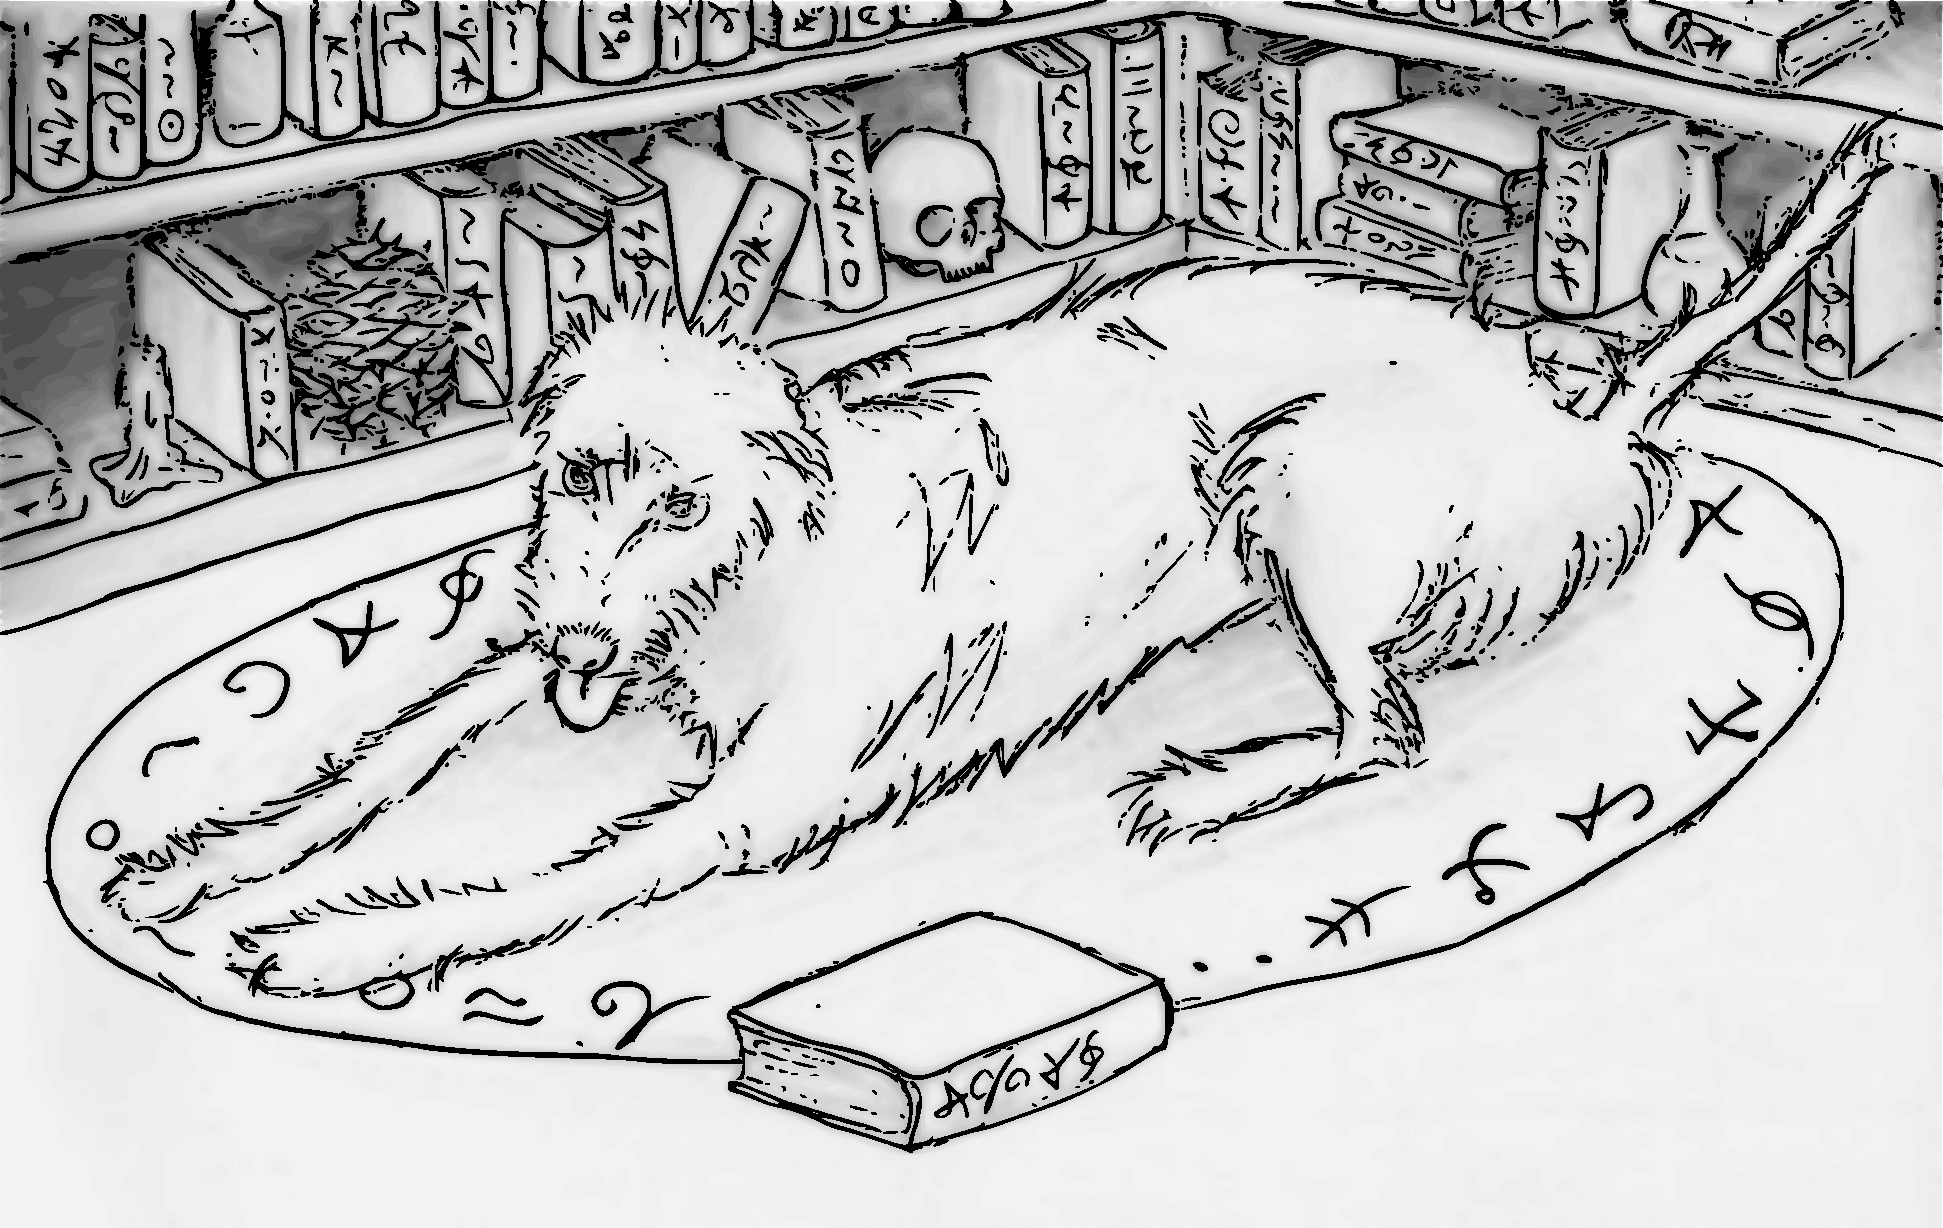
\includegraphics[width=\columnwidth]{fiona.pdf}\label{fiona}

\begin{multicols}{2}

The GM secretly rolls to determine the type of familiar, if any.  This spell does not function underwater unless cast by a naturally aquatic intelligent species, using different material components.  Other intelligent species may also have their own versions of the spell to summon a familiar specific to their environs and/or needs.  

The animals listed on the table should represent the most widespread and commonly desirable familiars among the PC races.  Some possible substitutions are listed on the table, but the GM is free to substitute any similar animals, no more than 18" in size, using the same or similar sensory powers.  Impossibly large insects have been listed on the table, and the GM may determine an animal on the table is not available in the area.  Any result can be ignored if the GM wishes by adding/subtracting 1 from the roll.  Due to extra-planar monitoring of this spell, the GM may determine that a caster will never summon an animal representing a diametrically opposed faith.  This becomes particularly important if the caster is multi-classed with priest.

If the master is 3\textsuperscript{rd} level or higher and the result of the d20 roll is between 16--20, subtract 1 from it per every 3 caster levels, and if that result is less than or equal to 15, roll again for the type of familiar using a d16 (1d8 with 1d6 high or low control die), and if a 16 (an 8 on 1d8 and a 4--6 on 1d6) is rolled, then no familiar is within spell range.

All familiars gain special abilities depending on its master's level.

\noindent
\begin{tabular}{|p{.18\columnwidth}|p{.07\columnwidth}|p{.07\columnwidth}|p{.07\columnwidth}|p{.36\columnwidth}|}
\hline
Master's Level	& AC Mod	& Int	& Size	& Powers \\
\hline\hline
\rowcolor[gray]{.9}1\textsuperscript{st}--2\textsuperscript{nd}	& $-1$	& 6		& 4"	& Shared Powers, Surprise Bonus, Telempathic Link \\
3\textsuperscript{rd}--4\textsuperscript{th} 	& $-2$	& 7		& 5"	& Deliver Touch Spells \\
\rowcolor[gray]{.9}5\textsuperscript{th}--6\textsuperscript{th}	& $-3$	& 8		& 7"	& Speak with Master \\
7\textsuperscript{th}--8\textsuperscript{th}	& $-4$	& 9		& 8"	& Speak with Animals of its Kind \\
\rowcolor[gray]{.9}9\textsuperscript{th}--10\textsuperscript{th}	& $-5$	& 10	& 10"	& -- \\
11\textsuperscript{th}--12\textsuperscript{th}	& $-6$	& 11	& 11"	& Magic Resistance \\
\rowcolor[gray]{.9}13\textsuperscript{th}--14\textsuperscript{th}	& $-7$	& 12	& 13"	& Scry on Familiar \\
15\textsuperscript{th}--16\textsuperscript{th}	& $-8$	& 13	& 14"	& -- \\
\rowcolor[gray]{.9}17\textsuperscript{th}--18\textsuperscript{th}	& $-9$	& 14	& 16"	& -- \\
19\textsuperscript{th}--20\textsuperscript{th}	& $-10$	& 15	& 18"	& -- \\
\hline
\end{tabular}

\textit{AC Modifier (Range---1 mile):} A familiar has a natural Armor Class of 7.  It gains a bonus to its armor class depending on the master's level. 

\textit{Intelligence (Range---Infinite):} This is the familiar's intelligence score, depending on the master's level. 

\textit{Size (Range---Infinite):} The familiar gets larger as the master increases in level, but will never exceed 18".

\noindent \underline{Powers}

\textit{Shared Hit Dice (Range---1 mile)}: For the purpose of effects related to number of Hit Dice, a familiar uses its master's character level.  Outside the range, a familiar has only $^1$/$_2$ HD.

\textit{Shared Hit Points (Range---1 mile)}: A familiar normally has only 2d2 hit points.  When in range, these hit points are added to the hit point total of its master, and the familiar adds $^1$/$_2$ the master's total hit points rounded down (and not including temporary or shared hit points) to its normal hit points. 

\textit{Shared Life Source (Range---Infinite)}: Beginning immediately after arriving, the familiar and its new master fuse their life sources.  The fate of one becomes inexorably linked to that of the other.  

This also means that the familiar gains either a soul or a spirit, depending upon its master, and a natural life span equal to its master's life span.  

If its master dies, the familiar permanently loses 1 hit point each day, and unless its master is brought back to life, dies when reaching 0 hit points.  If the master is restored to life, lost hit points return at the rate of 1 per day.

If the familiar dies before its master does, or is dismissed by its master for any reason, the master immediately loses 1 point of constitution and double the number (up to 8) of shared hit points.  The master may be killed if this sudden hit point loss reduces his current total below 0.  A slain familiar can be raised from the dead just as its master can, but it does not lose a point of constitution when raised.  If the familiar is successfully restored to life, the lost constitution is restored to its master instantly, and lost shared hit points are returned to the master at the rate of 1 per day.  A dismissed familiar reverts to its natural state and will never again respond to a call.    

A lost or dismissed familiar cannot be replaced for a year and day.  Due to the powerful magic involved, summoning a familiar can only be attempted once per year, and the use of this spell is monitored by certain, powerful extra-planar entities, such as the mysterious Animal Lords.  Abusing, neglecting or killing one's familiar will not go unnoticed or unpunished.  At the GM's discretion, special care and attention paid to a familiar may garner special favor from the extra-planar entities involved, usually when both master and familiar need help desperately.   

\textit{Shared Saving Throws (Range---5 feet)}: The familiar uses its master's saving throws, automatically succeeding if the master succeeds and failing if he fails.  The familiar takes no damage, if the save is successful, and only half the damage taken by its master, if the save fails.

\textit{Shared Spells (Range---5 feet)}: At the master's option, he may have any spell (but not innate abilities) he casts on himself also affect his familiar.  The spell stops affecting the familiar if it moves out of range and will not affect the familiar again even if it returns to the master before the duration expires.  Additionally, the master may cast a spell with an effective area of ``caster" on his familiar (as a touch spell) instead of on himself.  A master and his familiar can share spells even if the spells normally do not affect animals of the familiar's type. 
 
\textit{Shared THACO (Range---1 mile)}: A familiar uses its master's unmodified THACO.  Type of attack and damage is the same as that inflicted by a normal animal, usually 1d4 hit points if only one attack, or up to 3 attacks inflicting 1 and 1d2 hit points each, for example a claw/claw/bite attack that inflicts damage of 1/1/1d2.  Outside the range, THACO is calculated as a $^1$/$_2$ HD creature.

\textit{Surprise Bonus (Range---5 feet)}: The master gains +1 bonus to his surprise rolls.

\textit{Telepathic Link (Range---1 mile)}: The master and his familiar share a telempathic link that allows communication for up to 1 mile, but the master cannot see through the familiar's eyes.  The familiar communicates with basic, simple thoughts and emotions, limited by its intellect and natural instincts.

\textit{Deliver Touch Spells (Range---Touch)}: A familiar can deliver touch spells.  If the master and familiar are in contact at the time the master casts a touch spell, the familiar can then deliver the touch spell before the round ends just as the master could.  If the round ends before the touch is delivered, the spell fails. 
 
\textit{Speak with Master (Range---5 feet)}: A familiar and its master can communicate verbally, as if they were speaking a common language. Other creatures cannot understand the communication without magical assistance. 

\textit{Speak with Animals of its Kind (Range---Infinite)}: A familiar can communicate with animals of approximately the same kind as itself (including dire varieties): bats with bats, rats with rodents, cats with felines, hawks, owls and crows with birds, lizards and snakes with reptiles, toads with amphibians, weasels with similar animals (minks, polecats, ermines, skunks, wolverines, and badgers).  Such communication is limited by the intelligence of the conversing animals. 

\textit{Magic Resistance (Range---5 feet)}: A familiar gains magic resistance equal to the master's level~$\times$~5. 

\textit{Scry on Familiar (Range---1 mile/master's level)}: The master may scry on his familiar once per day.

\vspace{1em}

\noindent
\begin{minipage}{\columnwidth}

\noindent \textbf{\textit{Find the Path} (Greater Divination)}

\noindent \textbf{Caster/Level (Sphere):} Priest/6 (Divination)

\noindent \textbf{Range:} Touch

\noindent \textbf{Duration:} 1 turn/level

\noindent \textbf{Effective Area:} 1 creature

\noindent \textbf{Components:} V, S and M

\noindent \textbf{Casting Time:} 3 rounds

\noindent \textbf{Saving Throw:} None

\end{minipage}

This spell bestows upon the subject knowledge of the quickest, most direct route to and from any location, whether indoors, outdoors, in a town or underground, as long as it is on the same plane.  This knowledge comes slowly as needed by the subject, and not all at once.  The caster can be the subject of this spell.  The subject is shown, as he travels, the best route to reach his desired location, including which paths to follow and special actions required to avoid (but not disable) traps, such as when to step over a trip wire or what magic password is required to bypass a \textit{glyph of warding} or other magical trap.  The spell does not provide any knowledge to the subject's companions, and it cannot account for the presence of, nor predict the actions of, creatures that may be encountered along the route.  The spell ends when either the location is found or the duration expires.

The spell only works when a named or known location is referenced, and a character cannot find a location based solely on referencing a particular creatures or items.  ``Show me how to get to the white dragon's cave," will not work unless that is a name given by the subject to a location he has previously visited, or it is well known that there is a location called The White Dragon's Cave.  In the latter case, the subject will be pointed toward and slowly led to the nearest location with that name, though the dragon may have been slain or driven off years ago, or may never have even lived there at all.  It may not even be a real cave, but a tavern favored by local gangs of thieves and ruffians.

This spell is useful if trapped in a \textit{maze} spell.  The subject can escape and lead his companions out of the effective area of the \textit{maze} spell in 1 round.  This does not end the \textit{find the path} spell; so subsequent \textit{maze} effects will be similarly thwarted in 1 round until the \textit{find the path} spell ends normally.

The reverse, \textit{lose the path}, requires a successful touch attack.  It causes the subject to become lost, unable to find its way, for the duration of the spell, but the subject is able to follow someone else.

The material component is a set of divination tokens, such as bones, ivory counters, cards, sticks, carved runes, etc.  The reverse requires a marked or biased set of the same.

\vspace{1em}

\noindent
\begin{minipage}{\columnwidth}

\noindent \textbf{Find Traps (Lesser Divination)}

\noindent \textbf{Caster/Level (Sphere):} Priest/2 (Divination)

\noindent \textbf{Range:} 0

\noindent \textbf{Duration:} 3 turns

\noindent \textbf{Effective Area:} 10 feet~$\times$~30 yards

\noindent \textbf{Components:} V and S

\noindent \textbf{Casting Time:} 5

\noindent \textbf{Saving Throw:} None

\end{minipage}

This spell allows the caster to find any active trap, whether mundane or magical and regardless of the means used to conceal it, within the effective area directly in front of him.  For the purposes of this spell, a trap is any device or magical effect that was intentionally designed to inflict a sudden, unexpected and undesirable or harmful effect as a direct result of some action or inaction on the part of the intended victim.  Traps include \textit{alarm}, \textit{glyph of warding}, or similar combinations of spells and mechanisms.  The spell cannot predict ambushes or other actions that creatures may make, likewise, natural hazards or old, crumbly walls are not considered traps, as they were not originally designed to cause harm. 

The caster immediately learns whether a found trap is magical, mechanical, or both, but not its effect or how to disarm it.  Closer scrutiny, however, will reveal to the caster what actions or inactions may trigger it, and if the GM has determined that specific \textit{glyphs} or \textit{symbols} are associated with certain magical traps, closer scrutiny will also reveal the shape of the mark. 

\vspace{1em}

\noindent
\begin{minipage}{\columnwidth}

\noindent \textbf{Finger of Death (Necromancy)}

\noindent \textbf{Caster/Level:} Wizard/7

\noindent \textbf{Range:} 60 yards

\noindent \textbf{Duration:} Permanent

\noindent \textbf{Effective Area:} 1 creature pointed to

\noindent \textbf{Components:} V and S

\noindent \textbf{Casting Time:} 5

\noindent \textbf{Saving Throw:} Negate

\end{minipage}

This spell attempts to utterly destroy a chosen victim's life energy and body.  The victim must make a successful saving throw or die immediately, unable to be raised, resurrected, or reincarnated.  A \textit{wish} spell can restore most victims to life, if, however, the victims are human, profane magic instantly begins to transform the bodies, and after 3 days, the caster is able to perform a special ritual, requiring materials costing 1,000 gp~+~500 gp per body, to animate the dead humans as juju zombies under his control.  The profane magic must be reversed with a \textit{limited wish} spell before the juju animation ritual has begun, and then a \textit{wish} spell can be used to bring the human back to life.

Creatures who make a successful saving throw only suffer 2d8~+~1 points of damage.  If the victim dies due to this damage, they can be brought back to life normally.

\vspace{1em}

\noindent
\begin{minipage}{\columnwidth}

\noindent \textbf{Fire Charm (Enchantment)}

\noindent \textbf{Caster/Level:} Wizard/4

\noindent \textbf{Range:} 10 yards

\noindent \textbf{Duration:} 2 rounds/level

\noindent \textbf{Effective Area:} 15-foot radius

\noindent \textbf{Components:} V, S and M

\noindent \textbf{Casting Time:} 4

\noindent \textbf{Saving Throw:} Negate

\end{minipage}

This spell causes a veil of multicolored flame to surround a source of otherwise non-magical fire up to the size of the area of effect.  The veil is considered non-magical fire, so that those passing through it take the same amount of damage as if they had passed through the original fire source.  Creatures observing the dancing flames must make a successful saving throw, modified by wisdom-mental defense modifier or become charmed to stand motionless fixated on the flames.  Once charmed, each creature is subject to a single, individualized \textit{suggestion} of no more than 12 words each (as the spell, but with a maximum duration of 1 hour).  The charmed creatures are entitled to another saving throw, modified by wisdom-mental defense modifier and a $-3$ penalty, to resist the \textit{suggestion}.  The charm is broken if the creature is attacked, its view of the flames is blocked, or the duration expires.  If the GM allows, creatures that have broken the charm, but are re-exposed to the flames, can be subject to their effects again, but they will likely be entitled to bonuses on their saves of between +4 and +7 (to offset the $-3$ penalty).

The material component is a small, exceptionally thin piece of multicolored silk that the caster throws into the fire source.

\vspace{1em}

\noindent
\begin{minipage}{\columnwidth}

\noindent \textbf{Fire Seeds (Conjuration)}

\noindent \textbf{Caster/Level (Sphere):} Priest/6 (Elemental (Fire))

\noindent \textbf{Range:} Touch

\noindent \textbf{Duration:} 1 turn/level

\noindent \textbf{Effective Area:} Special

\noindent \textbf{Components:} V, S and M

\noindent \textbf{Casting Time:} 1 round/seed

\noindent \textbf{Saving Throw:} Half 

\end{minipage}

This spell has two effects.  The specific effect is chosen when the spell is cast.

\textbf{Acorn Grenades:} This effect transforms up to 4 acorns into indirect missiles that can be thrown up to a maximum of 40 yards.  Range modifiers are ignored, but an attack roll, modified by dexterity-missile attack modifier, is required to hit a specific target.  Roll on the indirect missile diagram to determine where a missed attack lands.  The acorns burst on impact; inflicting 2d8 hit points~+~1 per caster level of fire damage within a 10-foot radius, and igniting combustibles that fail a save vs. magical fire.  Creatures struck by a direct hit take full damage with no saving throw allowed.  Others within the burst area are allowed a saving throw, modified by dexterity-surprise modifier, to reduce the damage by half. 

\textbf{Holly Berry Bombs:} This effect transforms up to 8 holly berries into fiery bombs.  They work best when placed as remotely triggered bombs, exploding when the caster speaks the command word within 40 yards of where they are placed.  The berries are too light to be thrown effectively, exploding only 1d6 feet away.  They inflict 1d8 hit points~+~1 per caster level of fire damage within a 5-foot diameter burst, and igniting combustibles that fail a save vs. magical fire.  Those within the burst area are allowed a saving throw, modified by dexterity-surprise modifier, to reduce the damage by half. 
 
The material component is the appropriate seed (acorn or holly berry) for the specified effect.  Once enchanted, the seeds retain their effectiveness for the duration of the spell.

\vspace{1em}

\noindent
\begin{minipage}{\columnwidth}

\noindent \textbf{Fire Shield (Evocation, Transmutation)}

\noindent \textbf{Caster/Level:} Wizard/4

\noindent \textbf{Range:} 0

\noindent \textbf{Duration:} 2 rounds~+~1 round/level

\noindent \textbf{Effective Area:} The caster

\noindent \textbf{Components:} V, S and M

\noindent \textbf{Casting Time:} 4

\noindent \textbf{Saving Throw:} None

\end{minipage}

This spell allows the caster to create either a warm shield that protects against cold attacks or a chill shield that protects against fire attacks.  Both effects also cause damage to those attempting melee combat with the caster.  The specific effect is chosen when the spell is memorized.  When cast, the caster is engulfed completely by thin, wispy flames that emit no heat and shed half the light of a torch.

Melee attacks against the caster inflict normal damage, but the shield inflicts an equal amount of fire (warm shield) or cold (chill shield) damage to the attacker.  If the attacker has magic resistance, it's checked on the first successful hit, and the spell ends if the magic resistance check succeeds.  If the check fails, no further checks are made.

\textbf{Warm Shield:}  These flames are either blue or violet (random 50\% chance for either), and if touched, are warm.  The caster gains a +2 bonus to save against cold-based attacks and suffers only half damage (if save fails) or no damage (if save succeeds).  Fire-based attacks inflict double normal damage against the caster.  If no save is allowed or the save is failed, damage is doubled, and if the save is successful, the damage is full.

The material component for a warm shield is a bit of phosphorous.

\textbf{Chill Shield:}  These flames are either blue or green (random 50\% chance for either), and if touched, are cool.  The caster gains a +2 bonus to save against fire-based attacks and suffers only half damage (if save fails) or no damage (if save succeeds).  Cold-based attacks inflict double normal damage against the caster.  If no save is allowed or the save is failed, damage is doubled, and if the save is successful, the damage is full.

The material component for a chill shield is a live firefly or glowworm, or the tails of four dead ones.

\vspace{1em}

\noindent
\begin{minipage}{\columnwidth}

\noindent \textbf{\textit{Fire Storm} (Evocation)}

\noindent \textbf{Caster/Level (Sphere):} Priest/7 (Elemental (Fire))

\noindent \textbf{Range:} 160 yards

\noindent \textbf{Duration:} 1 round

\noindent \textbf{Effective Area:} two 10-foot cubes/level

\noindent \textbf{Components:} V and S

\noindent \textbf{Casting Time:} 1 round

\noindent \textbf{Saving Throw:} Half

\end{minipage}

With this spell, the caster engulfs the effective area with roaring flames equal in intensity to a \textit{wall of fire}, and igniting combustibles that fail their save vs. magical fire.  Creatures within the effective area, and up to 10 feet away from it, suffer 2d8 points of damage~+~1 per caster's level each round.  A successful saving throw, modified by dexterity---surprise modifier, reduces damage by half.  The height of the storm can be only 10 or 20 feet, and any remaining effective area can only make it longer or wider.  This spell cannot be cast underwater.

The reverse, \textit{fire quench}, smothers magical fires within the effective area, and normal fires within twice the effective area.  Extra-planar fire-based creatures of less than demigod status have a 5\% chance per caster level of being killed (if not on their home plane) when targeted by this spell.  If targeted against a \textit{flame tongue sword}, the wielder must save vs. spell, modified by dexterity---surprise modifier, and if this save fails, the sword must then save vs. crushing blow to avoid being rendered permanently mundane.

\vspace{1em}

\noindent
\begin{minipage}{\columnwidth}

\noindent \textbf{Fire Trap (Abjuration, Evocation)}

\noindent \textbf{Caster/Level (Sphere):} Priest/2 (Elemental (Fire)), Wizard/4

\noindent \textbf{Range:} Touch

\noindent \textbf{Duration:} Permanent until discharged

\noindent \textbf{Effective Area:} 1 object

\noindent \textbf{Components:} V, S and M

\noindent \textbf{Casting Time:} 1 turn

\noindent \textbf{Saving Throw:} Half

\end{minipage}

This spell is to be cast on a selected point on any object that can be closed, stoppered, latched and/or locked such as a book, box, bottle, chest, door, etc.  The fire trapped object cannot have a second magical trap, ward or lock a placed on it; attempting to do so negates the fire trap 25\% of the time, the secondary spell 25\% of the time, or both spells 50\% of the time.  If a creature other than the caster (and those designated when the spell is cast) intentionally opens the object, the trap explodes in a 5-foot radius inflicting 1d4 points of damage +1 per caster level.  A successful saving throw, modified by dexterity-surprise modifier, reduces damage by half.  The explosion does not harm the trapped item.  The explosion inflicts only half damage and creates a large steam cloud, if it occurs on an object submerged in water.

A knock spell does not trigger nor remove the trap.  The trap will still explode when the object is opened or entered by a non-designated creature.  Thieves and others skilled at find/remove traps treat this as a magical trap.  The trap explodes if an attempt to remove it fails.  The spell is permanent until the trap explodes or a successful dispel magic is cast.  An unsuccessful dispel magic does not cause the trap to explode. 

The priests' version of this spell functions the same as the wizards' version, only the material components are different.  

The material component for the wizards' version of this spell is either a bit of sulphur or saltpeter, which the caster must use to trace an outline around the closure and then touch to the selected point on the object.  The priests' version of this spell requires the caster to trace the outline of the closure with a stick of charcoal and touch the selected point with holly berries.  To designate a creature requires either caster to have a piece of hair, scale, claw, etc. from the creature.

\vspace{1em}

\noindent
\begin{minipage}{\columnwidth}

\noindent \textbf{Fireball (Evocation)}

\noindent \textbf{Caster/Level:} Wizard/3

\noindent \textbf{Range:} 10 yards~+~10 yards/level

\noindent \textbf{Duration:} Instantaneous

\noindent \textbf{Effective Area:} 20-foot radius sphere

\noindent \textbf{Components:} V, S and M

\noindent \textbf{Casting Time:} 3

\noindent \textbf{Saving Throw:} Half

\end{minipage}

With this spell, the caster launches a streak of fire from the his extended finger, which explodes into a roaring burst of flames upon reaching the distance and height selected by the caster (within the spell's range), inflicting 1d6 points of damage per caster level, up to a maximum of 10d6 to any creature in the effective area.  A successful saving throw, modified by dexterity---surprise modifier, reduces the damage by half.  If the initial trail of fire streaking from the caster's finger happens to strike a solid object before reaching it's intended detonation point, it immediately explodes.  A \textit{fireball} causes almost no structural damage, though it may be able to destroy weak wooden doors and windows (saving throw applicable) or blast open unlatched doors at the GM's discretion.  If a spherical burst is not possible, the effective area expands and spreads within its confinement up to the fullest extent of its effective volume (33,000 cubic feet) possible.  Unattended items in the effective area and items in the possession of those creatures failing their saving throw must also save vs. magical fire or be destroyed. 

The material components are a tiny ball of bat guano and sulphur.

\vspace{1em}

\noindent
\begin{minipage}{\columnwidth}

\noindent \textbf{Flame Arrow (Conjuration)}

\noindent \textbf{Caster/Level:} Wizard/3

\noindent \textbf{Range:} 30 yards~+~10 yards/level

\noindent \textbf{Duration:} 1 round

\noindent \textbf{Effective Area:} Special

\noindent \textbf{Components:} V, S and M

\noindent \textbf{Casting Time:} 3

\noindent \textbf{Saving Throw:} None or Half

\end{minipage}

This spell has two effects.  The specific effect is chosen when the spell is memorized.

\textbf{Magical Flaming Missiles:} The caster can use this spell for one round of personal missile combat.  This effect allows the caster to throw magical flaming bolts, 1 per 5 caster levels, at one or more opponents.  Multiple opponents must be within range, within 20 yards of each other, and the caster must be facing them.  Each missile inflicts 1d6 points of damage plus 4d6 points of fire damage on a successful hit.  A successful saving throw, modified by dexterity-surprise modifier, by the opponent(s) against each successful hit reduces the fire damage by half.  The effect is not considered a magical weapon and cannot overcome weapon immunities, nor will it function underwater.

\textbf{Mundane Flaming Missiles:} Used mostly during large-scale battles, this effect allows the caster to ignite up to 10 mundane arrows or crossbow bolts per 5 caster levels with magical flames.  The bowmen must be within the spell's range and arranged in a tight formation within 5 feet of each other.  The missiles must be drawn or cocked by the end of the casting time.  Each missile then inflicts 1 point of fire damage in addition to their normal damage.  The arrows or bolts must be fired within the spell's duration, or the magical flames consume them.

The material components for either effect are a small piece of flint and a drop of oil.

\vspace{1em}

\noindent
\begin{minipage}{\columnwidth}

\noindent \textbf{Flame Blade (Evocation)}

\noindent \textbf{Caster/Level (Sphere):} Priest/2 (Elemental (Fire))

\noindent \textbf{Range:} 0

\noindent \textbf{Duration:} 4 rounds~+~1 round/2 levels

\noindent \textbf{Effective Area:} 3-foot long blade

\noindent \textbf{Components:} V, S and M

\noindent \textbf{Casting Time:} 4

\noindent \textbf{Saving Throw:} None

\end{minipage}

By the use of this spell, the caster creates a fiery, magical blade.  The ``blade" springs from the caster's hand and can be wielded as if it were a weapon the caster is able to use.  A successful hit inflicts 1d4~+~4 points of fire damage, however, an additional 2 points of fire damage is inflicted against the undead or those particularly vulnerable to fire, while creatures magically protected or resistant to fire subtract 2 points of damage.  The blade causes combustible materials such as parchment, straw, dry sticks, cloth, etc. to make a successful saving throw against magical fire or ignite on contact.  Extra-planar fire creatures, those immune to fire or who have natural fire-based attacks are immune to the damage.  The effect is not considered a magical weapon and cannot overcome weapon immunities (except when used against the undead), nor does it function underwater.

The material components are the caster's holy or unholy symbol and a leaf of sumac.

\vspace{1em}

\noindent
\begin{minipage}{\columnwidth}

\noindent \textbf{Flame Strike (Evocation)}

\noindent \textbf{Caster/Level (Sphere):} Priest/5 (Combat)

\noindent \textbf{Range:} 60 yards

\noindent \textbf{Duration:} Instantaneous

\noindent \textbf{Effective Area:} 5-foot radius~$\times$~30-foot column

\noindent \textbf{Components:} V, S and M

\noindent \textbf{Casting Time:} 8

\noindent \textbf{Saving Throw:} Half

\end{minipage}

This spell creates a vertical column of roaring fire, inflicting 6d8 points of damage and igniting combustibles within the effective area that fail their save vs. magical fire.  A successful save, modified by dexterity---surprise modifier, reduces damage by half.

The material component is a pinch of sulphur.

\vspace{1em}

\noindent
\begin{minipage}{\columnwidth}

\noindent \textbf{Flame Walk (Transmutation)}

\noindent \textbf{Caster/Level (Sphere):} Priest/3 (Elemental (Fire))

\noindent \textbf{Range:} Touch

\noindent \textbf{Duration:} 1 round~+~1/level

\noindent \textbf{Effective Area:} 1 or more creatures

\noindent \textbf{Components:} V, S and M

\noindent \textbf{Casting Time:} 5

\noindent \textbf{Saving Throw:} None

\end{minipage}

When casting this spell, the caster touches 1 creature (or themselves) plus up to one additional creature per caster level above 5.  The selected subjects are able to endure non-magical fires with temperatures ranging up to 2,000$^\circ$F (molten lava would not harm the subject).  Saving throws vs. magical fires are made with a +2 bonus, and any damage is reduced to half or one-quarter.  \textit{Flame walk} is not cumulative with \textit{resist fire} or similar fire protection spells.

The material components of the spell are the caster's holy or unholy symbol and powdered ruby worth at least 500 gp per selected creature.

\vspace{1em}

\noindent
\begin{minipage}{\columnwidth}

\noindent \textbf{Flaming Sphere (Evocation)}

\noindent \textbf{Caster/Level:} Wizard/2

\noindent \textbf{Range:} 10 yards

\noindent \textbf{Duration:} 1 round/level

\noindent \textbf{Effective Area:} 3-foot radius

\noindent \textbf{Components:} V, S and M

\noindent \textbf{Casting Time:} 2

\noindent \textbf{Saving Throw:} Negate

\end{minipage}

This spell creates a burning globe of fire anywhere within the spell's range.  The sphere remains at rest unless the caster actively directs it.  The sphere rolls, at a rate of 30 feet per round, in any direction the caster points, but the mage must be able to see the sphere at all times.  It rolls over solid barricades of less than 4-feet tall, and combustible materials touched by the sphere must make a successful saving throw vs. magical fire or catch fire.  A creature struck by the sphere must save vs. spell, modified by dexterity---surprise modifier, or suffer 2d4 points of fire damage, and those within 5 feet of the sphere must save vs. spell, modified by dexterity---surprise modifier, or suffer 1d4 points of heat damage.  In any case, a successful saving throw means the creature takes no damage from the effect.  The sphere is a sponge like mass, inflicting damage only via its heat, and cannot batter or push aside creatures or objects. The sphere can be extinguished as if it were a normal fire filling the effective area. 

The material component requirements to cast this spell are a small amount of tallow, and a dash each of sulphur and powdered iron dust.

\noindent
\includegraphics[width=3.6in, height=1.75in]{testblock.pdf}

\vspace{1em}

\noindent
\begin{minipage}{\columnwidth}

\noindent \textbf{Floating Disc (Evocation)}

\noindent \textbf{Caster/Level:} Wizard/1

\noindent \textbf{Range:} 20 yards

\noindent \textbf{Duration:} 3 turns~+~1 turn/level

\noindent \textbf{Effective Area:} Special

\noindent \textbf{Components:} V, S and M

\noindent \textbf{Casting Time:} 1

\noindent \textbf{Saving Throw:} None

\end{minipage}

This spell creates a slightly concave, circular disc of force.  The disc is 3 feet in diameter, always floats at a level 3 feet above the ground, and can hold up to 100 pounds of weight per caster level or up to 2 gallons of liquid.  It moves as directed by the caster with a movement value of 6, or if left unguided, it attempts to maintain a constant distance of 6 feet away from the caster.  If the disc moves outside its range, gets lifted more than 3 feet above the ground, or the duration expires, it vanishes and drops anything it was carrying.  The caster cannot ride the disc.

The material component is a drop of quicksilver (mercury).

\vspace{1em}

\noindent
\begin{minipage}{\columnwidth}

\noindent \textbf{Fly (Transmutation)}

\noindent \textbf{Caster/Level:} Wizard/3

\noindent \textbf{Range:} Touch

\noindent \textbf{Duration:} 1 turn/level~+~1d6 turns

\noindent \textbf{Effective Area:} 1 creature

\noindent \textbf{Components:} V, S and M

\noindent \textbf{Casting Time:} 3

\noindent \textbf{Saving Throw:} None

\end{minipage}

This spell allows the caster, or a subject touched by the caster, to magically fly, able to move vertically or horizontally at a movement value of 18 (MC2 and SC2---good and average).  Flying requires little concentration, so that spells can be cast if the flyer hovers or reduces its movement value to 3 (SC1) for that round.  The GM rolls the variable duration of the spell secretly.  (Refer to Aerial Combat for further details regarding flight).  This spell also allows its recipient to swim at any depth desired with little effort, even if too heavy or encumbered to swim normally.  The recipient's maximum swim speed is 9.

The material component is a wing feather of any bird.

\vspace{1em}

\noindent
\begin{minipage}{\columnwidth}

\noindent \textbf{Fog Cloud (Transmutation)}

\noindent \textbf{Caster/Level:} Wizard/2

\noindent \textbf{Range:} 10 yards

\noindent \textbf{Duration:} 4 rounds~+~1 round/level

\noindent \textbf{Effective Area:} Special

\noindent \textbf{Components:} V and S

\noindent \textbf{Casting Time:} 2

\noindent \textbf{Saving Throw:} None

\end{minipage}

This spell has two effects.  The specific effect is chosen when the spell is cast. 

Both effects obscure all sight, including infravision, beyond 2 feet within the effective area, but are otherwise harmless.  A strong breeze will disperse either effect in one round, and a moderate breeze will reduce the duration by 50\%.  The spell cannot be cast underwater.

\textbf{Fog Bank:} This effect creates a stationary bank of greenish-grey fog, of any shape and anywhere within range, up to a 20-foot cube per caster level in size. 

\textbf{Billowy Vapors:} This effect creates billowing vapors that look and move exactly like a cloud kill spell.  

\vspace{1em}

\noindent
\begin{minipage}{\columnwidth}

\noindent \textbf{Fool's Gold (Transmutation, Illusion)}

\noindent \textbf{Caster/Level:} Wizard/2

\noindent \textbf{Range:} 10 yards

\noindent \textbf{Duration:} 1 hour/level

\noindent \textbf{Effective Area:} 10 cubic inches/level

\noindent \textbf{Components:} V, S and M

\noindent \textbf{Casting Time:} 1 round

\noindent \textbf{Saving Throw:} Special

\end{minipage}

This spell transforms copper, bronze or brass items into gold for the spell's duration. The effective area is the equivalent of 150 coins per caster level.  Creatures viewing the gold can discern its original nature by saving vs. spell, modified by wisdom-mental defense modifier and a $-1$ penalty per caster level.  If roughly struck with cold wrought iron, there's a chance the gold will revert to its original form.  Rare and expensive material components reduce this chance.

The caster selects which material component to sprinkle on the object when casting this spell.  If powdered citrine worth at least 25 gp is used, the chance of being detected by cold iron is 30\%, if at least 50 gp worth of powdered amber is used, the chance of being detected is 25\%, if at least 250 gp worth of powdered topaz is used, the chance of being detected is 10\%, and if at least 500 gp worth of powdered corundum (oriental topaz) is used, the chance of being detected by cold iron drops to only 1\%.

\vspace{1em}

\noindent
\begin{minipage}{\columnwidth}

\noindent \textbf{Forbiddance (Abjuration)}

\noindent \textbf{Caster/Level (Sphere):} Priest/6 (Protection)

\noindent \textbf{Range:} 30 yards

\noindent \textbf{Duration:} Permanent

\noindent \textbf{Effective Area:} 60-foot cube/level

\noindent \textbf{Components:} V, S and M

\noindent \textbf{Casting Time:} 6 rounds

\noindent \textbf{Saving Throw:} Special

\end{minipage}

This spell attempts to prevent any unwanted or unauthorized entry into a consecrated area (Refer to Crafting Magical Items), including entry by magical means such as \textit{teleport}, \textit{plane shifting}, and \textit{ethereal travel}.  

The caster can either leave the area unlocked or lock the area with a password to allow creatures speaking it to enter.  Only a caster of equal or higher level than the original caster has a chance to end the ward with a \textit{dispel magic}.  Creatures violating the ward suffer effects based on their alignment with respect to the caster's alignment, and the most severe effect is used.

\textbf{Identical Alignment:} If password locked, a creature simply speaks the password to enter the consecrated area.  If unlocked, a creature can enter the area at will.

\textbf{Alignment different on the law vs. chaos scale:} If a creature speaks the password, he can enter the consecrated area at will.  If the area is not locked, a creature makes a saving throw vs. spell to attempt to enter the consecrated area.  If a creature fails this save, it suffers 2d6 points of damage and is blocked out of the consecrated area for the duration of the spell.  

\textbf{Alignment different on the good vs. evil scale:} The creature makes a saving throw vs. spell to attempt to enter the consecrated area whether the area is unlocked or the password is known.  If the creature fails this save, it suffers 4d6 points of damage and is blocked out of the consecrated area for the duration of the spell. 

Those unauthorized intruders who enter by rolling a successful save feel nervous and on edge while in the effective area, despite their success.

The material components are the caster's holy or unholy symbol, holy or unholy water, and rare incenses worth 1,000 gp per each 60-foot cube of effective area.  If the area is to be password locked, an additional 5,000 gp worth of incense per 60-foot cube is needed.

\vspace{1em}

\noindent
\begin{minipage}{\columnwidth}

\noindent \textbf{Force Cage (Evocation)}

\noindent \textbf{Caster/Level:} Wizard/7

\noindent \textbf{Range:} 10 yards/2 levels

\noindent \textbf{Duration:} 6 turns~+~1/level

\noindent \textbf{Effective Area:} 20-foot cube

\noindent \textbf{Components:} V, S and M

\noindent \textbf{Casting Time:} 3 (4 force cube effect)

\noindent \textbf{Saving Throw:} None

\end{minipage}

This spell has two effects.  The specific effect is chosen when the spell is memorized.

\textbf{Force Cage:} This effect allows the caster to create a cage made of force, anywhere within range and filling the effective area.  The walls of the cage are not solid but are made of alternating bands with $^1$/$_2$-inch gaps between them, like a prison cell.  Creatures within the effective area when the spell is cast are trapped, unless they can slip between the bars, but most effects from spells or special abilities can pass through the gaps in the bars of force easily.  If a trapped creature has magic resistance, it is checked only once to attempt to pass through the force bars.  A successful magic resistance check does not destroy the cage or allow other creatures (except a personal familiar) to escape.  The cage stays in effect until the duration expires or until a successful dispel magic is cast.

\textbf{Force Cube:} With this effect, the effective area is halved and the walls are made solid.  This effect then functions as the magical item, cube of force, except for the intrinsic differences between using a magic item and casting a spell.  

The material component for either spell effect is diamond dust worth at least 1,000 gp.  During memorization of the preferred spell effect, the caster uses the diamond dust to trace an outline of the desired type of cage.  Once the effect is memorized, the diamond dust is scattered to the wind, and is no longer needed to cast the spell.

\vspace{1em}

\noindent
\begin{minipage}{\columnwidth}

\noindent \textbf{Foresight (Greater Divination)}

\noindent \textbf{Caster/Level:} Wizard/9

\noindent \textbf{Range:} 0

\noindent \textbf{Duration:} 2d4 rounds~+~1 round/level

\noindent \textbf{Effective Area:} Special

\noindent \textbf{Components:} V, S and M

\noindent \textbf{Casting Time:} 1 round

\noindent \textbf{Saving Throw:} None

\end{minipage}

This spell grants the caster extraordinary danger sense with respect to himself or any other designated creature.  While the duration is in effect, the caster receives advanced warnings to impending harm or danger to the subject.  This includes ambushes, other unseen attackers (melee or missile), dangerous natural settings, and all kinds of traps.  If the caster is the subject of the spell, he cannot be surprised.  He also gains a $-2$ bonus to his armor class and a +2 bonus to any necessary saving throws.  

If another creature is the subject of the spell, it cannot be surprised so long as the caster concentrates on it and communicates the warnings to it without hesitation, but the subject does not gain a bonus to his armor class or saving throws.

The material component is a feather from a hummingbird.

\noindent
\includegraphics[width=3.6in, height=2.25in]{testblock.pdf}


\vspace{1em}

\noindent
\begin{minipage}{\columnwidth}

\noindent \textbf{Forget (Enchantment)}

\noindent \textbf{Caster/Level:} Wizard/2

\noindent \textbf{Range:} 30 yards

\noindent \textbf{Duration:} Permanent

\noindent \textbf{Effective Area:} 20-foot cube

\noindent \textbf{Components:} V and S

\noindent \textbf{Casting Time:} 2

\noindent \textbf{Saving Throw:} Negate

\end{minipage}

This spell attempts to cause creatures to forget the events of the previous round (or the previous minute of non-combat game time), plus an additional round (or minute) per three caster levels.  The spell does not negate \textit{charm}, \textit{suggestion}, \textit{geas}, \textit{quest}, or similar spells, but it's possible to forget who cast the spell.  

The caster can choose to affect between 1--4 creatures within the effective area.  The creatures are granted saving throws, modified by wisdom---mental defense modifier, to avoid the effect completely.  If only one creature is targeted, it saves with an additional $-2$ penalty, if two creatures are affected, they each suffer an additional $-1$ penalty, and if three or four are affected, a normal save is rolled.  It requires a specially worded \textit{heal}, \textit{restoration}, \textit{limited wish}, or \textit{wish} spell to restore memories lost to this spell.

\vspace{1em}

\noindent
\begin{minipage}{\columnwidth}

\noindent \textbf{Free Action (Abjuration, Enchantment)}

\noindent \textbf{Caster/Level (Sphere):} Priest/4 (Charm)

\noindent \textbf{Range:} Touch

\noindent \textbf{Duration:} 1 turn/level

\noindent \textbf{Effective Area:} 1 creature

\noindent \textbf{Components:} V, S and M

\noindent \textbf{Casting Time:} 7

\noindent \textbf{Saving Throw:} None

\end{minipage}

This spell allows the caster to touch a creature and enable it to move and act normally, even under the influence of magic that restricts or impedes movement, such as hold, paralysis, \textit{slow}, and even \textit{web} or \textit{entangle} spells.  The caster may choose to be the recipient. The creature can also slip out of the tightest of mundane bonds or snares.  Underwater, the creature can move at his normal swimming speed and inflict normal damage with any melee weapon, but it cannot breathe underwater without other appropriate enchantments.

The material component is a leather thong, bound around the arm (or its equivalent), which \textit{disintegrates} when the spell expires.

\vspace{1em}

\noindent
\begin{minipage}{\columnwidth}

\noindent \textbf{Freezing Sphere (Transmutation, Evocation)}

\noindent \textbf{Caster/Level:} Wizard/6

\noindent \textbf{Range:} Special

\noindent \textbf{Duration:} Special

\noindent \textbf{Effective Area:} Special

\noindent \textbf{Components:} V, S and M

\noindent \textbf{Casting Time:} 6

\noindent \textbf{Saving Throw:} Special

\end{minipage}

This powerful spell allows the caster to create one of the following effects, chosen at the time of casting.

\textbf{Frigid Globe:} This effect creates a globe of absolute zero degrees that freezes up to 100 square feet of water per caster level, creating a solid sheet of ice 6 inches deep.  The ice lasts for one round per caster level. 

The material component for this effect is a thin, 1 square inch sheet of crystal.

\textbf{Cold Ray:} This effect creates a narrow ray of cold, extending 10 yards per caster level, from the caster's hand.  It inflicts 1d4~+~2 points of damage per caster level to the first creature it successfully hits.  If a targeted creature makes a successful save, modified by dexterity-surprise modifier, it indicates that it avoided the ray completely, but the ray continues in a straight line for its full distance until a creature behind the original creature fails its save (also modified by dexterity-surprise modifier), or until the ray finally strikes an inanimate object (doing full cold damage to the object, as applicable).  

The material component for this effect is a white sapphire worth at least 1,000 gp.  

\textbf{Globe of cold:}  This effect creates a slightly chilled globe the size of a sling stone that can be hurled by hand out to 40 yards (ignoring any range penalties) or used as a sling bullet.  The globe explodes on impact, inflicting 6d6 points of cold damage to all creatures within a 10-foot radius.  A successful saving throw, modified by dexterity-surprise modifier, reduces damage by half.  The globe is treated as an indirect missile, if an attack misses.  If the globe isn't hurled at an opponent within one round per caster level, it automatically explodes and inflicts damage as per normal.  The globe can be used in this manner to slow or incapacitate a pursuing creature, but it can also be quite dangerous for the caster and his allies.

The material component is a 1,000 gp diamond.

\vspace{1em}

\noindent
\begin{minipage}{\columnwidth}

\noindent \textbf{Friends (Enchantment)}

\noindent \textbf{Caster/Level:} Wizard/1

\noindent \textbf{Range:} 0

\noindent \textbf{Duration:} 1d4 rounds~+~1 round/level

\noindent \textbf{Effective Area:} 60-foot radius

\noindent \textbf{Components:} V, S and M

\noindent \textbf{Casting Time:} 1

\noindent \textbf{Saving Throw:} Special

\end{minipage}

This spell temporarily adds 2d4 points to the caster's charisma.  Intelligent creatures within the effective area when the spell is cast must immediately make a reaction check using the caster's new charisma.  Those who roll a favorable reaction result suddenly take a liking to the caster and want to be his friend.  For the spell's duration, they will make reasonable efforts to be as helpful as they can be, given the current situation and their nature.  When the spell ends, the affected creatures realize they've been influenced and may react badly, at the GM's discretion.

The material components are chalk or white flour, lampblack or soot, and vermilion applied to the caster's face before casting the spell.

\vspace{1em}

\noindent
\begin{minipage}{\columnwidth}

\noindent \textbf{Fumble (Enchantment)}

\noindent \textbf{Caster/Level:} Wizard/4

\noindent \textbf{Range:} 10 yards/level

\noindent \textbf{Duration:} 1 round/level

\noindent \textbf{Effective Area:} 30-foot cube

\noindent \textbf{Components:} V, S and M

\noindent \textbf{Casting Time:} 4

\noindent \textbf{Saving Throw:} Special

\end{minipage}

This spell has two effects.  The specific effect is chosen when the spell is cast.

\textbf{Area of Disorientation:} This effect allows the caster to create disorientation within the effective area, where each round, all creatures must make a successful saving throw, modified by wisdom---mental defense modifier, or become awkward and clumsy for that round.  Those that make their save can act normally that round, while those that fail the save will trip and fall, drop everything they are holding (weapons, magic items, material components, etc.), and fail at any actions that require manual dexterity.  The GM may decide that dropped items must make a saving throw to avoid being damaged or ruined.  Getting back on their feet and picking up their dropped items consumes a full round, as long as the new saving throw is successful or the spell has ended.

\textbf{One Clumsy Creature:} This effect is cast on a single creature.  The creature must make one successful saving throw, modified by wisdom-mental defense modifier, or suffer the effects of disorientation for the spell's entire duration.  Even with a successful saving throw, the creature is affected by the equivalent of a slow spell for the duration.

The material component for either effect is a dab of solidified milk fat.

\vspace{1em}

\noindent \textbf{\subsection{G}}

\noindent
\begin{minipage}{\columnwidth}

\noindent \textbf{Gate (Conjuration)}

\noindent \textbf{Caster/Level (Sphere):} Priest/7 (All), Wizard/9

\noindent \textbf{Range:} 30 yards

\noindent \textbf{Duration:} Special

\noindent \textbf{Effective Area:} Special

\noindent \textbf{Components:} V and S

\noindent \textbf{Casting Time:} Priest- 5, Wizard- 9

\noindent \textbf{Saving Throw:} None

\end{minipage}

Casting this spell produces two simultaneous effects.  The first effect notifies a powerful extra-planar creature that the caster wishes their assistance.  The second effect causes an extra-dimensional rift to open between the caster's current plane of existence and the desired creature's plane, which can simply be stepped through.  The caster must speak the name and type of creature he wishes to step through the \textit{gate} and assist him, giving their true name and title, if they have such.  

Either the named creature or one of his associates or minions will step through with 100\% certainty.  The exact creature is up to the GM.  What the creature does when it arrives depends on many factors, including the alignments of the caster and the creature, the nature of those accompanying the caster, and who or what opposes or threatens the caster.  The GM must determine the results, based on the creature called, the desires of the caster and the needs of the moment.  If the caster's problem is minor or insignificant to the creature, it may leave immediately, or inflict a punishment against the caster and then leave, or even attack the caster (though they are smart enough to avoid combat they cannot win).  If the caster has an urgent problem or one that interests the creature, it will usually agree to stay and help the caster in exchange for suitable repayment (Also Refer to the \textit{Exaction} spell).  

Casting this spell ages a caster five years if his venerable age is 150 years or less, ten years if his venerable age is between 151 and 250 years, 15 years if his venerable age is between 251 and 350 years, etc.

\vspace{1em}

\noindent
\begin{minipage}{\columnwidth}

\noindent \textbf{Gaze Reflection (Transmutation)}

\noindent \textbf{Caster/Level:} Wizard/1

\noindent \textbf{Range:} 0

\noindent \textbf{Duration:} 2 rounds~+~1 round/level

\noindent \textbf{Effective Area:} Special

\noindent \textbf{Components:} V and S

\noindent \textbf{Casting Time:} 1

\noindent \textbf{Saving Throw:} None

\end{minipage}

With this spell, the caster is fully protected from gaze attacks.  The caster causes the very air in front of him to become a gleaming, reflective surface that moves with him.  Though the caster can see through the effect normally, any active gaze attack, spell, or special ability that relies on eye contact is reflected, forcing the attacker to make a save vs. its own attack.  The spell has no affect on the ambient light or either party's vision, nor is it effective against creatures whose attack comes when simply being looked at.  

\vspace{1em}

\noindent
\begin{minipage}{\columnwidth}

\noindent \textbf{Geas (Enchantment)}

\noindent \textbf{Caster/Level:} Wizard/6

\noindent \textbf{Range:} 10 yards

\noindent \textbf{Duration:} Special

\noindent \textbf{Effective Area:} 1 creature

\noindent \textbf{Components:} V

\noindent \textbf{Casting Time:} 4

\noindent \textbf{Saving Throw:} None

\end{minipage}

This spell allows the caster to set a magical directive upon a creature either to perform a specific task, or to prohibit it from performing a certain activity.  The full and exact nature of the \textit{geas} must be specified while casting.  A \textit{geas} that is vaguely worded fails during casting.  The subject must be intelligent, awake, and able to understand the caster's language.  While it does not necessarily have to be willing, the subject cannot be under the effect of a charm or other enchantment magic.  

A \textit{geas} requiring a task is permanent until the task is finished successfully, or it is removed by a wish spell.  A \textit{geas} that forbids a certain activity is only removed by a \textit{wish} spell.

A \textit{geas} cannot force the subject to be suicidal (``Stop eating") or do foolish things likely to get it killed (``Throw down your sword and taunt that ancient red dragon"), but the subject will perform nearly any other task.  Usually, the tasks required or activities prohibited will be of much more monumental importance (``Fetch me the eye of the roc that has been terrorizing Sodville" or ``You may never enter Red Forest").

While there is no time limit to accomplish a required task, the subject must actively seek to accomplish his directive at all times, whether the directive is to do something or not do something.  Looking for an easy way out of performing the required task, deviating from the directive or performing the prohibited action, results in the subject losing one point of strength per day until the intentional deviation ceases, gradually becoming sick and dying when strength reaches 0.  Each point of strength lost requires one full day to recover.  The GM may assign harsher penalties for repeat, multiple and willful deviations and can decide upon an appropriate penalty to fit the situation.

\vspace{1em}

\noindent
\begin{minipage}{\columnwidth}

\noindent \textbf{\textit{Giant Insect} (Transmutation)}

\noindent \textbf{Caster/Level (Sphere):} Priest/4 (Animal)

\noindent \textbf{Range:} 20 yards

\noindent \textbf{Duration:} Permanent

\noindent \textbf{Effective Area:} 1 or more insects

\noindent \textbf{Components:} V, S and M

\noindent \textbf{Casting Time:} 7

\noindent \textbf{Saving Throw:} None

\end{minipage}

This spell causes a number of normal, non-magical insects, anywhere within range, to grow to giant size.  Only one type of insect can be affected per casting, and the insects are all grown to equal HD and size.  The maximum number of HD each insect can attain individually, and the maximum total HD the caster can bestow is determined by the caster's level.  Theoretically, a 10th level caster can grow 3 of the same type of insects to 4 HD each (3~$\times$~4 = 12), 4 insects to 3 HD each, 6 insects to 2 HD each, or 12 insects to 1 HD each, however, the real limiting factors are how many and what kinds of insects are within range.  The GM must determine this when the spell is being cast. 

\noindent
\begin{tabular}{|p{.25\columnwidth}|p{.3\columnwidth}|p{.3\columnwidth}|}
\hline
Caster Level	& Insect Max HD	& Maximum Total HD \\
\hline\hline
\rowcolor[gray]{.9}7--9	& 3	& 9 \\
10--12	& 4	& 12 \\
\rowcolor[gray]{.9}13+	& 6	& 15 \\
\hline
\end{tabular}

The GM may then use any pre-prepared combat and movement values as desired for the giant insects or consult the following table, which provides some basic guidelines.  Size is either length or height.  Carry refers to the weight it can carry on its back, while moving, or in its front claws (i.e. mantis).  If the insect has mandibles, lift refers to the weight the insect is able to lift and carry in its mandibles.  The item or creature being carried in the insect's mandibles takes normal damage on the ``first hit" or lift round and $^1$/$_2$ normal damage each round thereafter, until released.  An unwilling subject is granted a saving throw, modified by dexterity---surprise modifier, to avoid being lifted.

The giant insects won't harm the caster unless influenced by another magical effect after the insect is enlarged, but if left on their own, the giant insects will attack whoever or whatever else is nearby.  They can follow only simple, one word commands and hand gestures from the caster (stay, go, stop, run, fly, land, attack, guard, etc.).  If the caster is present, this is usually enough to protect his allies from attack.

If anything interrupts the casting or the insects were previously under the influence of any magical effect (including this spell, but not its reverse), the casting fails, and the insects die.  This spell has no effect on arachnids, crustaceans, other non-insect vermin, or intelligent insect-like creatures.

The reverse, \textit{shrink insect}, attempts to reduce one or more giant insects to their normal size.  The caster's maximum total HD (from the table above) is subtracted from the targeted giant insects' HD.  If a giant insect reaches 0HD, it becomes a normal-sized insect; otherwise, the spell has no effect.  If the effect would only partially shrink an insect, the spell fails.  For example, a 10\textsuperscript{th} level caster has a maximum total HD of 12, therefore, giant insects with 13 HD or more cannot be shrunk, but 1 giant insect with 12 HD or less, 2 giant insects with 6 HD or less each, 3 giant insects with 4 HD or less each, etc. are reduced to normal size.  As with the standard spell, the reverse has no effect on arachnids, crustaceans, other non-insect vermin, or intelligent insect-like creatures.

The material component for the spell and its reverse is the caster's holy or unholy symbol.

\end{multicols}

\noindent
\begin{tabular}{|p{.05\textwidth}|p{.05\textwidth}|p{.1\textwidth}|p{.1\textwidth}|p{.1\textwidth}|p{.2\textwidth}|p{.1\textwidth}|p{.1\textwidth}|}
\multicolumn{8}{c}{Giant Insect} \\
\hline
HD	& AC	& Dmg	& Size	& Weight	& Carry/Lift	& MC	& SC*** \\
\hline\hline
\rowcolor[gray]{.9}1	& 8	& 1d4	& 3'	& 50 lbs.	& 80 lbs./80 lbs.	& 3	& 3 \\
2	& 7	& 2d4	& 5'	& 230 lbs.	& 160 lbs./350 lbs.	& 3	& 3 \\
\rowcolor[gray]{.9}3*	& 6	& 3d4	& 7'	& 630 lbs.	& 240 lbs./1000 lbs.	& 4	& 2 \\
4	& 5	& 4d4	& 9'	& 1850 lbs.	& 320 lbs./2150 lbs.	& 4	& 2 \\
\rowcolor[gray]{.9}5	& 4	& 5d4	& 11'	& 2450 lbs.	& 400 lbs./3900 lbs.	& 5	& 1 \\
6**	& 3	& 6d4	& 13'	& 4060 lbs.	& 480 lbs./6500 lbs.	& 5	& 1 \\
\hline
\end{tabular}

\noindent\begin{tabular}{p{.98\textwidth}}
*Insects, including flying insects, grown to at least 3HD are usually large enough to carry a man-sized rider. \\
**Insects, including flying insects, grown to at least 6HD are usually large enough to carry 2 man-sized riders. \\
***Speed class can be roughly converted to movement value (See Aerial Combat). \\
\end{tabular}\vspace{.5em}

\begin{multicols}{2}

\vspace{1em}

\noindent
\begin{minipage}{\columnwidth}

\noindent \textbf{Glass See (Transmutation)}

\noindent \textbf{Caster/Level:} Wizard/6

\noindent \textbf{Range:} Touch

\noindent \textbf{Duration:} 1 round/level

\noindent \textbf{Effective Area:} 3-feet wide ~$\times$~2-feet high

\noindent \textbf{Components:} V, S and M

\noindent \textbf{Casting Time:} 1 round

\noindent \textbf{Saving Throw:} None

\end{minipage}

This spell causes a section of a piece of metal, stone, or wood, up to the size of the effective area, to become transparent.  Metal up to 4 inches thick, stone up to 6 inch thick, or wood up to 20 inches thick can be affected, however lead, gold, and platinum are immune. The caster can make the material transparent to only his vision or make the material a one-way window, allowing everyone on the caster's side to see through.  The affected area is still as strong as the original material.

The material component is a small piece of crystal or glass.
 
\vspace{1em}

\noindent
\begin{minipage}{\columnwidth}

\noindent \textbf{Glass Steel (Transmutation)}

\noindent \textbf{Caster/Level:} Wizard/8

\noindent \textbf{Range:} Touch

\noindent \textbf{Duration:} Permanent

\noindent \textbf{Effective Area:} 1 object (up to 10 pounds per caster level)

\noindent \textbf{Components:} V, S and M

\noindent \textbf{Casting Time:} 8

\noindent \textbf{Saving Throw:} None

\end{minipage}

This spell turns normal, non-magical crystal or glass into a transparent substance with the strength of steel.  The AC of the substance is always 1.  

The material components are a small piece of glass and a small piece of steel.

\vspace{1em}

\noindent
\begin{minipage}{\columnwidth}

\noindent \textbf{Glitter Dust (Conjuration)}

\noindent \textbf{Caster/Level:} Wizard/2

\noindent \textbf{Range:} 10 yards/level

\noindent \textbf{Duration:} 1d4 rounds~+~1 round per level

\noindent \textbf{Effective Area:} 20-foot cube

\noindent \textbf{Components:} V, S and M

\noindent \textbf{Casting Time:} 2

\noindent \textbf{Saving Throw:} Special

\end{minipage}

This spell creates a cloud of glittering golden particles.  All creatures within the effective area are covered by the dust, which cannot be removed and continues to sparkle until the spell ends.  This effect will reveal invisible creatures.  In addition, those covered by the dust must save vs. spell, modified by dexterity-surprise modifier, or be blinded for the spell's duration. 

A pinch of ground mica is required to cast this spell.

\vspace{1em}

\noindent
\begin{minipage}{\columnwidth}

\noindent \textbf{Globe of Invulnerability (Abjuration)}

\noindent \textbf{Caster/Level:} Wizard/6

\noindent \textbf{Range:} 0

\noindent \textbf{Duration:} 1 round/level

\noindent \textbf{Effective Area:} 5-foot radius

\noindent \textbf{Components:} V, S and M

\noindent \textbf{Casting Time:} 1 round

\noindent \textbf{Saving Throw:} None

\end{minipage}

This spell functions as the \textit{minor globe of invulnerability}, except it protects against all spells, innate abilities, and effects from magical items of 4\textsuperscript{th} level or lower.  The globe can be ended with a successful dispel magic.

The material component is a bead of glass or crystal, which breaks when the spell ends.

\noindent
\includegraphics[width=3.6in, height=1.5in]{testblock.pdf}


\vspace{1em}

\noindent
\begin{minipage}{\columnwidth}

\noindent \textbf{Glyph of Warding (Abjuration, Evocation)}

\noindent \textbf{Caster/Level (Sphere):} Priest/3 (Guardian)

\noindent \textbf{Range:} Touch

\noindent \textbf{Duration:} Until discharged

\noindent \textbf{Effective Area:} Caster's level in square feet

\noindent \textbf{Components:} V, S and M

\noindent \textbf{Casting Time:} Special

\noindent \textbf{Saving Throw:} Special

\end{minipage}

With this spell, the caster inscribes a magical glyph to guard a small bridge or short passage, ward a door or other entryway, or trap a chest, box, etc.  The glyph discourages unauthorized creatures from passing, entering, or opening the warded area or object, but allows those the caster designates.  

At the time the spell is cast, the caster sets the conditions that will allow a creature to pass the glyph without being harmed.  Typically, any creature entering the warded area or opening the warded object without speaking a magical command word is subject to the glyph's effect.  Alternatively or in addition to the command word, glyphs can be set according to physical characteristics (such as height or weight) or creature type or species.  Glyphs can also be set with respect to good, evil, law, or chaos, or to allow those from a specific faith.  They cannot be set according to class, Hit Dice, or level.  Glyphs respond to invisible creatures normally but are not triggered by those who travel past them ethereally.  Multiple glyphs cannot be cast on the same area.  However, if a cabinet has three drawers, each can be separately warded. 

When casting the spell, the caster weaves a tracery of faintly glowing lines around the warding sigil.  A glyph can be placed to conform to any shape up to the limitations of the effective area.  The caster must spend 1 round tracing the protective boundaries of the glyph for every 5 square feet of area to be protected.  When the spell is completed, the glyph and tracery become nearly invisible. 

Glyphs cannot be affected or bypassed by such means as physical or magical probing, though a successful \textit{dispel magic} will render it harmless.  A glyph is considered a magical trap for the purposes of thieves or others finding and disabling it.  Mislead, polymorph, non-detection and similar magical effects can fool a glyph, though non-magical disguises and the like can't.  \textit{Read magic} allows the caster to identify a glyph of warding with a 35\% chance of success.  Identifying the glyph does not discharge it, but allows the reader to know the basic nature of the glyph (version, type of damage or what spell is stored).

There are two main versions of this spell, one of which is selected at the time of casting.  

\textbf{Blast Glyph:} A blast glyph deals 1d4 points of damage per caster levels (maximum 10d4) to the intruder and all within 5 feet of him or her.  This damage is cold, fire, or electricity (caster's choice, made at time of casting).  Each creature affected can attempt a saving throw, modified by dexterity-surprise modifier, to take half damage.  Magic resistance applies against this effect.

\textbf{Spell Glyph:} The glyph can recreate any other harmful spell of 3\textsuperscript{rd} level or lower that he can normally cast (caster's choice, made at time of casting).  All level-dependent features of the spell are based on the caster's level at the time of casting the glyph.  If the spell has a target, it targets the intruder.  If the spell has an effective area, it is centered on the intruder.  If the spell summons creatures, they appear as closely as possible to the intruder and attack.  Saving throws and magic resistance operate normally, as per the spell description.

The material component is incense and powdered diamond worth at least 40 gp per square foot. The caster sprinkles the dust after tracing the glyph with incense.  

At the GM's discretion, every specific effect has a corresponding glyph, and this may be further specific as to faith.  New glyphs could require magical research to discover.

\vspace{1em}

\noindent
\begin{minipage}{\columnwidth}

\noindent \textbf{\textit{Good Berry} (Transmutation, Evocation)}

\noindent \textbf{Caster/Level (Sphere):} Priest/2 (Plant)

\noindent \textbf{Range:} Touch

\noindent \textbf{Duration:} 1 day~+~1 day/level

\noindent \textbf{Effective Area:} 2d4 fresh berries

\noindent \textbf{Components:} V, S and M

\noindent \textbf{Casting Time:} 1 round

\noindent \textbf{Saving Throw:} None

\end{minipage}

This spell allows the caster to enchant 2d4 freshly picked berries.  The caster, and any other caster of the same faith of 3\textsuperscript{rd} level or higher, can discern which berries are magical.  They can also be discovered by use of \textit{detect magic} spell.  The berries retain their effectiveness for the spell's duration.  Eating one of the magical berries can enable a hungry creature of approximately man-size to be as well-nourished as if a full meal were eaten, or up to 8 of them can be eaten by any creature in a single 24-hour period, curing 1 point of damage per berry.

The reverse, \textit{bad berry}, causes 2d4 berries to rot.  The berries appear wholesome, but each inflicts 1 point of poison damage if eaten (no save allowed), with an onset time of 1d4 rounds.

The material components for the spell and its reverse are the caster's holy or unholy symbol passed over freshly picked, edible berries of any kind.

\noindent
\includegraphics[width=3.6in, height=3.25in]{testblock.pdf}

\vspace{1em}

\noindent
\begin{minipage}{\columnwidth}

\noindent \textbf{Grease (Conjuration)}

\noindent \textbf{Caster/Level:} Wizard/1

\noindent \textbf{Range:} 10 yards

\noindent \textbf{Duration:} 3 rounds~+~1 round/level

\noindent \textbf{Effective Area:} 10 feet ~$\times$~10 feet

\noindent \textbf{Components:} V, S and M

\noindent \textbf{Casting Time:} 1

\noindent \textbf{Saving Throw:} Special

\end{minipage}

By using this spell, the caster covers an area, up to the size of the effective area, of any solid surface with a layer of fatty, slippery grease for the spell's duration or until the caster ends it by a command word.  Creatures entering or standing in the effective area must save vs. spell, modified by dexterity---surprise modifier, or slip and fall.  Those who make their save against the effect can reach the nearest non-greased surface at the end of the round and their movement ends.  Those who remain in the effective area must save each round.  The GM may apply up to a $-4$ penalty to the creatures' saves if they are running, charging, coming down a ramp, etc.

The spell can also be used to create a greasy coating on any one item, such as a rope, ladder, sword hilt, etc., up to the effective area in size.  About 100' of rope or a 25' ladder could be covered.  Items not in use are always affected by this spell, however, if an item held by another creature is targeted, the creature must roll a saving throw vs. spell, modified by dexterity-surprise modifier.  If the initial saving throw fails, the creature immediately drops the item. A saving throw must be made each round that the creature attempts to pick up or use a greased item, or they will drop it again.  The GM may decide that dropped items must make a saving throw to avoid being damaged or ruined.  

The material component is a piece of pork rind or dab of butter.

\vspace{1em}

\noindent
\begin{minipage}{\columnwidth}

\noindent \textbf{Guards and Wards (Evocation, Transmutation, Enchantment)}

\noindent \textbf{Caster/Level:} Wizard/6

\noindent \textbf{Range:} 0

\noindent \textbf{Duration:} 1 hour/level

\noindent \textbf{Effective Area:} Special

\noindent \textbf{Components:} V, S and M

\noindent \textbf{Casting Time:} 3 turns

\noindent \textbf{Saving Throw:} None

\end{minipage}

This powerful spell is primarily used to defend the caster's stronghold.  The effective area is up to 400 feet ~$\times$~400 feet, plus 50 feet ~$\times$~50 feet per caster level above 12\textsuperscript{th} (for example, a 14\textsuperscript{th} level caster could enchant an effective area up to 500 feet ~$\times$~500 feet).  

The caster can ward several stories of a stronghold by dividing the effective area among them, but he must be somewhere within the area to be warded to cast the spell.  Each story of the warded area can be up to 20 feet high, and the area can be shaped as the caster desires.  The spell creates the following magical effects within the warded area:

1. Misty corridors reduce visibility to 10 feet.

2. Wizard locks on all doors.

3. Webs, as the web spell, fill the stairways from top to bottom.  If destroyed, they reappear within one turn.

4. Where a path changes direction, such as a side hall or fork, there's a 50\% chance a creature will believe it chose the other direction from the one they actually chose.

5. The entire effective area radiates magic, making it impossible for those of less than the caster's level to pinpoint a specific magical source with detect magic.

6. One door per caster level, selected by the caster, is enchanted with an illusion to make it look like part of a plain wall.

7. One of the following additional effects can be chosen and placed wherever the caster desires.  If the spell has multiple effects, the caster chooses the effect at casting time. 

\hspace{1em}A: Dancing lights in up to four corridors.

\hspace{1em}B: Magic mouth in up to two locations.

\hspace{1em}C: Stinking cloud in up to two locations.

\hspace{1em}D: Gust of wind in one corridor or room.

\hspace{1em}E: Suggestion emanating from one location.

The caster can only employ effects number 6 and 7 within his stronghold, or if he is otherwise completely familiar with the effective area.  A single, successful \textit{dispel magic} only removes one random effect, somewhere within the effective area.  \textit{Remove curse} has no effect, but a successful \textit{mage's disjunction} disrupts all effects and ends the spell.

The spell requires a small silver rod, burning incense, a knotted string, and small quantities of sulphur, oil and the blood of a tunnel lurk.

\vspace{1em}

\noindent
\begin{minipage}{\columnwidth}

\noindent \textbf{Gust of Wind (Transmutation)}

\noindent \textbf{Caster/Level:} Wizard/3

\noindent \textbf{Range:} 0

\noindent \textbf{Duration:} 1 round

\noindent \textbf{Effective Area:} 10 feet ~$\times$~10 yards/level

\noindent \textbf{Components:} V, S and M

\noindent \textbf{Casting Time:} 3

\noindent \textbf{Saving Throw:} None

\end{minipage}

This spell creates a strong, 30 mph blast of air.  The wind starts at the caster's location and blows in the direction that he is facing.  

The gust blows out open flames the size of a torch or smaller but larger open flames (such as a camp fire) are fanned 1d6 feet in the direction the wind is blowing.  Even covered flames, such as those in a lantern, begin to dance wildly and have a 5\% chance per caster level to go out.

If approaching the caster's location (on the ground or flying), small-sized creatures are pushed back 1d6 ~$\times$~10 yards, man-sized creatures are held fast, and large-sized creatures are slowed 50\% for the duration of the spell.  If moving away from the caster, small-sized creatures add 1d6, man-sized creatures add 1d3 and large-sized creatures add 1 to their movement values for the duration of the spell.  Huge-sized and larger creatures are unaffected.

The GM must determine the exact effects on items and item saves as applicable using the effects on creatures as a guideline.  In general, unsecured, small and light objects are knocked over and/or blown away.  Gaseous and unsecured levitating creatures are blown away, while most vapors are dispersed.

The material component is a legume seed.
 
\vspace{1em}

\noindent \textbf{\subsection{H}}

\noindent
\begin{minipage}{\columnwidth}

\noindent \textbf{\textit{Hallucinatory Forest} (Illusion)}

\noindent \textbf{Caster/Level (Sphere):} Priest/4 (Plant)

\noindent \textbf{Range:} 80 yards

\noindent \textbf{Duration:} Permanent

\noindent \textbf{Effective Area:} up to 40-ft square/level

\noindent \textbf{Components:} V and S

\noindent \textbf{Casting Time:} 7

\noindent \textbf{Saving Throw:} Special

\end{minipage}

This spell creates an illusory forest, which appears, smells, sounds, and feels completely natural.  The caster determines the exact appearance of the forest, whether healthy and well lit or sickly, overgrown and dark, at the time of the casting, however, buildings, equipment, and creatures are not hidden or disguised.  The forest folds any genuine, natural features into the illusion, and therefore cannot hide or disguise any hazards, so that a pond or pool of quicksand in its midst would be no more or less dangerous than if the illusion were not present.  Interaction with the forest does not disrupt the illusion or allow a saving throw to disbelieve.  Druids, other priests of nature, and intelligent woodland creatures, such as centaurs and dryads, automatically disbelieve the illusion.  All other creatures believe the forest is real and behave accordingly, including effects on combat, hiding and movement.  No amount of trying can convince them that the forest is an illusion.  Casting its reverse or a successful \textit{dispel magic} within the effective area ends the spell.

The reverse, \textit{break hallucination}, automatically dispels a hallucinatory forest, but has no other purpose.

\vspace{1em}

\noindent
\begin{minipage}{\columnwidth}

\noindent \textbf{Hallucinatory Terrain (Illusion)}

\noindent \textbf{Caster/Level:} Wizard/4

\noindent \textbf{Range:} 20 yards/level

\noindent \textbf{Duration:} 1 hour/level

\noindent \textbf{Effective Area:} 10-yard cube/level

\noindent \textbf{Components:} V, S and M

\noindent \textbf{Casting Time:} 1 turn

\noindent \textbf{Saving Throw:} Special

\end{minipage}

This spell allows the caster to disguise the terrain within the effective area to appear as some other type of terrain.  Clear roads or open pasture can be disguised as hills, gullies, swamps, etc. or vice versa.  Any combination is possible, but buildings, equipment, and creatures are not hidden or disguised.  The illusion has visual, auditory, olfactory, tactile and thermal components.  The effects last until a successful \textit{dispel magic} is cast, or the spell's duration expires.  An individual creature or even a group of creatures may disbelieve the illusion, but the effect persists for the spell's duration, affecting others who see it.  The GM should adjudicate the chances to disbelieve the illusion carefully, considering how slight or extreme the difference is.  For instance, a slight change making an open field appear overgrown with sticky weeds would be instantly believed by all but the most astute observer of the local flora, who may see some small imperfections in the illusory weeds, however, an entire group would instantly disbelieve a lake made to look like a grassy knoll the moment someone fell through it.  Otherwise, treat this as any other illusion spell, including wisdom---mental defense modifier and appropriate believability modifiers to saves to disbelieve.

The material components are a stone, a twig, and a piece of a green plant.

\vspace{1em}

\noindent
\begin{minipage}{\columnwidth}

\noindent \textbf{Haste (Transmutation)}

\noindent \textbf{Caster/Level:} Wizard/3

\noindent \textbf{Range:} 60 yards

\noindent \textbf{Duration:} 3 rounds~+~1 round/level

\noindent \textbf{Effective Area:} 1 creature/level in a 40-foot cube

\noindent \textbf{Components:} V, S and M

\noindent \textbf{Casting Time:} 3

\noindent \textbf{Saving Throw:} None

\end{minipage}

This spell grants a $-2$ initiative bonus to the affected creatures, while effectively doubling their normal movement values and number of attacks.  Spell casting and spell effects are not sped up.  All willing creatures within range can be affected, up to the caster's limit, with either the caster or the closest creature to the caster being affected first.  It cannot stack with itself or other similar effects from magical items.  Unwilling targets are granted a saving throw vs. spell, modified by dexterity---surprise modifier, to avoid the effect.  Because the spell magically speeds the metabolism, a subject is magically aged one year if his venerable age is under 150 years, two years if his venerable age is between 151 and 250 years, three years if his venerable age is between 251 and 350 years, etc.  This spell negates the effects of slow and does not age the recipient when used in this way.  

The material component is a shaved piece of licorice root.

\vspace{1em}

\noindent
\begin{minipage}{\columnwidth}

\noindent \textbf{Heal (Necromancy)}

\noindent \textbf{Caster/Level (Sphere):} Priest/6 (Healing)

\noindent \textbf{Range:} Touch

\noindent \textbf{Duration:} Permanent

\noindent \textbf{Effective Area:} 1 creature

\noindent \textbf{Components:} V and S

\noindent \textbf{Casting Time:} 1 round

\noindent \textbf{Saving Throw:} None

\end{minipage}

This spell completely restores all lost hit points, and cures all afflictions a subject may have, including disease, poison, and most forms of blindness, deafness, and insanity.  Heal negates the effects a feeble mind spell.  Heal cannot affect creatures without a corporeal body, the undead, non-living, or extra-planar creatures.  Only current wounds are healed, and the spell does not prevent future wounds.

The reverse, \textit{harm}, reduces its hit points to only 1d4 and transmits a disease to the victim (Refer to the reverse of \textit{Cure Disease}) with a successful touch attack.  No save is allowed to avoid either effect.  

\vspace{1em}

\noindent
\begin{minipage}{\columnwidth}

\noindent \textbf{\textit{Heat Metal} (Transmutation)}

\noindent \textbf{Caster/Level (Sphere):} Priest/2 (Elemental (Fire))

\noindent \textbf{Range:} 40 yards

\noindent \textbf{Duration:} 7 rounds

\noindent \textbf{Effective Area:} Special

\noindent \textbf{Components:} V, S and M

\noindent \textbf{Casting Time:} 5

\noindent \textbf{Saving Throw:} Special

\end{minipage}

This spell causes ferrous metal (any sort of iron or steel) to become extremely hot.  The caster can affect all the ferrous metal items carried by one creature per two caster levels, no two of the creatures can be more than 30 feet apart; or 25 pounds of ferrous metal per level, all of which must be within a 30-foot circle.  Elven mail is not affected, and magical items made of ferrous metal (such as armor and weapons) receive a saving throw vs. magical fire to avoid the effect.
 
A creature takes damage if its equipment is heated.  It takes full damage if its armor is affected or it is holding, touching, wearing, or carrying ferrous metal weighing one-fifth of its weight or more.  The creature takes minimum damage (1 or 2 points) if it's not wearing metal armor, and the metal that it's carrying weighs less than one-fifth of its weight.  A protection from fire spell or fire resistance effects from spell or magical item negates the effects of the spell.  Exposure to any cold effect intense enough to cause damage negates the effects of the spell (and vice versa) on a point-for-point basis.

On the first and last rounds of the spell, the metal becomes uncomfortably warm to the touch but inflicts no damage.  During the second and next-to-last round, intense heat causes pain and damage.  During rounds three, four and five, the metal is searing hot, causing additional damage and possibly delivering a crippling injury. 

\noindent
\begin{tabular}{|p{.25\columnwidth}|p{.3\columnwidth}|p{.3\columnwidth}|}
\hline
Round	& Temperature	& Damage \\
\hline\hline
\rowcolor[gray]{.9}1	& Warm	& None \\
2*	& Hot	& 1d4 \\
\rowcolor[gray]{.9}3--5**	& Searing	& 2d4 \\
6*	& Hot	& 1d4 \\
\rowcolor[gray]{.9}7	& Warm	& None \\
\hline
\end{tabular}
\noindent\begin{tabular}{p{.95\columnwidth}}
*Flammable materials (wood, paper, leather, cloth, etc.) exposed to hot metal begin to smolder and must make a successful saving throw vs. magical fire or burn.  Burning materials cause 2d4 damage to exposed skin on the following round. \\
**On the 5\textsuperscript{th} round, affected creatures must successfully save vs. spell or suffer disabling burns that can only be removed through natural healing or a heal spell.  The following table can be used to roll randomly if full armor is being heated, or the GM can choose a suitable disability based on where the most ferrous metal is touching the creature.  A head cannot be disabled, for instance, if it wears a bronze helmet. \\
\end{tabular}\vspace{.5em}

\noindent
\begin{tabular}{|p{.1\columnwidth}|p{.2\columnwidth}|p{.55\columnwidth}|}
\hline
1d10	& Location of Damage	& Disability \\
\hline\hline
\rowcolor[gray]{.9}1--4	& Hand/Foot	& Unusable for 2d4 days \\
5--9	& Body	& Disabled for 1d4 days \\
\rowcolor[gray]{.9}10	& Head	& Fall unconscious for 1d4 turns \\
\hline
\end{tabular}

If cast underwater, \textit{heat metal} boils the surrounding water, inflicts only half damage to its victims each round, and is unable to burn flammable materials or cause a disability.

The material component for this spell and its reverse is the caster's holy or unholy symbol.

The reverse, \textit{chill metal}, counters heat metal and may freeze liquids, but otherwise functions the same.

On the first and last rounds of the reverse, the metal becomes uncomfortably chilly to the touch but inflicts no damage.  During the second and next-to-last round, icy cold causes pain and damage.  During rounds three, four and five, the metal is freezing cold, causing additional damage and possibly delivering a crippling injury.

\noindent
\begin{tabular}{|p{.25\columnwidth}|p{.3\columnwidth}|p{.3\columnwidth}|}
\hline
Round	& Temperature	& Damage \\
\hline\hline
\rowcolor[gray]{.9}1	& Cold	& None \\
2*	& Icy	& 1d4 \\
\rowcolor[gray]{.9}3--5**	& Freezing	& 2d4 \\
6*	& Icy	& 1d4 \\
\rowcolor[gray]{.9}7	& Cold	& None \\
\hline
\end{tabular}
\noindent\begin{tabular}{p{.95\columnwidth}}
*Liquids (water, potions, ink, etc.) exposed to icy cold metal begin to freeze and must make a successful saving throw vs. magical cold or be frozen. Frozen liquids may burst from their containers or otherwise be destroyed at the GM's option. \\
**On the 5\textsuperscript{th} round, affected creatures must successfully save vs. spell or suffer a disability that can only be removed through natural healing or a heal spell.  This is due to frostbite but is the same as the burn effect noted for \textit{heat metal} above. \\
\end{tabular}\vspace{.5em}

A \textit{resist cold} spell or similar cold resistance effects from spell or magical item negates the effects of the reverse.  Exposure to any heat or fire effect intense enough to cause damage negates the effects of the spell (and vice versa) on a point-for-point basis.

If cast underwater, \textit{chill metal} freezes the surrounding water (making things more buoyant), inflicts only half damage to the victims each round, and is unable to freeze liquids inside of a sealed container or cause a disability.

\vspace{1em}

\noindent
\begin{minipage}{\columnwidth}

\noindent \textbf{Heroes' Feast (Evocation)}

\noindent \textbf{Caster/Level (Sphere):} Priest/6 (Creation)

\noindent \textbf{Range:} 10 yards

\noindent \textbf{Duration:} 1 hour

\noindent \textbf{Effective Area:} 1 feaster/level

\noindent \textbf{Components:} V, S and M

\noindent \textbf{Casting Time:} 1 turn

\noindent \textbf{Saving Throw:} None

\end{minipage}

This spell creates a succulent feast, which serves one man-sized or smaller creature per caster level, including a magnificent table, chairs, and serving set, and the guests' favorite food and drink.  The feast requires a complete hour to consume.  If the feast is interrupted before the end of the hour, for any reason, the spell ends, however, if the feast is completed, the feasters immediately recover 1d4~+~4 hit points of damage and are healed of all disease.  In addition, they are under the effects of bless and become immune to poison, fear, hopelessness, panic for the next 12 hours.

The material components are the caster's holy or unholy symbol and fermented honey taken from royal bee larvae.

\vspace{1em}

\noindent
\begin{minipage}{\columnwidth}

\noindent \textbf{Hold Animal (Enchantment)}

\noindent \textbf{Caster/Level (Sphere):} Priest/3 (Animal)

\noindent \textbf{Range:} 80 yards

\noindent \textbf{Duration:} 2 rounds/level

\noindent \textbf{Effective Area:} 1--4 animals in 40-foot cube

\noindent \textbf{Components:} V and S

\noindent \textbf{Casting Time:} 6

\noindent \textbf{Saving Throw:} Negate

\end{minipage}

This spell functions as the \textit{hold person} spell but only affects non-magical, normal or giant-sized birds, mammals or reptiles.  It cannot affect undead animals.  If only one animal is targeted, it saves, modified by wisdom---surprise modifier, with a $-4$ penalty, $-2$ penalty if two animals are targeted, $-1$ penalty if three animals are targeted, and with no penalty if four creatures are targeted.  

\vspace{1em}

\noindent
\begin{minipage}{\columnwidth}

\noindent \textbf{Hold Monster (Enchantment)}

\noindent \textbf{Caster/Level:} Wizard/5

\noindent \textbf{Range:} 5 yards/level

\noindent \textbf{Duration:} 1 round/level

\noindent \textbf{Effective Area:} 1--4 creatures in a 40-foot cube

\noindent \textbf{Components:} V, S and M

\noindent \textbf{Casting Time:} 5

\noindent \textbf{Saving Throw:} Negate

\end{minipage}

This spell functions as the \textit{hold person} spell, but it can affect any creature of any type, save the undead.  If only one creature is targeted, it saves, modified by wisdom---surprise modifier, with a $-3$ penalty, $-1$ penalty if two creatures are targeted, and if three or four creatures are targeted, there is no penalty.  

The material component is a hard metal bar or rod for each creature to be held.  The bar or rod can be the size of a 3-penny nail.

\vspace{1em}

\noindent
\begin{minipage}{\columnwidth}

\noindent \textbf{Hold Person (Enchantment)}

\noindent \textbf{Caster/Level (Sphere):} Priest/2 (Charm), Wizard/3

\noindent \textbf{Range:} 120 yards

\noindent \textbf{Duration:} 2 rounds/level

\noindent \textbf{Effective Area:} 1--4 persons in a 20-foot cube

\noindent \textbf{Components:} V, S and M

\noindent \textbf{Casting Time:} Priest---5, Wizard---3

\noindent \textbf{Saving Throw:} Negate

\end{minipage}

This spell attempts to hold up to 4 man-sized or smaller bipedal humans, demi-humans or humanoids within its effective area firmly motionless.  A person can avoid the effects by saving vs. spell, modified by wisdom-mental defense modifier.  If the caster only targets one person, it suffers a $-3$ penalty to its save, or a $-1$ penalty if the caster targets only two persons, and if three or four persons are targeted, there is no penalty.  This spell has no effect on the undead.

A person who is held cannot move or speak but remain cognizant, able to see (in one direction) and hear what's going on around them.  Winged persons that are held cannot flap their wings and fall, and swimmers can't swim and may drown.  They can still use any of their abilities that require no motion or speech.  The hold person spell in no way imparts a suspended animation effect; it does not stop or slow the progress of bleeding or infected wounds, diseases or poisons.  The caster can end the spell at will any time before the spell's normal duration.

The spell does not affect any bodily functions that don't require conscious thought, such as heartbeats, breathing, blinking, etc.  In addition, if hold person is cast on a bipedal creature that's in the midst of a precarious movement, such as running, the creature may fall as the spell takes effect.

The material component for both priests' and wizards' versions is a small, straight piece of iron.
 
\vspace{1em}

\noindent
\begin{minipage}{\columnwidth}

\noindent \textbf{Hold Plant (Enchantment)}

\noindent \textbf{Caster/Level (Sphere):} Priest/4 (Plant)

\noindent \textbf{Range:} 80 yards

\noindent \textbf{Duration:} 1 round/level

\noindent \textbf{Effective Area:} Special

\noindent \textbf{Components:} V and S

\noindent \textbf{Casting Time:} 7

\noindent \textbf{Saving Throw:} Negate

\end{minipage}

This spell attempts to hold any type of vegetation, within the effective area, including parasitic and fungus types, slimes and molds, other mobile and/or intelligent plants, and those magically animated or otherwise magically empowered, causing the plants to completely cease movement and be still.  The affected plants cannot grab, entwine, close, grow, or move under their own power in any way, and they are unable to make any sound that is not directly created by the motion of the surrounding air.

The caster can target 1 to 4 individual plants within a 40-foot square, or 1 to 4 patches, 4 yards square each, of smaller ground cover, grass or mold.  Normal, non-mobile, non-intelligent plants with no HD rating are automatically affected, unless magically protected.  Mobile and/or intelligent plants are allowed a saving throw, modified by wisdom-mental defense modifier for intelligent plants, with a $-4$ penalty if one plant or one patch (4 square yards) is targeted, $-2$ penalty if two plants or two patches (8 square yards) are selected, $-1$ penalty if three plants of three patches (12 square yards) are selected, and if the maximum of four plants or four patches (16 square yards) are the targets, there is no penalty.

\vspace{1em}

\noindent
\begin{minipage}{\columnwidth}

\noindent \textbf{Hold Portal (Universal)}

\noindent \textbf{Caster/Level:} Wizard/1

\noindent \textbf{Range:} 20 yards/level

\noindent \textbf{Duration:} 1 round/level

\noindent \textbf{Effective Area:} 20 square feet/level

\noindent \textbf{Components:} V

\noindent \textbf{Casting Time:} 1

\noindent \textbf{Saving Throw:} None

\end{minipage}

This spell magically bars a door, gate, portcullis, etc. made of wood, metal, or stone, as if it were securely closed and locked.  An extra-planar creature with 4 HD or more can instantly end the spell and swing open the portal.  A wizard with 4 or more experience levels more than the caster can open the held portal at will, without negating the magic.  A held portal can be broken or battered down by physical means, and a \textit{knock} or successful \textit{dispel magic} spell can negate a \textit{hold portal} spell.

\vspace{1em}

\noindent
\begin{minipage}{\columnwidth}

\noindent \textbf{Hold Undead (Necromancy)}

\noindent \textbf{Caster/Level:} Wizard/3

\noindent \textbf{Range:} 60 feet

\noindent \textbf{Duration:} 1d4 rounds~+~1 round/level

\noindent \textbf{Effective Area:} 1 to 3 undead

\noindent \textbf{Components:} V, S and M

\noindent \textbf{Casting Time:} 5

\noindent \textbf{Saving Throw:} Negate

\end{minipage}

This spell attempts to hold undead creatures as the \textit{hold person} spell.  The caster selects a point, within range, in the direction he is facing, and the closest undead, up to 3 creatures, are subject to the effect, provided their total HD doesn't exceed the caster's level.  Mindless undead (such as skeletons, zombies, or ghouls) are held automatically; all other undead are allowed a saving throw, modified by wisdom---mental defense modifier, to avoid the effect.   

The material components are a pinch of sulphur and powdered garlic.

\noindent
\includegraphics[width=3.6in, height=1.25in]{testblock.pdf}

\vspace{1em}

\noindent
\begin{minipage}{\columnwidth}

\noindent \textbf{\textit{Holy Word} (Conjuration)}

\noindent \textbf{Caster/Level (Sphere):} Priest/7 (Combat)

\noindent \textbf{Range:} 0

\noindent \textbf{Duration:} Special

\noindent \textbf{Effective Area:} 30-foot radius

\noindent \textbf{Components:} V

\noindent \textbf{Casting Time:} 1

\noindent \textbf{Saving Throw:} None

\end{minipage}

This incredibly powerful spell allows a caster, while on his home plane, to drive evil extra-planar creatures back to their home plane.  Creatures banished by a \textit{holy word} cannot return to the plane they were banished from for at least a day.  In addition, the \textit{holy word} has negative effects on evil creatures within the effective area centered on the caster, based on their HD.

\noindent
\begin{tabular}{|p{.15\columnwidth}|p{.2\columnwidth}|p{.15\columnwidth}|p{.1\columnwidth}|p{.15\columnwidth}|}
\hline
HD or level	& Effect	& Attack/ Move	& Dice Penalties	& Spells \\
\hline\hline
\rowcolor[gray]{.9}Less than 4	& Killed	& --	& --	& -- \\
4 to 7+	& Paralyzed 1d4 turns	& --	& --	& -- \\
\rowcolor[gray]{.9}8 to 11+	& Slowed 2d4 rounds	& $-50$\%	& $-4$*	& -- \\
12 or more	& Deafened 1d4 rounds	& $-25$\%	& $-2$	& 50\% failure \\
\hline
\end{tabular}
\noindent\begin{tabular}{p{.95\columnwidth}}
*Slowed creatures can attack only on even numbered rounds until the duration expires. \\
\end{tabular}\vspace{.5em}

If the evil creature is already deafened or silenced, these additional effects do not apply, but it can still be banished if it is extra-planar.

The reverse, \textit{unholy word}, operates against good aligned creatures, but in all other aspects is identical.

\vspace{1em}

\noindent
\begin{minipage}{\columnwidth}

\noindent \textbf{Hypnotic Pattern (Illusion)}

\noindent \textbf{Caster/Level:} Wizard/2

\noindent \textbf{Range:} 30 yards

\noindent \textbf{Duration:} Special

\noindent \textbf{Effective Area:} 30-foot cube

\noindent \textbf{Components:} S and M

\noindent \textbf{Casting Time:} 2

\noindent \textbf{Saving Throw:} Negate

\end{minipage}

This spell allows the caster to weave a twisted pattern of subtle, shifting colors through the air in front of the caster.  Creatures, up to a total maximum of 24 HD or levels within the effective area, who look at the color patterns may become fascinated and stand watching them for as long as the caster concentrates, plus 2 rounds after he stops concentrating.  The creatures are allowed a save vs. spell, modified by wisdom---mental defense modifier, to avoid the effect.  Affected creatures cannot be freed from the effect through physical rousing, but any damage inflicted frees them immediately.

The material component is a lit stick of incense or a hollow rod made of crystal and filled with phosphorescent fluid, which the caster uses to maintain the spell.

\vspace{1em}

\noindent
\begin{minipage}{\columnwidth}

\noindent \textbf{Hypnotism (Enchantment)}

\noindent \textbf{Caster/Level:} Wizard/1

\noindent \textbf{Range:} 5 yards

\noindent \textbf{Duration:} 1 round~+~1 round/level

\noindent \textbf{Effective Area:} 30-foot cube

\noindent \textbf{Components:} V and S

\noindent \textbf{Casting Time:} 1

\noindent \textbf{Saving Throw:} Negate

\end{minipage}

This spell allows the caster to enchant 1d6 creatures, within the effective area, to become susceptible to a brief and reasonable sounding request (similar to a suggestion spell).  The request is made after the spell is cast, and the caster must speak a language known to the creatures.  The creatures can avoid the effect by rolling a successful save vs. spell, modified by wisdom-mental defense modifier.  Suspicious or cautious creatures gain a +1 bonus to their saving throw, hostile creatures gain a +2 bonus, and casting the spell during combat gives creatures a +3 bonus.  However, if the creature meets the caster's gaze when the spell is cast, they suffer a $-2$ penalty to their save.  Creatures that fail their saves don't recall being enchanted or any events that occur during the spell's duration.

\vspace{1em}

\noindent \textbf{\subsection{I}}

\noindent
\begin{minipage}{\columnwidth}

\noindent \textbf{Ice Storm (Evocation)}

\noindent \textbf{Caster/Level:} Wizard/4

\noindent \textbf{Range:} 10 yards/level

\noindent \textbf{Duration:} Special 

\noindent \textbf{Effective Area:} 20 or 40-foot radius

\noindent \textbf{Components:} V, S and M

\noindent \textbf{Casting Time:} 4

\noindent \textbf{Saving Throw:} None

\end{minipage}

This spell creates one of two effects, chosen at the time of casting.  

\textbf{Hail:} Large hailstones rain down in a 40-foot diameter effective area for one round, inflicting 3d10 points of damage to creatures within the effective area.  This effect negates damage from a heat metal spell, within the effective area during the round it is cast.  The negated heat damage is subtracted from the damage caused by the ice storm. 

\textbf{Sleet:} Driving sleet falls in an 80-foot diameter effective area for one round per caster level, blinding creatures and extinguishing torches and open flames, within the effective area.  The sleet freezes as it hits, so that the ground in the effective area becomes icy.  Creatures in combat or moving through icy terrain are slowed by half and have a 50\% chance of slipping and falling each round.  This effect prevents ferrous metal, affected by a heat metal spell and within the effective area, from progressing beyond warm for the duration of the ice storm.  At the GM's discretion, and if the creature is wearing metal armor or holding, touching, wearing, or carrying ferrous metal weighing at least one-fifth of its weight, the warm metal might prevent the ground directly under the creature from getting icy, for the duration of the heat metal spell.

The material components are a few drops of water and pinch of dust.

\vspace{1em}

\noindent
\begin{minipage}{\columnwidth}

\noindent \textbf{Identify (Universal)}

\noindent \textbf{Caster/Level:} Wizard/1

\noindent \textbf{Range:} 0

\noindent \textbf{Duration:} 1 round/level

\noindent \textbf{Effective Area:} 1 item/level

\noindent \textbf{Components:} V, S and M

\noindent \textbf{Casting Time:} Special

\noindent \textbf{Saving Throw:} None

\end{minipage}

This spell allows the caster to gain information about magical items.  Immediately before the spell is cast, the caster must perform an 8-hour ritual to prepare the items, purifying and cleansing their magical auras.  If this ritual is interrupted, the caster must start over.  

While casting this spell, the magical items must each, in turn, be touched.  With this method, an accursed item will not be detected as such but will appear to be a beneficial item.  Optionally, the GM may require that every item must be held or worn as would be normal for any such item.  Bracelets must be placed on the caster's wrist, a helmet must go on his head, boots on his feet, a cloak or armor worn appropriately, weapons held in hand as if to strike, etc.  Any consequences of handling the items in this manner, such as a curse, befall the caster (and may end the spell), but the caster is granted any saves that may apply.

The GM must secretly roll for the chance of gaining information about a particular item.  The chance is equal to 10\% per caster level with a maximum of 90\%.  A roll on 1d100 higher than needed and up to 95\%, indicates no information is gained and no further checks can be made on this item until the caster gains a caster level, while a roll of 96--100\% always indicates false information is gained.  If a magical item has more than one power, only one power per caster level is revealed each round, thus an 8\textsuperscript{th} level caster could handle up to eight different items and/or reveal up to eight powers of a single item.  Some special magical items, such as tomes, artifacts, and relics cannot be identified with this spell.

If it is an item with an enchantment bonus, the exact bonus cannot normally be learned, but its relative power can be determined as strong (+3 through +5), moderate (+2 through +4) or weak (+1 through  +3); for instance, the GM can determine whether a +3 enchantment bonus gives off a strong, moderate or weak aura, on a case-by-case basis, or he can roll 1d3.  If it is a charged item, the caster can usually only gain a general knowledge of how many charges remain: powerful (81--100\% charges), strong (61--80\%), moderate (41--60\%), weak (6--40\%), or faint (5 charges or fewer).  This knowledge can be misleading, however, as a faint result always takes precedence, resulting in powerful items that normally have 5 or fewer charges to give off only a faint aura.

After the spell ends, the caster loses 8 points of constitution.  Each lost point of constitution requires an hour of rest to recover.  If the loss of constitution drops the caster below 1, he immediately falls into a coma, and cannot be awakened for 24 hours.
 
The caster must drink an infusion made of crushed pearl of at least 100 gp value and an owl feather steeped in wine prior to casting the spell.  If a \textit{luckstone} is crushed and added to the wine, the effects become much more powerful, able to reveal exact enchantment bonuses or charges and all the powers of a powerful item can be revealed in a single reading, and at the GM's discretion, even artifacts and relics may reveal some of their powers.

\vspace{1em}

\noindent
\begin{minipage}{\columnwidth}

\noindent \textbf{Illusory Script (Illusion)}

\noindent \textbf{Caster/Level:} Wizard/3

\noindent \textbf{Range:} Touch

\noindent \textbf{Duration:} 1 day/level

\noindent \textbf{Effective Area:} Script reader

\noindent \textbf{Components:} V, S and M

\noindent \textbf{Casting Time:} Special

\noindent \textbf{Saving Throw:} Special

\end{minipage}

This spell allows the caster to write a message or other information, which appears as some form of foreign or magical writing, on any type of common writing surface, most often papyrus scrolls, or paper and vellum books, but there is no reason why clay or stone tablets could not be used.  Only specific creatures, designated by the caster at the time of the casting, can read the writing.  An illusionist can always recognize that \textit{illusory script} is in effect but cannot decipher its contents, unless also designated by the caster at the time of the casting.  

Any others who try to read the message begin to feel an uneasy sensation and must make a successful save vs. spell, modified by wisdom---mental defense modifiers, or become subject to a suggestion (as the \textit{suggestion} spell) implanted in the script at the time of casting.  Failure implants the suggestion into the reader, requiring no more than three turns to carry out.  A successful \textit{dispel magic} ends the effects of the spell and reveals the message, but if the attempt fails, the writing gets completely erased.  A combination of \textit{true seeing} and either \textit{read magic} or \textit{comprehend languages} spells will also end the effects and reveal the message.

The material component is a custom lead-based ink, crafted by an alchemist, and costing at least 300 gp per casting.

\vspace{1em}

\noindent
\begin{minipage}{\columnwidth}

\noindent \textbf{Illusory Wall (Illusion)}

\noindent \textbf{Caster/Level:} Wizard/4

\noindent \textbf{Range:} 30 yards

\noindent \textbf{Duration:} Permanent

\noindent \textbf{Effective Area:} 1 foot~$\times$~10 feet~$\times$~10 feet

\noindent \textbf{Components:} V, S and M

\noindent \textbf{Casting Time:} 4

\noindent \textbf{Saving Throw:} None

\end{minipage}

This spell creates the illusion of a floor, wall, ceiling, or other similar surface.  The surface appears real, even when viewed using true seeing or similar magic, but is intangible, so that solid creatures or objects can pass easily through it.  If the spell hides a trap, pit, door, etc., mundane or magical detection, even simple probing of the area, will reveal the presence of the illusion and otherwise work normally, but the illusion is not ended.  The effect is permanent until a successful \textit{dispel magic} is cast.

The material component is unusual dust worth at least 400 gp and requiring four days to prepare.

\vspace{1em}

\noindent
\begin{minipage}{\columnwidth}

\noindent \textbf{Imbue With Spell Ability (Enchantment)}

\noindent \textbf{Caster/Level (Sphere):} Priest/4 (Charm)

\noindent \textbf{Range:} Touch

\noindent \textbf{Duration:} Until used

\noindent \textbf{Effective Area:} 1 creature

\noindent \textbf{Components:} V, S and M

\noindent \textbf{Casting Time:} 1 turn

\noindent \textbf{Saving Throw:} None

\end{minipage}

This spell allows the caster to transfer spells from his memory into that of another creature and provides that creature with the ability to cast them.  The transfer is permanent (the caster effectively loses the ability to cast the transferred spell levels) until the recipient casts the spells or is killed.

Only non-magic using and non-spell casting creatures (including low to mid-level rangers and paladins) with wisdom of 9 or higher can be enchanted by this spell.  So that a fighter or ogre with sufficiently high wisdom can receive the enchantment, but an ogre magi or human mage cannot.  This spell does not function on creatures with any spell casting or innate magic ability, unintelligent monsters, or creatures with less than 1 full HD.  The caster must choose the recipient wisely for he is held morally responsible for the way the recipient uses his spells.  

Only spells from the divination, protection, or healing spheres can be transferred.  Attempting to transfer any other type of spell ends the entire spell.  The transferred spells' variable ranges, durations, etc. are based on the caster who transferred it.  The maximum number and level of spells that can be transferred depend on the level of the recipient.

\noindent
\begin{tabular}{|p{.3\columnwidth}|p{.6\columnwidth}|}
\hline
Level of Recipient	& Maximum Spells Imbued \\
\hline\hline
\rowcolor[gray]{.9}1	& One 1\textsuperscript{st} level spell \\
2--4	& Two 1\textsuperscript{st} level spells \\
\rowcolor[gray]{.9}5+	& Two 1\textsuperscript{st} and one 2\textsuperscript{nd} level spells \\
\hline
\end{tabular}

The material components are the caster's holy or unholy symbol, a minor item from the recipient that's symbolic of his class (fighter, thief, etc.), and enough secondary material components required to cast all of the transferred spells normally.  The minor item and secondary components are destroyed upon casting.

\vspace{1em}

\noindent
\begin{minipage}{\columnwidth}

\noindent \textbf{Imprisonment (Abjuration)}

\noindent \textbf{Caster/Level:} Wizard/9

\noindent \textbf{Range:} Touch

\noindent \textbf{Duration:} Permanent

\noindent \textbf{Effective Area:} 1 creature

\noindent \textbf{Components:} V and S

\noindent \textbf{Casting Time:} 9

\noindent \textbf{Saving Throw:} None

\end{minipage}

This spell allows the caster to imprison a victim in a state of suspended animation (See Temporal Stasis) in a small cell far beneath the earth.  The spell requires a successful touch attack, and the caster must say aloud the creature's name and basic background.  Magical searches by \textit{crystal balls}, \textit{locate object} spells, or similar do not reveal that a creature is imprisoned, and no form of magic can detect his exact position or free him.

The reverse, \textit{freedom}, frees a creature entombed by \textit{imprisonment}, if cast over the spot where the \textit{imprisonment} was originally cast.  The reverse can prove to be extremely dangerous.  The caster must repeat the name and background of the freed creature, as it was spoken at time of the original imprisonment, or there's a 10\% chance that 1d100 random creatures are also freed.  The GM may determine the total number of freed creatures randomly, by rolling 1d100 twice, multiplying the results and dividing by 100.  For example, the GM rolls a 44 and a 60, so that (44~$\times$~60)/100 = 26.40, or 26 monsters were released.  Then the GM assumes 10\% of the freed creatures will be released in the caster's location.  In the example, 2 or 3 unexpected creatures will be freed along with the desired creature.  The GM rolls 1d20 to determine the unexpected creatures' levels or HDs, with rolls of 9 or above counting as 9.  At the GM's discretion, creatures with (much) higher levels and HD can be freed, but should be specially prepared by the GM in advance.  In the example, 23 or 24 creatures will be freed from imprisonment singly, or in small groups, around the world.  The GM may choose to generate and place any or all of these creatures in his campaign world or simply ignore them.

\vspace{1em}

\noindent
\begin{minipage}{\columnwidth}

\noindent \textbf{Improved Invisibility (Illusion)}

\noindent \textbf{Caster/Level:} Wizard/4

\noindent \textbf{Range:} Touch

\noindent \textbf{Duration:} 4 rounds~+~1 round/level

\noindent \textbf{Effective Area:} 1 creature

\noindent \textbf{Components:} V and S

\noindent \textbf{Casting Time:} 4

\noindent \textbf{Saving Throw:} None

\end{minipage}

This spell functions the same as the standard invisibility spell, but the subject is capable of performing hostile actions without ending the spell.  However, if an invisible creature attacks, moves suddenly, speaks or otherwise makes his presence known, observant creatures can notice shimmering trailers and other tricks of light that allow them to get a general idea of its location.  Invisible creatures gain a +4 bonus to saving throws, and attacks made against them suffer a $-4$ penalty.  Under this spell, creatures with high enough HD to ordinarily detect an invisible creature do so as if they are 2 HD lower.

\vspace{1em}

\noindent
\begin{minipage}{\columnwidth}

\noindent \textbf{Improved Phantasmal Force (Illusion)}

\noindent \textbf{Caster/Level:} Wizard/2

\noindent \textbf{Range:} 60 yards~+~10 yards/level

\noindent \textbf{Duration:} Special

\noindent \textbf{Effective Area:} 200 square feet~+~50 square feet/level

\noindent \textbf{Components:} V, S and M

\noindent \textbf{Casting Time:} 2

\noindent \textbf{Saving Throw:} Special

\end{minipage}

This spell functions the same as the \textit{phantasmal force} spell, except that minor sounds, but not actual conversation, are also added.  The improved phantasm can be maintained with minimal concentration, allowing the caster to move at half-normal speed, and the phantasm continues for 2 additional rounds once the caster stops concentrating.

The material component is a tuft of fleece.  

\vspace{1em}

\noindent
\begin{minipage}{\columnwidth}

\noindent \textbf{Incendiary Cloud (Transmutation, Evocation)}

\noindent \textbf{Caster/Level:} Wizard/8

\noindent \textbf{Range:} 30 yards

\noindent \textbf{Duration:} 4 rounds~+~1d6 rounds

\noindent \textbf{Effective Area:} 10 feet tall, 20 feet wide, and 20 feet long cloud

\noindent \textbf{Components:} V, S and M

\noindent \textbf{Casting Time:} 2

\noindent \textbf{Saving Throw:} Half 

\end{minipage}

This spell creates a smoke effect similar to that of the pyrotechnics spell.  A dense cloud of smoke appears in the effective area, obscuring vision for two rounds, and bursting into flame during the third round, inflicting 1d2 points of damage per caster level.  On the fourth round, the flames inflict 1d4 points per caster level, and finally on the fifth round, they inflict 1d2 points per caster level as the flames burn out.  For the remainder of the spell duration (if any), the cloud returns to just vision-obscuring smoke.  When the conflagration begins, creatures within the cloud roll a saving throw, modified by dexterity---surprise modifier.  The first successful save reduces damage by half during that round and successive rounds.  A failed save is re-rolled in the fourth and/or fifth round.

In addition to a fire source within range, the material components are scrapings from a dung pile, and a pinch of dust.

\vspace{1em}

\noindent
\begin{minipage}{\columnwidth}

\noindent \textbf{Infravision (Transmutation)}

\noindent \textbf{Caster/Level:} Wizard/3

\noindent \textbf{Range:} Touch

\noindent \textbf{Duration:} 2 hours~+~1 hour/level

\noindent \textbf{Effective Area:} 1 creature

\noindent \textbf{Components:} V, S and M

\noindent \textbf{Casting Time:} 1 round

\noindent \textbf{Saving Throw:} None

\end{minipage}

This spell bestows infravision 60' upon a subject touched by the caster during the casting, or the caster may choose himself to be the subject.  

The material component is either an agate or a dash of dried carrot.

\vspace{1em}

\noindent
\begin{minipage}{\columnwidth}

\noindent \textbf{Insect Plague (Conjuration)}

\noindent \textbf{Caster/Level (Sphere):} Priest/5 (Combat, Animal)

\noindent \textbf{Range:} 120 yards

\noindent \textbf{Duration:} 2 rounds/level

\noindent \textbf{Effective Area:} 180-foot~$\times$~60-foot cloud

\noindent \textbf{Components:} V, S and M

\noindent \textbf{Casting Time:} 1 turn

\noindent \textbf{Saving Throw:} None

\end{minipage}

This spell calls forth a horde of insects, which form into a thick cloud filling the effective area anywhere in range the caster chooses, however, if the GM determines that there are not enough normal insects within the caster's immediate environment to form a cloud, the spell fails.  Once gathered, the insects continue to jump, fly, and crawl erratically while the cloud, as a whole, remains stationary.  

The cloud of insects limits the vision of creatures caught within it to 10 feet, and makes casting a spell impossible.  The insects as a group, ignore a creature's armor class and automatically inflict 1 point of damage each round it remains in the cloud, even being invisible is no defense against the accumulated bites and stings.  

Creatures with 2 HD or less automatically flee at their fastest movement value in a random direction, until they're more than 240 yards away from the insect clouds.  Those with fewer than 5 HD must make a successful morale check each round they remain in the cloud, or they will also flee.  PCs do not roll morale checks.

Weapons, lightning, mild cold, and small fires, like a \textit{burning hand} spell, torch or campfire, are ineffective, however, heavy smoke, strong wind, ice storms, and larger fires, like a bonfire, \textit{wall of fire} or \textit{fireball}, temporarily drive away the insects where the effective areas intersect.  The \textit{insect plague} can be dispersed entirely by a successful \textit{dispel magic} or a strong wind that covers the entire effective area.

The material components are a pinch of sugar, and a few kernels of grain smeared in fat.

\noindent
\includegraphics[width=3.6in, height=1.25in]{testblock.pdf}

\vspace{1em}

\noindent
\begin{minipage}{\columnwidth}

\noindent \textbf{Instant Summons (Conjuration)}

\noindent \textbf{Caster/Level:} Wizard/7

\noindent \textbf{Range:} Infinite~+~Special

\noindent \textbf{Duration:} Instantaneous

\noindent \textbf{Effective Area:} 1 small object

\noindent \textbf{Components:} V, S and M

\noindent \textbf{Casting Time:} 1

\noindent \textbf{Saving Throw:} None

\end{minipage}

This spell allows the caster to call to his hand a particular item from nearly anywhere.  The caster can even call the item from another plane of existence.  For each level above 13\textsuperscript{th}, the caster can call the item from one plane removed from the one he is on when he casts the spell.  To be called upon, the item must be 3-feet square or less, weigh no more than 8 pounds, and nonliving.  To prepare the spell, the caster must perform a ritual where he holds a gem (worth at least 5,000 gp), then touches and names the desired item.  The item's name becomes magically etched into the gem, invisible to all except the caster; other's must use a \textit{read magic} spell.  A gem will only summon the item named within it.  When the caster is in need of the item, he crushes the gem and calls for the item by name.  The item immediately appears in one of the caster's hands, his choice.

If the desired item is in another creature's possession when called for, the spell fails, but the caster learns who possesses the item and the item's general location, unless \textit{wizard mark} is cast as part of the ritual.  Casting a \textit{wizard mark} on the item as part of the ritual, allows the caster to call the item away from another creature while on the same plane as the caster, and the item becomes easier to track and locate while on other planes with a scrying spell or device.  If the magic normally has no chance to locate an object on another plane, a wizard mark provides a base 25\% chance to work.  If the magic normally has a percentage chance to succeed or fail, a wizard mark grants a +10\% or +2 bonus to the chance to succeed.  Objects secured in \textit{leprechaun's secret chest}, or in other areas where \textit{teleport}, \textit{plane shift} or conjuration magic is blocked, cannot be recovered with this spell.  

The material component is the 5,000 gp gem, which is destroyed upon casting the spell, transferring the desired item in its place.

\vspace{1em}

\noindent
\begin{minipage}{\columnwidth}

\noindent \textbf{Intense Transformation (Transmutation, Evocation)}

\noindent \textbf{Caster/Level:} Wizard/6

\noindent \textbf{Range:} 0

\noindent \textbf{Duration:} 1 round/level

\noindent \textbf{Effective Area:} The caster

\noindent \textbf{Components:} V, S and M

\noindent \textbf{Casting Time:} 6

\noindent \textbf{Saving Throw:} None

\end{minipage}

When this spell is cast, the caster gains the size, strength and skill of a powerful fighter.  The caster gains a $-4$ bonus to his armor class (maximum AC of $-10$), and attacks as a fighter equal to his level.  

In addition, the caster gains temporary hit points equal to his maximum normal hit points, however, when the caster runs out of temporary hit points, damage against his normal hit points are doubled.  While this spell is in effect, the caster is in berserk rage and can only engage in melee combat.  He will attack with any available melee weapon (but will suffer unskilled penalties if not skilled with the weapon).  If using a dagger, he attacks twice per round and gains a +2 bonus to damage.  With any other weapon, he attacks once per round, but gains a +2 bonus to both attack and damage.  The caster cannot cast spells, use missile weapons or any other abilities, while the spell is in effect, and will continue to melee until his opponents are dead or the duration expires.
 
The material component is a \textit{potion of heroism} (or \textit{super-heroism}) that the caster drinks at the end of the casting.

\vspace{1em}

\noindent
\begin{minipage}{\columnwidth}

\noindent \textbf{Invisibility (Illusion)}

\noindent \textbf{Caster/Level:} Wizard/2

\noindent \textbf{Range:} Touch

\noindent \textbf{Duration:} Special

\noindent \textbf{Effective Area:} 1 creature

\noindent \textbf{Components:} V, S and M

\noindent \textbf{Casting Time:} 2

\noindent \textbf{Saving Throw:} None

\end{minipage}

This spell causes the subject and all its carried or held equipment to disappear from sight to all, including themselves and their allies, undetectable to normal vision and infravision.  The caster can choose to be the subject.  The spell does not negate sounds or scents, so the subject is not completely undetectable. 

Items dropped, taken or otherwise removed from the subject's possession become visible again.  Items picked up do not become invisible but can be hidden inside an invisible pocket or behind an invisible cloak.  

Regardless of its source, light cannot be affected, but the source of light can be, so that it appears the light comes from nowhere.

The subject remains invisible until a successful \textit{dispel magic} is cast, the subject or caster ends it voluntarily, or until 24 hours pass.  The spell also ends if the subject attacks a creature or forces a creature to make a saving throw.  An indirect attack (such as setting a trap) does not end the spell, likewise, bless, chant, and prayer spells are not considered attacks.  Since an invisible creature is unable to see himself, the GM may assign a penalty to complex actions, such as thief abilities.

Creatures with at least 10 levels or HD and intelligence of 13 are entitled to a save vs. spell, modified by wisdom-mental defense modifier, to detect the presence and general location of invisible creatures, though the subject remains unseen.

The material component is an eyelash, trapped in gum arabic.

\vspace{1em}

\noindent
\begin{minipage}{\columnwidth}

\noindent \textbf{Invisibility to Animals (Transmutation)}

\noindent \textbf{Caster/Level (Sphere):} Priest/1 (Animal)

\noindent \textbf{Range:} Touch

\noindent \textbf{Duration:} 1 turn~+~1 round/level

\noindent \textbf{Effective Area:} 1 creature/level

\noindent \textbf{Components:} S and M

\noindent \textbf{Casting Time:} 4

\noindent \textbf{Saving Throw:} None

\end{minipage}

This spell grants those creatures touched by the caster while the spell is being cast the ability to go undetected amongst non-magical animals (normal or giant-sized) with intelligence under 6.  The caster may choose to be among those affected by this spell.  The spell confers slightly more than just invisibility, softening sounds and negating odors as well with regards to animals.  A subject of this spell will go unnoticed by animals for the duration of the spell, unless he speaks or performs a hostile action (any attempt at attacking or forcing a saving throw upon an animal), ending the spell's effect for himself only.

The material component is holly rubbed over the subjects.

\vspace{1em}

\noindent
\begin{minipage}{\columnwidth}

\noindent \textbf{Invisibility to Undead (Abjuration)}

\noindent \textbf{Caster/Level (Sphere):} Priest/1 (Necromantic)

\noindent \textbf{Range:} Touch

\noindent \textbf{Duration:} 6 rounds

\noindent \textbf{Effective Area:} 1 creature

\noindent \textbf{Components:} V, S and M

\noindent \textbf{Casting Time:} 4

\noindent \textbf{Saving Throw:} Special

\end{minipage}

This spell grants the ability to go undetected amongst undead, to a creature touched during the casting.  The caster may choose to be the one affected by this spell.  Undead with more than 4 HD are allowed a saving throw to avoid the effect.  A priest who is the subject of the spell cannot turn undead that cannot see him.  The spell ends if the recipient performs a hostile action (any attempt at attacking or forcing a saving throw upon the affected creatures).  Casting non-hostile spells, such as augury, chant, or cure light wounds, does not end the spell.

The material component is the caster's holy or unholy symbol.

\vspace{1em}

\noindent
\begin{minipage}{\columnwidth}

\noindent \textbf{Invisibility, 10' Radius (Illusion)}

\noindent \textbf{Caster/Level:} Wizard/3

\noindent \textbf{Range:} Touch

\noindent \textbf{Duration:} Special

\noindent \textbf{Effective Area:} 10-foot radius

\noindent \textbf{Components:} V, S and M

\noindent \textbf{Casting Time:} 3

\noindent \textbf{Saving Throw:} None

\end{minipage}

This spell grants invisibility upon all creatures within the effective area of the subject touched.  The caster may also choose to be the subject.  The spell moves with the subject.  Creatures leaving the effective area become visible, but creatures entering the effective area after the spell is cast do not become invisible.  Otherwise, the effect is the same as the standard invisibility spell.  If the subject performs a hostile action, the spell ends for all, however, if an affected creature other than the subject performs a hostile action, the invisibility is negated only for that creature.  

The material component is an eyelash, trapped in gum arabic.

\vspace{1em}

\noindent
\begin{minipage}{\columnwidth}

\noindent \textbf{Invisible Stalker (Conjuration)}

\noindent \textbf{Caster/Level:} Wizard/6

\noindent \textbf{Range:} 10 yards

\noindent \textbf{Duration:} Special

\noindent \textbf{Effective Area:} Special

\noindent \textbf{Components:} V, S and M

\noindent \textbf{Casting Time:} 1 round

\noindent \textbf{Saving Throw:} None

\end{minipage}

This spell summons an 8 HD invisible stalker from the Elemental Plane of Air, which must remain on the caster's plane of existence until fulfilling one specific task or service for the caster.  The service must be specific; defend me from these foes, retrieve this item, capture this person, etc.  The invisible stalker can automatically track a creature within 24 hours of its passing.  They understand the common tongue, but only speak their own language.

The invisible stalker is bound by the spell to obey and serve the caster and unceasingly performs its task, but it is not loyal to the caster, therefore, it will attempt to pervert its orders, especially if they are complicated or require a lot of time and effort to complete.  

The material components are burning incense and a piece of horn carved into the shape of a crescent.

\vspace{1em}

\noindent
\begin{minipage}{\columnwidth}

\noindent \textbf{Irresistible Dance (Enchantment)}

\noindent \textbf{Caster/Level:} Wizard/8

\noindent \textbf{Range:} Touch

\noindent \textbf{Duration:} 1d4~+~1 rounds

\noindent \textbf{Effective Area:} 1 creature

\noindent \textbf{Components:} V

\noindent \textbf{Casting Time:} 5

\noindent \textbf{Saving Throw:} None

\end{minipage}

This spell forces a creature to be incapable of doing anything for the duration of the spell except dance uncontrollably.  The caster must make a successful touch attack against the victim for the spell to be effective.  The victim loses his shield bonus and suffers a +4 penalty to his AC.  If a victim of this spell must make a save while still dancing, he must roll a natural 20 to succeed.

\vspace{1em}

\noindent
\begin{minipage}{\columnwidth}

\noindent \textbf{Irritation (Transmutation)}

\noindent \textbf{Caster/Level:} Wizard/2

\noindent \textbf{Range:} 10 yards/level

\noindent \textbf{Duration:} Special

\noindent \textbf{Effective Area:} 1--4 creatures in a 15-foot radius

\noindent \textbf{Components:} V, S and M

\noindent \textbf{Casting Time:} 2

\noindent \textbf{Saving Throw:} Negate

\end{minipage}

This spell affects the subject's skin.  Creatures with very thick, armored or scaly skins are unaffected.  This spell creates one of two effects, chosen at the time of casting. 

\textbf{Itching:} The caster can choose to cast this effect at a single creature, applying a $-3$ penalty to its saving throw, two creatures can be targeted with a $-1$ penalty each, or three or four can be targeted with no modifier to their saves.  If the save is successful, the effect is avoided, but if the save fails, this effect immediately causes an irritating itching sensation somewhere on the creature. If a full round is spent doing nothing but scratching, the itch will stop at the end of that round, otherwise, the itch adversely affects the creature, applying a +4 penalty to AC and $-2$ to attack rolls for the next three rounds.    During the first round, spell casting is impossible, but not during the last three rounds.

\textbf{Rash:} This effect can only target a single creature and it must save vs. spell with a $-2$ penalty to avoid the effect.  This effect does nothing for 1d4 rounds, but after which forms a horrid, itchy rash on the creature's entire body.  The subject loses 1 point of charisma each day for four days.  After one week, dexterity is also reduced by 1 point.  The rash persists until a successful \textit{dispel magic} or \textit{cure disease} is cast on the victim---doing either immediately returns lost ability scores.  

The material component is a leaf of poison ivy, oak, or sumac.

\vspace{1em}

\noindent
\begin{minipage}{\columnwidth}

\noindent \textbf{Item (Transmutation)}

\noindent \textbf{Caster/Level:} Wizard/3

\noindent \textbf{Range:} Touch

\noindent \textbf{Duration:} 4 hours/level

\noindent \textbf{Effective Area:} 2 cubic feet/level

\noindent \textbf{Components:} V and S

\noindent \textbf{Casting Time:} 3

\noindent \textbf{Saving Throw:} Special

\end{minipage}

This spell has two effects, one of which is chosen at the time of the casting.  The first effect allows the caster to shrink a single non-magical item, within the confines of the effective area, to $^1$/$_1$$_2$ of its original size, and the second effect allows the caster to convert the item into a $^1$/$_1$$_2$ sized representation of the item, made of a thick cloth-like material (like a patch that can be sewn to one's clothes).  The holder of an item targeted by this spell is allowed a save vs. spell, modified by dexterity- surprise modifier, to avoid the effect.  It is not any easier to destroy an item while it is shrunk, and the effects of this spell do not alter the item's saving throws.  An affected item can be returned to normal composition and size by merely tossing it onto any solid surface or by a word of command from the original caster. Even a mundane burning fire and its fuel can be shrunk by this spell. Restoring the shrunken object to its normal size and composition ends the spell. 

The item spell can be made permanent with a permanency spell (with only a 5\% chance to lose a point of constitution), in which case the affected object can be shrunk and expanded an indefinite number of times, but only by the original caster.

\vspace{1em}

\noindent \textbf{\subsection{J}}

\noindent
\begin{minipage}{\columnwidth}

\noindent \textbf{Jump (Transmutation)}

\noindent \textbf{Caster/Level:} Wizard/1

\noindent \textbf{Range:} Touch

\noindent \textbf{Duration:} 1d3 rounds~+~1 round/level

\noindent \textbf{Effective Area:} 1 creature

\noindent \textbf{Components:} V, S and M

\noindent \textbf{Casting Time:} 1

\noindent \textbf{Saving Throw:} None

\end{minipage}

This spell bestows upon a creature (selected by touch) or himself the ability to leap.  Once each round for the spell's duration, the subject can leap up to 30 feet forward, 20 feet straight up, or hop up to 10-foot directly backwards.  Forward leaps and backward hops have a slight arc of 2 feet per 10 feet of distance traveled.  The spell doesn't guarantee a safe landing or grasping at the end of the jump.

The material component is a grasshopper's hind leg broken upon casting the spell.

\vspace{0.5em}

\noindent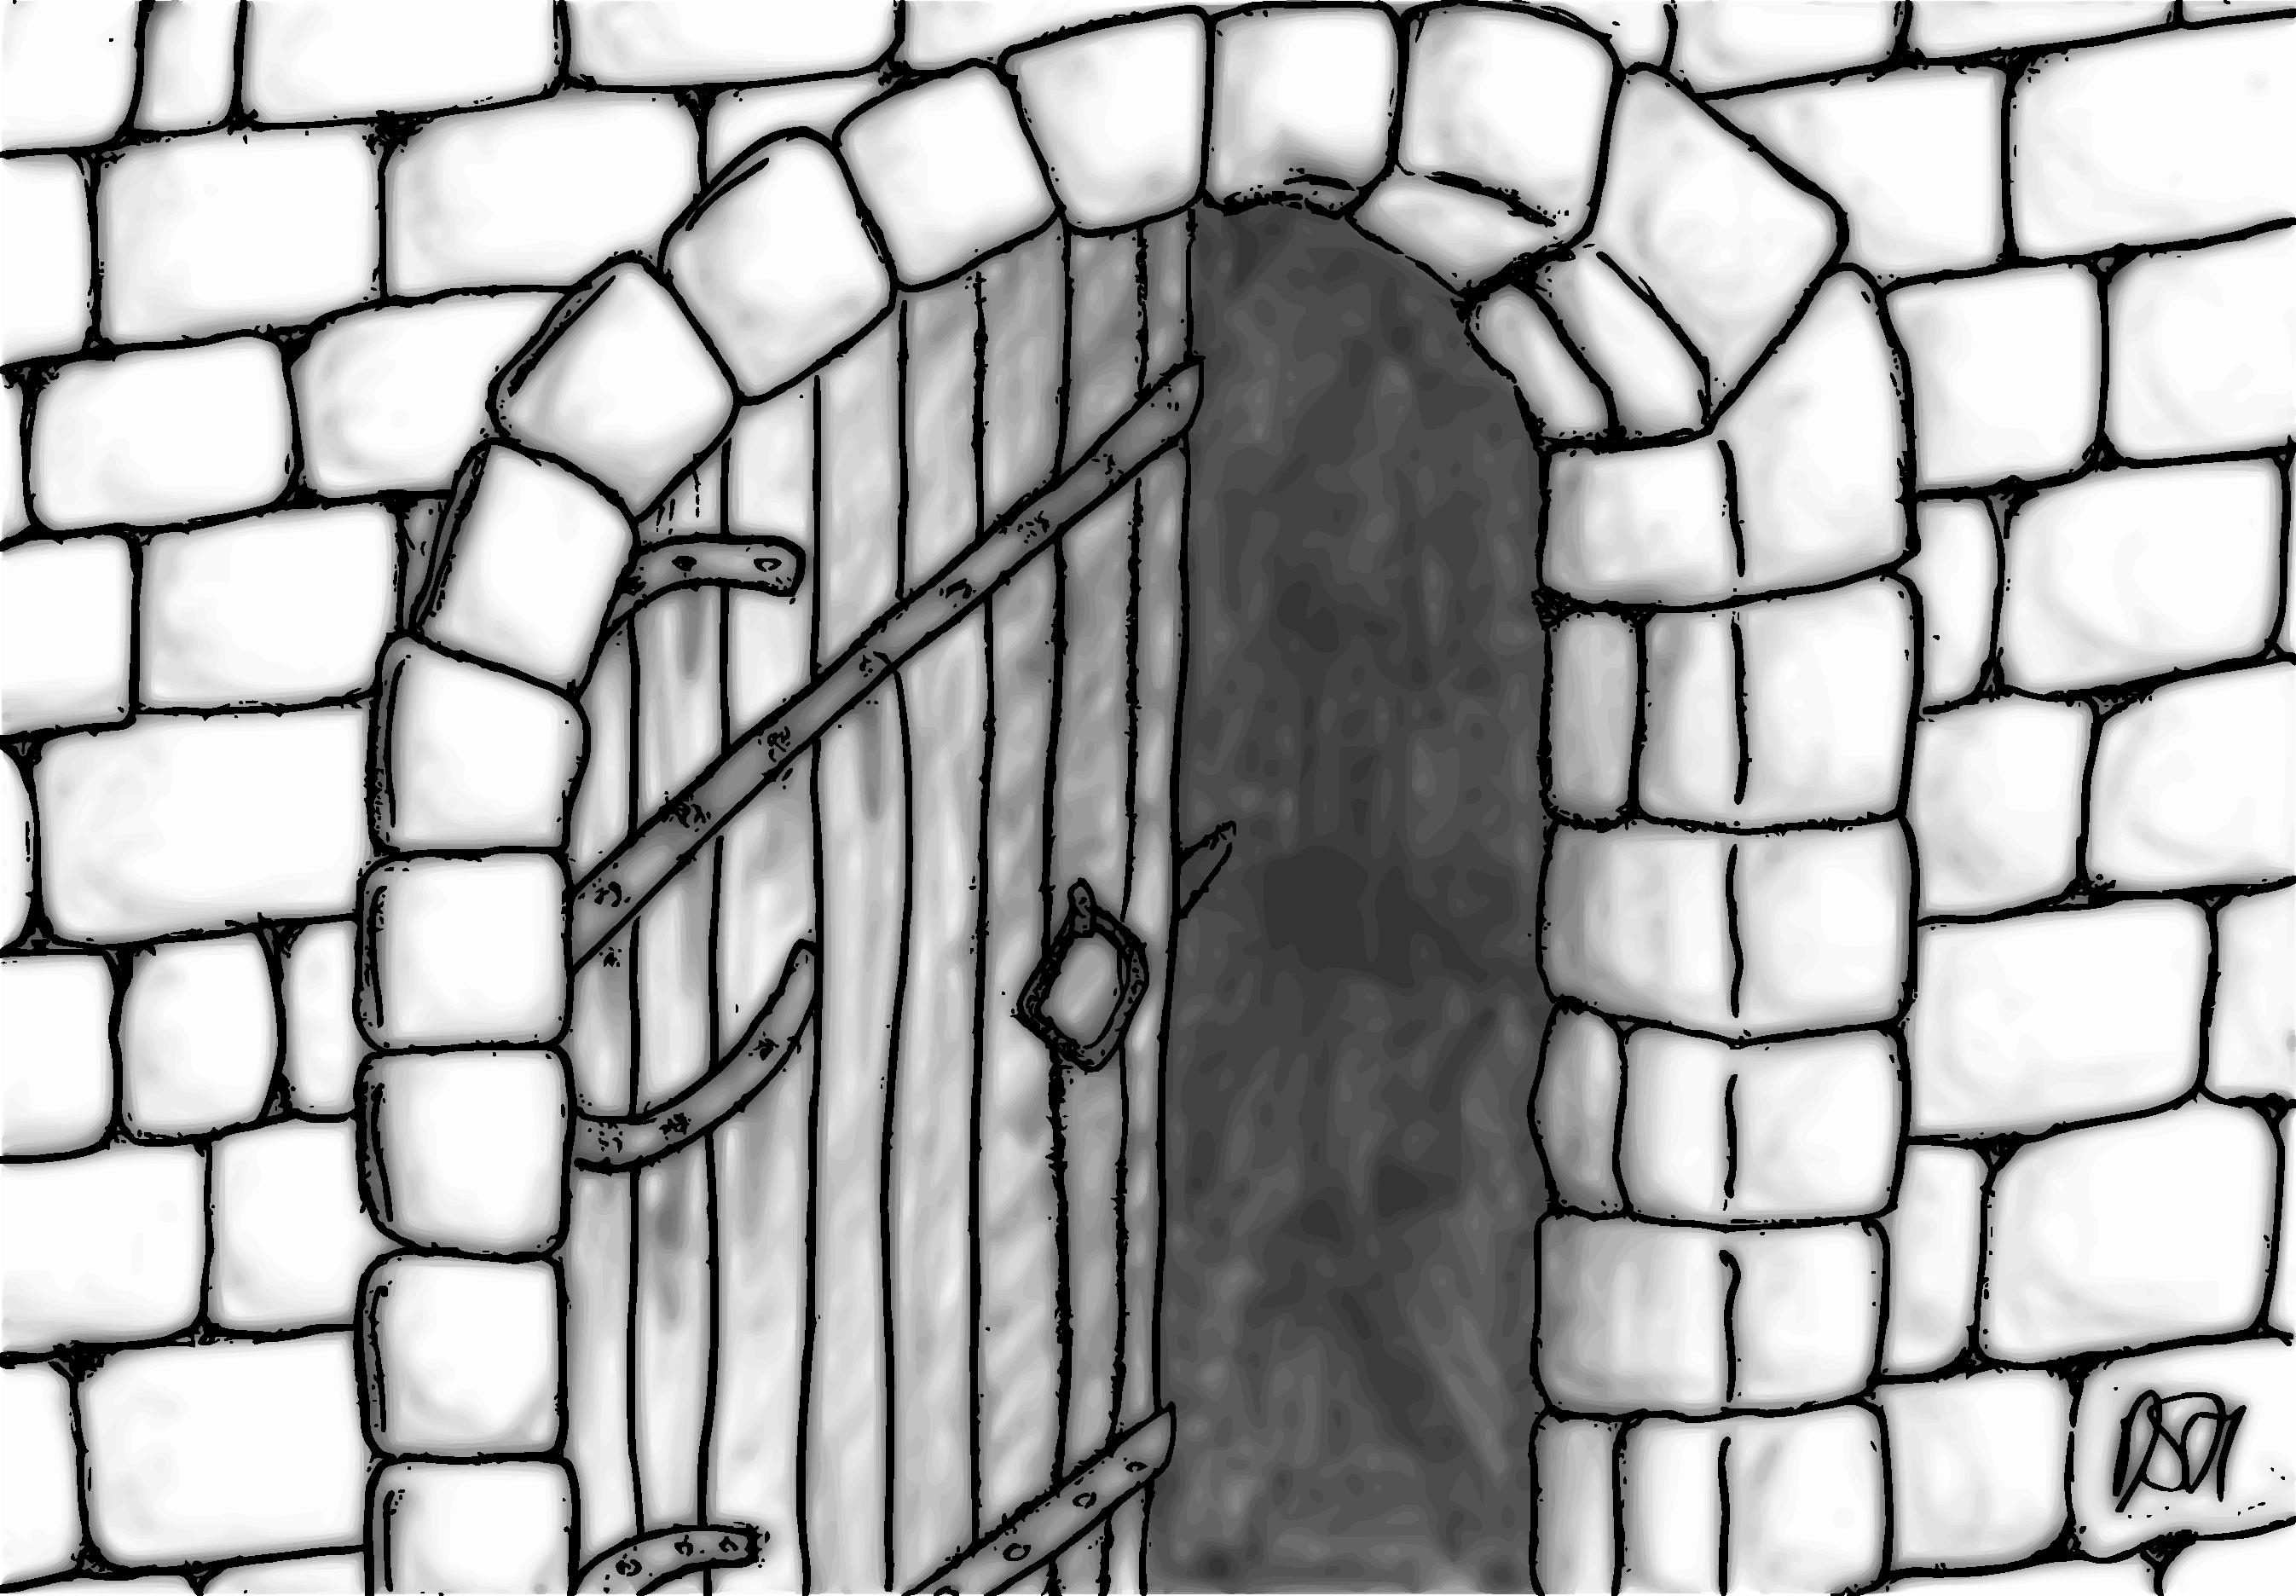
\includegraphics[width=\columnwidth]{knock.pdf}\label{knock}

\vspace{1em}

\noindent \textbf{\subsection{K}}

\noindent
\begin{minipage}{\columnwidth}

\noindent \textbf{\textit{Knock} (Universal)}

\noindent \textbf{Caster/Level:} Wizard/2

\noindent \textbf{Range:} 60 yards

\noindent \textbf{Duration:} Special

\noindent \textbf{Effective Area:} 10 square feet/level

\noindent \textbf{Components:} V

\noindent \textbf{Casting Time:} 1

\noindent \textbf{Saving Throw:} None

\end{minipage}

This spell opens stuck, barred, locked, held, or wizard locked doors, and even locked or trick-opening boxes or chests.  The spell can be used to open a secret or concealed door as long as its location is known and visible to the caster.  It can also loosen welds, shackles, or chains, provided they serve to hold the door shut.  If used to open a \textit{wizard locked} door, the spell does not remove the \textit{wizard lock} but simply suspends its functioning for one turn.  In all other cases, the door does not relock itself or become stuck again on its own.  \textit{Knock} only functions against portals that operate with a hinge mechanism and does not raise gates or similar impediments (such as a portcullis) that require a winch or rope and pulley system to open, nor does it affect ropes, vines, and the like. The effective area limits the size of the door that can be opened.  Each spell can undo up to two means of preventing egress on a single opening, so that a locked, barred and wizard locked door would require two casting of \textit{knock} to open.

The reverse, \textit{lock}, closes a known and visible door (or other portal) and locks it with up to 2 already existing physical locking mechanisms.  It cannot create a weld, magically bar a door or lower a portcullis, but it can operate locks, set bars, etc.  Up to two physical mechanisms can be set per casting.

\vspace{1em}

\noindent
\begin{minipage}{\columnwidth}

\noindent \textbf{\textit{Know Alignment} (Lesser Divination)}

\noindent \textbf{Caster/Level (Sphere):} Priest/2 (Divination), Wizard/2

\noindent \textbf{Range:} 10 yards

\noindent \textbf{Duration:} Priest---1 turn, Wizard---1 round/level

\noindent \textbf{Effective Area:} Priest---1 creature or object per round, 
Wizard---1 creature or object per 2 rounds

\noindent \textbf{Components:} V and S

\noindent \textbf{Casting Time:} 1 round

\noindent \textbf{Saving Throw:} Negate

\end{minipage}

This spell enables the caster to read a creature or item's aura, provided it has an alignment.  The caster must concentrate, standing still, for two full rounds, after casting the spell.  Creatures are allowed a save vs. spell, modified by wisdom---mental defense modifier, to avoid the effect.  Certain magical items can negate the effects of this spell.

If the caster is only able to concentrate on a subject for one round, he will only read the subject's aura in regards to law vs. chaos.  The priests' version of the spell functions as the wizard spell of the same name, except a priest is only required to stand and concentrate for 1 round to fully read the creature or item's aura.

The reverse, \textit{undetectable alignment}, blocks the aura of a single creature or item from magical detection, including the know alignment spell, for 24 hours.  If the GM wishes to allow a greater degree of intrigue and subterfuge within his game world, he may change the reverse of this spell (and any similar effects) to \textit{obscure alignment}, and permit the affected creature to radiate any alignment chosen by the caster.

\vspace{1em}

\noindent \textbf{\subsection{L}}

\noindent
\begin{minipage}{\columnwidth}

\noindent \textbf{Legend Lore (Greater Divination)}

\noindent \textbf{Caster/Level:} Wizard/6

\noindent \textbf{Range:} 0

\noindent \textbf{Duration:} Special

\noindent \textbf{Effective Area:} Special

\noindent \textbf{Components:} V, S and M

\noindent \textbf{Casting Time:} Special

\noindent \textbf{Saving Throw:} None

\end{minipage}

When more conventional research or identification methods fail or would take too much time, this spell allows the caster to learn the legends surrounding an important person, place, or item.  If the person or item is at hand, or if the caster is at the place in question, the casting time is only 1d4 turns.  If the caster has detailed information on the person, place, or item, casting requires 1d10 days, and the resulting lore is less complete and specific, but often provides enough information to help the caster find the person, place, or item, thus allowing a better legend lore result next time.  If the caster knows only rumors or hearsay, the casting time is 2d6 weeks, and the resulting lore is vague and incomplete, but often directs the caster to more detailed information, thus allowing a better legend lore result next time. 

While casting, the caster cannot engage in other than routine activities: eating, sleeping, and so forth.  When completed, the caster learns about the legends surrounding the person, place, or item.  The legends may be still current, forgotten, or even information that has never been generally known.  If the person, place, or item is not of legendary importance, the caster gains no information.  As a rule of thumb, characters of 11\textsuperscript{th} level and higher are ``legendary," as are the sorts of creatures they contend with, the major magical items they wield, and the places where they perform their key deeds.

The material components are incense burning within a rectangle made of strips of ivory, and a magical item of some kind, whether scroll, potion, wand, etc.

\vspace{1em}

\noindent
\begin{minipage}{\columnwidth}

\noindent \textbf{Leprechaun's Lamentable Belaborment (Enchantment, Evocation)}

\noindent \textbf{Caster/Level:} Wizard/5

\noindent \textbf{Range:} 10 yards

\noindent \textbf{Duration:} Special

\noindent \textbf{Effective Area:} 1 or more creatures in a 10-foot radius

\noindent \textbf{Components:} V

\noindent \textbf{Casting Time:} 5

\noindent \textbf{Saving Throw:} Special

\end{minipage}

This spell allows the caster to draw multiple subjects into an extended discourse with him, provided they have an intelligence of 3 or higher, and share a common language with the caster.  The spell effects do not begin until the round after the spell is cast, and the caster can begin speaking.  Creatures within the effective area during the round following the casting of the spell are entitled to a saving throw, specially modified by intelligence, to avoid the effects entirely.  Intelligence of 3--7 grants a $-1$ penalty, 8--10 grants no modifier, 11--14 grants a +1 bonus, and intelligence of 15 or higher grants a +2 bonus.  If this saving throw fails, the subjects immediately stop whatever else they are doing and begin to politely debate the topic with the caster, no matter how incredulous or stale his topic may be.  The actual topic of discussion is irrelevant; the words come to the caster's mind and are quickly forgotten.

The spell effect is divided into 3 distinct phases (fascination, confusion, and rage), but the caster can end the spell at the end of any phase by not continuing the discussion.  The first three rounds consist of peaceful conversation, the next three rounds are confusing babble, and the final four rounds become a heated debate.  So that the spell's duration can last up to 11--12 rounds, as long as the caster continues the discussion on the first round of each phase (the 1\textsuperscript{st}, 4\textsuperscript{th}, and 7\textsuperscript{th} rounds).  Usually, the spell's duration is a minimum of 3 rounds, however, attacking a subject of the spell, during the first or second phase, ends the effect for that creature immediately.  Once the spell is cast, it requires no concentration to maintain, and the caster is able to otherwise act normally, move, attack, cast another spell, etc.  The subjects of the spell ignore anything the caster says or does, (except attack them) that is not related to the topic they are discussing.

On the first round of each new phase, provided the caster speaks to them that round, the subjects are forced to make another saving throw, modified by intelligence.  Those failing on the 4\textsuperscript{th} round become confused and wander randomly, muttering under their breaths, for 1d10~+~2 rounds.  Those who make the save continue to discuss the topic, and make saves during the 5\textsuperscript{th} and 6\textsuperscript{th} rounds to avoid becoming confused and wandering off.  On the 7\textsuperscript{th} round, each remaining subject (those that did not wander off) must save to avoid flying into a rage, attacking the nearest other subject for 1d4~+~1 rounds.  If only one creature remains the subject of the spell and fails its save, it attacks, with a regular to hit roll, its own person.  Any creatures that successfully save against the rage effect realize they've been under the effects of an enchantment and collapse onto the ground, totally depressed for 1d4 rounds, but will snap out of it if attacked.

\vspace{1em}

\noindent
\begin{minipage}{\columnwidth}

\noindent \textbf{Leprechaun's Secret Chest (Transmutation, Conjuration)}

\noindent \textbf{Caster/Level:} Wizard/5

\noindent \textbf{Range:} Special

\noindent \textbf{Duration:} Special

\noindent \textbf{Effective Area:} One chest, 2 feet~$\times$~2 feet~$\times$~3 feet

\noindent \textbf{Components:} V, S and M

\noindent \textbf{Casting Time:} 1 turn

\noindent \textbf{Saving Throw:} None

\end{minipage}

When cast, this spell allows a specially prepared, high quality treasure chest (of at least 5,000 gp value and fashioned by a master craftsman out of the finest woods, ivories and precious metals available) to be hidden in the deep Ethereal Plane.  A perfect miniature replica, made of the same materials and valued at precisely 1\% of the full-sized chest, must also have been created before this spell is cast.  The miniature can then be used to summon the full-sized chest back from the Ether directly to the caster's location whenever needed.  Retrieving the chest ends the spell effect.  A second casting of this spell is necessary to send the chest back to the Ethereal Plane.  Each caster's set of chests is highly personalized and not even a \textit{wish} spell can allow a caster to have more than one set at any time.  The set of chests are not magical, and can be locked or magically warded just as any other treasure chest can be.  The caster must be touching the full-sized chest and holding the miniature to cast this spell.  The full-sized chest holds up to 1 cubic foot of material per caster level, regardless of its actual or apparent physical dimensions.  If living matter is placed in the chest, the spell is 75\% likely to fail.  The full-sized chest can only be recalled using its miniature.  If the miniature chest is destroyed or lost, no spell, including a \textit{wish}, can recreate it or call forth the full-sized chest.  The full-sized chest becomes lost in the Ether.  

For each continuous week spent on the Ethereal Plane, there's a cumulative 1\% chance that an ethereal creature finds the full-sized chest.  The GM must adjudicate any results from this type of chance encounter.  The chest is not anchored in one place, but even if physically stolen by a creature, it will return to the caster from anywhere on the Ethereal Plane.  The following table provides the most common results of tampering.

\noindent
\begin{tabular}{|p{.2\columnwidth}|p{.7\columnwidth}|}
\hline
1d100	& Result \\
\hline\hline
\rowcolor[gray]{.9}01-10	& Chest returns with all of its contents intact \\
11-20	& Chest returns with additional contents \\
\rowcolor[gray]{.9}21-50	& Chest returns with different contents  \\
51-80	& Chest returns with some contents missing \\
\rowcolor[gray]{.9}81-00	& Chest returns completely empty \\
\hline
\end{tabular}

When the chest is called forth from the Ethereal Plane, a window is opened for 1d6~+~6 rounds, and any creature can enter or exit through it.  If not retrieved within 60 days, there's a 5\% cumulative chance per day thereafter that the full-sized chest becomes lost in the Ether.  If the full-sized chest becomes lost in the Ether, it might only be found provided the caster is willing and able to travel to the Ethereal Plane and search for it.  Attempting to find the chest should not be an easy task, and may be next to impossible depending upon the nature of the GM's world.

\vspace{1em}

\noindent
\begin{minipage}{\columnwidth}

\noindent \textbf{Leprechaun's Secure Shelter (Transmutation, Enchantment)}

\noindent \textbf{Caster/Level:} Wizard/4

\noindent \textbf{Range:} 20 yards/level

\noindent \textbf{Duration:} 1d4~+~1 hours~+~1 hour/level

\noindent \textbf{Effective Area:} 30 square feet/level

\noindent \textbf{Components:} V, S and M

\noindent \textbf{Casting Time:} 4 turns

\noindent \textbf{Saving Throw:} None

\end{minipage}

This spell creates a small house (up to the effective area in size), solidly made of materials common to the area where it is created (usually stone, wood and/or sod).  The lodging is level, clean, and dry and otherwise appears to be a normal building with a sturdy door, two or more shuttered windows, and a fireplace, but resists all forms of attack as if it were as strong as a stone building, regardless of the material used to create it.  It can withstand winds up to 70 mph (tornado strength), but has no heating (other than the fireplace) and no cooling source other than natural insulation. 

The lodging contains simple furniture as desired by the caster; up to eight bunks with mattress and blankets, a trestle table and benches, up to four chairs or eight stools, and a writing desk.  The doors and shutters are \textit{wizard locked}, a grate of iron protects the chimney.  Additionally, the spell protects all of the possible entrances with an \textit{alarm} spell and conjures an \textit{unseen servant} to provide services for the caster and other occupants.  

The material components are crushed lime, a sprinkling of water, a square chip of stone, a few grains of sand, and several splinters of wood.  If alarm and unseen servant are to be included, their components are also required.
 
\vspace{1em}

\noindent
\begin{minipage}{\columnwidth}

\noindent \textbf{Leprechaun's Tiny Hut (Transmutation)}

\noindent \textbf{Caster/Level:} Wizard/3

\noindent \textbf{Range:} 0

\noindent \textbf{Duration:} 4 hours~+~1 hour/level

\noindent \textbf{Effective Area:} 15-foot diameter sphere

\noindent \textbf{Components:} V, S and M

\noindent \textbf{Casting Time:} 3

\noindent \textbf{Saving Throw:} None

\end{minipage}

This spell creates an immobile sphere of semi-solid force, the size of the effective area, around the caster's person, of any color he chooses.  If the spell is cast on level ground, half the sphere projects above ground and the other half below the ground.  Up to seven other man-sized creatures can enter or leave the sphere at will, but if the caster leaves it, the spell ends.  The temperature inside the sphere is a constant 70$^\circ$F, unless the exterior temperature reaches below 0$^\circ$F or above 100$^\circ$F, in which case, the interior temperature increases or decreases correspondingly.  The sphere protects against the elements (such as rain, sand and dust storms), and only hurricane force winds or greater can destroy it.

The interior of the sphere can be dimly lit or darkened on command.  The outside is opaque, and does not allow any creature to see inside, but the interior is transparent, and allows those inside to see out.  The sphere does not stop, or in any way protect anyone, from missiles, weapons, or most magical effects going in either direction, except that targets inside the sphere cannot be seen by those outside and cannot be selected individually.  A successful \textit{dispel magic} will end the spell.

The material component is a small crystal bead that shatters when the spell ends.

\vspace{1em}

\noindent
\begin{minipage}{\columnwidth}

\noindent \textbf{Leprechaun's Trap (Illusion)}

\noindent \textbf{Caster/Level:} Wizard/2

\noindent \textbf{Range:} Touch

\noindent \textbf{Duration:} Permanent

\noindent \textbf{Effective Area:} 1 object

\noindent \textbf{Components:} V, S and M

\noindent \textbf{Casting Time:} 3 rounds

\noindent \textbf{Saving Throw:} None

\end{minipage}

This spell places a false trap upon any small mechanism or device (a lock, hinge, hasp, lid etc.).  Any creature with the mechanical or magical ability to detect a trap is automatically fooled into believing the spell is a real, magical trap.  The effects are permanent until affected by a successful \textit{dispel magic} or removed (as a magical trap).  If the ``trap" is not removed and is simply ``triggered", nothing happens (since it is only an illusion), and the spell ends harmlessly.  The casting will fail, if another leprechaun's trap is within 50 feet of the caster when this spell is cast.  

The material components are a piece of iron pyrite touching the mechanism to be ``trapped", and 200 gp worth of specially prepared dust to sprinkle over it.

\vspace{1em}

\noindent
\begin{minipage}{\columnwidth}

\noindent \textbf{Levitate (Transmutation)}

\noindent \textbf{Caster/Level:} Wizard/2

\noindent \textbf{Range:} 20 yards/level

\noindent \textbf{Duration:} 1 turn/level

\noindent \textbf{Effective Area:} 1 creature or object

\noindent \textbf{Components:} V, S and M

\noindent \textbf{Casting Time:} 2

\noindent \textbf{Saving Throw:} Negate

\end{minipage}

This spell enables the subject, up to 100 pounds per caster level, to move vertically up or down at a movement value of 2 per round.  The caster controls this movement, even if cast on another creature or object, and unwilling creatures receive a saving throw vs. spell, modified by dexterity---surprise modifier, to avoid the effect.  The spell doesn't allow horizontal movement although the levitator can physically push off or grab onto objects to move laterally.

The spell requires no extra concentration.  Attacking with a ranged weapon destabilizes the levitator, applying a -1 penalty on the first such attack and a cumulative $-1$ penalty to each successive ranged attack, up to a maximum of $-5$.  Spending a full round stabilizing resets the penalty to $-1$.  Only light crossbows can be cocked and reloaded while levitating.

The material component is a small leather loop or a piece of golden wire bent into a cup shape with a long shank on one end.

\vspace{1em}

\noindent
\begin{minipage}{\columnwidth}

\noindent \textbf{Light (Transmutation)}

\noindent \textbf{Caster/Level (Sphere):} Priest/1 (Sun), Wizard/1

\noindent \textbf{Range:} Priest---120 yards, Wizard---60 yards

\noindent \textbf{Duration:} Priest- 1 hour~+~1 turn/level, Wizard- 1 turn/level

\noindent \textbf{Effective Area:} 20-foot radius globe

\noindent \textbf{Components:} Priest---V and S, Wizard---V and M

\noindent \textbf{Casting Time:} Priest---4, Wizard---1

\noindent \textbf{Saving Throw:} Special

\end{minipage}

This spell creates a glowing light, equal in strength to a torch, the size of the effective area, anywhere within range.  The caster must have a clear line of sight to the targeted area when casting this spell.  \textit{Light} can emanate from thin air, rock, metal, wood, or any other material.  The spell is stationary, unless cast on a creature or portable object.  If cast on an unwilling creature, a successful magic resistance check or a successful save vs. spell, modified by dexterity---surprise modifier, allows the creature to avoid the spell, but the light still appears in the air directly behind the creature.  If cast on a creature's eyes, a failed save indicates the creature is blinded for the duration of the spell.  Objects and creatures beyond the glow are seen as vague, shadowy forms. 

\textit{Light} taken into an existing magical darkness will be blotted out (or vice versa), however, casting light onto an existing magical darkness (or vice versa) negates both effects until one effect's or the other's duration ends, at which time, the effect with the longer duration reappears.  The caster can end the spell with a command word.  \textit{Light} spells cannot stack, so that overlapping effective areas do not get brighter.

The material component is a firefly or piece of phosphorescent moss.

The priests' version of this spell functions as the wizards' spell of the same name, except it is reversible.  The reverse, \textit{darkness}, brings pitch darkness to the effective area, with half the spell's normal duration.  A mundane or magical light source must be as bright as full daylight in order to be seen within the effective area.  

\vspace{1em}

\noindent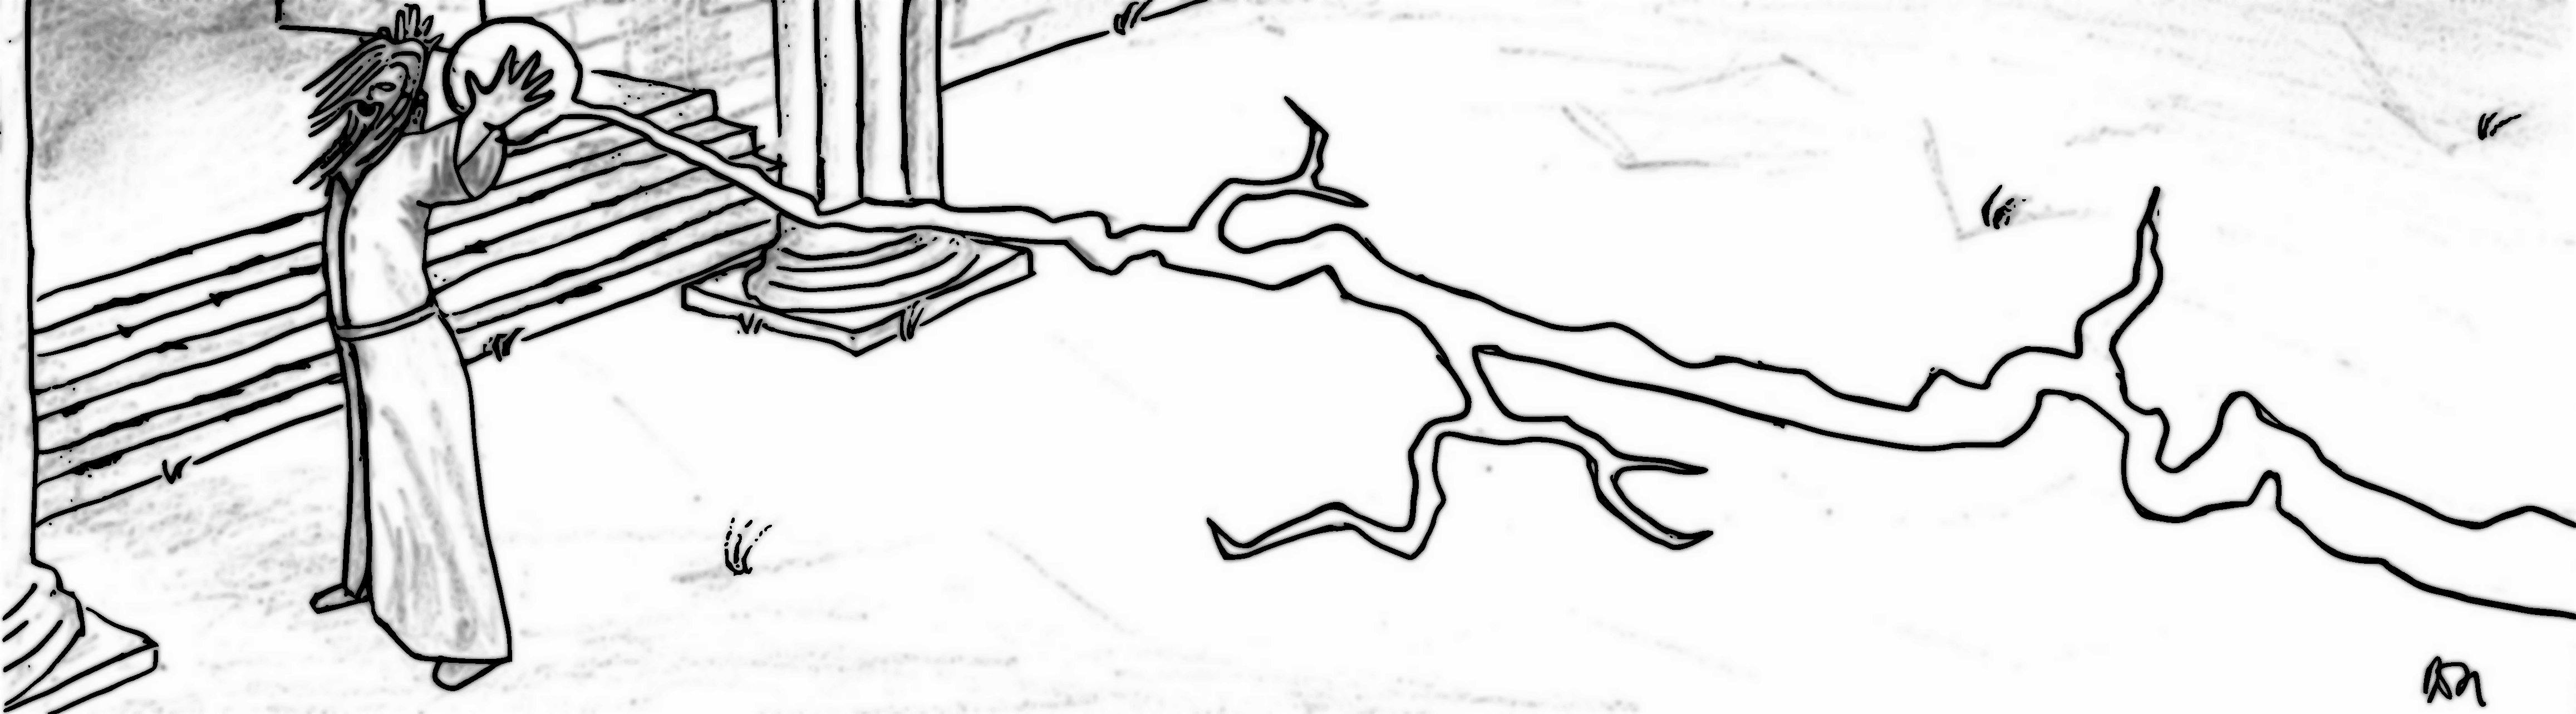
\includegraphics[width=\columnwidth]{lightningbolt.pdf}\label{lightningbolt}

\vspace{1em}

\noindent
\begin{minipage}{\columnwidth}

\noindent \textbf{Lightning Bolt (Evocation)}

\noindent \textbf{Caster/Level:} Wizard/3

\noindent \textbf{Range:} 40 yards~+~10 yards/level

\noindent \textbf{Duration:} Instantaneous

\noindent \textbf{Effective Area:} Special

\noindent \textbf{Components:} V, S and M

\noindent \textbf{Casting Time:} 3

\noindent \textbf{Saving Throw:} Half

\end{minipage}

This spell creates a stroke of electricity beginning at a point within the spell's range and extending in a straight line outward directly away from the caster, inflicting 1d6 points of damage per caster level (up to a maximum of 10d6) to all creatures in its path.  A successful save vs. spell, modified by dexterity-surprise modifier, reduces the damage by half.  The spell's effective area can be either a forked bolt, 10 feet wide and 40 feet long or a single bolt 5 feet wide and 80 feet long.  

The electricity in the effective area can set fire to combustibles, melt soft and precious metals, and is powerful enough to do minor structural damage, penetrating and continuing beyond 1 inch of wood (destroying most standard doors) or a $^1$/$_2$ inch of stone per caster level (up to a maximum of 1 foot of wood or $^1$/$_2$ foot of stone), unless the item successfully saves against the effect.  If the bolt strikes an impassable barrier (or a barrier makes its save), the energy reflects off the barrier at an angle equal to the angle it struck the barrier (like a billiard ball, or reflected light), until its maximum effective area is achieved.  A bolt shot straight into a barrier will reflect directly back at the caster.  Creatures struck more than once from a reflected bolt, must make a save each time, but do not take damage more than once.  If every saving throw is successful, reduce damage by half, but if even one saving throw is failed, full damage is inflicted.

The material components are a bit of fur and an amber, crystal, or glass rod.

\vspace{1em}

\noindent
\begin{minipage}{\columnwidth}

\noindent \textbf{Limited Wish (Conjuration, Evocation)}

\noindent \textbf{Caster/Level:} Wizard/7

\noindent \textbf{Range:} Unlimited

\noindent \textbf{Duration:} Special

\noindent \textbf{Effective Area:} Special

\noindent \textbf{Components:} V and Special

\noindent \textbf{Casting Time:} Special

\noindent \textbf{Saving Throw:} Special

\end{minipage}

This spell is an extremely powerful spell that can require extra attention from the GM and player alike, but in its simplest form, this spell allows the caster to create nearly any type of known magical effect, of equal or lesser level.

A \textit{limited wish} can duplicate any wizard spell of 7\textsuperscript{th} level or lower, provided the spell is from a school of magic allowed to the caster, and any wizard spell of 5\textsuperscript{th} level or lower, even from a prohibited school, or duplicate any priest spell of 5\textsuperscript{th} level or lower, provided the spell is from a school of magic allowed to the caster, and any priest spell of 4\textsuperscript{th} level or lower, even from a prohibited school.  Using this spell to duplicate another spell must follow all rules for the spell being duplicated.  Subjects are allowed the same saving throws and magic resistance as normal.  The caster is subject to the same risks and rewards as if they had cast the actual spell, with the following exceptions.  Any variable that can benefit the caster will be as if the maximum was rolled and if used to duplicate a spell with a material component that costs less than 1,000 gp, the caster does not need to provide the component.  All verbal and somatic components must be used and the casting time is equal to that of the duplicated spell.

Another form of the spell can be used literally as a limited form of a \textit{wish}, fulfilling any function of the \textit{wish} spell, and within the same constraints, but only for a limited amount of time (See the \textit{wish} spell).  A \textit{limited wish} is able to undo or modify the harmful effects of the same spells as can be affected by a \textit{wish} spell. If a \textit{wish} spell can permanently affect or undo a magical effect, a \textit{limited wish} can affect or undo the effect for a limited time. The GM must determine the limited duration, but a rule of thumb may be (1d6~+~1 weeks)~+~1 week per caster level.  The casting time for this form is about 1--3 rounds, depending on the complexity of the \textit{wish}.

And finally, the caster can produce any other effect whose power level is in line with the above effects, such as a ball of frost that inflicts cold damage, but otherwise duplicates a \textit{fireball} spell, or a single creature may be granted a +7 bonus to hit on its next attack or suffer up to a $-7$ penalty on its next saving throw, etc.  The caster is allowed to be creative when using this form of the limited wish, and with the GM's consent, the spell could be used as an aid in spell research for new spells of 6\textsuperscript{th} level or lower.  The casting time for this form can vary greatly.

Casting this spell ages a caster one year if his venerable age is 150 years or less, two years if his venerable age is between 151 and 250 years, three years if his venerable age is between 251 and 350 years, etc.

\vspace{1em}

\noindent
\begin{minipage}{\columnwidth}

\noindent \textbf{Live Oak (Enchantment)}

\noindent \textbf{Caster/Level (Sphere):} Priest/6 (Plant)

\noindent \textbf{Range:} Touch

\noindent \textbf{Duration:} 1 day/level

\noindent \textbf{Effective Area:} 1 tree

\noindent \textbf{Components:} V, S and M

\noindent \textbf{Casting Time:} 1 turn

\noindent \textbf{Saving Throw:} None

\end{minipage}

This spell enchants a healthy tree to guard and protect a place or item of the caster's choice.  The spell affects a tree that is within 10 feet of the caster's home, within a place sacred to the caster, or within 100 yards of an item the caster wants to guard.  The caster cannot have more than one live oak spell in effect concurrently.

The GM is called upon to note the locations and sizes of trees in the area to be protected.  The selected tree can be small, medium, or large in size, depending upon the caster's choice of available trees.  

An activation clause consisting of as many as one word per caster level is given at casting time, including what action to take and passwords or special items used to bypass it.  For example, an 11\textsuperscript{th} level caster can form an 11-word activation clause; such as ``Attack all creatures who approach the obelisk without first saying `friend'."  The enchanted tree is treated as a treant of equivalent size, with an AC 0 and 2 attacks per round, but a movement value of only 3.

\noindent
\begin{tabular}{|p{.2\columnwidth}|p{.2\columnwidth}|p{.2\columnwidth}|p{.2\columnwidth}|}
\hline
Size	& Height	& HD	& Damage \\
\hline\hline
\rowcolor[gray]{.9}Small	& 12'--14'	& 8	& 2d8 \\
Medium	& 16'--19'	& 10	& 3d6 \\
\rowcolor[gray]{.9}Large	& 20'--23'+	& 12	& 4d6 \\
\hline
\end{tabular}

A \textit{detect magic} spell or similar magic will show strong magic radiating from the tree.  If a successful \textit{dispel magic} is cast, the spell ends immediately, and the tree will root itself at its current location.  The caster may release it from the spell effects at any time, whereupon it returns to its original spot before taking root.  Damaged trees can be healed with the plant growth spell, restoring 3d4 points of damage, but the spell cannot be used to increase the size or maximum hit points of an already enchanted tree.
 
The material component is the caster's holy or unholy symbol.

\vspace{1em}

\noindent
\begin{minipage}{\columnwidth}

\noindent \textbf{Locate Animals or Plants (Lesser Divination)}

\noindent \textbf{Caster/Level (Sphere):} Priest/1 (Divination (Animal, Plant))

\noindent \textbf{Range:} 100 yards~+~20 yards/level

\noindent \textbf{Duration:} 1 round/level

\noindent \textbf{Effective Area:} 20-foot~$\times$~20-yards/level path

\noindent \textbf{Components:} V, S and M

\noindent \textbf{Casting Time:} 1 round

\noindent \textbf{Saving Throw:} None

\end{minipage}

This spell allows the caster to know whether any one type of animal or plant, which he thinks of, is within the spell's range, determining its direction, distance and approximate numbers.  The caster can only detect subjects directly in front of him in a straight path, but he can change direction once each round of the spell's duration.

The GM must adjudicate the results of this spell carefully.  However, after taking the surrounding terrain and climate into account, some general guidelines can be followed.  Many herbs grow only in the temperate zones, while many spices grow only in the tropics.  Common local plants and animals are up to 50\% likely to be present, somewhere in a radius around the caster, uncommon ones up to 30\% likely, rare up to 15\% likely, and very rare is up to 5\% likely to be present, somewhere within range of the caster's immediate area, but not necessarily in the direction he is facing.  Many of the exotic plants and animals needed for material components or research are considered very rare or rare, at best.

The material component is the caster's holy or unholy symbol.

\vspace{1em}

\noindent
\begin{minipage}{\columnwidth}

\noindent \textbf{\textit{Locate Object} (Lesser Divination)}

\noindent \textbf{Caster/Level (Sphere):} Priest/3 (Divination), Wizard/2

\noindent \textbf{Range:} Priest---60 yards~+~10 yards/level, Wizard---20 yards/level

\noindent \textbf{Duration:} 1 round/level

\noindent \textbf{Effective Area:} 1 item

\noindent \textbf{Components:} V, S and M

\noindent \textbf{Casting Time:} Priest---1 turn, Wizard---2

\noindent \textbf{Saving Throw:} None

\end{minipage}

This spell can assist the caster when he is searching for either a specific, known item or a non-specific, general item.  When the caster searches for a general item (swords, gems, stairs, elevators, etc.), he learns the direction in which lies the nearest one of its kind (if any), within range.  The caster must have seen or otherwise physically handled a specific item, in order to search for them with this spell.  A thin coating of lead blocks the spell.  The caster cannot use this spell to search for a creature.

The material component is a forked twig.

The reverse, \textit{obscure object}, hides an object from being located by spell, \textit{crystal ball}, or similar means for eight hours.  The object to be obscured must be touched, and the caster cannot obscure a creature with this spell. 

The material component for the reverse is a chameleon's skin.

The priests' version of the spell functions as the wizards' spell of the same name, except that the material component, for both the spell and the reverse, is a piece of lodestone.

\vspace{1em}

\noindent
\begin{minipage}{\columnwidth}

\noindent \textbf{\textit{Lower Water} (Transmutation)}

\noindent \textbf{Caster/Level (Sphere):} Priest/4 (Elemental (Water)), Wizard/6

\noindent \textbf{Range:} Priest- 12o yards, Wizard- 80 yards

\noindent \textbf{Duration:} Priest- 1 turn/level, Wizard- 5 rounds/level

\noindent \textbf{Effective Area:} 10-foot~$\times$~10-foot by 2-foot deep/level

\noindent \textbf{Components:} V, S and M

\noindent \textbf{Casting Time:} 1 turn

\noindent \textbf{Saving Throw:} None

\end{minipage}

This spell drains away water or similar liquids, up to the effective area, but the liquid's final depth cannot be less than 1-inch deep.  When cast on a deep ocean, sea or large lake, this spell creates a whirlpool, trapping swimmers, boats, ships, etc.  Those trapped in a whirlpool will not be able to leave the effective area under their own power, and are at risk of capsizing and being sucked into the center of the swirling water.  If this spell is cast on a water elemental or other water-based creature, the creature is affected as if a slow spell had been cast on it (no save allowed).  At the spell duration's end, the water returns to its previous level.  The use of this spell negates its reverse.

The material component of lower water is a vial of dust.

The reverse, \textit{raise water}, increases the volume of a body of liquids by the effective area, up to the maximum natural level (such as flash flood or high tide level).  Ships, boats, swimmers, etc. are unable to stay within the effective area and are immediately forced outward and down the sides of the huge stationary ``wave" that the reverse creates.  If the effective area includes a riverbank, beach, or other land, the water can spill over, possibly flooding or washing away docks, fords, dams, roads and bridges and floating beached or grounded ships.  At the duration's end, the water returns to its previous level.  The GM must determine the exact effects of the flooding and receding waters.  The use of the reverse negates \textit{lower water}.

The material component of raise water is a vial of water.

The priests' version of this spell functions as the wizards' spell of the same name, except that in addition to water or dust, the caster requires his holy or unholy symbol.

\vspace{1em}

\noindent \textbf{\subsection{M}}

\noindent
\begin{minipage}{\columnwidth}

\noindent \textbf{Mage's Disjunction (Transmutation, Enchantment)}

\noindent \textbf{Caster/Level:} Wizard/9

\noindent \textbf{Range:} 0

\noindent \textbf{Duration:} Instantaneous

\noindent \textbf{Effective Area:} 30-foot radius

\noindent \textbf{Components:} V

\noindent \textbf{Casting Time:} 9

\noindent \textbf{Saving Throw:} Special

\end{minipage}

This spell is an extremely powerful variant of \textit{dispel magic}, allowing the caster to attempt to immediately disrupt spell casting and permanently dispel all magic effects and magical items, within the effective area.  This spell functions as if multiple \textit{dispel magic} were cast in an area, with the additional ability to permanently destroy magical items and disrupt spell casting all at once.  In addition, the spell ignores spell casting, magical items and magic effects of the caster, and of any single creature he is touching.  

All spells being cast within the effective area are automatically, and immediately disrupted.  Within the effective area, all spells with duration in effect, including permanent durations (no matter how many), are subject to \textit{dispel magic}, and all magical items are subject to \textit{dispel magic} (as if they were each targeted), but if the check fails, an item permanently loses all of its magic (Refer to \textit{Dispel Magic}).  

This spell is so powerful that there is a 1\% chance per caster level to affect artifacts, relics, and anti-magic shells, as well.  If an anti-magic shell makes its save, it protects the items within it.  If an artifact or relic is destroyed, the caster must immediately save vs. spell with a $-4$ penalty, or permanently lose all spell casting abilities.  In addition, these items are always associated with powerful being(s) (usually of extra-planar origin), who are 95\% likely to notice the item's destruction.  The GM must determine how long it takes for the being to notice, and the being's reactions upon hearing the news. 

\vspace{1em}

\noindent
\begin{minipage}{\columnwidth}

\noindent \textbf{Mage's Faithful Hound (Conjuration)}

\noindent \textbf{Caster/Level:} Wizard/5

\noindent \textbf{Range:} 10 yards

\noindent \textbf{Duration:} Special

\noindent \textbf{Effective Area:} Special

\noindent \textbf{Components:} V, S and M

\noindent \textbf{Casting Time:} 5

\noindent \textbf{Saving Throw:} None

\end{minipage}

This spell summons a phantom watchdog that only the caster can see.  The dog stands in a fixed location and guards any open space or portal, barking loudly whenever any creature larger than a rabbit or cat comes within the spell's range of the location it is standing.  It can detect invisible and ethereal creatures and is not fooled by illusions unless they're quasi-real.  

If an intruder continues past the invisible, barking dog, and into the guarded area, the dog is able to move, up to the spell's range, from its fixed location and attack the intruder as a 10 HD monster, inflicting 3d6 points of damage with its bite.  Its bite is considered as if it were a +3 magical weapon for purposes of hitting a creature requiring magic weapons to hit.  The hound is immune to all attack forms, but a successful \textit{dispel magic} will destroy it.  The spell lasts 1 hour plus $^1$/$_2$ hour per caster level until an intruder is attacked, whereupon the duration is reduced to only one round per caster level.  If the caster moves more than 30 yards away from the hound, the spell ends.  

The material components are a tiny silver whistle, a piece of bone, and a thread.

\vspace{1em}

\noindent
\begin{minipage}{\columnwidth}

\noindent \textbf{Mage's Lucubration (Transmutation)}

\noindent \textbf{Caster/Level:} Wizard/6

\noindent \textbf{Range:} 0

\noindent \textbf{Duration:} Instantaneous

\noindent \textbf{Effective Area:} The caster

\noindent \textbf{Components:} V and S

\noindent \textbf{Casting Time:} 1

\noindent \textbf{Saving Throw:} None

\end{minipage}

This spell is a mnemonic enhancer that allows the caster to recall a single 1\textsuperscript{st} through 5\textsuperscript{th} level spell, which he has cast within the last 24 hours.  Any material components needed to cast the recalled spell must be available before it can be cast again.

\vspace{1em}

\noindent
\begin{minipage}{\columnwidth}

\noindent \textbf{Mage's Magnificent Mansion (Transmutation, Conjuration)}

\noindent \textbf{Caster/Level:} Wizard/7

\noindent \textbf{Range:} 10 yards

\noindent \textbf{Duration:} 1 hour/level

\noindent \textbf{Effective Area:} 300 square feet/level

\noindent \textbf{Components:} V, S and M

\noindent \textbf{Casting Time:} 7 rounds

\noindent \textbf{Saving Throw:} None

\end{minipage}

This spell creates a mansion within Non-dimensional Space that can only be entered through a faint, shimmering entryway (4~$\times$~8 feet) located on the plane where the spell was cast.  The portal can be opened or closed, allowing entrance and egress, at the caster's desire.  When closed, it is invisible to all but the caster.  The interior of the mansion consists of a lavishly furnished entrance hall leading to multiple rooms, up to the size of the effective area.  Semi-transparent, liveried servants wait on everyone.  Its non-dimensional nature means the weather does not affect the interior of the mansion, and vice versa.  The environment is comfortable, and creatures can rest and relax inside.  There's enough food to feed a 9-course formal feast to a dozen man-sized creatures per caster level.  However, the food is only quasi-real.  Those that eat the food are satisfied until they leave, at which time, the effects disappear, and they must eat real food immediately or begin to starve.  Any object taken out of the mansion immediately ceases to exist.

This spell can be combined with illusions, or even a mundane building, to disguise the opening into Non-dimensional Space.  The GM may allow the caster to design the interior, within the scope of the effective area, to suit their specific needs.

The material components are a miniature portal carved from ivory, a small piece of polished marble, and a tiny silver spoon.

\vspace{1em}

\noindent
\begin{minipage}{\columnwidth}

\noindent \textbf{Mage's Sword (Evocation)}

\noindent \textbf{Caster/Level:} Wizard/7

\noindent \textbf{Range:} 30 yards

\noindent \textbf{Duration:} 1 round/level

\noindent \textbf{Effective Area:} Special

\noindent \textbf{Components:} V, S and M

\noindent \textbf{Casting Time:} 7

\noindent \textbf{Saving Throw:} None

\end{minipage}

This spell creates a shimmering, sword-like force field that floats in the air and moves as the caster mentally directs.  The caster can move but must otherwise concentrate to mentally command the sword.  It can move freely within the spell's range and attacks as a fighter of half the caster level, but always hits on a natural roll of 19--20, is treated as a +3 weapon for purposes of hitting a creature requiring magic weapons to hit, and can hit ethereal, astral, or out-of-phase creatures, inflicting 5d4 points of damage to man-sized and smaller creatures or 5d6 points to large-sized creatures.  The sword remains for the duration, unless the caster stops concentrating, it moves beyond range, or a \textit{dispel magic} is cast successfully.

The material component is a miniature platinum sword with a grip and pommel of copper and zinc, costing at least 500 gp.

\vspace{1em}

\noindent
\begin{minipage}{\columnwidth}

\noindent \textbf{Magical Aura (Illusion)}

\noindent \textbf{Caster/Level:} Wizard/1

\noindent \textbf{Range:} Touch

\noindent \textbf{Duration:} 1 day/level

\noindent \textbf{Effective Area:} Special

\noindent \textbf{Components:} V, S and M

\noindent \textbf{Casting Time:} 1 round

\noindent \textbf{Saving Throw:} Special

\end{minipage}

This spell masks the actual magical aura of an item of up to five pounds per caster level and bestows a false magical aura upon it.  The caster must specify intensity and school, and optionally, can provide sphere.  If \textit{detect magic} or similar method is used, the item gives off the aura as specified by the caster at the time of casting.  Artifacts, relics and other powerful magical items (as may be specified by the GM) are immune to the effects of this spell.

If the item is investigated with an identify spell or similar divination, there's a 50\% chance for the investigator to detect the true aura behind the false.  Otherwise, the false aura becomes fixed, and that investigator cannot determine the original aura.  Another investigator may try, of course.  No other information can be gained regarding the item, unless the true aura is first determined.  

The spell lasts for the duration, or until a successful \textit{dispel magic} is targeted at the item, but if the false aura is not present and the item is genuinely magical, \textit{dispel magic} could temporarily disable the item.

The material component is a small square of silk, which is passed over the item.

\vspace{1em}

\noindent
\begin{minipage}{\columnwidth}

\noindent \textbf{Magic Font (Greater Divination)}

\noindent \textbf{Caster/Level (Sphere):} Priest/5 (Divination)

\noindent \textbf{Range:} Touch

\noindent \textbf{Duration:} Special

\noindent \textbf{Effective Area:} Special

\noindent \textbf{Components:} V, S and M

\noindent \textbf{Casting Time:} 1 hour

\noindent \textbf{Saving Throw:} None

\end{minipage}

This spell allows a caster (who is in good standing with his faith) to enchant a sacred, but mundane, basin of holy or unholy water to act like a \textit{crystal ball}.  The spell's duration is equal to one round per vial of holy or unholy water poured into the font, up to a maximum of 1 hour.

The material components are the caster's holy or unholy symbol and font, and 1-60 vials of holy or unholy water.  The vials of holy or unholy water are consumed by the spell.

\vspace{1em}

\noindent
\begin{minipage}{\columnwidth}

\noindent \textbf{Magic Jar (Necromancy)}

\noindent \textbf{Caster/Level:} Wizard/5

\noindent \textbf{Range:} 10 yards/level

\noindent \textbf{Duration:} Special

\noindent \textbf{Effective Area:} 1 creature

\noindent \textbf{Components:} V, S and M

\noindent \textbf{Casting Time:} 1 round

\noindent \textbf{Saving Throw:} Special

\end{minipage}

This spell allows the caster to abandon his body (leaving it in suspended animation (Refer to Temporal Stasis)) and transfer his life force into a special personalized vessel, provided it's within range, and from there he can attempt to swap his life force with that of another creature.  The vessel must be a flawless gem or crystal, cut by a master gem-cutter, and cost at least 500 gp.  It is otherwise a mundane gem and only radiates magic while this spell is in effect.  If checked with appropriate magic, the vessel also radiates the same alignment as that of the life force inside it, if any.

While a life force is in the vessel, it can sense any other life force on the same plane and within range, but does not age, nor does it feel the need to eat, breathe or sleep.  The trapped creature (whether the caster or victim) learns whether the life force is positive (living) or negative (undead), but the type of creature and its location are not known.  Long-term entrapment inside the vessel may cause long-term or permanent insanity.  The GM must adjudicate the results of long-term entrapment.

Once a life force is detected, the caster can spend 1 round attempting to take over its body.  If the targeted creature is under the effects of a protection from evil (or good) or similar magic, the attempted possession automatically fails.  Otherwise, the creature must save vs. spell, modified by a special modifier, based on it's intelligence~+~wisdom subtracted from the caster's intelligence~+~wisdom.  If a targeted creature's wisdom cannot be determined or is less than its HD, substitute the creature's HD.  If the targeted creature's combined total is higher than the caster's, it results in a bonus to the creature's save.  

\noindent
\begin{tabular}{|p{.5\columnwidth}|p{.4\columnwidth}|}
\hline
Difference	& Modifier \\
\hline\hline
\rowcolor[gray]{.9}$-9$ or less	& +4 \\
$-8$ to $-6$	& +3 \\
\rowcolor[gray]{.9}$-5$ to $-3$	& +2 \\
$-2$ to 0	& +1 \\
\rowcolor[gray]{.9}+1 to +4	& +0 \\
+5 to +8	& $-1$ \\
\rowcolor[gray]{.9}+9 to +12	& $-2$ \\
+13 or more	& $-3$ \\
\hline
\end{tabular}

If a group of creatures approach the caster's vessel, he senses their number and a difference between them of four or more levels or HD, but cannot otherwise determine exactly who or what the life forces belong to.  For example: if three 12\textsuperscript{th} level fighters enter the range with a stone giant, 2 gnolls and 4 orcs, the caster detects 4 stronger positive and 6 weaker positive life forces.  In a case like this, the caster can choose to attack one of the stronger or one of the weaker creatures, but the GM determines randomly which specific creature is targeted (in this case, with either 1d4 or 1d6).  

If the creature's saving throw is successful, the caster remains in the vessel until he can attack again, but if the creature fails the save, the caster takes over its body and forces its life force into the vessel.  The caster gains the creature's strength, dexterity and constitution scores, as well as hit points and innate magical powers, but remembers only basic knowledge on an instinctual level, not life-defining events, learned abilities, languages, or spells.  The caster retains his attributes of intelligence, wisdom and charisma, as well as attack rolls, saving throws, class level, learned abilities, and spells.  The caster must have access to his material components, and generally speaking, he must take over a humanoid body in order to cast spells, but the GM may make the rare exception.  If the new form is radically different from the caster's old form, the GM may also assign penalties until the caster becomes accustomed to the new form. 

At any time the caster is within range, he can spend one round to shift from the possessed body back to the vessel, which returns the creature's life force back to its body.  The spell's duration is permanent until the caster makes a final shift from the vessel back into his original body.

If \textit{dispel magic} is targeted on the possessed body or the vessel, there's a 50\% chance of success, +/- 5\% per difference in caster level of the creature who cast \textit{dispel magic}.  If a \textit{dispel magic} is successfully cast on the vessel or the possessed body, and the possessed body and vessel are within range of each other, the creature returns to his body, while the caster returns to the vessel and is trapped inside for 1d4 rounds~+~1 round per level of the caster who cast \textit{dispel magic}.  If the possessed body is not in range of the vessel, the caster dies, but the creature's life force remains trapped inside the vessel and its body enters suspended animation.  In this case, a second \textit{dispel magic} targeted on the vessel reunites the life force inside with its own body or that of the caster, when one or the other is within range (the closest living body is taken).  If neither body is in range, the life force dies.  If the caster's body is taken, it is treated as possessed and subject to \textit{dispel magic}, and it would be in the creature's best interest to return to its own body as soon as possible.  If the vessel and both bodies are within range and still living, and a \textit{dispel magic} is successfully cast on the vessel, the caster and creature return to their original bodies, ending the spell, but if their respective bodies are outside the range or dead, they die.  If a possessed body is killed, the caster returns to the vessel (if within range), and the creature's life force dies.  If the possessed body is killed while the vessel is outside of range, the caster's life force also dies.  Since its body was killed, the trapped life force in the vessel is released to die, however, has a 50\% chance to possess the caster's body if it is in range of the vessel.  If the caster's body is killed, his life force may still live, either within the vessel or in a possessed body.   Raise dead, resurrection or similar magic must be used to bring those killed by this spell (whether caster or creature) back to life, however, if the vessel is destroyed while containing the caster's life force, the caster is irrevocably slain.  If the caster's body is killed and raised while his life force is in the vessel or in a possessed body, his life force is instantly returned to his original body, ending the spell.  However, other entrapped creatures are not irrevocably slain, as their life force is not an integral part of the spell as is the caster's.

The material component is the gem or crystal to serve as the vessel, which is not destroyed during the casting.  The caster can have the stone set in jewelry, a statuette, etc., or it can remain unset.  Once the caster has possessed a body, the wisest course of action is to keep this gem with him at all times.  If this vessel is destroyed while the caster possesses another body, he will be unable to return to his own body and may be instantly killed if targeted by \textit{dispel magic}.

\vspace{1em}

\noindent
\begin{minipage}{\columnwidth}

\noindent \textbf{Magic Mirror (Enchantment, Greater Divination)}

\noindent \textbf{Caster/Level:} Wizard/4

\noindent \textbf{Range:} Touch

\noindent \textbf{Duration:} 1 round/level

\noindent \textbf{Effective Area:} Special

\noindent \textbf{Components:} V, S and M

\noindent \textbf{Casting Time:} 1 hour

\noindent \textbf{Saving Throw:} None

\end{minipage}

This spell enchants a mundane mirror, which has been crafted by a master silversmith from finely wrought and highly polished silver, and costing at least 1,000 gp, into a scrying device that functions as a \textit{crystal ball} for the duration of the spell.  

\textit{Comprehend languages}, \textit{read magic}, \textit{tongues}, and \textit{infravision} can be cast through the mirror, while \textit{detect magic}, \textit{detect good/evil}, and \textit{message} have a 5\% chance per caster level of functioning when cast through the mirror.

In addition to the mirror (which is not destroyed), an eye of a hawk, an eagle, or a roc, and a small bit of each, nitric acid, copper, and zinc, are consumed upon casting.

\vspace{1em}

\noindent
\begin{minipage}{\columnwidth}

\noindent \textbf{Magic Missile (Evocation)}

\noindent \textbf{Caster/Level:} Wizard/1

\noindent \textbf{Range:} 60 yards~+~10 yards/level

\noindent \textbf{Duration:} Instantaneous

\noindent \textbf{Effective Area:} 1-5 creatures

\noindent \textbf{Components:} V and S

\noindent \textbf{Casting Time:} 1

\noindent \textbf{Saving Throw:} None

\end{minipage}

This spell allows the caster to fire one or more missiles of magical energy from his fingertips and unerringly strike a targeted creature.  A creature must be within range, in sight, and under less than 90\% cover or concealment, to be targeted.  Specific body parts of a creature cannot be targeted.  The missiles cause no structural damage, but each inflicts 1d4~+~1 points of damage to most creatures.  The caster can fire an additional missile every two levels of experience up to a maximum of five missiles at 9\textsuperscript{th} level.  Multiple missiles can strike a single creature or be split against several creatures.

\vspace{1em}

\noindent
\begin{minipage}{\columnwidth}

\noindent \textbf{Magic Mouth (Transmutation)}

\noindent \textbf{Caster/Level:} Wizard/2

\noindent \textbf{Range:} 10 yards

\noindent \textbf{Duration:} Permanent until triggered

\noindent \textbf{Effective Area:} 1 object

\noindent \textbf{Components:} V, S and M

\noindent \textbf{Casting Time:} 2

\noindent \textbf{Saving Throw:} None

\end{minipage}

This spell enchants an inanimate object, such as a wall, rock, tree, door, etc., to play host to a mouth that appears and speaks a message when a specific event occurs.  The mouth moves to the words being spoken, and if the object has a mouth (such as a statue, or even a bottle), it can be enchanted to articulate the words.  The message must be 25 words or fewer, designed to be delivered in one turn or less, and can be in any language known to the caster.  The mouth cannot cast spells or speak magical command words.

The caster must specify the triggering clause at the time of casting, usually beginning with the word ``when" such as, ``Say the message, when a goblin carrying a shield, with the green hand symbol upon it, approaches within 10 yards and says the word `hello'."  Only visual and/or audible triggers can be used in the triggering clause, but otherwise it can be as general or detailed as required.  The maximum range at which an event can trigger the mouth is 5 yards per caster level.  The mouth cannot discern invisible creatures, alignments, levels, HD, or class.  Illusions, disguises, camouflage, and other simple tricks can trigger it.  When triggered, the mouth appears, recites its message and vanishes.

The material component is a small piece of honeycomb.

\vspace{1em}

\noindent
\begin{minipage}{\columnwidth}

\noindent \textbf{Magical Stone (Enchantment)}

\noindent \textbf{Caster/Level (Sphere):} Priest/1 (Combat)

\noindent \textbf{Range:} Touch

\noindent \textbf{Duration:} half an hour or until used

\noindent \textbf{Effective Area:} 3 pebbles

\noindent \textbf{Components:} V, S and M

\noindent \textbf{Casting Time:} 4

\noindent \textbf{Saving Throw:} None

\end{minipage}

This spell enchants as many as three small pebbles (up to the size of a sling bullet) that can be thrown by any class of character or used as sling bullets.  The stones are considered +1 weapons for purposes of hitting a creature requiring magic weapons to hit, and inflict 1d4 points of damage or 2d4 to undead.  If thrown, they have a maximum range of 30 yards (ignore range penalties), and all three can be thrown in one round.

The material components are the caster's holy or unholy symbol and 1--3 mundane, natural pebbles.

\vspace{1em}

\noindent
\begin{minipage}{\columnwidth}

\noindent \textbf{Magical Vestment (Enchantment)}

\noindent \textbf{Caster/Level (Sphere):} Priest/3 (Protection)

\noindent \textbf{Range:} 0

\noindent \textbf{Duration:} 5 rounds/level

\noindent \textbf{Effective Area:} The caster

\noindent \textbf{Components:} V, S and M

\noindent \textbf{Casting Time:} 1 round

\noindent \textbf{Saving Throw:} None

\end{minipage}

This spell allows the caster to enchant mundane ceremonial robes of his faith, providing magical protection equivalent to chain mail (AC 5), with an additional $-1$ bonus per 3 caster levels above 5\textsuperscript{th} level, to a maximum of AC 1 at 17\textsuperscript{th} level.  The effect of this spell is modified by dexterity---AC modifier, but cannot be combined with other armor, aside from a shield, or other magical bonuses to AC.  If the vestment is worn over armor, only the best AC is used.  The spell ends if the caster loses consciousness.  

The material components are the caster's vestments and holy or unholy symbol, which are not consumed.

\vspace{1em}

\noindent
\begin{minipage}{\columnwidth}

\noindent \textbf{Major Creation (Illusion)}

\noindent \textbf{Caster/Level:} Wizard/5

\noindent \textbf{Range:} 10 yards

\noindent \textbf{Duration:} Special

\noindent \textbf{Effective Area:} up to 1 cubic foot per level

\noindent \textbf{Components:} V, S and M

\noindent \textbf{Casting Time:} 1 turn

\noindent \textbf{Saving Throw:} None

\end{minipage}

This spell functions as \textit{minor creation}, but in addition to plant-based products, it also allows the caster to create quasi-real objects made from mineral.  The caster can create one item up to the size of the effective area, and the duration depends on the material created.

\noindent
\begin{tabular}{|p{.5\columnwidth}|p{.4\columnwidth}|}
\hline
Material	& Duration \\
\hline\hline
\rowcolor[gray]{.9}Plant-based	& 2 hours/level \\
Stone or crystal	& 1 hour/level \\
\rowcolor[gray]{.9}Precious metal	& 2 turns/level \\
Gems	& 1 turn/level \\
\rowcolor[gray]{.9}Mithral or other rare metals	& 2 rounds/level \\
Adamantine	& 1 round/level \\
\hline
\end{tabular}

Attempting to use a quasi-real item as a spell component causes the casting to fail.  

The spell component is a tiny piece of the material the caster plans on creating.

\vspace{1em}

\noindent
\begin{minipage}{\columnwidth}

\noindent \textbf{Mass Charm (Enchantment)}

\noindent \textbf{Caster/Level:} Wizard/8

\noindent \textbf{Range:} 5 yards/level

\noindent \textbf{Duration:} Special

\noindent \textbf{Effective Area:} 30-foot cube

\noindent \textbf{Components:} V

\noindent \textbf{Casting Time:} 8

\noindent \textbf{Saving Throw:} Negate

\end{minipage}

This spell functions as a charm monster spell, however, it targets a number of creatures within range, within the effective area, and with combined HD/level up to twice the caster's level, starting at the center of the effective area and working outward.  Each targeted creature is allowed a saving throw, modified by wisdom---mental defense modifier and a $-2$ penalty.

\vspace{1em}

\noindent
\begin{minipage}{\columnwidth}

\noindent \textbf{Mass Invisibility (Illusion)}

\noindent \textbf{Caster/Level:} Wizard/7

\noindent \textbf{Range:} 10 yards/level

\noindent \textbf{Duration:} Special

\noindent \textbf{Effective Area:} 60 yards~$\times$~60 yards

\noindent \textbf{Components:} V, S and M

\noindent \textbf{Casting Time:} 7

\noindent \textbf{Saving Throw:} None

\end{minipage}

This spell functions as invisibility over a large effective area, that moves with, and cloaks from sight, up to 400 man-sized creatures (such as a military unit).  Large creatures are counted as 10 man-sized creatures and huge or gargantuan creatures count as 50, or more.  The effects are permanent, but the caster can end the spell upon command, and all creatures become visible if but a single invisible creature attacks or performs a hostile action.  If a creature leaves the effective area (or stands still while the rest of the subjects move past him), the creature becomes visible.  As the subjects cannot see themselves or each other, the GM may assign penalties to coordinated movement or other complex actions.  This spell otherwise functions as the standard invisibility spell.
 
The material component is an eyelash, trapped in gum arabic.

\vspace{1em}

\noindent
\begin{minipage}{\columnwidth}

\noindent \textbf{Mass Morph (Transmutation)}

\noindent \textbf{Caster/Level:} Wizard/4

\noindent \textbf{Range:} 10 yards/level

\noindent \textbf{Duration:} Special

\noindent \textbf{Effective Area:} 10-foot cube/level

\noindent \textbf{Components:} V, S and M

\noindent \textbf{Casting Time:} 4

\noindent \textbf{Saving Throw:} None

\end{minipage}

This spell allows the caster to transform up to 10 willing creatures per caster level within the effective area, into quasi-trees, usually but not necessarily of the same kind.  The caster can choose to be among those affected.  The group of quasi-trees appears to be a copse, grove or even an orchard.

The quasi-trees can be walked around and touched by others, without revealing their actual forms.  The quasi-trees remain stationary, but they can see, hear, and feel normally (visibly bleeding, if struck).  The quasi-trees have the same HD/level, hit points and AC (without dexterity or shield bonuses, but including armor and magical bonuses) as their original forms.  The effect is permanent, until the caster ends it, or a successful \textit{dispel magic} is cast over the area.  Creatures who stay in quasi-tree form for a long time become subject to the weather, insect attacks, fungus or other tree diseases, forest fires, etc.

The material component is a handful of bark from the type of tree the subjects will become.

\vspace{1em}

\noindent
\begin{minipage}{\columnwidth}

\noindent \textbf{Mass Suggestion (Enchantment)}

\noindent \textbf{Caster/Level:} Wizard/6

\noindent \textbf{Range:} 30 yards

\noindent \textbf{Duration:} 4 turns~+~4 turns/level

\noindent \textbf{Effective Area:} 1 creature/level

\noindent \textbf{Components:} V and M

\noindent \textbf{Casting Time:} 6

\noindent \textbf{Saving Throw:} Negate

\end{minipage}

This spell functions as a suggestion spell, except that it can target up to 1 creature per caster level within range, with the same suggestion.  The undead are immune to the effects.  If only a single creature is targeted, apply a $-4$ penalty to its saving throw, otherwise a $-1$ penalty is assessed.  The GM may assign additional $-1$ or $-2$ penalties, depending on how reasonable the suggestion is.  The creature's wisdom-mental defense modifier also applies.  The caster can optionally specify a triggering clause (Refer to \textit{Magic Mouth}) at the time of the casting, but if the conditions are not met before the spell duration expires, the suggestion is not carried out.  If the victim(s) fail their saving throws, they do not hear and are unaware of the triggering clause. 

The material components are a snake's tongue and a bit of honeycomb or a drop of sweet oil.

\vspace{1em}

\noindent
\begin{minipage}{\columnwidth}

\noindent \textbf{Maze (Conjuration)}

\noindent \textbf{Caster/Level:} Wizard/8

\noindent \textbf{Range:} 5 yards/level

\noindent \textbf{Duration:} Special

\noindent \textbf{Effective Area:} 1 creature

\noindent \textbf{Components:} V and S

\noindent \textbf{Casting Time:} 3

\noindent \textbf{Saving Throw:} None

\end{minipage}

This spell allows the caster to instantly send a creature to a demi-plane made up of shifting walls of force within Inter-dimensional Space.  The creature remains trapped until he navigates the labyrinth, which requires a variable amount of time based on his intelligence.  When the creature escapes, it returns unharmed to the exact spot where he was entrapped.

\noindent
\begin{tabular}{|p{.5\columnwidth}|p{.4\columnwidth}|}
\hline
Intelligence	& Duration \\
\hline\hline
\rowcolor[gray]{.9}Under 3	& 2d4 turns \\
3--5	& 1d4 turns \\
\rowcolor[gray]{.9}6--8	& 5d4 rounds \\
9--11	& 4d4 rounds \\
\rowcolor[gray]{.9}12--14	& 3d4 rounds \\
15--17	& 2d4 rounds \\
\rowcolor[gray]{.9}18+	& 1d4 rounds \\
\hline
\end{tabular}

Minotaurs are naturally immune to the effects.  \textit{Teleport}, \textit{dimension door} and similar spells won't help the creature escape, but a \textit{plane shift} (or similar) can allow it to escape immediately.
 
\vspace{1em}

\noindent
\begin{minipage}{\columnwidth}

\noindent \textbf{Meld Into Stone (Transmutation)}

\noindent \textbf{Caster/Level (Sphere):} Priest/3 (Elemental (Earth))

\noindent \textbf{Range:} 0

\noindent \textbf{Duration:} 8 rounds~+~1d8 rounds

\noindent \textbf{Effective Area:} The caster

\noindent \textbf{Components:} V, S and M

\noindent \textbf{Casting Time:} 6

\noindent \textbf{Saving Throw:} None

\end{minipage}

This spell allows the caster and up to 100 pounds of gear to merge into a natural stone, large enough in all dimensions to hold his body.  If the caster is carrying more than 100 pounds, or the stone is not large enough, the spell fails.  

While inside the stone, the caster remains tenuously connected to the face of the stone, which he entered, aware of the passage of time and able to cast spells on himself, but nothing outside the stone can be seen or heard.  The GM secretly rolls the variable portion of the duration.  At any time, the caster can step out from the face of the stone he entered, ending the spell.  Remaining in the stone past the GM determined duration, or casting a stone to flesh or successful \textit{dispel magic} spell on the stone, violently ejects the caster, and he suffers 4d8 points of damage.  Minor structural damage to the stone does no damage to the caster.  However, enough damage so that he no longer fits inside, also ejects the caster and inflicts 4d8 points of damage to him.  \textit{Stone shape} inflicts 4d4 points of damage but doesn't eject the caster, unless the new shape is too small for the caster to fit inside (in any dimension).  Completely destroying the stone, or casting transmute rock to mud on it, ejects the caster, and forces him to save vs. spell or die.  A pass wall spell ejects the caster without damage.

The material component is a small sample of the same type of stone that the caster intends to meld with.

\vspace{1em}

\noindent
\begin{minipage}{\columnwidth}

\noindent \textbf{Mending (Transmutation)}

\noindent \textbf{Caster/Level:} Wizard/1

\noindent \textbf{Range:} 30 yards

\noindent \textbf{Duration:} Permanent

\noindent \textbf{Effective Area:} 1 object, up to 1 cubic foot per level

\noindent \textbf{Components:} V, S and M

\noindent \textbf{Casting Time:} 1

\noindent \textbf{Saving Throw:} None

\end{minipage}

This spell permanently repairs existing breaks, chips, or tears in objects, though the object can be broken or torn again.  The repair does not radiate magic, and a \textit{dispel magic} cannot affect the repair.  Multiple breaks, holes or tears in a wooden, cloth or ceramic object can all be repaired at once, while only one break can be repaired on items made from metal or other hard material.  Magical items cannot be permanently repaired by this spell alone, as the repair fades after one turn.

The material components are two small magnets or two burrs.

\vspace{1em}

\noindent
\begin{minipage}{\columnwidth}

\noindent \textbf{Message (Transmutation)}

\noindent \textbf{Caster/Level:} Wizard/1

\noindent \textbf{Range:} 0

\noindent \textbf{Duration:} 5 rounds/level

\noindent \textbf{Effective Area:} Special

\noindent \textbf{Components:} V, S and M

\noindent \textbf{Casting Time:} 1

\noindent \textbf{Saving Throw:} None

\end{minipage}

This spell allows the caster to whisper messages and receive replies without being overheard.  The caster points his finger (discretely if he wishes) at up to one creature per level that is to hear the message and respond.  

When the caster whispers, the message travels in a straight line and is audible to all recipients within 30 feet plus 10 feet per caster level.  The recipients can whisper a message back to the caster.  An unobstructed view must exist between caster and recipients must be available for messages and replies to be transferred.  The messages and replies can be sent in any language known to the caster, and the spell doesn't confer understanding of unknown languages.

The material component is a short piece of copper wire.

\vspace{1em}

\noindent
\begin{minipage}{\columnwidth}

\noindent \textbf{Messenger (Enchantment)}

\noindent \textbf{Caster/Level:} Priest/2 (Animal)

\noindent \textbf{Range:} 20 yards/level

\noindent \textbf{Duration:} 1 day/level

\noindent \textbf{Effective Area:} 1 animal

\noindent \textbf{Components:} V, S and M

\noindent \textbf{Casting Time:} 1 round

\noindent \textbf{Saving Throw:} Negate

\end{minipage}

This spell calls upon a tiny-sized creature within range, of at least animal but not more than low intelligence, to act as his messenger.  The animal is allowed a saving throw to avoid the effect.  The animal can be given simple instructions as to where it must go and the caster can attach a note or other small item.  The animal will go to the desired location and wait for the duration of the spell or until its message is delivered.  The animal will then go about its normal activity and cannot return a reply to the caster.

The material components are the caster's holy or unholy symbol and a small amount of food desirable to the animal.

\noindent
\includegraphics[width=3.6in, height=2.5in]{testblock.pdf}

\vspace{1em}

\noindent
\begin{minipage}{\columnwidth}

\noindent \textbf{Meteor Swarm (Evocation)}

\noindent \textbf{Caster/Level:} Wizard/9

\noindent \textbf{Range:} 40 yards~+~10 yards/level

\noindent \textbf{Duration:} Instantaneous

\noindent \textbf{Effective Area:} Special

\noindent \textbf{Components:} V and S

\noindent \textbf{Casting Time:} 9

\noindent \textbf{Saving Throw:} Half

\end{minipage}

This spell allows the caster to launch from his hand, either four fiery spheres, each with a 2-foot diameter, or eight of them, each with a 1-foot diameter, in a straight line to a targeted point within range, determined by the caster.  The caster can choose where each sphere explodes, provided each 2-foot sphere explodes within 20 feet of another, and each 1-foot sphere explodes within 10 feet of another.  The meteors scatter to their detonation points just before exploding.  This will create overlapping and multiple overlapping areas in the center and edges.  If the meteors streaking from the caster's finger happen to strike a solid object before reaching it's targeted point, it immediately explodes on impact.  The meteors do not cause damage until they explode.  However, combustibles (paper, cloth, dry wood, oil, etc.) caught in the path of the meteors must save vs. magical fire or burst into flames.  

Whenever a 2-foot sphere strikes a solid object or reaches its point of impact, it explodes in a 30-foot diameter effective area, inflicting 10d4 points of damage.  A 1-foot diameter sphere explodes in a 15-foot diameter effective area, inflicting 5d4 points of damage.  Creatures struck directly by a sphere receive no saving throw, however, everyone else in the effective areas is allowed a save, modified by dexterity-surprise modifier, to reduce the damage by half.  Creatures caught in overlapping explosions must save against each, individually.  Unattended items in the effective area and items in the possession of those creatures failing their saving throw must also save vs. magical fire or be destroyed. 

\vspace{1em}

\noindent
\begin{minipage}{\columnwidth}

\noindent \textbf{Mind Blank (Abjuration)}

\noindent \textbf{Caster/Level:} Wizard/8

\noindent \textbf{Range:} 30 yards

\noindent \textbf{Duration:} 1 day

\noindent \textbf{Effective Area:} 1 creature

\noindent \textbf{Components:} V and S

\noindent \textbf{Casting Time:} 1

\noindent \textbf{Saving Throw:} None

\end{minipage}

This spell protects the subject, which could be the caster, against all spells and devices that influence, detect, or read emotions or thoughts, including \textit{augury}, \textit{charm}, \textit{command}, \textit{confusion}, \textit{divination}, empathy (any form), \textit{ESP}, \textit{fear}, \textit{feeble mind}, \textit{mass suggestion}, \textit{phantasmal killer}, possession, \textit{rod of rulership}, \textit{soul trapping}, \textit{suggestion}, and \textit{telepathy}.  In addition, scrying spells or items, such as \textit{crystal balls}, \textit{clairaudience}, \textit{clairvoyance}, etc. are blocked by this spell.  Even powerful methods such as \textit{commune}, \textit{contact other plane}, \textit{wish} or \textit{limited wish} fail to discover any information about the subject.  Only a powerful deity can pierce the veil of this spell.  

\vspace{1em}

\noindent
\begin{minipage}{\columnwidth}

\noindent \textbf{Minor Creation (Illusion)}

\noindent \textbf{Caster/Level:} Wizard/4

\noindent \textbf{Range:} Touch

\noindent \textbf{Duration:} 1 hour/level

\noindent \textbf{Effective Area:} 1 cubic foot/level

\noindent \textbf{Components:} V, S and M

\noindent \textbf{Casting Time:} 1 turn

\noindent \textbf{Saving Throw:} None

\end{minipage}

This spell allows the caster to pull, out of thin air, strands of material from the Demiplane of Shadow to create simple, quasi-real items made from nonliving plant material, such as cotton clothing, hemp rope, wooden items, etc., up to the size of the effective area.  The item vanishes at the end of the spell's duration.  Attempting to use a quasi-real item as a spell component causes the casting to fail.  

The material component is a tiny piece of matter of the same type of item the caster wishes to create.

\vspace{1em}

\noindent
\begin{minipage}{\columnwidth}

\noindent \textbf{Minor Globe of Invulnerability (Abjuration)}

\noindent \textbf{Caster/Level:} Wizard/4

\noindent \textbf{Range:} 0

\noindent \textbf{Duration:} 1 round/level

\noindent \textbf{Effective Area:} 5-foot radius

\noindent \textbf{Components:} V, S and M

\noindent \textbf{Casting Time:} 4

\noindent \textbf{Saving Throw:} None

\end{minipage}

This spell creates an immobile, shimmering, but otherwise invisible sphere of magical energy around the caster that blocks spells, innate abilities or effects generated by magical items of 3\textsuperscript{rd} level or less from entering the effective area, either blocking the effect from affecting those inside or creating a bubble inside a larger effective area.  If the spell is cast on level ground, half the sphere projects above ground and the other half below the ground.  Spell effects can exit the globe if cast from within, but cannot enter.  A successful \textit{dispel magic} targeted on the sphere will end the spell.  Magical effects are only blocked if the magic travels through or is targeted inside the sphere.  Illusion type effects are not blocked if cast outside the globe, but they collapse if their effective area crosses into the effective area of the globe, and fade back into existence as they leave the effective area of the globe.  A creature inside a globe that is inside the effective area of a spell (like \textit{fireball}, \textit{continual light}, \textit{darkness}, etc.) would see that the spell was in effect outside the globe, but not be affected in any way.  The caster can exit and return to the globe at will.  

The material component is a bead of glass or crystal, which breaks when the spell ends.

\vspace{1em}

\noindent
\begin{minipage}{\columnwidth}

\noindent \textbf{Minute Meteors (Evocation, Transmutation)}

\noindent \textbf{Caster/Level:} Wizard/3

\noindent \textbf{Range:} 70 yards~+~10 yards/level

\noindent \textbf{Duration:} Special

\noindent \textbf{Effective Area:} 1 creature per meteor

\noindent \textbf{Components:} V, S and M

\noindent \textbf{Casting Time:} 3

\noindent \textbf{Saving Throw:} None

\end{minipage}

This spell allows the caster to hurl one small sphere of fire per caster level.  The meteors are treated as missile weapons, with a +2 bonus to the caster's attack roll, no range penalty, inflicting 1d4 points of damage to a successfully struck creature, and bursting into a 1-foot diameter sphere, inflicting 1 point of splash damage to creatures within 3 feet and igniting combustible materials that fail a save versus magical fire.  A missed attack is treated as an indirect missile.

The spell has a permanent duration, so long as the wizard maintains consciousness; falling asleep, being knocked unconscious, or forgetting the number of remaining missiles ends the spell.  The spell can be ended by the caster willingly, or by a successful \textit{dispel magic} targeted at the caster.

This spell has two effects, one of which must be chosen at the time of the casting.

\textbf{Single Fire:} The caster can choose to fire off only one missile per round.  In the second and succeeding rounds, the caster is able to fire one missile and perform another action, such as cast a spell, attack in melee, move normally, or use a magical item, etc., but if he starts a magical effect requiring concentration, the minute meteor spell is ended.

\textbf{Rapid Fire:} The caster can choose to fire multiple missiles, up to 5 per round.  During the round in which the spell is cast, the caster only has enough time left in the round to fire off as many as 3 missiles.  The remaining missiles, up to 5, are fired off in the second, and if any remain, successive rounds.  He can do nothing else in a round where he fires missiles.

The material components are a tiny golden tube, crafted by a master goldsmith, engraved with mystical symbols, and worth at least 1,000 gp. A bead formed of nitre, sulphur and pine tar is inserted into the tube.  The bead is destroyed during the casting, but the tube can be reused.  

\vspace{1em}

\noindent
\begin{minipage}{\columnwidth}

\noindent \textbf{Mirage Arcana (Illusion, Transmutation)}

\noindent \textbf{Caster/Level:} Wizard/6

\noindent \textbf{Range:} 10 yards/level

\noindent \textbf{Duration:} Special

\noindent \textbf{Effective Area:} 10 feet/level

\noindent \textbf{Components:} V and S (M optional)

\noindent \textbf{Casting Time:} Special

\noindent \textbf{Saving Throw:} None

\end{minipage}

This spell functions as a more powerful variant of the vacancy spell.  The caster can cause the effective area to appear to be any other area of a similar size that he has personally seen, and it persists for as long as he partially concentrates on maintaining it, and up to one hour~+~1 turn per caster level after concentration ceases.  The illusion includes audible, visual, tactile, thermal and olfactory elements.  Unlike vacancy, the spell can alter the appearance of structures (or add them where none are present).  It cannot disguise, conceal, or add creatures (though creatures within the area might hide themselves within the illusion just as they could within a real location).  The spell otherwise follows the basic rules for illusions, and gravity is not affected.  For instance, a creature cannot walk across an illusory bridge.  Partial concentration can be maintained while speaking, moving at normal speed, and performing other minor actions, but concentration is broken in combat, casting a spell, or suffering damage.  A successful \textit{dispel magic} will end the effect.

If a material component is not available or not used, the illusion can be detected like a normal vacancy spell (see vacancy), but if the caster has a tiny piece of any item taken from the area the caster intends to duplicate, as a material component, the illusion is quasi-real, making the illusion undetectable, except through magical means.  A creature could walk across a quasi-real bridge, as it would form ``solid" matter under its feet.  A successful \textit{dispel magic} also ends the quasi-real illusion.

\vspace{1em}

\noindent
\begin{minipage}{\columnwidth}

\noindent \textbf{Mirror Image (Illusion)}

\noindent \textbf{Caster/Level:} Wizard/2

\noindent \textbf{Range:} 0

\noindent \textbf{Duration:} 3 rounds/level

\noindent \textbf{Effective Area:} 6-foot radius

\noindent \textbf{Components:} V and S

\noindent \textbf{Casting Time:} 2

\noindent \textbf{Saving Throw:} None

\end{minipage}

This spell causes 1d4 identical, illusory duplicates, plus 1 per three caster levels, up to a maximum of 8 duplicates to surround the caster.  These illusions duplicate the caster's every action and shift around making it impossible to discern the real caster.  Attacks with an effective area don't affect the illusions, but every melee or missile attack, magical or otherwise, that directly targets and inflicts damage against the caster has a chance to hit one of the illusions, instead.  The GM must choose between the real caster and one of the illusions completely randomly.  If an illusion is hit, it vanishes.  Remaining images blink out at the end of the spell's duration.  

\vspace{1em}

\noindent
\begin{minipage}{\columnwidth}

\noindent \textbf{Misdirection (Illusion)}

\noindent \textbf{Caster/Level:} Wizard/2

\noindent \textbf{Range:} 30 yards

\noindent \textbf{Duration:} 8 hours

\noindent \textbf{Effective Area:} 1 creature or object

\noindent \textbf{Components:} V and S

\noindent \textbf{Casting Time:} 2

\noindent \textbf{Saving Throw:} Special

\end{minipage}

The caster may cast this spell onto his self, any other creature or object, and at the time of the casting chooses a secondary creature or object.  Neither subject gets a saving throw.  The spell then attempts to misdirect the effects of any detection spells cast on the primary subject and reroute them through the secondary subject, for the duration of the spell.  This only includes spells starting with the word ``detect", such as \textit{detect charm}, \textit{detect evil}, \textit{detect invisibility}, \textit{detect lie}, \textit{detect magic}, \textit{detect snares and pits}, etc.  If the two subjects are within range of each other when the detection spell is cast onto the primary subject, the caster of the detection spell must himself make a successful saving throw vs. spell, modified by wisdom---mental defense modifier, to affect the primary subject, otherwise any information revealed to him is in regards to the secondary subject.  This spell is ineffective against other divination type spells such as \textit{know alignment}, \textit{augury}, \textit{ESP}, \textit{clairvoyance}, etc., or the ability of high level or intelligent creatures to detect invisible creatures. 

\vspace{1em}

\noindent
\begin{minipage}{\columnwidth}

\noindent \textbf{Mislead (Illusion)}

\noindent \textbf{Caster/Level:} Wizard/6

\noindent \textbf{Range:} 10 yards

\noindent \textbf{Duration:} 1 round/level

\noindent \textbf{Effective Area:} Special

\noindent \textbf{Components:} S

\noindent \textbf{Casting Time:} 1

\noindent \textbf{Saving Throw:} None

\end{minipage}

This spell functions as an \textit{improved invisibility}, while at the same time, creating an illusory double of the caster.  Although it's not real, the illusion can move, speak and gesture as the caster desires (as if it were an advanced illusion), has full olfactory components and can be touched.  The viewer can attempt to disbelieve the illusion, modified by wisdom---mental defense modifier, but also usually with penalties to the save, as the caster can cause it to react in a very believable fashion.  A \textit{detect invisible} or similar effect will detect the caster, a \textit{gem of seeing }or similar effect will reveal both the illusion and the caster.  A successful \textit{dispel magic} targeted at the illusion will only end the illusion but leave the caster invisible, a successful \textit{dispel magic} targeted at the caster will end both effects.

\vspace{1em}

\noindent
\begin{minipage}{\columnwidth}

\noindent \textbf{Mnemonic Enhancer (Transmutation)}

\noindent \textbf{Caster/Level:} Wizard/4

\noindent \textbf{Range:} 0

\noindent \textbf{Duration:} 1 day

\noindent \textbf{Effective Area:} The caster

\noindent \textbf{Components:} V, S and M

\noindent \textbf{Casting Time:} 1 turn

\noindent \textbf{Saving Throw:} None

\end{minipage}

This spell allows the caster to memorize, or retain memory of, three additional spell levels (three 1\textsuperscript{st} level, one 1\textsuperscript{st} and one 2\textsuperscript{nd}, or one 3\textsuperscript{rd} level spell).  This spell provides two options, one of which is chosen at the time of casting.

\textbf{Extra Spells:} If cast while the caster begins the process of memorizing spells for the next day, the additional spells are memorized normally.  

\textbf{Same Spell as Before:} The spell can also be cast immediately after casting any other 1\textsuperscript{st} through 3\textsuperscript{rd} level spell, which the caster wishes to retain in memory.  The previously cast spell is not lost, but only one spell can be retained in this manner per casting.

The material components are a piece of string, an ivory plaque worth at least 100 gp, and squid ink with black dragon's blood or a giant slug's digestive juices.  All items are destroyed when the spell is cast.  The caster must supply any material components required to cast the additional spells.

\vspace{1em}

\noindent
\begin{minipage}{\columnwidth}

\noindent \textbf{Monster Summoning I (Conjuration)}

\noindent \textbf{Caster/Level:} Wizard/3

\noindent \textbf{Range:} Special

\noindent \textbf{Duration:} 2 rounds~+~1 round/level

\noindent \textbf{Effective Area:} 30-yard radius

\noindent \textbf{Components:} V, S and M

\noindent \textbf{Casting Time:} 3

\noindent \textbf{Saving Throw:} None

\end{minipage}

This spell summons 2d4 creatures, with 1 HD or less.  They appear anywhere the caster chooses, within the effective area, within one round.  These creatures don't check morale and attack the caster's opponents to the best of their ability, until the caster commands otherwise, the duration expires, or they are killed.  These creatures vanish when killed.  If the caster is not in combat and is able to speak in a language the creatures understand, they may be directed to perform other tasks to the best of their ability until the duration expires.  Roll 1d6 when the spell is cast to determine the type of creature summoned.

\noindent
\begin{tabular}{|p{.1\columnwidth}|p{.8\columnwidth}|}
\hline
1d6	& Monster \\
\hline\hline
\rowcolor[gray]{.9}1	& Bat, huge \\
2	& Goblin \\
\rowcolor[gray]{.9}3	& Hobgoblin \\
4	& Kobold \\
\rowcolor[gray]{.9}5	& Orc \\
6	& Rat, giant \\
\hline
\end{tabular}

The material components are a tiny bag and a small, unlit candle.

\vspace{1em}

\noindent
\begin{minipage}{\columnwidth}

\noindent \textbf{Monster Summoning II (Conjuration)}

\noindent \textbf{Caster/Level:} Wizard/4

\noindent \textbf{Range:} Special

\noindent \textbf{Duration:} 3 rounds~+~1 round/level

\noindent \textbf{Effective Area:} 40-yard radius

\noindent \textbf{Components:} V, S and M

\noindent \textbf{Casting Time:} 4

\noindent \textbf{Saving Throw:} None

\end{minipage}

This spell functions as \textit{monster summoning I}, except that the caster may summon 1d6 2 HD creatures.  Roll 1d6 when the spell is cast to determine the type of creature summoned.
 
\noindent
\begin{tabular}{|p{.1\columnwidth}|p{.8\columnwidth}|}
\hline
1d6	& Monster \\
\hline\hline
\rowcolor[gray]{.9}1	& Centipede, giant \\
2	& Gnoll (50\%) or flind \\
\rowcolor[gray]{.9}3	& Lizard man \\
4	& Mudmen \\
\rowcolor[gray]{.9}5	& Spider, large \\
6	& Toad, giant \\
\hline
\end{tabular}

The material components are a tiny bag and a small, unlit candle.

\vspace{1em}

\noindent
\begin{minipage}{\columnwidth}

\noindent \textbf{Monster Summoning III (Conjuration)}

\noindent \textbf{Caster/Level:} Wizard/5

\noindent \textbf{Range:} Special

\noindent \textbf{Duration:} 4 rounds~+~1 round/level

\noindent \textbf{Effective Area:} 50-yard radius

\noindent \textbf{Components:} V, S and M

\noindent \textbf{Casting Time:} 5

\noindent \textbf{Saving Throw:} None

\end{minipage}

This spell functions as \textit{monster summoning I}, except that the caster may summon 1d4 3 HD creatures.  Roll 1d12 when the spell is cast to determine the type of creature summoned.

\noindent
\begin{tabular}{|p{.1\columnwidth}|p{.8\columnwidth}|}
\hline
1d12	& Monster \\
\hline\hline
\rowcolor[gray]{.9}1	& Bat, giant (mobat) \\
2	& Bugbear \\
\rowcolor[gray]{.9}3	& Centipede, megalo- \\
4	& Dog, death \\
\rowcolor[gray]{.9}5	& Gelatinous cube \\
6	& Ghoul \\
\rowcolor[gray]{.9}7	& Lizard, giant \\
8	& Lycanthrope, rat \\
\rowcolor[gray]{.9}9	& Orc, orog \\
10	& Scorpion, large \\
\rowcolor[gray]{.9}11	& Snake, constrictor \\
12	& Spider, huge \\
\hline
\end{tabular}

The material components are a tiny bag and a small, unlit candle.

\vspace{1em}

\noindent
\begin{minipage}{\columnwidth}

\noindent \textbf{Monster Summoning IV (Conjuration)}

\noindent \textbf{Caster/Level:} Wizard/6

\noindent \textbf{Range:} Special

\noindent \textbf{Duration:} 5 rounds~+~1 round/level

\noindent \textbf{Effective Area:} 60-yard radius

\noindent \textbf{Components:} V, S and M

\noindent \textbf{Casting Time:} 6

\noindent \textbf{Saving Throw:} None

\end{minipage}

This spell functions as \textit{monster summoning I}, except that the caster may summon 1d3 4 HD creatures.  Roll 1d12 when the spell is cast to determine the type of creature summoned.

\noindent
\begin{tabular}{|p{.1\columnwidth}|p{.8\columnwidth}|}
\hline
1d12	& Monster \\
\hline\hline
\rowcolor[gray]{.9}1	& Ghast \\
2	& Hydra, 5 heads \\
\rowcolor[gray]{.9}3	& Lycanthrope, Wolf \\
4	& Ogre \\
\rowcolor[gray]{.9}5	& Ooze, grey \\
6	& Owlbear \\
\rowcolor[gray]{.9}7	& Scorpion, huge \\
8	& Snake, giant constrictor \\
\rowcolor[gray]{.9}9	& Toad, poisonous (50\%) or fire \\
10	& Wasp, giant \\
\rowcolor[gray]{.9}11	& Wolf, worg \\
12	& Yeti \\
\hline
\end{tabular}

The material components are a tiny bag and a small, unlit candle.

\vspace{1em}

\noindent
\begin{minipage}{\columnwidth}

\noindent \textbf{Monster Summoning V (Conjuration)}

\noindent \textbf{Caster/Level:} Wizard/7

\noindent \textbf{Range:} Special

\noindent \textbf{Duration:} 6 rounds~+~1 round/level

\noindent \textbf{Effective Area:} 70-yard radius

\noindent \textbf{Components:} V, S and M

\noindent \textbf{Casting Time:} 6

\noindent \textbf{Saving Throw:} None

\end{minipage}

This spell functions as \textit{monster summoning I}, except that the caster may summon 1d3 5 HD creatures.  Roll 1d12 when the spell is cast to determine the type of creature summoned.

\noindent
\begin{tabular}{|p{.1\columnwidth}|p{.8\columnwidth}|}
\hline
1d12	& Monster \\
\hline\hline
\rowcolor[gray]{.9}1	& Cockatrice \\
2	& Coautl \\
\rowcolor[gray]{.9}3	& Hornet, giant \\
4	& Hydra, 7 heads \\
\rowcolor[gray]{.9}5	& Hydra, 5 heads, cryo- or pyro- \\
6	& Lizard, subterranean \\
\rowcolor[gray]{.9}7	& Minotaur \\
8	& Ochre Jelly \\
\rowcolor[gray]{.9}9	& Snake, giant, poisonous (50\%) or spitting \\
10	& Spider, giant \\
\rowcolor[gray]{.9}11	& Wolf, winter \\
12	& Zombie, juju \\
\hline
\end{tabular}

The material components are a tiny bag and a small, unlit candle.

\vspace{1em}

\noindent
\begin{minipage}{\columnwidth}

\noindent \textbf{Monster Summoning VI (Conjuration)}

\noindent \textbf{Caster/Level:} Wizard/8

\noindent \textbf{Range:} Special

\noindent \textbf{Duration:} 7 rounds~+~1 round/level

\noindent \textbf{Effective Area:} 80-yard radius

\noindent \textbf{Components:} V, S and M

\noindent \textbf{Casting Time:} 8

\noindent \textbf{Saving Throw:} None

\end{minipage}

This spell functions as \textit{monster summoning I}, except that the caster may summon 1d3 6 HD creatures that appear within 1d3 rounds.  Roll 1d12 when the spell is cast to determine the type of creature summoned.

\noindent
\begin{tabular}{|p{.1\columnwidth}|p{.8\columnwidth}|}
\hline
1d12	& Monster \\
\hline\hline
\rowcolor[gray]{.9}1	& Basilisk \\
2	& Corpse Ravager \\
\rowcolor[gray]{.9}3	& Hydra, 8 heads \\
4	& Lycanthrope, tiger (50\%) or wolfwere \\
\rowcolor[gray]{.9}5	& Manticore \\
6	& Lizard, minotaur \\
\rowcolor[gray]{.9}7	& Ogre mage \\
8	& Otyugh \\
\rowcolor[gray]{.9}9	& Pyrolisk \\
10	& Spider, phase \\
\rowcolor[gray]{.9}11	& Troll \\
12	& Wyvern \\
\hline
\end{tabular}

The material components are a tiny bag and a small, unlit candle.
 
\vspace{1em}

\noindent
\begin{minipage}{\columnwidth}

\noindent \textbf{Monster Summoning VII (Conjuration)}

\noindent \textbf{Caster/Level:} Wizard/9

\noindent \textbf{Range:} Special

\noindent \textbf{Duration:} 7 rounds~+~1 round/level

\noindent \textbf{Effective Area:} 80-yard radius

\noindent \textbf{Components:} V, S and M

\noindent \textbf{Casting Time:} 8

\noindent \textbf{Saving Throw:} None

\end{minipage}

This spell functions as \textit{monster summoning I}, except that the caster may summon 1d2 7 HD creatures that appear within 1 round.  Roll 1d12 when the spell is cast to determine the type of creature summoned.

\noindent
\begin{tabular}{|p{.1\columnwidth}|p{.8\columnwidth}|}
\hline
1d12	& Monster \\
\hline\hline
\rowcolor[gray]{.9}1	& Basilisk, greater \\
2	& Behir	 \\
\rowcolor[gray]{.9}3	& Chimera \\
4	& Giant, hill (50\%) or stone \\
\rowcolor[gray]{.9}5	& Golem, flesh \\
6	& Hydra, 10 heads \\
\rowcolor[gray]{.9}7	& Hydra, 8 heads, cryo- or pyro- \\
8	& Lizard, fire \\
\rowcolor[gray]{.9}9	& Mummy \\
10	& Pudding, black \\
\rowcolor[gray]{.9}11	& Troll, 2 headed \\
12	& Tunnel Lurk \\
\hline
\end{tabular}

Alternatively, the spell can summon 1 8 HD creature that appears in two rounds.  Roll 1d8 when the spell is cast to determine the type of creature summoned.

\noindent
\begin{tabular}{|p{.1\columnwidth}|p{.8\columnwidth}|}
\hline
1d8	& Monster \\
\hline\hline
\rowcolor[gray]{.9}1	& Giant, frost (50\%) or fire \\
2	& Golem, stone \\
\rowcolor[gray]{.9}3	& Gorgimera \\
4	& Hydra, 12 heads \\
\rowcolor[gray]{.9}5	& Hydra, lernaean, 8 heads \\
6	& Pudding, brown \\
\rowcolor[gray]{.9}7	& Remorhaz \\
8	& Will o' wisp \\
\hline
\end{tabular}

The material components are a tiny bag and a small, unlit candle.

\vspace{1em}

\noindent
\begin{minipage}{\columnwidth}

\noindent \textbf{Moonbeam (Evocation, Transmutation)}

\noindent \textbf{Caster/Level (Sphere):} Priest/5 (Sun)

\noindent \textbf{Range:} 60 yards~+~10 yards/level

\noindent \textbf{Duration:} 1 round/level

\noindent \textbf{Effective Area:} 5-foot radius~+~Special

\noindent \textbf{Components:} V, S and M

\noindent \textbf{Casting Time:} 7

\noindent \textbf{Saving Throw:} None

\end{minipage}

This spell allows the caster to shine a beam of natural moonlight from overhead, creating soft, shadowy light in whatever effective area, within range, he points at.  The caster can move the beam to a different location within range each round for the duration of the spell, by pointing to the new effective area.  Colors under natural moonlight are vague and hard to distinguish, but the beam can be used to highlight creatures or objects attempting to hide in shadows, within its effective area, and casts shadowy light in a 10-yard area beyond that, but it does not give off strong enough light to alert others of its position beyond 10 yards away.  Moonbeam does not interfere with infravision.  It can be dimmed to almost complete darkness and has all the properties of natural moonlight (including inducing lycanthropic changes).  

The material components are a handful of seeds from a moonseed plant, and a piece of moonstone (opalescent feldspar).  

\vspace{1em}

\noindent
\begin{minipage}{\columnwidth}

\noindent \textbf{Mount (Conjuration)}

\noindent \textbf{Caster/Level:} Wizard/1

\noindent \textbf{Range:} 10 yards

\noindent \textbf{Duration:} 2 hours~+~1 hour/level

\noindent \textbf{Effective Area:} 1 mount

\noindent \textbf{Components:} V, S and M

\noindent \textbf{Casting Time:} 1 turn

\noindent \textbf{Saving Throw:} None

\end{minipage}

This spell summons a normal animal to willingly serve as a mount for the duration of the spell or until killed, after which it vanishes.  The type of mount depends on the caster's level, and the caster can choose a lesser mount if desired.
 
\noindent
\begin{tabular}{|p{.15\columnwidth}|p{.75\columnwidth}|}
\hline
Level	& Mount \\
\hline\hline
\rowcolor[gray]{.9}1--3	& Mule or light horse \\
4--7	& Draft horse or war horse \\
\rowcolor[gray]{.9}8--12	& Camel \\
13--14	& Elephant (and howdah at 18\textsuperscript{th} level) \\
\rowcolor[gray]{.9}15+	& Griffon (and saddle at 18\textsuperscript{th} level) \\
\hline
\end{tabular}

The mount doesn't come with riding gear, unless it's of a type lower than what the caster can normally summon.  The animal's statistics are typical of its type.

The material component is a bit of hair from the animal to be summoned.

\vspace{1em}

\noindent
\begin{minipage}{\columnwidth}

\noindent \textbf{Move Earth (Transmutation)}

\noindent \textbf{Caster/Level:} Wizard/6

\noindent \textbf{Range:} 10 yards/level

\noindent \textbf{Duration:} Permanent

\noindent \textbf{Effective Area:} Special

\noindent \textbf{Components:} V, S and M

\noindent \textbf{Casting Time:} Special

\noindent \textbf{Saving Throw:} None

\end{minipage}

This spell allows the caster to move natural dirt (clay, loam, sand), flattening embankments, hillocks, dunes, etc.; however, in no event can rock formations be affected.  The area to be affected determines the casting time.  For every 40~$\times$~40 yard effective area and 10 feet of depth, casting takes 1 turn.  The maximum effective area, 240 yards~$\times$~240 yards and 60 feet deep, takes 1 hour to cast the spell. 

This spell does not violently break the surface of the ground.  Instead, it creates wavelike crests and troughs, with the earth reacting with glacier-like flexibility, until the desired result is achieved.  Trees, structures, rock formations, etc. are mostly unaffected, except for changes in elevation and relative topography.  

The spell cannot be used for tunneling and is generally too slow to trap or bury creatures.  Its primary uses are to dig or fill a moat, adjust terrain contours before a battle, or flatten land to prepare it for use as a building site for various structures, like homes, towers, and castles.  This spell has no effect on creatures made of earth, but damages clay golems.
 
If the caster summons an earth elemental immediately after casting this spell, together they can move terrain features without destroying them.  The elemental willingly agrees to help and departs peacefully once finished.  Most of the work done by the elemental is underground and out of sight, but if it is attacked or hindered in any way during its task, it returns to its home plane.

The material components are a small bag of mixed soils and an iron blade.

\vspace{1em}

\noindent \textbf{\subsection{N}}

\noindent
\begin{minipage}{\columnwidth}

\noindent \textbf{Negative Plane Protection (Abjuration)}

\noindent \textbf{Caster/Level (Sphere):} Priest/3 (Protection, Necromantic)

\noindent \textbf{Range:} Touch

\noindent \textbf{Duration:} 1 turn/level

\noindent \textbf{Effective Area:} 1 creature

\noindent \textbf{Components:} V and S

\noindent \textbf{Casting Time:} 1 round
Saving Throw: None

\end{minipage}

This spell allows the caster to provide limited protection to either himself, or a creature he touches, from the effects of negative energy attacks, such as from an undead creature (including shadow, wight, wraith, specter, or vampire), or certain magical items and spells, by opening a channel to the Positive Energy Plane.  If struck by an attack that drains energy levels, the subject of this spell is allowed a saving throw vs. death magic.   A successful save produces a bright flash of light and a thunderclap, indicating that the positive energy has countered the negative energy attack, and though he still suffers normal damage, the protected creature resists any energy drain effect from the attack.  In addition, if the attack came from an undead creature, the undead creature suffers 2d6 points of damage from its contact with positive energy.  If, however, the save fails, the subject of the spell suffers double the normal physical damage from the attack, as well as suffering the effects of the energy drain.

The protection remains in effect until the duration expires, or until the first negative energy attack strikes the subject (whether the save succeeds or fails).

It is impossible to cast this spell on the Negative Energy Plane.

\vspace{1em}

\noindent
\begin{minipage}{\columnwidth}

\noindent \textbf{\textit{Neutralize Poison} (Necromancy)}

\noindent \textbf{Caster/Level (Sphere):} Priest/4 (Healing)

\noindent \textbf{Range:} Touch

\noindent \textbf{Duration:} Permanent

\noindent \textbf{Effective Area:} 1 creature or 1 cubic foot of substance per 2 levels

\noindent \textbf{Components:} V and S

\noindent \textbf{Casting Time:} 7

\noindent \textbf{Saving Throw:} None

\end{minipage}

This spell neutralizes any type of venom within a creature or object being touched, including a venomous creature, a poisoned weapon, or a victim of poison.  Creatures unwilling to be touched require the caster to make a successful touch attack at the time of casting, while touching a poisoned weapon in an opponent's hand require a successful touch attack, modified as a called shot.  A poison victim can be saved, if this spell is cast upon him before he dies.  The spell is permanent with respect to existing poison, but a creature can be poisoned again by the same source, and venomous creatures will eventually generate more poison.

The reverse, \textit{poison}, inflicts a poison attack against a single opponent, if the caster can roll a successful touch attack.  Unless the creature successfully saves vs. poison, it is incapacitated for one turn, after which it dies.  \textit{Slow poison} functions normally against this effect, but it can only be countered by \textit{neutralize poison} or more powerful magic.

\vspace{1em}

\noindent
\begin{minipage}{\columnwidth}

\noindent \textbf{Non-detection (Abjuration)}

\noindent \textbf{Caster/Level:} Wizard/3

\noindent \textbf{Range:} Touch

\noindent \textbf{Duration:} 1 hour/level

\noindent \textbf{Effective Area:} 1 creature or item

\noindent \textbf{Components:} V, S and M

\noindent \textbf{Casting Time:} 3

\noindent \textbf{Saving Throw:} None

\end{minipage}

This spell allows the caster to hide himself, or a creature or object he touches, from divination spells (including \textit{clairaudience}, \textit{clairvoyance}, \textit{locate object}, \textit{ESP}, and all spells starting with the word `detect'), as well as prevent being located by an item such as a \textit{crystal ball} or \textit{medallion of ESP}.  If any these kinds of divinations are attempted against the protected subject of this spell, the caster of the non-detection must save vs. spell, modified by wisdom---mental defense modifier.  If this save is successful, the divination is blocked.  Know alignment or the ability of high level or intelligent creatures to detect invisible creatures cannot be blocked by this spell.

The material component is 300 gp worth of diamond dust.

\vspace{1em}

\noindent \textbf{\subsection{O}}

\noindent
\begin{minipage}{\columnwidth}

\noindent \textbf{Obscurement (Transmutation)}

\noindent \textbf{Caster/Level:} Wizard/2 (Weather)

\noindent \textbf{Range:} 0

\noindent \textbf{Duration:} 4 rounds/level

\noindent \textbf{Effective Area:} 10-foot cube/level

\noindent \textbf{Components:} V and S

\noindent \textbf{Casting Time:} 5

\noindent \textbf{Saving Throw:} None

\end{minipage}

This spell obscures the caster with misty vapors for the duration of the spell, reducing visibility of all those within, including those with infravision, to only 2d4 feet.  The vapors cannot exceed a height of 10 feet but will expand to fill narrow or constricted spaces.  A strong wind, including that generated by a gust of wind spell, reduces the duration to 25\% of normal.  The spell does not function underwater.

\vspace{1em}

\noindent \textbf{\subsection{P}}

\noindent
\begin{minipage}{\columnwidth}

\noindent \textbf{Part Water (Transmutation)}

\noindent \textbf{Caster/Level (Sphere):} Priest/6 (Elemental (Water)), Wizard/6

\noindent \textbf{Range:} Priest---20 yards/level, Wizard---10 yards/level

\noindent \textbf{Duration:} Priest---1 turn/level, Wizard---5 rounds/level

\noindent \textbf{Effective Area:} Priest---3 feet/level~$\times$~20 yards/level~$\times$~30 yards, 
Wizard---3 feet/level~$\times$~30 feet/level~$\times$~20 feet

\noindent \textbf{Components:} V, S and M

\noindent \textbf{Casting Time:} Priest---6, Wizard---1 turn

\noindent \textbf{Saving Throw:} Special

\end{minipage}

This spell forces water (or similar liquids), within range, to part, forming a 20-foot wide trough, for the spell's duration or until ended by the caster.  The depth and length of the trough are determined by the caster's level.  If the trough cuts through a current, the current will look like it flows through the trough, but swimmers, boats, ships, etc. can enter the trough only with great effort.  If the spell is cast beneath the surface of the water, a shaft of air equal to the effective area is created.  If it is cast on a water elemental or water-based creature, the creature suffers 4d8 points of damage, and unless a save vs. spell is successful, it will panic and run for 3d4 rounds.

The material component is two small sheets of crystal or glass.

This priests' version of this spell functions as the wizards' spell of the same name, except the trough is 30 yards wide, and the material component is the caster's holy or unholy symbol.

\vspace{1em}

\noindent
\begin{minipage}{\columnwidth}

\noindent \textbf{Pass Plant (Transmutation)}

\noindent \textbf{Caster/Level (Sphere):} Priest/5 (Plant)

\noindent \textbf{Range:} Touch

\noindent \textbf{Duration:} Special

\noindent \textbf{Effective Area:} Special

\noindent \textbf{Components:} V, S and M

\noindent \textbf{Casting Time:} 8

\noindent \textbf{Saving Throw:} None

\end{minipage}

This spell allows the caster to enter one living tree and (if desired) exit from another, with a maximum distance determined by the type of tree involved.  This spell will require some additional terrain details to be provided by the GM, as both trees must be of the same type, and they both must be large enough for the caster to physically fit inside of them.

The caster, once inside the first tree may choose to stay in this tree, being able to step out and end the spell, or give a command to move to the second tree, at any time up to the end of the duration.  The caster must state the direction he desires to move during the casting, but if there are no suitable trees in the caster's desired direction when he gives the command to move, he will simply move to an appropriate tree within range, closest to the stated direction.  If no appropriate tree exists anywhere within range, the command to move fails.  If the command to move succeeds, movement requires only one round, and the caster can either step out immediately or remain in the second tree for the remainder of the duration.  If a tree containing the caster is attacked by any means, such as lightning, fire, axe, etc., the caster within dies, unless he steps out before the tree is cut down or otherwise destroyed.

\noindent
\begin{tabular}{|p{.4\columnwidth}|p{.5\columnwidth}|}
\hline
Tree	& Maximum Distance\\
\hline\hline
\rowcolor[gray]{.9}Oak	& 600 yards \\
Ash	& 540 yards \\
\rowcolor[gray]{.9}Yew	& 480 yards \\
Elm	& 420 yards \\
\rowcolor[gray]{.9}Linden	& 360 yards \\
Deciduous	& 300 yards \\
\rowcolor[gray]{.9}Coniferous	& 240 yards \\
Other	& 180 yards \\
\hline
\end{tabular}

The material component is the caster's holy or unholy symbol.

\vspace{1em}

\noindent
\begin{minipage}{\columnwidth}

\noindent \textbf{Pass Wall (Transmutation)}

\noindent \textbf{Caster/Level:} Wizard/5

\noindent \textbf{Range:} 30 yards

\noindent \textbf{Duration:} 1 hour~+~1 turn/level

\noindent \textbf{Effective Area:} Special

\noindent \textbf{Components:} V, S and M

\noindent \textbf{Casting Time:} 5

\noindent \textbf{Saving Throw:} None

\end{minipage}

This spell opens an unseen, ethereal passage into or through a stone, wooden, or plaster wall, door or other non-living obstacle.  Only the caster can see the opening.  If the obstacle is smaller than a standard door (5-feet wide by 8-feet tall), the spell fails, but the passage may be up to 10-feet deep per caster level.  Finding a passage opening, without benefit of a gem of seeing or similar magic, is equivalent to finding a secret door.  Anyone who knows about a passage's location can pass through it in either direction, disappearing when they do, for as long as the spell is in effect.  Those entering the passage are able to act normally, as if they were in an unlit, mundane, 5-foot wide passage, with solid walls of the appropriate material (stone, wood or plaster).  Light, sound, and spell effects cannot enter or leave the ethereal passage, and no one within can see out or interact with anyone on the out side, and vice versa.  

Multiple castings can chain together to form passages through very thick walls, but the spell is blocked by any thickness of metal, glass, ceramic, earth, etc.  The ethereal passage warps around any small objects not made of stone, wood, or plaster that may be embedded inside a wall (but not completely blocking the passage).  Those inside the passage can see whatever the object is (gold nugget, trap mechanism, gem, mirror, small wall safe, etc.), and must maneuver around it, but they can't actually touch the item, or remove anything from the passage.  A large number of small items can effectively block the passage, if it is impossible to maneuver around them.  If the conditions fall just right, a pass wall can also be chained to a plant door spell.  For instance, if the passage through a \textit{wall of stone} is blocked by a large tree or other thick plants, a priest may be called upon to cast \textit{plant door}.

Ethereal creatures can easily see the passage and can enter it or leave it at will, becoming tangible to those inside the passage.

Any creatures still inside of the passage when a successful \textit{dispel magic }is targeted on it (or on any part of a chained passage), or when the spell's duration expires, are harmlessly expelled into the closest empty space.
 
The material component is a pinch of sesame seeds.

\vspace{1em}

\noindent
\begin{minipage}{\columnwidth}

\noindent \textbf{Pass Without Trace (Enchantment)}

\noindent \textbf{Caster/Level (Sphere):} Priest/1 (Plant)

\noindent \textbf{Range:} Touch

\noindent \textbf{Duration:} 1 turn/level

\noindent \textbf{Effective Area:} 1 creature

\noindent \textbf{Components:} V, S and M

\noindent \textbf{Casting Time:} 1 round

\noindent \textbf{Saving Throw:} None

\end{minipage}

This spell allows the caster to bestow upon a creature designated by touch (or upon himself) the ability to move normally through any natural terrain (mud, snow, dust, etc.) without leaving footprints or scent.  This makes tracking the subject of this spell by normal means impossible, however, the ground or other surface where the affected creature traveled radiates magic that can be detected for 1d6 turns after his passing.  

The material component is a sprig of pine or evergreen, burnt to ashes, and those ashes scattered when the spell is cast.

\vspace{1em}

\noindent
\begin{minipage}{\columnwidth}

\noindent \textbf{Permanency (Universal)}

\noindent \textbf{Caster/Level:} Wizard/8

\noindent \textbf{Range:} Special

\noindent \textbf{Duration:} Permanent

\noindent \textbf{Effective Area:} Special

\noindent \textbf{Components:} V and S

\noindent \textbf{Casting Time:} 2 rounds

\noindent \textbf{Saving Throw:} None

\end{minipage}

This powerful spell allows the caster to change the duration of certain other spells, making the duration permanent.  Each casting of the permanency spell on himself or another creature permanently reduces the caster's constitution by 1 point, however, if the spell is cast upon a non-living thing, there is only a 5\% chance that the spell caster loses a point of constitution (Refer also to Crafting Magical Items).  The caster must cast the permanency spell immediately after casting the spell he intends to make permanent and only the spell cast in the previous round is affected.

The following spells are known to work in conjunction with \textit{permanency}, but only when the caster casts one of them upon his own self: \textit{comprehend languages}, \textit{detect evil}, \textit{detect invisibility}, \textit{detect magic}, \textit{infravision}, \textit{protection from cantrips}, \textit{protection from evil}, \textit{protection from missiles}, \textit{read magic}, and \textit{tongues}.  When the spell is cast to make an effect permanent on the caster, his current caster level determines the strength of the permanency spell.  Only a wizard of a higher caster level can attempt to disrupt the effect by casting a successful \textit{mage's disjunction}; a successful \textit{dispel magic} only suspends the effect for 1d4 rounds.

Permanency is also known to make the following spells that affect an object, another creature or have an effective area, permanent: \textit{alarm}, \textit{audible glamer}, \textit{dancing lights}, \textit{distance distortion}, \textit{enlarge}, \textit{fear}, \textit{gust of wind}, \textit{invisibility}, \textit{item}, \textit{magic mouth}, \textit{pass wall}, \textit{phase door}, \textit{prismatic sphere}, \textit{solid fog}, \textit{stinking cloud}, \textit{symbol}, \textit{teleport}, \textit{unseen servant}, \textit{wall of fire}, \textit{wall of force}, and \textit{web}.  When the spell is used on an object, effective area or another creature, any caster of sufficient level to cast the appropriate spells can attempt a successful \textit{dispel magic} to suspend the effect for 1d4 rounds or a successful \textit{mage's disjunction} to end the effect.
 
The GM may also allow research into other select spells to be made permanent, however, note that instantaneous spells cannot be made permanent because their magic comes and goes immediately.  Research into new successful combinations requires time and money as if researching the selected spell.  Ultimately, the GM must determine whether to allow a spell effect to be made permanent, and if so in what way.

At the GM's discretion, permanency may start to fail after 1,000 years or more, causing the spell effects or magical items to become unstable. Unstable spell effects and items might operate sporadically, malfunction or fail altogether.

\vspace{1em}

\noindent
\begin{minipage}{\columnwidth}

\noindent \textbf{Permanent Illusion (Illusion)}

\noindent \textbf{Caster/Level:} Wizard/6

\noindent \textbf{Range:} 10 yards/level

\noindent \textbf{Duration:} Permanent

\noindent \textbf{Effective Area:} 20-foot cube~+~10-foot cube/level

\noindent \textbf{Components:} V, S and M

\noindent \textbf{Casting Time:} 6

\noindent \textbf{Saving Throw:} Special

\end{minipage}

This spell creates a permanent advanced illusion.  The spell can produce an illusion of any items, creatures or effects desired, provided they fit within the effective area.  All creatures exposed to the illusion will be affected, believing the illusion and taking damage from illusory attacks and hazards.  The spell can be disbelieved as a normal illusion, modified by wisdom---mental defense modifier and appropriate believability modifiers, and is subject to \textit{dispel magic}.

The material component is a bit of fleece.

\vspace{1em}

\noindent
\begin{minipage}{\columnwidth}

\noindent \textbf{Phantasmal Force (Illusion)}

\noindent \textbf{Caster/Level:} Wizard/1

\noindent \textbf{Range:} 60 yards~+~10 yards/level

\noindent \textbf{Duration:} Special

\noindent \textbf{Effective Area:} 400 square feet~+~100 square feet/level

\noindent \textbf{Components:} V, S and M

\noindent \textbf{Casting Time:} 1

\noindent \textbf{Saving Throw:} Special

\end{minipage}

This spell creates a visual illusion of any objects, creatures, or spell effects that fit within the spell's effective area.  The spell does NOT recreate sound, smell, or temperature, making it easier to disbelieve unless the caster can somehow use additional means (whether magical or mundane) to supply the missing elements or to distract a viewer from noticing their absence.  The caster can cause the illusion to move within the effective area and interact with creatures.  The illusion persists as long as the caster concentrates on it, however, movement, or a successful attack against the caster, breaks concentration.  The illusion can be disbelieved with a successful save, modified by wisdom---mental defense modifier and appropriate believability modifiers, or ended by a successful \textit{dispel magic} (Refer to Illusions).  The undead never believe illusions.

The material component is a bit of fleece.

\vspace{1em}

\noindent
\begin{minipage}{\columnwidth}

\noindent \textbf{Phantasmal Killer (Illusion)}

\noindent \textbf{Caster/Level:} Wizard/4

\noindent \textbf{Range:} 5 yards/level

\noindent \textbf{Duration:} 1 round/level

\noindent \textbf{Effective Area:} 1 creature

\noindent \textbf{Components:} V and S

\noindent \textbf{Casting Time:} 4

\noindent \textbf{Saving Throw:} Special

\end{minipage}

This spell attempts to bring the victim's deepest subconscious fears to life and transform them into a horrific monster.  Only the victim sees the monster, while the caster perceives only a shadowy shape.  It attacks the victim each round as a 4 HD monster.  If the victim ignores the phantasm to perform another action, such as attack the caster, the monster may, at the GM's discretion, gain bonuses to hit (for flank or rear attacks, etc.).  If the monster succeeds in hitting the victim, the victim dies from fright.  Since it only lives in the victim's mind, the monster cannot be harmed by any form of attack or affected by any magical effect.  It relentlessly pursues the victim, regardless of the victim's speed or location, and ignores any barriers.

If the victim has magic resistance, that is checked first, but if it fails, the monster will not stop attacking until the caster is killed or knocked unconscious, or the victim is killed or rendered unconscious for the spell duration, or the victim can attempt to disbelieve the illusion.  The victim must specifically state his intention to disbelieve and roll an intelligence check at a $-1$ penalty per four caster levels.  In addition to any modifiers to resist fear, and the victim's wisdom---mental defense modifier, special modifiers apply to this check.  

\noindent
\begin{tabular}{|p{.75\columnwidth}|p{.15\columnwidth}|}
\hline
Condition	& Modifier \\
\hline\hline
\rowcolor[gray]{.9}Surprise	& $-2$ \\
Subject was target of spell in the past	& +1 \\
\rowcolor[gray]{.9}Subject is an illusionist	& +2 \\
Subject wears helm of telepathy	& +3 \\
\hline
\end{tabular}

If the victim wears a \textit{helm of telepathy} and succeeds in his disbelief, the monster turns on the caster who must immediately disbelieve the illusion or he becomes the victim for the remainder of the spell's duration.  

If a spell, such as \textit{remove fear} or \textit{cloak of bravery}, is cast on the victim after the monster has attacked but missed, the victim is allowed another chance to disbelieve.

\vspace{1em}

\noindent
\begin{minipage}{\columnwidth}

\noindent \textbf{Phantom Steed (Conjuration, Illusion)}

\noindent \textbf{Caster/Level:} Wizard/3

\noindent \textbf{Range:} Touch

\noindent \textbf{Duration:} 1 hour/level

\noindent \textbf{Effective Area:} Special

\noindent \textbf{Components:} V and S

\noindent \textbf{Casting Time:} 1 turn

\noindent \textbf{Saving Throw:} None

\end{minipage}

This spell allows the caster to create a quasi-real creature of similar appearance and size of a horse that can be ridden only by the caster, or any single rider whom the caster designates upon casting.  The mount's head and body are black, with milky grey eyes, grey tail and mane.  Its insubstantial hooves are silent and made of smoke.  The mount cannot engage in combat, but all mundane, normal animals shun the creature.  The mount has AC 2, 7 hit points +1 per caster level, movement value 4 per caster level (to a maximum of 48).  If the mount is killed, it vanishes.  Full riding gear is included, and the mount is able to carry its rider's weight, plus up to 10 pounds per caster level.

The mount gains additional powers based on the caster's level.  Lower-level powers are cumulative with higher-level ones.

\textbf{8th level:} The mount can pass over sandy, muddy, or swampy ground without hindrance.  

\textbf{10th level:} The mount can pass over water as if it were solid ground.

\textbf{12th level:} The mount can travel across air as if it were solid ground.  The mount doesn't actually fly and thus cannot ascend or descend over air.  It must land on even ground, or be able to step up to slightly higher solid ground, or fall to a lower elevation.

\textbf{14th level:}  The mount can fly as if it were a pegasus.

\vspace{1em}

\noindent
\begin{minipage}{\columnwidth}

\noindent \textbf{Phase Door (Transmutation)}

\noindent \textbf{Caster/Level:} Wizard/7

\noindent \textbf{Range:} Touch

\noindent \textbf{Duration:} 1 use per 2 levels

\noindent \textbf{Effective Area:} Special

\noindent \textbf{Components:} V

\noindent \textbf{Casting Time:} 7

\noindent \textbf{Saving Throw:} None

\end{minipage}

This spell allows the caster to affect a section of a stone, wooden, or plaster wall, door or other non-living obstacle exactly as if pass wall were cast on it, and then attune his body to the passage's specific frequency.  As with pass wall, the phase door is invisible to all creatures other than the caster, however, only the caster can enter this ethereal passage, accompanied by up to one other man-sized or smaller creature.  

The spell effects are permanent until the portal is stepped through once per 2 caster levels; after which, it disappears.  Bringing an extra creature with him (not counting any familiars) counts as two usages.    

It requires a higher-level caster, or several lower-level casters whose combined levels exceed the original caster's level, to cast a successful \textit{dispel magic} on a \textit{phase door}.  This spell is often made permanent in a lair using the permanency spell, and specific creatures or items can then be attuned to its frequency, allowing that creature or one who wields the item to pass through.

The spell will chain with a \textit{pass wall} (or possibly a \textit{plant door}) spell, but loses all its extra properties when cast in this manner. 

\vspace{1em}

\noindent
\begin{minipage}{\columnwidth}

\noindent \textbf{Plane Shift (Transmutation)}

\noindent \textbf{Caster/Level (Sphere):} Priest/5 (Astral)

\noindent \textbf{Range:} Touch

\noindent \textbf{Duration:} Permanent

\noindent \textbf{Effective Area:} 1 creature (special)

\noindent \textbf{Components:} V, S and M

\noindent \textbf{Casting Time:} 8

\noindent \textbf{Saving Throw:} Negate

\end{minipage}

This spell allows the caster to physically transfer to another plane of existence, along with up to eight other creatures (linked together by holding hands).  They remain in the new plane of existence until a similar method is used to return home.

The caster must score a successful touch attack to target an unwilling victim and then the victim is also allowed a saving throw to avoid the effect.  It is impossible for the caster to travel with pinpoint accuracy, so he and the other subjects (or victims) typically arrive 1d100 miles from the intended destination.

Unusually strong energy fields, such as magnetic or gravitational forces, or even magical effects can, at the DM's option, make the use of this spell hazardous or impossible.

Note that astral travelers are not simply projected, and therefore, do not have silver cords or the ability to form secondary bodies.

The material component is a small, forked metal rod. The type of metal used and its size determines the specific plane that the caster will be transported to, including sub-planes, demi-planes, even those located in alternate dimensional or non-dimensional spaces.  These planar forks are not destroyed during the casting, but the caster may find it quite difficult to complete an entire set, as some planar forks may be harder to attain than others.  The GM must determine these details.  

\vspace{1em}

\noindent
\begin{minipage}{\columnwidth}

\noindent \textbf{Plant Door (Transmutation)}

\noindent \textbf{Caster/Level (Sphere):} Priest/4 (Plant)

\noindent \textbf{Range:} Touch

\noindent \textbf{Duration:} Special

\noindent \textbf{Effective Area:} Special

\noindent \textbf{Components:} V, S and M

\noindent \textbf{Casting Time:} 7

\noindent \textbf{Saving Throw:} None

\end{minipage}

Plant door functions as if it were a pass wall with the following differences.  

This spell opens an ethereal passage into or through natural or magical plant growth, such as trees, undergrowth, thickets, etc., but not plant-based creatures.  Only the caster, a higher-level caster, or a dryad can see the opening to the passage. The plants must be densely packed, and any air space large enough for a man-sized creature to step out into ends the passage.  If the plants are cut down, burned, or otherwise killed, anyone inside the passage must leave before the plants are destroyed, or they will be killed also.  A plant door spell can be chained to another plant door spell, and if the conditions fall just right, a pass wall or phase door spell.  For instance, if a wooden fence or a \textit{wall of stone} blocks the passage through the living plants, a wizard may be called upon to cast \textit{pass wall} or \textit{phase door}.

The spell's duration is normally 1 turn per caster level, however certain types of trees within the effective area of the spell enhance its duration.  An ash tree triples the duration, while an oak multiplies it by 9.  The GM must adjudicate what kinds of trees are found in the region and whether or not these trees fall within the effective area.

The material components are a piece of charcoal and the caster's holy or unholy symbol.

\vspace{1em}

\noindent
\begin{minipage}{\columnwidth}

\noindent \textbf{Plant Growth (Transmutation)}

\noindent \textbf{Caster/Level (Sphere):} Priest/3 (Plant), Wizard/4

\noindent \textbf{Range:} Priest---160 yards, Wizard---10 yards/level

\noindent \textbf{Duration:} Permanent

\noindent \textbf{Effective Area:} Special

\noindent \textbf{Components:} Priest---V, S and M, Wizard---V and S

\noindent \textbf{Casting Time:} Priest---1 round, Wizard---4

\noindent \textbf{Saving Throw:} Priest- Special, Wizard- None

\end{minipage}

This spell causes mundane brush and trees to increase in size and twist together, instantly forming an overgrown thicket or heavy jungle environment.  Briars, bushes, creepers, roots, saplings, thistles, thorns, trees, vines, and weeds grow into thick and dense barriers, forcing creatures to hack their way through at a movement value based on their physical size.

\noindent
\begin{tabular}{|p{.5\columnwidth}|p{.4\columnwidth}|}
\hline
Size	& MV \\
\hline\hline
\rowcolor[gray]{.9}Tiny	& .33 \\
Small	& .5 \\
\rowcolor[gray]{.9}Medium	& 1 \\
Large	& 2 \\
\rowcolor[gray]{.9}Huge	& 4 \\
Gigantic	& 8 \\
\hline
\end{tabular}

The effective area is equal to the caster's level, squared, and multiplied by 100 square feet.  The caster can arrange the effective area in any square or rectangular shape.  Each individual plant is still within the normal size for its type, but they become fuller, bushier, and more thickly woven and overgrown.  The plants are subject to a plant door spell.  The spell is permanent until destroyed through mundane means such as fire or the axe, or a successful \textit{dispel magic} is cast.

The priests' spell has two versions, one of which is chosen at the time of casting.  

The first version is identical to the wizards' spell of the same name but affects an area equal to 20 square feet per caster level.

The second version is often cast at planting time as part of a spring festival.  In this version, the caster affects up to one square mile.  The GM secretly rolls a saving throw for the caster to determine if the spell is effective.  If successful, plants in the effective area become hardier and produce up to 50\% ((1d4~+~1)~$\times$~10\%) more yield during the fall harvest.  The spell effects last for only one growing/harvest season, and do not prevent natural or magical disasters, such as floods, droughts, insect plagues, etc., from damaging the magically enhanced crops before, during or after the growing season.

\vspace{1em}

\noindent
\begin{minipage}{\columnwidth}

\noindent \textbf{Polymorph Any Object (Transmutation)}

\noindent \textbf{Caster/Level:} Wizard/8

\noindent \textbf{Range:} 5 yards/level

\noindent \textbf{Duration:} Variable

\noindent \textbf{Effective Area:} Special

\noindent \textbf{Components:} V, S and M

\noindent \textbf{Casting Time:} 1 round

\noindent \textbf{Saving Throw:} Special

\end{minipage}

This extremely powerful, versatile, yet dangerous spell attempts to transmute any creature into any other creature, any object into any other object, any object into any creature, or any creature into any object.  A non-magical object cannot be made into a magical item with this spell, and magical items aren't affected by this spell.  This spell cannot create material of great intrinsic value, such as copper, silver, gems, silk, gold, platinum, mithral, or adamantine.  It also cannot reproduce the special properties of cold iron in order to overcome weapon immunities of certain creatures, but it easily duplicates a \textit{polymorph other}, \textit{stone to flesh} (or its reverse), \textit{transmute metal to wood}, \textit{transmute rock to mud} (or its reverse), or \textit{transmute water to dust} (or its reverse) spell.  When used to duplicate a lower level spell, a living creature is granted a saving throw to avoid the effect, modified by a $-4$ penalty, all other rules of the duplicated spell must be consulted, and in all cases, a living creature must survive a constitution---system shock roll and special intelligence check (Refer to the \textit{Polymorph Other} spell- items are considered 0 HD), however, the spell's duration is rarely permanent, and is dependent on the degree of similarity between the original form and the new form, based on the following tables.

\noindent
\begin{tabular}{|p{.25\columnwidth}|p{.45\columnwidth}|p{.15\columnwidth}|}
\hline
New Form's Properties	& Description	& Duration Factor* \\
\hline\hline
\rowcolor[gray]{.9}Same kingdom	& Animal, vegetable, mineral	& +5 \\
Same class	& Mammal, fungus, metal, etc.	& +2 \\
\rowcolor[gray]{.9}Same size	& Compare size categories	& +2 \\
Same intelligence or lower	& Compare intelligence scores	& +2 \\
\rowcolor[gray]{.9}Related item	& Twig is to tree, sand is to beach, etc.	& +2 \\
\hline
\end{tabular}
\noindent\begin{tabular}{p{.95\columnwidth}}
*Add all that apply.  Look up the total on the next table. \\
\end{tabular}\vspace{.5em}

\noindent
\begin{tabular}{|p{.15\columnwidth}|p{.2\columnwidth}|p{.5\columnwidth}|}
\hline
Duration Factor	 & Duration	 & Example \\
\hline\hline
\rowcolor[gray]{.9}0	& 20 minutes	& Pebble to human (no similarities) \\
2	& 1 hour	& Mannequin to human (same size) \\
\rowcolor[gray]{.9}4	& 3 hours	& Human to mannequin (same size, lower intelligence) \\
5	& 12 hours	& Lizard to manticore (same kingdom) \\
\rowcolor[gray]{.9}6	& 2 days	& Sheep to a wool coat (same size, related item, lower intelligence) \\
7 or 8	& 1 week	& Shrew to manticore (same kingdom, same class) \\
\rowcolor[gray]{.9}9+	& Permanent	& Manticore to shrew (same kingdom, same class, lower intelligence) \\
\hline
\end{tabular}

An object transmuted to a living creature gains the intelligence score of its new form.  If the original form doesn't have a Wisdom or Charisma score, it also gains those scores as appropriate for the new form.  A living creature transmuted to an object that fails its special intelligence check is affected as if a feeble mind spell had been cast when it reverts to its original form (which can only be reversed by a wish or divine intervention).

If \textit{detect magic} is cast, creatures and objects affected by this spell radiate a strong magical aura, and a successful \textit{dispel magic} will revert them to their original forms.  If the spell is used to duplicate \textit{flesh to stone}, the reverse can be an effective remedy (and vice versa).  The same is true for \textit{transmute rock to mud} and \textit{transmute water to dust} and their respective reverses.  When the spell ends, living creatures must survive another constitution---system shock check.  

Damage taken by the new form can result in the injury or death of a creature affected by this spell.  In many instances, the GM must be ready to adjudicate the results.  In general, damage occurs when the new form is changed through physical force.  For example, if a living creature were to be transmuted into a pebble, and then the pebble were to be ground into dust, that would inflict damage to the creature, and may even prove to be fatal.  Wooden items can be burned, metal can be melted, a pile of dust can be scattered by a gust of wind spell, etc.  Simply transmuting the form to still another form (\textit{transmute metal to wood} or \textit{dust to water}, etc.) does not directly cause damage to the creature, but does allow another save to avoid the effect, and forces another constitution---system shock and special intelligence check to be rolled.

The material components are smoke, mercury and gum arabic.

\vspace{1em}

\noindent
\begin{minipage}{\columnwidth}

\noindent \textbf{Polymorph Other (Transmutation)}

\noindent \textbf{Caster/Level:} Wizard/4

\noindent \textbf{Range:} 5 yards/level

\noindent \textbf{Duration:} Permanent

\noindent \textbf{Effective Area:} 1 creature

\noindent \textbf{Components:} V, S and M

\noindent \textbf{Casting Time:} 4

\noindent \textbf{Saving Throw:} Negate

\end{minipage}

This spell attempts to transmute any living, corporeal creature into any other living corporeal creature.  The effect completely alters form and physical abilities, and possibly the personality and mentality, of the subject.  This is a powerful and dangerous spell, so the target is always allowed magic resistance (if any), and if that fails, a save vs. spell to avoid the effect.  If the saving throw fails, creatures affected by this spell must then roll a constitution---system shock check to avoid death.  If the creature survives the sudden change, there's a 100\% base chance that the creature's personality and mentality become that of their new form.  For every point of the creature's intelligence subtract 5\%, and for every point of difference between the original form's HD (or level) and the new form's HD, add (if original is lower) or subtract (if original is higher) 5\%.  Check daily, until the creature eventually fails.

As long as the intelligence check is successful, the creature acquires the physical form and natural, non-magical abilities of the creature (AC, attacks, movement, etc.), but retains its own mentality (See also \textit{polymorph self}).  A creature with a lower Intelligence can be transmuted into something with a higher intelligence, but does not gain that creature's mental ability.  Transmuting a creature with higher intelligence into one of significantly lower intelligence results in a creature more intelligent than one would expect.  It may cast spells it has in memory, if it has the material components and its new form is physically capable of casting spells.  It does not gain any special or magical abilities (gaze attacks, breath weapons, energy drain, magic or weapon immunities, etc.) and retains its original form's hit points and saving throws.  Those with the power to shapeshift are affected for one round and are then allowed to resume a form of their choice.  The GM may assign a $-2$ penalty to all actions of those not familiar with the new form.  The subject's equipment melds into the new form, but the GM may allow magical items of protection to continue to function.  If killed, the creature reverts to its original form, albeit still dead.  

A creature that acquires the mentality of its new form effectively becomes that creature in thought and behavior, acquiring its magical and other special abilities, if any, and losing all of its own personality and mental abilities.  The creature becomes an NPC controlled by the GM (if it is not already).  The spell is permanent, but a successful \textit{dispel magic} can reverse the physical change, causing the subject to survive another constitution---system shock check or die.  A creature whose mentality has changed and is then reverted to its original form will still believe and behave as if it were the creature it had been transmuted into.  Even if another \textit{polymorph other} spell is used and the creature fails its save, the new personality will not be the same as his original.  

Only a \textit{wish} spell or divine intervention will restore a creature's original memory fully once it has acquired the new form's mentality.

In any case, exact ability scores cannot be guaranteed, and class and experience levels are not natural abilities, so cannot be gained from the new form.

The material component is a caterpillar cocoon.

\vspace{1em}

\noindent
\begin{minipage}{\columnwidth}

\noindent \textbf{Polymorph Self (Transmutation)}

\noindent \textbf{Caster/Level:} Wizard/4

\noindent \textbf{Range:} 0

\noindent \textbf{Duration:} 2 turns/level

\noindent \textbf{Effective Area:} The caster

\noindent \textbf{Components:} V

\noindent \textbf{Casting Time:} 4

\noindent \textbf{Saving Throw:} None

\end{minipage}

This spell allows the caster to assume the form of any physical, corporeal creature, from tiny-sized (like a small bird) to large-sized (like a rhinoceros), taking on its physical form and abilities (attack, AC, breathing methods, mundane movement modes, etc.), but retaining his original form's hit points, attack rolls, and saving throws.  The caster can never gain magical or special abilities of an assumed form, but he also does not roll for constitution---system shock to survive the change nor the special intelligence check to retain his own mind.  The caster could fly in the form of a hawk, but his eyesight would remain unchanged.  Assuming the form of a corpse ravager would allow the caster to move along walls and ceilings with ease, but he would not have the creature's paralysis ability.  He may cast spells he has in memory, if he has the material components and his new form is physically capable of casting spells.  The subject's equipment melds into the new form, but the GM may allow magical items of protection to continue to function.  The GM may assign a $-2$ penalty to all actions until the caster becomes familiar with the new form.

The caster can choose another form at will for the duration of the spell, but each change requires a whole round, during which the caster can do nothing else, except dodge and defend himself normally. He may also end the spell's effect at any time, returning to his original form and regaining 1d12 hit points (up to his normal maximum).  The caster also returns to his original form if he is slain or a successful \textit{dispel magic} is cast upon him, but regains no lost hit points in either of those cases.  

\vspace{1em}

\noindent
\begin{minipage}{\columnwidth}

\noindent \textbf{Power Word, Blind (Conjuration)}

\noindent \textbf{Caster/Level:} Wizard/8

\noindent \textbf{Range:} 5 yards/level

\noindent \textbf{Duration:} Special

\noindent \textbf{Effective Area:} 15-foot radius

\noindent \textbf{Components:} V

\noindent \textbf{Casting Time:} 1

\noindent \textbf{Saving Throw:} None

\end{minipage}

This spell causes one or more creatures within range and in the effective area to go blind.  At the time of casting, the caster may choose to affect any one creature (with 100 or fewer current hit points), or he may select a creature near the center of a group, and the effect then travels outward, affecting all others in the effective area, starting with the closest creature to the target with the lowest current hit point total first, until up to a maximum of 100 hit points worth of creatures are blinded.  The spell's duration depends on the combined current hit point total of the creature(s) involved.
 
\noindent
\begin{tabular}{|p{.4\columnwidth}|p{.5\columnwidth}|}
\hline
HP	& Duration \\
\hline\hline
\rowcolor[gray]{.9}Less than 25	& Permanent \\
26-50	& 1d4~+~1 turns \\
\rowcolor[gray]{.9}51-00	& 1d4~+~1 rounds \\
\hline
\end{tabular}

A creature with more than 100 current hit points is unaffected and doesn't count toward those affected by the spell.  A creature also cannot be partially blinded.  If its current hit point total would exceed the limit, it's not affected.  A \textit{cure blindness} or successful \textit{dispel magic} will reverse the effects.

\vspace{1em}

\noindent
\begin{minipage}{\columnwidth}

\noindent \textbf{Power Word, Kill (Conjuration)}

\noindent \textbf{Caster/Level:} Wizard/9

\noindent \textbf{Range:} 5 yards/2 levels

\noindent \textbf{Duration:} Permanent

\noindent \textbf{Effective Area:} 10-foot radius

\noindent \textbf{Components:} V

\noindent \textbf{Casting Time:} 1

\noindent \textbf{Saving Throw:} None

\end{minipage}

At the time of casting, the caster can choose to instantly kill one creature with up to 60 current hit points, or multiple creatures with 10 or fewer current hit points each, totaling up to a maximum of 120 hit points, within range and in the effective area.  

\vspace{1em}

\noindent
\begin{minipage}{\columnwidth}

\noindent \textbf{Power Word, Stun (Conjuration)}

\noindent \textbf{Caster/Level:} Wizard/7

\noindent \textbf{Range:} 5 yards/level

\noindent \textbf{Duration:} Special

\noindent \textbf{Effective Area:} 1 creature

\noindent \textbf{Components:} V

\noindent \textbf{Casting Time:} 1

\noindent \textbf{Saving Throw:} None

\end{minipage}

This spell allows the caster to stun one creature of his choice with less than or equal to 90 current hit points (within range).  The duration is based on the creature's hit points at the time the spell is cast.

\noindent
\begin{tabular}{|p{.4\columnwidth}|p{.5\columnwidth}|}
\hline
HP	& Duration \\
\hline\hline
\rowcolor[gray]{.9}1--30	& 4d4 rounds \\
31--60	& 2d4 rounds \\ 
\rowcolor[gray]{.9}61--90	& 1d4 \\
\hline
\end{tabular}

\vspace{1em}

\noindent
\begin{minipage}{\columnwidth}

\noindent \textbf{Prayer (Conjuration)}

\noindent \textbf{Caster/Level (Sphere):} Priest/3 (Combat)

\noindent \textbf{Range:} 0

\noindent \textbf{Duration:} 1 round/level

\noindent \textbf{Effective Area:} 60-foot radius

\noindent \textbf{Components:} V, S and M

\noindent \textbf{Casting Time:} 6

\noindent \textbf{Saving Throw:} None

\end{minipage}

This spell functions as if it was a chant, but the effect lasts until the duration expires, and the caster can perform any other actions once it has been cast.  Multiple \textit{prayers} do not stack, but another caster of the same faith can cast chant, increasing the prayer's effectiveness to +2 and $-2$, for as long as both spells are in effect.  

The material components are a silver holy or unholy symbol, high-quality prayer beads, or similar religious paraphernalia, which are not destroyed on casting.

\vspace{1em}

\noindent
\begin{minipage}{\columnwidth}

\noindent \textbf{Prismatic Sphere (Abjuration, Conjuration)}

\noindent \textbf{Caster/Level:} Wizard/9

\noindent \textbf{Range:} 0

\noindent \textbf{Duration:} 1 turn/level

\noindent \textbf{Effective Area:} 10-foot radius

\noindent \textbf{Components:} V

\noindent \textbf{Casting Time:} 7

\noindent \textbf{Saving Throw:} Special

\end{minipage}

This spell functions as if it were a \textit{prismatic wall}, except the shimmering, multi-colored prismatic rays now form an immobile, opaque globe, which is so bright that sighted creatures with less than 8 HD that approach within 20 feet (from the outside) are blinded for 10$\times$ longer (2d4 turns).  In this case, a successful saving throw, modified by dexterity---surprise modifier, merely reduces the duration of the blindness to normal (2d4 rounds).  If the spell is cast on level ground, half the sphere projects above ground and the other half below the ground.  While the caster is able to enter and leave the sphere at will, other creatures may be protected inside its effective area, but they cannot leave or re-enter without suffering the appropriate ill effects.

\vspace{1em}

\noindent
\begin{minipage}{\columnwidth}

\noindent \textbf{Prismatic Spray (Conjuration)}

\noindent \textbf{Caster/Level:} Wizard/7

\noindent \textbf{Range:} 0

\noindent \textbf{Duration:} Instantaneous
Effective Area: 70 foot~$\times$~15-foot ray

\noindent \textbf{Components:} V and S

\noindent \textbf{Casting Time:} 7

\noindent \textbf{Saving Throw:} Special

\end{minipage}

This spell allows the caster to project seven multicolored rays of light from his hand, each color has its own effect.  The rays entwine, split and twist in random ways, so that creatures in the effective area are hit by at least one.  The GM rolls 1d8 to determine which color(s) hit.  If two rays hit, their effects occur in ascending order (red first, etc.).  Any sighted creature with less than 8 HD hit by a ray is blinded for 2d4 rounds, in addition to the effect from the ray(s) that strike him.  The GM may allow the creature to roll a saving throw, modified by its dexterity---surprise modifier, to avoid the blindness.

\noindent
\begin{tabular}{|p{.25\columnwidth}|p{.65\columnwidth}|}
\hline
1d8---Color	& Special Effect \\
\hline\hline
\rowcolor[gray]{0.9}1---Red	& 20 points of damage, a successful save reduces by half \\
2---Orange	& 40 points of damage, a successful save reduces by half \\
\rowcolor[gray]{0.9}3---Yellow	& 80 points of damage, a successful save reduces by half \\
4---Green	& Save vs. poison or die; a successful save reduces to 20 points of damage \\
\rowcolor[gray]{0.9}5---Blue	& Save vs. petrification or be turned to stone (as flesh to stone) \\
6---Indigo	& Save vs. wand or go permanently insane  \\
\rowcolor[gray]{0.9}7---Violet	& Save vs. spell or be sent to a random plane (as plane shift) \\
8---2 Colors	& Roll twice, ignoring this result hereafter. \\
\hline
\end{tabular}

\vspace{1em}

\noindent
\begin{minipage}{\columnwidth}

\noindent \textbf{Prismatic Wall (Conjuration)}

\noindent \textbf{Caster/Level:} Wizard/8

\noindent \textbf{Range:} 10 yards

\noindent \textbf{Duration:} 1 turn/level

\noindent \textbf{Effective Area:} 4 feet/level wide~$\times$~2 feet/level high

\noindent \textbf{Components:} V and S

\noindent \textbf{Casting Time:} 7

\noindent \textbf{Saving Throw:} Special

\end{minipage}

This spell creates a vertical, opaque wall (no larger than the effective area) made up of the shimmering, colorful rays of a prismatic spray spell.  Vision, including infravision, cannot penetrate the wall in either direction.  When touched, each color produces the same harmful effects as from that spell, and likewise any sighted creature with less than 8 HD that approaches within 20 feet of the wall (from the outside) is blinded for 2d4 rounds, but the GM may allow a saving throw, modified by its dexterity---surprise modifier, to avoid the blindness.  The wall is immobile but grants protection from all forms of attack.  Each color protects against a different effect.

The spell fails if cast to form in a space that would strike one or more creatures.  The caster is able to pass through the wall in either direction at will, but any other creature that touches the wall suffers from every active color at once, in ascending order (red first, etc.).  Magic resistance is effective against a prismatic wall, but the check must be made for each color present.

The proper magical effects used in ascending order (red first, etc.) can negate the wall, layer by layer.  A \textit{rod of cancellation} or successful \textit{mage's disjunction} can destroy the wall completely, but an anti-magic shell cannot pierce it.  Any other magical items, short of artifacts and relics, that touch the wall are subject to the effects of \textit{dispel magic}.

\noindent
\begin{tabular}{|p{.15\columnwidth}|p{.45\columnwidth}|p{.25\columnwidth}|}
\hline
Color	& Protection Effects	& Negated By \\
\hline\hline
\rowcolor[gray]{.9}Red	& Blocks non-magical missiles	& \textit{Cone of cold} \\
Orange	& Blocks magical missiles	& \textit{Gust of wind} \\
\rowcolor[gray]{.9}Yellow	& Blocks poison, gases, and petrification	& \textit{Disin\-tegrate} \\
Green	& Blocks breath weapons	& \textit{Pass wall} \\
\rowcolor[gray]{.9}Blue	& Blocks location/detection/ mental attacks	& \textit{Magic missile} \\
Indigo	& Blocks all magical effects	& \textit{Continual light} \\
\rowcolor[gray]{.9}Violet	& Wall of force (blocks all objects and effects)	& \textit{Dispel magic} \\
\hline
\end{tabular}

The protection afforded by the violet wall makes the protection effects of the other six colors redundant, but certain magic items can create prismatic effects one color at a time, and magic resistance might render some or all colors ineffective.

\vspace{1em}

\noindent
\begin{minipage}{\columnwidth}

\noindent \textbf{\textit{Produce Fire} (Transmutation)}

\noindent \textbf{Caster/Level (Sphere):} Priest/4 (Elemental (Fire))

\noindent \textbf{Range:} 40 yards

\noindent \textbf{Duration:} 1 round

\noindent \textbf{Effective Area:} 12-foot square

\noindent \textbf{Components:} V, S and M

\noindent \textbf{Casting Time:} 7

\noindent \textbf{Saving Throw:} None

\end{minipage}

This spell creates a normal fire within the area.  The fire lasts only a single round, but combustibles (cloth, oil, paper, parchment, wood, etc.) must save versus normal fire or ignite, and creatures in the effective area suffer 1d4 points of damage~+~1 per caster level.  

The reverse, \textit{quench fire}, douses any normal, non-magical fires in the effective area.

The material components for both versions are sulphur and wax, made into a paste, rolled into the shape of an orb, and then thrown at the effective area.

 
\vspace{1em}

\noindent
\begin{minipage}{\columnwidth}

\noindent \textbf{Produce Flame (Transmutation)}

\noindent \textbf{Caster/Level (Sphere):} Priest/2 (Elemental (Fire))

\noindent \textbf{Range:} 0

\noindent \textbf{Duration:} 1 round/level

\noindent \textbf{Effective Area:} Special

\noindent \textbf{Components:} V and S

\noindent \textbf{Casting Time:} 5

\noindent \textbf{Saving Throw:} None

\end{minipage}

This spell allows the caster to produce a magical flame as bright as a torch in the palm of his hand.  The flame does not harm the caster, but combustibles (paper, cloth, dry wood, oil, etc.) touched to the flame must save vs. magical fire or burst into flames.  This spell cannot be cast underwater.

The caster can also throw the flame with a range of 40 yards, ignoring range modifiers.  On impact, the flame bursts into a 3-foot diameter effective area and then goes out.  Within the effective area of the burst, creatures suffer 1d4~+~1 point of damage and combustibles (paper, cloth, dry wood, oil, etc.) must save vs. magical fire or burst into flames.  A miss is determined as if it were an indirect missile.  If a creature's belongings or clothing catch fire, it requires a round to put them out, or the GM may assign additional damage as the fire continues to burn.  The caster can hurl a maximum of one flame per caster level; one flame per round, until the duration expires or the caster ends the spell voluntarily.  He cannot extinguish fires caused by the flame.

\vspace{1em}

\noindent
\begin{minipage}{\columnwidth}

\noindent \textbf{Programmed Illusion (Illusion)}

\noindent \textbf{Caster/Level:} Wizard/6

\noindent \textbf{Range:} 10 yards/level

\noindent \textbf{Duration:} Special

\noindent \textbf{Effective Area:} 20-foot cube~+~10-foot cube/level

\noindent \textbf{Components:} V, S and M

\noindent \textbf{Casting Time:} 6

\noindent \textbf{Saving Throw:} Special

\end{minipage}

This spell functions as an \textit{advanced illusion}, including visual, auditory, olfactory and thermal components, except that it activates with a command word or when a certain condition occurs.  The illusion can be of any creature, item, or effect, provided it fits within the spell's effective area.  The spell duration is permanent until triggered, at which point the illusion lasts one round per caster level.  

The caster must specify a triggering clause at the time of casting (Refer to \textit{Magic Mouth}).  Only visual and/or audible triggers can be used in the triggering clause, but otherwise it can be as general or detailed as required.  The maximum range at which an event can trigger the illusion is 5 yards per caster level.  The spell effect cannot discern invisible creatures, alignments, levels, HD, or class.  The illusory effect can be triggered intentionally by using illusions, disguises, camouflage, and other simple tricks.

If a viewer attempts to disbelieve, they must save vs. spell, modified by wisdom---mental defense modifier and appropriate believability modifiers.  A successful \textit{dispel magic} will end the spell duration or disrupt the illusion.

The material component is a bit of fleece.

\vspace{1em}

\noindent
\begin{minipage}{\columnwidth}

\noindent \textbf{Project Image (Transmutation, Illusion)}

\noindent \textbf{Caster/Level:} Wizard/6

\noindent \textbf{Range:} 10 yards/level

\noindent \textbf{Duration:} 1 round/level

\noindent \textbf{Effective Area:} Special

\noindent \textbf{Components:} V, S and M

\noindent \textbf{Casting Time:} 6

\noindent \textbf{Saving Throw:} None

\end{minipage}

This spell allows the caster to gather material from the Demiplane of Shadow and create a quasi-real, illusory duplicate of his own person, including visual, auditory, olfactory and thermal components, but which is intangible, so that attacks pass harmlessly through it.  The duplicate materializes anywhere the caster chooses in the spell's range.

The caster can see through the duplicate's eyes and hear through its ears as if he were standing where it is, and he can freely switch from using its senses to using his own, and back again.  While using its senses, the caster is considered blinded and deafened. 

The duplicate usually mimics the caster's actions (including movement, speech, and possibly even spell casting), but the duplicate can also be directed by the caster to act independently, however, maintaining this effect requires concentration.  While controlling the duplicate's actions, the caster can perform no other actions, and his movement value is reduced to half.  In any case, a spell with a range of touch or greater can be made to originate from the duplicate instead of from the caster.  The duplicate cannot cast spells on itself except for illusion spells.  A spell affects its target normally, despite originating from the duplicate. 

The caster must maintain visual contact with the duplicate at all times or the spell is broken.  If the caster is invisible when the spell is cast the image is also invisible and the caster must have some way of seeing it to continue using the spell.  Any spell that breaks the caster's line of sight, such as \textit{teleport}, ends the spell.  The spell can also be ended before the duration expires by a successful \textit{dispel magic} or at the caster's choice.

The material component is a small doll in the form of the caster.

\vspace{1em}

\noindent
\begin{minipage}{\columnwidth}

\noindent \textbf{Protection From Cantrips (Universal)}

\noindent \textbf{Caster/Level:} Wizard/2

\noindent \textbf{Range:} Touch

\noindent \textbf{Duration:} 5 hours~+~1 hour/level

\noindent \textbf{Effective Area:} 1 creature or object

\noindent \textbf{Components:} V and S,

\noindent \textbf{Casting Time:} 1 round

\noindent \textbf{Saving Throw:} None

\end{minipage}

This spell allows the caster to grant immunity to the effects of the \textit{cantrip} spell to any object or creature (including himself).  Any \textit{cantrip} cast upon the warded object or creature fails with an audible popping sound.  An unwilling creature must be struck with a successful touch attack, and gains a saving throw to avoid gaining the protection.

\vspace{1em}

\noindent
\begin{minipage}{\columnwidth}

\noindent \textbf{\textit{Protection From Evil} (Abjuration)}

\noindent \textbf{Caster/Level (Sphere):} Priest/1 (Protection), Wizard/1

\noindent \textbf{Range:} Touch

\noindent \textbf{Duration:} Priest---3 rounds/level, Wizard---2 rounds/level

\noindent \textbf{Effective Area:} 1 creature

\noindent \textbf{Components:} V, S and M

\noindent \textbf{Casting Time:} Priest---4, Wizard---1

\noindent \textbf{Saving Throw:} None

\end{minipage}

This spell creates an invisible, magical shield, extending 1 foot around and moving with the recipient's body.  The caster may choose to be the recipient.  The magical shield has three chief effects that operate simultaneously:

\textbf{Hinder Evil Attacks:} Any attack rolls against a protected subject from evil creatures, or creatures that have been enchanted by evil force(s), suffer a $-2$ penalty, and saving throws against any attacks from such creatures are made with a +2 bonus.  

\textbf{Block Extra-Planar Contact:} Extra-planar creatures, conjured animals and summoned monsters are unable to make physical contact with a protected subject.  Natural attacks that require touching the protected subject automatically fail and force the creature to recoil, however, magic resistance can allow a creature to overcome this protection and touch the protected subject.  If the protected subject makes a melee attack, or intentionally forces his magical shield, against such creatures, this effect ends.  

\textbf{Block Mind Control:} Any attempts to exercise mental control over a protected creature are blocked, as are attempts at possession.  The protection does not block charm effects but does prevent domination or other direct, mental control.  The protection keeps an attacking life force from possessing a body, but cannot expel a possessing life force in place before the spell is cast.  

The reverse, \textit{protection from good}, produces a \textit{`hinder good attacks'} effect, but effects 2 and 3 are otherwise the same.  

The material component for protection from evil is a 3-foot diameter circle of powdered silver, and for the reverse a circle of powdered iron, drawn on the ground during the casting.

The priests' version of this spell functions as the wizards' spell of the same name, except the material components are a 3-foot diameter circle of holy water drawn on the ground during the casting and burning incense, and for the reverse a circle of unholy water and smoldering dung.

\vspace{1em}

\noindent
\begin{minipage}{\columnwidth}

\noindent \textbf{\textit{Protection From Evil, 10' Radius} (Abjuration)}

\noindent \textbf{Caster/Level (Sphere):} Priest/4 (Protection), Wizard/3

\noindent \textbf{Range:} Touch

\noindent \textbf{Duration:} Priest---1 turn/level, Wizard---2 rounds/level

\noindent \textbf{Effective Area:} 10-foot radius

\noindent \textbf{Components:} V, S and M

\noindent \textbf{Casting Time:} Priest---7, Wizard---3

\noindent \textbf{Saving Throw:} None

\end{minipage}

This spell functions as \textit{protection from evil}, which moves with one targeted subject in the center, but has a larger effective area and longer duration.  Any protected subject that makes a melee attack against an extra-planar creature, conjured animal or summoned monster ends the protection against such creatures.  If the targeted subject is larger than the effective area, the spell functions as a normal protection from evil only for that creature.  The GM may rule that other subjects that only partially fit into the effective area of the spell are only partially protected.

The material component for protection from evil is a 20-foot diameter circle of powdered silver, and for the reverse a circle of powdered iron, drawn on the ground during the casting.

The priests' version of this spell functions as the wizards' spell of the same name, except the material components are a 20-foot diameter circle of holy water drawn on the ground during the casting and burning incense, and for the reverse a circle of unholy water and smoldering dung.
 
\vspace{1em}

\noindent
\begin{minipage}{\columnwidth}

\noindent \textbf{Protection From Fire (Abjuration)}

\noindent \textbf{Caster/Level (Sphere):} Priest/3 (Protection, Elemental (Fire))

\noindent \textbf{Range:} Touch

\noindent \textbf{Duration:} 1 turn/level

\noindent \textbf{Effective Area:} 1 creature

\noindent \textbf{Components:} V, S and M

\noindent \textbf{Casting Time:} 6

\noindent \textbf{Saving Throw:} None

\end{minipage}

This caster can cast this spell, either on his self or on another creature, with different effects. 

\textbf{Personal:} This effect bestows the caster with immunity to mundane and magical fires, until the spell duration expires or until 12 points of damage per caster level is absorbed from magical fires.

\textbf{Non-Personal:} This effect bestows another creature with immunity to mundane fires; provides a +4 bonus to saving throws against magical fire attacks, and reduces damage incurred by magical fires by 50\%.

The material component is the caster's holy or unholy symbol.

\vspace{1em}

\noindent
\begin{minipage}{\columnwidth}

\noindent \textbf{Protection From Lightning (Abjuration)} 

\noindent \textbf{Caster/Level (Sphere):} Priest/4 (Protection, Weather)

\noindent \textbf{Range:} Touch

\noindent \textbf{Duration:} 1 turn/level

\noindent \textbf{Effective Area:} 1 creature

\noindent \textbf{Components:} V, S and M

\noindent \textbf{Casting Time:} 7

\noindent \textbf{Saving Throw:} None

\end{minipage}

This caster can cast this spell, either on his self or on another creature, with different effects. 

\textbf{Personal:} This effect bestows the caster with immunity to all electrical attacks, until the spell duration expires or until the spell absorbs 10 points of electrical damage per caster level.

\textbf{Non-Personal:} This effect provides a +4 bonus to saving throws against electrical attacks, and reduces such damage by 50\%.  

The material component is the caster's holy or unholy symbol.

\vspace{1em}

\noindent
\begin{minipage}{\columnwidth}

\noindent \textbf{Protection From Missiles (Abjuration)}

\noindent \textbf{Caster/Level:} Wizard/3

\noindent \textbf{Range:} Touch

\noindent \textbf{Duration:} 1 turn/level

\noindent \textbf{Effective Area:} 1 creature

\noindent \textbf{Components:} V, S and M

\noindent \textbf{Casting Time:} 3

\noindent \textbf{Saving Throw:} None

\end{minipage}

This spell grants the subject complete immunity to mundane, non-magical missile and hurled weapons.  In addition, the spell reduces damage caused by large projectiles (such as boulders or siege engine missiles), and even magically enchanted missile and hurled weapons, by 1 point per damage die rolled (minimum roll of 1 per die).  This spell doesn't protect against purely magical effects, such as \textit{fireball} or \textit{magic missiles}.  The caster can choose to be the subject.

The material component is a piece of shell from a turtle or tortoise.

\vspace{1em}

\noindent
\begin{minipage}{\columnwidth}

\noindent \textbf{\textit{Purify Food \& Drink} (Transmutation)}

\noindent \textbf{Caster/Level (Sphere):} Priest/1 (All)

\noindent \textbf{Range:} 30 yards

\noindent \textbf{Duration:} Permanent

\noindent \textbf{Effective Area:} 1 cubic foot/level

\noindent \textbf{Components:} V and S

\noindent \textbf{Casting Time:} 1 round

\noindent \textbf{Saving Throw:} None

\end{minipage}

This spell decontaminates any soured, spoiled, rotten, dirty or otherwise non-edible food (meat, bread, fruit, vegetables, etc.) and drink (milk, water, beer, wine, etc.) up to an amount filling the effective area, making it edible again.  This spell cannot prevent rot, decay or spoilage from reoccurring.  This spell also ruins unholy water, but no creatures, potions, or other substances are affected.

The reverse is \textit{putrefy food \& drink}.  It spoils food and drink and ruins holy water in the effective area, but has no affect on creatures, potions, or other substances.

Note: Water weighs about 8 pounds per gallon.  One cubic foot of water contains roughly 7.5 gallons and weighs about 60 pounds.

\noindent
\includegraphics[width=3.6in, height=3in]{testblock.pdf}

\vspace{1em}

\noindent
\begin{minipage}{\columnwidth}

\noindent \textbf{Pyrotechnics (Transmutation)}

\noindent \textbf{Caster/Level (Sphere):} Priest/3 (Elemental (Fire)), Wizard/2

\noindent \textbf{Range:} Priest- 160 yards, Wizard- 120 yards

\noindent \textbf{Duration:} Special

\noindent \textbf{Effective Area:} 1 fire source

\noindent \textbf{Components:} V, S and M

\noindent \textbf{Casting Time:} Priest- 6, Wizards- 2

\noindent \textbf{Saving Throw:} Priest- Special, Wizard- None

\end{minipage}

This spell allows the caster to affect an existing fire within range to produce one of two effects, chosen at the time of the casting.

\textbf{Fireworks:} This effect causes flashing, fiery bursts of colored air-borne fireworks to fly out of the existing fire for one round.  Creatures within 120 feet of the effective area and that have an unobstructed view to the effective area are temporarily blinded for 1d4~+~1 rounds, unless they save vs. spell.  This effect fills a space up to 10 times greater than that of the original fire, but is harmless, producing no heat or damage.

\textbf{Choking Smoke Screen:} This effect creates a writhing stream of thick smoke to pour forth from the existing fire source, obscuring vision (including infravision) beyond 2 feet.  The smoke otherwise behaves like normal, non-magical smoke, filling an area up to 100 times greater than that of the original fire, in a roughly spherical shape for one round per caster level.  Any creature caught in the smoke must save vs. spell or choke, suffering a +2 penalty to AC, and a $-2$ penalty to all attack and saving throw rolls.

The material component for this spell is the existing fire.  The spell extinguishes a mundane fire source up to 20 cubic feet in size.  A larger mundane fire source is only partially extinguished.  Magical fire can be used as the material component but is not extinguished.  A fire-based creature can also be used as the material component, but the creature suffers 1 point of damage per caster level.

This spell does not function underwater.

The priests' version functions as the wizards' spell of the same name, except that if a fire-based creature is the material component, damage is 1d4~+~1 points per caster level.

\vspace{1em}

\noindent \textbf{\subsection{Q}}

\noindent
\begin{minipage}{\columnwidth}

\noindent \textbf{Quest (Enchantment)}

\noindent \textbf{Caster/Level (Sphere):} Priest/5 (All)

\noindent \textbf{Range:} 60 yards

\noindent \textbf{Duration:} Until fulfilled

\noindent \textbf{Effective Area:} 1 creature

\noindent \textbf{Components:} V, S and M

\noindent \textbf{Casting Time:} 8

\noindent \textbf{Saving Throw:} Negate

\end{minipage}

This spell attempts to force a creature to perform a quest of some kind as determined by the caster and return with proof of the completed deed.  

This spell often precedes an \textit{atonement} spell.  In this case, there is no saving throw allowed, assuming the creature shares the caster's faith, and the quest is reasonable reparation for its misdeeds.  A creature not earning \textit{atonement} can willingly agree to undertake a quest, or even be coerced or duped into doing so, and therefore gains no saving throw.  However, unwilling creatures are allowed a saving throw.  If an unwilling creature shares the caster's alignment, it suffers a $-4$ penalty to its saving throw.  In addition, unreasonable \textit{quests} provide bonuses (up to +4) to the creature's saving throw.  Abusive use of a quest results in automatic failure and can quickly anger a deity or cast disfavor on the caster. 

If a quest is disregarded, delayed or in any way perverted, the action or inaction results in a $-1$ cumulative penalty per day to the subject's saving throws.  Once incurred, this penalty remains until the quest is properly resumed or is lifted by the caster.  

The spell is not subject to \textit{dispel magic} or \textit{mage's disjunction}, but can be ended by the caster, or by a caster of the same faith or of higher caster level than the caster level when the spell was originally cast.  The GM may determine that divine intervention can temporarily suspend the quest when a more important crisis emerges, or cancel the quest altogether in cases of the most dire events.  In very rare cases, an artifact or relic may have the power to suspend or end a quest in a similar manner.

The material component is the caster's holy or unholy symbol.

\vspace{1em}

\noindent \textbf{\subsection{R}}

\noindent
\begin{minipage}{\columnwidth}

\noindent \textbf{Rainbow (Evocation, Transmutation)}

\noindent \textbf{Caster/Level (Sphere):} Priest/5 (Weather, Sun)

\noindent \textbf{Range:} 120 yards

\noindent \textbf{Duration:} 1 round/level

\noindent \textbf{Effective Area:} Special

\noindent \textbf{Components:} V, S and M

\noindent \textbf{Casting Time:} 7

\noindent \textbf{Saving Throw:} None

\end{minipage}

This spell can create one of two effects, chosen at the time of casting.

\textbf{Bow:} This effect creates a magical composite short bow made of shimmering, rainbow colored light and 7 magical sheaf arrows, each corresponding to a color on the visible spectrum.  Any member of a character class permitted to use a bow and a strength score of 6 or more can fire it normally.  Each arrow is a +2 magical missile, including bonuses to attacks and damage; however, a successful magic resistance check completely negates damage from an arrow.  

When the bowstring is pulled and a color is called for, an arrow of the requested color automatically appears in place ready to fire.  If no specific color is called for, or a color that was already fired is called for, then the next arrow in order of the spectrum appears.  Each time the bow is fired, it loses one color corresponding to the arrow that was fired, and if all seven arrows have been fired before the spell's duration expires, the bow disappears.  Each arrow has its own special effect.

\noindent
\begin{tabular}{|p{.2\columnwidth}|p{.7\columnwidth}|}
\hline
Color	& Special Effects \\
\hline\hline
\rowcolor[gray]{0.9}Red	& Double damage against fire-based creatures: fire elementals and creatures that dwell in fire or use fire as a special attack \\
Orange	& Double damage against earth-based creatures: earth elementals and creatures or constructs made of clay, sand, stone, etc. \\
\rowcolor[gray]{0.9}Yellow	& Double damage against plant-based creatures: any natural or magical creature composed of fungus or vegetation  \\
Green	& Double damage against water-based creatures: water elementals and creatures that dwell in the water  \\
\rowcolor[gray]{0.9}Blue	& Double damage against air-based creatures: air elementals, creatures that use electricity as a special attack, and creatures that predominately fly \\
Indigo	& Double damage against creatures that use acid or poison as a special attack \\
\rowcolor[gray]{0.9}Violet	& Double damage against creatures or constructs made of metal and creatures that can regenerate \\
\hline
\end{tabular}

\textbf{Bridge:} This effect creates a rainbow-colored bridge that is 3 feet wide per caster level and can be between 20 to 129 yards long.  The rainbow bridge exists for the spell's duration, or until the caster ends the effect. \\

The material components are the caster's holy or unholy symbol, a vial of holy or unholy water, and a visible rainbow.  If no rainbow is available, the caster requires a specially prepared diamond worth at least 1,000 gp that's had bless and prayer cast upon it while in sight of a rainbow.  The holy or unholy water and the diamond (if used) are destroyed when the spell is cast.
 
\vspace{1em}

\noindent
\begin{minipage}{\columnwidth}

\noindent \textbf{Rainbow Pattern (Transmutation, Illusion)}

\noindent \textbf{Caster/Level:} Wizard/4

\noindent \textbf{Range:} 10 yards

\noindent \textbf{Duration:} Special

\noindent \textbf{Effective Area:} 30-foot cube

\noindent \textbf{Components:} S and M

\noindent \textbf{Casting Time:} 4

\noindent \textbf{Saving Throw:} Negate

\end{minipage}

This spell creates glowing designs of interlaced rainbow-colors within the area of effect.  Up to 24 levels or HD worth of creatures within the effective area must save vs. spell, modified by wisdom---mental defense modifier, or stand fixated, staring at the effect for as long as it lasts.  Causing damage to a fascinated creature frees them immediately, but simply restraining them and removing them from the effective area has no effect.  They will continue to stare at the lights and attempt to return to the effective area.  Only if the view of the pattern is completely blocked (magically or otherwise) is the effect negated.

The caster can point, causing the effect to move 30 feet per round in that direction and stop it in place at will.  The caster is able to move 30 feet per round while concentrating in order to keep the effect within range, or may stop concentrating and move normally.  The effect vanishes 1d3 rounds after the caster stops concentrating on it or allows it to move beyond the spell's range.  If the pattern moves, affected creatures will move with it to attempt to remain within the effective area, but if the creatures are lead to an area with the potential to cause damage, they're allowed a second save to shake off the effect before entering the dangerous area.  

The material components are a piece of phosphor, which is consumed upon casting, and a crystal prism, which the caster uses to gesture while concentrating, but is not lost.

\vspace{1em}

\noindent
\begin{minipage}{\columnwidth}

\noindent \textbf{\textit{Raise Dead} (Necromancy)}

\noindent \textbf{Caster/Level (Sphere):} Priest/5 (Necromantic)

\noindent \textbf{Range:} 30 yards

\noindent \textbf{Duration:} Permanent

\noindent \textbf{Effective Area:} 1 person

\noindent \textbf{Components:} V and S

\noindent \textbf{Casting Time:} 1 round

\noindent \textbf{Saving Throw:} Special

\end{minipage}

This spell brings any dead creature with a soul, especially human, dwarf, gnome, half-elf, or halfling, back to life, provided the creature has been dead for no longer than one day per caster level.  Most other humanoids and demi-humans (including elves, orcs, and half-orcs) are given spirits and cannot be raised by this spell, but the GM may determine that select races of creatures have souls.  A creature killed by a death effect can't be raised by this spell.  Constructs, elementals, those from the outer planes, and undead creatures can't be raised, unless stated otherwise in their descriptions.

The complete body must be available, as missing parts are not restored by this spell alone.  Poison, disease, or other afflictions are likewise not nullified.  The spell cannot be used to raise a creature that has died of old age.

A creature to be raised must roll his constitution---resurrection chance.  If successful, the creature is raised back to life, but loses 1 point of constitution permanently, must rest at least one full day for each day or partial day he was dead, and has only 1 hit point until able to regain the remainder through rest or magic cures.  A character's starting constitution is the maximum number of times he can be brought back to life in his own body.  If he fails his constitution-resurrection chance, only a \textit{wish} can restore his life to his original body.

The reverse, \textit{slay living}, kills any targeted creature within range unless it saves vs. death magic.  Even if the save is successful, the spell inflicts 2d8~+~1 points of damage.

\vspace{1em}

\noindent
\begin{minipage}{\columnwidth}

\noindent \textbf{Ray of Enfeeblement (Enchantment)}

\noindent \textbf{Caster/Level:} Wizard/2

\noindent \textbf{Range:} 10 yards~+~5 yards/level

\noindent \textbf{Duration:} 1 round/level

\noindent \textbf{Effective Area:} 1 creature

\noindent \textbf{Components:} V and S

\noindent \textbf{Casting Time:} 2

\noindent \textbf{Saving Throw:} Negate

\end{minipage}

This spell weakens a creature that fails its saving throw vs. spell to the equivalent strength score of 5.  Humanoid creatures of man-size or smaller lose any strength-based combat bonuses and suffer a $-2$ penalty to attack and a $-1$ penalty to damage.  Non-humanoid creatures suffer a $-2$ penalty to attack and $-1$ penalty to damage on each die, but, in any case, no die can be less than 1 point.  

The GM may need to adjudicate other effects on a creature suffering from severe weakness.  Magical items that confer combat bonuses or increased strength are not affected.

\vspace{1em}

\noindent
\begin{minipage}{\columnwidth}

\noindent \textbf{Read Magic (Universal)}

\noindent \textbf{Caster/Level:} Wizard/1

\noindent \textbf{Range:} 0

\noindent \textbf{Duration:} 2 rounds/level

\noindent \textbf{Effective Area:} Special

\noindent \textbf{Components:} V, S and M

\noindent \textbf{Casting Time:} 1 round

\noindent \textbf{Saving Throw:} None

\end{minipage}

This spell allows the caster to read cryptic, magical inscriptions that may be written on any object, including spell books, scroll cases, weapons, sculpture, etc.  The caster can read up to one page or its equivalent per round, for the duration of the spell.  Once cast on a specific set of magical writings, the caster is forevermore capable of reading it without casting the spell again.  This spell doesn't normally trigger magic contained in the writing, unless it is cursed, trapped or warded to do so.

The material component is a clear prism made of crystal or mineral, which is not destroyed upon casting the spell.

%\noindent
\includegraphics[width=3.3in, height=2in]{testblock.pdf} 


\vspace{1em}

\noindent
\begin{minipage}{\columnwidth}

\noindent \textbf{Reflecting Pool (Greater Divination)}

\noindent \textbf{Caster/Level (Sphere):} Priest/4 (Divination)

\noindent \textbf{Range:} 10 yards

\noindent \textbf{Duration:} 1 round/level

\noindent \textbf{Effective Area:} Special

\noindent \textbf{Components:} V, S and M

\noindent \textbf{Casting Time:} 2 hours

\noindent \textbf{Saving Throw:} None

\end{minipage}

This spell causes a naturally occurring pool of mundane water to act as a \textit{crystal ball}, except its reach extends only to the Ethereal Plane and Inner Planes (including paraelemental planes, Demiplane of Shadow, etc.).  The pool's surface area can be no more than 2-foot diameter per caster level.  \textit{Detect magic}, \textit{detect snares and pits}, and \textit{detect poison} can be cast through the pool with a 5\% chance of success per caster level.  Each new attempt to detect through the pool requires one round of concentration, and infravision operates normally through the pool; however, the image is always slightly hazy preventing the reading of text through the pool (Refer to Magical Items---\textit{Crystal Ball} for additional information).  The GM may limit the use of this spell to once per day.

The material components are three 1-ounce measures of refined hickory, walnut or similar oil, dropped upon the surface of the pool.

\vspace{1em}

\noindent
\begin{minipage}{\columnwidth}

\noindent \textbf{\textit{Regenerate} (Necromancy)}

\noindent \textbf{Caster/Level (Sphere):} Priest/7 (Necromantic)

\noindent \textbf{Range:} Touch

\noindent \textbf{Duration:} Permanent

\noindent \textbf{Effective Area:} 1 creature

\noindent \textbf{Components:} V, S and M

\noindent \textbf{Casting Time:} 3 rounds

\noindent \textbf{Saving Throw:} None

\end{minipage}

This spell causes lost limbs, including bones and organs (including fingers, hands, arms, toes, feet, legs, tails, or even heads of a multi-headed creature) to grow back on to a living creature.  If the missing parts are available and touching the creature, they will regenerate in one round, otherwise, they require 2d4 turns to grow back.  If the missing parts are not available or have been missing for more than one day per caster level, the creature must also survive a constitution-system shock check.  

The reverse, \textit{wither}, requires a touch attack, but if successful, the limb or organ touched becomes useless in one round and withers into dust in 2d4 turns.

The material components are any prayer device and holy or unholy water.

\vspace{1em}

\noindent
\begin{minipage}{\columnwidth}

\noindent \textbf{Reincarnate (Necromancy)}

\noindent \textbf{Caster/Level (Sphere):} Priest/7 (Necromantic, Animal), Wizard/6

\noindent \textbf{Range:} Touch

\noindent \textbf{Duration:} Permanent

\noindent \textbf{Effective Area:} 1 person

\noindent \textbf{Components:} Priest- V and S, Wizard- V, S and M

\noindent \textbf{Casting Time:} 1 turn

\noindent \textbf{Saving Throw:} None

\end{minipage}

This spell brings back the life force of any creature that has been dead for no more than one day per caster level to inhabit a different body (possibly one very different from the original).  This method of reviving a dead creature requires the most GM adjudication.

The spell creates an entirely new young adult body from natural elements at hand for a life force to inhabit.  The creature will return to life in its new form within 1d6 turns.  No saving throw, constitution---system shock, or constitution-resurrection chance need to be checked.  Since the dead creature is returning to a new body, all physical ills and afflictions are repaired, and the condition of the remains is usually not a factor.  Constructs, elementals, those from the outer planes, and undead creatures (even the recently undead) can't be reincarnated.  The spell cannot bring back a creature who has died of old age, and as a further limitation the GM may determine that divine intervention prevents it from bringing back those dying from self-inflicted wounds or intentionally suicidal actions.  The GM may also rule that divine intervention will prevent a wholly good creature from being reincarnated into the body of a creature whose racial alignment tendencies is evil, or vice versa.  Other GMs may not allow a body of the opposite sex to be created, etc.

\noindent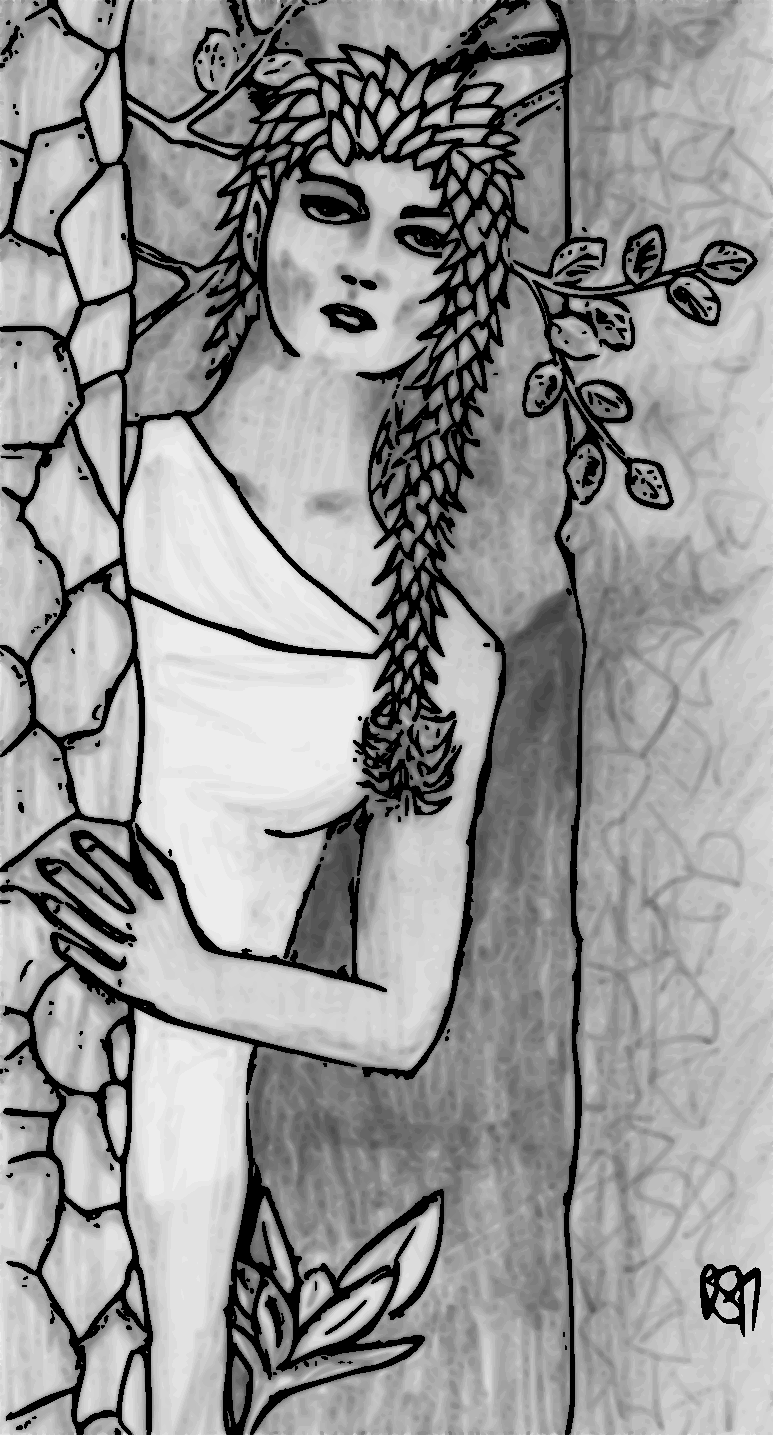
\includegraphics[width=\columnwidth]{southerndryad.pdf}\label{southerndryad}

The creature must be recreated taking into account its new physical abilities and limitations, and the GM must take an active role in the recreation process.  A reincarnated creature retains its knowledge, memories, intelligence, wisdom, and charisma of its old form; however, it gains all physical abilities associated with its new form, including forms of movement and speed, natural armor, natural attacks, special abilities, etc., but it doesn't automatically speak the language or understand the culture of the new form.  The GM may also assign a $-2$ penalty to all actions until the creature becomes familiar with the new form.  The creature's new strength, dexterity, and constitution scores depend on the new form.  If the new form is humanoid, use a method for generating ability scores as determined by the GM to determine 3 new scores and apply racial ability score modifiers found on the charts below.  Typical average ability scores are given on the chart for possible animal forms, and the GM must consult the bestiary to assign other abilities that are typical for the species.  

The following additional guidelines are designed to limit abuse of the spell.  While a reincarnated creature retains the knowledge of any class abilities and other learned skills from its former life, it's highly likely that a change in the creature's form and/or ability scores will make it difficult or even impossible to use those abilities to pursue its previous character class.  The GM will usually rule that all racial restrictions to class, level limits and physical abilities apply.  If the new form allows a character to pursue his original class or one within the same class group (human ranger to hobgoblin fighter or elven mage to gnomish illusionist), he returns to life with half his original levels and hit points.  If the new form forces a character to choose a new class entirely (human mage to lizardman cleric), he loses half his original hit points and begins his new class at 1\textsuperscript{st} level.  If the new form is an animal or other unusual form that does not allow a class, the character loses half his hit points and starts his new life with the lowest HD rating of an adult creature of his kind, rather than a character level.  In any case, the GM should permit a character to earn experience, advance in levels, or otherwise progress as far as his new form will allow, even if an animal form is determined.  For example, a character reincarnated into the body of a badger still has the intellect and knowledge of his former self and thus could be allowed to wear specially crafted armor, use magic items not requiring a comprehensible command word, gain bonus hit points per HD from high constitution and/or combat bonuses from high or exceptional strength, eventually grow to giant size (attaining maximum hit dice for his kind), etc.  

A \textit{wish} cast in conjunction with this spell can fully restore a reincarnated creature to its original form and full class abilities.  If the GM allows, a \textit{limited wish} cast in conjunction with this spell may restore a creature to its original race (but not original form), or it may allow the character to pursue his former class in the body of a creature not normally allowed.

The material components are a small drum and a minimum of a drop of blood or other small part that was attached to the creature's body at the time of death.  The GM may allow certain rare incense, oils and unguents, worth a total of least 1,000 gp, to be used to increase the chances for the body of a specific race or species to be created.

The priests' version of this spell functions in a similar manner to the wizards' spell of the same name with the following differences.  The person may be dead for up to one week per caster level, and the GM may choose to use divine intervention to influence the new form in any manner he feels appropriate.  The caster's holy or unholy symbol serves in place of the small drum, but unlike the drum, it is not lost in the casting of the spell.

\index{Ability Scores!Adjustments for Reincarnation}\index{Age!Adjustments for Reincarnation}\index{Races!and Reincarnation}\index{Thief Abilities!Racial Adjustments!from Reincarnation}The following charts provide much needed information required to create and flesh out the non-standard humanoid characters that often result from the application of this spell.  The GM must refer to the bestiary for any additional information, but remember the reincarnated character only gains the new form's natural abilities.

\noindent
\begin{minipage}{\columnwidth}

\noindent
\captionof{table}{Reincarnate: Wizard's Table}
\begin{tabular}{|p{.15\columnwidth}|p{.3\columnwidth}|p{.1\columnwidth}|p{.1\columnwidth}|p{.1\columnwidth}|}
\hline
\multicolumn{2}{|c|}{ }	& \multicolumn{3}{c|}{Ability Modifiers} \\
1d100	& New Form	& Str	& Dex	& Con \\
\hline\hline
\rowcolor[gray]{0.9}01--05	& Bugbear	& +1	& +0	& +0 \\
06--11	& Dwarf	& +0	& $-1$	& +1 \\
\rowcolor[gray]{0.9}12--18	& Elf	& +0	& +1	& $-1$ \\
19--23	& Gnoll	& +1	& +0	& +0 \\
\rowcolor[gray]{0.9}24--28	& Gnome	& +0	& +0	& +0 \\
29--33	& Goblin	& $-1$	& +0	& +0 \\
\rowcolor[gray]{0.9}34--40	& Half-elf	& +0	& +0	& +0 \\
41--47	& Halfling	& $-1$	& +1	& +0 \\
\rowcolor[gray]{0.9}48--52	& Half-ogre	& +1	& +0	& +1 \\
53--59	& Half-orc	& +1	& +0	& +1 \\
\rowcolor[gray]{0.9}60--65	& Hobgoblin	& +0	& +0	& +0 \\
66--79	& Human	& +0	& +0	& +0 \\
\rowcolor[gray]{0.9}80--85	& Kobold	& $-1$	& +0	& $-1$ \\
86--90	& Lizardman	& +0	& +0	& +0 \\
\rowcolor[gray]{0.9}91--95	& Mongrelman	& \multicolumn{3}{c|}{+1 player's choice} \\
96--00	& Orc	& +0	& $-1$	& +1 \\
\hline
\end{tabular}

\end{minipage}

\noindent
\begin{minipage}{\columnwidth}

\noindent
\captionof{table}{Reincarnate: Priest's Table}
\begin{tabular}{|p{.15\columnwidth}|p{.3\columnwidth}|p{.1\columnwidth}|p{.1\columnwidth}|p{.1\columnwidth}|}
\hline
\multicolumn{2}{|c|}{ }	& \multicolumn{3}{c|}{Ability Modifiers} \\
1d100	& New Form	& Str	& Dex	& Con \\
\hline\hline
\rowcolor[gray]{0.9}01--03	& Badger	& 8	& 17	& 15 \\
04--08	& Bear, black	& 19	& 13	& 15 \\
\rowcolor[gray]{0.9}09--12	& Bear, brown	& 20	& 13	& 19 \\
13--16	& Boar, wild	& 15	& 10	& 17 \\
\rowcolor[gray]{0.9}17--19	& Centaur	& +0	& $-2$	& +1 \\
20--23	& Dryad	& +0	& +1	& $-1$ \\
\rowcolor[gray]{0.9}24--28	& Eagle	& 10	& 15	& 12 \\
29--31	& Elf	& +0	& +1	& $-1$ \\
\rowcolor[gray]{0.9}32--34	& Fox	& 13	& 17	& 15 \\
35--36	& Gnome	& +0	& +0	& +0 \\
\rowcolor[gray]{0.9}37--40	& Hawk	& 6	& 17	& 10 \\
41--44	& Human	& +0	& +0	& +0 \\
\rowcolor[gray]{0.9}45--58	& Lynx	& 16	& 19	& 15 \\
59--61	& Owl	& 4	& 17	& 10 \\
\rowcolor[gray]{0.9}62--64	& Pixie	& $-1$	& +1	& $-1$ \\
65--68	& Raccoon	& 5	& 16	& 12 \\
\rowcolor[gray]{0.9}69--70	& Satyr	& +0	& +1	& +1 \\
71--75	& Stag	& 15	& 20	& 12 \\
\rowcolor[gray]{0.9}76--80	& Wolf	& 13	& 15	& 15 \\
81--85	& Wolverine	& 14	& 15	& 19 \\
\rowcolor[gray]{0.9}86--00	& \multicolumn{4}{c|}{GM Choice or Roll on Wizard's Table} \\
\hline
\end{tabular}

\end{minipage}

\noindent
\begin{minipage}{\columnwidth}

\noindent
\captionof{table}{Humanoid Minimum/Maximum Ability Scores}
\begin{tabular}{|p{.35\columnwidth}|p{.15\columnwidth}|p{.15\columnwidth}|p{.15\columnwidth}|}
\hline
Race	& Str	& Dex	& Con \\
\hline\hline
\rowcolor[gray]{0.9}Bugbear	& 8/19	& 8/17	& 8/18 \\
Centaur	& 11/18	& 3/16	& 11/19 \\
\rowcolor[gray]{0.9}Dryad	& 5/18	& 6/19	& 3/17 \\
Gnoll	& 6/19	& 5/18	& 5/18 \\
\rowcolor[gray]{0.9}Goblin	& 4/15	& 4/17	& 5/16 \\
Half-Ogre	& 14/19	& 3/12	& 14/19 \\
\rowcolor[gray]{0.9}Half-Orc	& 6/19	& 3/17	& 13/19 \\
Hobgoblin	& 6/18	& 6/18	& 5/18 \\
\rowcolor[gray]{0.9}Kobold	& 3/16	& 4/18	& 4/15 \\
Lizardman	& 8/18	& 3/18	& 6/18 \\
\rowcolor[gray]{0.9}Mongrelman	& 6/17	& 6/18	& 8/18 \\
Orc	& 6/18	& 3/17	& 8/19 \\
\rowcolor[gray]{0.9}Pixie	& 3/14	& 8/19	& 7/16 \\
Satyr	& 6/18(75)	& 8/19	& 7/19 \\
\hline
\end{tabular}

\end{minipage}

\end{multicols}

\noindent
\begin{minipage}{\textwidth}

\noindent
\captionof{table}{Humanoid Class Level Limits}
\begin{tabular}{|p{.12\textwidth}|p{.08\textwidth}|p{.08\textwidth}|p{.08\textwidth}|p{.08\textwidth}|p{.41\textwidth}|}
\hline
New Form	& War	& Wiz	& Prs	& Rog	& Multi-Class Options \\
\hline\hline
\rowcolor[gray]{0.9}Bugbear	& 12F	& 0	& 8C	& 9T	& fighter/cleric, fighter/thief, cleric/thief \\
Centaur	& 12F, 10R	& 12M	& 14D	& 12B	& fighter/mage \\
\rowcolor[gray]{0.9}Dryad	& 7F, 8R	& 7M	& 9D	& 12T, 14B	& fighter/mage, ranger/mage, fighter/thief, ranger/thief, mage/thief \\
Gnoll	& 11F	& 0	& 9C	& 11T	& fighter/cleric, fighter/thief \\
\rowcolor[gray]{0.9}Goblin	& 10F	& 0	& 9C	& 12T	& fighter/cleric, fighter/thief, cleric/thief \\
Half-ogre	& 12F	& 0	& 4C	& 0	& fighter/cleric \\
\rowcolor[gray]{0.9}Half-orc	& 10F	& 0	& 4C	& 8T	& fighter/cleric, fighter/thief, cleric/thief \\
Hobgoblin	& 11F	& 0	& 9C	& 12T	& fighter/cleric, fighter/thief \\
\rowcolor[gray]{0.9}Kobold	& 8F	& 0	& 9C	& 12T	& fighter/cleric, fighter/thief, cleric/thief \\
Lizardman	& 12F	& 0	& 7C	& 9T	& fighter/cleric, fighter/thief \\
\rowcolor[gray]{0.9}Mongrelman	& 10F	& 10M	& 10C	& 12T, 8B	& fighter/cleric, cleric/thief, mage/thief, cleric/mage \\
Orc	& 10F	& 0	& 9C	& 11T	& fighter/cleric, fighter/thief, cleric/thief \\
\rowcolor[gray]{0.9}Pixie	& 7F	& 0	& 0	& 12T	& fighter/thief \\
Satyr	& 11F	& 0	& 0	& 11T	& fighter/thief \\
\hline
\end{tabular}
\noindent\begin{tabular}{p{.98\textwidth}}
Key--F=Fighter, R=Ranger, M=Mage, C=Cleric, D=Druid, T=Thief, B= Bard) \\
\end{tabular}\vspace{.5em}

\end{minipage}

\noindent
\begin{minipage}{\textwidth}

\noindent
\captionof{table}{Humanoid Thief Ability Adjustments}
\begin{tabular}{|p{.13\textwidth}|p{.08\textwidth}|p{.08\textwidth}|p{.08\textwidth}|p{.08\textwidth}|p{.08\textwidth}|p{.08\textwidth}|p{.08\textwidth}|p{.08\textwidth}|}
\hline
New Form	& Pick Pockets	& Open Locks	& Find/ Remove	& Move Stealthily	& Hide in Shadows	& Detect Noise	& Climb Walls	& Read Lang. \\
\hline\hline
\rowcolor[gray]{0.9}Bugbear		& $-5$\%	& $-5$\%	& --	& +10\%	& +10\%	& +5\%	& $-5$\%	& $-10$\% \\
Centaur		& --	& --	& --	& --	& --	& --	& NA	& $-5$\% \\
\rowcolor[gray]{0.9}Dryad		& --	& --	& --	& --	& +5\%	& +5\%	& --	& -- \\
Gnoll		& $-5$\%	& $-5$\%	& --	& --	& +5\%	& +5\%	& --	& $-10$\% \\
\rowcolor[gray]{0.9}Goblin		& +5\%	& --	& +10\%	& +5\%	& +5\%	& --	& $-10$\%	& $-10$\% \\
Half-orc	& $-5$\%	& +5\%	& +5\%	& --	& --	& +5\%	& +5\%	& $-10$\% \\
\rowcolor[gray]{0.9}Hobgoblin	& --	& +5\%	& +5\%	& --	& --	& --	& --	& $-10$\% \\
Kobold		& +5\%	& --	& --	& +5\%	& +10\%	& +10\%	& $-15$\%	& $-10$\% \\
\rowcolor[gray]{0.9}Lizardman	& $-5$\%	& $-5$\%	& --	& +5\%	& +5\%	& +5\%	& $-5$\%	& $-5$\% \\
Mongrelman*	& +5\%	& --	& --	& +5\%	& +5\%	& +5\%	& $-5$\%	& $-5$\% \\
\rowcolor[gray]{0.9}Orc			& $-5$\%	& --	& --	& --	& +5\%	& +5\%	& +5\%	& $-10$\% \\
Pixie		& +5\%	& $-10$\%	& --	& +5\%	& +10\%	& +5\%	& --	& -- \\
\rowcolor[gray]{0.9}Satyr		& +5\%	& $-5$\%	& --	& +5\%	& +5\%	& --	& $-10$\%	& $-5$\% \\
\hline
\end{tabular}
\noindent\begin{tabular}{p{.98\textwidth}}
*Mongrelman also gains an additional 5\% bonus to the ability of the player's choice \\
\end{tabular}\vspace{.5em}

\end{minipage}

\noindent
\begin{minipage}{\textwidth}

\noindent
\captionof{table}{Humanoid Height and Weight}
\begin{tabular}{|p{.17\textwidth}|p{.18\textwidth}|p{.17\textwidth}|p{.18\textwidth}|p{.17\textwidth}|}
\hline
New Form	& Base Height	& Modifier	& Base Weight	& Modifier \\
\hline\hline
\rowcolor[gray]{0.9}Bugbear	& 72"/68"	& 1d6	& 210 lbs./180 lbs.	& 6d10 \\
Centaur	& 84"/80"	& 3d12	& 1000 lbs./960 lbs.	& 6d20 \\
\rowcolor[gray]{0.9}Dryad	& --/59"	& 2d10	& --/100 lbs.	& 6d10 \\
Gnoll	& 84"/80"	& 1d12	& 180 lbs./160 lbs.	& 4d10 \\
\rowcolor[gray]{0.9}Goblin	& 43"/41"	& 1d10	& 72 lbs./68 lbs.	& 5d4 \\
Half-ogre	& 84"/78"	& 2d6	& 270 lbs./220 lbs.	& 6d10 \\
\rowcolor[gray]{0.9}Half-orc	& 60"/58"	& 1d12	& 135 lbs./95 lbs.	& 6d10 \\
Hobgoblin	& 72"/68"	& 1d8	& 150 lbs./130 lbs.	& 5d10 \\
\rowcolor[gray]{0.9}Kobold	& 32"/30"	& 3d4	& 52 lbs./48 lbs.	& 5d4 \\
Lizardman	& 60"/60"	& 2d12	& 170 lbs./170 lbs.	& 3d10 \\
\rowcolor[gray]{0.9}Mongrelman	& 60"/59"	& 2d12	& 145 lbs./105 lbs.	& 4d10 \\
Orc	& 58"/56"	& 1d12	& 135 lbs./95 lbs.	& 6d10 \\
\rowcolor[gray]{0.9}Pixie	& 15"/13"	& 1d4	& 25 lbs./22 lbs.	& 1d4 \\
Satyr	& 55"/--	& 1d10	& 110 lbs./--	& 4d10 \\
\hline
\end{tabular}

\end{minipage}

\noindent
\begin{minipage}{\textwidth}

\noindent
\captionof{table}{Humanoid Age}
\begin{tabular}{|p{.12\textwidth}|p{.11\textwidth}|p{.12\textwidth}|p{.12\textwidth}|p{.12\textwidth}|p{.11\textwidth}|p{.12\textwidth}|}
\hline
New Form	& Starting Age	& Variable	& Max Age	& Middle Age*	& Old Age**	& Venerable*** \\
\hline\hline
\rowcolor[gray]{0.9}Bugbear	& 10	& 1d6	& 65+2d10	& 33	& 44	& 65 \\
Centaur	& 18	& 1d4	& 75+2d20	& 37	& 50	& 75 \\
\rowcolor[gray]{0.9}Dryad	& 19	& 2d4	& 171+3d20	& 71	& 121	& 171 \\
Gnoll	& 7	& 1d4	& 33+1d4	& 16	& 22	& 33 \\
\rowcolor[gray]{0.9}Goblin	& 12	& 1d6	& 40+1d20	& 20	& 27	& 40 \\
Half-ogre	& 15	& 1d4	& 90+2d20	& 45	& 60	& 90 \\
\rowcolor[gray]{0.9}Half-orc	& 12	& 1d4	& 60+1d20	& 30	& 40	& 60 \\
Hobgoblin	& 14	& 1d6	& 50+1d20	& 25	& 33	& 50 \\
\rowcolor[gray]{0.9}Kobold	& 12	& 1d4	& 95+2d20	& 48	& 62	& 95 \\
Lizardman	& 15	& 1d4	& 110+2d10	& 55	& 73	& 110 \\
\rowcolor[gray]{0.9}Mongrelman	& 6	& 1d4	& 30+1d10	& 15	& 20	& 30 \\
Orc	& 10	& 1d4	& 35+1d10	& 17	& 23	& 35 \\
\rowcolor[gray]{0.9}Pixie	& 106	& 5d6	& 200+2d100	& 100	& 133	& 200 \\
Satyr	& 20	& 3d4	& 100+1d100	& 50	& 67	& 100 \\
\hline
\end{tabular}
\noindent\begin{tabular}{p{.98\textwidth}}
* $-1$ Str/Con; +1 Int/Wis \\
** $-2$ Str/Dex, $-1$ Con; +1 Wis \\
*** $-1$ Str/Dex/Con; +1 Int/Wis \\
\end{tabular}\vspace{.5em}

\end{minipage}

\begin{multicols}{2}

\vspace{1em}

\noindent
\begin{minipage}{\columnwidth}

\noindent \textbf{Remove Curse (Universal)}

\noindent \textbf{Caster/Level (Sphere):} Priest/3 (All), Wizard/4

\noindent \textbf{Range:} Touch

\noindent \textbf{Duration:} Permanent

\noindent \textbf{Effective Area:} Special

\noindent \textbf{Components:} V and S

\noindent \textbf{Casting Time:} Priest---6, Wizard---4

\noindent \textbf{Saving Throw:} Special

\end{minipage}

\textit{Remove curse} typically (but not always) enables a creature afflicted with an accursed magical item to get rid of the accursed item, but most often the item remains cursed, except in the case of magical cursed scrolls (\textit{remove curse} destroys a targeted cursed scroll).  The spell is also used to counter the effects of magical cursed scrolls, its reverse, \textit{bestow curse}, and similar curses, however, certain special curses may not be countered by this spell or may be countered only by a caster of a certain level or higher.  The spell can also counter lycanthropy, remove insanity caused from contact other plane, and cure the sicken effect of an eye bite spell. 

\noindent
\begin{tabular}{|p{.2\columnwidth}|p{.7\columnwidth}|}
\hline
1d100	& Result \\
\hline\hline
\rowcolor[gray]{0.9}1--50	& Lowers an ability score to 3 (roll 1d6 to determine randomly) \\
51--75	& Inflicts a $-4$ penalty to attack rolls and saves \\
\rowcolor[gray]{0.9}76--00	& Subject is 50\% likely each round to drop any items it is holding and do nothing \\
\hline
\end{tabular}

The reverse, \textit{bestow curse}, places a curse on the subject.  The caster must roll a successful touch attack, and the victim gains a save vs. spell to avoid the effect.  Curses last one turn per caster level.  They cannot be removed by \textit{dispel magic}, but can be removed with a \textit{limited wish}, \textit{remove curse}, or \textit{wish} spell.

The caster may also invent his own curse, but it should be no more powerful than those described above. 

\vspace{1em}

\noindent
\begin{minipage}{\columnwidth}

\noindent \textbf{Remove Fear (Abjuration)}

\noindent \textbf{Caster/Level (Sphere):} Priest/1 (Charm)

\noindent \textbf{Range:} 10 yards

\noindent \textbf{Duration:} Special

\noindent \textbf{Effective Area:} 1 creature per 4 levels

\noindent \textbf{Components:} V and S

\noindent \textbf{Casting Time:} 1

\noindent \textbf{Saving Throw:} Special

\end{minipage}

This spell makes a creature or creatures within range feel more courageous.  The effect provides a +4 bonus to the subject's saving throws against fear attacks for one turn.  If a subject is currently under the effects of a magical fear attack, it is immediately granted a new saving throw with a +4 bonus to overcome the effect.  Casting the reverse on a subject negates the effects, automatically.

The reverse, \textit{cause fear}, causes one creature within range to flee for 1d4 rounds.  The subject is allowed a saving throw, modified by wisdom---mental defense modifier, to avoid the effect.  Casting \textit{remove fear} on a subject automatically negates the effects.

Neither the spell nor its reverse directly affects the undead, but can be used to counter the effects of a fear attack from an undead.

\noindent
\includegraphics[width=3.6in, height=1.25in]{testblock.pdf}

\vspace{1em}

\noindent
\begin{minipage}{\columnwidth}

\noindent \textbf{Remove Paralysis (Abjuration)}

\noindent \textbf{Caster/Level (Sphere):} Priest/3 (Protection)

\noindent \textbf{Range:} 10 yards/level

\noindent \textbf{Duration:} Permanent

\noindent \textbf{Effective Area:} 1-4 creatures in a 20-foot cube

\noindent \textbf{Components:} V and S

\noindent \textbf{Casting Time:} 6

\noindent \textbf{Saving Throw:} Special

\end{minipage}

This spell frees up to 4 creatures, within the spell's range and effective area, from paralyzation effects, including ghoul attacks, or related magical effects, such as \textit{hold} or \textit{slow}.  

If this spell is cast on only one creature, the paralyzation effect is instantly negated.  If this spell is cast on two creatures, they are both allowed a new saving throw against the effect with a +4 bonus.   If three or more creatures are targeted, each gets a new save with a +2 bonus.  For the spell to be effective, there must be no physical or magical barrier blocking the caster from his targeted subjects.

\vspace{1em}

\noindent
\begin{minipage}{\columnwidth}

\noindent \textbf{Repel Insects (Abjuration, Transmutation)}

\noindent \textbf{Caster/Level (Sphere):} Priest/4 (Animal, Protection)

\noindent \textbf{Range:} 0

\noindent \textbf{Duration:} 1 turn/level

\noindent \textbf{Effective Area:} 10-foot radius

\noindent \textbf{Components:} V, S and M

\noindent \textbf{Casting Time:} 1 round

\noindent \textbf{Saving Throw:} None

\end{minipage}

This spell creates an invisible barrier against all kinds of insects.  Normal insects and giant insects with less than $^1$/$_3$ the caster's levels in HD are not able to enter the effective area for the duration of the spell.  Monstrous insects with $^1$/$_3$ or more HD than the caster has levels can enter the effective area if they roll a successful save vs. spell, but they suffer 1d6 points of damage when passing through the barrier.  

This spell has no effect on arachnids, crustaceans, other non-insect vermin, or intelligent insect-like creatures.

The material component is one of the following: crushed marigold flowers, crushed leek, crushed stinging nettle leaves, or a small lump of camphor resin.

\vspace{1em}

\noindent
\begin{minipage}{\columnwidth}

\noindent \textbf{Repulsion (Abjuration)}

\noindent \textbf{Caster/Level:} Wizard/6

\noindent \textbf{Range:} 0

\noindent \textbf{Duration:} 1 round per 2 levels

\noindent \textbf{Effective Area:} 10 feet wide~$\times$~10 feet per level long

\noindent \textbf{Components:} V, S and M

\noindent \textbf{Casting Time:} 6

\noindent \textbf{Saving Throw:} None

\end{minipage}

This spell allows the caster to point in a specific direction and force all creatures in the effective area to move away from the caster.  Each round, the caster can continue to point in the same direction, point in a new direction or perform a different action.  Affected creatures move away at their highest movement value for at least one round, until the caster stops pointing or chooses another direction, even if this causes them to move beyond the effective area.

The material component is a small pair of magnetized bars made of iron attached to two small dog figurines, one made of ivory and one made of ebony.

\vspace{1em}

\noindent
\begin{minipage}{\columnwidth}

\noindent \textbf{Resilient Sphere (Transmutation, Evocation)}

\noindent \textbf{Caster/Level:} Wizard/4

\noindent \textbf{Range:} 20 yards

\noindent \textbf{Duration:} 1 round/level

\noindent \textbf{Effective Area:} 1-foot diameter/level

\noindent \textbf{Components:} V, S and M

\noindent \textbf{Casting Time:} 4

\noindent \textbf{Saving Throw:} Negate

\end{minipage}

This spell allows the caster to trap one creature inside a globe of shimmering force.  The spell fails if the subject is larger than the sphere or makes a successful save.  The sphere imprisons the subject for the duration of the spell, but it can be destroyed by a \textit{rod of cancellation}, \textit{wand of negation}, \textit{disintegrate}, or \textit{dispel magic}, releasing the imprisoned subject unharmed.  Nothing except normal air can pass in or out through the sphere, so that the subject can breathe normally.  The imprisoned subject can move the sphere, or creatures pushing from the outside can move it.

The material components are a matched set of hemispheres, one made of a hard, clear gemstone (diamond is preferred) and the other made of gum arabic.

\vspace{1em}

\noindent
\begin{minipage}{\columnwidth}

\noindent \textbf{Resist Fire/Resist Cold (Transmutation)}

\noindent \textbf{Caster/Level (Sphere):} Priest/2 (Protection)

\noindent \textbf{Range:} Touch

\noindent \textbf{Duration:} 1 round/level

\noindent \textbf{Effective Area:} 1 creature

\noindent \textbf{Components:} V, S and M

\noindent \textbf{Casting Time:} 5

\noindent \textbf{Saving Throw:} None

\end{minipage}

This spell assists a creature to resist the effects of either heat or cold (as determined by the caster at the time if the casting).  The caster may also choose to be the subject.  Depending on the spell effect chosen, the subject becomes immune to either freezing temperatures as low as $-30$$^\circ$F or ordinary heat as high as 130$^\circ$F, including brief contact with ordinary flames (1 round or less).  The subject also gains a +3 bonus to saving throws against more intense heat or cold attacks, whether magical or mundane in nature (red-hot coals, large amounts of burning oil, \textit{flame tongue swords}, \textit{fire storms}, \textit{fireballs}, \textit{meteor swarms}, red dragon's breath, \textit{frost brand swords}, \textit{ice storms}, \textit{wands of frost}, white dragon's breath, etc.).  The subject then suffers only 25\% of the normal damage if the save is successful and only 50\% of the normal damage if the save fails.
 
The material component is a drop of mercury.

\vspace{1em}

\noindent
\begin{minipage}{\columnwidth}

\noindent \textbf{\textit{Restoration} (Necromancy)}

\noindent \textbf{Caster/Level (Sphere):} Priest/7 (Necromantic)

\noindent \textbf{Range:} Touch

\noindent \textbf{Duration:} Permanent

\noindent \textbf{Effective Area:} 1 creature

\noindent \textbf{Components:} V and S

\noindent \textbf{Casting Time:} 3 rounds

\noindent \textbf{Saving Throw:} None

\end{minipage}

This spell restores 1 drained level from a creature provided the level was lost within one day per caster level.  The spell raises the character's experience points to the minimum number required to regain one level.  It also heals feeble mind, confusion and many other insanity effects.  This spell ages both the caster and subject by two years if his venerable age is 150 years or less, four years if his venerable age is between 151 and 250 years, six years if his venerable age is between 251 and 350 years, etc.

The reverse, \textit{energy drain}, drains 1 level from a creature via a successful touch attack, in the same manner as a powerful undead.  The reverse does not cause the caster or the victim to unnaturally age.

\vspace{1em}

\noindent
\begin{minipage}{\columnwidth}

\noindent \textbf{\textit{Resurrection} (Necromancy)}

\noindent \textbf{Caster/Level (Sphere):} Priest/7 (Necromantic)

\noindent \textbf{Range:} Touch

\noindent \textbf{Duration:} Permanent

\noindent \textbf{Effective Area:} 1 creature

\noindent \textbf{Components:} V, S and M

\noindent \textbf{Casting Time:} 1 turn

\noindent \textbf{Saving Throw:} None

\end{minipage}

This spell restores life, limb and full health to any dead creature, including elves and others with spirits, provided they have been dead 10 years per caster level or less.  A complete body is not necessary, as this spell forms a new body from the remains and natural elements at hand, however, if only a small amount of the creature's body remains intact, the GM may wish to assign penalties to the creature's constitution---resurrection chance.  The small part must have been attached to the creature at the time of its death.  Poison, disease, and other afflictions are absent from the new body.  The new body is the same age as the old; so that the spell cannot be used to raise a creature that has died of old age.  A character turned into an undead and then destroyed, as well as some other types of undead, can be resurrected, but constructs, elementals, and creatures from the outer planes can't be resurrected.  A creature to be resurrected must roll his constitution---resurrection chance.  If successful, the creature immediately loses 1 point of constitution permanently, but is restored to life and full hit points.  In addition, the resurrected character retains the ability to cast any spells that he had remaining in his memory at the time of his death.  A character's starting constitution is the maximum number of times he can ever be raised from the dead in his own body.  If he fails his constitution---resurrection chance, only a wish can restore his life to his original body.

Casting this spell ages a caster three years if his venerable age is 150 years or less, six years if his venerable age is between 151 and 250 years, nine years if his venerable age is between 251 and 350 years, etc.  The caster must rest completely for one day per level or HD of the revived creature.  

On a successful touch attack, the reverse, \textit{destruction}, instantly slays a creature and turns it to dust, unless the creature saves vs. death magic with a $-4$ penalty.  A \textit{wish} or divine intervention is required to bring the creature back to life.  If the save is successful, the creature suffers 8d6 points of damage, which may still kill it, but not turn the body to dust.  The reverse does not unnaturally age the caster.

The material components are the caster's holy or unholy symbol and holy or unholy water. 

\vspace{1em}

\noindent
\begin{minipage}{\columnwidth}

\noindent \textbf{Reverse Gravity (Transmutation)}

\noindent \textbf{Caster/Level:} Wizard/7

\noindent \textbf{Range:} 5 yards/level

\noindent \textbf{Duration:} $^1$/$_1$$_0$$_0$ of a second/level

\noindent \textbf{Effective Area:} 30 feet~$\times$~30 feet

\noindent \textbf{Components:} V, S and M

\noindent \textbf{Casting Time:} 7

\noindent \textbf{Saving Throw:} None

\end{minipage}

This spell reverses the flow of gravity with respect to objects and creatures within the spell's range.  The spell causes unattached objects and creatures in the effective area to ``fall" upward, and if they strike a solid object, they suffer damage as if they had fallen normally.  The creatures and objects remain under the spell's effect for the spell's duration, falling up to 1.67 feet per caster level.  When the effects end, gravity returns to normal for the objects and creatures, and they fall back downward, possibly taking falling damage again.  

The material components are a lodestone and iron filings.  
 
\vspace{1em}

\noindent
\begin{minipage}{\columnwidth}

\noindent \textbf{Rope Trick (Transmutation)}

\noindent \textbf{Caster/Level:} Wizard/2

\noindent \textbf{Range:} Touch

\noindent \textbf{Duration:} 2 turns/level

\noindent \textbf{Effective Area:} Special

\noindent \textbf{Components:} V, S and M

\noindent \textbf{Casting Time:} 2

\noindent \textbf{Saving Throw:} None

\end{minipage}

When cast upon a rope between 5 and 30-feet long, this spell allows the rope to attach to an inter-dimensional space, 10' high, 10' long, and 20' wide.  During the casting, one end of the rope rises into the air and fastens itself to this space.  The caster and up to seven other man-sized creatures can climb up the rope and vanish into the space.  

The rope can be brought into the space, but counts as a whole creature.  If not brought into the space, the rope hangs visibly in mid-air.  Creatures cannot see into it, but there is an invisible 3-foot~$\times$~5-foot window centered on the rope that allows creatures inside the space to see out.  A creature weighing over 2 tons or that otherwise makes a successful bend bars check can break the connection between an exposed rope and the space, trapping the occupants inside the space until the spell ends.

No sort of spell effect or other attack can cross into or out of the space, including divinations, unless the effect can cross planes.  Only one creature at a time can climb the rope, during which time it is still in normal space.  When the spell ends the rope drops, the inter-dimensional space collapses and everything inside falls to the ground below.  

The GM may rule that additional spell effects creating and accessing Inter-dimensional Space, such as another \textit{rope trick} or a \textit{deep pockets} spell, etc., simply fail to work while inside the \textit{rope trick}, but that accessing Non-dimensional Space inside of an inter-dimensional space is extremely dangerous (Refer to \textit{bag of holding} and \textit{portable hole}).

The material components are a piece of parchment twisted into a loop and a handful of powdered corn extract.
 
\vspace{1em}

\noindent \textbf{\subsection{S}}

\noindent
\begin{minipage}{\columnwidth}

\noindent \textbf{Sanctuary (Abjuration)}

\noindent \textbf{Caster/Level (Sphere):} Priest/1 (Protection)

\noindent \textbf{Range:} Touch

\noindent \textbf{Duration:} 2 rounds~+~1 round/level

\noindent \textbf{Effective Area:} 1 creature

\noindent \textbf{Components:} V, S and M

\noindent \textbf{Casting Time:} 4

\noindent \textbf{Saving Throw:} None

\end{minipage}

This spell allows the caster to create an invisible safe haven around his person, or another creature designated by touch, as protection against being attacked.  Any enemy who attempts to physically attack or directly target the protected creature with any harmful effects must save vs. spell.  Failure indicates the enemy aborts the current attack, and for the remainder of the spell's duration completely ignores the protected creature and forgets his existence.  Enemies who never attempt to attack the protected creature are not affected, and the effect does not protect the creature from spells such as \textit{fireball} or \textit{ice storm} that cover an effective area.  If the protected creature attempts to inflict damage or otherwise directly harm an enemy, the spell ends, however, he may perform any other actions, such as cure wounds, cast divinations, chant, etc.  

The material components are a small silver mirror and the caster's holy or unholy symbol.

\vspace{1em}

\noindent
\begin{minipage}{\columnwidth}

\noindent \textbf{Scare (Enchantment)}

\noindent \textbf{Caster/Level:} Wizard/2

\noindent \textbf{Range:} 30 yards~+~10 yards/level

\noindent \textbf{Duration:} 1d4 rounds~+~1 round/level

\noindent \textbf{Effective Area:} 1 creature/ 3 levels, within a 15-foot radius

\noindent \textbf{Components:} V, S and M

\noindent \textbf{Casting Time:} 2

\noindent \textbf{Saving Throw:} Special

\end{minipage}

This spell besets one or more creatures, within range, inside the effective area, and with less than 6 HD or levels, with a fit of trembling fear.  The spell has no affect on undead or creatures from the outer planes, but otherwise only elves, half-elves, and priests are granted a saving throw, modified by wisdom---mental defense modifier, to avoid the effect.  If lightly encumbered or more, drops any item(s) it may be holding.  The creature is also demoralized, but if forced to fight, suffers a $-1$ penalty to attacks, damage (each die of damage for an unarmed creature), and saving throws.  A frightened creature suffers a $-2$ charisma---reaction modifier for the spell's duration, allowing more favorable reaction results for the caster, especially if attempting to capture, interrogate or recruit the creature.

The material component is a bone fragment from an undead skeleton, zombie, ghoul, ghast, or mummy.

\vspace{1em}

\noindent
\begin{minipage}{\columnwidth}

\noindent \textbf{Screen (Greater Divination, Illusion)}

\noindent \textbf{Caster/Level:} Wizard/8

\noindent \textbf{Range:} 0

\noindent \textbf{Duration:} 1 hour/level

\noindent \textbf{Effective Area:} 30-foot cube/level

\noindent \textbf{Components:} V and S

\noindent \textbf{Casting Time:} 1 turn

\noindent \textbf{Saving Throw:} Special

\end{minipage}

This spell creates a powerful illusory effect that changes what can or cannot be seen, felt, smelt and heard within the effective area, by either scrying or direct observation.  The effect is declared in simple terms, it cannot be programmed with more than one type of activity, or set of conditions, and the effect cannot be changed once created, for the duration of the spell.  So that an illusion may be created of the caster playing a game with pen, paper and strange dice with a group of friends while he is actually casting a spell or not even in the vicinity at all, but the illusion must play the same game for the whole duration of the spell.  An empty field with chirping birds could be made to appear as an active military camp, or the reverse.  An army passing through the effective area can be made totally invisible, or be made to appear more or less numerous, and/or better or more poorly equipped than they actually are.  Many other uses are possible.

Those attempting to scry the effective area automatically believe the illusion, but direct observers may be allowed a saving throw, modified by wisdom---mental defense modifier and appropriate believability modifiers, if they have some reason to disbelieve the effect, (Refer to Illusions).  Even if the viewer enters the effective area, the illusion is not automatically ended nor does he necessarily gain a saving throw, as long as any unseen creature(s) inside the effective area avoid those under the effect of the illusion.  If a direct observer has a vantage point that allows him to see the edge(s) of the effective area and therefore can see troops appear, disappear, seem to change armor, etc., this is reason to disbelieve the illusion.  The effect can be ended by a successful \textit{dispel magic}.

\vspace{1em}

\noindent
\begin{minipage}{\columnwidth}

\noindent \textbf{Secret Page (Transmutation)}

\noindent \textbf{Caster/Level:} Wizard/3

\noindent \textbf{Range:} Touch

\noindent \textbf{Duration:} Until dispelled

\noindent \textbf{Effective Area:} 1 page, up to 2-foot square

\noindent \textbf{Components:} V, S and M

\noindent \textbf{Casting Time:} 1 turn

\noindent \textbf{Saving Throw:} None

\end{minipage}

This spell allows the caster to alter the contents of a page to appear as a completely different page.  Maps can look like recipes; recipes look like spells, spells like book keeping records, etc.  If magic is detected for, the secret page radiates a dim magical aura.  In addition, \textit{confuse languages}, \textit{explosive runes} or \textit{sepia snake sigil} can be cast on a secret page.

The caster can speak a command word (chosen at the time of casting), which suspends this spell's effect and reveals the page's true contents.  After perusing the page, the caster can restore the effect at will.  The secret page is otherwise permanent, until destroyed or the caster ends it by speaking the command word twice in succession.

Comprehend languages used alone has no effect and true seeing only reveals the presence of hidden material, but if cast together, they can reveal the true content, without ending the spell or destroying the page.  

The effect can be ended by a successful \textit{dispel magic}, but a failed attempt destroys the page.  A successful \textit{erase} spell will also destroy the original writing without revealing it.

The material components are the essence of a will o'wisp or boggart, combined with powdered herring scales.

\vspace{1em}

\noindent
\begin{minipage}{\columnwidth}

\noindent \textbf{Seeming (Illusion)}

\noindent \textbf{Caster/Level:} Wizard/5

\noindent \textbf{Range:} 10-foot radius

\noindent \textbf{Duration:} 12 hours

\noindent \textbf{Effective Area:} 1 person per 2 levels

\noindent \textbf{Components:} V and S

\noindent \textbf{Casting Time:} 5

\noindent \textbf{Saving Throw:} Negate

\end{minipage}

This spell functions as the \textit{change self} spell except that it allows the caster to change the appearance of one or more persons within range (and he may choose to include himself).  Targeted creatures that do not wish to have their appearance changed are granted a saving throw to avoid the effect.  All affected creatures must resemble the same race of humanoid.  If a subject dies before the spell duration expires, the spell effect ends prematurely for that subject only, and it returns to its normal appearance.  

Note: As with \textit{change self}, this is an illusory effect and creatures that interact with a subject may be allowed a saving throw, modified by wisdom---mental defense and appropriate believability modifiers, if they have some reason to disbelieve the effect.  The GM may determine that a will not be affected if the appearance change would violate the height differential stated for the spell effect (for instance, a 3' halfling could not be made to look like a bugbear), however, the GM may allow the effect to work within the height strictures, so that the halfling appears as an unusually short or very young bugbear, which may prompt a disbelief check.
 
\vspace{1em}

\noindent
\begin{minipage}{\columnwidth}

\noindent \textbf{Sending (Evocation)}

\noindent \textbf{Caster/Level:} Wizard/5

\noindent \textbf{Range:} Unlimited

\noindent \textbf{Duration:} Special

\noindent \textbf{Effective Area:} 1 creature

\noindent \textbf{Components:} V, S and M

\noindent \textbf{Casting Time:} 1 turn

\noindent \textbf{Saving Throw:} None

\end{minipage}

This spell allows the caster to send a mental message to a single creature whose name and appearance are well known to him. The recipient will recognize the caster, if it knows him.  The message must be 25 words or less, and even creatures with animal intelligence can understand it.  The creature can choose to answer the message immediately in 25 words or less, or choose to ignore the message.  Those with animal intelligence cannot answer in words, but may respond empathically.  

If the requested creature is not physically on the same plane as the caster, there's a base 5\% chance the spell fails.  The GM may determine that circumstances on the receiving plane and each intervening plane may increase this chance of failure.  

The material components are two tiny metal cylinders, each open on one end, and connected to each other by a small piece of finely twisted copper wire.

\vspace{1em}

\noindent
\begin{minipage}{\columnwidth}

\noindent \textbf{Sepia Snake Sigil (Conjuration)}

\noindent \textbf{Caster/Level:} Wizard/3

\noindent \textbf{Range:} 5 yards

\noindent \textbf{Duration:} Special

\noindent \textbf{Effective Area:} 1 sigil

\noindent \textbf{Components:} V, S and M

\noindent \textbf{Casting Time:} 3

\noindent \textbf{Saving Throw:} None

\end{minipage}

This spell allows the caster to scribe a small symbol within the text of any written body of work.  When the text containing the symbol is read, a dark brownish grey snake springs from the page and immediately attacks the nearest living creature (usually the reader) within range, but the snake will not attack the caster.  The snake strikes as a monster with HD equal to the caster's level at the time the spell was cast.  If the attack is successful, the snake transforms into a shimmering amber force field around the victim, completely immobilizing it for 1d4~+~1 days per caster level at the time of the casting, until released by the caster, or until a successful \textit{dispel magic} is cast.  No form of attack or magical effect can move the force field or damage the victim.  While inside the force field, the victim is in a state of timeless suspended animation (See \textit{Temporal Stasis}).  If the attack fails, the sepia snake dissipates with a loud noise, a flash of brown light and a puff of dun-colored smoke, 10 feet in diameter and lasting for one round. 

The small symbol cannot be detected by normal visual inspection, while a \textit{detect magic} spell only reveals that the entire text is magical.  A successful \textit{dispel magic} can remove the symbol without destroying the page, but \textit{erase} destroys the sigil along with the entire page of text.  The spell can be cast in combination with other spells that change, garble or hide text.

The spell components are a snake's scale, a pinch of mushroom spores, and powdered amber of 100 gp value.

\vspace{1em}

\noindent
\begin{minipage}{\columnwidth}

\noindent \textbf{Sequester (Illusion, Abjuration)}

\noindent \textbf{Caster/Level:} Wizard/7

\noindent \textbf{Range:} Touch

\noindent \textbf{Duration:} 1 week~+~1 day/level

\noindent \textbf{Effective Area:} 2-foot cube/level

\noindent \textbf{Components:} V, S and M

\noindent \textbf{Casting Time:} 7

\noindent \textbf{Saving Throw:} Special

\end{minipage}

This spell renders everything in the effective area invisible to any form of vision, including scrying attempts, and undetectable by locate and detect spells.  The spell can thus hide a secret door, treasure vault, statue, etc., but the affected object is still tangible and can be found through touch and revealed by using certain magical items (like a \textit{robe of eyes} or \textit{gem of seeing}).  

The spell can be cast upon living creatures within the effective area (including the undead, but not constructs, elementals or creatures from the outer planes).  An unwilling creature gains a saving throw to avoid the effect.  If the save fails, the creature not only becomes invisible and undetectable but also falls into a coma and is placed in a state of suspended animation (See \textit{Temporal Stasis}), until the duration expires or a successful \textit{dispel magic} is cast.    

The material components are the eyelash of a basilisk, gum arabic, and a dram ($^1$/$_8$ of an ounce) of whitewash.

\vspace{1em}

\noindent
\begin{minipage}{\columnwidth}

\noindent \textbf{Shades (Illusion)}

\noindent \textbf{Caster/Level:} Wizard/6

\noindent \textbf{Range:} 30 yards

\noindent \textbf{Duration:} 1 round/level

\noindent \textbf{Effective Area:} 20-foot cube

\noindent \textbf{Components:} V and S

\noindent \textbf{Casting Time:} 6

\noindent \textbf{Saving Throw:} Special

\end{minipage}

This spell functions as \textit{shadow monsters}, except that the quasi-real creatures each have 60\% of the normal hit points.  If disbelieved, they deal 60\% damage and have AC 6.  

\vspace{1em}

\noindent
\begin{minipage}{\columnwidth}

\noindent \textbf{Shadow Door (Illusion)}

\noindent \textbf{Caster/Level:} Wizard/5

\noindent \textbf{Range:} 10 yards

\noindent \textbf{Duration:} 1 round/level

\noindent \textbf{Effective Area:} Special

\noindent \textbf{Components:} S

\noindent \textbf{Casting Time:} 2

\noindent \textbf{Saving Throw:} None

\end{minipage}

This spell creates an illusory door that the caster appears to step through, but the caster actually becomes invisible (Refer to \textit{Invisibility}) for the spell's duration, and can flee to one side or the other.  The illusory door also remains for the spell's duration, and creatures that open it believe they see and can enter an empty 10-foot~$\times$~10-foot room on the other side.  Casting true seeing or similar magical means can spot the caster.  Creatures with high HD have the normal chance to notice the invisible caster, but they must actively attempt to use the ability. 

\vspace{1em}

\noindent
\begin{minipage}{\columnwidth}

\noindent \textbf{Shadow Magic (Illusion)}

\noindent \textbf{Caster/Level:} Wizard/5

\noindent \textbf{Range:} 50 yards~+~10 yards/level

\noindent \textbf{Duration:} Special

\noindent \textbf{Effective Area:} Special

\noindent \textbf{Components:} V and S

\noindent \textbf{Casting Time:} 5

\noindent \textbf{Saving Throw:} Special

\end{minipage}

This spell allows the caster to draw energy from the Demiplane of Shadow to cast quasi-real arcane spells from the school of evocation of not more than 3\textsuperscript{rd} level (\textit{magic missile}, \textit{fireball}, \textit{lightning bolt}, etc.).  Creatures struck by a quasi-real effect automatically gain a saving throw to disbelieve it, which if successful, reduces damage to 20\% of normal.  If the quasi-real spell allows a save, it is rolled normally.

\vspace{1em}

\noindent
\begin{minipage}{\columnwidth}

\noindent \textbf{Shadow Monsters (Illusion)}

\noindent \textbf{Caster/Level:} Wizard/4

\noindent \textbf{Range:} 30 yards

\noindent \textbf{Duration:} 1 round/level

\noindent \textbf{Effective Area:} 20-foot cube

\noindent \textbf{Components:} V and S

\noindent \textbf{Casting Time:} 4

\noindent \textbf{Saving Throw:} Special

\end{minipage}

This spell allows the caster to pull strands of material from the Demiplane of Shadow out of thin air to create up to 1 HD per caster level worth of quasi-real monsters.  All creatures created by a single casting must be of the same type.  Each monster retains its normal attack values, armor class, saving throws, and special abilities, but only 20\% of the hit points it would normally have (round up .4 or more).  If this hit point reduction results in a monster with less than 0.4 hit points, the monster fails to materialize.  Creatures viewing the quasi-real monsters are allowed a chance to disbelieve with a $-2$ penalty (Refer to Illusions).  Those who fail the saving throw suffer normal damage from all attacks and behave as if special attacks that do not inflict damage, such as gaze effects, petrification, level drain, etc., were real, until a successful \textit{dispel magic} is cast on the illusory monsters, or a heal is cast on the illusory effects.  

Creatures that successfully disbelieve quasi-real monsters see them as transparent images superimposed on shadowy forms.  To them, the quasi-real monsters have AC 10, inflict only 20\% of the normal damage from attacks (discard damage less than .4), and they aren't affected by the quasi-real monster's special attacks.

\vspace{1em}

\noindent
\begin{minipage}{\columnwidth}

\noindent \textbf{Shadow Walk (Illusion, Enchantment)}

\noindent \textbf{Caster/Level:} Wizard/7

\noindent \textbf{Range:} Touch

\noindent \textbf{Duration:} 6 turns/level

\noindent \textbf{Effective Area:} Special

\noindent \textbf{Components:} V and S

\noindent \textbf{Casting Time:} 1

\noindent \textbf{Saving Throw:} None

\end{minipage}

This spell can only be cast in an area of heavy shadows, but then allows the caster to transport his own person, and up to 1 other creature per caster level he is touching, to the border between of the Prime Material Plane and the Demiplane of Shadow.  Unwilling creatures that are touched are allowed a save to avoid the effect.  While in this border region, the caster moves at a rate of 7 miles per turn with respect to the Prime Material Plane and can choose the exact location where he will return.  However, due to the blurring of reality between the Demiplane of Shadow and the Prime Material Plane, he can't make out details of the terrain or areas he passes over during transit, so that the spell is virtually useless for scouting or spying.  

Shadow walk can also be used to travel to other planes that border on the Demiplane of Shadow, but this usage requires traveling across the Demiplane of Shadow to arrive at a border with another plane of reality.  The transit across the Demiplane of Shadow requires 1d4 hours, requiring at least 1 random encounter check.

Creatures brought to this region by the caster may choose to follow the caster, or go their own way.  If they go their own way or are otherwise separated from the caster, they have a 50\% chance to either become lost on the Demiplane of Shadow or find a way back to a random location within one mile from where the spell was cast on the Prime Material Plane. 

\vspace{1em}

\noindent
\begin{minipage}{\columnwidth}

\noindent \textbf{Shape Change (Transmutation)}

\noindent \textbf{Caster/Level:} Wizard/9

\noindent \textbf{Range:} 0

\noindent \textbf{Duration:} 1 turn/level

\noindent \textbf{Effective Area:} The caster

\noindent \textbf{Components:} V, S and M

\noindent \textbf{Casting Time:} 9

\noindent \textbf{Saving Throw:} None

\end{minipage}

This spell allows the caster to assume the form of any living creature below the rank of demigod that he is familiar with (including gaseous form or incorporeal creatures, normal plant-life and the undead, but excluding constructs and elementals).  Size is not a factor, but the assumed form cannot have more than the caster's level in Hit Dice (to a maximum of 25 HD).  The caster retains his own current hit point total, intelligence, wisdom and charisma, and does not gain the creature's innate magical abilities or magic resistance, but does gain all of its strength, dexterity, constitution, movement value(s), physical abilities, and vulnerabilities.  

Changing shape requires only a second, and no constitution---system shock roll is necessary, allowing the caster to freely change his shape once per round while performing other actions, such as during combat.  If the caster is killed, the spell ends, but the caster does not revert to his original form, and this may prevent the caster from being brought back to life by magic that requires his original body.

The material component is a jade circlet worth at least 5,000 gp, which shatters when the spell ends.  The circlet remains upon the caster's head for the duration of the spell, and if it's destroyed (via a called shot, or by failing a save versus an attack that would destroy it), the spell ends prematurely.

\vspace{1em}

\noindent
\begin{minipage}{\columnwidth}

\noindent \textbf{Shatter (Transmutation)}

\noindent \textbf{Caster/Level:} Wizard/2

\noindent \textbf{Range:} 30 yards~+~10 yards/level

\noindent \textbf{Duration:} Instantaneous

\noindent \textbf{Effective Area:} 3-foot radius

\noindent \textbf{Components:} V, S and M

\noindent \textbf{Casting Time:} 2

\noindent \textbf{Saving Throw:} Negate

\end{minipage}

This spell produces a sonic (sound based) attack that affects mundane objects made of crystal, glass, ceramic, or porcelain (including vials, bottles, flasks, jugs, windows, mirrors, etc.).  

This spell has two effects.  The specific effect is chosen when the spell is cast.

\textbf{Blast the Area:} All appropriate objects weighing 1 pound per caster level or less, within range and caught in the effective area, must save vs. crushing blow or break into a dozen or more small pieces.  

\textbf{Target One:} This effect is targeted against a single appropriate object, within range, of up to 10 pounds per caster level.  It must save vs. crushing blow or break into hundreds of small pieces.  This effect can also be cast upon a single crystalline creature.  The creature suffers 1d6 points of damage per caster level, to a maximum of 6d6.  A successful saving throw vs. spell reduces this damage to half.

The material component is a chip of mica.

\vspace{1em}

\noindent
\begin{minipage}{\columnwidth}

\noindent \textbf{Shield (Evocation)}

\noindent \textbf{Caster/Level:} Wizard/1

\noindent \textbf{Range:} 0

\noindent \textbf{Duration:} 5 rounds/level

\noindent \textbf{Effective Area:} Special

\noindent \textbf{Components:} V and S

\noindent \textbf{Casting Time:} 1

\noindent \textbf{Saving Throw:} None

\end{minipage}

This spell allows the caster to protect the front of his person with a magical barrier during combat.  The invisible field completely negates the effects of \textit{magic missiles} against the front of his person.  It also provides a +1 bonus to saving throws, AC 2 versus hurled weapons (axe, dart, javelin, spear, etc.), AC 3 versus propelled missiles (arrow, bolt, manticore spike, sling bullets and stones, etc.), and AC 4 versus any other attacks or effects that come from in front of the caster.  

\vspace{1em}

\noindent
\begin{minipage}{\columnwidth}

\noindent \textbf{Shillelagh (Transmutation)}

\noindent \textbf{Caster/Level (Sphere):} Priest/1 (Combat, Plant)

\noindent \textbf{Range:} Touch

\noindent \textbf{Duration:} 4 rounds~+~1 round/level

\noindent \textbf{Effective Area:} 1 oak club

\noindent \textbf{Components:} V, S and M

\noindent \textbf{Casting Time:} 2

\noindent \textbf{Saving Throw:} None

\end{minipage}

This spell allows the caster to enchant his mundane wooden club or staff to temporarily become in all ways magical.  As long as the caster wields the weapon during the spell's duration, it gains a +1 bonus to attack rolls and inflicts 2d4 points of damage to man-sized and smaller creatures or 1d4~+~1 points of damage to large creatures.

The material components are the leaf of a shamrock and the caster's holy or unholy symbol.  The weapon is unharmed by the effect.

\vspace{1em}

\noindent
\begin{minipage}{\columnwidth}

\noindent \textbf{Shocking Grasp (Transmutation)}

\noindent \textbf{Caster/Level:} Wizard/1

\noindent \textbf{Range:} Touch

\noindent \textbf{Duration:} 1 round/level

\noindent \textbf{Effective Area:} 1 creature

\noindent \textbf{Components:} V and S

\noindent \textbf{Casting Time:} 1

\noindent \textbf{Saving Throw:} None

\end{minipage}

This spell allows the caster to deliver a powerful electrical shock to an opponent with a successful touch attack.  The GM may allow up to a +3 attack bonus when used against those made of metal, wearing metal armor, or carrying a lot of metal items.  The spell remains in effect for its duration or until discharged.  A successful attack deals 1d8~+~1 points of damage per caster level.  Touching the caster does not discharge the electricity.

\vspace{1em}

\noindent
\begin{minipage}{\columnwidth}

\noindent \textbf{Shout (Evocation)}

\noindent \textbf{Caster/Level:} Wizard/4

\noindent \textbf{Range:} 0

\noindent \textbf{Duration:} Instantaneous

\noindent \textbf{Effective Area:} 10-foot~$\times$~30-foot cone

\noindent \textbf{Components:} V and M

\noindent \textbf{Casting Time:} 1

\noindent \textbf{Saving Throw:} Special

\end{minipage}

This spell allows the caster to produce a high volume sonic attack, deafening creatures in the effective area for 2d6 rounds and inflicting 2d6 points of damage.  A successful save allows a creature to avoid the deafness and halves the damage.  The effect shatters exposed brittle or crystalline objects within the effective area.  Those objects in a creature's possession gain a save to avoid the effect.  The effect is blocked by silence, 15' radius.  The spell can only be used once per day; each additional use forces the caster to save vs. spell or become permanently deafened.

The material components are a small cone made from the horn of a bull or a ram, and a drop each of honey and citric acid.

\vspace{1em}

\noindent
\begin{minipage}{\columnwidth}

\noindent \textbf{Silence, 15' Radius (Transmutation)}

\noindent \textbf{Caster/Level (Sphere):} Priest/2 (Guardian)

\noindent \textbf{Range:} 120 yards

\noindent \textbf{Duration:} 2 rounds/level

\noindent \textbf{Effective Area:} 15-foot radius

\noindent \textbf{Components:} V and S

\noindent \textbf{Casting Time:} 5

\noindent \textbf{Saving Throw:} None

\end{minipage}

This spell creates a zone of complete silence in the effective area.  No sound can enter, leave or occur within the effective area, preventing conversation and spell casting that requires verbal components, but also completely protecting those inside from any sonic-based attacks (including harpy song, \textit{shout} spell, \textit{horn of blasting}, etc.).  The effective area can either be stationary, or it cast on a mobile object or creature.  An unwilling creature, or an item possessed by an unwilling creature, is allowed a saving throw.  If successful, the center of the effective area becomes a stationary point approximately one foot behind that creature.  

\vspace{1em}

\noindent
\begin{minipage}{\columnwidth}

\noindent \textbf{Simulacrum (Illusion)}

\noindent \textbf{Caster/Level:} Wizard/7

\noindent \textbf{Range:} Special

\noindent \textbf{Duration:} Permanent

\noindent \textbf{Effective Area:} 1 creature

\noindent \textbf{Components:} V, S and M

\noindent \textbf{Casting Time:} 12 hours

\noindent \textbf{Saving Throw:} None

\end{minipage}

This spell allows the caster to create a quasi-real, exact physical duplicate of any specific creature with HD or levels equal to or less than twice his caster level.  While his creation has the same physical abilities, countenance and general appearance as the original, it is a zombie-like, mindless being that follows the caster's simplest verbal commands.  At this stage, the \textit{simulacrum} is considered a non-intelligent, non-aligned construct.  Its level or HD (for attacks, saves and all other non-learned abilities) is only 20--50\% ((1d4~+~1)~$\times$~10\%) of that of the original creature, and it has a maximum number of hit points between 51 and 60\% (50~+~1d10\%) of the total hit points of the original creature.  Once the \textit{simulacrum} has been created, these two scores will never change, however, the caster may choose to enhance his \textit{simulacrum} in other ways.  If killed, a \textit{simulacrum} (whether enhanced or not) melts and evaporates instantly into water vapor, regardless of the ambient temperature, but a damaged \textit{simulacrum} can be repaired via a complicated alchemical process.  This process requires a fully stocked laboratory, 100 gp worth of ruby dust (or other material the GM feels appropriate) per hit point repaired, and 12-hours~+~1 hour per hit point repaired above 12.  \textit{Detect magic}, \textit{true seeing}, or similar reveals the \textit{simulacrum} for what it is, regardless of enhancements.

The material components are a life-sized body made from ice or snow, a pinch of powdered ruby, and a small piece (feather, scale, lock of hair, fang, tooth, beak, claw, talon or fingernail, etc.) from the creature that is to be duplicated.  The latter is set inside the icy body, usually in the place of the heart, during the casting of the spell.

\textbf{Stage 1 Enhancement:} To enhance the creation, a reincarnate spell is initially used to infuse it with a spirit (or possibly a soul).  The GM may choose to determine the original nature of the life force by rolling d100 and consulting the wizard's (or if desired, priest's) reincarnation table.  The creation is then less zombie-like, gaining intelligence, wisdom, and charisma scores equal to one-third of the original creature's scores (generating scores between 1 and 6).  The duplicate can now speak (and possibly read and write) one language chosen by the caster from those that the original creature knows.  At this stage of the enhancement process, the \textit{simulacrum} is considered a living creature, and feels a self-preservation instinct that will allow it to refuse obviously suicidal commands.  It will also begin to radiate an aura of alignment.  Exactly which alignment is up to the GM, but there are 3 sources to consider, the alignment of the caster, the alignment of the creature being duplicated, and the alignment of the life force that inhabits the body.  While being directly controlled by the caster by either verbal or written commands, the creature tends to radiate the alignment of the caster.  If left alone or undirected for more than 24 hours, the alignment begins to drift towards that of the original creature (75\% chance) or that of the life force (25\% chance).  

\textbf{Stage 2 Enhancement:} A \textit{limited wish} can now be employed to grant the creature learned class abilities of the original (at the previously determined level or HD), and between 40 and 65\% (35~+~5d6\%) of the original's intelligence, wisdom and charisma scores.  This also provides the \textit{simulacrum} with partial knowledge, limited memories, and general personality traits of the original creature.  The GM must then determine personality quirks that are different from the original, incomplete or lost areas of knowledge and memories that the duplicate does not gain.  While making these determinations, the GM may take into consideration the influence of the caster's alignment and personality, the influence of the infused life force, as well as the actions (if any) that the \textit{simulacrum} has been commanded to perform before being enhanced to this stage.  Once determined, the creature cannot gain levels of experience or learn new abilities.  Since the \textit{simulacrum} has now acquired so much of the original creature's mental attributes, the caster's alignment may come into conflict with the original creature's alignment, but the life force's alignment is no longer a factor.  If the caster commands the duplicate to perform an action that is completely at odds with the original creature's alignment (for example, the caster commands a paladin's \textit{simulacrum}, which has been enhanced by both \textit{reincarnate} and \textit{limited wish}, to rampage through a peaceful hamlet, killing innocent peasants and burning their huts to the ground), the \textit{simulacrum} is allowed a saving throw, modified by its wisdom---mental defense modifier, to refuse to follow the command.  The GM may assign an additional penalty up to $-4$ or a bonus up to +4 to the save, depending upon the severity of the alignment conflict, rewards or punishments involved, and other factors. 

\vspace{1em}

\noindent
\begin{minipage}{\columnwidth}

\noindent \textbf{Sink (Enchantment, Transmutation)}

\noindent \textbf{Caster/Level:} Wizard/8

\noindent \textbf{Range:} 10 yards/level

\noindent \textbf{Duration:} Special

\noindent \textbf{Effective Area:} 1 creature or object, 1 cubic foot/level maximum

\noindent \textbf{Components:} V and S

\noindent \textbf{Casting Time:} 8

\noindent \textbf{Saving Throw:} Special

\end{minipage}

This spell attempts to bury a creature or object, within range and up to the effective area in size, by causing the ground below its feet to become temporarily less dense.  

The caster must cast the spell without interruption for at least the remainder of the round.  At the end of the round, the subject becomes rooted to the ground for 4 turns.  Mundane objects get no saving throw, but a creature is granted one save vs. spell, and magical items (including items with any kind of enchantment cast upon them or magical origins) are allowed one save vs. disintegration, to avoid the effect.  If this save is failed and the subject becomes stuck, the caster can continue casting the spell throughout the next round, so that the subject begins to sink into the ground.  Before the group that wins initiative performs its actions, the subject sinks $^1$/$_4$ of its height.  After the first group performs its actions, the subject sinks $^1$/$_2$ of its height, after the second group performs its actions, the subject sinks $^3$/$_4$ of its height, and by the end of the round, the subject is completely buried.
If a subject becomes completely buried, it continues to sink until it becomes entombed in a state of timeless suspended animation (See \textit{Temporal Stasis}), with its highest point at a depth equal to its height.  If \textit{detect magic} is cast over an area where a subject is entombed, a faint magical aura is revealed, regardless of how deep it is buried, however, if it is within the detection spell's range, the schools of alteration and enchantment may also be revealed.

If the ground above and around an affected creature or object can be excavated, the spell ends.  An entombed creature revives from its suspended animation and can climb out, or if an object, it can be hauled out.  \textit{Dig}, \textit{transmute rock to mud}, and \textit{freedom} (Refer to \textit{Imprisonment}) do not harm a partially buried or entombed creature or sunken object and can often be useful in retrieving it.

\vspace{1em}

\noindent
\begin{minipage}{\columnwidth}

\noindent \textbf{Sleep (Enchantment)}

\noindent \textbf{Caster/Level:} Wizard/1

\noindent \textbf{Range:} 30 yards

\noindent \textbf{Duration:} 5 rounds/level

\noindent \textbf{Effective Area:} 30-foot diameter circle

\noindent \textbf{Components:} V, S and M

\noindent \textbf{Casting Time:} 1

\noindent \textbf{Saving Throw:} None

\end{minipage}

This spell causes one or more creatures (excluding undead and other very specific creatures), in range and within the effective area, to fall into a coma-like state.  The spell affects up to 2d4 HD of creatures with less than 4~+~3 HD each.  Unless the caster targets a specific single creature of appropriate HD, the creature(s) with the lowest hit dice are affected first, and partial effects are discarded.  The creatures are not awakened by loud noises and will remain asleep until the spell duration expires, until they are shaken for an entire round, or until they take damage from any source (assuming the damage doesn't kill them first).  

The material component can be any one of the following: a pinch of fine sand, a small handful of rose petals, or a live cricket.

\noindent
\includegraphics[width=3.6in, height=1.25in]{testblock.pdf}

\vspace{1em}

\noindent
\begin{minipage}{\columnwidth}

\noindent \textbf{Slow (Transmutation)}

\noindent \textbf{Caster/Level:} Wizard/3

\noindent \textbf{Range:} 90 yards~+~10 yards/level

\noindent \textbf{Duration:} 3 rounds~+~1 round/level

\noindent \textbf{Effective Area:} 40-foot cube

\noindent \textbf{Components:} V, S and M

\noindent \textbf{Casting Time:} 3

\noindent \textbf{Saving Throw:} Negate

\end{minipage}

This spell attempts to reduce the movement value and number of attacks per round by half of up to one creature per caster level, in range and within the effective area.  Affected creatures also suffer a +4 penalty to AC, an attack penalty of $-4$, and lose all dexterity bonuses, for the spell's duration.  

The creatures are each granted a saving throw to avoid the effect, but with a $-4$ penalty.  Creatures near the center of the effective area make their saves first, then the next farther out, until the maximum numbers of creatures are affected, or no more creatures are in the effective area.  

This spell cancels the effects of a haste spell or its equivalent, negating both effects, but it does not cancel other magical types of speed, nor can it stack with another slow spell.

The material component is one drop of molasses.  

\vspace{1em}

\noindent
\begin{minipage}{\columnwidth}

\noindent \textbf{Slow Poison (Necromancy)}

\noindent \textbf{Caster/Level (Sphere):} Priest/2 (Healing)

\noindent \textbf{Range:} Touch

\noindent \textbf{Duration:} 1 hour/level

\noindent \textbf{Effective Area:} 1 creature

\noindent \textbf{Components:} V, S and M

\noindent \textbf{Casting Time:} 1

\noindent \textbf{Saving Throw:} None

\end{minipage}

If cast before a poison takes full effect, this spell slows the poison's onset time within an envenomed creature.  The poison is not neutralized but is prevented from farther harming the creature for the spell's duration.  

The material components are the caster's holy or unholy symbol and a bud of crushed garlic, either spread upon an envenomed wound or eaten by an envenomed creature to slow ingested poisons.

\vspace{1em}

\noindent
\begin{minipage}{\columnwidth}

\noindent \textbf{Snake Charm (Enchantment)}

\noindent \textbf{Caster/Level (Sphere):} Priest/2 (Animal)

\noindent \textbf{Range:} 30 yards

\noindent \textbf{Duration:} Special

\noindent \textbf{Effective Area:} 30-foot cube

\noindent \textbf{Components:} V and S

\noindent \textbf{Casting Time:} 5

\noindent \textbf{Saving Throw:} None

\end{minipage}

This spell creates a pattern that hypnotizes a number of serpentine, reptilian creatures, in range and within the effective area.  The snakes' total maximum hit points cannot exceed the caster's maximum total hit points.   The affected snakes will stay in place, only able to sway back and forth in a semi-erect posture for the duration of the spell.  This spell can be effective against any variety of snakes, including giant snakes, snake-like monsters, and intelligent snake-like beings (naga, couatl, etc.), as long as the hit point total is not exceeded.  There is no save, but magic resistance still applies.

The spell's duration is dependent upon the attitude of the snakes when the spell is cast.  If the snakes are completely inactive or asleep, the duration is 1d4~+~2 turns.  If they are active and alert (but not hostile or agitated), the duration is 1d3 turns.  If they are hostile when the spell is cast, the duration is 1d4~+~4 rounds. 

If the GM so desires, this spell can be faith-specific and be modified for use against other creatures significant to particular deities, pantheons, etc.

\vspace{1em}

\noindent
\begin{minipage}{\columnwidth}

\noindent \textbf{Snare (Enchantment)}

\noindent \textbf{Caster/Level (Sphere):} Priest/3 (Plant)

\noindent \textbf{Range:} Touch

\noindent \textbf{Duration:} Until triggered

\noindent \textbf{Effective Area:} 2-foot diameter~+~2 inches/level

\noindent \textbf{Components:} V, S and M

\noindent \textbf{Casting Time:} 3 rounds

\noindent \textbf{Saving Throw:} None

\end{minipage}

This spell makes a magic snare trap. The snare can be made from any supple vine, a thong, or a rope.  As the spell is cast, the cordlike object blends with its surroundings, making it 90\% undetectable to normal, non-magical methods. One end of the snare is tied in a loop that contracts around one or more of the limbs of any creature stepping inside of it.  The neck can sometimes be considered a limb (particularly with snakes and worms, but giraffe also springs to mind).  If a strong and supple tree is nearby, the snare can be fastened to it.  The spell causes the tree to bend and then straighten when the loop is triggered, inflicting 1d6 points of damage to the creature trapped and lifting it off the ground by the trapped limb(s).  The trapped creature may suffocate if the neck is caught.  If no such tree is available (or the caster simply chooses not to use one), the cordlike object magically wraps and entangles around the creature, dealing no damage.  If used underwater, the snare additionally wraps itself around an anchoring point to avoid drifting in the currents.  

The snare is magically strong.  To escape during the first hour of being trapped, a creature requires a strength score of 23 and a full round.  Every hour that passes after the first reduces the strength score required by 1 point, until 6 hours after being captured have passed, when a strength score of only 18 is required.  The snare has AC 7 and 5 hit points.  It can be cut or broken by any magical weapon, or by any mundane edged weapon whose wielder has at least a +2 bonus to attack, either from magical enhancement and/or strength modifier.  If a creature successfully escapes from the snare, the loop breaks and the spell ends.  Otherwise, 12 hours after trapping a victim, the snare loses its enchantment and loosens automatically to release the creature.

The material components are the skin from a snake and sinew from a strong animal, which are weaved into the cordlike object, as well as the caster's holy or unholy symbol.

\vspace{1em}

\noindent
\begin{minipage}{\columnwidth}

\noindent \textbf{Solid Fog (Transmutation)}

\noindent \textbf{Caster/Level:} Wizard/4

\noindent \textbf{Range:} 30 yards

\noindent \textbf{Duration:} 2d4 rounds~+~1 round/level

\noindent \textbf{Effective Area:} 20 feet~$\times$~10 feet~$\times$~10 feet/level of caster

\noindent \textbf{Components:} V, S and M

\noindent \textbf{Casting Time:} 4

\noindent \textbf{Saving Throw:} None

\end{minipage}

This spell functions like \textit{fog cloud}, but in addition to obscuring sight, the \textit{solid fog} is so thick that any creature attempting to move through it progresses at a speed of 1 foot per round, regardless of its normal speed, and suffers a $-2$ penalty on all melee attack and melee damage rolls.  The vapors prevent effective ranged weapon attacks (except for magic rays and the like).  A creature or object that falls into solid fog is slowed, so that each 10 feet of vapor that it passes through reduces falling damage by 1d6.

The fog can be made to fill the effective area or can be made as small as a 10-foot by 10-foot cube.  A gust of wind spell does not affect it, but a very strong wind (greater than 30 mph) will dissipate the vapors in one round.  A \textit{fireball}, \textit{flame strike}, or \textit{wall of fire} will burn it away in one round.

\textit{Solid fog} can be made permanent with a \textit{permanency spell}.  A permanent \textit{solid fog} dispersed by wind reforms in 10 minutes. 

The material components are a pinch of dried, powdered peas combined with powdered animal hoof.

\vspace{1em}

\noindent
\begin{minipage}{\columnwidth}

\noindent \textbf{Speak With Animals (Transmutation)}

\noindent \textbf{Caster/Level (Sphere):} Priest/2 (Animal, Divination)

\noindent \textbf{Range:} 0

\noindent \textbf{Duration:} 2 rounds/level

\noindent \textbf{Effective Area:} 1 animal within 30 feet

\noindent \textbf{Components:} V and S

\noindent \textbf{Casting Time:} 5

\noindent \textbf{Saving Throw:} None

\end{minipage}

This spell allows the caster two-way communication with any natural, mundane animals, including giant animals, whether warm or cold-blooded, so long as they have an intelligence score of 1 or higher.  This includes creatures such as apes, bears, cats, dogs, elephants, etc.

The caster can ask questions and receive answers, but the animal is not necessarily friendly or cooperative.  The GM may wish to roll an encounter reaction check, modified by the caster's charisma---reaction modifier.  If the animal has a friendly reaction or the caster is a druid or other nature-related priest, it may do some additional favor or service for the priest (as determined by the DM).  Those animals with an indifferent reaction may answer or they may simply make absurd comments, while animals with cautious or more hostile reactions will be terse and intentionally evasive. 

\vspace{1em}

\noindent
\begin{minipage}{\columnwidth}

\noindent \textbf{Speak With Dead (Necromancy)}

\noindent \textbf{Caster/Level (Sphere):} Priest/3 (Divination)

\noindent \textbf{Range:} Touch

\noindent \textbf{Duration:} Special

\noindent \textbf{Effective Area:} 1 creature

\noindent \textbf{Components:} V, S and M

\noindent \textbf{Casting Time:} 1 turn

\noindent \textbf{Saving Throw:} Special

\end{minipage}

This spell allows the caster to ask a dead creature a number of questions and possibly receive answers.  The caster receives the answers in his mind.  A dead creature's knowledge is limited to what it knew in life, including its spoken languages, so the caster must be able to speak a language that the creature knew in life.  An unwilling dead creature with either a different alignment than the caster, or higher HD at the time of death than the caster level, is granted a saving throw to resist the spell.  A successful save means the creature refuses to answer and the spell ends.  Each individual dead creature can be spoken to no more than once per week.  

The caster level determines the length of time the creature can have been dead, the number of questions that can be asked, and how much time is allowed to ask them, according to the table below:  

\noindent
\begin{tabular}{|p{.2\columnwidth}|p{.2\columnwidth}|p{.2\columnwidth}|p{.2\columnwidth}|}
\hline
Caster Level	& Max. Time Dead	& Question Time	& Number of Questions \\
\hline\hline
\rowcolor[gray]{.9}1--7	& 1 week	& 1 round	& 2 \\
7--8	& 1 month	& 3 rounds	& 3 \\
\rowcolor[gray]{.9}9--12	& 1 year	& 1 turn	& 4 \\
13--15	& 10 years	& 2 turns	& 5 \\
\rowcolor[gray]{.9}16--20	& 100 years	& 3 turns	& 6 \\
21+	& 1,000 years	& 1 hour	& 7 \\
\hline
\end{tabular}

Dead creatures can answer truthfully, however, they rather tend to take questions from the living in a very literal sense, and their answers are often brief, evasive and cryptic.

The material components are the caster's holy or unholy symbol, burning incense, and some part of the dead creature's bodily remains.  The creature's remains are not destroyed by this spell.

\vspace{1em}

\noindent
\begin{minipage}{\columnwidth}

\noindent \textbf{Speak With Monsters (Transmutation)}

\noindent \textbf{Caster/Level (Sphere):} Priest/6 (All)

\noindent \textbf{Range:} 30 yards

\noindent \textbf{Duration:} 2 rounds/level

\noindent \textbf{Effective Area:} The caster

\noindent \textbf{Components:} V and S

\noindent \textbf{Casting Time:} 9

\noindent \textbf{Saving Throw:} None

\end{minipage}

This spell functions as \textit{speak with animals}, except that it allows the caster two-way communication with any living creature (with an intelligence of 1 or higher), regardless of what form that communication takes (including via pheromones, tactile, empathic, etc.).  The caster can speak to different types of creatures with the same casting, but only one type of creature at a time, per round, until the spell duration expires.  

\vspace{1em}

\noindent
\begin{minipage}{\columnwidth}

\noindent \textbf{Speak With Plants (Transmutation)}

\noindent \textbf{Caster/Level (Sphere):} Priest/4 (Plant)

\noindent \textbf{Range:} 0

\noindent \textbf{Duration:} 1 round/level

\noindent \textbf{Effective Area:} 30-foot radius

\noindent \textbf{Components:} V, S and M

\noindent \textbf{Casting Time:} 1 turn

\noindent \textbf{Saving Throw:} None

\end{minipage}

This spell functions as \textit{speak with animals}, except that it allows the caster a very basic two-way communication with every plant within the effective area, including both normal, mundane plants and plant creatures (including vegetables, fungi, molds, and plantlike monsters).  

Treat a plant creature or plantlike monster, with an intelligence score of at least 1, in all ways as if it were an animal for purposes of determining encounter reaction.  Normal plants, however, will always have a friendly reaction to the caster, though their sense of surroundings is limited, and they aren't able to provide (or recognize) detailed descriptions of creatures or answer questions about events outside their immediate vicinity.  Normal plants cannot uproot themselves and walk around, but they can be made to move and stretch in a manner similar to the entangle spell.  They can be made to part to allow passage, entangle the caster's opponents (as the spell), release a creature caught in the effects of an entangle spell, or perform similar actions.  

The material components are a burning pinch of dung and a drop of water.

\vspace{1em}

\noindent
\begin{minipage}{\columnwidth}

\noindent \textbf{Spectral Force (Illusion)}

\noindent \textbf{Caster/Level:} Wizard/3

\noindent \textbf{Range:} 60 yards~+~1 yard/level

\noindent \textbf{Duration:} Special 

\noindent \textbf{Effective Area:} 40-foot cube~+~10-foot cube/level

\noindent \textbf{Components:} V and S

\noindent \textbf{Casting Time:} 3

\noindent \textbf{Saving Throw:} Special

\end{minipage}

This spell functions as \textit{improved phantasmal force}, with better auditory elements and adding olfactory and thermal elements to the illusion.  The spell lasts for three rounds after the caster stops concentration.

\vspace{1em}

\noindent
\begin{minipage}{\columnwidth}

\noindent \textbf{Spectral Hand (Necromancy)}

\noindent \textbf{Caster/Level:} Wizard/2

\noindent \textbf{Range:} 30 yards~+~5 yards/level

\noindent \textbf{Duration:} 2 rounds/level

\noindent \textbf{Effective Area:} 1 opponent/round

\noindent \textbf{Components:} V and S

\noindent \textbf{Casting Time:} 2

\noindent \textbf{Saving Throw:} None

\end{minipage}

This spell allows the caster to create a glowing, wraithlike hand, imbued with a part of his life force.  The hand materializes anywhere within the spell's range and can move as the caster desires, anywhere within the spell's range.  The hand can deliver the caster's touch attack spells, with a +2 bonus, from spells of 4\textsuperscript{th} level or lower that are cast while the spell is in effect.  It can also gain flank or rear attack bonuses, if the caster is in the proper position.  The hand can attack once per round for the spell's duration, or the caster can dismiss the hand at any time prior to the end of the duration.  If the hand is not attacking, it hovers near the caster.  

The hand is incorporeal and thus cannot be harmed by normal weapons and ignores most magical effects, but magical weapons can harm it.  The hand has an AC $-2$.  Damaging the hand ends the spell and inflicts 1d4 points of damage to the caster.  A successful \textit{dispel magic} ends the spell but does not damage the caster.
 
\vspace{1em}

\noindent
\begin{minipage}{\columnwidth}

\noindent \textbf{Spell Immunity---Arcane (Abjuration)}

\noindent \textbf{Caster/Level:} Wizard/8

\noindent \textbf{Range:} Touch

\noindent \textbf{Duration:} 1 turn/level

\noindent \textbf{Effective Area:} 1 creature/4 caster levels

\noindent \textbf{Components:} V, S and M

\noindent \textbf{Casting Time:} 1 round/recipient

\noindent \textbf{Saving Throw:} None

\end{minipage}

This spell allows the caster to grant the subjects a saving throw bonus against wizard and priest spells that grant a normal saving throw, including similar effects from a creature's special abilities and those from magical items.  The caster may choose to be one of the recipients, however, the spell's duration is divided amongst multiple recipients.  If a 16-turn duration is indicated and 4 creatures are affected, the duration is reduced to 4 turns.  Five recipients would reduce the duration to 3 turns and 2 rounds, three recipients would result in duration of 5 turns and 3 rounds, etc.  The amount of the saving throw bonus is a function of the type of magic and the spell level being resisted, according to the following table:

\noindent
\begin{tabular}{|p{.3\columnwidth}|p{.3\columnwidth}|p{.25\columnwidth}|}
\hline
Spell Level	& Wizard Spell	& Priest Spell \\
\hline\hline
\rowcolor[gray]{.9}1\textsuperscript{st}--3\textsuperscript{rd}	& +9	& +7 \\
4\textsuperscript{th}--6\textsuperscript{th}	& +7	& +5 \\
\rowcolor[gray]{.9}7\textsuperscript{th}--8\textsuperscript{th}	& +5	& +3 \\
\hline
\end{tabular}

The material component is at least 500 gp worth of crushed diamond, which is sprinkled over the recipients.  Each recipient must also carry an intact diamond of any value on his person that is not destroyed by the spell.

\vspace{1em}

\noindent
\begin{minipage}{\columnwidth}

\noindent \textbf{Spell Immunity---Divine (Abjuration)}

\noindent \textbf{Caster/Level (Sphere):} Priest/4 (Protection)

\noindent \textbf{Range:} Touch

\noindent \textbf{Duration:} 1 turn/level

\noindent \textbf{Effective Area:} 1 creature

\noindent \textbf{Components:} V, S and M

\noindent \textbf{Casting Time:} 1 round

\noindent \textbf{Saving Throw:} None

\end{minipage}

This spell allows the caster to grant his own person, or a creature that he touches, immunity to any single, specific spell effect named by the caster, whether from a spell, a creature's special ability or a magical item.  It can offer no protection against breath weapons or any type of gaze attacks.  The caster must have personally experienced the named spell effect at least once previously.  The spell cannot affect a creature that is already under the protection of a potion, protection spell, ring, or other magical item.  

The material component(s) is the same (if any) as that of the named spell to be protected against.

\vspace{1em}

\noindent
\begin{minipage}{\columnwidth}

\noindent \textbf{Spell Turning (Abjuration)}

\noindent \textbf{Caster/Level:} Wizard/7

\noindent \textbf{Range:} 0

\noindent \textbf{Duration:} Up to 3 rounds/level

\noindent \textbf{Effective Area:} The caster

\noindent \textbf{Components:} V, S and M

\noindent \textbf{Casting Time:} 7

\noindent \textbf{Saving Throw:} None

\end{minipage}

This spell alters the three physical dimensions to provide the caster with protection from any spell effect that directly targets his person.  Spell effects targeting him are deflected back upon its caster.  This includes spells cast from scrolls and special abilities that mimic spells, but does not protect against effective area spell effects that are not centered or targeted directly on the caster, spell effects that require a touch attack, or spell effects duplicated by magical items.  This spell effect cannot discern between beneficial and harmful spells and attempts to turn all applicable effects. 

The GM secretly determines the exact number of spell levels between seven and ten (1d4~+~6) that can be turned before the spell duration ends.  If the protected caster is targeted by a spell of higher level than the amount of spell turning levels he has remaining, that spell is only partially deflected, and the spell turning effect ends.  For spells that cause damage, both casters take a fraction of the damage.  Divide the amount of the remaining spell turning levels by the spell level of the incoming spell to determine what fraction of the effect is deflected.  The protected caster takes the rest of the damage as his spell turning effect ends.  A partially deflected hold or paralysis spell acts as a slow spell on whichever caster is successfully affected by at least 50\%.  The GM may adjudicate the results of other partially deflected, non-damage causing spells, on a case-by-case basis, however in most instances, each caster can be given a proportional chance to be struck by the full effect.  Saving throws and magic resistance apply as per normal.

If both casters are protected by \textit{spell turning} effects, a magical resonance field is created.  The following table determines the results:

\noindent
\begin{tabular}{|p{.2\columnwidth}|p{.7\columnwidth}|}
\hline
1d100	& Magical Resonance Field Effect \\
\hline\hline
\rowcolor[gray]{.9}01--70	& The spell effect ends with possibly noisy or colorful, but not harmful effects \\
71--80	& The spell effect strikes both casters equally, at full effect* \\
\rowcolor[gray]{.9}81--97	& Both caster's spell turning effects are negated for 1d4 rounds \\
98--00	& An extra-dimensional rift opens, sending both to a random inner plane** \\
\hline
\multicolumn{2}{l}{*Saving throw allowed, as applicable} \\
\multicolumn{2}{l}{**No save or magic resistance allowed} \\
\end{tabular}\vspace{.5em}

The material component is a small silver mirror.

\vspace{1em}

\noindent
\begin{minipage}{\columnwidth}

\noindent \textbf{Spider Climb (Transmutation)}

\noindent \textbf{Caster/Level:} Wizard/1

\noindent \textbf{Range:} Touch

\noindent \textbf{Duration:} 3 rounds~+~1 round/level

\noindent \textbf{Effective Area:} 1 creature

\noindent \textbf{Components:} V, S and M

\noindent \textbf{Casting Time:} 1

\noindent \textbf{Saving Throw:} Negate

\end{minipage}

This spell enables the recipient (which can be the caster or another creature touched) with the ability to climb and travel on vertical surfaces or even hang upside down from ceilings as well as a spider does.  However, slippery surfaces (icy, oily, greased, etc.) negate the effect.  The caster must score a successful touch attack against an unwilling recipient, and the victim is given a saving throw to avoid the effect.  The recipient must have bare hands and feet to climb in this manner, but when doing so never needs to roll a climb walls or similar check for success and has a maximum movement value of 6 (or 3 if lightly encumbered or more).  It cannot, however, run while climbing.  Objects weighing less than 1 lb. stick to the recipient's hands and feet for the spell's duration making spell casting requiring material components practically impossible.  The recipient retains its dexterity---AC modifier (if any) while climbing, and opponents get no special bonus to their attacks against it.  The recipient may be forcibly pulled from a wall or ceiling (or an object may be pulled off of their hands or feet) by a creature with a strength score of 12 or higher.  If the recipient wishes to resist being pulled off a wall or ceiling, it is granted a save versus paralyzation.  The caster can end the spell's effects prior to the end of the spell's duration by speaking a command word.

The material components are a drop of bitumen and a live spider, both of which must be eaten by the subject.

\noindent
\includegraphics[width=3.6in, height=2.75in]{testblock.pdf}

\vspace{1em}

\noindent
\begin{minipage}{\columnwidth}

\noindent \textbf{Spike Growth (Transmutation, Enchantment)}

\noindent \textbf{Caster/Level (Sphere):} Priest/3 (Plant)

\noindent \textbf{Range:} 60 yards

\noindent \textbf{Duration:} 3d4 turns~+~1 turn/level

\noindent \textbf{Effective Area:} 10-foot square/level

\noindent \textbf{Components:} V, S and M

\noindent \textbf{Casting Time:} 6

\noindent \textbf{Saving Throw:} None

\end{minipage}

This spell creates a magical trap.  Typically, spike growth can be cast in any outdoor setting except open water, ice, heavy snow, sandy desert, or bare stone.  Any ground-covering vegetation in the spell's effective area becomes very hard and sharply pointed (as if covered in caltrops) without changing its appearance.  In areas of bare earth, roots and rootlets act in the same way.  Any creature moving on foot into or through the spell's effective area takes 2d4 points of piercing damage for each 10 feet of movement through the spiked area. 

Any creature that takes damage from the spiky trap must also save versus spell or suffer injuries to its feet and legs that slow its movement value by one-third (minimum of 1).  This movement penalty lasts for 24 hours, or until the injured creature receives a heal spell or enough lesser curative spells to restore twice as many hit points as was lost by traversing the trap. 

This magical trap cannot be found or removed by normal means, requiring \textit{true seeing}, a \textit{detect traps} spell, or similar effects.  Even upon entering the effective area and suffering damage, a victim is unable to determine the extent of the trap without magical aid.
 
The material components for this spell are the caster's holy or unholy symbol and either seven sharp thorns or small, sharpened twigs.

\vspace{1em}

\noindent
\begin{minipage}{\columnwidth}

\noindent \textbf{Spike Stones (Transmutation, Enchantment)}

\noindent \textbf{Caster/Level (Sphere):} Priest/5 (Elemental (Earth))

\noindent \textbf{Range:} 30 yards

\noindent \textbf{Duration:} 3d4 turns~+~1 turn/level

\noindent \textbf{Effective Area:} 10-foot square/level, 1 spike/square foot

\noindent \textbf{Components:} V, S and M

\noindent \textbf{Casting Time:} 6

\noindent \textbf{Saving Throw:} None

\end{minipage}

This spell creates a magical trap.  Rocky ground, stone floors, and similar surfaces in the effective area shape themselves into long, sharp points that blend into the background.  This effect impedes progress through an area and may inflict damage.  Any creature moving on foot into or through the spell's effective area moves at half speed, and suffers an attack from the trap each round as if the caster were attacking.  A successful attack roll inflicts 1d4 points of damage.  The attacks begin as soon as the victim enters the trap and continue each round spent in the effective area.  Those who charge or run through the effective area suffer two attacks per round.  Although a victim notices being slowed, the full effects may not be noticed until an attack is successful.  Anyone who carefully observes the effective area (either before or after entering it) is given a 25\% chance to notice the spikes, however, this magical trap cannot be removed by normal means.  

Any creature that takes damage from the spiky trap must also save versus spell or suffer injuries to its feet and legs that slow its movement value by one-half (minimum of 1).  This movement penalty lasts for 24 hours, or until the injured creature receives a heal spell or enough lesser curative spells to restore twice as many hit points as was lost by traversing the trap. 

This spell is most effective when cast to augment a pit trap.  Falling into an augmented pit trap inflicts 6 attacks upon the victim for every 10' fallen, with a +2 bonus to each attack, and every 10 feet fallen provides a cumulative +2 bonus to each damage roll.  Normal falling damage is suffered at the end of the fall, as well.

The material components are four tiny stalactites.

\vspace{1em}

\noindent
\begin{minipage}{\columnwidth}

\noindent \textbf{Spiritual Hammer (Evocation)}

\noindent \textbf{Caster/Level (Sphere):} Priest/2 (Combat)

\noindent \textbf{Range:} 10 yards/level

\noindent \textbf{Duration:} 3 rounds~+~1 round/level

\noindent \textbf{Effective Area:} Special

\noindent \textbf{Components:} V, S and M

\noindent \textbf{Casting Time:} 5

\noindent \textbf{Saving Throw:} None

\end{minipage}

This spell allows the caster to transform his normal war hammer into a magical, ranged weapon, keeping the same basic shape and size but infused with divine energy.  The caster can concentrate on the magical weapon and cause it to attack any visible opponent within range that he chooses.  The weapon attacks as if wielded by the caster, except that no strength or dexterity modifiers are applied to attack or damage rolls.  The weapon attacks creatures based on the direction that the caster is facing, which may allow rear attacks on an opponent that has its back to the caster.  He may choose a different opponent each round as long as it is still in range and visible to the caster.  The weapon inflicts the same damage as a normal war hammer, however, gains a +1 magical enchantment to attack and damage rolls between caster level 1 and 6, +2 between caster level 7 and 12, up to a maximum of +3 at 13th level and above.

The spell ends prior to its normal duration if the caster stops concentrating on it for any reason.  A successful \textit{dispel magic} spell (whether targeted or using an effective area) against either the caster or the weapon will also end the spell before the duration expires.  Magic resistance is checked the first time it is encountered.  If the magic resistance check is successful, the spell ends, otherwise magic resistance is not checked again unless a stronger magic resistance is encountered.

The material component is the normal war hammer, which the caster throws at his first chosen opponent within the spell's range while casting the spell.  The hammer changes into the magical weapon while in mid-air.

\vspace{1em}

\noindent
\begin{minipage}{\columnwidth}

\noindent \textbf{Spook (Illusion)}

\noindent \textbf{Caster/Level:} Wizard/1

\noindent \textbf{Range:} 30 feet

\noindent \textbf{Duration:} Special

\noindent \textbf{Effective Area:} 1 creature

\noindent \textbf{Components:} V and S

\noindent \textbf{Casting Time:} 1

\noindent \textbf{Saving Throw:} Negate

\end{minipage}

This spell allows the caster to appear as someone or something extremely terrifying to a creature within range.  The spell does not affect the undead, and the creature must have an intelligence score of 2 or more.  

The caster must advance menacingly toward the creature during the casting, whereupon the creature is allowed a saving throw versus spell to avoid the effect, modified by wisdom---mental defense modifier and a $-1$ penalty per 2 caster levels (maximum of $-6$ at caster level 12).  A natural roll of 20 always succeeds regardless of penalties, but if the save fails, the victim clutches its items tightly and flees from the caster at its maximum movement value.  An unseen menace formed in the victim's mind then begins to pursue the victim.  The victim gains a new save each round to end the pursuit, modified by wisdom---mental defense modifier, but without the additional penalties, otherwise the duration is permanent, until the save is made or a successful \textit{dispel magic} is cast. 

\vspace{1em}

\noindent
\begin{minipage}{\columnwidth}

\noindent \textbf{Star Shine (Evocation, Illusion)}

\noindent \textbf{Caster/Level (Sphere):} Priest/3 (Sun)

\noindent \textbf{Range:} 10 yards/level

\noindent \textbf{Duration:} 1 turn/level

\noindent \textbf{Effective Area:} 10-foot square/level

\noindent \textbf{Components:} V, S and M

\noindent \textbf{Casting Time:} 6

\noindent \textbf{Saving Throw:} None

\end{minipage}

This spell lights up the effective area with starlight, providing vision equivalent to that on a bright, moonlit night.  The soft light creates shadows, but does not affect infravision.  The effect is partially an illusion, which tricks creatures into believing the area above the effective area (regardless of its true height) is a clear night sky filled with stars.  A successful save to disbelieve only reveals that the stars are not real and the light must not be coming from a magical source.  The spell does not function underwater.

The material components are several holly berries and stalks from the belladonna lily.

\vspace{1em}

\noindent
\begin{minipage}{\columnwidth}

\noindent \textbf{Statue (Transmutation)}

\noindent \textbf{Caster/Level:} Wizard/7

\noindent \textbf{Range:} Touch

\noindent \textbf{Duration:} 1 hour/level

\noindent \textbf{Effective Area:} 1 creature

\noindent \textbf{Components:} V, S and M

\noindent \textbf{Casting Time:} 7

\noindent \textbf{Saving Throw:} Special

\end{minipage}

This spell allows the caster to transform a subject (either himself or a creature touched), along with any garments and equipment worn or carried, into solid stone as hard as granite.  The subject is unable to move in this state.  The initial transformation requires one full round after the spell is cast.  During the transformation there's an 18\% chance, minus the subject's constitution score, that the creature dies.

The subject can return to its normal state, act, and then return instantly to the statue form, as desired, as long as the spell duration is in effect.  Returning to his stone form doesn't require another check to survive.

In statue form, the subject appears to be made completely of stone, yet radiates faint magic if \textit{detect magic} is cast, and it retains its current hit points.  The subject can see, hear, and smell normally, but it does not need to eat or breathe.  Feeling is limited to those sensations that can affect the granite-hard substance of the individual's body. Chipping is equal to a mere scratch, but breaking off one of the statue's arms constitutes serious damage. 

The material component is lime, sand, and a drop of water stirred by an iron bar, such as a nail or spike.

\vspace{1em}

\noindent
\begin{minipage}{\columnwidth}

\noindent \textbf{\textit{Sticks to Snakes} (Transmutation)}

\noindent \textbf{Caster/Level (Sphere):} Priest/4 (Plant)

\noindent \textbf{Range:} 30 yards

\noindent \textbf{Duration:} 2 rounds/level

\noindent \textbf{Effective Area:} 1d4 sticks~+~1 stick/level in a 10-foot cube

\noindent \textbf{Components:} V, S and M

\noindent \textbf{Casting Time:} 7

\noindent \textbf{Saving Throw:} None

\end{minipage}

This spell transforms a number of sticks within the effective area, no smaller than a torch and no larger than a staff, into snakes under the caster's command.  A stick in the possession of a creature can avoid the effect if the creature rolls a successful save vs. polymorph.  Magical items, staves, wands, spears, etc., cannot be transformed by this spell.  If the caster desires at the time of casting, he is given a 5\% chance per caster level to create poisonous snakes.  The snakes generally conform to the following standard abilities, but the GM may determine that these apply only when a staff, spear or similar is used, and reduce these scores when smaller sticks are used.
 
\noindent
\begin{tabular}{|p{.25\columnwidth}|p{.3\columnwidth}|p{.3\columnwidth}|}
\hline
	& Constrictor	& Poisonous \\
\hline\hline
\rowcolor[gray]{.9}Armor Class	& 6	& 6 \\
Movement	& 9	& 15 \\
\rowcolor[gray]{.9}Hit Dice	& 3~+~2	& 2~+~1 \\
THACO	& 17	& 19 \\
\rowcolor[gray]{.9}Attacks	& 2---Bite (1)~+~Constrict (1d3)	& 1---Bite (1)~+~Poison* \\
\hline
\end{tabular}
\noindent\begin{tabular}{p{.95\columnwidth}}
*The poison provides a +2 to the victim's save and has an onset time of 2-5 rounds.  The victim dies unless the save is successful. \\
\end{tabular}\vspace{.5em}

The reverse, \textit{snakes to sticks}, transforms normal-sized, non-magical snakes within the effective area into sticks for the spell's duration. It can also reverse (or partially reverse) the effect of a \textit{sticks to snakes} spell, and vice versa, according to the caster level.

The material components for the spell and its reverse are the correct number of sticks (or live snakes) of the correct size, a small piece of bark and several snake scales.  

If the GM so desires, this spell can be faith-specific and be modified for use with other creatures significant to particular deities, pantheons, etc.

\vspace{1em}

\noindent
\begin{minipage}{\columnwidth}

\noindent \textbf{Stinking Cloud (Evocation)}

\noindent \textbf{Caster/Level:} Wizard/2

\noindent \textbf{Range:} 30 yards

\noindent \textbf{Duration:} 1 round/level

\noindent \textbf{Effective Area:} 20-foot cube

\noindent \textbf{Components:} V, S and M

\noindent \textbf{Casting Time:} 2

\noindent \textbf{Saving Throw:} Special

\end{minipage}

This spell fills the effective area with a billowing mass of nauseous vapors for the spell's duration.  The edge of the cloud nearest the caster can be as far away from the caster as the spell's range.  Any creature within the effective area must roll a successful save vs. poison or immediately become nauseous and unable to perform any action other than move while inside the cloud and for 1d4~+~1 rounds after leaving it.  Those who make the save successfully avoid the nausea if they leave the cloud that round but must roll a new save vs. poison each round if they remain in the cloud.  The poison can be slowed or neutralized by the appropriate spells or abilities.  A breeze between 8 and 18 mph halves the spell's duration, and the cloud is dispersed in one round by stronger winds.

The material component is one rotten egg or several leaves of the skunk cabbage.

\vspace{1em}

\noindent
\begin{minipage}{\columnwidth}

\noindent \textbf{Stone Shape (Transmutation)}

\noindent \textbf{Caster/Level (Sphere):} Priest/3 (Elemental (Earth)), Wizard/5

\noindent \textbf{Range:} Touch

\noindent \textbf{Duration:} Permanent

\noindent \textbf{Effective Area:} Priest---9 cubic feet~+~1 cubic foot/level, Wizard---1 cubic foot/level

\noindent \textbf{Components:} V, S and M

\noindent \textbf{Casting Time:} 1 round

\noindent \textbf{Saving Throw:} None

\end{minipage}

This spell allows the caster to form an existing piece of stone into any shape of the same volume that suits his purpose.  While it's possible to use this spell to make a crude stone coffer, weapon, idol, etc., fine detail isn't possible.  The spell can shape a door into a \textit{wall of stone}, assuming the amount of stone involved is within the effective area, however, there is a 30\% chance that any shape that includes moving parts simply doesn't work. 

The material component for both priests' and wizards' versions is soft clay, which is worked roughly into the desired shape of the stone and touched to the stone while the spell is being cast.

\vspace{1em}

\noindent
\begin{minipage}{\columnwidth}

\noindent \textbf{Stone Tell (Greater Divination)}

\noindent \textbf{Caster/Level (Sphere):} Priest/6 (Elemental (Earth), Divination)

\noindent \textbf{Range:} Touch

\noindent \textbf{Duration:} 1 turn

\noindent \textbf{Effective Area:} 1 cubic yard

\noindent \textbf{Components:} V, S and M

\noindent \textbf{Casting Time:} 1 turn

\noindent \textbf{Saving Throw:} None

\end{minipage}

The caster gains the ability to speak with natural or worked stones within the effective area for the spell's duration.  The stones can describe who or what has touched them as well as revealing what is covered or concealed behind or under them.  If asked, the stones truthfully provide as complete a description as possible; however, the stones' perspective, perception, and knowledge may prevent them from providing the details the caster is looking for.  The GM must determine details based on the circumstances.

The material components are a bit of soft clay and a drop of mercury.

\vspace{1em}

\noindent
\begin{minipage}{\columnwidth}

\noindent \textbf{\textit{Stone to Flesh} (Transmutation)}

\noindent \textbf{Caster/Level:} Wizard/6

\noindent \textbf{Range:} 10 yards/level

\noindent \textbf{Duration:} Permanent

\noindent \textbf{Effective Area:} 1 creature or special

\noindent \textbf{Components:} V, S and M

\noindent \textbf{Casting Time:} 6

\noindent \textbf{Saving Throw:} Special

\end{minipage}

This spell restores a petrified creature, regardless of size, to its flesh and blood state, also restoring their possessions and possibly their life; however, the creature must have made a successful constitution---system shock check to survive being petrified and another to survive the reversal.  The spell can also convert any mass of stone into a fleshy substance.  Such flesh is inert and lifeless unless a life force or magical energy is available.  For example, this spell turns a stone golem into a flesh golem, but an ordinary statue becomes a corpse.  The caster can affect a stone object of up to 9 cubic feet (for example, 3'~$\times$~3'~$\times$~1') per caster level or an equal volume within a larger stone. 
	
The material components are a pinch of earth and a drop of blood.

The reverse, \textit{flesh to stone}, turns any kind of flesh (either a piece of meat or a creature, including any possessions held or carried) into mindless, inert stone.  Unwilling subjects are granted a save vs. spell to avoid the effect.  A creature that then survives a constitution---system shock roll is not killed by the transformation, but it does not seem to be alive either.  If the statue resulting from this spell is broken or damaged, the subject (if ever returned to its original state) has similar damage or deformities, though the GM may allow the damage to be repaired via \textit{regenerate}, or similar magic. 

The material components are lime, water, and earth.

\vspace{1em}

\noindent
\begin{minipage}{\columnwidth}

\noindent \textbf{Stone Skin (Transmutation)}

\noindent \textbf{Caster/Level:} Wizard/4

\noindent \textbf{Range:} Touch

\noindent \textbf{Duration:} Special

\noindent \textbf{Effective Area:} 1 creature

\noindent \textbf{Components:} V, S and M

\noindent \textbf{Casting Time:} 1

\noindent \textbf{Saving Throw:} None

\end{minipage}

This spell grants the recipient complete immunity to blows, cuts, stabs, and slashes.  No weapon, trap, tool, etc., short of an artifact or relic, can inflict damage against the subject while the spell remains in effect.  The caster may choose to be the recipient.  The recipient suffers only half damage from normal fire and other non-magical effects; however, magical effects cause normal damage.  The number of damage-causing attacks that can be withstood is equal to 1d4~+~1 per two caster levels, so that a ninth level caster blocks up to 1d4~+~4 attacks.  Each attack subtracts 1 from the current total whether or not the attack was successful or whether or not the recipient takes damage.  A claw/claw/bite attack always subtracts 3 points each round, but has no chance of damaging the recipient.  An attack from \textit{magic missiles} inflicts normal damage and each missile subtracts 1 point.  An oil flask inflicts $^1$/$_2$ damage and subtracts 1 point.  When the total reaches zero, the spell effect ends.  Stone skin effects cannot stack with each other.  A new casting replaces the previous.

The material components of the spell are granite and diamond dust sprinkled on the recipient's skin.

\vspace{1em}

\noindent
\begin{minipage}{\columnwidth}

\noindent \textbf{Strength (Transmutation)}

\noindent \textbf{Caster/Level:} Wizard/2

\noindent \textbf{Range:} Touch

\noindent \textbf{Duration:} 1 hour/level

\noindent \textbf{Effective Area:} 1 person

\noindent \textbf{Components:} V, S and M

\noindent \textbf{Casting Time:} 1 turn

\noindent \textbf{Saving Throw:} None

\end{minipage}

This spell increases a man-sized or smaller humanoid's strength score for the spell's duration, up to its racial maximum.  The maximum number of additional strength points that may be granted is based on the recipient's class group.  Multi-classed characters use the most favorable class group.

\noindent
\begin{tabular}{|p{.3\columnwidth}|p{.6\columnwidth}|}
\hline
Class	& Strength Gain \\
\hline\hline
\rowcolor[gray]{.9}Priest	& 1d6 points \\
Rogue	& 1d6 points \\
\rowcolor[gray]{.9}Warrior	& 1d8 points \\
Wizard	& 1d4 points \\
\hline
\end{tabular}

If the subject is in the warrior group and reaches a strength score of 18, multiply the remaining points by 10\% and apply it as extraordinary strength.  The spell cannot confer a strength score of 19 or more and does not stack with other magic that improves the strength score.  If the GM desires, a non-descript person with no known strength score (such as an average human, dwarf, goblin, elf or orc) simply gains a strength score of 16.

The material component is a few hairs or a pinch of dung from a strong animal.

\vspace{1em}

\noindent
\begin{minipage}{\columnwidth}

\noindent \textbf{\textit{Succored Retreat} (Transmutation, Enchantment)}

\noindent \textbf{Caster/Level (Sphere):} Priest/7 (Summoning), Wizard/9

\noindent \textbf{Range:} Touch

\noindent \textbf{Duration:} Special

\noindent \textbf{Effective Area:} 1 object

\noindent \textbf{Components:} V, S and M

\noindent \textbf{Casting Time:} Priest---1 day, Wizard---1 to 4 days

\noindent \textbf{Saving Throw:} None

\end{minipage}

This spell enchants a specially prepared object worth no less than 500 gp (such as a small idol, necklace, rod, large gemstone, etc.) and binds it to a specific location, usually somewhere safe within the caster's stronghold, but any location well known to the caster may be chosen during the casting.  The object radiates strong magic if such is detected for.  When a creature that the caster has willingly given it to shatters or otherwise destroys the object and speaks a command word given him by the caster, he, and all the gear that he is wearing or carrying (up to his strength---max weight score), is instantly \textit{teleported} (without error) to the specified location.  He can bring no other creature with him, aside from his familiar (if applicable).

The reverse, \textit{succored summons}, \textit{teleports} (without error) the caster and his familiar (if desired) to the location of the creature that the object was given to when that creature breaks the object and speaks the command word.  The caster instantly gains general knowledge of the situation at the creature's location but cannot refuse to answer a succored summons and will be instantly \textit{teleported} to the location.  

Effects that block or hinder a \textit{plane shift} spell also affects the use of this spell or its reverse.  A person can perform no actions during the round he arrives from a \textit{teleport}.

The material components for either the spell or its reverse are the object to be enchanted (which must be replaced at each casting) and another similar object costing 10$\times$ more.  This more expensive component must be crafted by a master craftsman, with gemstones and precious metals totaling at least 5,000 gp, and is not destroyed.  The caster may have more than one set of material components, as each particular set can only be enchanted once per month.  

The priests' version of the spell functions as the wizards' spell of the same name, except that in addition to gaining instant knowledge of the situation, the priest may choose whether or not to answer a \textit{succored summons}.  The decision to go or not must be made immediately and is final.   

The priests' minimum material component costs are only 200 gp and 2,000 gp respectively, but if the GM allows, material components of at least 500 gp and 5,000 gp values will allow the creature (or caster) to teleport across planes.

\vspace{1em}

\noindent
\begin{minipage}{\columnwidth}

\noindent \textbf{Suggestion (Enchantment)}

\noindent \textbf{Caster/Level:} Wizard/3

\noindent \textbf{Range:} 30 yards

\noindent \textbf{Duration:} 1 hour~+~1 hour/level

\noindent \textbf{Effective Area:} 1 creature

\noindent \textbf{Components:} V and M

\noindent \textbf{Casting Time:} 3

\noindent \textbf{Saving Throw:} Negate

\end{minipage}

This spell allows the caster to influence the actions of a creature within range that is able to hear his words and understand the language he speaks.  The undead are unaffected by this spell.  While casting the spell, the caster suggests a course of activity to the creature.  The suggestion can be spoken in any language that the caster knows, and may simply be a short phrase or may be as long as two sentences.  If the suggestion is completely and obviously unreasonable or suicidal, the spell fails.  Otherwise the creature is granted a save vs. spell, modified by wisdom---mental defense modifier to avoid the effect.  Dishonesty, in the form of trickery, bluffing and lying may make unreasonable or harmful suggestions sound less so. 

The suggested course of activity usually begins immediately and continues for the entire duration, but if a suggested activity can be completed in a shorter time, the spell ends when the creature finishes.  The caster can optionally specify a triggering clause (Refer to \textit{Magic Mouth}) at the time of the casting, but if the conditions are not met before the spell duration expires, the suggestion is not carried out.  If the victim(s) fail their saving throws, they do not hear and are unaware of the triggering clause.

If the suggested activity is exceptionally reasonable and/or seems to be in the creature's best interests, the GM may allow a penalty of up to $-4$ to the creature's saving throw.

The material components are the tongue of a snake and either a bit of honeycomb or a drop of sweet oil.

\vspace{1em}

\noindent
\begin{minipage}{\columnwidth}

\noindent \textbf{Summon Insects (Conjuration)}

\noindent \textbf{Caster/Level (Sphere):} Priest/3 (Animal)

\noindent \textbf{Range:} 30 yards

\noindent \textbf{Duration:} 1 round/level

\noindent \textbf{Effective Area:} 1 creature

\noindent \textbf{Components:} V, S and M

\noindent \textbf{Casting Time:} 1 round

\noindent \textbf{Saving Throw:} None

\end{minipage}

This spell summons a swarm of normal insects to attack any of the caster's opponents as directed, for the spell's duration.  70\% of the time, the caster calls flying insects (bees, stinging flies, hornets, or wasps) while 30\% of the time, crawling insects (ants or beetles) are called.  The swarm assembles while the spell is being cast in a spot dictated by the caster within range.  In the following round, the caster can direct it against any single opponent.

The victim suffers a $-2$ penalty to attack rolls and a +2 penalty to AC.  If he ignores the insects, he suffers 4 hit points of damage each round, but if he stops doing anything except running away and/or swatting at the insects, damage is reduced to 2 hit points each round.  If the victim attempts to cast a spell, roll initiative for the insects, and if the insects win initiative against the victim, 4 hit points of damage is dealt to the victim (as normal) and the victim's spell is ruined.

The spell ends and the insects disband if the victim enters an area of thick smoke or hot flames while the insects are swarming on him.  Crawling insects move 10 feet per round while flying insects move 60 feet per round.  Running away or leaping into water that is deep enough to cover the victim, allows the caster to chose a new victim.  The insects require 1 round to reform before pursuing a new victim, and they must be able to reach the new victim before the spell duration expires.  The caster must concentrate to maintain the spell effect, and the spell ends if he's disturbed, suffers damage, moves or takes any other actions.

If the spell is cast underground, the caster may attempt to summon 1d4 giant ants (or other giant variety of insect mentioned above), but the chance of success is only 30\%, unless the giant insects are close by.  The spell does not function underwater, or summon any vermin other than those specifically mentioned.

The material components are the caster's holy or unholy symbol, a flower petal, and a bit of mud or soft, wet clay.

\vspace{1em}

\noindent
\begin{minipage}{\columnwidth}

\noindent \textbf{Summon Shadow (Conjuration, Necromancy)}

\noindent \textbf{Caster/Level:} Wizard/5

\noindent \textbf{Range:} 10 yards

\noindent \textbf{Duration:} 1 round~+~1 round/level

\noindent \textbf{Effective Area:} 10-foot cube

\noindent \textbf{Components:} V, S and M

\noindent \textbf{Casting Time:} 5

\noindent \textbf{Saving Throw:} None

\end{minipage}

This spell summons one shadow for every three caster levels.  The creatures appear anywhere the caster chooses within the spell's range.  They obey the caster's commands and attack his opponents as directed.  They remain until the duration expires, or until they are slain or turned.

The material component is a small piece of smoky quartz.

\vspace{1em}

\noindent
\begin{minipage}{\columnwidth}

\noindent \textbf{Summon Swarm (Conjuration)}

\noindent \textbf{Caster/Level:} Wizard/2

\noindent \textbf{Range:} 60 yards

\noindent \textbf{Duration:} Special

\noindent \textbf{Effective Area:} 10-foot cube

\noindent \textbf{Components:} V, S and M

\noindent \textbf{Casting Time:} 2

\noindent \textbf{Saving Throw:} None

\end{minipage}

This spell calls upon certain small animals (vermin) in the vicinity to form a swarm, which then viciously attacks any and all creatures within the effective area.  The swarm is stationary once conjured.

If a victim ignores the animals or attempts to leave the effective area, he suffers 1d4 hit points of damage~+~1 hit point per three caster levels each round while still within the effective area, but if he stops doing anything except defending against the animals, damage is reduced to 1 hit point each round.  If the victim attempts to cast a spell, roll initiative for the animals, and if the animals win initiative against the victim, damage is dealt to the victim as normal and the victim's spell is ruined.

The GM may choose an animal from the following table, allow the caster to choose it, or he may roll a d100 to determine the type of animals called.

\noindent
\begin{tabular}{|p{.3\columnwidth}|p{.6\columnwidth}|}
\hline
1d100	& Swarm Type \\
\hline\hline
\rowcolor[gray]{.9}01--40	& Rats \\
41--70	& Bats \\
\rowcolor[gray]{.9}71--80	& Spiders \\
81--90	& Centipedes \& Beetles \\
\rowcolor[gray]{.9}91--00	& Flying insects \\
\hline
\end{tabular}

The swarm does not suffer damage from weapons, however fire and other damage-causing effects with an effective area do inflict normal damage and disperses the swarm after inflicting 2 hit points of damage per caster level upon it.  

\textit{Protection from evil} prevents the swarm from causing damage to a protected creature, while certain spells with an effective area, for example stinking cloud or gust of wind (particularly when used against flying creatures), may disperse a swarm instantly.  The caster must concentrate to maintain the spell effect, and if he's disturbed, suffers damage, moves or takes any other actions, the swarm disperses after two rounds.

The material component is a square of red cloth.

\vspace{1em}

\noindent
\begin{minipage}{\columnwidth}

\noindent \textbf{Sunray (Evocation, Transmutation)}

\noindent \textbf{Caster/Level (Sphere):} Priest/7 (Sun)

\noindent \textbf{Range:} 10 yards/level

\noindent \textbf{Duration:} 1d4~+~1 rounds

\noindent \textbf{Effective Area:} 5-foot radius (+ special)

\noindent \textbf{Components:} V, S and M

\noindent \textbf{Casting Time:} 4

\noindent \textbf{Saving Throw:} Special

\end{minipage}

This spell allows the caster to invoke an area of pure natural sunlight each round that he performs no other action (aside from normal movement) anywhere within the spell's range for the duration of the spell.

Creatures within the effective area must save vs. spell or be blinded for 1d3 rounds.  If a creature within the effective area is using infravision, it is blinded for 2d4 rounds on a failed save.  Creatures who are harmed by natural sunlight, or to whom sunlight is unnatural, are permanently blinded on a failed save and blinded for 2d6 rounds if the save is successful.  All creatures within the effective area and within 20 feet of its edge lose the ability to use infravision (if applicable) for 1d4~+~1 rounds.

In addition, the light functions as natural sunlight for the purposes of special weaknesses, and if they fail their save, certain undead creatures may be completely destroyed by the spell's effects.  If not immediately destroyed, the undead suffer 8d6 points of damage for each round they remain within the effective area, but a successful save reduces the damage by half.  Those within 20 feet of the edge of the effective area suffer 3d6 points of damage, but a successful save avoids the effect completely.  

The effect is strong enough to damage fungus and fungus-based creatures as if they were undead (either 8d6 or 3d6), but fungi are not allowed a saving throw.

The material components are the seed of an aster and a sunstone (a variety of feldspar).

\vspace{1em}

\noindent
\begin{minipage}{\columnwidth}

\noindent \textbf{Symbol (Conjuration)}

\noindent \textbf{Caster/Level (Sphere):} Priest/7 (Guardian), Wizard/8

\noindent \textbf{Range:} Touch

\noindent \textbf{Duration:} Special

\noindent \textbf{Effective Area:} 60-foot radius

\noindent \textbf{Components:} V, S and M

\noindent \textbf{Casting Time:} Special

\noindent \textbf{Saving Throw:} Special

\end{minipage}

This spell allows the caster to inscribe any one of a number of different magical warding runes.  A symbol does not function unless a potential victim can see it, and it must be triggered to cause an effect.  Covering or hiding a \textit{symbol} renders it ineffective (However, See Triggers below).  The caster and a number of other creatures become immune to the effects of the \textit{symbol} during its casting and are unable to trigger its effects upon others.

The spell can be cast in one of two ways, chosen at the time of casting:

\textbf{Quickly Scribbled:} Only lesser runes can be quickly scribbled.  A quickly scribbled \textit{symbol} has a casting time of 3.  It can be scribed in the air or upon any surface.  The \textit{symbol} activates immediately giving off a faint glow, and its duration is one turn per caster level.  The caster can grant any creatures that he's aware of within the effective area at the time of the casting immunity to the effects of the \textit{symbol} being scribed, and the immunized creatures are likewise unable to trigger the \textit{symbol} against others.  

The material components for a quickly scribbled \textit{symbol} are mercury and phosphorus.

\textbf{Carefully Inscribed:} Any rune (whether lesser or greater) can be carefully inscribed onto a surface.  A carefully inscribed \textit{symbol} has a base casting time of 1 turn.  The \textit{symbol} remains inactive until triggered.  Once triggered, the \textit{symbol} glows faintly, and its duration is then one turn per caster level or until completely discharged (such as when a \textit{symbol} of insanity affects 120 hit points worth of creatures, etc.).    

During the casting of a carefully inscribed \textit{symbol}, the caster may determine a password or short phrase.  Anyone who speaks it just before entering the effective area gains immunity to the \textit{symbol} and avoids triggering it.  The creature remains immune so long as they remain in the effective area, but if they leave the area and return, they must speak the password again.  Additionally, as with a quickly scribbled \textit{symbol}, the caster is able to immunize creatures during the casting, but doing so for more than two increases the casting time.  Every additional creature beyond two and up to ten increases the casting time by one turn each, therefore immunizing 10 creatures adds 8 turns or 1 hour and 20 minutes to the casting time.  For each additional creature beyond ten and up to 25 add one hour, so that immunizing 25 creatures would add 16 hours and 20 minutes.  If the GM allows immunization of more than 25 creatures, casting time increases dramatically to as much as 6 additional hours per creature above 25. 

The material components for a carefully inscribed \textit{symbol} include mercury and phosphorous, but the spell also requires powdered opal and diamond dust worth a combined total of 10,000 gp.

\textbf{Permanent symbol}: A carefully inscribed \textit{symbol} that has been engraved into a non-portable surface (such as the floor, ceiling, wall, or a large, heavy immovable door) can be made permanent using the \textit{permanency} spell.  When a permanent \textit{symbol} is triggered and the normal duration of 1 turn per caster level expires, it merely becomes inactive unless triggered again.  There is no limit to the number of times it can be triggered.  If a \textit{symbol} affects a number of creatures based on their hit points (such as the \textit{symbol} of insanity) then the effect resets every round, so that a permanent \textit{symbol} of insanity affects up to 120 hit points worth of creatures each round until the duration expires, and the \textit{symbol} can also be triggered indefinitely.

\textbf{Triggers:} Triggering mechanism(s) are determined at casting time and cannot be changed.  A creature must be within the effective area to trigger a \textit{symbol}.  The default triggers include any attempt to study the \textit{symbol} or determine it's meaning, touch the \textit{symbol}, enter a doorway warded by the \textit{symbol}, or pass over, under or near the \textit{symbol}.  The caster can select one or more of these default triggers, or he can set any conditional trigger, as basic or as complicated as he wishes.  The conditional trigger may combine a specific creature's name and/or titles with one or more default triggers, or it may reference a specific alignment.  It can also reference other observable actions and qualities within the effective area and combine them however desired, such as ``when a lawful good elf sits in the chair".  The chair must be in the effective area when he sits in it.  It specifically cannot reference level/HD, hit points or class, or be triggered by just being seen (since it must always be in plain sight).

If a \textit{symbol} is triggered by touch, it activates if a creature tries to cover it, affecting everyone in the effective area immediately before becoming inactive.  

A \textit{symbol} must be considered a trap, not a weapon. For example, if a \textit{symbol} is placed upon a sword and set to activate when the sword is touched, the \textit{symbol} attempts to protect the sword from unauthorized handling but does nothing when the sword is unintentionally touched or when it strikes a creature in combat.

Once triggered, a \textit{symbol} affects all creatures in the effective area, except for the caster and those that are immunized.  A \textit{symbol} remains active until its duration expires, a \textit{dispel magic} is successfully targeted at the \textit{symbol}, or the surface upon which the \textit{symbol} is drawn is destroyed.  Attempting to destroy the surface that a \textit{symbol} has been scribed upon will immediately activate the \textit{symbol}, and it stays active until the surface is destroyed (at least one or two rounds).  If the \textit{symbol} is quickly scribbled in the air, a magically created gust of wind or similar magical effect is considered attempting to destroy the \textit{symbol}.  Mundane winds do not affect the \textit{symbol}.  

A successful \textit{dispel magic} can also remove the effects of a \textit{symbol} from its victims so long as the duration is greater than instantaneous and the description does not specify a different cure.

The priests' version of the spell functions as the wizards' spell of the same name (including material components).

The following \textit{symbol}s are the best known and most widely used, but the GM may introduce other lesser and greater runes as desired.

\noindent \textbf{Lesser Runes}

\textbf{Symbol of Fear:} This rune duplicates the effects of the \textit{fear} spell to all creatures in the effective area that fail a save vs. spell, modified by wisdom---mental defense modifier.  If quickly scribbled, apply a -4 penalty to the victims' saves.  If carefully inscribed, the penalty increases to $-8$.

\textbf{Symbol of Hopelessness:} This rune inflicts a deep depression lasting for 3d4 turns upon all creatures in the effective area that do not successfully save vs. spell, modified by wisdom---mental defense modifier.  If the \textit{symbol} is carefully inscribed, apply a $-4$ penalty.  Hopeless creatures will automatically submit to simple commands as if affected by a \textit{suggestion} spell (surrender and retreat are two rather common suggestions).  If no one makes any suggestions, they have a 25\% chance to do nothing but stand where they are.  If a creature does not become stationary, there's a 25\% chance it will flee.  In any case, hopeless creatures are completely demoralized, but will defend themselves normally if attacked.

\textbf{Symbol of Pain:} This rune causes intense pains, lasting for 2d10 turns, to all creatures in the effective area.  No saving throw is allowed.  This effect reduces the creatures' dexterity scores (if applicable) by 2 points and imposes a $-4$ penalty to their attack rolls.

\textbf{Symbol of Persuasion:} This rune duplicates the effects of \textit{charm monster} to all creatures within the effective area that fail a save vs. spell, modified by wisdom---mental defense modifier.  If carefully inscribed, apply a $-4$ penalty.  Elves and half-elves have their normal chances to resist the effect.  Charmed creatures become friendly to the caster, and their alignment changes to that of the caster, for 1d20 turns.  This brief, involuntary change in alignment isn't enough to cause alignment-restricted classes to permanently lose their abilities, but any actions committed while under the influence may require atonement.

\noindent \textbf{Greater Runes}

\textbf{Symbol of Death:} This rune irrevocably kills one or more creatures within the effective area whose total hit points equal 80 or less, as if struck by a \textit{death spell}.  No saving throw is allowed and only a \textit{wish} spell can bring them back to life.  Creatures with lower hit points are killed first.  The \textit{symbol} remains active for the duration or ends when the total death factor is reached.

\textbf{Symbol of Discord:} This rune causes all creatures within the effective area to immediately start to argue loudly and violently with each other for 5d4 rounds.  No saving throw is allowed.  Conversation and spell casting are impossible.  

Creatures with different alignments will attack each other 50\% of the time.  The GM should randomly determine during which round of discord the fight breaks out.  If a fight breaks out, it will last for 2d4 rounds after it starts, even if starting on the last round of the discord effect.  If the \textit{symbol} remains active when the discord effect ends, those same creatures won't be affected again until they leave the effective area and return to it.

\textbf{Symbol of Insanity:} This rune inflicts a number of creatures within the effective area whose total hit points equal 120 or less with permanent insanity.  The insanity also manifests immediately.  No saving throw or wisdom checks are allowed.  Creatures with lower hit points go insane first.  \textit{Dispel magic} will not remove the insanity.  It lasts until heal, restoration, or wish is cast.

\textbf{Symbol of Sleep:} This rune causes all creatures of 8~+~1 HD or less, and of 8\textsuperscript{th} level or less, within the effective area to fall into a catatonic slumber.  No saving throw is allowed, and they cannot be awakened by any means for 1d12~+~4 turns.  Elves and half-elves have their normal chances to resist the effect.

\textbf{Symbol of Spell Loss:} This rune only affects spell casters.  All spell casters within the effective area immediately forget 1d4 previously memorized spells that have not as of yet been cast.  No saving throw is allowed.  The GM must determine randomly which spells are forgotten.  If a spell caster does not have enough spells memorized to suffer the \textit{symbol}'s full effect upon him, he simply forgets all spells that he has left in memory.

\textbf{Symbol of Stunning:} This rune severely stuns a number of creatures within the effective area whose total hit points equal 160 or less for 3d4 rounds.  No saving throw is allowed.  Creatures with lower hit points are stunned first.  In addition to the normal effects suffered from being stunned, affected creatures drop whatever they are holding, and their movement value is reduced to 3, or $^1$/$_3$ of their normal movement value (whichever is less), for the duration of the effect.

\noindent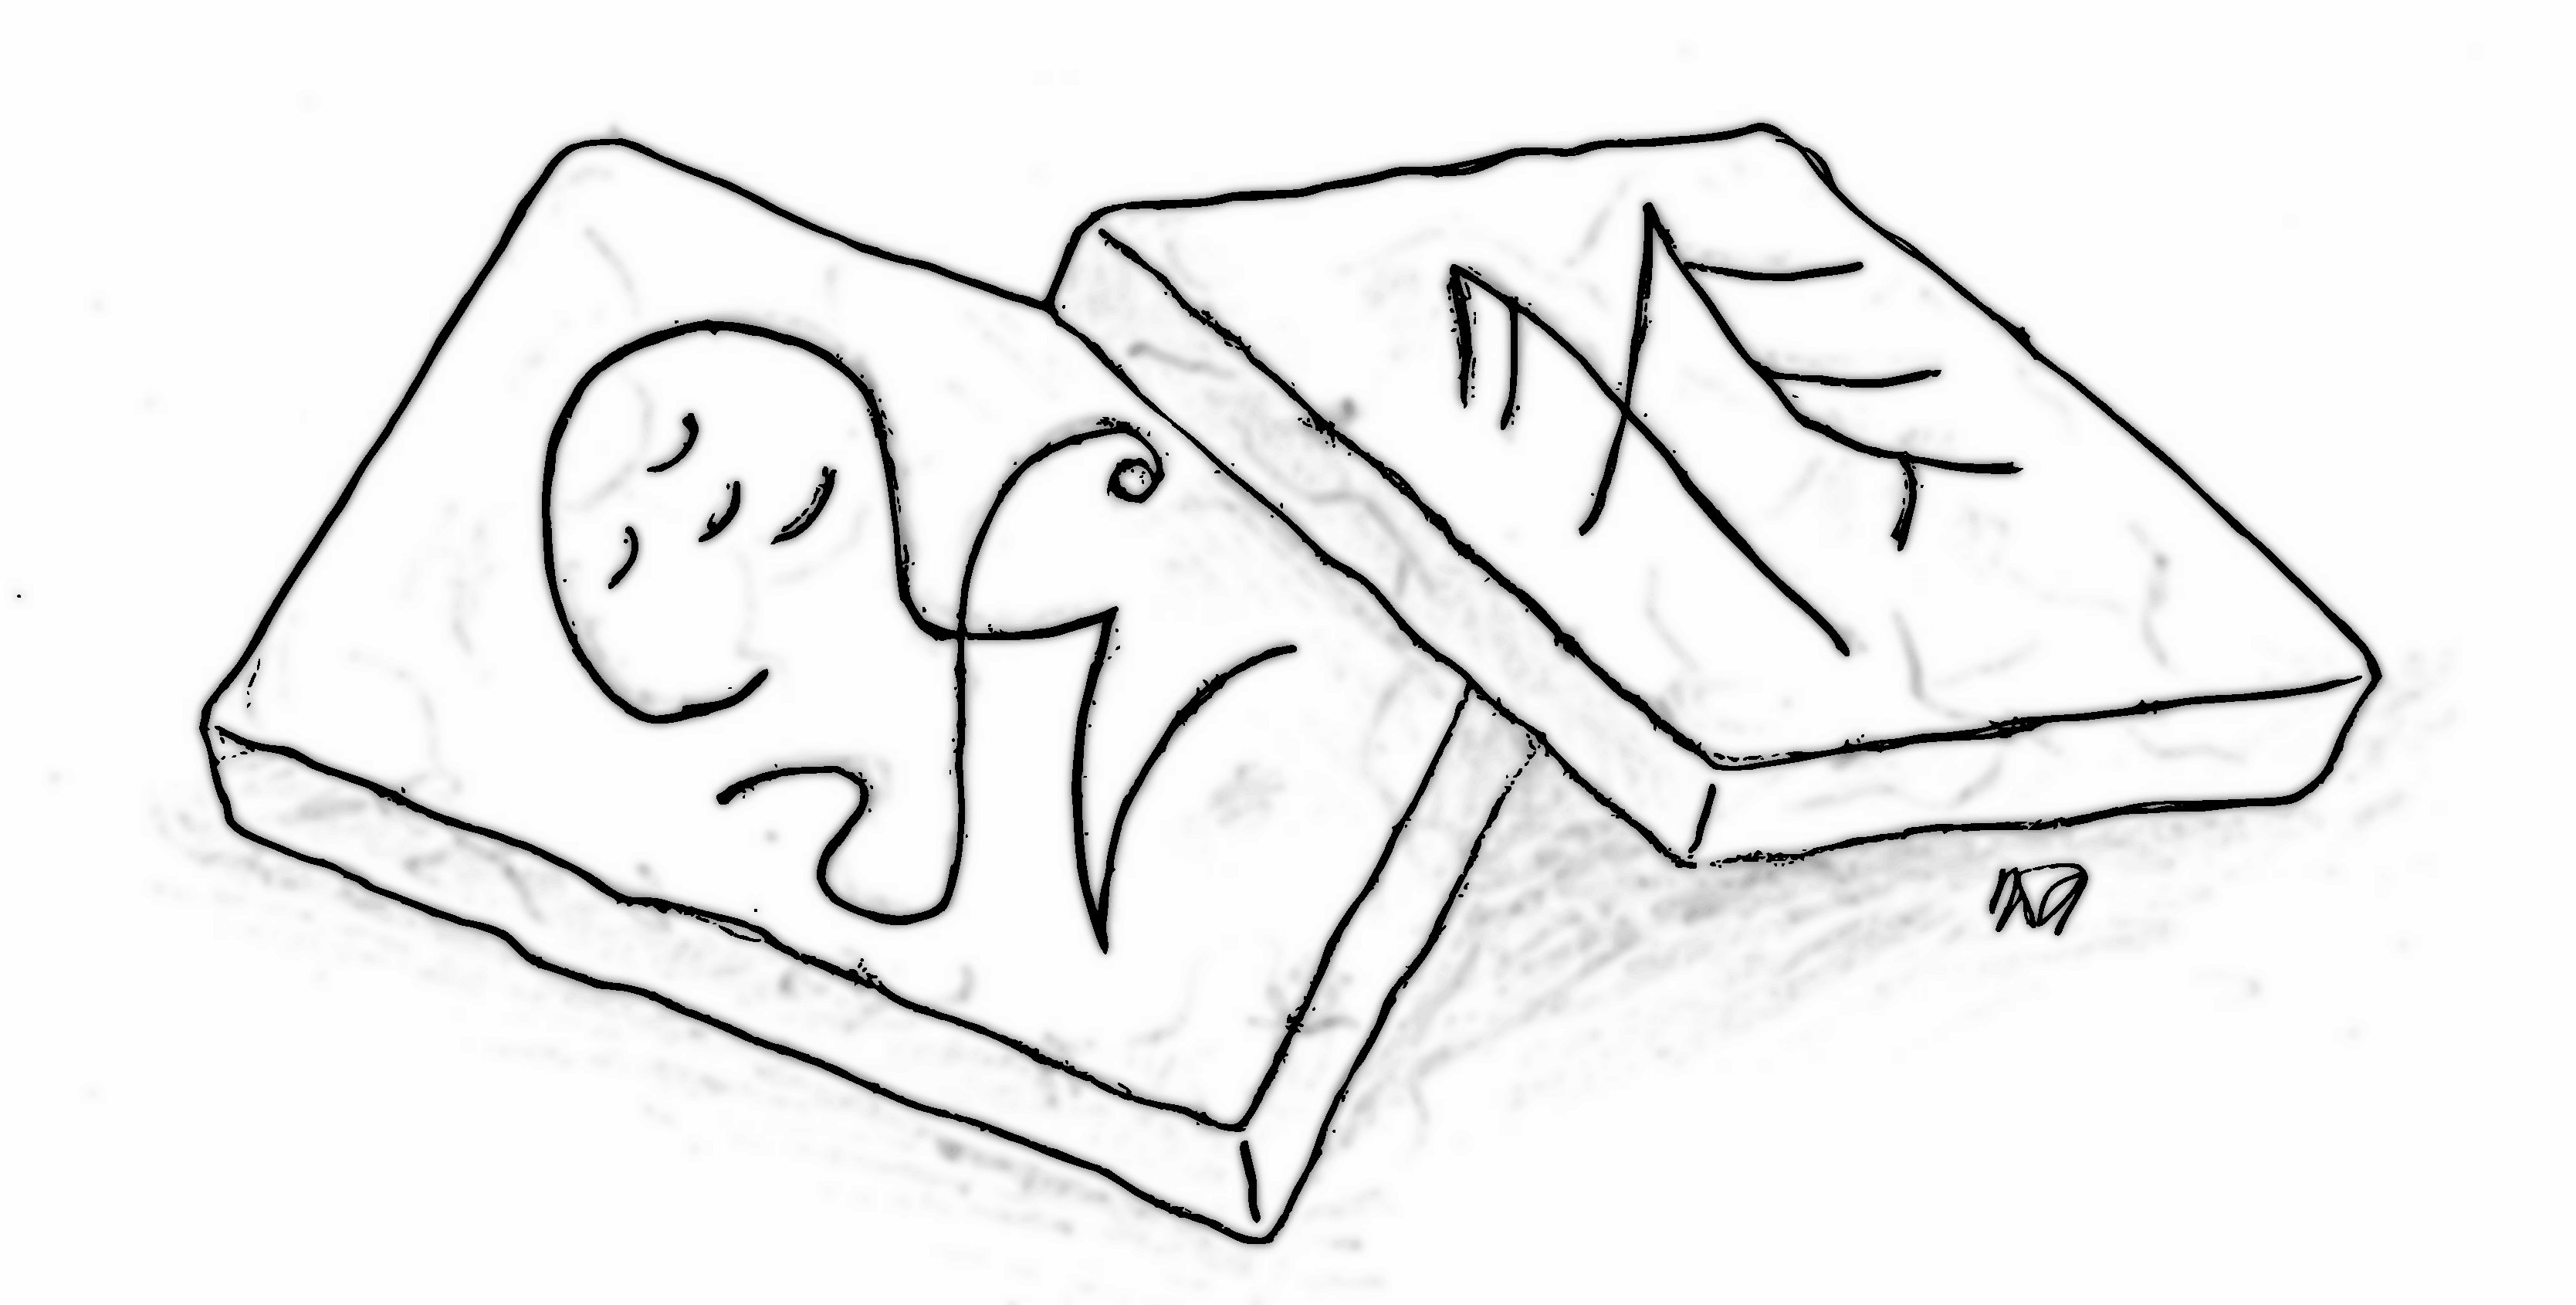
\includegraphics[width=\columnwidth]{symbol.pdf}\label{symbol}

\vspace{1em}

\noindent \textbf{\subsection{T}}

\noindent
\begin{minipage}{\columnwidth}

\noindent \textbf{Taunt (Enchantment)}

\noindent \textbf{Caster/Level:} Wizard/1

\noindent \textbf{Range:} 60 yards

\noindent \textbf{Duration:} 1 round

\noindent \textbf{Effective Area:} 30-foot radius

\noindent \textbf{Components:} V, S and M

\noindent \textbf{Casting Time:} 1

\noindent \textbf{Saving Throw:} Negate

\end{minipage}

This spell allows the caster to magically insult, irritate, anger and issue a personal challenge to any creature(s) with an intelligence of at least 2.  If the effective area contains more than one type of creature, the caster must decide which type to taunt.

The caster does not need to speak the creatures' language.  His meaning is clearly understood by all of his chosen listeners within the effective area, and they must make a successful save vs. spell, modified by wisdom---mental defense modifier, or immediately rush to attack the caster in melee combat and will not use missile attacks or spells for the spell's duration.  They move as quickly and as recklessly as possible, breaking off combat with current enemies (suffering the retreat attack) and taking the shortest route to the caster.  If they have a clear path, they'll charge (accruing both bonuses and penalties).  The presence of a strong leader (as determined by charisma score, HD/level, and other factors) may provide the victims with a saving throw bonus of up to +4, as the GM allows.  The effect immediately ends if the victim(s) are separated from the caster by an impassable boundary (such as a \textit{wall of fire}, a deep chasm, other opponent(s), etc.).  

The caster may attempt to cast this spell in conjunction with \textit{ventriloquism}.  In this case, creatures that fail their save vs. spell and became angered will then have to roll a successful intelligence check (modified as applicable for a strong leader and other factors the GM may allow).  If the intelligence check is failed, the creature rushes to attack the source of the sound, rather than the caster.

The material component is a live slug, which is thrown at the creatures to be taunted.

\vspace{1em}

\noindent
\begin{minipage}{\columnwidth}

\noindent \textbf{Telekinesis (Transmutation)}

\noindent \textbf{Caster/Level:} Wizard/5

\noindent \textbf{Range:} 10 yards/level

\noindent \textbf{Duration:} Special

\noindent \textbf{Effective Area:} Special

\noindent \textbf{Components:} V and S

\noindent \textbf{Casting Time:} 5

\noindent \textbf{Saving Throw:} Negate

\end{minipage}

This spell allows the caster to move objects or creatures mentally, simply by concentrating on them.  The spell can provide a gentle, sustained force, exert a single short, violent thrust, or if the GM allows, perform a variety of wrestling maneuvers.  The specific effect is chosen at casting time.  The effects can be countered by using an enlarge spell to make the body weight go over the maximum spell limit. The various big hand spells can also counter this spell.

\textbf{Sustained Force:}  A sustained force moves an object weighing no more than 25 pounds per caster level (maximum 375 pounds at 15th level) up to 20 feet per round.  A creature can negate the effect on an object it possesses with a successful save vs. spell, with a modifier between $-2$ and +4 depending on the conditions (such as how the object is held or worn, surprise, etc.), or with magic resistance. 

This effect lasts up to 2 rounds~+~1 round per caster level.  The object can be moved vertically, horizontally, or in both directions, but cannot be moved beyond the spell's range.  If the object is forced beyond the range, or the caster ceases concentration for any reason, the object falls or stops. 

An object can be telekinetically manipulated as if with one hand. For example, a lever or rope can be pulled, a key can be turned, an object rotated, and so on, if the force required is within the weight limitation. The caster might even be able to untie simple knots, though delicate activities such as these require intelligence checks.

\textbf{Violent Thrust:} A violent thrust expends the spell's energy in a single round.  The caster can hurl up to a total weight of 25 pounds per caster level (maximum 375 pounds at 15\textsuperscript{th} level).  The caster can hurl one object or creature per caster level directly away from his person.  Up to a maximum of 15 objects and/or creatures, within range and each within 10 feet of the next, are hurled at high speed up to 10 feet per caster level.  

Creatures who fall within the weight capacity of the spell can be hurled, but they are allowed a save vs. spell (and magic resistance) to negate the effect, as are those whose held possessions are targeted by the spell.  If a creature is telekinetically hurled against a solid surface, it takes damage as if it had fallen (1d6 points per 10 feet of distance hurled).

The caster may hurl creatures or objects at other creatures or objects.  The caster must succeed on attack rolls (one per creature or object thrown) to hit his targets, using his THACO, modified by intelligence.  Every point of intelligence above 14 adds 1, and every point below 5 subtracts 1.  Telekinetically hurled weapons cause normal damage (with no strength modifiers; note that arrows or bolts deal damage as daggers when used in this manner). Other objects cause damage ranging from 1 point per 25 pounds (for less dangerous objects) to 1d6 points of damage per 25 pounds (for hard, dense objects). 

\textbf{Wrestling Maneuver (Optional):} If the GM allows this effect in his campaign, the caster can use telekinesis to perform a wrestling maneuver upon an opponent, once per round.  Resolve these attempts as normal, without any armor penalties, and holds cannot be broken by melee attack.  Use the caster's intelligence rather than strength modifier to calculate damage (every point of intelligence above 14 adds 1).  No save is allowed against these attempts, but magic resistance applies normally.  This effect can last 1 round per caster level but ends if the caster ceases concentration.  The GM may require the caster to re-roll any results that he does not agree with or provide his own customized tables.

\vspace{1em}

\noindent
\begin{minipage}{\columnwidth}

\noindent \textbf{Telekinetic Sphere (Evocation, Transmutation)}

\noindent \textbf{Caster/Level:} Wizard/8

\noindent \textbf{Range:} 20 yards

\noindent \textbf{Duration:} 2 rounds/level

\noindent \textbf{Effective Area:} 1 foot/level diameter sphere 

\noindent \textbf{Components:} V, S and M

\noindent \textbf{Casting Time:} 4

\noindent \textbf{Saving Throw:} Negate

\end{minipage}

This spell functions as an advanced resilient sphere, and everything within the globe weighs only $^1$/$_1$$_6$ normal.  

The caster can use the globe to telekinetically move anything within it that normally weighs up to 5,000 pounds (reduced to less than 370 pounds), as either a sustained force effect or violent thrust effect, with a distance of 10 yards per caster level.  Refer to the \textit{telekinesis} spell for details regarding the sustained force and violent thrust effects.

The globe may be used to move objects and creatures heavier than 5,000 pounds manually by applying sufficient force to roll the globe at its reduced weight (370 pounds or more).  

The effect on the encapsulated victim is similar to that of a \textit{feather fall}, i.e. rapid motion, falling, or crashing the sphere into solid objects is relatively harmless to what's inside of it, however, the results could be tragic, should the spell's duration expire or the globe otherwise vanish while it is high in the air or just before it hits a solid object at high speed.  The caster can dismiss the sphere at will.

The material components are a matched set of hemispheres, one made of a hard, clear gemstone (diamond is preferred), the other of gum Arabic, as well as a small pair of bar magnets.

\vspace{1em}

\noindent
\begin{minipage}{\columnwidth}

\noindent \textbf{Teleport (Universal)}

\noindent \textbf{Caster/Level:} Wizard/5

\noindent \textbf{Range:} Touch

\noindent \textbf{Duration:} Instantaneous

\noindent \textbf{Effective Area:} Special

\noindent \textbf{Components:} V

\noindent \textbf{Casting Time:} 2

\noindent \textbf{Saving Throw:} None

\end{minipage}

This spell allows the caster to instantly transport a maximum of 250 pounds~+~150 pounds per caster level above 10\textsuperscript{th} (a 14\textsuperscript{th} level caster could \textit{teleport} a total of 850 pounds).  This includes the combined weight of his person, his gear, plus any other creatures and their gear that the caster is touching.  He can travel to any location that has something solid to stand upon, within his current plane of existence, but the caster may not arrive there safely.  The caster can do nothing else during the round he arrives from a \textit{teleport}.  The GM may determine that certain types of strong physical or magical energies block \textit{teleportation} into or out of an area or increase the chance of arriving dangerously.

Effects that block or hinder a \textit{plane shift} spell also affects the use of this spell.

The normal chances of arriving at the location safely depend on how familiar the caster is with the location.  ``Very familiar" is a place where the caster has been very often and feels at home.  ``Studied carefully" is a place the caster knows well, either because he can currently see it, has been there often, or has used other means (such as scrying) to study the place for at least one hour.  ``Seen casually" is a place that the caster has seen more than once but with which he is not very familiar.  ``Viewed once" is a place that the caster has seen only once, possibly using magic.  ``Never seen" is a place that the caster may have only seen listed on a map, or been told its exact details by someone who is very familiar with the location.

\noindent
\begin{tabular}{|p{.3\columnwidth}|p{.15\columnwidth}|p{.2\columnwidth}|p{.15\columnwidth}|}
\hline
Familiarity	& Low	& On Target	& High \\
\hline\hline
\rowcolor[gray]{.9}Very familiar	& 01	& 02--98	& 99--00 \\
Studied carefully	& 01--02	& 03--96	& 97--00 \\
\rowcolor[gray]{.9}Seen casually	& 01--04	& 05--92	& 93--00 \\
Viewed once	& 01--08	& 09--84	& 85--00 \\
\rowcolor[gray]{.9}Never seen	& 01--16	& 17--68	& 69--00 \\
\hline
\end{tabular}

If ``on target", the caster arrives safely but has no control over the direction he faces upon arrival.  Arriving ``high" indicates the caster arrives 10 feet above the ground for every 1\% he rolls above the highest ``on target" probability (up to 320 feet).  A ``low" result indicates the opposite of ``high" (as low as 160 feet).  Any result of ``high" or ``low" which \textit{teleports} the caster into mid-air results in a normal fall, while a result that \textit{teleports} the caster into a solid object almost always instantly destroys him and all that \textit{teleported} with him, though the GM may determine exceptions.  For example, \textit{teleporting} high and hitting a small tree branch may not kill everyone (at least maybe not instantly) or destroy all of the gear, but there will most likely be substantial damage.

\vspace{1em}

\noindent
\begin{minipage}{\columnwidth}

\noindent \textbf{Teleport Without Error (Universal)}

\noindent \textbf{Caster/Level:} Wizard/7

\noindent \textbf{Range:} Touch

\noindent \textbf{Duration:} Instantaneous

\noindent \textbf{Effective Area:} Special

\noindent \textbf{Components:} V

\noindent \textbf{Casting Time:} 1

\noindent \textbf{Saving Throw:} None

\end{minipage}

This spell functions as an advanced form of \textit{teleport}.  The caster is able to \textit{teleport} the same combined amount of weight, including his person, gear, any other creatures and their gear, as allowed by that spell, to anywhere within his current plane of existence without a chance of ``high" or ``low" results, even if he has never seen the location.  

The caster is also able to \textit{teleport} between the planes of existence using the same chances for error found with the \textit{teleport} spell, except that familiarity categories are reduced by one, such that the highest chance of success is ``studied carefully" and the caster cannot travel to a location on another plane that he has ``never seen".

Effects that block or hinder a \textit{plane shift} spell also affects the use of this spell.

\vspace{1em}

\noindent
\begin{minipage}{\columnwidth}

\noindent \textbf{\textit{Temporal Stasis} (Transmutation)}

\noindent \textbf{Caster/Level:} Wizard/9

\noindent \textbf{Range:} 10 yards

\noindent \textbf{Duration:} Permanent

\noindent \textbf{Effective Area:} 1 creature

\noindent \textbf{Components:} V, S and M

\noindent \textbf{Casting Time:} 9

\noindent \textbf{Saving Throw:} None

\end{minipage}

This spell allows the caster to place a creature into a state of suspended animation.  The caster must succeed on a melee touch attack against an unwilling creature.  For the creature, time ceases to flow and its condition becomes fixed (he cannot heal, rest, regain spells, etc.).  The creature does not grow older, and is not aware of its surroundings.  Its body functions virtually cease, and no force or effect can harm it.

The effects are permanent until a successful \textit{dispel magic} or the spell's reverse is cast.  

The material components are powdered diamond, emerald, ruby, and sapphire dust, where each crushed stone must be worth at least 100 gp (minimum 400 gp total).

The reverse, \textit{temporal reinstatement}, requires only a verbal component, and the caster utters but a single word to cast it.

\vspace{1em}

\noindent
\begin{minipage}{\columnwidth}

\noindent \textbf{Time Stop (Transmutation)}

\noindent \textbf{Caster/Level:} Wizard/9

\noindent \textbf{Range:} 0

\noindent \textbf{Duration:} Special

\noindent \textbf{Effective Area:} 15-foot radius

\noindent \textbf{Components:} V

\noindent \textbf{Casting Time:} 9

\noindent \textbf{Saving Throw:} None

\end{minipage}

This spell removes the caster from the normal space-time continuum by allowing him (and objects that he is touching, wearing, carrying, etc.) to enter an inter-dimensional time bubble the size of the effective area, so that time ceases to flow for all creatures everywhere, except the caster and those creatures of demigod status and higher.  The caster remains in hyper-time for what seems like 1d3 minutes, but actually takes no normal time.  The caster immediately resolves 1d3 rounds worth of actions before reverting to normal space-time.  Unless the caster brings enemies into the time-bubble (see below), this is considered a non-combat situation as far as spell casting is concerned, so most casters use the additional time to improve their defenses, summon allies, or flee from combat, but as will be seen, it can also be used to ``instantly" move objects around, save one or more allies from harm, set up an ambush, or challenge one or more opponents within the time bubble.

The caster cannot move or harm objects that are being held, carried, or worn by a creature stuck in normal space-time, but he can affect any object that is not in another creature's possession.  Objects held by those in hyper-time return to reality when released.  Objects lose all of their momentum when crossing from hyper-time to normal time, so if thrown or left in mid-air, an object just hangs there until the spell effect ends and then falls.  This makes missile weapons ineffective inside the time bubble.

Creatures outside of the time bubble cannot be attacked or targeted by a spell.  Spells with an effective area must be targeted inside the time bubble and do not damage those outside of it.  If the caster targets one or more creatures inside the time bubble with any spell or melee attack, or otherwise physically interacts with them, the creature or creatures (and the gear they carry or wear) enter hyper-time with the caster.  The caster makes his first attack as if automatically winning initiative, but otherwise the attack is resolved normally (the opponents' AC and saves remain unchanged), and the caster's opponent(s) are able to react immediately, before initiative is rolled normally or the time stop spell ends (as applicable).  Only the caster is able to interact with objects or creatures stuck in normal space-time.  If a creature that the caster has interacted with leaves the time bubble, it returns to normal space-time, but if the caster leaves the time bubble in any way (including \textit{teleport}, \textit{plane shift}, etc.), the time stop ends immediately.

Normal and magical fire, cold, gas, and similar effects that existed when the spell was cast still exist (albeit frozen in time) and can cause damage to the caster and other creatures brought into hyper-time.

The caster cannot enter an area protected by an anti-magic field while under the effect of time stop.

To prevent abuse of the spell, the GM must carefully time the caster's actions, either by calculating the game time of each of the caster's actions, or if the caster acts in ways that do not have definite times associated with them, the GM may use an egg-timer or other device to time the spell.

\noindent
\includegraphics[width=3.6in, height=1.25in]{testblock.pdf}
 
\vspace{1em}

\noindent
\begin{minipage}{\columnwidth}

\noindent \textbf{\textit{Tongues} (Transmutation)}

\noindent \textbf{Caster/Level (Sphere):} Priest/4 (All), Wizard/3

\noindent \textbf{Range:} 0

\noindent \textbf{Duration:} Priest---1 turn, Wizard---1 round/level

\noindent \textbf{Effective Area:} 60-foot radius

\noindent \textbf{Components:} Priest---V and S, Wizard---V and M

\noindent \textbf{Casting Time:} Priest---7, Wizard---3

\noindent \textbf{Saving Throw:} None

\end{minipage}

This spell allows the caster to speak and understand one additional language per three caster levels.  The caster need not name a specific language but can simply target one or more creatures, within the effective area, that he wishes to communicate with.  

All such creatures within the effective area understand the caster, but the creature(s) are not necessarily friendly or cooperative.  The GM may wish to roll an encounter reaction check, modified by the caster's charisma---reaction modifier.  The caster cannot use this spell to speak with animals or mindless creatures.  

The reverse, \textit{confuse tongues}, disrupts all conversation within the effective area, or can be used to cancel the effects of a \textit{tongues} spell.

The material component for both the spell and its reverse is a small model of a ziggurat made of clay, which the caster shatters while casting the spell.

The priests' version of this spell functions as the wizard spell of the same name, except there is no material component.

 
\vspace{1em}

\noindent
\begin{minipage}{\columnwidth}

\noindent \textbf{Transmute Metal to Wood (Transmutation)}

\noindent \textbf{Caster/Level (Sphere):} Priest/7 (Elemental (Earth))

\noindent \textbf{Range:} 80 yards

\noindent \textbf{Duration:} Permanent

\noindent \textbf{Effective Area:} 1 metal object

\noindent \textbf{Components:} V, S and M

\noindent \textbf{Casting Time:} 1 round

\noindent \textbf{Saving Throw:} Special

\end{minipage}

This spell allows the caster to transform a metal object of up to 10 pounds per caster level within range into one made of wood.  Metal objects with magical properties gain a 90\% resistant to the effect, and objects carried, held or worn by a creature receive a saving throw equal to the creature's save vs. spell.  Artifacts and relics cannot be affected by this spell.  Only a \textit{limited wish}, \textit{wish} or similar effect will restore the object to its original form.  

Weapons converted from metal to wood suffer a $-2$ penalty on attack and damage rolls, and they splinter and break on any natural attack roll of 1 or 2.  Armor converted from metal to wood suffers a +2 AC penalty and an additional armor class penalty every time it is struck with a natural attack roll of 19 or 20.

The material component is the caster's holy or unholy symbol.

\vspace{1em}

\noindent
\begin{minipage}{\columnwidth}

\noindent \textbf{\textit{Transmute Rock to Mud} (Transmutation)}

\noindent \textbf{Caster/Level (Sphere):} Priest/5 (Elemental (Earth, Water)), Wizard/5

\noindent \textbf{Range:} Priest---160 yards, Wizard---10 yards/level

\noindent \textbf{Duration:} Special

\noindent \textbf{Effective Area:} Up to two 10-foot cubes/level

\noindent \textbf{Components:} V, S and M

\noindent \textbf{Casting Time:} Priest---8, Wizard---5

\noindent \textbf{Saving Throw:} None

\end{minipage}

This spell allows the caster to transform natural, uncut rock of any sort, in the effective area and within range, into an equal volume of mud.  Magical or enchanted stone is not affected by the spell.  Rocks or stones in the possession of a creature gain a saving throw equal to the creature's save vs. spell.  The depth of the mud cannot exceed 10 feet.  

Tiny-sized or smaller creatures, those specially adapted for movement on top of the mud, and those able to levitate, fly, or otherwise get free from the mud, can avoid ill effect.  Small-sized or larger creatures (up to 10' tall) sink $^1$/$_3$ of their height each round, until they are chest-deep, hip-deep, and finally completely submerged by the end of the third round.  While partially submerged, a creature moves at a speed of 1, and suffers a $-2$ penalty on its attack rolls and a +2 penalty to its AC.  A completely submerged creature can no longer move or attack effectively and may suffocate unless rescued (Refer to Holding A Character's Breath).  Large, heavy creatures, over 10' tall, sink all the way to the bottom and can wade through the effective area as if partially submerged.

Brush thrown atop the mud can support creatures able to climb on top of it, however, the GM must adjudicate the exact results.
 
If transmute rock to mud is cast upon the ceiling of a cavern or tunnel, the mud falls to the floor and spreads out in a pool at a depth of 5 feet. The falling mud and the ensuing cave-in deal 8d6 points of bludgeoning damage to anyone caught directly beneath the effective area, or half damage to those who successfully save vs. spell, modified by their dexterity---surprise modifier. 

Castles and large stone buildings are generally immune to the effect of the spell, since transmute rock to mud can't affect worked stone and doesn't reach deep enough to undermine such buildings' foundations.  However, small buildings or structures often rest upon foundations shallow enough to be damaged or even partially toppled by this spell's effect. 

The mud remains until a successful \textit{dispel magic} or \textit{transmute mud to rock} restores its substance--but not necessarily its form. Evaporation turns the mud into normal dirt over a period of days. The exact time depends on exposure to the sun, wind, and normal drainage, with a rate of 1d6 days per 10 cubic feet being average.

The material components are clay and water.

The reverse, \textit{transmute mud to rock}, transforms normal mud or quicksand into soft stone (sandstone or similar mineral) permanently, until a successful \textit{dispel magic} or \textit{transmute rock to mud} is cast.  Creatures in the mud are allowed a saving throw, modified by dexterity---surprise modifier, to escape before the area hardens into stone. Dry sand is unaffected.

The material components for the reverse are sand, lime, and water.

The priests' versions of this spell and its reverse function as the wizards' spell of the same name (including material components).

\vspace{1em}

\noindent
\begin{minipage}{\columnwidth}

\noindent \textbf{\textit{Transmute Water to Dust} (Transmutation)}

\noindent \textbf{Caster/Level (Sphere):} Priest/6 (Elemental (Water, Earth)), Wizard/6

\noindent \textbf{Range:} 60 yards

\noindent \textbf{Duration:} Permanent

\noindent \textbf{Effective Area:} Priest---1 cubic yard/level, Wizard---10-foot cube/level

\noindent \textbf{Components:} V, S and M

\noindent \textbf{Casting Time:} Priest---8, Wizard---5

\noindent \textbf{Saving Throw:} None (Special)

\end{minipage}

This spell allows the caster to transform an amount of water-based liquid, up to the effective area and within range, into fine dust.  Only the watery component of the liquid is affected, however if cast on muddy water, the effective area is doubled, and if wet mud is used, the effective area is quadrupled.  If sufficient water still exists after the spell's casting, it soaks the dust, creating a silt-laden mud.  The dust is magical and can be dispelled in the first round of its creation, after which it becomes normal, mundane dust.  If this spell is cast on a single, unattended potion, the potion is permanently ruined.  A potion in a creature's possession is allowed a saving throw equal to the creature's save vs. spell.  

This spell does not affect most creatures, although it can be cast on a single creature from the Elemental Plane of Water, inflicting 1d6 points of damage per caster level.  The creature is allowed to roll a saving throw vs. spell to reduce the damage by half. 

The material components are diamond dust worth at least 500 gp and a bit of seashell.

The reverse, \textit{transmute dust to water}, acts as an extremely powerful \textit{create water} spell, creating clean water in the effective area.  The water is magical and can be dispelled in the first round of its creation, after which it becomes normal, mundane water.

The material components for the reverse are diamond dust worth at least 500 gp and a bit of seashell, and a pinch of dust.

The priests' version of this spell and its reverse functions as the wizards' spell of the same name (including material components), except that it slays a creature from the Elemental Plane of Water, unless a successful save vs. spell is rolled.  A successful save inflicts 1d6 points of damage per caster level.

\vspace{1em}

\noindent
\begin{minipage}{\columnwidth}

\noindent \textbf{Transport Via Plants (Transmutation)}

\noindent \textbf{Caster/Level (Sphere):} Priest/6 (Plant)

\noindent \textbf{Range:} Touch

\noindent \textbf{Duration:} Special

\noindent \textbf{Effective Area:} Special

\noindent \textbf{Components:} V and S

\noindent \textbf{Casting Time:} 4

\noindent \textbf{Saving Throw:} None

\end{minipage}

This spell allows the caster to enter any normal plant (man-sized or larger) and exit a second plant of the same kind in a single round, regardless of the distance separating the two.  The caster cannot use this spell to travel through plant-based creatures.  The entry plant must be alive.  The destination plant need not be familiar to the caster, but it also must be alive.  If a particular destination plant is desired, but that plant is not living, the spell fails and the caster must leave the entry plant within 24 hours or he is ejected.  If the caster is uncertain of the location of a particular destination plant, he merely needs to designate direction and distance and he will be moved as close as possible to the desired location, usually within 1 mile, but there's a 20\%~$-$~1\% per caster level chance of being transported to a plant 1d100 miles away from his desired destination.

The caster can bring along objects as long as their combined weight doesn't exceed his strength---max weight score.  He may also bring one additional willing man-sized or smaller creature (carrying gear or objects up to its strength---max weight score) or its equivalent per three caster levels.  Use the following equivalents to determine the maximum number of larger creatures that the caster can bring along: A large creature counts as two man-sized creatures, and a huge creature counts as two large creatures, etc.  All creatures to be transported must be in contact with one another, and at least one of those creatures must be in contact with the caster.  Unwilling creatures gain a save vs. spell to avoid the being taken along.

The destruction of an occupied plant slays the caster and any creatures that he has brought along, and ejects the bodies and all carried objects.


\vspace{1em}

\noindent
\begin{minipage}{\columnwidth}

\noindent \textbf{Trap the Soul (Conjuration)}

\noindent \textbf{Caster/Level:} Wizard/8

\noindent \textbf{Range:} 10 yards

\noindent \textbf{Duration:} Permanent

\noindent \textbf{Effective Area:} 1 specific creature

\noindent \textbf{Components:} V, S and M

\noindent \textbf{Casting Time:} Special

\noindent \textbf{Saving Throw:} Special

\end{minipage}

This spell allows the caster to imprison a creature's life force (whether it be a soul or spirit) and its material body (as applicable) within a specially prepared gem.  In some ways, this spell acts as an advanced form of the magic jar spell.

The caster chooses a gem specifically for the creature that he intends to trap.  It must be a flawless gem, cut by a master gem-cutter, worth at least 1,000 gp per HD or level of the creature.  The gem is then prepared by casting enchant an item followed by a maze spell, which permanently forms a prison within it.  

If successful, the gem traps the creature indefinitely or until broken, releasing the life force and allowing the material body to reform.  While trapped, the creature is aware of its surroundings outside the gem, but does not age, nor does it feel the need to eat, breathe or sleep.  The creature can go free once the gem is broken, unless it is from another plane (including creatures from the Prime Material trapped on other planes).  In this case, the creature that broke the gem can require the trapped creature to perform a service immediately upon being freed.  However, as with magic jar, long-term entrapment may cause long-term or permanent insanity, and the GM must adjudicate the results.

There are two triggering methods, one of which is chosen when the spell is memorized. 

\textbf{Spell Completion (Verbal):} The caster can trigger the effect by speaking the spell's final verbal component while the subject is in range, as if he were casting a regular spell with a casting time of 1.  The target is allowed a saving throw and magic resistance check to avoid the effect.  If the creature's true name is spoken as well, magic resistance is ignored and the creature suffers a $-2$ penalty on its saving throw.  If the save or magic resistance check is successful, the gem shatters. 

\textbf{Spell Completion (Written):} The second method is far more insidious, for it tricks the subject into accepting an object inscribed with the final verbal spell component.  The caster must inscribe both the creature's true name and the final verbal component upon the object while preparing the gem.  A sympathy spell can also be placed on the object at any time.  As soon as the subject picks up or accepts the object (even if done under the influence of charm or other enchantments), its life force is automatically transferred to the gem without the benefit of magic resistance or a save.

The material component for this spell is the prepared gem.  If the gem isn't valuable enough to contain the creature, the spell fails and the gem shatters during the casting.  While creatures have no concept of level or Hit Dice as such, the value of the gem needed to trap an individual can be researched.  This value can change over time if the creature gains more Hit Dice (or levels).

%\noindent
\includegraphics[width=3.3in, height=1.5in]{testblock.pdf} 

\vspace{1em}

\noindent
\begin{minipage}{\columnwidth}

\noindent \textbf{Tree (Transmutation)}

\noindent \textbf{Caster/Level (Sphere):} Priest/3 (Plant)

\noindent \textbf{Range:} 0

\noindent \textbf{Duration:} 6 turns~+~1 turn/level

\noindent \textbf{Effective Area:} The caster

\noindent \textbf{Components:} V, S and M

\noindent \textbf{Casting Time:} 6

\noindent \textbf{Saving Throw:} None

\end{minipage}

This spell allows the caster, along with all of the gear he is wearing and carrying, to take the form of either a small living tree or shrub, or a large, dead tree trunk.  The caster is aware of his surroundings and retains his current AC, saves and hit points while in tree form, however, in other mundane ways, he cannot be distinguished from a genuine tree.  If properly detected for, the caster radiates his alignment and a faint aura of magic (transmutation), while in tree form.

The caster can end the spell before the duration expires by reverting to his normal form at the beginning of a round.  The caster is then able to roll initiative and act normally during the rest of that round.

The material component is the caster's holy or unholy symbol and a twig from a tree.

\vspace{1em}

\noindent
\begin{minipage}{\columnwidth}

\noindent \textbf{Trip (Enchantment)}

\noindent \textbf{Caster/Level:} Priest/2 (Plant)

\noindent \textbf{Range:} Touch

\noindent \textbf{Duration:} 1 turn/level

\noindent \textbf{Effective Area:} 1 object up to 10 ft. long

\noindent \textbf{Components:} V and S

\noindent \textbf{Casting Time:} 5

\noindent \textbf{Saving Throw:} Negate

\end{minipage}

This spell allows the caster to enchant an otherwise mundane length of vine, stick, pole, rope, or similar long slender object to rise slightly off the ground and attempt to trip all creatures that cross over it, including the caster, until the duration expires.  The enchanted object can be discovered as if it were a magical trap (via rogue's ability, detect traps, detect snares and pits, etc.), but is otherwise 80\% undetectable.  The other 20\% of the time, a careful observer will see the object move as he or someone crosses over it.  A successful save vs. spell avoids the effect, otherwise the creature trips, falls and has a 50\% chance to drop whatever it is carrying.  The GM may decide that dropped items must make a saving throw to avoid being damaged or ruined.  Getting back on their feet (and picking up any dropped items) consumes a full round.  If a creature is aware of the object before it crosses over, it gains a +4 bonus to its saving throw and only has a 25\% to drop what it is carrying.  

For every 3 feet of material the spell is cast upon, 2 small-sized or 1 man-sized creature can be tripped each round, and when it is cast upon a 10-foot long object, up to 6 small-sized, 3 man-sized, or 1 large-sized creature can be tripped each round.  Huge-sized and larger creatures are immune to the effects, but they can still trigger the trap.

Creatures that are running when tripped suffer 1d4~+~1 hit points of damage and are stunned for the same number of rounds, if they fall on hard ground, but suffer only 1 hit point of damage and are stunned for only one round if the ground is soft.  The spell does not function underwater.

\vspace{1em}

\noindent
\begin{minipage}{\columnwidth}

\noindent \textbf{\textit{True Seeing} (Greater Divination)}

\noindent \textbf{Caster/Level (Sphere):} Priest/5 (All), Wizard/6

\noindent \textbf{Range:} Touch

\noindent \textbf{Duration:} 1 round/level

\noindent \textbf{Effective Area:} 1 creature

\noindent \textbf{Components:} V, S and M

\noindent \textbf{Casting Time:} Priest---8, Wizard---1 round

\noindent \textbf{Saving Throw:} None

\end{minipage}

This spell allows the caster to confer upon the subject the ability to see all things as they actually are.  The caster may choose to be the subject.  The subject sees through normal and magical darkness (seeing those hiding in shadows), notices secret and magically hidden doors, sees the exact locations of creatures or objects under blur or displacement effects, sees invisible creatures or objects normally, sees through illusions, and sees the true form of polymorphed, changed, or transmuted things  (the true form appears as a translucent outline superimposed over the image).  Furthermore, once per round, the subject can adjust its vision to see into the Ethereal (including out-of-phase), Astral or other adjacent planes.  The GM may allow this spell to see into an inter-dimensional space, like a \textit{rope trick}, but not into a non-planar space, like a \textit{portable hole}.  The range of true seeing conferred is 60 feet. 

\textit{True seeing}, however, does not penetrate solid objects. It in no way confers X-ray vision or its equivalent.  It does not negate concealment, including that caused by fog and the like.  \textit{True seeing} does not help the viewer see through mundane disguises, spot creatures who are simply hiding behind something, or notice secret and concealed doors hidden by mundane means.  In addition, the spell effects cannot be further enhanced with known magic, so one cannot use \textit{true seeing} through a \textit{crystal ball} or in conjunction with \textit{clairaudience} or \textit{clairvoyance}. 

The material component is an eye ointment made from powdered mushroom, saffron, and fat, costing at least 300 gp per dose and then aged for 1d6 months.

The priests' version of this spell functions as the wizards' spell of the same name (including its material component) with the following exceptions:  It is reversible, the caster's vision range is 120 feet, and the caster is able to see a creature's aura and determine its alignment.  

The reverse, \textit{false seeing}, provides the caster with a limited ability to falsify what the subject sees for the spell's duration.  An unwilling victim must be struck with a successful touch attack, however, trickery is often used to gain unknowing and therefore willing victims.  The caster mentally influences the subject to think it sees something different than what its eyes actually report.  The caster cannot make the subject see something that is not there, nor make the subject completely oblivious to something, but he can replace the appearance of one thing with another.  For instance, he could make a human look like a dwarf (or one human look like another specific human), a closed door look like it is open, a vat of acid look like rose water, a parrot look like a bookend, stale rations look like fresh fruit, a light pat on the back look like a dagger thrust, etc. 

The caster cannot alter the apparent size of a creature or object by more than 50\%. Thus, he cannot make a castle look like a hovel, but he could make it look like a different castle or a rough hillock, whether smaller, larger or of approximately the same size. 

Because the caster is overriding the victim's senses, he can fool a victim who is using \textit{true seeing} or some other method of gathering information, assuming he knows that the victim is actively using such an effect and concentrates for the spell's duration.

The material component for the reverse is an eye ointment made from oil, poppy dust, and pink orchid essence, costing at least 300 gp per dose and then aged for 1d6 months.

\vspace{1em}

\noindent
\begin{minipage}{\columnwidth}

\noindent \textbf{Turn Wood (Transmutation)}

\noindent \textbf{Caster/Level (Sphere):} Priest/6 (Plant)

\noindent \textbf{Range:} 0

\noindent \textbf{Duration:} 1 round/level

\noindent \textbf{Effective Area:} 20 feet/level~$\times$~120 feet wide

\noindent \textbf{Components:} V and S

\noindent \textbf{Casting Time:} 9

\noindent \textbf{Saving Throw:} None

\end{minipage}

This spell allows the caster to project waves of force in the direction that he faces, which cause all wooden objects in the path of the effective area to be forced away from him to the limit of the effective area.  Loose objects are repelled at the rate of 40 feet per round.  Wooden objects larger than 3 inches in diameter that are fixed firmly are not affected, but loose objects are.  Objects 3 inches in diameter or smaller (such as spears) that are fixed in place splinter and break, and the pieces move with the wave of energy. 

Objects such as wooden shields, spears, wooden weapon shafts and hafts, and arrows and bolts are pushed back, dragging those carrying them along.  A creature being dragged by an item it is carrying can let go.  Even magic items with wooden sections are repelled, although an anti-magic field blocks the effects. 

The waves of force continue to sweep down the set path for the spell's duration. After the spell is cast, the path is set, and the caster can do other things or go elsewhere without affecting the spell's power.  A successful \textit{dispel magic} will end the effect.

\vspace{1em}

\noindent \textbf{\subsection{U}}

\noindent
\begin{minipage}{\columnwidth}

\noindent \textbf{Uncontrollable Hideous Laughter (Enchantment)}

\noindent \textbf{Caster/Level:} Wizard/2

\noindent \textbf{Range:} 60 yards

\noindent \textbf{Duration:} 1 round/level

\noindent \textbf{Effective Area:} 30-foot cube

\noindent \textbf{Components:} V, S and M

\noindent \textbf{Casting Time:} 2

\noindent \textbf{Saving Throw:} Negate

\end{minipage}

This spell allows the caster to afflict one creature per 3 caster levels, in range and within the effective area, with uncontrollable laughter.  Unless a saving throw versus spell is successful, each creature starts to believe that everything it sees and hears is uproariously hilarious.  The saving throw is modified by intelligence.  Creatures with an intelligence score of 4 or less are unaffected, those with intelligence of 5--7 save with a $-6$ penalty, those with intelligence of 8--12 save with a $-4$ penalty, those with intelligence of 13--14 save with a $-2$ penalty, and those with intelligence of 15 or more save normally.  If the creature fails its save, it immediately stops whatever it is doing and begins to chuckle.  Finally, the creature collapses into gales of manic laughter by the end of the 1\textsuperscript{st} round.  The laughing continues during the 2\textsuperscript{nd} round.  The creature must then spend the 3\textsuperscript{rd} round regaining its feet.  For each remaining round of the spell's duration (if any), the creature can act normally, but suffers a 2 points penalty to its strength score.  The GM applies a $-2$ penalty to attack and damage rolls if a creature's strength is unknown.

The material components are a feather and miniature tarts.  The caster throws the tarts at the creature(s) and waves the feather in one hand.

\noindent
\includegraphics[width=3.6in, height=2.5in]{testblock.pdf}

\vspace{1em}

\noindent
\begin{minipage}{\columnwidth}

\noindent \textbf{Unseen Servant (Conjuration)}

\noindent \textbf{Caster/Level:} Wizard/1

\noindent \textbf{Range:} 0

\noindent \textbf{Duration:} 1 hour~+~1 turn/level

\noindent \textbf{Effective Area:} 30-foot radius

\noindent \textbf{Components:} V, S and M

\noindent \textbf{Casting Time:} 1

\noindent \textbf{Saving Throw:} None

\end{minipage}

This spell allows the caster to create an invisible, mindless, shapeless force that performs simple tasks at his command.  It can step and fetch things, open unstuck doors, and hold chairs, as well as clean and mend.  It can open only normal doors, drawers, lids, etc.  The servant can perform only one activity at a time, but it will repeat the same activity over and over again if told to do so.  It can lift 20 pounds or push/pull 40 pounds.  It can trigger traps and such, but it can exert only 20 pounds of force, which is not enough to activate certain pressure plates and other devices.  It can't perform any task that requires training to learn.  Its movement value is 3, but it cannot run.

The servant cannot attack in any way; it is never allowed an attack roll.  It cannot be killed but dissipates if a successful \textit{dispel magic} is cast upon it, or if it takes 6 points of damage in a single round from attacks with effective areas.  It gets no saves against these attacks.  In addition, if the caster attempts to send it beyond the spell's effective area (measured from the caster's current position), the servant will cease to exist. 

The material components are small amounts of string and wood.

\vspace{1em}

\noindent \textbf{\subsection{V}}

\noindent
\begin{minipage}{\columnwidth}

\noindent \textbf{Vacancy (Transmutation, Illusion)}

\noindent \textbf{Caster/Level:} Wizard/4

\noindent \textbf{Range:} 10 yards/level

\noindent \textbf{Duration:} 1 hour/level

\noindent \textbf{Effective Area:} 10-foot radius/level

\noindent \textbf{Components:} V, S and M

\noindent \textbf{Casting Time:} 4

\noindent \textbf{Saving Throw:} None

\end{minipage}

This potent spell allows the caster to combine invisibility and illusion effects to make any location (up to the size of the effective area) appear to be completely vacant, unused and abandoned for a long period of time.  The illusion has visual, auditory, olfactory, and thermal components, but it is most effective when used indoors or underground.  The GM must adjudicate the results in outdoor wilderness settings.
 
Those who pass through the effective area will see dirt and dust, feel cobwebs, smell mold, and otherwise believe it to be a typical, empty location.  They see their own tracks in the dust, and think they are ripping away cobwebs, etc.  It cannot disguise, conceal, or add creatures, however, it will appear as if they too have just discovered the vacant area.  Only fresh tracks appear in the dust (as appropriate), with no other trace of the creature(s) being there for longer than a few minutes.  

The spell cannot alter the appearance of structures (or add them where none are present).  All furnishings and objects within the effective area are made invisible.  If a creature makes forceful contact with an invisible object (such as running into a statue or something, finding smaller objects on a tabletop, etc.), it naturally becomes suspicious and is granted a saving throw to disbelieve the entire effect.  A successful save allows the viewer to see the location as it truly is and provide a +4 bonus to their allies' saves (Refer to Illusions).  If a creature fails the save, it will conclude that the object(s) it has found are simply invisible.  A successful \textit{dispel magic} cast over the entire location will end the spell effect, but when cast upon an individual object only reveals that object.  Otherwise, objects made invisible will remain invisible for the entire duration, even if removed from the effective area.  \textit{True seeing}, or similar can see through the illusion, but detect invisibility will only reveal objects already discovered. 

The material component is a square of fine black silk worth at least 100 gp.

\vspace{1em}

\noindent
\begin{minipage}{\columnwidth}

\noindent \textbf{Vampiric Touch (Necromancy)}

\noindent \textbf{Caster/Level:} Wizard/3

\noindent \textbf{Range:} 0

\noindent \textbf{Duration:} One touch

\noindent \textbf{Effective Area:} The caster

\noindent \textbf{Components:} V and S

\noindent \textbf{Casting Time:} 3

\noindent \textbf{Saving Throw:} None

\end{minipage}

This spell allows the caster to channel negative energy inflicting 1d6 hit points of damage per two caster levels with a successful touch attack (up to a maximum of 6d6).  As soon as a successful touch attack is scored or one turn passes, the spell effect ends.  The damage can be healed by any normal mundane or magical method.  The caster gains hit points equal to the damage he inflicts (up to the amount required to kill the victim).  Hit points above the caster's normal maximum are temporary.  Temporary hit points not already lost disappear after 1 hour.

The undead cannot be negatively affected by this spell.

\vspace{1em}

\noindent
\begin{minipage}{\columnwidth}

\noindent \textbf{Vanish (Transmutation)}

\noindent \textbf{Caster/Level:} Wizard/7

\noindent \textbf{Range:} Touch

\noindent \textbf{Duration:} Special

\noindent \textbf{Effective Area:} 1 object

\noindent \textbf{Components:} V

\noindent \textbf{Casting Time:} 2

\noindent \textbf{Saving Throw:} None

\end{minipage}

This spell allows the caster to cause an object to ``go away".  The spell only affects one inanimate object, which the caster must be touching for the entire casting time.  It cannot affect artifacts, relics, creatures, constructs, accursed items or magical forces.  The object must be both no more than 50 pounds per caster level and no larger than 3 cubic feet per caster level.  If the caster targets an object that surpasses either one of these limitations, the spell fails. 

This spell can have one of two effects, chosen at the time of casting.  There is a 1\% chance that the object \textit{disintegrates} when the spell is cast upon it regardless of which effect is chosen, no save granted.

\textbf{Teleport Object:} The caster causes the object to reappear at a desired location, as if it had been \textit{teleported} (Refer to \textit{Teleport}, including chances for arriving high or low).

\textbf{Hide Object:} The caster hides the object deep in the Ethereal Plane.  The spot where the object was located will permanently radiate a faint aura of magic until a successful \textit{dispel magic} cast upon that spot returns the object.  There's a 1\% chance that a creature from the Ethereal Plane can use the object's link to travel to the Prime Material.  A check is made when the object is sent away, once per day while it abides there, and once more when it is returned.  No less than 3 checks will be made.

\vspace{1em}

\noindent
\begin{minipage}{\columnwidth}

\noindent \textbf{Veil (Illusion)}

\noindent \textbf{Caster/Level:} Wizard/6

\noindent \textbf{Range:} 10 yards/level

\noindent \textbf{Duration:} 1 turn/level

\noindent \textbf{Effective Area:} 20-foot cube/level

\noindent \textbf{Components:} V and S

\noindent \textbf{Casting Time:} 6

\noindent \textbf{Saving Throw:} None

\end{minipage}

This spell acts as a more powerful version of \textit{hallucinatory terrain}, allowing the caster to instantly change the appearance of a location and/or any creatures, within range and the effective area, whether the setting is indoors or outdoors.  The illusion has visual, auditory, olfactory, tactile and thermal components, and retains that appearance for the spell's duration.  The caster can make the location and/or its occupants appear to be any combination of things he desires.  Creatures resume their normal appearances if slain.  

Unlike most other illusions, this one is so convincing that only \textit{true seeing} or similar effects will reveal the hallucinatory terrain portion of the effect.  This portion of the illusion cannot be disbelieved.  Creatures who do not desire to have their appearance altered may make a save vs. spell or by magic resistance (as applicable).  Those who interact with an affected creature may gain a save to disbelieve that part of the illusion, modified by wisdom---mental defense modifier, but magic resistance will not help.  

\vspace{1em}

\noindent
\begin{minipage}{\columnwidth}

\noindent \textbf{Ventriloquism (Illusion)}

\noindent \textbf{Caster/Level:} Wizard/1

\noindent \textbf{Range:} 10 yards/level, 90 yards maximum

\noindent \textbf{Duration:} 4 rounds~+~1 round/level

\noindent \textbf{Effective Area:} 1 creature or object

\noindent \textbf{Components:} V and M

\noindent \textbf{Casting Time:} 1

\noindent \textbf{Saving Throw:} Negate

\end{minipage}

This spell allows the caster to make his voice (or any sound that he can normally make vocally) seem to issue from someplace else within range.  The caster can speak in any language he knows.  Anyone who hears the sound and rolls a successful save, modified by wisdom---mental defense modifier and a $-2$ penalty, recognizes it as illusory (but still hears it).  \textit{Ventriloquism} can be combined with other illusory effects.  Doing so reduces the penalties or provides bonuses to the save as determined by the GM. 

The material component is a parchment rolled up into a small cone.

\vspace{1em}

\noindent
\begin{minipage}{\columnwidth}

\noindent \textbf{Vision (Greater Divination)}

\noindent \textbf{Caster/Level:} Wizard/7

\noindent \textbf{Range:} 0

\noindent \textbf{Duration:} Special

\noindent \textbf{Effective Area:} The caster

\noindent \textbf{Components:} V, S and M

\noindent \textbf{Casting Time:} 7

\noindent \textbf{Saving Throw:} None

\end{minipage}

This spell is similar to \textit{contact other plane}.  The caster requests supernatural guidance from a power of his choice, and is allowed to ask a question that is answered with a vision.  The chances that the power provides a useful vision is determined by a 2d6 roll (with appropriate modifiers for using a valuable material component---see below).

\noindent
\begin{tabular}{|p{.12\columnwidth}|p{.78\columnwidth}|}
\hline
2d6	& Result \\
\hline\hline
\rowcolor[gray]{.9}2--6	& The power is annoyed and refuses to answer the question.  The power demands a service from the caster in the form of a \textit{geas} that even a \textit{wish} cannot remove. \\
7--9	& The power is indifferent and answers with a minor vision.  The vision is not necessarily directly related to the question, but will provide at least one clue. \\
\rowcolor[gray]{.9}10--12	& The power is pleased and grants a fully detailed vision specifically answering the question, but the caster will need to interpret the vision properly. \\
\hline
\end{tabular}

The material component is an item that the caster values or is valued by the power being contacted.  The caster sacrifices the item to the power during the casting of the spell.   Items valued at 5,000 gp or more grant a +1 bonus to the 2d6 results roll.  Those valued at 25,000 gp or more grant a +2 to the roll, while those valued at 50,000 gp or more grant the maximum bonus of +3.

\vspace{1em}

\noindent \textbf{\subsection{W}}

\noindent
\begin{minipage}{\columnwidth}

\noindent \textbf{Wall of Fire (Evocation)}

\noindent \textbf{Caster/Level (Sphere):} Priest/5 (Elemental (Fire)), Wizard/4

\noindent \textbf{Range:} Priest---80 yards, Wizard---60 yards

\noindent \textbf{Duration:} Special

\noindent \textbf{Effective Area:} Special

\noindent \textbf{Components:} V, S and M

\noindent \textbf{Casting Time:} Priest---8, Wizard---4

\noindent \textbf{Saving Throw:} None

\end{minipage}

This spell allows the caster to create an immobile, blazing curtain of shimmering reddish-blue fire.  The effective area can be formed into either an opaque sheet of flames up to one 20 foot square per caster level or a ring of fire with a radius up to 10 feet~+~5 feet per two caster levels.  In either form, the wall is vertical with respect to the caster's angle and 20 feet high.  The wall lasts for as long as the caster concentrates or one round per caster level thereafter.

One side of the wall, selected by the caster, sends forth waves of heat, dealing 2d4 points of damage to creatures within 10 feet and 1d4 points of damage to those past 10 feet but within 20 feet.  The wall inflicts this damage when it appears and on his initiative each round to all creatures in the area.  In addition, the wall deals 2d6 points of damage~+~1 point of damage per caster level (maximum~+~20) to any creature passing through it.  The wall deals double damage to the undead. 

If the caster evokes the wall so that it appears where basically stationary creatures are, each creature takes damage as if passing through the wall, however, creating a wall to intentionally catch and cause damage to a moving creature grants a saving throw to allow it to escape the effective area before the wall forms.  The moving creature may take subsequent damage normally if it remains inside the effective area when the caster gains his next initiative.

If any 5-foot section of the wall takes 20 points or more of damage from cold attacks in a single round, that section goes out.  \textit{Wall of fire} can be made permanent with a \textit{permanency spell}.  A permanent \textit{wall of fire} that is extinguished by cold damage becomes inactive for a turn, and then reforms at normal strength.

The priests' version of this spell functions as the wizards' spell of the same name except that the flames are yellowish-green in color, and creatures passing through the wall suffer 4d4 points of damage~+~1 per caster level.  

The material component for both priests' and wizards' versions is phosphorus.

\vspace{1em}

\noindent
\begin{minipage}{\columnwidth}

\noindent \textbf{Wall of Fog (Evocation)}

\noindent \textbf{Caster/Level:} Wizard/1

\noindent \textbf{Range:} 30 yards

\noindent \textbf{Duration:} 2d4 rounds~+~1 round/level

\noindent \textbf{Effective Area:} 20-foot cube~+~10-foot cube/level

\noindent \textbf{Components:} V, S and M

\noindent \textbf{Casting Time:} 1

\noindent \textbf{Saving Throw:} None

\end{minipage}

This spell allows the caster to create billowy clouds of misty vapors within the spell's range that form a wall up to the effective area in size.  The fog obscures all normal vision and infravision beyond 2 feet.  The wall must be a cube or rectangular-shaped, and at least 10 feet across at its smallest point.  The duration is halved by a moderate wind and a strong wind immediately ends the spell effects.

The material component is a pinch of split, dried peas.

\noindent
\includegraphics[width=3.6in, height=2.5in]{testblock.pdf}

\vspace{1em}

\noindent
\begin{minipage}{\columnwidth}

\noindent \textbf{Wall of Force (Evocation)}

\noindent \textbf{Caster/Level:} Wizard/5

\noindent \textbf{Range:} 30 yards

\noindent \textbf{Duration:} 1 turn~+~1 round/level

\noindent \textbf{Effective Area:} Special

\noindent \textbf{Components:} V, S and M

\noindent \textbf{Casting Time:} 5

\noindent \textbf{Saving Throw:} None

\end{minipage}

This spell allows the caster to create an invisible, immobile wall anywhere within range.  The caster can either form the wall into a flat wall made of one 10 foot~$\times$~10 foot square per level, a sphere with a radius up to 1 foot per caster level, or into a hemisphere with a radius of 1.5 feet per caster level.  The wall must be continuous and unbroken.  If any object or creature breaks the wall's surface while it is being created, the spell fails.  The wall blocks ethereal creatures as well as material ones, but \textit{dimension door}, \textit{teleport}, and similar effects can bypass the barrier, and ethereal creatures can usually get around a flat wall or hemispherical form by floating under it or around it through the material floors, walls or ceilings.  Creating a wall to intentionally capture a creature grants a saving throw, modified by dexterity---surprise modifier, to allow it to escape before the wall forms.  

Breath weapons and spells cannot pass through the wall in either direction, but gaze attacks can operate through a \textit{wall of force}.  The wall is immune to damage of any kind and is unaffected by most spells, including \textit{dispel magic}.  However, \textit{disintegrate} immediately destroys it, as does a \textit{rod of cancellation}, a \textit{sphere of annihilation}, or a successful \textit{mage's disjunction} spell, and the caster can end the effect before the duration expires with a command word.

\textit{Wall of force} can be made permanent with a \textit{permanency spell}.  If brought down by \textit{disintegrate}, \textit{mage's disjunction} or other powerful effect, a permanent \textit{wall of force} will return after 1 turn. 

The material component is a pinch of powdered diamond worth 5,000 gp.

\vspace{1em}

\noindent
\begin{minipage}{\columnwidth}

\noindent \textbf{Wall of Ice (Evocation)}

\noindent \textbf{Caster/Level:} Wizard/4

\noindent \textbf{Range:} 10 yards

\noindent \textbf{Duration:} 1 turn/level

\noindent \textbf{Effective Area:} Special

\noindent \textbf{Components:} V, S and M

\noindent \textbf{Casting Time:} 4

\noindent \textbf{Saving Throw:} Special

\end{minipage}

This spell allows the caster to create a barrier made of ice.  The wall must be continuous and unbroken.  If any object or creature breaks the wall's surface while it is being created, the spell fails. 

This spell can create one of three effects, chosen at the time of casting.

\textbf{Ice Plane:} This effect creates a sheet of strong, hard ice, which lasts for the duration, it is melted or until a successful \textit{dispel magic} is cast.  The wall is 1 inch thick per caster level.  It covers up to a 10-foot-square area per caster level (so a 10\textsuperscript{th}-level wizard can create a \textit{wall of ice} 100 feet long and 10 feet high, a wall 50 feet long and 20 feet high, or some other combination of length and height that does not exceed 1,000 square feet).  The plane can be oriented in any fashion as long as it is anchored.  A vertical wall need only be anchored on the floor, while a horizontal or slanting wall must be anchored on two opposite sides.   It is possible, but difficult, to trap a mobile opponent with an ice plane, provided the ice forms to block the only way out.  Creating an ice plane to intentionally capture a creature grants a saving throw, modified by dexterity---surprise reaction modifier, to allow it to escape before the wall forms.

Each 10-foot square of wall has 3 hit points per inch of thickness.  Creatures can hit the wall automatically.  A section of wall whose hit points drop to 0 is breached, but an area of frigid air remains.  If a creature passes through the breach in the ice, it suffers 2 points of damage per inch of thickness of the wall.  Fire-based creatures suffer 3 points of damage per inch, and cold-based creatures suffer only 1 point of damage per inch when going through.  Magical fire (including fiery breath weapons and spell effects of 3\textsuperscript{rd} level or better) melts an ice plane in one round, but doing so creates a steamy fog 10 times larger than the spell's effective area, which acts as if it were a \textit{wall of fog} spell for one turn.  Lesser spell effects and normal fires do not affect the wall.

\textbf{Hemisphere:} This effect creates a hemisphere with a maximum radius of 3 feet plus 1 foot per caster level, which lasts until it is broken, melted, or a successful \textit{dispel magic} is cast.  Magical fire (including fiery breath weapons and spell effects of 3\textsuperscript{rd} level or better) melts the hemisphere in one round, but doing so creates a steamy fog 10 times larger than the spell's effective area, which acts as if it were a \textit{wall of fog} spell for one turn.  Lesser spell effects and normal fires do not affect the hemisphere.

The hemisphere is just as thick and as hard to break through as the ice plane form, but it does not deal damage to those who go through a breach.  It can be used to trap immobile creatures, but creating a wall to intentionally catch a moving creature grants a saving throw, modified by dexterity---surprise modifier, to allow it to escape before the wall forms.

\textbf{Hail Storm:} The final effect does not create a barrier; rather it functions as an ice storm's hail effect for one round, in an effective area of 10-foot square per caster level.  The fallen ice remains on the ground for the spell's duration, a successful \textit{dispel magic} is cast or until it is melted with magical fire.  Melting the effects of the hail storm does not create an effective fog.

The material component for all three of the effects is the same: a small piece of a quartz or similar rock crystal.

\vspace{1em}

\noindent
\begin{minipage}{\columnwidth}

\noindent \textbf{Wall of Iron (Evocation)}

\noindent \textbf{Caster/Level:} Wizard/5

\noindent \textbf{Range:} 5 yards/level

\noindent \textbf{Duration:} Permanent

\noindent \textbf{Effective Area:} Special

\noindent \textbf{Components:} V, S and M

\noindent \textbf{Casting Time:} 5

\noindent \textbf{Saving Throw:} None

\end{minipage}

This spell allows the caster to cause a flat, vertical iron wall to spring into being.  The wall inserts itself into any surrounding non-living material (to seal off a passage, for instance) if its effective area is sufficient to do so.  The wall must be continuous and unbroken.  If any object or creature breaks the wall's surface while it is being created, the spell fails.  It must always be a flat plane, though the caster can shape its edges to fit the available space.   It is possible, but difficult, to trap a mobile opponent with a wall of iron, provided the wall forms to block the only way out.  Creating a wall to intentionally capture a creature grants a saving throw, modified by dexterity---surprise modifier, to allow it to escape.

A wall of iron is $^1$/$_4$ inch thick and 15 square feet per caster level.  The caster is allowed to double the wall's effective area by halving its thickness.  Each 5-foot square of the wall has 30 hit points per inch of thickness.  A section of wall whose hit points drop to 0 is breached.  

If the caster desires, the wall can be created vertically resting on a flat surface but not attached to the surface, so that it can be tipped over to fall on and crush creatures beneath it.  The wall is 50\% likely to tip in either direction if left alone.  Creatures can attempt to push the wall in one direction rather than letting it fall randomly.  If a combined strength of at least 30 or a combined mass of 400 pounds pushes against it, each pound over 400 and/or point of strength over 30 increases the chance of falling toward the weaker side by 1\%.  Creatures with room to flee the falling wall may do so by making successful save vs. death, modified by dexterity---surprise modifier.  Any large-sized or smaller creature that fails is instantly crushed to death. The wall cannot crush huge-sized and larger creatures. 

The wall is permanent until a successful \textit{dispel magic} is cast but is otherwise normal, non-magical iron.  Like any iron wall, this wall is subject to rust, perforation, and other natural phenomena.

The material component is a small piece of sheet iron.

\vspace{1em}

\noindent
\begin{minipage}{\columnwidth}

\noindent \textbf{Wall of Stone (Evocation)}

\noindent \textbf{Caster/Level:} Wizard/5

\noindent \textbf{Range:} 5 yards/level

\noindent \textbf{Duration:} Permanent

\noindent \textbf{Effective Area:} Special

\noindent \textbf{Components:} V, S and M

\noindent \textbf{Casting Time:} 5

\noindent \textbf{Saving Throw:} None

\end{minipage}

This spell allows the caster to create a wall of granite that merges into adjoining rock surfaces.  A \textit{wall of stone} is $^1$/$_4$ inch thick and up to 20 square feet per caster level.  The caster is allowed to double the wall's effective area by halving its thickness.  The wall must be continuous and unbroken.  If any object or creature breaks the wall's surface while it is being created, the spell fails.   

Unlike a \textit{wall of iron}, the caster is allowed to create a \textit{wall of stone} in almost any shape desired.  The wall need not be vertical, nor rest upon any firm foundation; however, it must merge with and be solidly supported by existing stone.  It can be used to bridge a chasm, for instance, or as a ramp.  For this use, if the span is more than 20 feet, the wall must be arched and buttressed.  This requirement reduces the spell's effective area by half.  The wall can be crudely shaped to allow crenellations, battlements, and so forth by likewise reducing the effective area. 

The wall is permanent until a successful \textit{dispel magic} is cast but is otherwise normal, non-magical stone.  Like any other wall made of stone, this one can be destroyed by a \textit{disintegrate} spell or by normal means such as breaking and chipping.  Each 5-foot square of the wall has 15 hit points per inch of thickness.   A section of wall whose hit points drop to 0 is breached.  

It is possible, but difficult, to trap a mobile opponent within or under a \textit{wall of stone}, provided the wall is shaped so it can hold the creature.  Creating a wall to intentionally capture a creature grants a saving throw, modified by dexterity---surprise modifier, to allow it to escape.

The material component is a small block of granite.

\vspace{1em}

\noindent
\begin{minipage}{\columnwidth}

\noindent \textbf{Wall of Thorns (Conjuration)}

\noindent \textbf{Caster/Level (Sphere):} Priest/6 (Plant, Creation)

\noindent \textbf{Range:} 80 yards

\noindent \textbf{Duration:} 1 turn/level

\noindent \textbf{Effective Area:} Special

\noindent \textbf{Components:} V and S

\noindent \textbf{Casting Time:} 9

\noindent \textbf{Saving Throw:} None

\end{minipage}

This spell allows the caster to create a barrier of very tough, pliable, tangled brush bearing needle-sharp thorns as long as a human's finger (about 3 inches).  Only the nearest edge of the wall must be within range.  The caster can form the wall into any basic shape he desires, up to one 10-foot cube per caster level or two 10-foot by 10-foot by 5-foot blocks per caster level.  The effect lasts for the duration, until a successful \textit{dispel magic} is cast or until the caster dismisses it.

Creatures with the ability to pass through overgrown areas unhindered can pass through a \textit{wall of thorns} at normal speed without taking damage.  Otherwise, a creature forced into or attempting to move through a \textit{wall of thorns} takes slashing damage per round of movement equal to 8 plus the creature's AC (up to a maximum of 18 damage per round).  A negative AC reduces the damage taken, until an AC of $-8$ reduces the damage to 0.  Dexterity modifiers to AC do not count for this calculation.  

Creating a wall to intentionally capture a creature grants a saving throw, modified by dexterity---surprise modifier, to allow it to escape unharmed.  A failed save indicates the creature is caught in the effective area and takes damage as if it had been forced into the wall.  In order to escape, it must attempt to force its way through the wall, or it can wait until the spell ends.  A creature can force its way slowly through the wall by making a strength check.  It can perform no other actions while moving through the thorns.  For every point below the score required to succeed the strength check, a creature moves 1 foot (up to a maximum distance equal to its normal land speed).  Of course, moving through or attempting to move through the thorns incurs damage as above.  Damage is checked for each 10 foot of thickness or fraction thereof a creature attempts to move through.  A creature trapped in the thorns can choose to remain motionless in order to avoid taking damage.  A 5-foot thick wall inflicts the same damage as a 10-foot wall; however, breaking through the 5-foot wall takes half as much time.  

A \textit{wall of thorns} can be breached from the outside by slow work with edged weapons.  Each person chopping away at the wall creates a 10-foot deep by 3-foot wide safe passage for every 4 turns of effort.  A 5-foot thick wall only requires 2 turns.  Magical fire (including fiery breath weapons and spell effects of 3\textsuperscript{rd} level or better) burns a wall of thorns, but doing so causes it to act as if it were a \textit{wall of fire} spell for two turns (the cool side always faces the caster of the wall of thorns spell).  Lesser spell effects and normal fires do not affect the wall.  

Despite its appearance, a wall of thorns is not actually a living plant, and thus is unaffected by spells that affect plants.

\vspace{1em}

\noindent
\begin{minipage}{\columnwidth}

\noindent \textbf{\textit{Warp Wood} (Transmutation)}

\noindent \textbf{Caster/Level (Sphere):} Priest/2 (Plant)

\noindent \textbf{Range:} 10 yards/level

\noindent \textbf{Duration:} Permanent

\noindent \textbf{Effective Area:} Special

\noindent \textbf{Components:} V and S

\noindent \textbf{Casting Time:} 5

\noindent \textbf{Saving Throw:} Special

\end{minipage}

This spell allows the caster to cause wooden items within range to bend and warp, permanently destroying their straightness, form, and strength.  A warped door springs open or becomes stuck, requiring a Strength check to open, at the caster's option.  A boat or ship can be made to spring a leak.  Warped missile weapons are useless.  A warped melee weapon causes a $-4$ penalty on attack rolls. 

The caster may warp a 15-inch shaft of wood up to 1-inch diameter or its equivalent per caster level.  At 3\textsuperscript{rd} level, the caster is able to warp 2 or 3 hand-axe handles or a dozen crossbow bolts, and at 5\textsuperscript{th} level, he can warp the shaft of a typical spear.  The caster can combine multiple consecutive castings to warp an object that is too large for him to warp with a single spell.  Until the object is completely warped, it suffers no ill effects.

Enchanted items made of wood (such as magically held doors, temporary magical weapons, etc.) can be affected only if the caster is higher level than the caster who enchanted it.  Permanent magical items made of wood are treated as if a caster of at least 12\textsuperscript{th} level enchanted them.  The spell has a 20\% cumulative chance of success per caster level higher than the level of the caster who enchanted the wood.  Artifacts and relics cannot be affected by this spell.

The reverse, \textit{straighten wood}, warps the same quantity of wood back to normal, straightening wood that has been warped either by this spell or other means. 

\vspace{1em}

\noindent
\begin{minipage}{\columnwidth}

\noindent \textbf{\textit{Water Breathing} (Transmutation)}

\noindent \textbf{Caster/Level (Sphere):} Priest/3 (Elemental (Water, Air)), Wizard/3

\noindent \textbf{Range:} Touch

\noindent \textbf{Duration:} Priest---1 hour/level, Wizard---1 hour/level~+~1d4 hours

\noindent \textbf{Effective Area:} 1 creature

\noindent \textbf{Components:} Priest---V and S, Wizard---V, S and M

\noindent \textbf{Casting Time:} Priest---6, Wizard---3

\noindent \textbf{Saving Throw:} None

\end{minipage}

This spell allows the caster to empower one or more creatures touched (which may or may not include the caster) to breathe water for the spell's duration.  Divide the duration evenly among all the creatures touched.  The spell does not make creatures unable to breathe air.

The reverse, \textit{air breathing}, enables water-breathing creatures to also breathe air.

The material component for the spell and its reverse is a short reed or piece of straw.

The priests' version of this spell, and its reverse, functions as the wizards' spell of the same name, except there is no material component.

\vspace{1em}

\noindent
\begin{minipage}{\columnwidth}

\noindent \textbf{Water Walk (Transmutation)}

\noindent \textbf{Caster/Level (Sphere):} Priest/3 (Elemental (Water))

\noindent \textbf{Range:} Touch

\noindent \textbf{Duration:} 1 turn~+~1 turn/level

\noindent \textbf{Effective Area:} Special

\noindent \textbf{Components:} V, S and M

\noindent \textbf{Casting Time:} 6

\noindent \textbf{Saving Throw:} None

\end{minipage}

This spell allows the caster to empower one creature touched plus one additional creature per caster level above 5\textsuperscript{th} (which may or may not include the caster) to tread on any liquid as if it were firm ground for the spell's duration.  Mud, oil, snow, quicksand, running water, ice, and even lava can be traversed easily, since the subjects' feet hover an inch or two above the surface on a thin, invisible field of force under the wearer.  Creatures crossing molten lava still take damage from the heat because they are near it.  The subject(s) can walk, run, charge, or otherwise move across the surface as if it were normal ground.  The subject(s) of the spell leaves depressions the size of his feet and 1$^1$/$_2$ inch deep per 100 pounds of weight in snow, quicksand or other semi-solid surfaces, caused by the field of force.  If the spell is cast underwater (or while the subject(s) are partially or wholly submerged in whatever liquid they are in), subjects that desire to go to the surface rise at a rate of 120 feet per round, while those who are dead, unconscious, more than lightly encumbered, or unwilling to go to the surface rise at a rate of only 60 feet per round, until they can stand on the surface.  The spell's subject(s) must also treat liquids as solid objects for the purpose of falling.  

The material components are a piece of cork and the caster's holy or unholy symbol.

\vspace{1em}

\noindent
\begin{minipage}{\columnwidth}

\noindent \textbf{Weather Summoning (Conjuration)}

\noindent \textbf{Caster/Level (Sphere):} Priest/6 (Weather)

\noindent \textbf{Range:} 0

\noindent \textbf{Duration:} Special

\noindent \textbf{Effective Area:} Special

\noindent \textbf{Components:} V and S

\noindent \textbf{Casting Time:} 1 turn

\noindent \textbf{Saving Throw:} None

\end{minipage}

This spell allows the caster to invoke severe weather conditions.  The caster can alter the wind speed, precipitation, and temperature to any extreme for the region and season.  This includes tornadoes, thunderstorms, ice storms, or hot weather in the spring, torrential rains, heat waves, or hailstorms in the summer, hot or cold weather, fog, or ice in the autumn, and extreme cold, blizzards, or a fast thaw in the winter.  If cast in coastal regions during late winter or early spring the caster may invoke a hurricane.

The GM must determine the spell's effective area and its duration.  The GM may consult the control weather spell for more specific weather details; however, the effects are always at or beyond the extreme ends of the scales.  The changes to the weather conditions start to become noticeable within 1d4 turns, and reach their full strength in 1d12~+~5 turns.  Depending on the severe weather conditions desired, the effective area might be between 1 and 100 square miles and the duration (after the effect has reached full strength) may be just 1 turn or up to a few days.  The caster determines which type of extreme weather is desired, but otherwise has no control over the weather that arrives and cannot change his mind once it has been called.  If a successful \textit{dispel magic} is cast at the location the \textit{weather summoning} spell was cast, before the severe weather reaches its full strength, the weather slowly reverts back to normal, however once it reaches its full strength it can no longer be dispelled.  

Several casters working in concert (either through the use of a combine spell or by casting similar complimentary spells, such as control weather, control winds, etc.) can invoke the most extreme and/or unlikely weather conditions, such as frost and snow during the summer or a heat wave in the winter.

\vspace{1em}

\noindent
\begin{minipage}{\columnwidth}

\noindent \textbf{Web (Evocation)}

\noindent \textbf{Caster/Level:} Wizard/2

\noindent \textbf{Range:} 5 yards/level

\noindent \textbf{Duration:} 2 turns/level

\noindent \textbf{Effective Area:} 8,000 cubic feet

\noindent \textbf{Components:} V, S and M

\noindent \textbf{Casting Time:} 2

\noindent \textbf{Saving Throw:} Negate or Half

\end{minipage}

This spell allows the caster to create many-layers of strong, sticky strands, similar to spider webs but far larger and tougher.  The \textit{web} covers a maximum area of eight 10~$\times$~10~$\times$~10 foot cubes and must be at least 10 feet thick.  The webs must be anchored to two or more solid and diametrically opposed points, such as floor and ceiling or opposite walls, or else the \textit{web} collapses and disappears.  

Creatures caught within a \textit{web} become entangled among the gluey fibers.  Any creature in the effective area when the spell is cast must make a save vs. spell, modified by dexterity---surprise modifier and a $-2$ penalty.  

If the save fails, the creature is entangled.  Creatures with strength score of 12 or less are trapped and unable move or perform any actions until freed by another creature or the spell's duration expires.  Creatures with strength between 13 and 17 can break through 1 foot of web per round, and those with strength above 17 break through 2 feet per round.  Huge creatures or those with great mass can move through 10 feet of webs per round, while creatures larger than huge ignore the webs completely.

If the save succeeds and the creature is adjacent to at least 5 feet of clear space, it avoids the effect entirely, but if insufficient clear space is available, the \textit{web} affects the creature at half strength.  Creatures with strength score of 7 or less are trapped and unable move or perform other actions until freed by another creature or the spell's duration expires.  Creatures with strength between 7 and 12 can break through 1 foot of half-strength web per round, and all other movement values while entangled (listed above) are doubled.

Entangled creatures (whether at full or half strength) lose any dexterity bonuses to their AC until they leave the effective area, however, missiles weapons are less effective against those trapped in the \textit{web}.  If at least 5 feet of web lie between the attacker and the entangled opponent, it provides 25\% cover.  10 feet provides 50\% cover, 15 feet provides 75\% cover and 20 feet of web or more provides 90\% cover.

In addition, using a melee weapon or other tool to attack a creature entangled in a web, or to hack at the webs to free an ally, may cause the attacker (or rescuer) to become entangled.  If less than 5 feet of web lie between the attacker/rescuer and the entangled creature, the attacker/rescuer makes a save vs. spell, modified by dexterity---surprise modifier.  If the save fails, he is entangled at half strength.  If more than 5 feet of web exists, a failed save indicates he is fully entangled, and if more than 10' feet exists, he suffers the additional -2 penalty to the save.

The strands of a \textit{web} spell are flammable. A magical flaming sword can slash them away as easily as a hand brushes away cobwebs. Any fire can set the webs alight and burn away a 10-foot cube per round.  All creatures within flaming parts of the web take 2d4 points of fire damage from the flames. 

This spell can be made permanent with a \textit{permanency} spell.  A permanent \textit{web} is stationary, and if damaged or destroyed it reforms in the same location.  Permanent \textit{webs} close in behind those who hack through them in one round and return in 1 turn if destroyed by fire.  Pieces of the web dissolve in just a few seconds if they are removed from the spell's effective area.

The material component is a bit of spider web.

\vspace{1em}

\noindent
\begin{minipage}{\columnwidth}

\noindent \textbf{Weird (Illusion)}

\noindent \textbf{Caster/Level:} Wizard/9

\noindent \textbf{Range:} 30 yards

\noindent \textbf{Duration:} Concentration

\noindent \textbf{Effective Area:} 20-foot radius

\noindent \textbf{Components:} V and S

\noindent \textbf{Casting Time:} 9

\noindent \textbf{Saving Throw:} Special

\end{minipage}

This spell is similar to \textit{phantasmal killer}, except the caster can select any number of potential victims, within the effective area, that he is able to communicate with.  While casting this spell, the caster threatens his intended victims with impending doom in whatever language(s) they can understand.  

The selected creatures must roll a saving throw vs. spell, modified by wisdom---mental defense modifier.  

Those who fail the save are suddenly involved in a seemingly real battle with phantasmal images culled from their darkest subconscious.  The GM must adjudicate the phantasmal monsters, but in general, each phantasmal monster shares the caster's Level/HD, and possibly other stats.  Escape of any sort (including \textit{teleport}, \textit{plane shift}, etc.) is impossible.  In reality, the victims are paralyzed, and the combat is only occurring within their minds.  Combat begins immediately, but each round of this mental combat takes only $^1$/$_1$$_0$ of an actual round.  If the mental combat reaches 1 turn (1 round of actual time), initiative is rolled for all others who are not affected by the spell.  Those creatures under the effects of the spell can be attacked and suffer damage, but they cannot be brought out of the mental combat until the spell ends or they have successfully defeated the phantasmal monster.  If the victim dies in mental combat, he dies in reality, but if he defeats the phantasmal monster, the spell ends.  The victim revives unharmed, and he has not used any actual equipment or spells.  He also gains experience for defeating the phantasm.  

An affected creature sees only the phantasmal monster attacking it but not those attacking others.  The caster must concentrate to maintain the phantasms.  The spell ends if the caster loses concentration.

Those victims who successfully save are paralyzed with fear for a full round and lose 1d4 points of strength, but do not face a phantasmal monster.  If a creature does not have a known strength the GM may instead assign $-$1d4 in combat penalties.  The victim's strength returns after 1 turn.  If a creature that saved successfully is attacked and sustains damage while paralyzed with fear, the paralysis effect ends and they can react immediately, albeit with a lowered strength score.  

\vspace{1em}

\noindent
\begin{minipage}{\columnwidth}

\noindent \textbf{Whispering Wind (Transmutation, Illusion)}

\noindent \textbf{Caster/Level:} Wizard/2

\noindent \textbf{Range:} 1 mile/level

\noindent \textbf{Duration:} Special

\noindent \textbf{Effective Area:} 2-foot radius

\noindent \textbf{Components:} V and S

\noindent \textbf{Casting Time:} 2

\noindent \textbf{Saving Throw:} None

\end{minipage}

This spell allows the caster to send a message or a sound on the wind to a designated spot.  The \textit{whispering wind} travels to a specific location within range that is familiar to the caster, provided that it can find a way to the location.  A \textit{whispering wind} is as gentle and unnoticed as a zephyr until it reaches the location.  It then delivers its whisper-quiet message or other sound.  Note that the message is delivered regardless of whether anyone is present to hear it.  The wind then dissipates. 

The caster can prepare the spell to bear a message of no more than twenty-five words, cause the spell to deliver other sounds for 1 round, or merely have the whispering wind seem to be a faint stirring of the air.  He can likewise cause the \textit{whispering wind} to move as slowly as 1 mile per hour or as quickly as 1 mile per turn. 

When the spell reaches its objective, it swirls and remains in place until the message is delivered.  As with \textit{magic mouth}, \textit{whispering wind} cannot speak verbal components, use command words, or activate magical effects.

\vspace{1em}

\noindent
\begin{minipage}{\columnwidth}

\noindent \textbf{Wind Walk (Transmutation)}

\noindent \textbf{Caster/Level (Sphere):} Priest/7 (Elemental (Air))

\noindent \textbf{Range:} Touch

\noindent \textbf{Duration:} 1 hour/level

\noindent \textbf{Effective Area:} The caster~+~1 person per 8 levels

\noindent \textbf{Components:} V, S and M

\noindent \textbf{Casting Time:} 1 round

\noindent \textbf{Saving Throw:} None

\end{minipage}

This spell allows the caster to alter the substance of his body and everything worn or carried to a cloudlike vapor (as a \textit{potion of gaseous form}) and move through the air, possibly at great speed.  The caster can take a maximum of up to three other creatures with him.  A magic wind allows them to move at a rate as slow as 6 with maneuver class of 1, up to 20 with a maneuver class of 2, up to 40 with a maneuver class of 3, up to 60 with maneuver class of 4, and as fast as 60 mph (or 1 mile per round) if flying at or above altitudes of 600 feet with only maneuverability necessary for long distance traveling.  

Wind walkers are not invisible but rather appear misty and translucent.  If fully clothed in white, they are 80\% likely to be mistaken for clouds, fog, vapors, etc.  A wind walker can regain its physical form as desired and later resume the cloud form.  Each change to or from vaporous form requires 1 full round, which counts toward the duration of the spell (as does any time spent in physical form).  The caster can dismiss the effect completely and for everyone at once, or he can dismiss it for individual wind walkers and not others. 

During the last round of the spell's duration, a wind walker in cloud form automatically descends as much as 600 feet in order to land.  This rapid descent serves as a warning that the spell is about to end.

While in vapor form, creatures are immune to attacks from normal weapons.  No spell casting is possible while in vapor form.  Winds may allow a wind walker to move faster than 60 mph if blowing from behind, and move at a slower speed or have difficulty navigating if blowing against them.  Wind speeds of tornado strength and higher will completely impede travel in that direction.

The material components are fire and holy or unholy water.

\columnbreak

\vspace{1em}

\noindent
\begin{minipage}{\columnwidth}

\noindent \textbf{Wind Wall (Transmutation)}

\noindent \textbf{Caster/Level:} Wizard/3

\noindent \textbf{Range:} 10 yards/level

\noindent \textbf{Duration:} 1 round/level

\noindent \textbf{Effective Area:} 10 feet~$\times$~5 feet/level, 2 feet wide

\noindent \textbf{Components:} V, S and M

\noindent \textbf{Casting Time:} 3

\noindent \textbf{Saving Throw:} Special

\end{minipage}

This spell allows the caster to create an invisible vertical curtain of wind, 2 feet thick and of considerable strength.  It is a roaring blast of upward wind sufficient to blow away any bird smaller than an eagle, or tear papers and similar materials from unsuspecting hands.  A save vs. spell, modified by dexterity---surprise modifier, allows a creature to maintain its grasp on an object.  Small-sized and smaller flying creatures cannot pass through the barrier.  Loose materials and clothing fly upward when caught in a wind wall.  Arrows, bolts and sling stones are deflected upward and miss, while any other hurled weapon passing through the wall suffers a $-4$ penalty to the first shot and $-2$ penalty to further shots.  A giant-thrown boulder, a siege engine projectile, and other massive ranged weapons are not affected.  Gases, most gaseous breath weapons, and creatures in gaseous form cannot pass through the wall, but it poses no barrier to incorporeal creatures. 

While the wall must be vertical, the caster can shape it in any continuous path along the ground that he likes.  It is possible to create cylindrical or square \textit{wind walls} to enclose specific locations.

The material components are a tiny fan and a feather from an exotic creature.

\vspace{1em}

\noindent
\begin{minipage}{\columnwidth}

\noindent \textbf{Wish (Conjuration, Evocation)}

\noindent \textbf{Caster/Level:} Wizard/9

\noindent \textbf{Range:} Unlimited

\noindent \textbf{Duration:} Special

\noindent \textbf{Effective Area:} Special

\noindent \textbf{Components:} Special

\noindent \textbf{Casting Time:} Special

\noindent \textbf{Saving Throw:} Special

\end{minipage}

This spell allows the caster to alter reality to better suit him.  It is the mightiest spell a wizard can cast, and like \textit{limited wish}, can require GM and player adjudication.  It can have any of several effects chosen at casting time.

\index{Races!and Wishes}\textbf{Change Race:} A \textit{wish} can be used to change a character's race.  Unwilling subjects are granted magic resistance and a save vs. spell to avoid the effect.  The results are handled as if a reincarnation had been cast upon the living creature, but the caster is allowed to select the race.  

\textbf{Duplicate Spell Effects:} The simplest form of the \textit{wish} spell allows the caster to create nearly any type of known magical effect, of equal or lesser level.  A \textit{wish} can duplicate any wizard spell of 9\textsuperscript{th} level or lower, provided the spell is from a school of magic allowed to the caster, and any wizard spell of 7\textsuperscript{th} level or lower, even from a prohibited school, or duplicate any priest spell of 6\textsuperscript{th} level or lower, provided the spell is from a school of magic allowed to the caster, and any priest spell of 5\textsuperscript{th} level or lower, even from a prohibited school.  Using this spell to duplicate another spell must follow all rules for the spell being duplicated.  Subjects are allowed the same saving throws and magic resistance as normal.  The caster is subject to the same risks and rewards as if they had cast the actual spell, with the following exceptions.  Any variable that can benefit the caster (such as range, duration, damage, etc.) will be as if the most favorable result was rolled, and if used to duplicate a spell with a material component that costs less than 10,000 gp, the caster does not need to provide the component.  All verbal and somatic components must be used, and the casting time is equal to that of the duplicated spell.

\index{Ability Scores!and Wishes}\textbf{Increase Ability Score:} A \textit{wish} can grant a creature a +1 bonus to an ability score as long as the score is not raised above 16.  It requires the casting of 10 \textit{wish} spells to increase an ability score from 16 to 17, and 10 more to increase a score from 17 to 18.  The recipient's strength score must progress through the exceptional strength categories, even for non-warriors.  In regards to exceptional strength ratings, it requires 10 \textit{wish} spells to increase strength from 18 to 18/01-50, 10 more to increase to 18/01-50 to 18/51-75, 10 more to increase to 18/76-90, etc.  These bonuses can exceed racial maximums, are permanent and cannot be affected by \textit{dispel magic}, though if the GM agrees, a \textit{mage's disjunction} may temporarily negate the effect (1d4 rounds).

\index{Age!and Wishes}\textbf{Increase Life Expectancy:} A \textit{wish} can be used to reduce a creature's age by up to 20 years if its venerable age is 150 years or less, up to 40 years if its venerable age is between 151 and 250 years, up to 60 years if its venerable age is between 251 and 350 years, etc.  An unwilling creature is granted magic resistance and a save vs. magic to avoid the effect.  The caster may choose the exact number of years, but a creature cannot be reverted to a form prior to its birth or hatching.  The caster may be the subject of this effect, but he cannot choose the exact number of years for himself, rather a variable number of years is used, such as 1d10~+~10, 2d10~+~20, 3d10~+~30, etc.  The magical aging caused by casting the \textit{wish} spell then offsets the final result.

\textbf{Loosen Racial Restrictions:} A \textit{wish} cannot completely remove a race-based class level restriction, however each \textit{wish} can add 1 level to a character's racial maximum level for a single class.

\textbf{Magic or Money:} A \textit{wish} can allow the caster to immediately create any number of magical items with a total value of up to 5,000 experience points, any amount of mundane items totaling up to 25,000 gp in value, or a proportionate combination of the two.  No experience can be awarded for gaining this ``treasure".  A \textit{wish} may never be used to directly gain experience points or class levels.  If a mundane item valued at more than 25,000 gp, is \textit{wished} for, it arrives in an unfinished state (a castle's foundation, the keel of a boat, etc.).  Either additional \textit{wishes} or mundane labor can finish the work.

\textbf{Magical Item Creation:} A \textit{wish} can be substituted for a \textit{permanency} spell during magical item creation. Doing so provides a 100\% success rate, and the caster does not lose a point of constitution.  Additionally, during magic item creation, the caster can use a \textit{wish} to duplicate any material component (up to 25,000 gp in value), spell effect or desired power required, that the caster otherwise doesn't have access to.  Each item or effect requires a separate \textit{wish}.

\textbf{Maximize Ability Score:} A \textit{wish} can increase a single ability score to one higher than the racial maximum for an entire day.
 
\textbf{Remove Injuries and Afflictions:} A single \textit{wish} can aid one creature per caster level, and all subjects can be cured of the same kind of affliction.  For example, the caster could heal all the damage that he and his companions have taken, or remove all poison effects from everyone in the party, but not do both with the same \textit{wish}. 

\textbf{Revive the Dead:} A \textit{wish} can bring a dead creature back to life by duplicating a \textit{resurrection} spell.  A \textit{wish} can revive a dead creature whose body has been completely destroyed, but the task takes two \textit{wishes}, one to recreate the body and another to infuse the body with life again.  A \textit{wish} cannot prevent a character brought back to life from losing a point of constitution, nor can it reset a character's original constitution as regards to the total number of times he may be brought back to life.

\textbf{Transport Travelers:} A \textit{wish} can lift one creature per caster level from anywhere on any plane and place those creatures anywhere else on any plane, without chance of error, regardless of local conditions.  An unwilling target is granted a save vs. spell to avoid the effect, and magic resistance (if any) applies.

\textbf{Undo Misfortune:} A \textit{wish} can undo a single recent event.  The \textit{wish} forces a re-roll of any roll made within the last round.  Reality reshapes itself to accommodate the new result.  For example, a \textit{wish} could undo an opponent's successful save or attack roll, a friend's failed save, and so on.  The re-roll, however, may be as bad as or worse than the original roll.  An unwilling target is granted a save vs. spell to avoid the effect, and magic resistance (if any) applies.  A \textit{wish} can undo the harmful effects of many other spells, such as \textit{geas}, \textit{quest} or \textit{insanity}.  The specifics are given in the description of each spell.

And finally, the caster can produce any other effect whose power level is in line with the above effects, a single creature may be granted a +9 bonus to hit on its next attack or suffer up to a $-9$ penalty on its next saving throw, etc.  The caster is allowed to be creative when using this form of the \textit{wish}, and with the GM's consent, the spell could be used as an aid in spell research for new spells of 8\textsuperscript{th} level or lower.  The casting time for this form can vary greatly.  For this more free-form application, the exact terminology of the \textit{wish} is taken literally.

The caster may try to use a \textit{wish} to produce even greater effects, but doing so is dangerous, reducing the caster's strength score by 3 points and requiring 2d4 days of rest to recover.  In addition, the \textit{wish} spell may pervert the caster's intent into a literal but undesirable fulfillment or only a partial fulfillment.  Divine beings and deities can punish mortals for abusing the \textit{wish} spell and it's likely to attract the attention of other powerful planar creatures.

Casting this spell ages a caster five years if his venerable age is 150 years or less, ten years if his venerable age is between 151 and 250 years, fifteen years if his venerable age is between 251 and 350 years, etc.

\vspace{1em}

\noindent
\begin{minipage}{\columnwidth}

\noindent \textbf{Withdraw (Transmutation)}

\noindent \textbf{Caster/Level (Sphere):} Priest/2 (Protection)

\noindent \textbf{Range:} 0

\noindent \textbf{Duration:} 1 round

\noindent \textbf{Effective Area:} The caster

\noindent \textbf{Components:} V and S

\noindent \textbf{Casting Time:} 5

\noindent \textbf{Saving Throw:} None

\end{minipage}

This spell causes the caster to personally perceive time differently.  Time seems to slow down for the caster.  The caster perceives the duration to be two rounds plus one round per caster level during the spell's actual duration of one round (or one minute).  While in this state, the caster can perform only basic mental actions, such as thinking and reading.  He is also able to cast any divination spell and any curing or healing spells (the latter two on himself only).  The caster cannot perform any actions other than those listed above.  He cannot move, use magical items, cast any other type of spell, concentrate on any other type of magical effect, perform any other special ability (even if only a mental ability) or become invisible, and if attacked, the caster loses dexterity and shield bonuses to his AC.  The caster may end the spell early by breaking any restriction (such as moving, starting to cast a proscribed spell, casting a cure spell on an ally, etc.), and if the caster is successfully attacked, his concentration is broken and the spell ends.

To adjudicate this spell, ask the caster what he plans to do during his mental rounds.  All of the caster's mental rounds occur in the next actual round.  Determine whether any of the caster's stated actions will break the spell early.  Roll initiative for everyone else as normal.  The GM must roughly calculate when during the round, the caster performs a restricted action, or when an enemy may be given an opportunity to strike the caster before the round ends.  Divide the number of the caster's perceived rounds by 10.  This gives an approximate number of mental rounds that occur during each initiative roll.  Allow the caster to immediately start performing actions during his mental rounds up to the time he breaks the spell, his allies get initiative, or until an opponent receives initiative against him.  Pause long enough to allow the caster's allies and opponents to perform their actions on their initiatives, and if his opponents miss him, allow the caster to complete the remainder of his mental rounds.

The GM may also, in certain circumstances (especially when no combat is occurring), provide the player with one minute of real time for each round of his character's perceived time to think about something.  The player cannot discuss the matter with any other players during this time, but the GM may answer some questions if he feels the character would already know the answer (but the player has simply forgotten).

\vspace{1em}

\noindent
\begin{minipage}{\columnwidth}

\noindent \textbf{Wizard Eye (Transmutation)}

\noindent \textbf{Caster/Level:} Wizard/4

\noindent \textbf{Range:} 0

\noindent \textbf{Duration:} 1 round/level

\noindent \textbf{Effective Area:} Special

\noindent \textbf{Components:} V, S and M

\noindent \textbf{Casting Time:} 1 turn

\noindent \textbf{Saving Throw:} None

\end{minipage}

This spell creates an invisible magical sensor that sends the caster visual information.  The caster can create the \textit{wizard eye} at any point he can see, but it can then travel outside his line of sight without hindrance.  The eye travels at 30 feet per round if viewing an area ahead as a human would (primarily looking at the floor) or 10 feet per round if examining the ceiling and walls as well as the floor ahead.  It can see with infravision for 10 feet and with normal vision for 60 feet in well-lit areas.  The caster is subject to gaze attacks through the eye.  The eye cannot blink or take damage, but can otherwise be blinded, by either magical or mundane means, as if it were one of the caster's eyes.  Other spells or magical items cannot enhance the spell's effects.  

The eye can travel in any direction or distance as long as the spell lasts.  The eye has a solid form that can be detected by \textit{detect invisible}, or similar magic.  Solid barriers block its passage, but it can pass through a hole or space as small as 1 inch in diameter.  The eye can't enter another plane of existence, even through a \textit{gate} or similar magical portal. 

The caster must concentrate to use a \textit{wizard eye}.  If he stops concentrating, the eye becomes inert until he starts concentrating again, provided the spell's duration hasn't ended.  A successful \textit{dispel magic}, cast either on the caster or on the eye, ends the spell.

The material component is a bit of bat fur.

\vspace{1em}

\noindent
\begin{minipage}{\columnwidth}

\noindent \textbf{Wizard Lock (Universal)}

\noindent \textbf{Caster/Level:} Wizard/2

\noindent \textbf{Range:} Touch

\noindent \textbf{Duration:} Permanent

\noindent \textbf{Effective Area:} 30 square feet/level

\noindent \textbf{Components:} V and S

\noindent \textbf{Casting Time:} 1

\noindent \textbf{Saving Throw:} None

\end{minipage}

When cast upon a door, chest, or portal, this spell magically locks it.  

The caster can freely bypass his own \textit{wizard lock} without affecting it; otherwise, only breaking the item or a successful dispel magic will end the spell.  A \textit{knock} spell or a wizard of 4 or more levels higher than the spell's caster level can open a door or object secured with this spell by suppressing the effect for 1 turn.

\vspace{1em}

\noindent
\begin{minipage}{\columnwidth}

\noindent \textbf{Wizard Mark (Universal)}

\noindent \textbf{Caster/Level:} Wizard/1

\noindent \textbf{Range:} Touch

\noindent \textbf{Duration:} Permanent

\noindent \textbf{Effective Area:} Up to 1 square foot

\noindent \textbf{Components:} V, S and M

\noindent \textbf{Casting Time:} 1

\noindent \textbf{Saving Throw:} None

\end{minipage}

This spell allows the caster to inscribe a personal rune or mark and up to six additional characters of a smaller size.  The writing can be visible or invisible.  A \textit{wizard mark} spell allows the caster to etch the runes upon any material without harming it.  If an invisible mark is made, a \textit{detect magic} spell causes it to glow and be visible, though not necessarily understandable.  \textit{Detect invisibility}, \textit{true seeing}, a \textit{gem of seeing}, or a \textit{robe of eyes} likewise allows the user to see an invisible \textit{wizard mark}.  

While the caster's personal mark is written in any mundane alphabet he knows and may be readily identifiable, the smaller runes are magical in nature.  Only a \textit{read magic} spell reveals the meaning of the smaller runes (if any are included), and the caster is able to include more information in each rune as he progresses in levels.  Between 1\textsuperscript{st} and 5\textsuperscript{th} level, each rune represents but a single letter, between 6\textsuperscript{th} and 10\textsuperscript{th}, each rune represents a one syllable word or single syllable in a multi-syllabic word, between 11\textsuperscript{th} and 15\textsuperscript{th}, each rune may now represent any entire word, and after attaining 16\textsuperscript{th} level, the characters may represent up to 2 words each.  \textit{Wizard mark} cannot be affected by \textit{dispel magic} but can be removed by the caster or by an \textit{erase} spell. 

A \textit{wizard mark} can be cast on an object during the ritual prior to casting instant summons on the same object.  If a \textit{wizard mark} is placed on a living being, normal wear gradually causes the effect to fade in about a month. 

The material components for the spell are between 50 and 100 gp worth of diamond dust, and one or more pigments, which determine the color of the mark, whether it is visible or invisible.  A visible \textit{wizard mark} can be drawn with the caster's finger, but if the mark is to be invisible, the caster must inscribe it with a stylus of some sort.

\vspace{1em}

\noindent
\begin{minipage}{\columnwidth}

\noindent \textbf{Word of Recall (Transmutation)}

\noindent \textbf{Caster/Level (Sphere):} Priest 6 (Summoning)

\noindent \textbf{Range:} 0

\noindent \textbf{Duration:} Special

\noindent \textbf{Effective Area:} The caster

\noindent \textbf{Components:} V

\noindent \textbf{Casting Time:} 1

\noindent \textbf{Saving Throw:} None

\end{minipage}

Word of recall \textit{teleports} the caster instantly back to his sanctuary when the word is uttered.  He must designate the sanctuary when he memorizes the spell, and it must be a very familiar place.  The actual point of arrival is a designated area no larger than 10 feet by 10 feet.  The caster can be safely transported any distance within a plane but travel between planes carries a 10\% cumulative risk per plane crossed that the priest is forever lost deep in the Astral Plane.  He can transport, in addition to himself, up to 25 pounds per caster level.  A 16\textsuperscript{th} level caster could bring along 400 extra pounds.  Exceeding this limit causes the spell to fail.  The extra weight can be any combination of equipment or creatures.  All creatures to be transported must be in contact with one another, and at least one of those creatures must be in contact with the caster. 

An unwilling creature can't be \textit{teleported} by \textit{word of recall}.  Likewise, a creature's magic resistance or a successful save vs. spell prevents items in its possession from being \textit{teleported}.  Unattended, non-magical objects receive no saving throw.

Effects that block or hinder a \textit{plane shift} spell also affects the use of this spell.

\vspace{1em}

\noindent
\begin{minipage}{\columnwidth}

\noindent \textbf{Wraith Form (Transmutation, Illusion)}

\noindent \textbf{Caster/Level:} Wizard/3

\noindent \textbf{Range:} 0

\noindent \textbf{Duration:} 2 rounds/level

\noindent \textbf{Effective Area:} The caster

\noindent \textbf{Components:} S and M

\noindent \textbf{Casting Time:} 1

\noindent \textbf{Saving Throw:} None

\end{minipage}

This spell causes the caster and his equipment to become partially ethereal.  The caster cannot attack other creatures except those that exist on the Ethereal Plane, and those that exist on the Ethereal Plane can attack the caster normally.  The caster is still visible to creatures on the Prime Material Plane, however, he becomes immune to mundane attacks from the Prime Material Plane and can only be affected by magical effects, magical weapons or by creatures on the Prime Material that have 4 HD or more.  

Most undead are fooled into believing the caster is an actual wraith or possibly a specter, but higher level, intelligent undead (such as liches, vampires, and genuine specters) are granted a save vs. spell with a $-4$ penalty to recognize that the caster is alive.

The caster can pass through a narrow opening, such as a small hole or crack, but is unable to fly without additional magic.  The caster can return to his normal form by uttering a command word.  A successful \textit{dispel magic} will also end the spell.

The material components are a bit of gauze and a wisp of smoke.

\vspace{1em}

\noindent
\begin{minipage}{\columnwidth}

\noindent \textbf{Wyvern Watch (Evocation)}

\noindent \textbf{Caster/Level (Sphere):} Priest/2 (Guardian)

\noindent \textbf{Range:} 30 yards

\noindent \textbf{Duration:} Up to 8 hours

\noindent \textbf{Effective Area:} 10-foot radius

\noindent \textbf{Components:} V, S and M

\noindent \textbf{Casting Time:} 5

\noindent \textbf{Saving Throw:} Negate

\end{minipage}

This spell allows the caster to create an insubstantial, wyvern-shaped haze to guard the effective area against incursion.  Creatures approaching within 30 feet of the wyvern in bright light have a 90\% chance to see it, in twilight, only a 30\% chance, and there's no chance at all to see it in darkness.  It cannot be detected by infravision.  Any creature approaching within 10 feet of the effective area is attacked by the wyvern and must save vs. spell or become paralyzed.  The paralyzation persists for one round per caster level, until a successful \textit{dispel magic} or \textit{remove paralysis} is cast, or until the caster frees the victim.  A successful saving throw indicates the wyvern missed, but it will continue to attack each round until the spell's duration ends or until its first successful attack, which ends the spell effect immediately.

The material component is the caster's holy or unholy symbol.

\noindent
\includegraphics[width=3.6in, height=6in]{testblock.pdf}

\end{multicols}

\pagebreak \thispagestyle{empty} \label{grignrchained} 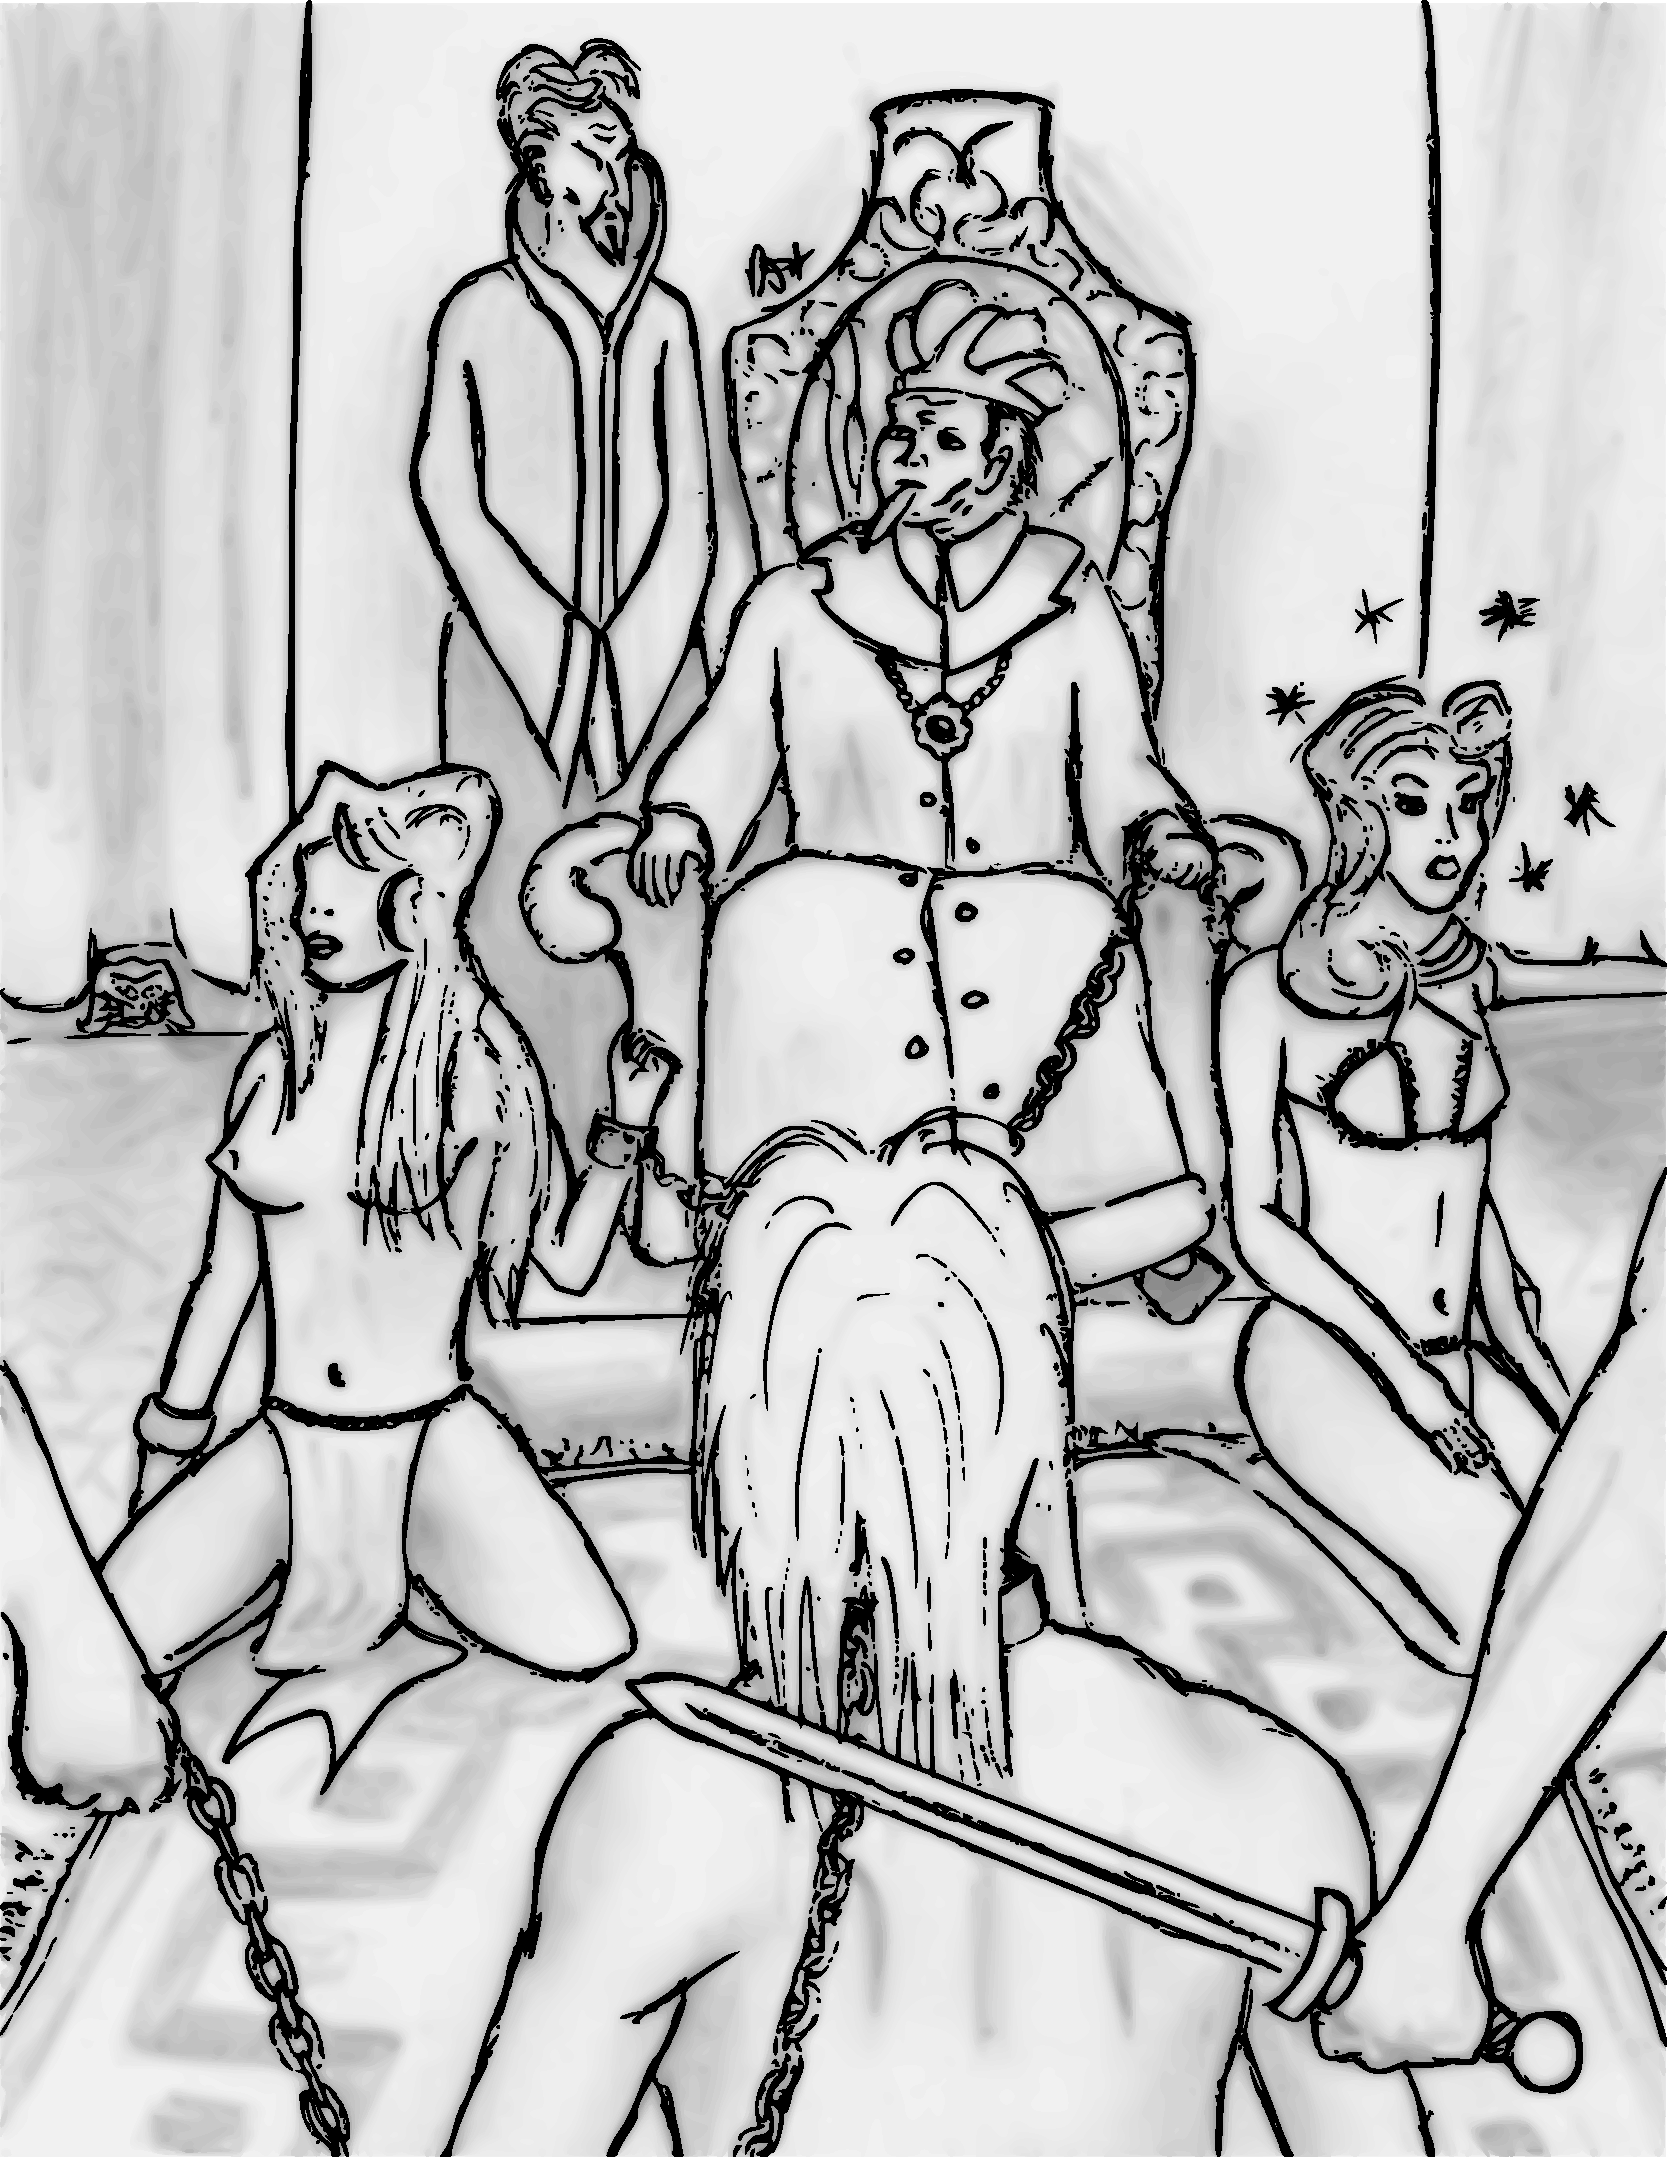
\includepdf[scale=1.007]{grignrchained.pdf}


